\chapter{Conversational Group Detection}\label{ch.fformation}

The literature presented in \cref{sec.rw.hi.unfocused} suggests that people, who perceive an agent as \glsatt{copresence}, show similar behaviours and have similar expectations towards it as in interactions with humans.
To be accepted in long term interactions, agents therefore need to understand these behaviours and the implied expectations.
They need to know when to interact and when to show \gls{civil inattention} (\cref{sec.rw.hi.focused-rw.perception}).
Without distinguishing participants of the agents \gls{conversational group} from \glspl{non-participant}, it can not treat them accordingly. 
The detection of \glspl{conversational group} in the presence of humans and \gls{artificial agent} is therefore an important basis for \gls{conversational role} recognition and behaviour recognition.
Therefore, I investigate \Cref{hyp.fformation}\rqnote{hyp.fformation}{\hypfformation} in this chapter.
To this end, I use the corpus of unconstrained, mixed human-agent interactions presented in \cref{sec.group.corpus}. 
Because of the discussed similarities between peoples behaviour towards humans and \glspl{artificial agent}, I investigate this research question by examining the following claim: 
\newcommand{\hypffmone}{Mixed \glspl{conversational group} of people and \glspl{artificial agent} can be detected using \glspl{ffm} as known from \gls{hhi}.}
\begin{hyp3}[Group from \gls{ffm}]
    \label{ffm.h1}
    \hypffmone
\end{hyp3}
It is often sufficient to know if the agent is in a group or not without identifying the participants of the group. 
Furthermore, the detection of \glspl{ffm} requires a good understanding of the distribution of persons in the scene which can be computationally expensive and not always feasible.
Therefore, I propose the following simplifications for comparison:
\newcommand{\hypffmgaze}{The detection of peoples ga\-ze di\-rec\-tion in the agents field of view can sufficiently inform about whether it is in a \gls{conversational group} or not.}
\begin{hyp3}[Group from Mutual Gaze]
    \label{ffm.gaze}
    \hypffmgaze
\end{hyp3}
\newcommand{\hypffmface}{The detection of faces in the agents field of view can sufficiently inform about whether it is in a \gls{conversational group} or not.}
\begin{hyp3}[Group from Faces]
    \label{ffm.face}
    \hypffmface
\end{hyp3}


In this chapter I evaluate the detection of \glspl{conversational group} for \glspl{virtual agent} in a \gls{smart environment}.
To this end, I first evaluate \cref{ffm.h1}---the portability of \gls{ffm} detection as presented by~\citewithauthor{Setti2015} from human groups to mixed human-agent groups---on automatically extracted data (see \cref{sec.fformation.fformation}).
Subsequently, I evaluate \cref{ffm.gaze,ffm.face} by testing if the agents' participation in a \gls{conversational group} can be deduced from gaze directions and detected face sizes (see \cref{sec.fformation.inout}).

\section{F-Formation Detection}\label{sec.fformation.fformation}

The participants of a \gls{conversational group} need to optimize their mutual access to the joint interaction space (\gls{ospace}).
This is achieved by overlapping their \glspl{transactional segment} (\cref{sec.rw.hi.focused}).
One approach for \gls{ffm}-detection in \gls{hhi}, is presented by~\citewithauthor{Setti2015}.
It uses 2D positions \([x,y]\) and orientations \(\theta\) of persons in an open space to estimate the centres of their \glspl{transactional segment} (\(TS\)).
This segment is assumed to be in front of the person with its centre at a fixed distance called \gls{stride} (\(S\)).
Based on the distance between the \(TS\) and the \gls{ospace} of a potential group and its visibility for a person, a cost function can be created.
This cost-function should be zero for a perfect overlap of \gls{transactional segment} and \gls{ospace} without obstacles, and grow when they move apart or the \gls{ospace} is occluded.
A good assignment of persons to \glspl{conversational group} can then be found by optimizing the overall costs for a scene. 
In \cref{fig:ffm.approach} an exemplary scene can be seen with visualizations of the relevant variables.
The used variables are explained in the next subsection.
\begin{figure}[htbp]
    \centering
    \def\svgwidth{1.0\textwidth}
    \input{generated/fformation-costs.pdf_tex}
    \caption[F-Formation detection scene.]{\label{fig:ffm.approach}
    A visualization of a scene in the \gls{ffm} detection.
    People (\(P_i\)) are defined as positions \([ x_i, y_i ]\) (green points) with an optional orientation \(\theta_i\).
    \(P_2\) is shown as a circle because there is no known orientation.
    Centres of \glspl{transactional segment} (\(TS_i = [x_{\mu_i},y_{\mu_i}]\), blue points) are at the distance \(S\) (\gls{stride}) in front of persons or---when orientation is unknown---at their position (\(TS_2=P_2\)).
    \(P_3\) and \(P_5\) form the \gls{conversational group} \(G_1\) (gray dashed circle) with the \gls{ospace} centre \(O(G_1)\) (red dot).
    \(P_4\) is not part of \(G_1\) because the \gls{ospace} is occluded by \(P_3\).
    The \glspl{transactional segment} of \(P_1\) and \(P_2\) are too far away from \(O(G_1)\) for them to be part of the group.
    The distances \(d^1_1\) and \(d^1_2\) represent the distance between the \gls{ospace} centre \(O(G_1)\) (superscript index) and the position of \(P_1\) or \(P_2\) (subscript index) respectively.
    The angle \(\theta^1_{1,2}\) is the angle between \(P_1\) and \(P_2\) (subscript index) regarding the \gls{ospace} centre \(O(G_1)\) (superscript index).
    }
\end{figure}

To investigate if this approach can be used to detect \glspl{conversational group} with an \gls{artificial agent}, I create the open-source group detection framework~\citesoft{ffm}.
It models observations of persons and the cost of assigning them to \glspl{conversational group} according to the cost function presented by~\citewithauthor{Setti2015} with an adaptation to cover observations with unknown orientation.

\subsection{Assignment Costs \& Detectors}\label{sec.fformation.formation.detectors}

The cost function is drawn from~\citewithauthor{Setti2015}.
The calculation is done with the following definitions in mind:
An observation is defined as a set of persons \(P = \{P_1,\dots,P_n\}\) with 2D positions and orientations---i.e. \(P_i = [x_i, y_i, \theta_i]\).
From a person's pose, the \gls{transactional segment} \(TS_i\) can be computed using the \gls{stride} (\(S\)), which encodes the expected distance between a persons position and \gls{transactional segment}.
If the orientation of a person is not known, the \(TS_i\) can not be computed.
Therefore, I extend the \(TS_i\) formula to return the original position of the person when the orientation is not known.
This equals to the mean \(TS_i\) over all possible orientations.
The calculation of \glspl{transactional segment} is visualized in \cref{fig:ffm.approach} and formalized as follows:
\[
    TS_i = [x_{\mu_i},y_{\mu_i}] = 
    \begin{cases}
        [x_i + S\text{cos}(\theta_i)], y_i + S \text{sin} \theta_i],& \text{if }\theta_i\text{ is known} \\
        [x_i, y_i],& \text{otherwise}
    \end{cases}
\]
This allows calculating \(TS = \{TS_1,\dots,TS_n\}\) from \(P = \{P_1,\dots,P_n\}\).

An assignment of persons to groups is defined as the set of groups \(G = \{G_1,\dots,G_m\}\) with each person assigned to exactly one group.
Groups with \(|G_k|=1\) are allowed and represent persons that do not participate in a \gls{conversational group}.
Consequently, the group of person \(P_i\) is unambiguous and can be defined as \(g(P_i)\).
The \gls{ospace}-centre \(O(G_k)\) of a group \(G_k\) is calculated from the \glspl{transactional segment} of its participants.
\[
    O(G_k) = [u_{G_k}, v_{G_k}] = \frac{\sum_{i \in G_k}{TS_i}}{|G_k|}
\]
The \gls{ospace}-centre that corresponds to the group of \(P_i\) is therefore: 
\[
    O(g(P_i)) = [u_{g(P_i)},v_{g(P_i)}]
 \]

\paragraph{Assignment Cost}

The overall cost of an assignment \(G\) (\cref{eq:ffm.cost}) is calculated as the sum of \gls{ospace}-distance costs (\cref{eq:ffm.cost1}), \gls{ospace}-visibility costs (\cref{eq:ffm.cost2}) and an additional \gls{mdl}-prior (\cref{eq:ffm.cost3}):
\begin{equation}\label{eq:ffm.cost}
    \underbrace{C(G)}_{\text{assignment cost}} = \underbrace{D(G)}_{\text{distance cost}} + \underbrace{V(G|P)}_{\text{visibility cost}} + \underbrace{P(G)}_{\text{\gls{mdl}-prior}}
\end{equation}
The different parts of the formula are explained in the following.
A detailed motivation and in-depth analysis of this cost function can be looked up from ~\citewithauthor{Setti2015}.

\paragraph{Distance Cost}

The \emph{distance cost} \(D(G)\) penalizes deviations of \gls{transactional segment} centres from the groups' \gls{ospace}.
It therefore is zero when the \glspl{transactional segment} of the participants and the \gls{ospace} perfectly overlap and rises when the distance between \gls{transactional segment} and \gls{ospace} centre grows.
A high distance cost, means that the \gls{ospace} is too far away from the person to be maintained effectively.
The distance cost is calculated as follows:
\begin{equation}\label{eq:ffm.cost1}
     D(G) = \sum_{i \in P}{(u_{g(P_i)}-x_{\mu_i})^2+(v_{g(P_i)}-y_{\mu_i})^2}
\end{equation}

\paragraph{Visibility Cost}
The \emph{visibility cost} ensures that the \gls{ospace} \(O(g(P_i))\) of a person \(P_i\)'s \gls{conversational group} is not occluded by any other person \(P_{j \neq i}\).
Because the visibility can be occluded by any other person in the scene, the overall visibility cost for an assignment is the sum over the visibility constraint for all two-person permutations from \(P\):
\begin{equation}\label{eq:ffm.cost2}
    V(G) = \sum_{i,j \in P, i \neq j}{\underbrace{R_{i,j}(g(P_i))}_{\text{visibility constraint}}}
\end{equation}
The \emph{visibility constraint} can be calculated for a combination of two persons \(P_i\), \(P_j\), and a group centre \(O(G_k)\).
To not disrupt \(P_i\)'s visibility to the \gls{ospace}-centre, \(P_j\) must either stand farther away than \(P_i\) or on a different side of it.
The first can be ensured by comparing their distances to \(O(G_k)\), and the second by considering the angle between them regarding the same \(O(G_k)\).
To this end, \(d^k_i\) is defined as the distance between the position of \(P_i\) and \(O(G_k)\), and \(\theta^k_{i,j}\) is the angle between \(P_i\) and \(P_j\) regarding \(O(G_k)\).
An exemplary visualization of these measurements can be seen in \cref{fig:ffm.approach}.
The relevance of occlusions can be adjusted with a constant factor \(K\) for angles between \(0\) and a cut-off \(\hat{\theta}\).
As applied in the evaluations by~\citewithauthor{Setti2015}, these are chosen as \(\hat{\theta} = 0.75\) and \(K = 100\) for the evaluations in this chapter.
On this basis, the visibility constraint for any combination of \(P_i\), \(P_j\), and \(G_k\) calculates as follows:
\[
    R_{i,j}(G_k) = 
    \begin{cases}
        0,& \text{if }\theta^k_{i,j} > \hat{\theta}\text{ or }d^k_i < d^k_j \\
        \text{exp}(K\text{cos}(\theta^k_{i,j}))\frac{d^k_i-d^k_j}{d^k_j},& \text{otherwise}
    \end{cases}
\]

\paragraph{MDL-Prior}

Finally, \cref{eq:ffm.cost1,eq:ffm.cost2} both result in zero assignment costs for \(|G_k|=1\).
Therefore, an additional term is required to penalize small groups.
This is achieved by adding an \emph{\gls{mdl}-prior} over the amount of groups, which can be adapted with the parameter \(M\):
\begin{equation}\label{eq:ffm.cost3}
     P(G) = M|G|
\end{equation}

An assignment of persons in a scene to \glspl{conversational group} can be created by optimizing the cost function in \cref{eq:ffm.cost}.
To this end, I implement three different detectors:
(1) Detector \emph{Gco} from~\citesoft{ffm-gco}: uses ~\citesoftware{gco} to implement the approach from~\citewithauthor{Setti2015}.
For comparison, the original implementation can be found in~\citesoftware{gcff}.
The detectors (2) \emph{Shrink} and (3) \emph{Grow} from~\citesoft{ffm} use \emph{k-means} to find the best assignment for a fixed number of groups.
To find the best number of groups, \emph{shrink} increases it starting from one---thereby shrinking the group size---as long as the cost decreases.
\emph{Grow} starts with one group for each person and reduces the amount of groups as long as the cost decreases.
Finally, two dummy detectors are available: \emph{None} always returns a group for each person and \emph{One} always assigns all persons to a single group \cite{ffm}.
By applying these detectors to the created corpus, I can investigate \cref{ffm.h1}\rqnote{ffm.h1}{\hypffmone}.

\subsection{Evaluation}

To evaluate \cref{ffm.h1}, I use the ground truth annotations of group assignments and person positions from both the annotations and the automatic detections.
An evaluation of the \gls{ffm} detection for \gls{hhi} is already done by~\citewithauthor{Setti2015}.
Because the evaluation in this section is concerned with the quality of detected \glspl{conversational group} of \glspl{artificial agent}, a quality metric is required that can be applied to a single agent in the scene separately.
To this end, I use the definition of a \gls{tolerant match} by~\citewithauthor{Setti2015}:
\begin{definition}[Tolerant Match]
    \label{def.tm}
     With a threshold \(T \in [0,1]\) (\gls{tolerance threshold}), a predicted group \(G_k\) is a \emph{tolerant match} if at least \(T|G_k|\) participants of the group are correctly assigned and less than \(1-T|G_k|\) participants are falsely assigned to it~\cite[]{Setti2015}.
\end{definition}
The choice of \(T\) determines how exact the detected group must match the ground truth to be correct.
\begin{corollary}
    \label{cor.tm.1}
    Tolerant matches for \(T < \frac{1}{2}\) classify groups with more than 50\% wrong or missing persons as correct.
\end{corollary}
With this definition, a \gls{confusion matrix} can be calculated.
In contrast to~\citewithauthor{Setti2015}, the \glspl{confusion matrix} in this section are calculated for each agent separately.
The matrix is calculated as sums of observations where:
\begin{description}
    \item[\acrshort{tp}:] the agent is correctly assigned to a group and the group matches the annotation according to the \gls{tolerant match}.
    \item[\acrshort{fp}:] the agent is falsely assigned to any group.
    \item[\acrshort{tn}:] the agent is correctly classified as not in a group.
    \item[\acrshort{fn}:] the agent is falsely classified as not in a group or assigned to the wrong group according to the \gls{tolerant match}\footnote{Counting an assignment to the wrong group when the agent is in a group as \acrlong{fn} may seem counter-intuitive.
    However, \acrlong{fp} implies that the agent is not in a group.
    This case can be interpreted as: falsely not assigning to the correct group (\acrlong{fn}).
    }.
\end{description}
By definition, the agent is always a participant of it's own group: \(P_i \in g(P_i)\).
Therefore, it is always correctly assigned and the match is always greater than 0.
\begin{corollary}
    \label{cor.tm.2}
    With \(T=\frac{1}{|P|+1}\) the \gls{confusion matrix} measures the detection of the agent being in a group or not, regardless the other participants of the group.
\end{corollary}
On the basis of these measures, four detector configurations are chosen from a grid search on \gls{mdl}, \gls{stride}, and algorithm.
For the range of \(T \in [0.5,1]\) (\cref{cor.tm.1}), the usual quality measurements are calculated over the whole corpus and visualized for each agent on annotated and detected person percepts.
The detected percepts are the fusion results from the \gls{apartment}'s person tracking and \citewithauthor{openposegit} based detections.
The resulting plot can be seen in \cref{fig:ffm-ffm} and is analysed in the following.
\begin{figure}[tbhp]
    \centering
    %\fbox{\begin{minipage}{\textwidth}
    %\fbox{
    \small
    % Created by tikzDevice version 0.12
% !TEX encoding = UTF-8 Unicode
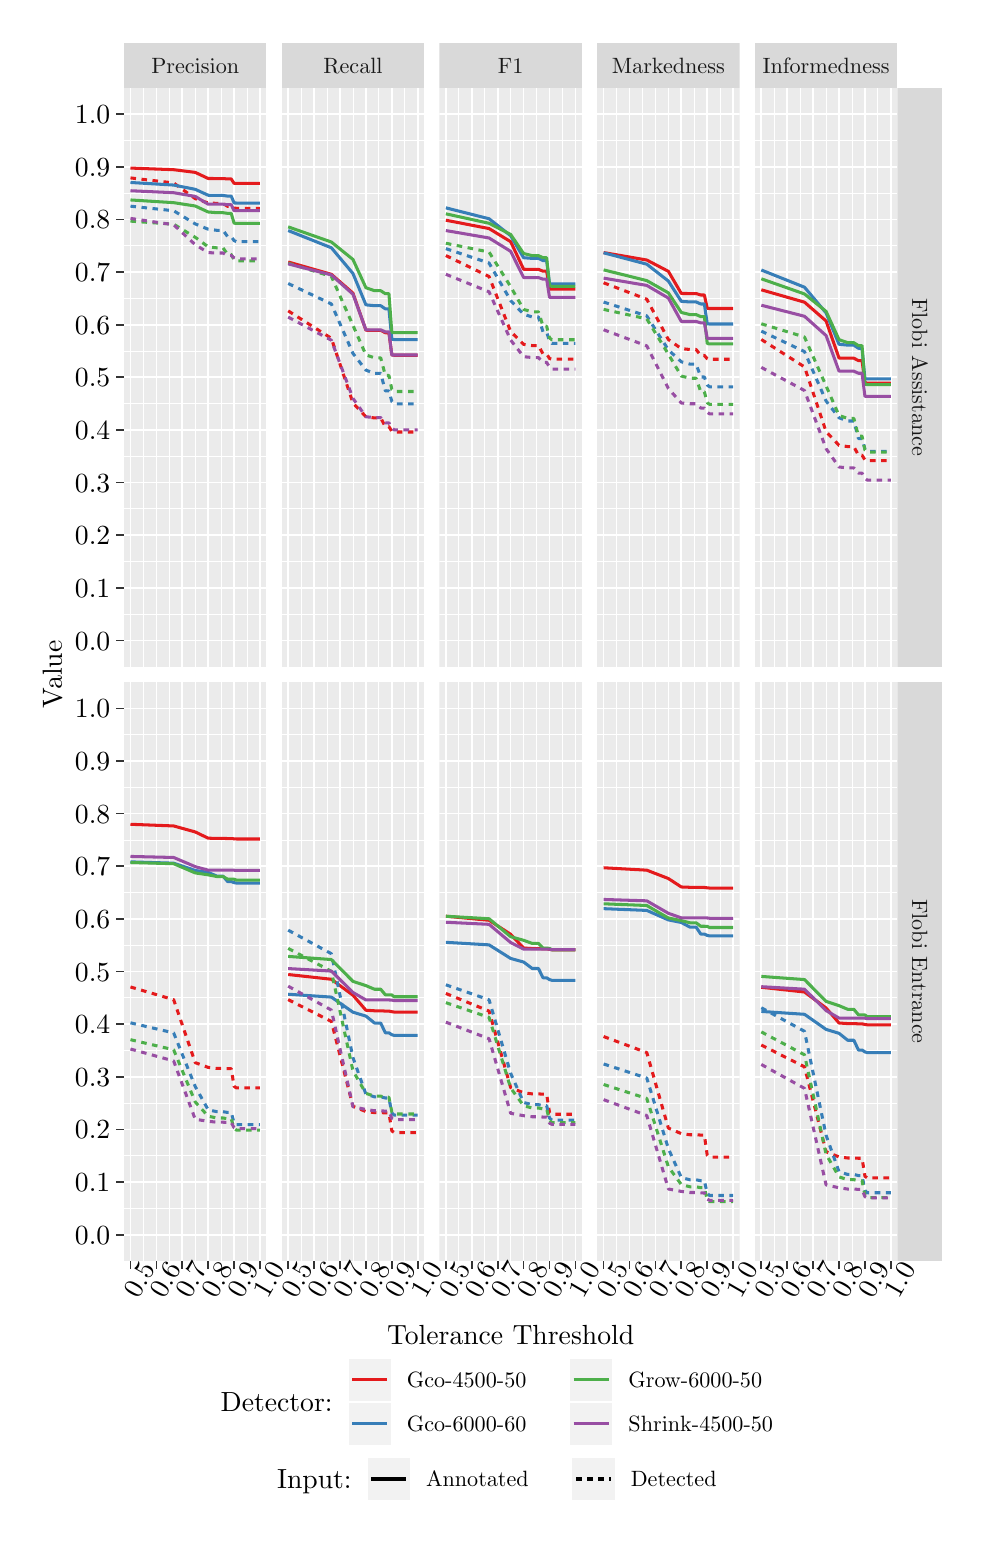
\begin{tikzpicture}[x=1pt,y=1pt]
\definecolor{fillColor}{RGB}{255,255,255}
\path[use as bounding box,fill=fillColor,fill opacity=0.00] (0,0) rectangle (336.00,539.88);
\begin{scope}
\path[clip] (  0.00,  0.00) rectangle (336.00,539.88);
\definecolor{drawColor}{RGB}{255,255,255}
\definecolor{fillColor}{RGB}{255,255,255}

\path[draw=drawColor,line width= 0.6pt,line join=round,line cap=round,fill=fillColor] (  0.00,  0.00) rectangle (336.00,539.88);
\end{scope}
\begin{scope}
\path[clip] ( 34.81,308.92) rectangle ( 86.29,518.13);
\definecolor{fillColor}{gray}{0.92}

\path[fill=fillColor] ( 34.81,308.92) rectangle ( 86.29,518.13);
\definecolor{drawColor}{RGB}{255,255,255}

\path[draw=drawColor,line width= 0.3pt,line join=round] ( 34.81,327.94) --
	( 86.29,327.94);

\path[draw=drawColor,line width= 0.3pt,line join=round] ( 34.81,346.96) --
	( 86.29,346.96);

\path[draw=drawColor,line width= 0.3pt,line join=round] ( 34.81,365.98) --
	( 86.29,365.98);

\path[draw=drawColor,line width= 0.3pt,line join=round] ( 34.81,385.00) --
	( 86.29,385.00);

\path[draw=drawColor,line width= 0.3pt,line join=round] ( 34.81,404.02) --
	( 86.29,404.02);

\path[draw=drawColor,line width= 0.3pt,line join=round] ( 34.81,423.03) --
	( 86.29,423.03);

\path[draw=drawColor,line width= 0.3pt,line join=round] ( 34.81,442.05) --
	( 86.29,442.05);

\path[draw=drawColor,line width= 0.3pt,line join=round] ( 34.81,461.07) --
	( 86.29,461.07);

\path[draw=drawColor,line width= 0.3pt,line join=round] ( 34.81,480.09) --
	( 86.29,480.09);

\path[draw=drawColor,line width= 0.3pt,line join=round] ( 34.81,499.11) --
	( 86.29,499.11);

\path[draw=drawColor,line width= 0.3pt,line join=round] ( 41.83,308.92) --
	( 41.83,518.13);

\path[draw=drawColor,line width= 0.3pt,line join=round] ( 46.51,308.92) --
	( 46.51,518.13);

\path[draw=drawColor,line width= 0.3pt,line join=round] ( 51.19,308.92) --
	( 51.19,518.13);

\path[draw=drawColor,line width= 0.3pt,line join=round] ( 55.87,308.92) --
	( 55.87,518.13);

\path[draw=drawColor,line width= 0.3pt,line join=round] ( 60.55,308.92) --
	( 60.55,518.13);

\path[draw=drawColor,line width= 0.3pt,line join=round] ( 69.91,308.92) --
	( 69.91,518.13);

\path[draw=drawColor,line width= 0.3pt,line join=round] ( 79.27,308.92) --
	( 79.27,518.13);

\path[draw=drawColor,line width= 0.6pt,line join=round] ( 34.81,318.43) --
	( 86.29,318.43);

\path[draw=drawColor,line width= 0.6pt,line join=round] ( 34.81,337.45) --
	( 86.29,337.45);

\path[draw=drawColor,line width= 0.6pt,line join=round] ( 34.81,356.47) --
	( 86.29,356.47);

\path[draw=drawColor,line width= 0.6pt,line join=round] ( 34.81,375.49) --
	( 86.29,375.49);

\path[draw=drawColor,line width= 0.6pt,line join=round] ( 34.81,394.51) --
	( 86.29,394.51);

\path[draw=drawColor,line width= 0.6pt,line join=round] ( 34.81,413.53) --
	( 86.29,413.53);

\path[draw=drawColor,line width= 0.6pt,line join=round] ( 34.81,432.54) --
	( 86.29,432.54);

\path[draw=drawColor,line width= 0.6pt,line join=round] ( 34.81,451.56) --
	( 86.29,451.56);

\path[draw=drawColor,line width= 0.6pt,line join=round] ( 34.81,470.58) --
	( 86.29,470.58);

\path[draw=drawColor,line width= 0.6pt,line join=round] ( 34.81,489.60) --
	( 86.29,489.60);

\path[draw=drawColor,line width= 0.6pt,line join=round] ( 34.81,508.62) --
	( 86.29,508.62);

\path[draw=drawColor,line width= 0.6pt,line join=round] ( 37.15,308.92) --
	( 37.15,518.13);

\path[draw=drawColor,line width= 0.6pt,line join=round] ( 46.51,308.92) --
	( 46.51,518.13);

\path[draw=drawColor,line width= 0.6pt,line join=round] ( 55.87,308.92) --
	( 55.87,518.13);

\path[draw=drawColor,line width= 0.6pt,line join=round] ( 65.23,308.92) --
	( 65.23,518.13);

\path[draw=drawColor,line width= 0.6pt,line join=round] ( 74.59,308.92) --
	( 74.59,518.13);

\path[draw=drawColor,line width= 0.6pt,line join=round] ( 83.95,308.92) --
	( 83.95,518.13);
\definecolor{drawColor}{RGB}{228,26,28}

\path[draw=drawColor,line width= 1.1pt,line join=round] ( 37.15,489.14) --
	( 52.75,488.55) --
	( 60.55,487.58) --
	( 65.23,485.37) --
	( 68.35,485.36) --
	( 70.58,485.36) --
	( 72.25,485.21) --
	( 73.55,485.21) --
	( 74.59,483.63) --
	( 75.44,483.60) --
	( 76.15,483.60) --
	( 83.94,483.60);

\path[draw=drawColor,line width= 1.1pt,dash pattern=on 2pt off 2pt ,line join=round] ( 37.15,485.58) --
	( 52.75,483.77) --
	( 60.55,478.08) --
	( 65.23,476.53) --
	( 68.35,476.38) --
	( 70.58,476.38) --
	( 72.25,475.30) --
	( 73.55,475.30) --
	( 74.59,474.69) --
	( 75.44,474.60) --
	( 76.15,474.60) --
	( 83.94,474.60);
\definecolor{drawColor}{RGB}{55,126,184}

\path[draw=drawColor,line width= 1.1pt,line join=round] ( 37.15,483.94) --
	( 52.75,483.00) --
	( 60.55,481.46) --
	( 65.23,479.32) --
	( 68.35,479.25) --
	( 70.58,479.25) --
	( 72.25,479.01) --
	( 73.55,479.01) --
	( 74.59,476.53) --
	( 75.44,476.51) --
	( 76.15,476.51) --
	( 83.94,476.51);

\path[draw=drawColor,line width= 1.1pt,dash pattern=on 2pt off 2pt ,line join=round] ( 37.15,475.37) --
	( 52.75,473.72) --
	( 60.55,468.97) --
	( 65.23,467.04) --
	( 68.35,466.65) --
	( 70.58,466.65) --
	( 72.25,464.39) --
	( 73.55,464.39) --
	( 74.59,462.92) --
	( 75.44,462.56) --
	( 76.15,462.56) --
	( 83.94,462.56);
\definecolor{drawColor}{RGB}{77,175,74}

\path[draw=drawColor,line width= 1.1pt,line join=round] ( 37.15,477.62) --
	( 52.75,476.64) --
	( 60.55,475.43) --
	( 65.23,473.27) --
	( 68.35,473.02) --
	( 70.58,473.02) --
	( 72.25,472.77) --
	( 73.55,472.77) --
	( 74.59,469.22) --
	( 75.44,469.17) --
	( 76.15,469.17) --
	( 83.94,469.17);

\path[draw=drawColor,line width= 1.1pt,dash pattern=on 2pt off 2pt ,line join=round] ( 37.15,469.97) --
	( 52.75,468.86) --
	( 60.55,464.13) --
	( 65.23,460.68) --
	( 68.35,460.32) --
	( 70.58,460.32) --
	( 72.25,457.95) --
	( 73.55,457.95) --
	( 74.59,455.93) --
	( 75.44,455.60) --
	( 76.15,455.60) --
	( 83.94,455.60);
\definecolor{drawColor}{RGB}{152,78,163}

\path[draw=drawColor,line width= 1.1pt,line join=round] ( 37.15,480.95) --
	( 52.75,480.24) --
	( 60.55,478.90) --
	( 65.23,476.08) --
	( 68.35,476.08) --
	( 70.58,476.08) --
	( 72.25,475.90) --
	( 73.55,475.90) --
	( 74.59,473.74) --
	( 75.44,473.74) --
	( 76.15,473.74) --
	( 83.94,473.74);

\path[draw=drawColor,line width= 1.1pt,dash pattern=on 2pt off 2pt ,line join=round] ( 37.15,470.95) --
	( 52.75,468.66) --
	( 60.55,461.45) --
	( 65.23,458.59) --
	( 68.35,458.45) --
	( 70.58,458.45) --
	( 72.25,457.57) --
	( 73.55,457.57) --
	( 74.59,456.70) --
	( 75.44,456.33) --
	( 76.15,456.33) --
	( 83.94,456.33);
\end{scope}
\begin{scope}
\path[clip] ( 34.81, 94.21) rectangle ( 86.29,303.42);
\definecolor{fillColor}{gray}{0.92}

\path[fill=fillColor] ( 34.81, 94.21) rectangle ( 86.29,303.42);
\definecolor{drawColor}{RGB}{255,255,255}

\path[draw=drawColor,line width= 0.3pt,line join=round] ( 34.81,113.23) --
	( 86.29,113.23);

\path[draw=drawColor,line width= 0.3pt,line join=round] ( 34.81,132.25) --
	( 86.29,132.25);

\path[draw=drawColor,line width= 0.3pt,line join=round] ( 34.81,151.27) --
	( 86.29,151.27);

\path[draw=drawColor,line width= 0.3pt,line join=round] ( 34.81,170.29) --
	( 86.29,170.29);

\path[draw=drawColor,line width= 0.3pt,line join=round] ( 34.81,189.30) --
	( 86.29,189.30);

\path[draw=drawColor,line width= 0.3pt,line join=round] ( 34.81,208.32) --
	( 86.29,208.32);

\path[draw=drawColor,line width= 0.3pt,line join=round] ( 34.81,227.34) --
	( 86.29,227.34);

\path[draw=drawColor,line width= 0.3pt,line join=round] ( 34.81,246.36) --
	( 86.29,246.36);

\path[draw=drawColor,line width= 0.3pt,line join=round] ( 34.81,265.38) --
	( 86.29,265.38);

\path[draw=drawColor,line width= 0.3pt,line join=round] ( 34.81,284.40) --
	( 86.29,284.40);

\path[draw=drawColor,line width= 0.3pt,line join=round] ( 41.83, 94.21) --
	( 41.83,303.42);

\path[draw=drawColor,line width= 0.3pt,line join=round] ( 46.51, 94.21) --
	( 46.51,303.42);

\path[draw=drawColor,line width= 0.3pt,line join=round] ( 51.19, 94.21) --
	( 51.19,303.42);

\path[draw=drawColor,line width= 0.3pt,line join=round] ( 55.87, 94.21) --
	( 55.87,303.42);

\path[draw=drawColor,line width= 0.3pt,line join=round] ( 60.55, 94.21) --
	( 60.55,303.42);

\path[draw=drawColor,line width= 0.3pt,line join=round] ( 69.91, 94.21) --
	( 69.91,303.42);

\path[draw=drawColor,line width= 0.3pt,line join=round] ( 79.27, 94.21) --
	( 79.27,303.42);

\path[draw=drawColor,line width= 0.6pt,line join=round] ( 34.81,103.72) --
	( 86.29,103.72);

\path[draw=drawColor,line width= 0.6pt,line join=round] ( 34.81,122.74) --
	( 86.29,122.74);

\path[draw=drawColor,line width= 0.6pt,line join=round] ( 34.81,141.76) --
	( 86.29,141.76);

\path[draw=drawColor,line width= 0.6pt,line join=round] ( 34.81,160.78) --
	( 86.29,160.78);

\path[draw=drawColor,line width= 0.6pt,line join=round] ( 34.81,179.79) --
	( 86.29,179.79);

\path[draw=drawColor,line width= 0.6pt,line join=round] ( 34.81,198.81) --
	( 86.29,198.81);

\path[draw=drawColor,line width= 0.6pt,line join=round] ( 34.81,217.83) --
	( 86.29,217.83);

\path[draw=drawColor,line width= 0.6pt,line join=round] ( 34.81,236.85) --
	( 86.29,236.85);

\path[draw=drawColor,line width= 0.6pt,line join=round] ( 34.81,255.87) --
	( 86.29,255.87);

\path[draw=drawColor,line width= 0.6pt,line join=round] ( 34.81,274.89) --
	( 86.29,274.89);

\path[draw=drawColor,line width= 0.6pt,line join=round] ( 34.81,293.91) --
	( 86.29,293.91);

\path[draw=drawColor,line width= 0.6pt,line join=round] ( 37.15, 94.21) --
	( 37.15,303.42);

\path[draw=drawColor,line width= 0.6pt,line join=round] ( 46.51, 94.21) --
	( 46.51,303.42);

\path[draw=drawColor,line width= 0.6pt,line join=round] ( 55.87, 94.21) --
	( 55.87,303.42);

\path[draw=drawColor,line width= 0.6pt,line join=round] ( 65.23, 94.21) --
	( 65.23,303.42);

\path[draw=drawColor,line width= 0.6pt,line join=round] ( 74.59, 94.21) --
	( 74.59,303.42);

\path[draw=drawColor,line width= 0.6pt,line join=round] ( 83.95, 94.21) --
	( 83.95,303.42);
\definecolor{drawColor}{RGB}{228,26,28}

\path[draw=drawColor,line width= 1.1pt,line join=round] ( 37.15,252.02) --
	( 52.75,251.42) --
	( 60.55,249.25) --
	( 65.23,247.00) --
	( 68.35,246.91) --
	( 70.58,246.91) --
	( 72.25,246.87) --
	( 73.55,246.87) --
	( 74.59,246.77) --
	( 75.44,246.71) --
	( 76.15,246.71) --
	( 83.94,246.71);

\path[draw=drawColor,line width= 1.1pt,dash pattern=on 2pt off 2pt ,line join=round] ( 37.15,193.24) --
	( 52.75,188.64) --
	( 60.55,165.89) --
	( 65.23,164.17) --
	( 68.35,163.81) --
	( 70.58,163.81) --
	( 72.25,163.72) --
	( 73.55,163.72) --
	( 74.59,157.34) --
	( 75.44,156.74) --
	( 76.15,156.74) --
	( 83.94,156.74);
\definecolor{drawColor}{RGB}{55,126,184}

\path[draw=drawColor,line width= 1.1pt,line join=round] ( 37.15,238.44) --
	( 52.75,237.97) --
	( 60.55,235.34) --
	( 65.23,234.62) --
	( 68.35,233.30) --
	( 70.58,233.30) --
	( 72.25,231.32) --
	( 73.55,231.32) --
	( 74.59,230.93) --
	( 75.44,230.78) --
	( 76.15,230.78) --
	( 83.94,230.78);

\path[draw=drawColor,line width= 1.1pt,dash pattern=on 2pt off 2pt ,line join=round] ( 37.15,180.28) --
	( 52.75,176.64) --
	( 60.55,157.26) --
	( 65.23,148.83) --
	( 68.35,148.17) --
	( 70.58,148.17) --
	( 72.25,147.89) --
	( 73.55,147.89) --
	( 74.59,144.10) --
	( 75.44,143.51) --
	( 76.15,143.51) --
	( 83.94,143.51);
\definecolor{drawColor}{RGB}{77,175,74}

\path[draw=drawColor,line width= 1.1pt,line join=round] ( 37.15,238.22) --
	( 52.75,237.77) --
	( 60.55,234.45) --
	( 65.23,233.75) --
	( 68.35,233.14) --
	( 70.58,233.14) --
	( 72.25,232.20) --
	( 73.55,232.20) --
	( 74.59,232.17) --
	( 75.44,231.86) --
	( 76.15,231.86) --
	( 83.94,231.86);

\path[draw=drawColor,line width= 1.1pt,dash pattern=on 2pt off 2pt ,line join=round] ( 37.15,174.19) --
	( 52.75,170.54) --
	( 60.55,151.68) --
	( 65.23,146.54) --
	( 68.35,145.89) --
	( 70.58,145.89) --
	( 72.25,145.62) --
	( 73.55,145.62) --
	( 74.59,142.10) --
	( 75.44,141.53) --
	( 76.15,141.53) --
	( 83.94,141.53);
\definecolor{drawColor}{RGB}{152,78,163}

\path[draw=drawColor,line width= 1.1pt,line join=round] ( 37.15,240.40) --
	( 52.75,240.03) --
	( 60.55,236.71) --
	( 65.23,235.44) --
	( 68.35,235.44) --
	( 70.58,235.44) --
	( 72.25,235.44) --
	( 73.55,235.44) --
	( 74.59,235.42) --
	( 75.44,235.33) --
	( 76.15,235.33) --
	( 83.94,235.33);

\path[draw=drawColor,line width= 1.1pt,dash pattern=on 2pt off 2pt ,line join=round] ( 37.15,170.82) --
	( 52.75,166.50) --
	( 60.55,145.42) --
	( 65.23,144.70) --
	( 68.35,144.37) --
	( 70.58,144.37) --
	( 72.25,144.28) --
	( 73.55,144.28) --
	( 74.59,142.38) --
	( 75.44,142.04) --
	( 76.15,142.04) --
	( 83.94,142.04);
\end{scope}
\begin{scope}
\path[clip] ( 91.79,308.92) rectangle (143.28,518.13);
\definecolor{fillColor}{gray}{0.92}

\path[fill=fillColor] ( 91.79,308.92) rectangle (143.28,518.13);
\definecolor{drawColor}{RGB}{255,255,255}

\path[draw=drawColor,line width= 0.3pt,line join=round] ( 91.79,327.94) --
	(143.28,327.94);

\path[draw=drawColor,line width= 0.3pt,line join=round] ( 91.79,346.96) --
	(143.28,346.96);

\path[draw=drawColor,line width= 0.3pt,line join=round] ( 91.79,365.98) --
	(143.28,365.98);

\path[draw=drawColor,line width= 0.3pt,line join=round] ( 91.79,385.00) --
	(143.28,385.00);

\path[draw=drawColor,line width= 0.3pt,line join=round] ( 91.79,404.02) --
	(143.28,404.02);

\path[draw=drawColor,line width= 0.3pt,line join=round] ( 91.79,423.03) --
	(143.28,423.03);

\path[draw=drawColor,line width= 0.3pt,line join=round] ( 91.79,442.05) --
	(143.28,442.05);

\path[draw=drawColor,line width= 0.3pt,line join=round] ( 91.79,461.07) --
	(143.28,461.07);

\path[draw=drawColor,line width= 0.3pt,line join=round] ( 91.79,480.09) --
	(143.28,480.09);

\path[draw=drawColor,line width= 0.3pt,line join=round] ( 91.79,499.11) --
	(143.28,499.11);

\path[draw=drawColor,line width= 0.3pt,line join=round] ( 98.82,308.92) --
	( 98.82,518.13);

\path[draw=drawColor,line width= 0.3pt,line join=round] (103.50,308.92) --
	(103.50,518.13);

\path[draw=drawColor,line width= 0.3pt,line join=round] (108.18,308.92) --
	(108.18,518.13);

\path[draw=drawColor,line width= 0.3pt,line join=round] (112.86,308.92) --
	(112.86,518.13);

\path[draw=drawColor,line width= 0.3pt,line join=round] (117.54,308.92) --
	(117.54,518.13);

\path[draw=drawColor,line width= 0.3pt,line join=round] (126.90,308.92) --
	(126.90,518.13);

\path[draw=drawColor,line width= 0.3pt,line join=round] (136.26,308.92) --
	(136.26,518.13);

\path[draw=drawColor,line width= 0.6pt,line join=round] ( 91.79,318.43) --
	(143.28,318.43);

\path[draw=drawColor,line width= 0.6pt,line join=round] ( 91.79,337.45) --
	(143.28,337.45);

\path[draw=drawColor,line width= 0.6pt,line join=round] ( 91.79,356.47) --
	(143.28,356.47);

\path[draw=drawColor,line width= 0.6pt,line join=round] ( 91.79,375.49) --
	(143.28,375.49);

\path[draw=drawColor,line width= 0.6pt,line join=round] ( 91.79,394.51) --
	(143.28,394.51);

\path[draw=drawColor,line width= 0.6pt,line join=round] ( 91.79,413.53) --
	(143.28,413.53);

\path[draw=drawColor,line width= 0.6pt,line join=round] ( 91.79,432.54) --
	(143.28,432.54);

\path[draw=drawColor,line width= 0.6pt,line join=round] ( 91.79,451.56) --
	(143.28,451.56);

\path[draw=drawColor,line width= 0.6pt,line join=round] ( 91.79,470.58) --
	(143.28,470.58);

\path[draw=drawColor,line width= 0.6pt,line join=round] ( 91.79,489.60) --
	(143.28,489.60);

\path[draw=drawColor,line width= 0.6pt,line join=round] ( 91.79,508.62) --
	(143.28,508.62);

\path[draw=drawColor,line width= 0.6pt,line join=round] ( 94.13,308.92) --
	( 94.13,518.13);

\path[draw=drawColor,line width= 0.6pt,line join=round] (103.50,308.92) --
	(103.50,518.13);

\path[draw=drawColor,line width= 0.6pt,line join=round] (112.86,308.92) --
	(112.86,518.13);

\path[draw=drawColor,line width= 0.6pt,line join=round] (122.22,308.92) --
	(122.22,518.13);

\path[draw=drawColor,line width= 0.6pt,line join=round] (131.58,308.92) --
	(131.58,518.13);

\path[draw=drawColor,line width= 0.6pt,line join=round] (140.94,308.92) --
	(140.94,518.13);
\definecolor{drawColor}{RGB}{228,26,28}

\path[draw=drawColor,line width= 1.1pt,line join=round] ( 94.13,455.21) --
	(109.74,450.75) --
	(117.54,443.96) --
	(122.22,430.55) --
	(125.34,430.50) --
	(127.57,430.50) --
	(129.24,429.64) --
	(130.54,429.64) --
	(131.58,421.65) --
	(132.43,421.50) --
	(133.14,421.50) --
	(140.93,421.50);

\path[draw=drawColor,line width= 1.1pt,dash pattern=on 2pt off 2pt ,line join=round] ( 94.13,437.54) --
	(109.74,427.62) --
	(117.54,404.24) --
	(122.22,399.30) --
	(125.34,398.84) --
	(127.57,398.84) --
	(129.24,395.70) --
	(130.54,395.70) --
	(131.58,394.03) --
	(132.43,393.77) --
	(133.14,393.77) --
	(140.93,393.77);
\definecolor{drawColor}{RGB}{55,126,184}

\path[draw=drawColor,line width= 1.1pt,line join=round] ( 94.13,466.56) --
	(109.74,460.34) --
	(117.54,451.04) --
	(122.22,439.72) --
	(125.34,439.41) --
	(127.57,439.41) --
	(129.24,438.26) --
	(130.54,438.26) --
	(131.58,427.28) --
	(132.43,427.18) --
	(133.14,427.18) --
	(140.93,427.18);

\path[draw=drawColor,line width= 1.1pt,dash pattern=on 2pt off 2pt ,line join=round] ( 94.13,447.43) --
	(109.74,440.04) --
	(117.54,422.18) --
	(122.22,416.12) --
	(125.34,414.95) --
	(127.57,414.95) --
	(129.24,408.62) --
	(130.54,408.62) --
	(131.58,404.82) --
	(132.43,403.94) --
	(133.14,403.94) --
	(140.93,403.94);
\definecolor{drawColor}{RGB}{77,175,74}

\path[draw=drawColor,line width= 1.1pt,line join=round] ( 94.13,467.90) --
	(109.74,462.42) --
	(117.54,456.12) --
	(122.22,445.91) --
	(125.34,444.82) --
	(127.57,444.82) --
	(129.24,443.74) --
	(130.54,443.74) --
	(131.58,429.84) --
	(132.43,429.65) --
	(133.14,429.65) --
	(140.93,429.65);

\path[draw=drawColor,line width= 1.1pt,dash pattern=on 2pt off 2pt ,line join=round] ( 94.13,454.77) --
	(109.74,449.99) --
	(117.54,432.33) --
	(122.22,421.63) --
	(125.34,420.58) --
	(127.57,420.58) --
	(129.24,414.19) --
	(130.54,414.19) --
	(131.58,409.18) --
	(132.43,408.41) --
	(133.14,408.41) --
	(140.93,408.41);
\definecolor{drawColor}{RGB}{152,78,163}

\path[draw=drawColor,line width= 1.1pt,line join=round] ( 94.13,454.52) --
	(109.74,450.53) --
	(117.54,443.56) --
	(122.22,430.69) --
	(125.34,430.69) --
	(127.57,430.69) --
	(129.24,429.94) --
	(130.54,429.94) --
	(131.58,421.59) --
	(132.43,421.59) --
	(133.14,421.59) --
	(140.93,421.59);

\path[draw=drawColor,line width= 1.1pt,dash pattern=on 2pt off 2pt ,line join=round] ( 94.13,435.29) --
	(109.74,426.93) --
	(117.54,405.93) --
	(122.22,399.28) --
	(125.34,398.96) --
	(127.57,398.96) --
	(129.24,397.08) --
	(130.54,397.08) --
	(131.58,395.28) --
	(132.43,394.54) --
	(133.14,394.54) --
	(140.93,394.54);
\end{scope}
\begin{scope}
\path[clip] ( 91.79, 94.21) rectangle (143.28,303.42);
\definecolor{fillColor}{gray}{0.92}

\path[fill=fillColor] ( 91.79, 94.21) rectangle (143.28,303.42);
\definecolor{drawColor}{RGB}{255,255,255}

\path[draw=drawColor,line width= 0.3pt,line join=round] ( 91.79,113.23) --
	(143.28,113.23);

\path[draw=drawColor,line width= 0.3pt,line join=round] ( 91.79,132.25) --
	(143.28,132.25);

\path[draw=drawColor,line width= 0.3pt,line join=round] ( 91.79,151.27) --
	(143.28,151.27);

\path[draw=drawColor,line width= 0.3pt,line join=round] ( 91.79,170.29) --
	(143.28,170.29);

\path[draw=drawColor,line width= 0.3pt,line join=round] ( 91.79,189.30) --
	(143.28,189.30);

\path[draw=drawColor,line width= 0.3pt,line join=round] ( 91.79,208.32) --
	(143.28,208.32);

\path[draw=drawColor,line width= 0.3pt,line join=round] ( 91.79,227.34) --
	(143.28,227.34);

\path[draw=drawColor,line width= 0.3pt,line join=round] ( 91.79,246.36) --
	(143.28,246.36);

\path[draw=drawColor,line width= 0.3pt,line join=round] ( 91.79,265.38) --
	(143.28,265.38);

\path[draw=drawColor,line width= 0.3pt,line join=round] ( 91.79,284.40) --
	(143.28,284.40);

\path[draw=drawColor,line width= 0.3pt,line join=round] ( 98.82, 94.21) --
	( 98.82,303.42);

\path[draw=drawColor,line width= 0.3pt,line join=round] (103.50, 94.21) --
	(103.50,303.42);

\path[draw=drawColor,line width= 0.3pt,line join=round] (108.18, 94.21) --
	(108.18,303.42);

\path[draw=drawColor,line width= 0.3pt,line join=round] (112.86, 94.21) --
	(112.86,303.42);

\path[draw=drawColor,line width= 0.3pt,line join=round] (117.54, 94.21) --
	(117.54,303.42);

\path[draw=drawColor,line width= 0.3pt,line join=round] (126.90, 94.21) --
	(126.90,303.42);

\path[draw=drawColor,line width= 0.3pt,line join=round] (136.26, 94.21) --
	(136.26,303.42);

\path[draw=drawColor,line width= 0.6pt,line join=round] ( 91.79,103.72) --
	(143.28,103.72);

\path[draw=drawColor,line width= 0.6pt,line join=round] ( 91.79,122.74) --
	(143.28,122.74);

\path[draw=drawColor,line width= 0.6pt,line join=round] ( 91.79,141.76) --
	(143.28,141.76);

\path[draw=drawColor,line width= 0.6pt,line join=round] ( 91.79,160.78) --
	(143.28,160.78);

\path[draw=drawColor,line width= 0.6pt,line join=round] ( 91.79,179.79) --
	(143.28,179.79);

\path[draw=drawColor,line width= 0.6pt,line join=round] ( 91.79,198.81) --
	(143.28,198.81);

\path[draw=drawColor,line width= 0.6pt,line join=round] ( 91.79,217.83) --
	(143.28,217.83);

\path[draw=drawColor,line width= 0.6pt,line join=round] ( 91.79,236.85) --
	(143.28,236.85);

\path[draw=drawColor,line width= 0.6pt,line join=round] ( 91.79,255.87) --
	(143.28,255.87);

\path[draw=drawColor,line width= 0.6pt,line join=round] ( 91.79,274.89) --
	(143.28,274.89);

\path[draw=drawColor,line width= 0.6pt,line join=round] ( 91.79,293.91) --
	(143.28,293.91);

\path[draw=drawColor,line width= 0.6pt,line join=round] ( 94.13, 94.21) --
	( 94.13,303.42);

\path[draw=drawColor,line width= 0.6pt,line join=round] (103.50, 94.21) --
	(103.50,303.42);

\path[draw=drawColor,line width= 0.6pt,line join=round] (112.86, 94.21) --
	(112.86,303.42);

\path[draw=drawColor,line width= 0.6pt,line join=round] (122.22, 94.21) --
	(122.22,303.42);

\path[draw=drawColor,line width= 0.6pt,line join=round] (131.58, 94.21) --
	(131.58,303.42);

\path[draw=drawColor,line width= 0.6pt,line join=round] (140.94, 94.21) --
	(140.94,303.42);
\definecolor{drawColor}{RGB}{228,26,28}

\path[draw=drawColor,line width= 1.1pt,line join=round] ( 94.13,197.74) --
	(109.74,196.02) --
	(117.54,190.26) --
	(122.22,184.83) --
	(125.34,184.63) --
	(127.57,184.63) --
	(129.24,184.52) --
	(130.54,184.52) --
	(131.58,184.30) --
	(132.43,184.17) --
	(133.14,184.17) --
	(140.93,184.17);

\path[draw=drawColor,line width= 1.1pt,dash pattern=on 2pt off 2pt ,line join=round] ( 94.13,188.66) --
	(109.74,180.78) --
	(117.54,150.11) --
	(122.22,148.22) --
	(125.34,147.84) --
	(127.57,147.84) --
	(129.24,147.74) --
	(130.54,147.74) --
	(131.58,141.23) --
	(132.43,140.64) --
	(133.14,140.64) --
	(140.93,140.64);
\definecolor{drawColor}{RGB}{55,126,184}

\path[draw=drawColor,line width= 1.1pt,line join=round] ( 94.13,190.61) --
	(109.74,189.58) --
	(117.54,184.12) --
	(122.22,182.71) --
	(125.34,180.20) --
	(127.57,180.20) --
	(129.24,176.67) --
	(130.54,176.67) --
	(131.58,175.98) --
	(132.43,175.73) --
	(133.14,175.73) --
	(140.93,175.73);

\path[draw=drawColor,line width= 1.1pt,dash pattern=on 2pt off 2pt ,line join=round] ( 94.13,213.76) --
	(109.74,205.26) --
	(117.54,167.70) --
	(122.22,154.50) --
	(125.34,153.53) --
	(127.57,153.53) --
	(129.24,153.12) --
	(130.54,153.12) --
	(131.58,147.74) --
	(132.43,146.92) --
	(133.14,146.92) --
	(140.93,146.92);
\definecolor{drawColor}{RGB}{77,175,74}

\path[draw=drawColor,line width= 1.1pt,line join=round] ( 94.13,204.28) --
	(109.74,203.15) --
	(117.54,195.26) --
	(122.22,193.72) --
	(125.34,192.41) --
	(127.57,192.41) --
	(129.24,190.41) --
	(130.54,190.41) --
	(131.58,190.36) --
	(132.43,189.70) --
	(133.14,189.70) --
	(140.93,189.70);

\path[draw=drawColor,line width= 1.1pt,dash pattern=on 2pt off 2pt ,line join=round] ( 94.13,207.18) --
	(109.74,198.90) --
	(117.54,162.98) --
	(122.22,154.78) --
	(125.34,153.79) --
	(127.57,153.79) --
	(129.24,153.38) --
	(130.54,153.38) --
	(131.58,148.14) --
	(132.43,147.33) --
	(133.14,147.33) --
	(140.93,147.33);
\definecolor{drawColor}{RGB}{152,78,163}

\path[draw=drawColor,line width= 1.1pt,line join=round] ( 94.13,199.89) --
	(109.74,198.98) --
	(117.54,191.25) --
	(122.22,188.54) --
	(125.34,188.54) --
	(127.57,188.54) --
	(129.24,188.54) --
	(130.54,188.54) --
	(131.58,188.49) --
	(132.43,188.32) --
	(133.14,188.32) --
	(140.93,188.32);

\path[draw=drawColor,line width= 1.1pt,dash pattern=on 2pt off 2pt ,line join=round] ( 94.13,193.52) --
	(109.74,184.89) --
	(117.54,149.98) --
	(122.22,148.96) --
	(125.34,148.50) --
	(127.57,148.50) --
	(129.24,148.37) --
	(130.54,148.37) --
	(131.58,145.74) --
	(132.43,145.28) --
	(133.14,145.28) --
	(140.93,145.28);
\end{scope}
\begin{scope}
\path[clip] (148.78,308.92) rectangle (200.27,518.13);
\definecolor{fillColor}{gray}{0.92}

\path[fill=fillColor] (148.78,308.92) rectangle (200.27,518.13);
\definecolor{drawColor}{RGB}{255,255,255}

\path[draw=drawColor,line width= 0.3pt,line join=round] (148.78,327.94) --
	(200.27,327.94);

\path[draw=drawColor,line width= 0.3pt,line join=round] (148.78,346.96) --
	(200.27,346.96);

\path[draw=drawColor,line width= 0.3pt,line join=round] (148.78,365.98) --
	(200.27,365.98);

\path[draw=drawColor,line width= 0.3pt,line join=round] (148.78,385.00) --
	(200.27,385.00);

\path[draw=drawColor,line width= 0.3pt,line join=round] (148.78,404.02) --
	(200.27,404.02);

\path[draw=drawColor,line width= 0.3pt,line join=round] (148.78,423.03) --
	(200.27,423.03);

\path[draw=drawColor,line width= 0.3pt,line join=round] (148.78,442.05) --
	(200.27,442.05);

\path[draw=drawColor,line width= 0.3pt,line join=round] (148.78,461.07) --
	(200.27,461.07);

\path[draw=drawColor,line width= 0.3pt,line join=round] (148.78,480.09) --
	(200.27,480.09);

\path[draw=drawColor,line width= 0.3pt,line join=round] (148.78,499.11) --
	(200.27,499.11);

\path[draw=drawColor,line width= 0.3pt,line join=round] (155.80,308.92) --
	(155.80,518.13);

\path[draw=drawColor,line width= 0.3pt,line join=round] (160.48,308.92) --
	(160.48,518.13);

\path[draw=drawColor,line width= 0.3pt,line join=round] (165.16,308.92) --
	(165.16,518.13);

\path[draw=drawColor,line width= 0.3pt,line join=round] (169.85,308.92) --
	(169.85,518.13);

\path[draw=drawColor,line width= 0.3pt,line join=round] (174.53,308.92) --
	(174.53,518.13);

\path[draw=drawColor,line width= 0.3pt,line join=round] (183.89,308.92) --
	(183.89,518.13);

\path[draw=drawColor,line width= 0.3pt,line join=round] (193.25,308.92) --
	(193.25,518.13);

\path[draw=drawColor,line width= 0.6pt,line join=round] (148.78,318.43) --
	(200.27,318.43);

\path[draw=drawColor,line width= 0.6pt,line join=round] (148.78,337.45) --
	(200.27,337.45);

\path[draw=drawColor,line width= 0.6pt,line join=round] (148.78,356.47) --
	(200.27,356.47);

\path[draw=drawColor,line width= 0.6pt,line join=round] (148.78,375.49) --
	(200.27,375.49);

\path[draw=drawColor,line width= 0.6pt,line join=round] (148.78,394.51) --
	(200.27,394.51);

\path[draw=drawColor,line width= 0.6pt,line join=round] (148.78,413.53) --
	(200.27,413.53);

\path[draw=drawColor,line width= 0.6pt,line join=round] (148.78,432.54) --
	(200.27,432.54);

\path[draw=drawColor,line width= 0.6pt,line join=round] (148.78,451.56) --
	(200.27,451.56);

\path[draw=drawColor,line width= 0.6pt,line join=round] (148.78,470.58) --
	(200.27,470.58);

\path[draw=drawColor,line width= 0.6pt,line join=round] (148.78,489.60) --
	(200.27,489.60);

\path[draw=drawColor,line width= 0.6pt,line join=round] (148.78,508.62) --
	(200.27,508.62);

\path[draw=drawColor,line width= 0.6pt,line join=round] (151.12,308.92) --
	(151.12,518.13);

\path[draw=drawColor,line width= 0.6pt,line join=round] (160.48,308.92) --
	(160.48,518.13);

\path[draw=drawColor,line width= 0.6pt,line join=round] (169.85,308.92) --
	(169.85,518.13);

\path[draw=drawColor,line width= 0.6pt,line join=round] (179.21,308.92) --
	(179.21,518.13);

\path[draw=drawColor,line width= 0.6pt,line join=round] (188.57,308.92) --
	(188.57,518.13);

\path[draw=drawColor,line width= 0.6pt,line join=round] (197.93,308.92) --
	(197.93,518.13);
\definecolor{drawColor}{RGB}{228,26,28}

\path[draw=drawColor,line width= 1.1pt,line join=round] (151.12,470.30) --
	(166.72,467.28) --
	(174.53,462.54) --
	(179.21,452.58) --
	(182.33,452.54) --
	(184.56,452.54) --
	(186.23,451.87) --
	(187.53,451.87) --
	(188.57,445.48) --
	(189.42,445.37) --
	(190.13,445.37) --
	(197.92,445.37);

\path[draw=drawColor,line width= 1.1pt,dash pattern=on 2pt off 2pt ,line join=round] (151.12,457.53) --
	(166.72,449.95) --
	(174.53,430.06) --
	(179.21,425.44) --
	(182.33,425.00) --
	(184.56,425.00) --
	(186.23,421.97) --
	(187.53,421.97) --
	(188.57,420.33) --
	(189.42,420.08) --
	(190.13,420.08) --
	(197.92,420.08);
\definecolor{drawColor}{RGB}{55,126,184}

\path[draw=drawColor,line width= 1.1pt,line join=round] (151.12,474.77) --
	(166.72,470.83) --
	(174.53,464.69) --
	(179.21,456.74) --
	(182.33,456.51) --
	(184.56,456.51) --
	(186.23,455.68) --
	(187.53,455.68) --
	(188.57,447.36) --
	(189.42,447.29) --
	(190.13,447.29) --
	(197.92,447.29);

\path[draw=drawColor,line width= 1.1pt,dash pattern=on 2pt off 2pt ,line join=round] (151.12,460.03) --
	(166.72,454.83) --
	(174.53,441.27) --
	(179.21,436.31) --
	(182.33,435.34) --
	(184.56,435.34) --
	(186.23,429.92) --
	(187.53,429.92) --
	(188.57,426.56) --
	(189.42,425.77) --
	(190.13,425.77) --
	(197.92,425.77);
\definecolor{drawColor}{RGB}{77,175,74}

\path[draw=drawColor,line width= 1.1pt,line join=round] (151.12,472.61) --
	(166.72,469.19) --
	(174.53,465.14) --
	(179.21,458.26) --
	(182.33,457.50) --
	(184.56,457.50) --
	(186.23,456.75) --
	(187.53,456.75) --
	(188.57,446.57) --
	(189.42,446.42) --
	(190.13,446.42) --
	(197.92,446.42);

\path[draw=drawColor,line width= 1.1pt,dash pattern=on 2pt off 2pt ,line join=round] (151.12,461.97) --
	(166.72,458.79) --
	(174.53,446.28) --
	(179.21,438.05) --
	(182.33,437.21) --
	(184.56,437.21) --
	(186.23,432.00) --
	(187.53,432.00) --
	(188.57,427.77) --
	(189.42,427.10) --
	(190.13,427.10) --
	(197.92,427.10);
\definecolor{drawColor}{RGB}{152,78,163}

\path[draw=drawColor,line width= 1.1pt,line join=round] (151.12,466.56) --
	(166.72,463.88) --
	(174.53,459.05) --
	(179.21,449.57) --
	(182.33,449.57) --
	(184.56,449.57) --
	(186.23,448.99) --
	(187.53,448.99) --
	(188.57,442.40) --
	(189.42,442.40) --
	(190.13,442.40) --
	(197.92,442.40);

\path[draw=drawColor,line width= 1.1pt,dash pattern=on 2pt off 2pt ,line join=round] (151.12,450.76) --
	(166.72,444.43) --
	(174.53,427.00) --
	(179.21,420.98) --
	(182.33,420.68) --
	(184.56,420.68) --
	(186.23,418.92) --
	(187.53,418.92) --
	(188.57,417.22) --
	(189.42,416.51) --
	(190.13,416.51) --
	(197.92,416.51);
\end{scope}
\begin{scope}
\path[clip] (148.78, 94.21) rectangle (200.27,303.42);
\definecolor{fillColor}{gray}{0.92}

\path[fill=fillColor] (148.78, 94.21) rectangle (200.27,303.42);
\definecolor{drawColor}{RGB}{255,255,255}

\path[draw=drawColor,line width= 0.3pt,line join=round] (148.78,113.23) --
	(200.27,113.23);

\path[draw=drawColor,line width= 0.3pt,line join=round] (148.78,132.25) --
	(200.27,132.25);

\path[draw=drawColor,line width= 0.3pt,line join=round] (148.78,151.27) --
	(200.27,151.27);

\path[draw=drawColor,line width= 0.3pt,line join=round] (148.78,170.29) --
	(200.27,170.29);

\path[draw=drawColor,line width= 0.3pt,line join=round] (148.78,189.30) --
	(200.27,189.30);

\path[draw=drawColor,line width= 0.3pt,line join=round] (148.78,208.32) --
	(200.27,208.32);

\path[draw=drawColor,line width= 0.3pt,line join=round] (148.78,227.34) --
	(200.27,227.34);

\path[draw=drawColor,line width= 0.3pt,line join=round] (148.78,246.36) --
	(200.27,246.36);

\path[draw=drawColor,line width= 0.3pt,line join=round] (148.78,265.38) --
	(200.27,265.38);

\path[draw=drawColor,line width= 0.3pt,line join=round] (148.78,284.40) --
	(200.27,284.40);

\path[draw=drawColor,line width= 0.3pt,line join=round] (155.80, 94.21) --
	(155.80,303.42);

\path[draw=drawColor,line width= 0.3pt,line join=round] (160.48, 94.21) --
	(160.48,303.42);

\path[draw=drawColor,line width= 0.3pt,line join=round] (165.16, 94.21) --
	(165.16,303.42);

\path[draw=drawColor,line width= 0.3pt,line join=round] (169.85, 94.21) --
	(169.85,303.42);

\path[draw=drawColor,line width= 0.3pt,line join=round] (174.53, 94.21) --
	(174.53,303.42);

\path[draw=drawColor,line width= 0.3pt,line join=round] (183.89, 94.21) --
	(183.89,303.42);

\path[draw=drawColor,line width= 0.3pt,line join=round] (193.25, 94.21) --
	(193.25,303.42);

\path[draw=drawColor,line width= 0.6pt,line join=round] (148.78,103.72) --
	(200.27,103.72);

\path[draw=drawColor,line width= 0.6pt,line join=round] (148.78,122.74) --
	(200.27,122.74);

\path[draw=drawColor,line width= 0.6pt,line join=round] (148.78,141.76) --
	(200.27,141.76);

\path[draw=drawColor,line width= 0.6pt,line join=round] (148.78,160.78) --
	(200.27,160.78);

\path[draw=drawColor,line width= 0.6pt,line join=round] (148.78,179.79) --
	(200.27,179.79);

\path[draw=drawColor,line width= 0.6pt,line join=round] (148.78,198.81) --
	(200.27,198.81);

\path[draw=drawColor,line width= 0.6pt,line join=round] (148.78,217.83) --
	(200.27,217.83);

\path[draw=drawColor,line width= 0.6pt,line join=round] (148.78,236.85) --
	(200.27,236.85);

\path[draw=drawColor,line width= 0.6pt,line join=round] (148.78,255.87) --
	(200.27,255.87);

\path[draw=drawColor,line width= 0.6pt,line join=round] (148.78,274.89) --
	(200.27,274.89);

\path[draw=drawColor,line width= 0.6pt,line join=round] (148.78,293.91) --
	(200.27,293.91);

\path[draw=drawColor,line width= 0.6pt,line join=round] (151.12, 94.21) --
	(151.12,303.42);

\path[draw=drawColor,line width= 0.6pt,line join=round] (160.48, 94.21) --
	(160.48,303.42);

\path[draw=drawColor,line width= 0.6pt,line join=round] (169.85, 94.21) --
	(169.85,303.42);

\path[draw=drawColor,line width= 0.6pt,line join=round] (179.21, 94.21) --
	(179.21,303.42);

\path[draw=drawColor,line width= 0.6pt,line join=round] (188.57, 94.21) --
	(188.57,303.42);

\path[draw=drawColor,line width= 0.6pt,line join=round] (197.93, 94.21) --
	(197.93,303.42);
\definecolor{drawColor}{RGB}{228,26,28}

\path[draw=drawColor,line width= 1.1pt,line join=round] (151.12,218.80) --
	(166.72,217.33) --
	(174.53,212.26) --
	(179.21,207.30) --
	(182.33,207.11) --
	(184.56,207.11) --
	(186.23,207.02) --
	(187.53,207.02) --
	(188.57,206.81) --
	(189.42,206.69) --
	(190.13,206.69) --
	(197.92,206.69);

\path[draw=drawColor,line width= 1.1pt,dash pattern=on 2pt off 2pt ,line join=round] (151.12,190.89) --
	(166.72,184.52) --
	(174.53,156.86) --
	(179.21,154.98) --
	(182.33,154.60) --
	(184.56,154.60) --
	(186.23,154.50) --
	(187.53,154.50) --
	(188.57,147.86) --
	(189.42,147.25) --
	(190.13,147.25) --
	(197.92,147.25);
\definecolor{drawColor}{RGB}{55,126,184}

\path[draw=drawColor,line width= 1.1pt,line join=round] (151.12,209.37) --
	(166.72,208.45) --
	(174.53,203.54) --
	(179.21,202.24) --
	(182.33,199.91) --
	(184.56,199.91) --
	(186.23,196.55) --
	(187.53,196.55) --
	(188.57,195.89) --
	(189.42,195.64) --
	(190.13,195.64) --
	(197.92,195.64);

\path[draw=drawColor,line width= 1.1pt,dash pattern=on 2pt off 2pt ,line join=round] (151.12,194.02) --
	(166.72,188.60) --
	(174.53,162.02) --
	(179.21,151.50) --
	(182.33,150.70) --
	(184.56,150.70) --
	(186.23,150.36) --
	(187.53,150.36) --
	(188.57,145.84) --
	(189.42,145.14) --
	(190.13,145.14) --
	(197.92,145.14);
\definecolor{drawColor}{RGB}{77,175,74}

\path[draw=drawColor,line width= 1.1pt,line join=round] (151.12,218.80) --
	(166.72,217.89) --
	(174.53,211.40) --
	(179.21,210.10) --
	(182.33,208.97) --
	(184.56,208.97) --
	(186.23,207.25) --
	(187.53,207.25) --
	(188.57,207.20) --
	(189.42,206.63) --
	(190.13,206.63) --
	(197.92,206.63);

\path[draw=drawColor,line width= 1.1pt,dash pattern=on 2pt off 2pt ,line join=round] (151.12,187.56) --
	(166.72,182.24) --
	(174.53,156.73) --
	(179.21,150.30) --
	(182.33,149.50) --
	(184.56,149.50) --
	(186.23,149.17) --
	(187.53,149.17) --
	(188.57,144.90) --
	(189.42,144.22) --
	(190.13,144.22) --
	(197.92,144.22);
\definecolor{drawColor}{RGB}{152,78,163}

\path[draw=drawColor,line width= 1.1pt,line join=round] (151.12,216.62) --
	(166.72,215.87) --
	(174.53,209.29) --
	(179.21,206.91) --
	(182.33,206.91) --
	(184.56,206.91) --
	(186.23,206.91) --
	(187.53,206.91) --
	(188.57,206.87) --
	(189.42,206.71) --
	(190.13,206.71) --
	(197.92,206.71);

\path[draw=drawColor,line width= 1.1pt,dash pattern=on 2pt off 2pt ,line join=round] (151.12,180.52) --
	(166.72,174.52) --
	(174.53,147.58) --
	(179.21,146.72) --
	(182.33,146.34) --
	(184.56,146.34) --
	(186.23,146.23) --
	(187.53,146.23) --
	(188.57,143.99) --
	(189.42,143.60) --
	(190.13,143.60) --
	(197.92,143.60);
\end{scope}
\begin{scope}
\path[clip] (205.77,308.92) rectangle (257.26,518.13);
\definecolor{fillColor}{gray}{0.92}

\path[fill=fillColor] (205.77,308.92) rectangle (257.26,518.13);
\definecolor{drawColor}{RGB}{255,255,255}

\path[draw=drawColor,line width= 0.3pt,line join=round] (205.77,327.94) --
	(257.26,327.94);

\path[draw=drawColor,line width= 0.3pt,line join=round] (205.77,346.96) --
	(257.26,346.96);

\path[draw=drawColor,line width= 0.3pt,line join=round] (205.77,365.98) --
	(257.26,365.98);

\path[draw=drawColor,line width= 0.3pt,line join=round] (205.77,385.00) --
	(257.26,385.00);

\path[draw=drawColor,line width= 0.3pt,line join=round] (205.77,404.02) --
	(257.26,404.02);

\path[draw=drawColor,line width= 0.3pt,line join=round] (205.77,423.03) --
	(257.26,423.03);

\path[draw=drawColor,line width= 0.3pt,line join=round] (205.77,442.05) --
	(257.26,442.05);

\path[draw=drawColor,line width= 0.3pt,line join=round] (205.77,461.07) --
	(257.26,461.07);

\path[draw=drawColor,line width= 0.3pt,line join=round] (205.77,480.09) --
	(257.26,480.09);

\path[draw=drawColor,line width= 0.3pt,line join=round] (205.77,499.11) --
	(257.26,499.11);

\path[draw=drawColor,line width= 0.3pt,line join=round] (212.79,308.92) --
	(212.79,518.13);

\path[draw=drawColor,line width= 0.3pt,line join=round] (217.47,308.92) --
	(217.47,518.13);

\path[draw=drawColor,line width= 0.3pt,line join=round] (222.15,308.92) --
	(222.15,518.13);

\path[draw=drawColor,line width= 0.3pt,line join=round] (226.83,308.92) --
	(226.83,518.13);

\path[draw=drawColor,line width= 0.3pt,line join=round] (231.51,308.92) --
	(231.51,518.13);

\path[draw=drawColor,line width= 0.3pt,line join=round] (240.88,308.92) --
	(240.88,518.13);

\path[draw=drawColor,line width= 0.3pt,line join=round] (250.24,308.92) --
	(250.24,518.13);

\path[draw=drawColor,line width= 0.6pt,line join=round] (205.77,318.43) --
	(257.26,318.43);

\path[draw=drawColor,line width= 0.6pt,line join=round] (205.77,337.45) --
	(257.26,337.45);

\path[draw=drawColor,line width= 0.6pt,line join=round] (205.77,356.47) --
	(257.26,356.47);

\path[draw=drawColor,line width= 0.6pt,line join=round] (205.77,375.49) --
	(257.26,375.49);

\path[draw=drawColor,line width= 0.6pt,line join=round] (205.77,394.51) --
	(257.26,394.51);

\path[draw=drawColor,line width= 0.6pt,line join=round] (205.77,413.53) --
	(257.26,413.53);

\path[draw=drawColor,line width= 0.6pt,line join=round] (205.77,432.54) --
	(257.26,432.54);

\path[draw=drawColor,line width= 0.6pt,line join=round] (205.77,451.56) --
	(257.26,451.56);

\path[draw=drawColor,line width= 0.6pt,line join=round] (205.77,470.58) --
	(257.26,470.58);

\path[draw=drawColor,line width= 0.6pt,line join=round] (205.77,489.60) --
	(257.26,489.60);

\path[draw=drawColor,line width= 0.6pt,line join=round] (205.77,508.62) --
	(257.26,508.62);

\path[draw=drawColor,line width= 0.6pt,line join=round] (208.11,308.92) --
	(208.11,518.13);

\path[draw=drawColor,line width= 0.6pt,line join=round] (217.47,308.92) --
	(217.47,518.13);

\path[draw=drawColor,line width= 0.6pt,line join=round] (226.83,308.92) --
	(226.83,518.13);

\path[draw=drawColor,line width= 0.6pt,line join=round] (236.19,308.92) --
	(236.19,518.13);

\path[draw=drawColor,line width= 0.6pt,line join=round] (245.56,308.92) --
	(245.56,518.13);

\path[draw=drawColor,line width= 0.6pt,line join=round] (254.92,308.92) --
	(254.92,518.13);
\definecolor{drawColor}{RGB}{228,26,28}

\path[draw=drawColor,line width= 1.1pt,line join=round] (208.11,458.61) --
	(223.71,455.91) --
	(231.51,451.83) --
	(236.19,443.83) --
	(239.32,443.80) --
	(241.54,443.80) --
	(243.22,443.28) --
	(244.52,443.28) --
	(245.56,438.48) --
	(246.41,438.39) --
	(247.12,438.39) --
	(254.91,438.39);

\path[draw=drawColor,line width= 1.1pt,dash pattern=on 2pt off 2pt ,line join=round] (208.11,447.69) --
	(223.71,441.75) --
	(231.51,427.19) --
	(236.19,423.90) --
	(239.32,423.58) --
	(241.54,423.58) --
	(243.22,421.42) --
	(244.52,421.42) --
	(245.56,420.24) --
	(246.41,420.06) --
	(247.12,420.06) --
	(254.91,420.06);
\definecolor{drawColor}{RGB}{55,126,184}

\path[draw=drawColor,line width= 1.1pt,line join=round] (208.11,458.53) --
	(223.71,454.41) --
	(231.51,448.32) --
	(236.19,440.97) --
	(239.32,440.77) --
	(241.54,440.77) --
	(243.22,440.03) --
	(244.52,440.03) --
	(245.56,432.85) --
	(246.41,432.79) --
	(247.12,432.79) --
	(254.91,432.79);

\path[draw=drawColor,line width= 1.1pt,dash pattern=on 2pt off 2pt ,line join=round] (208.11,440.73) --
	(223.71,435.73) --
	(231.51,423.45) --
	(236.19,419.14) --
	(239.32,418.30) --
	(241.54,418.30) --
	(243.22,413.64) --
	(244.52,413.64) --
	(245.56,410.77) --
	(246.41,410.09) --
	(247.12,410.09) --
	(254.91,410.09);
\definecolor{drawColor}{RGB}{77,175,74}

\path[draw=drawColor,line width= 1.1pt,line join=round] (208.11,452.36) --
	(223.71,448.48) --
	(231.51,444.06) --
	(236.19,436.96) --
	(239.32,436.21) --
	(241.54,436.21) --
	(243.22,435.46) --
	(244.52,435.46) --
	(245.56,425.74) --
	(246.41,425.61) --
	(247.12,425.61) --
	(254.91,425.61);

\path[draw=drawColor,line width= 1.1pt,dash pattern=on 2pt off 2pt ,line join=round] (208.11,438.08) --
	(223.71,434.65) --
	(231.51,421.91) --
	(236.19,413.99) --
	(239.32,413.20) --
	(241.54,413.20) --
	(243.22,408.30) --
	(244.52,408.30) --
	(245.56,404.36) --
	(246.41,403.75) --
	(247.12,403.75) --
	(254.91,403.75);
\definecolor{drawColor}{RGB}{152,78,163}

\path[draw=drawColor,line width= 1.1pt,line join=round] (208.11,449.37) --
	(223.71,446.74) --
	(231.51,442.17) --
	(236.19,433.70) --
	(239.32,433.70) --
	(241.54,433.70) --
	(243.22,433.20) --
	(244.52,433.20) --
	(245.56,427.61) --
	(246.41,427.61) --
	(247.12,427.61) --
	(254.91,427.61);

\path[draw=drawColor,line width= 1.1pt,dash pattern=on 2pt off 2pt ,line join=round] (208.11,430.71) --
	(223.71,424.89) --
	(231.51,409.50) --
	(236.19,404.24) --
	(239.32,403.98) --
	(241.54,403.98) --
	(243.22,402.43) --
	(244.52,402.43) --
	(245.56,400.93) --
	(246.41,400.31) --
	(247.12,400.31) --
	(254.91,400.31);
\end{scope}
\begin{scope}
\path[clip] (205.77, 94.21) rectangle (257.26,303.42);
\definecolor{fillColor}{gray}{0.92}

\path[fill=fillColor] (205.77, 94.21) rectangle (257.26,303.42);
\definecolor{drawColor}{RGB}{255,255,255}

\path[draw=drawColor,line width= 0.3pt,line join=round] (205.77,113.23) --
	(257.26,113.23);

\path[draw=drawColor,line width= 0.3pt,line join=round] (205.77,132.25) --
	(257.26,132.25);

\path[draw=drawColor,line width= 0.3pt,line join=round] (205.77,151.27) --
	(257.26,151.27);

\path[draw=drawColor,line width= 0.3pt,line join=round] (205.77,170.29) --
	(257.26,170.29);

\path[draw=drawColor,line width= 0.3pt,line join=round] (205.77,189.30) --
	(257.26,189.30);

\path[draw=drawColor,line width= 0.3pt,line join=round] (205.77,208.32) --
	(257.26,208.32);

\path[draw=drawColor,line width= 0.3pt,line join=round] (205.77,227.34) --
	(257.26,227.34);

\path[draw=drawColor,line width= 0.3pt,line join=round] (205.77,246.36) --
	(257.26,246.36);

\path[draw=drawColor,line width= 0.3pt,line join=round] (205.77,265.38) --
	(257.26,265.38);

\path[draw=drawColor,line width= 0.3pt,line join=round] (205.77,284.40) --
	(257.26,284.40);

\path[draw=drawColor,line width= 0.3pt,line join=round] (212.79, 94.21) --
	(212.79,303.42);

\path[draw=drawColor,line width= 0.3pt,line join=round] (217.47, 94.21) --
	(217.47,303.42);

\path[draw=drawColor,line width= 0.3pt,line join=round] (222.15, 94.21) --
	(222.15,303.42);

\path[draw=drawColor,line width= 0.3pt,line join=round] (226.83, 94.21) --
	(226.83,303.42);

\path[draw=drawColor,line width= 0.3pt,line join=round] (231.51, 94.21) --
	(231.51,303.42);

\path[draw=drawColor,line width= 0.3pt,line join=round] (240.88, 94.21) --
	(240.88,303.42);

\path[draw=drawColor,line width= 0.3pt,line join=round] (250.24, 94.21) --
	(250.24,303.42);

\path[draw=drawColor,line width= 0.6pt,line join=round] (205.77,103.72) --
	(257.26,103.72);

\path[draw=drawColor,line width= 0.6pt,line join=round] (205.77,122.74) --
	(257.26,122.74);

\path[draw=drawColor,line width= 0.6pt,line join=round] (205.77,141.76) --
	(257.26,141.76);

\path[draw=drawColor,line width= 0.6pt,line join=round] (205.77,160.78) --
	(257.26,160.78);

\path[draw=drawColor,line width= 0.6pt,line join=round] (205.77,179.79) --
	(257.26,179.79);

\path[draw=drawColor,line width= 0.6pt,line join=round] (205.77,198.81) --
	(257.26,198.81);

\path[draw=drawColor,line width= 0.6pt,line join=round] (205.77,217.83) --
	(257.26,217.83);

\path[draw=drawColor,line width= 0.6pt,line join=round] (205.77,236.85) --
	(257.26,236.85);

\path[draw=drawColor,line width= 0.6pt,line join=round] (205.77,255.87) --
	(257.26,255.87);

\path[draw=drawColor,line width= 0.6pt,line join=round] (205.77,274.89) --
	(257.26,274.89);

\path[draw=drawColor,line width= 0.6pt,line join=round] (205.77,293.91) --
	(257.26,293.91);

\path[draw=drawColor,line width= 0.6pt,line join=round] (208.11, 94.21) --
	(208.11,303.42);

\path[draw=drawColor,line width= 0.6pt,line join=round] (217.47, 94.21) --
	(217.47,303.42);

\path[draw=drawColor,line width= 0.6pt,line join=round] (226.83, 94.21) --
	(226.83,303.42);

\path[draw=drawColor,line width= 0.6pt,line join=round] (236.19, 94.21) --
	(236.19,303.42);

\path[draw=drawColor,line width= 0.6pt,line join=round] (245.56, 94.21) --
	(245.56,303.42);

\path[draw=drawColor,line width= 0.6pt,line join=round] (254.92, 94.21) --
	(254.92,303.42);
\definecolor{drawColor}{RGB}{228,26,28}

\path[draw=drawColor,line width= 1.1pt,line join=round] (208.11,236.31) --
	(223.71,235.44) --
	(231.51,232.42) --
	(236.19,229.37) --
	(239.32,229.25) --
	(241.54,229.25) --
	(243.22,229.19) --
	(244.52,229.19) --
	(245.56,229.06) --
	(246.41,228.98) --
	(247.12,228.98) --
	(254.91,228.98);

\path[draw=drawColor,line width= 1.1pt,dash pattern=on 2pt off 2pt ,line join=round] (208.11,175.33) --
	(223.71,169.52) --
	(231.51,142.24) --
	(236.19,140.24) --
	(239.32,139.83) --
	(241.54,139.83) --
	(243.22,139.72) --
	(244.52,139.72) --
	(245.56,132.42) --
	(246.41,131.73) --
	(247.12,131.73) --
	(254.91,131.73);
\definecolor{drawColor}{RGB}{55,126,184}

\path[draw=drawColor,line width= 1.1pt,line join=round] (208.11,221.53) --
	(223.71,220.90) --
	(231.51,217.47) --
	(236.19,216.53) --
	(239.32,214.85) --
	(241.54,214.85) --
	(243.22,212.36) --
	(244.52,212.36) --
	(245.56,211.86) --
	(246.41,211.68) --
	(247.12,211.68) --
	(254.91,211.68);

\path[draw=drawColor,line width= 1.1pt,dash pattern=on 2pt off 2pt ,line join=round] (208.11,165.41) --
	(223.71,160.32) --
	(231.51,134.84) --
	(236.19,124.37) --
	(239.32,123.56) --
	(241.54,123.56) --
	(243.22,123.22) --
	(244.52,123.22) --
	(245.56,118.61) --
	(246.41,117.89) --
	(247.12,117.89) --
	(254.91,117.89);
\definecolor{drawColor}{RGB}{77,175,74}

\path[draw=drawColor,line width= 1.1pt,line join=round] (208.11,223.29) --
	(223.71,222.67) --
	(231.51,218.15) --
	(236.19,217.22) --
	(239.32,216.42) --
	(241.54,216.42) --
	(243.22,215.17) --
	(244.52,215.17) --
	(245.56,215.14) --
	(246.41,214.72) --
	(247.12,214.72) --
	(254.91,214.72);

\path[draw=drawColor,line width= 1.1pt,dash pattern=on 2pt off 2pt ,line join=round] (208.11,158.00) --
	(223.71,152.94) --
	(231.51,128.25) --
	(236.19,121.84) --
	(239.32,121.03) --
	(241.54,121.03) --
	(243.22,120.70) --
	(244.52,120.70) --
	(245.56,116.37) --
	(246.41,115.68) --
	(247.12,115.68) --
	(254.91,115.68);
\definecolor{drawColor}{RGB}{152,78,163}

\path[draw=drawColor,line width= 1.1pt,line join=round] (208.11,224.86) --
	(223.71,224.36) --
	(231.51,219.86) --
	(236.19,218.20) --
	(239.32,218.20) --
	(241.54,218.20) --
	(243.22,218.20) --
	(244.52,218.20) --
	(245.56,218.17) --
	(246.41,218.05) --
	(247.12,218.05) --
	(254.91,218.05);

\path[draw=drawColor,line width= 1.1pt,dash pattern=on 2pt off 2pt ,line join=round] (208.11,152.52) --
	(223.71,146.79) --
	(231.51,120.24) --
	(236.19,119.36) --
	(239.32,118.96) --
	(241.54,118.96) --
	(243.22,118.85) --
	(244.52,118.85) --
	(245.56,116.55) --
	(246.41,116.14) --
	(247.12,116.14) --
	(254.91,116.14);
\end{scope}
\begin{scope}
\path[clip] (262.76,308.92) rectangle (314.25,518.13);
\definecolor{fillColor}{gray}{0.92}

\path[fill=fillColor] (262.76,308.92) rectangle (314.25,518.13);
\definecolor{drawColor}{RGB}{255,255,255}

\path[draw=drawColor,line width= 0.3pt,line join=round] (262.76,327.94) --
	(314.25,327.94);

\path[draw=drawColor,line width= 0.3pt,line join=round] (262.76,346.96) --
	(314.25,346.96);

\path[draw=drawColor,line width= 0.3pt,line join=round] (262.76,365.98) --
	(314.25,365.98);

\path[draw=drawColor,line width= 0.3pt,line join=round] (262.76,385.00) --
	(314.25,385.00);

\path[draw=drawColor,line width= 0.3pt,line join=round] (262.76,404.02) --
	(314.25,404.02);

\path[draw=drawColor,line width= 0.3pt,line join=round] (262.76,423.03) --
	(314.25,423.03);

\path[draw=drawColor,line width= 0.3pt,line join=round] (262.76,442.05) --
	(314.25,442.05);

\path[draw=drawColor,line width= 0.3pt,line join=round] (262.76,461.07) --
	(314.25,461.07);

\path[draw=drawColor,line width= 0.3pt,line join=round] (262.76,480.09) --
	(314.25,480.09);

\path[draw=drawColor,line width= 0.3pt,line join=round] (262.76,499.11) --
	(314.25,499.11);

\path[draw=drawColor,line width= 0.3pt,line join=round] (269.78,308.92) --
	(269.78,518.13);

\path[draw=drawColor,line width= 0.3pt,line join=round] (274.46,308.92) --
	(274.46,518.13);

\path[draw=drawColor,line width= 0.3pt,line join=round] (279.14,308.92) --
	(279.14,518.13);

\path[draw=drawColor,line width= 0.3pt,line join=round] (283.82,308.92) --
	(283.82,518.13);

\path[draw=drawColor,line width= 0.3pt,line join=round] (288.50,308.92) --
	(288.50,518.13);

\path[draw=drawColor,line width= 0.3pt,line join=round] (297.86,308.92) --
	(297.86,518.13);

\path[draw=drawColor,line width= 0.3pt,line join=round] (307.23,308.92) --
	(307.23,518.13);

\path[draw=drawColor,line width= 0.6pt,line join=round] (262.76,318.43) --
	(314.25,318.43);

\path[draw=drawColor,line width= 0.6pt,line join=round] (262.76,337.45) --
	(314.25,337.45);

\path[draw=drawColor,line width= 0.6pt,line join=round] (262.76,356.47) --
	(314.25,356.47);

\path[draw=drawColor,line width= 0.6pt,line join=round] (262.76,375.49) --
	(314.25,375.49);

\path[draw=drawColor,line width= 0.6pt,line join=round] (262.76,394.51) --
	(314.25,394.51);

\path[draw=drawColor,line width= 0.6pt,line join=round] (262.76,413.53) --
	(314.25,413.53);

\path[draw=drawColor,line width= 0.6pt,line join=round] (262.76,432.54) --
	(314.25,432.54);

\path[draw=drawColor,line width= 0.6pt,line join=round] (262.76,451.56) --
	(314.25,451.56);

\path[draw=drawColor,line width= 0.6pt,line join=round] (262.76,470.58) --
	(314.25,470.58);

\path[draw=drawColor,line width= 0.6pt,line join=round] (262.76,489.60) --
	(314.25,489.60);

\path[draw=drawColor,line width= 0.6pt,line join=round] (262.76,508.62) --
	(314.25,508.62);

\path[draw=drawColor,line width= 0.6pt,line join=round] (265.10,308.92) --
	(265.10,518.13);

\path[draw=drawColor,line width= 0.6pt,line join=round] (274.46,308.92) --
	(274.46,518.13);

\path[draw=drawColor,line width= 0.6pt,line join=round] (283.82,308.92) --
	(283.82,518.13);

\path[draw=drawColor,line width= 0.6pt,line join=round] (293.18,308.92) --
	(293.18,518.13);

\path[draw=drawColor,line width= 0.6pt,line join=round] (302.54,308.92) --
	(302.54,518.13);

\path[draw=drawColor,line width= 0.6pt,line join=round] (311.91,308.92) --
	(311.91,518.13);
\definecolor{drawColor}{RGB}{228,26,28}

\path[draw=drawColor,line width= 1.1pt,line join=round] (265.10,445.15) --
	(280.70,440.68) --
	(288.50,433.89) --
	(293.18,420.48) --
	(296.30,420.44) --
	(298.53,420.44) --
	(300.20,419.57) --
	(301.50,419.57) --
	(302.54,411.58) --
	(303.40,411.44) --
	(304.10,411.44) --
	(311.90,411.44);

\path[draw=drawColor,line width= 1.1pt,dash pattern=on 2pt off 2pt ,line join=round] (265.10,427.20) --
	(280.70,417.29) --
	(288.50,393.91) --
	(293.18,388.97) --
	(296.30,388.50) --
	(298.53,388.50) --
	(300.20,385.37) --
	(301.50,385.37) --
	(302.54,383.69) --
	(303.40,383.44) --
	(304.10,383.44) --
	(311.90,383.44);
\definecolor{drawColor}{RGB}{55,126,184}

\path[draw=drawColor,line width= 1.1pt,line join=round] (265.10,452.31) --
	(280.70,446.09) --
	(288.50,436.80) --
	(293.18,425.48) --
	(296.30,425.16) --
	(298.53,425.16) --
	(300.20,424.02) --
	(301.50,424.02) --
	(302.54,413.03) --
	(303.40,412.94) --
	(304.10,412.94) --
	(311.90,412.94);

\path[draw=drawColor,line width= 1.1pt,dash pattern=on 2pt off 2pt ,line join=round] (265.10,430.22) --
	(280.70,422.83) --
	(288.50,404.97) --
	(293.18,398.91) --
	(296.30,397.75) --
	(298.53,397.75) --
	(300.20,391.41) --
	(301.50,391.41) --
	(302.54,387.62) --
	(303.40,386.74) --
	(304.10,386.74) --
	(311.90,386.74);
\definecolor{drawColor}{RGB}{77,175,74}

\path[draw=drawColor,line width= 1.1pt,line join=round] (265.10,449.13) --
	(280.70,443.65) --
	(288.50,437.35) --
	(293.18,427.14) --
	(296.30,426.05) --
	(298.53,426.05) --
	(300.20,424.97) --
	(301.50,424.97) --
	(302.54,411.07) --
	(303.40,410.88) --
	(304.10,410.88) --
	(311.90,410.88);

\path[draw=drawColor,line width= 1.1pt,dash pattern=on 2pt off 2pt ,line join=round] (265.10,432.87) --
	(280.70,428.10) --
	(288.50,410.43) --
	(293.18,399.73) --
	(296.30,398.69) --
	(298.53,398.69) --
	(300.20,392.29) --
	(301.50,392.29) --
	(302.54,387.29) --
	(303.40,386.51) --
	(304.10,386.51) --
	(311.90,386.51);
\definecolor{drawColor}{RGB}{152,78,163}

\path[draw=drawColor,line width= 1.1pt,line join=round] (265.10,439.58) --
	(280.70,435.59) --
	(288.50,428.62) --
	(293.18,415.75) --
	(296.30,415.75) --
	(298.53,415.75) --
	(300.20,415.00) --
	(301.50,415.00) --
	(302.54,406.65) --
	(303.40,406.65) --
	(304.10,406.65) --
	(311.90,406.65);

\path[draw=drawColor,line width= 1.1pt,dash pattern=on 2pt off 2pt ,line join=round] (265.10,417.12) --
	(280.70,408.76) --
	(288.50,387.76) --
	(293.18,381.12) --
	(296.30,380.80) --
	(298.53,380.80) --
	(300.20,378.91) --
	(301.50,378.91) --
	(302.54,377.11) --
	(303.40,376.37) --
	(304.10,376.37) --
	(311.90,376.37);
\end{scope}
\begin{scope}
\path[clip] (262.76, 94.21) rectangle (314.25,303.42);
\definecolor{fillColor}{gray}{0.92}

\path[fill=fillColor] (262.76, 94.21) rectangle (314.25,303.42);
\definecolor{drawColor}{RGB}{255,255,255}

\path[draw=drawColor,line width= 0.3pt,line join=round] (262.76,113.23) --
	(314.25,113.23);

\path[draw=drawColor,line width= 0.3pt,line join=round] (262.76,132.25) --
	(314.25,132.25);

\path[draw=drawColor,line width= 0.3pt,line join=round] (262.76,151.27) --
	(314.25,151.27);

\path[draw=drawColor,line width= 0.3pt,line join=round] (262.76,170.29) --
	(314.25,170.29);

\path[draw=drawColor,line width= 0.3pt,line join=round] (262.76,189.30) --
	(314.25,189.30);

\path[draw=drawColor,line width= 0.3pt,line join=round] (262.76,208.32) --
	(314.25,208.32);

\path[draw=drawColor,line width= 0.3pt,line join=round] (262.76,227.34) --
	(314.25,227.34);

\path[draw=drawColor,line width= 0.3pt,line join=round] (262.76,246.36) --
	(314.25,246.36);

\path[draw=drawColor,line width= 0.3pt,line join=round] (262.76,265.38) --
	(314.25,265.38);

\path[draw=drawColor,line width= 0.3pt,line join=round] (262.76,284.40) --
	(314.25,284.40);

\path[draw=drawColor,line width= 0.3pt,line join=round] (269.78, 94.21) --
	(269.78,303.42);

\path[draw=drawColor,line width= 0.3pt,line join=round] (274.46, 94.21) --
	(274.46,303.42);

\path[draw=drawColor,line width= 0.3pt,line join=round] (279.14, 94.21) --
	(279.14,303.42);

\path[draw=drawColor,line width= 0.3pt,line join=round] (283.82, 94.21) --
	(283.82,303.42);

\path[draw=drawColor,line width= 0.3pt,line join=round] (288.50, 94.21) --
	(288.50,303.42);

\path[draw=drawColor,line width= 0.3pt,line join=round] (297.86, 94.21) --
	(297.86,303.42);

\path[draw=drawColor,line width= 0.3pt,line join=round] (307.23, 94.21) --
	(307.23,303.42);

\path[draw=drawColor,line width= 0.6pt,line join=round] (262.76,103.72) --
	(314.25,103.72);

\path[draw=drawColor,line width= 0.6pt,line join=round] (262.76,122.74) --
	(314.25,122.74);

\path[draw=drawColor,line width= 0.6pt,line join=round] (262.76,141.76) --
	(314.25,141.76);

\path[draw=drawColor,line width= 0.6pt,line join=round] (262.76,160.78) --
	(314.25,160.78);

\path[draw=drawColor,line width= 0.6pt,line join=round] (262.76,179.79) --
	(314.25,179.79);

\path[draw=drawColor,line width= 0.6pt,line join=round] (262.76,198.81) --
	(314.25,198.81);

\path[draw=drawColor,line width= 0.6pt,line join=round] (262.76,217.83) --
	(314.25,217.83);

\path[draw=drawColor,line width= 0.6pt,line join=round] (262.76,236.85) --
	(314.25,236.85);

\path[draw=drawColor,line width= 0.6pt,line join=round] (262.76,255.87) --
	(314.25,255.87);

\path[draw=drawColor,line width= 0.6pt,line join=round] (262.76,274.89) --
	(314.25,274.89);

\path[draw=drawColor,line width= 0.6pt,line join=round] (262.76,293.91) --
	(314.25,293.91);

\path[draw=drawColor,line width= 0.6pt,line join=round] (265.10, 94.21) --
	(265.10,303.42);

\path[draw=drawColor,line width= 0.6pt,line join=round] (274.46, 94.21) --
	(274.46,303.42);

\path[draw=drawColor,line width= 0.6pt,line join=round] (283.82, 94.21) --
	(283.82,303.42);

\path[draw=drawColor,line width= 0.6pt,line join=round] (293.18, 94.21) --
	(293.18,303.42);

\path[draw=drawColor,line width= 0.6pt,line join=round] (302.54, 94.21) --
	(302.54,303.42);

\path[draw=drawColor,line width= 0.6pt,line join=round] (311.91, 94.21) --
	(311.91,303.42);
\definecolor{drawColor}{RGB}{228,26,28}

\path[draw=drawColor,line width= 1.1pt,line join=round] (265.10,193.12) --
	(280.70,191.41) --
	(288.50,185.64) --
	(293.18,180.21) --
	(296.30,180.01) --
	(298.53,180.01) --
	(300.20,179.91) --
	(301.50,179.91) --
	(302.54,179.68) --
	(303.40,179.56) --
	(304.10,179.56) --
	(311.90,179.56);

\path[draw=drawColor,line width= 1.1pt,dash pattern=on 2pt off 2pt ,line join=round] (265.10,172.26) --
	(280.70,164.38) --
	(288.50,133.71) --
	(293.18,131.82) --
	(296.30,131.44) --
	(298.53,131.44) --
	(300.20,131.34) --
	(301.50,131.34) --
	(302.54,124.83) --
	(303.40,124.24) --
	(304.10,124.24) --
	(311.90,124.24);
\definecolor{drawColor}{RGB}{55,126,184}

\path[draw=drawColor,line width= 1.1pt,line join=round] (265.10,184.40) --
	(280.70,183.36) --
	(288.50,177.90) --
	(293.18,176.49) --
	(296.30,173.99) --
	(298.53,173.99) --
	(300.20,170.45) --
	(301.50,170.45) --
	(302.54,169.77) --
	(303.40,169.51) --
	(304.10,169.51) --
	(311.90,169.51);

\path[draw=drawColor,line width= 1.1pt,dash pattern=on 2pt off 2pt ,line join=round] (265.10,185.72) --
	(280.70,177.22) --
	(288.50,139.66) --
	(293.18,126.46) --
	(296.30,125.49) --
	(298.53,125.49) --
	(300.20,125.08) --
	(301.50,125.08) --
	(302.54,119.70) --
	(303.40,118.88) --
	(304.10,118.88) --
	(311.90,118.88);
\definecolor{drawColor}{RGB}{77,175,74}

\path[draw=drawColor,line width= 1.1pt,line join=round] (265.10,197.05) --
	(280.70,195.91) --
	(288.50,188.03) --
	(293.18,186.48) --
	(296.30,185.17) --
	(298.53,185.17) --
	(300.20,183.17) --
	(301.50,183.17) --
	(302.54,183.12) --
	(303.40,182.47) --
	(304.10,182.47) --
	(311.90,182.47);

\path[draw=drawColor,line width= 1.1pt,dash pattern=on 2pt off 2pt ,line join=round] (265.10,177.00) --
	(280.70,168.73) --
	(288.50,132.81) --
	(293.18,124.61) --
	(296.30,123.61) --
	(298.53,123.61) --
	(300.20,123.20) --
	(301.50,123.20) --
	(302.54,117.97) --
	(303.40,117.15) --
	(304.10,117.15) --
	(311.90,117.15);
\definecolor{drawColor}{RGB}{152,78,163}

\path[draw=drawColor,line width= 1.1pt,line join=round] (265.10,193.34) --
	(280.70,192.43) --
	(288.50,184.70) --
	(293.18,182.00) --
	(296.30,182.00) --
	(298.53,182.00) --
	(300.20,182.00) --
	(301.50,182.00) --
	(302.54,181.95) --
	(303.40,181.77) --
	(304.10,181.77) --
	(311.90,181.77);

\path[draw=drawColor,line width= 1.1pt,dash pattern=on 2pt off 2pt ,line join=round] (265.10,165.23) --
	(280.70,156.60) --
	(288.50,121.70) --
	(293.18,120.68) --
	(296.30,120.22) --
	(298.53,120.22) --
	(300.20,120.09) --
	(301.50,120.09) --
	(302.54,117.46) --
	(303.40,117.00) --
	(304.10,117.00) --
	(311.90,117.00);
\end{scope}
\begin{scope}
\path[clip] ( 34.81,518.13) rectangle ( 86.29,534.38);
\definecolor{fillColor}{gray}{0.85}

\path[fill=fillColor] ( 34.81,518.13) rectangle ( 86.29,534.38);
\definecolor{drawColor}{gray}{0.10}

\node[text=drawColor,anchor=base,inner sep=0pt, outer sep=0pt, scale=  0.80] at ( 60.55,523.50) {Precision};
\end{scope}
\begin{scope}
\path[clip] ( 91.79,518.13) rectangle (143.28,534.38);
\definecolor{fillColor}{gray}{0.85}

\path[fill=fillColor] ( 91.79,518.13) rectangle (143.28,534.38);
\definecolor{drawColor}{gray}{0.10}

\node[text=drawColor,anchor=base,inner sep=0pt, outer sep=0pt, scale=  0.80] at (117.54,523.50) {Recall};
\end{scope}
\begin{scope}
\path[clip] (148.78,518.13) rectangle (200.27,534.38);
\definecolor{fillColor}{gray}{0.85}

\path[fill=fillColor] (148.78,518.13) rectangle (200.27,534.38);
\definecolor{drawColor}{gray}{0.10}

\node[text=drawColor,anchor=base,inner sep=0pt, outer sep=0pt, scale=  0.80] at (174.53,523.50) {F1};
\end{scope}
\begin{scope}
\path[clip] (205.77,518.13) rectangle (257.26,534.38);
\definecolor{fillColor}{gray}{0.85}

\path[fill=fillColor] (205.77,518.13) rectangle (257.26,534.38);
\definecolor{drawColor}{gray}{0.10}

\node[text=drawColor,anchor=base,inner sep=0pt, outer sep=0pt, scale=  0.80] at (231.51,523.50) {Markedness};
\end{scope}
\begin{scope}
\path[clip] (262.76,518.13) rectangle (314.25,534.38);
\definecolor{fillColor}{gray}{0.85}

\path[fill=fillColor] (262.76,518.13) rectangle (314.25,534.38);
\definecolor{drawColor}{gray}{0.10}

\node[text=drawColor,anchor=base,inner sep=0pt, outer sep=0pt, scale=  0.80] at (288.50,523.50) {Informedness};
\end{scope}
\begin{scope}
\path[clip] (314.25,308.92) rectangle (330.50,518.13);
\definecolor{fillColor}{gray}{0.85}

\path[fill=fillColor] (314.25,308.92) rectangle (330.50,518.13);
\definecolor{drawColor}{gray}{0.10}

\node[text=drawColor,rotate=-90.00,anchor=base,inner sep=0pt, outer sep=0pt, scale=  0.80] at (319.62,413.53) {Flobi Assistance};
\end{scope}
\begin{scope}
\path[clip] (314.25, 94.21) rectangle (330.50,303.42);
\definecolor{fillColor}{gray}{0.85}

\path[fill=fillColor] (314.25, 94.21) rectangle (330.50,303.42);
\definecolor{drawColor}{gray}{0.10}

\node[text=drawColor,rotate=-90.00,anchor=base,inner sep=0pt, outer sep=0pt, scale=  0.80] at (319.62,198.81) {Flobi Entrance};
\end{scope}
\begin{scope}
\path[clip] (  0.00,  0.00) rectangle (336.00,539.88);
\definecolor{drawColor}{gray}{0.20}

\path[draw=drawColor,line width= 0.6pt,line join=round] ( 37.15, 91.46) --
	( 37.15, 94.21);

\path[draw=drawColor,line width= 0.6pt,line join=round] ( 46.51, 91.46) --
	( 46.51, 94.21);

\path[draw=drawColor,line width= 0.6pt,line join=round] ( 55.87, 91.46) --
	( 55.87, 94.21);

\path[draw=drawColor,line width= 0.6pt,line join=round] ( 65.23, 91.46) --
	( 65.23, 94.21);

\path[draw=drawColor,line width= 0.6pt,line join=round] ( 74.59, 91.46) --
	( 74.59, 94.21);

\path[draw=drawColor,line width= 0.6pt,line join=round] ( 83.95, 91.46) --
	( 83.95, 94.21);
\end{scope}
\begin{scope}
\path[clip] (  0.00,  0.00) rectangle (336.00,539.88);
\definecolor{drawColor}{RGB}{0,0,0}

\node[text=drawColor,rotate= 60.00,anchor=base,inner sep=0pt, outer sep=0pt, scale=  1.00] at ( 43.11, 85.81) {0.5};

\node[text=drawColor,rotate= 60.00,anchor=base,inner sep=0pt, outer sep=0pt, scale=  1.00] at ( 52.47, 85.81) {0.6};

\node[text=drawColor,rotate= 60.00,anchor=base,inner sep=0pt, outer sep=0pt, scale=  1.00] at ( 61.83, 85.81) {0.7};

\node[text=drawColor,rotate= 60.00,anchor=base,inner sep=0pt, outer sep=0pt, scale=  1.00] at ( 71.20, 85.81) {0.8};

\node[text=drawColor,rotate= 60.00,anchor=base,inner sep=0pt, outer sep=0pt, scale=  1.00] at ( 80.56, 85.81) {0.9};

\node[text=drawColor,rotate= 60.00,anchor=base,inner sep=0pt, outer sep=0pt, scale=  1.00] at ( 89.92, 85.81) {1.0};
\end{scope}
\begin{scope}
\path[clip] (  0.00,  0.00) rectangle (336.00,539.88);
\definecolor{drawColor}{gray}{0.20}

\path[draw=drawColor,line width= 0.6pt,line join=round] ( 94.13, 91.46) --
	( 94.13, 94.21);

\path[draw=drawColor,line width= 0.6pt,line join=round] (103.50, 91.46) --
	(103.50, 94.21);

\path[draw=drawColor,line width= 0.6pt,line join=round] (112.86, 91.46) --
	(112.86, 94.21);

\path[draw=drawColor,line width= 0.6pt,line join=round] (122.22, 91.46) --
	(122.22, 94.21);

\path[draw=drawColor,line width= 0.6pt,line join=round] (131.58, 91.46) --
	(131.58, 94.21);

\path[draw=drawColor,line width= 0.6pt,line join=round] (140.94, 91.46) --
	(140.94, 94.21);
\end{scope}
\begin{scope}
\path[clip] (  0.00,  0.00) rectangle (336.00,539.88);
\definecolor{drawColor}{RGB}{0,0,0}

\node[text=drawColor,rotate= 60.00,anchor=base,inner sep=0pt, outer sep=0pt, scale=  1.00] at (100.10, 85.81) {0.5};

\node[text=drawColor,rotate= 60.00,anchor=base,inner sep=0pt, outer sep=0pt, scale=  1.00] at (109.46, 85.81) {0.6};

\node[text=drawColor,rotate= 60.00,anchor=base,inner sep=0pt, outer sep=0pt, scale=  1.00] at (118.82, 85.81) {0.7};

\node[text=drawColor,rotate= 60.00,anchor=base,inner sep=0pt, outer sep=0pt, scale=  1.00] at (128.18, 85.81) {0.8};

\node[text=drawColor,rotate= 60.00,anchor=base,inner sep=0pt, outer sep=0pt, scale=  1.00] at (137.54, 85.81) {0.9};

\node[text=drawColor,rotate= 60.00,anchor=base,inner sep=0pt, outer sep=0pt, scale=  1.00] at (146.91, 85.81) {1.0};
\end{scope}
\begin{scope}
\path[clip] (  0.00,  0.00) rectangle (336.00,539.88);
\definecolor{drawColor}{gray}{0.20}

\path[draw=drawColor,line width= 0.6pt,line join=round] (151.12, 91.46) --
	(151.12, 94.21);

\path[draw=drawColor,line width= 0.6pt,line join=round] (160.48, 91.46) --
	(160.48, 94.21);

\path[draw=drawColor,line width= 0.6pt,line join=round] (169.85, 91.46) --
	(169.85, 94.21);

\path[draw=drawColor,line width= 0.6pt,line join=round] (179.21, 91.46) --
	(179.21, 94.21);

\path[draw=drawColor,line width= 0.6pt,line join=round] (188.57, 91.46) --
	(188.57, 94.21);

\path[draw=drawColor,line width= 0.6pt,line join=round] (197.93, 91.46) --
	(197.93, 94.21);
\end{scope}
\begin{scope}
\path[clip] (  0.00,  0.00) rectangle (336.00,539.88);
\definecolor{drawColor}{RGB}{0,0,0}

\node[text=drawColor,rotate= 60.00,anchor=base,inner sep=0pt, outer sep=0pt, scale=  1.00] at (157.09, 85.81) {0.5};

\node[text=drawColor,rotate= 60.00,anchor=base,inner sep=0pt, outer sep=0pt, scale=  1.00] at (166.45, 85.81) {0.6};

\node[text=drawColor,rotate= 60.00,anchor=base,inner sep=0pt, outer sep=0pt, scale=  1.00] at (175.81, 85.81) {0.7};

\node[text=drawColor,rotate= 60.00,anchor=base,inner sep=0pt, outer sep=0pt, scale=  1.00] at (185.17, 85.81) {0.8};

\node[text=drawColor,rotate= 60.00,anchor=base,inner sep=0pt, outer sep=0pt, scale=  1.00] at (194.53, 85.81) {0.9};

\node[text=drawColor,rotate= 60.00,anchor=base,inner sep=0pt, outer sep=0pt, scale=  1.00] at (203.89, 85.81) {1.0};
\end{scope}
\begin{scope}
\path[clip] (  0.00,  0.00) rectangle (336.00,539.88);
\definecolor{drawColor}{gray}{0.20}

\path[draw=drawColor,line width= 0.6pt,line join=round] (208.11, 91.46) --
	(208.11, 94.21);

\path[draw=drawColor,line width= 0.6pt,line join=round] (217.47, 91.46) --
	(217.47, 94.21);

\path[draw=drawColor,line width= 0.6pt,line join=round] (226.83, 91.46) --
	(226.83, 94.21);

\path[draw=drawColor,line width= 0.6pt,line join=round] (236.19, 91.46) --
	(236.19, 94.21);

\path[draw=drawColor,line width= 0.6pt,line join=round] (245.56, 91.46) --
	(245.56, 94.21);

\path[draw=drawColor,line width= 0.6pt,line join=round] (254.92, 91.46) --
	(254.92, 94.21);
\end{scope}
\begin{scope}
\path[clip] (  0.00,  0.00) rectangle (336.00,539.88);
\definecolor{drawColor}{RGB}{0,0,0}

\node[text=drawColor,rotate= 60.00,anchor=base,inner sep=0pt, outer sep=0pt, scale=  1.00] at (214.07, 85.81) {0.5};

\node[text=drawColor,rotate= 60.00,anchor=base,inner sep=0pt, outer sep=0pt, scale=  1.00] at (223.44, 85.81) {0.6};

\node[text=drawColor,rotate= 60.00,anchor=base,inner sep=0pt, outer sep=0pt, scale=  1.00] at (232.80, 85.81) {0.7};

\node[text=drawColor,rotate= 60.00,anchor=base,inner sep=0pt, outer sep=0pt, scale=  1.00] at (242.16, 85.81) {0.8};

\node[text=drawColor,rotate= 60.00,anchor=base,inner sep=0pt, outer sep=0pt, scale=  1.00] at (251.52, 85.81) {0.9};

\node[text=drawColor,rotate= 60.00,anchor=base,inner sep=0pt, outer sep=0pt, scale=  1.00] at (260.88, 85.81) {1.0};
\end{scope}
\begin{scope}
\path[clip] (  0.00,  0.00) rectangle (336.00,539.88);
\definecolor{drawColor}{gray}{0.20}

\path[draw=drawColor,line width= 0.6pt,line join=round] (265.10, 91.46) --
	(265.10, 94.21);

\path[draw=drawColor,line width= 0.6pt,line join=round] (274.46, 91.46) --
	(274.46, 94.21);

\path[draw=drawColor,line width= 0.6pt,line join=round] (283.82, 91.46) --
	(283.82, 94.21);

\path[draw=drawColor,line width= 0.6pt,line join=round] (293.18, 91.46) --
	(293.18, 94.21);

\path[draw=drawColor,line width= 0.6pt,line join=round] (302.54, 91.46) --
	(302.54, 94.21);

\path[draw=drawColor,line width= 0.6pt,line join=round] (311.91, 91.46) --
	(311.91, 94.21);
\end{scope}
\begin{scope}
\path[clip] (  0.00,  0.00) rectangle (336.00,539.88);
\definecolor{drawColor}{RGB}{0,0,0}

\node[text=drawColor,rotate= 60.00,anchor=base,inner sep=0pt, outer sep=0pt, scale=  1.00] at (271.06, 85.81) {0.5};

\node[text=drawColor,rotate= 60.00,anchor=base,inner sep=0pt, outer sep=0pt, scale=  1.00] at (280.42, 85.81) {0.6};

\node[text=drawColor,rotate= 60.00,anchor=base,inner sep=0pt, outer sep=0pt, scale=  1.00] at (289.79, 85.81) {0.7};

\node[text=drawColor,rotate= 60.00,anchor=base,inner sep=0pt, outer sep=0pt, scale=  1.00] at (299.15, 85.81) {0.8};

\node[text=drawColor,rotate= 60.00,anchor=base,inner sep=0pt, outer sep=0pt, scale=  1.00] at (308.51, 85.81) {0.9};

\node[text=drawColor,rotate= 60.00,anchor=base,inner sep=0pt, outer sep=0pt, scale=  1.00] at (317.87, 85.81) {1.0};
\end{scope}
\begin{scope}
\path[clip] (  0.00,  0.00) rectangle (336.00,539.88);
\definecolor{drawColor}{RGB}{0,0,0}

\node[text=drawColor,anchor=base east,inner sep=0pt, outer sep=0pt, scale=  1.00] at ( 29.86,314.99) {0.0};

\node[text=drawColor,anchor=base east,inner sep=0pt, outer sep=0pt, scale=  1.00] at ( 29.86,334.00) {0.1};

\node[text=drawColor,anchor=base east,inner sep=0pt, outer sep=0pt, scale=  1.00] at ( 29.86,353.02) {0.2};

\node[text=drawColor,anchor=base east,inner sep=0pt, outer sep=0pt, scale=  1.00] at ( 29.86,372.04) {0.3};

\node[text=drawColor,anchor=base east,inner sep=0pt, outer sep=0pt, scale=  1.00] at ( 29.86,391.06) {0.4};

\node[text=drawColor,anchor=base east,inner sep=0pt, outer sep=0pt, scale=  1.00] at ( 29.86,410.08) {0.5};

\node[text=drawColor,anchor=base east,inner sep=0pt, outer sep=0pt, scale=  1.00] at ( 29.86,429.10) {0.6};

\node[text=drawColor,anchor=base east,inner sep=0pt, outer sep=0pt, scale=  1.00] at ( 29.86,448.12) {0.7};

\node[text=drawColor,anchor=base east,inner sep=0pt, outer sep=0pt, scale=  1.00] at ( 29.86,467.14) {0.8};

\node[text=drawColor,anchor=base east,inner sep=0pt, outer sep=0pt, scale=  1.00] at ( 29.86,486.16) {0.9};

\node[text=drawColor,anchor=base east,inner sep=0pt, outer sep=0pt, scale=  1.00] at ( 29.86,505.18) {1.0};
\end{scope}
\begin{scope}
\path[clip] (  0.00,  0.00) rectangle (336.00,539.88);
\definecolor{drawColor}{gray}{0.20}

\path[draw=drawColor,line width= 0.6pt,line join=round] ( 32.06,318.43) --
	( 34.81,318.43);

\path[draw=drawColor,line width= 0.6pt,line join=round] ( 32.06,337.45) --
	( 34.81,337.45);

\path[draw=drawColor,line width= 0.6pt,line join=round] ( 32.06,356.47) --
	( 34.81,356.47);

\path[draw=drawColor,line width= 0.6pt,line join=round] ( 32.06,375.49) --
	( 34.81,375.49);

\path[draw=drawColor,line width= 0.6pt,line join=round] ( 32.06,394.51) --
	( 34.81,394.51);

\path[draw=drawColor,line width= 0.6pt,line join=round] ( 32.06,413.53) --
	( 34.81,413.53);

\path[draw=drawColor,line width= 0.6pt,line join=round] ( 32.06,432.54) --
	( 34.81,432.54);

\path[draw=drawColor,line width= 0.6pt,line join=round] ( 32.06,451.56) --
	( 34.81,451.56);

\path[draw=drawColor,line width= 0.6pt,line join=round] ( 32.06,470.58) --
	( 34.81,470.58);

\path[draw=drawColor,line width= 0.6pt,line join=round] ( 32.06,489.60) --
	( 34.81,489.60);

\path[draw=drawColor,line width= 0.6pt,line join=round] ( 32.06,508.62) --
	( 34.81,508.62);
\end{scope}
\begin{scope}
\path[clip] (  0.00,  0.00) rectangle (336.00,539.88);
\definecolor{drawColor}{RGB}{0,0,0}

\node[text=drawColor,anchor=base east,inner sep=0pt, outer sep=0pt, scale=  1.00] at ( 29.86,100.27) {0.0};

\node[text=drawColor,anchor=base east,inner sep=0pt, outer sep=0pt, scale=  1.00] at ( 29.86,119.29) {0.1};

\node[text=drawColor,anchor=base east,inner sep=0pt, outer sep=0pt, scale=  1.00] at ( 29.86,138.31) {0.2};

\node[text=drawColor,anchor=base east,inner sep=0pt, outer sep=0pt, scale=  1.00] at ( 29.86,157.33) {0.3};

\node[text=drawColor,anchor=base east,inner sep=0pt, outer sep=0pt, scale=  1.00] at ( 29.86,176.35) {0.4};

\node[text=drawColor,anchor=base east,inner sep=0pt, outer sep=0pt, scale=  1.00] at ( 29.86,195.37) {0.5};

\node[text=drawColor,anchor=base east,inner sep=0pt, outer sep=0pt, scale=  1.00] at ( 29.86,214.39) {0.6};

\node[text=drawColor,anchor=base east,inner sep=0pt, outer sep=0pt, scale=  1.00] at ( 29.86,233.41) {0.7};

\node[text=drawColor,anchor=base east,inner sep=0pt, outer sep=0pt, scale=  1.00] at ( 29.86,252.43) {0.8};

\node[text=drawColor,anchor=base east,inner sep=0pt, outer sep=0pt, scale=  1.00] at ( 29.86,271.45) {0.9};

\node[text=drawColor,anchor=base east,inner sep=0pt, outer sep=0pt, scale=  1.00] at ( 29.86,290.47) {1.0};
\end{scope}
\begin{scope}
\path[clip] (  0.00,  0.00) rectangle (336.00,539.88);
\definecolor{drawColor}{gray}{0.20}

\path[draw=drawColor,line width= 0.6pt,line join=round] ( 32.06,103.72) --
	( 34.81,103.72);

\path[draw=drawColor,line width= 0.6pt,line join=round] ( 32.06,122.74) --
	( 34.81,122.74);

\path[draw=drawColor,line width= 0.6pt,line join=round] ( 32.06,141.76) --
	( 34.81,141.76);

\path[draw=drawColor,line width= 0.6pt,line join=round] ( 32.06,160.78) --
	( 34.81,160.78);

\path[draw=drawColor,line width= 0.6pt,line join=round] ( 32.06,179.79) --
	( 34.81,179.79);

\path[draw=drawColor,line width= 0.6pt,line join=round] ( 32.06,198.81) --
	( 34.81,198.81);

\path[draw=drawColor,line width= 0.6pt,line join=round] ( 32.06,217.83) --
	( 34.81,217.83);

\path[draw=drawColor,line width= 0.6pt,line join=round] ( 32.06,236.85) --
	( 34.81,236.85);

\path[draw=drawColor,line width= 0.6pt,line join=round] ( 32.06,255.87) --
	( 34.81,255.87);

\path[draw=drawColor,line width= 0.6pt,line join=round] ( 32.06,274.89) --
	( 34.81,274.89);

\path[draw=drawColor,line width= 0.6pt,line join=round] ( 32.06,293.91) --
	( 34.81,293.91);
\end{scope}
\begin{scope}
\path[clip] (  0.00,  0.00) rectangle (336.00,539.88);
\definecolor{drawColor}{RGB}{0,0,0}

\node[text=drawColor,anchor=base,inner sep=0pt, outer sep=0pt, scale=  1.00] at (174.53, 64.14) {Tolerance Threshold};
\end{scope}
\begin{scope}
\path[clip] (  0.00,  0.00) rectangle (336.00,539.88);
\definecolor{drawColor}{RGB}{0,0,0}

\node[text=drawColor,rotate= 90.00,anchor=base,inner sep=0pt, outer sep=0pt, scale=  1.00] at ( 12.39,306.17) {Value};
\end{scope}
\begin{scope}
\path[clip] (  0.00,  0.00) rectangle (336.00,539.88);
\definecolor{fillColor}{RGB}{255,255,255}

\path[fill=fillColor] ( 67.72, 25.40) rectangle (281.34, 61.20);
\end{scope}
\begin{scope}
\path[clip] (  0.00,  0.00) rectangle (336.00,539.88);
\definecolor{drawColor}{RGB}{0,0,0}

\node[text=drawColor,anchor=base west,inner sep=0pt, outer sep=0pt, scale=  1.00] at ( 69.72, 39.86) {Detector:};
\end{scope}
\begin{scope}
\path[clip] (  0.00,  0.00) rectangle (336.00,539.88);
\definecolor{drawColor}{RGB}{255,255,255}
\definecolor{fillColor}{gray}{0.95}

\path[draw=drawColor,line width= 0.6pt,line join=round,line cap=round,fill=fillColor] (115.65, 43.30) rectangle (131.55, 59.20);
\end{scope}
\begin{scope}
\path[clip] (  0.00,  0.00) rectangle (336.00,539.88);
\definecolor{drawColor}{RGB}{228,26,28}

\path[draw=drawColor,line width= 1.1pt,line join=round] (117.24, 51.25) -- (129.96, 51.25);
\end{scope}
\begin{scope}
\path[clip] (  0.00,  0.00) rectangle (336.00,539.88);
\definecolor{drawColor}{RGB}{255,255,255}
\definecolor{fillColor}{gray}{0.95}

\path[draw=drawColor,line width= 0.6pt,line join=round,line cap=round,fill=fillColor] (115.65, 27.40) rectangle (131.55, 43.30);
\end{scope}
\begin{scope}
\path[clip] (  0.00,  0.00) rectangle (336.00,539.88);
\definecolor{drawColor}{RGB}{55,126,184}

\path[draw=drawColor,line width= 1.1pt,line join=round] (117.24, 35.35) -- (129.96, 35.35);
\end{scope}
\begin{scope}
\path[clip] (  0.00,  0.00) rectangle (336.00,539.88);
\definecolor{drawColor}{RGB}{255,255,255}
\definecolor{fillColor}{gray}{0.95}

\path[draw=drawColor,line width= 0.6pt,line join=round,line cap=round,fill=fillColor] (195.71, 43.30) rectangle (211.60, 59.20);
\end{scope}
\begin{scope}
\path[clip] (  0.00,  0.00) rectangle (336.00,539.88);
\definecolor{drawColor}{RGB}{77,175,74}

\path[draw=drawColor,line width= 1.1pt,line join=round] (197.30, 51.25) -- (210.01, 51.25);
\end{scope}
\begin{scope}
\path[clip] (  0.00,  0.00) rectangle (336.00,539.88);
\definecolor{drawColor}{RGB}{255,255,255}
\definecolor{fillColor}{gray}{0.95}

\path[draw=drawColor,line width= 0.6pt,line join=round,line cap=round,fill=fillColor] (195.71, 27.40) rectangle (211.60, 43.30);
\end{scope}
\begin{scope}
\path[clip] (  0.00,  0.00) rectangle (336.00,539.88);
\definecolor{drawColor}{RGB}{152,78,163}

\path[draw=drawColor,line width= 1.1pt,line join=round] (197.30, 35.35) -- (210.01, 35.35);
\end{scope}
\begin{scope}
\path[clip] (  0.00,  0.00) rectangle (336.00,539.88);
\definecolor{drawColor}{RGB}{0,0,0}

\node[text=drawColor,anchor=base west,inner sep=0pt, outer sep=0pt, scale=  0.80] at (137.05, 48.49) {Gco-4500-50};
\end{scope}
\begin{scope}
\path[clip] (  0.00,  0.00) rectangle (336.00,539.88);
\definecolor{drawColor}{RGB}{0,0,0}

\node[text=drawColor,anchor=base west,inner sep=0pt, outer sep=0pt, scale=  0.80] at (137.05, 32.59) {Gco-6000-60};
\end{scope}
\begin{scope}
\path[clip] (  0.00,  0.00) rectangle (336.00,539.88);
\definecolor{drawColor}{RGB}{0,0,0}

\node[text=drawColor,anchor=base west,inner sep=0pt, outer sep=0pt, scale=  0.80] at (217.10, 48.49) {Grow-6000-50};
\end{scope}
\begin{scope}
\path[clip] (  0.00,  0.00) rectangle (336.00,539.88);
\definecolor{drawColor}{RGB}{0,0,0}

\node[text=drawColor,anchor=base west,inner sep=0pt, outer sep=0pt, scale=  0.80] at (217.10, 32.59) {Shrink-4500-50};
\end{scope}
\begin{scope}
\path[clip] (  0.00,  0.00) rectangle (336.00,539.88);
\definecolor{fillColor}{RGB}{255,255,255}

\path[fill=fillColor] ( 88.11,  5.50) rectangle (260.94, 25.40);
\end{scope}
\begin{scope}
\path[clip] (  0.00,  0.00) rectangle (336.00,539.88);
\definecolor{drawColor}{RGB}{0,0,0}

\node[text=drawColor,anchor=base west,inner sep=0pt, outer sep=0pt, scale=  1.00] at ( 90.11, 12.01) {Input:};
\end{scope}
\begin{scope}
\path[clip] (  0.00,  0.00) rectangle (336.00,539.88);
\definecolor{drawColor}{RGB}{255,255,255}
\definecolor{fillColor}{gray}{0.95}

\path[draw=drawColor,line width= 0.6pt,line join=round,line cap=round,fill=fillColor] (122.55,  7.50) rectangle (138.45, 23.40);
\end{scope}
\begin{scope}
\path[clip] (  0.00,  0.00) rectangle (336.00,539.88);
\definecolor{drawColor}{RGB}{0,0,0}

\path[draw=drawColor,line width= 1.1pt,line join=round] (124.14, 15.45) -- (136.86, 15.45);
\end{scope}
\begin{scope}
\path[clip] (  0.00,  0.00) rectangle (336.00,539.88);
\definecolor{drawColor}{RGB}{255,255,255}
\definecolor{fillColor}{gray}{0.95}

\path[draw=drawColor,line width= 0.6pt,line join=round,line cap=round,fill=fillColor] (196.55,  7.50) rectangle (212.45, 23.40);
\end{scope}
\begin{scope}
\path[clip] (  0.00,  0.00) rectangle (336.00,539.88);
\definecolor{drawColor}{RGB}{0,0,0}

\path[draw=drawColor,line width= 1.1pt,dash pattern=on 2pt off 2pt ,line join=round] (198.14, 15.45) -- (210.86, 15.45);
\end{scope}
\begin{scope}
\path[clip] (  0.00,  0.00) rectangle (336.00,539.88);
\definecolor{drawColor}{RGB}{0,0,0}

\node[text=drawColor,anchor=base west,inner sep=0pt, outer sep=0pt, scale=  0.80] at (143.95, 12.69) {Annotated};
\end{scope}
\begin{scope}
\path[clip] (  0.00,  0.00) rectangle (336.00,539.88);
\definecolor{drawColor}{RGB}{0,0,0}

\node[text=drawColor,anchor=base west,inner sep=0pt, outer sep=0pt, scale=  0.80] at (217.95, 12.69) {Detected};
\end{scope}
\end{tikzpicture}

    %}
    %\vspace{-50pt}
    \caption[F-Formation detection quality.]{\label{fig:ffm-ffm}
    The values of performance metrics \gls{precision}, \gls{recall}, \gls{f1score}, \gls{markedness}, and \gls{informedness}, plotted over different choices of \(T\) (Threshold).
    The results for \gls{Flobi Assistance} are shown in the upper row, \gls{Flobi Entrance} can be seen in the lower row.
    Solid lines represent the results of group detections based on annotated person positions.
    Dashed lines show group detection results from automatically detected person percepts.
    The detector names consist of the name of the algorithm, the used \gls{mdl} and the \gls{stride}.
    }
    %\end{minipage}}
\end{figure}

\subsection{Results}

A set of observations and conclusions can be drawn from the performance visualization in \cref{fig:ffm-ffm}:
\begin{enumerate*}[label=(\roman*)]
    \item Group detections on the basis of automatically detected person percepts show worse performance for all configurations and \glspl{tolerance threshold} in all quality metrics---except for \gls{recall} in case of \gls{Flobi Entrance} and a small \(T\).
    The strongest performance decrease can be observed for \gls{Flobi Entrance} in the \gls{precision} and \gls{markedness} measurements.
    Only 20\%-40\% of the groups detected for the \gls{Flobi Entrance} correctly match the annotation in case of automatic person detections while 65\%-80\% based on the annotations.
    The effect is much smaller for \gls{recall}, and \gls{informedness} at \gls{Flobi Entrance} and for all metrics in case of \gls{Flobi Assistance}.
    It is consequential that the group detection results are worse with automatically detected person percepts than with manually annotated person positions.
    Especially the strong, decrease in case of \gls{Flobi Entrance} suggests  problems in the detection of persons.
    Indeed, both person detection approaches are challenged by the used corpus.
    For the~\citewithauthor{openposegit} based approach, the positions of the agents and camera perspectives (\(O\) perspectives in \cref{fig:group-perspectives}) are problematic.
    The feet of people interacting with \gls{Flobi Assistance} can not be detected as they stand behind the kitchen unit.
    This is not a problem in case of \gls{Flobi Entrance}, but the corridor is crowded, which results in occlusions between the persons.
    The person detection of the \gls{apartment}, works on the basis of top-down perspectives (\(T1\) and \(T2\) in \cref{fig:group-perspectives}).
    Therefore, people neither can occlude each other nor be occluded by furniture.
    Nevertheless, this system does not perform well in crowded situations, because it often can not separate the percepts of people who are standing close to each other.
    Especially problematic is the hallway, which is narrow and crowded.
    \item The overall performance in case of \gls{Flobi Entrance} is worse than in case of \gls{Flobi Assistance}.
    This can have multiple reasons.
    First of all, the \gls{prevalence} for being in a group for \gls{Flobi Entrance} (\inidata{group.info}{prev_entrance}) is much lower than for \gls{Flobi Assistance} (\inidata{group.info}{prev_assistance}).
    Therefore, with the same classifier-quality, a lower precision can be expected.
    This is confirmed by the fact that the classifiers' \gls{markedness}---which is less prone to the \gls{prevalence}---is on a similar level for both agents.
    For \gls{recall} and \gls{informedness} this is different.
    They are both worse for \gls{Flobi Entrance}.
    Therefore, the classifiers are less qualified in correctly distinguishing group and non-group configurations for \gls{Flobi Entrance}.
    \item While the \gls{precision} decreases slightly for a growing \gls{tolerance threshold}, the impact is much stronger for \gls{recall}, \gls{markedness}, and \gls{informedness} in case of \gls{Flobi Assistance}.
    This is rooted in the definitions of \acrlong{fp} and \acrlong{fn} for these evaluations.
    Correctly detecting that an agent is in a group, but assigning it to the wrong group is counted as \acrlong{fn}.
    Therefore, these cases have no impact on the classifier's precision.
    The \gls{markedness} metric accounts for \acrlong{fn} and therefore shows a decline.
    A much smaller decline can be seen in case of \gls{Flobi Entrance}.
    This is rooted in the overall smaller group sizes observed for the hallway.
    \item \emph{Gco-4500-50} achieves the best \gls{precision}, and \gls{markedness} for both agents.
    This means that the classifier configuration can be chosen in an agent-agnostic way.
    Furthermore, it shows that the results of the \emph{graph cuts} based approach are the most trustworthy.
    \item The \gls{recall} and \gls{informedness} results are best in case of \emph{Grow-6000-50}.
    The \emph{k-means} based approach can correctly find more of the annotated groups and non-groups than the other configurations when using a higher \gls{mdl}.
    This underlines the trade-off that has to be made between \gls{precision} and \gls{recall}.
    \item Finally, the plots of \gls{precision} and \gls{recall} show only small differences to \gls{markedness} and \gls{informedness}.
    This means that the probabilities of false omissions (\gls{for}) and false alarms (\gls{fpr}) are small.
    The only exception here is \gls{precision} and \gls{markedness} for \gls{Flobi Assistance} witch indicates \(\approx20\%\) false omissions.
\end{enumerate*}
The results can not be directly compared to the performance of \gls{ffm} detections in \gls{hhi} \cite{Setti2015,Vascon2016} because the quality measures in this chapter had to be calculated for each agent separately.
Nevertheless, the results show that by detecting \glspl{ffm} with the approach presented by~\citewithauthor{Setti2015}, \glspl{conversational group} with \glspl{artificial agent} can be detected.

\subsection{Discussion}

In this section, I Investigated \cref{ffm.h1}\rqnote{ffm.h1}{\hypffmone}.
To this end, I implemented a system for \gls{ffm}-detection according to~\citewithauthor{Setti2015} and evaluated its applicability for the detection of \glspl{conversational group} with \glspl{artificial agent} using the corpus presented in \cref{sec.group.corpus}.
The evaluation shows that the quality of the \gls{conversational group} detection depends on and the crowdedness of the environment and the participants incentive to interact with the agents.
Errors in the detection of participants can strongly interfere with the quality of the group detections.
Furthermore, it gets increasingly hard to assign each participant to the correct group while the group size grows.
Nevertheless, it is evidently possible to utilize the approach to correctly find the participants of the \glspl{conversational group} of \glspl{artificial agent} in the majority of the observations, which confirms \cref{ffm.h1}.

\section{In/Out of Group Distinction}\label{sec.fformation.inout}

As suggested in the beginning of this chapter, it is not always necessary for an \gls{artificial agent} to correctly identify all participants of its \gls{conversational group} to be able to solve its task in a socially acceptable manner.
For example, to exhibit \gls{civil inattention} it is fully sufficient to know whether the \gls{robot} is in a \gls{conversational group} or not.
Therefore, in such situations a much simpler classifier may be sufficient.
In this section, I investigate whether the detection of faces in the agents field of view (\Cref{ffm.face}\rqnote{ffm.face}{\hypffmface}), or mutual gaze (\Cref{ffm.gaze}\rqnote{ffm.gaze}{\hypffmgaze}), can sufficiently inform about whether the agent is in a \gls{conversational group} or not (\emph{in-group}-detection).
To this end, I compare the applicability of face detections, and gaze detections with the results of the \gls{conversational group} detection based on \gls{ffm} from \cref{sec.fformation.fformation}.

\subsection{Detectors}

To better understand, if face detection, gaze detection, and \gls{ffm} detection can be applied to distinct situations where an agent is in a group from situations where it is not, I create a scalar feature from each of these inputs.
This is done as follows:
\begin{description}
   \item[Face:] To get a scalar feature for the face detection I calculate the amount of the agents field of view that is occupied by the face of the nearest person.
    As an approximation, the size of the \gls{roi} from the face detection can be used.
    If multiple faces are detected simultaneously, the biggest face (\gls{roi}) is chosen as the nearest and therefore most informative.
    The resulting feature is zero when no face can be detected and grows when someone gets closer to the agent.
    \item[Gaze:] The gaze feature is calculated from the horizontal and vertical gaze angle of the face of the nearest person.
    To this end, the angle of the combined rotation (yaw and pitch) is calculated and used as a scalar feature vector.
    It is zero when the agent is directly looked at and \(\pi\) when the person looks in the opposite direction.
    Because the gaze detection model is based on frontal views of faces, this angle does not exceed \(\frac{\pi}{3}\) in this evaluation.
    In case no face and therefore no gaze direction can be detected, the angle is set to \(\frac{\pi}{2}\) as an upper bound.
    \item[Gco-agent:] From the \gls{ffm}-detection models as presented in \cref{sec.fformation.fformation}, I use the \emph{graph-cuts} based detection with \(\text{\gls{mdl}}=4500\) and \(\text{\gls{stride}}=50\) (\emph{Gco-4500-50}).
    This configuration has an overall good performance in the \gls{ffm} detection.
    The automatically detected person percepts are used as input information to allow a fully automatic recognition.
    To get a scalar feature, I calculate the distance and visibility cost (\cref{eq:ffm.cost1,eq:ffm.cost2}) for the agent.
    Cases where the agent is detected as not in a group (\(|G_k|=1\)) are set to the maximum observed cost.
    The resulting feature approaches zero for group assignments with low costs for the agent, and grows when it becomes difficult to access a group.
\end{description}

\subsection{Evaluation}\label{sec.fformation.evaluation}

To evaluate the applicability of face information for \emph{in-group} detection, the face detection observations need to be linked to the group annotations.
To this end, the face detection data---which is produced with \SI{15}{Hz}---is assumed to be constant between observations and sampled using the timestamps from the group annotations.
This results in \inidata{group.info}{num_frames_agent} observations for each agent and feature.
By varying a threshold between the smallest and largest observed value of each feature, \gls{roc} and \gls{precision}-\gls{recall} curves can be created.
It should be possible to create a classifier that combines these features to achieve an overall better performance.
However, the performance of such a classifier is not relevant for the investigated claims (\cref{ffm.gaze,ffm.face}) and therefore not inspected.
The performance of the three features is visualized in \cref{fig:group-roc-models,fig:group-pr-models} and further analysed in the following.

\subsection{Results}

The visualization of the \gls{roc} curves and \gls{auc} of the proposed detectors \emph{Face}, \emph{Gaze}, and \emph{Gco-Agent} in \cref{fig:group-roc-models} allows some insights into their applicability for \emph{in-group} detection.
\begin{figure}[htb]
    \centering
    % Created by tikzDevice version 0.12
% !TEX encoding = UTF-8 Unicode
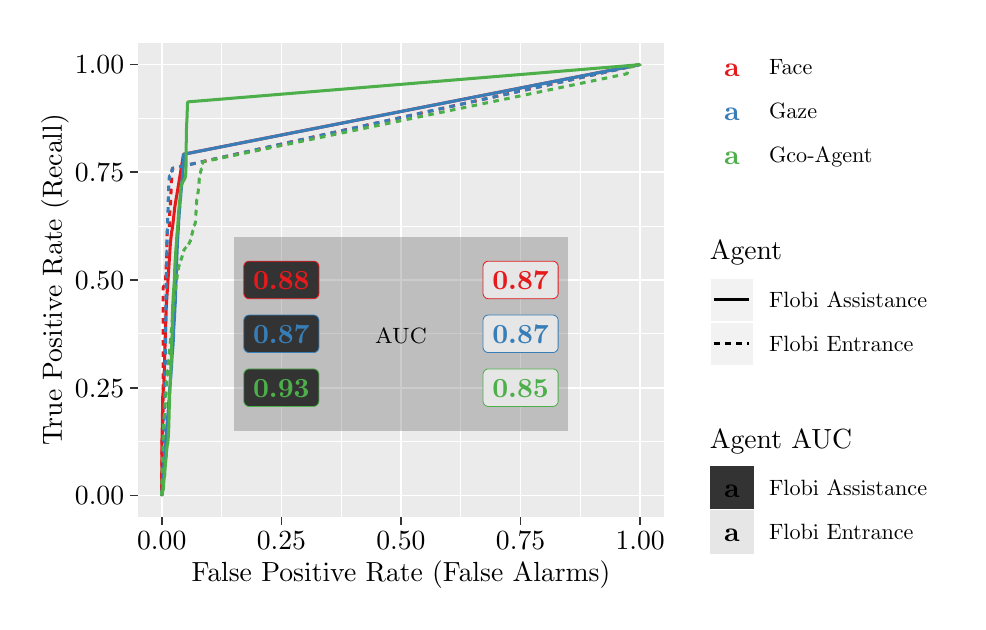
\begin{tikzpicture}[x=1pt,y=1pt]
\definecolor{fillColor}{RGB}{255,255,255}
\path[use as bounding box,fill=fillColor,fill opacity=0.00] (0,0) rectangle (336.00,207.65);
\begin{scope}
\path[clip] (  0.00,  0.00) rectangle (336.00,207.65);
\definecolor{drawColor}{RGB}{255,255,255}
\definecolor{fillColor}{RGB}{255,255,255}

\path[draw=drawColor,line width= 0.6pt,line join=round,line cap=round,fill=fillColor] (  0.00,  0.00) rectangle (336.00,207.65);
\end{scope}
\begin{scope}
\path[clip] ( 39.80, 30.86) rectangle (229.98,202.15);
\definecolor{fillColor}{gray}{0.92}

\path[fill=fillColor] ( 39.80, 30.86) rectangle (229.98,202.15);
\definecolor{drawColor}{RGB}{255,255,255}

\path[draw=drawColor,line width= 0.3pt,line join=round] ( 39.80, 58.09) --
	(229.98, 58.09);

\path[draw=drawColor,line width= 0.3pt,line join=round] ( 39.80, 97.03) --
	(229.98, 97.03);

\path[draw=drawColor,line width= 0.3pt,line join=round] ( 39.80,135.96) --
	(229.98,135.96);

\path[draw=drawColor,line width= 0.3pt,line join=round] ( 39.80,174.90) --
	(229.98,174.90);

\path[draw=drawColor,line width= 0.3pt,line join=round] ( 70.06, 30.86) --
	( 70.06,202.15);

\path[draw=drawColor,line width= 0.3pt,line join=round] (113.28, 30.86) --
	(113.28,202.15);

\path[draw=drawColor,line width= 0.3pt,line join=round] (156.50, 30.86) --
	(156.50,202.15);

\path[draw=drawColor,line width= 0.3pt,line join=round] (199.73, 30.86) --
	(199.73,202.15);

\path[draw=drawColor,line width= 0.6pt,line join=round] ( 39.80, 38.62) --
	(229.98, 38.62);

\path[draw=drawColor,line width= 0.6pt,line join=round] ( 39.80, 77.56) --
	(229.98, 77.56);

\path[draw=drawColor,line width= 0.6pt,line join=round] ( 39.80,116.49) --
	(229.98,116.49);

\path[draw=drawColor,line width= 0.6pt,line join=round] ( 39.80,155.43) --
	(229.98,155.43);

\path[draw=drawColor,line width= 0.6pt,line join=round] ( 39.80,194.36) --
	(229.98,194.36);

\path[draw=drawColor,line width= 0.6pt,line join=round] ( 48.45, 30.86) --
	( 48.45,202.15);

\path[draw=drawColor,line width= 0.6pt,line join=round] ( 91.67, 30.86) --
	( 91.67,202.15);

\path[draw=drawColor,line width= 0.6pt,line join=round] (134.89, 30.86) --
	(134.89,202.15);

\path[draw=drawColor,line width= 0.6pt,line join=round] (178.11, 30.86) --
	(178.11,202.15);

\path[draw=drawColor,line width= 0.6pt,line join=round] (221.34, 30.86) --
	(221.34,202.15);
\definecolor{fillColor}{RGB}{89,89,89}

\path[fill=fillColor,fill opacity=0.30] ( 74.38, 61.98) rectangle (195.40,132.07);
\definecolor{drawColor}{RGB}{0,0,0}

\node[text=drawColor,anchor=base,inner sep=0pt, outer sep=0pt, scale=  1.00] at (134.89, 93.57) {\footnotesize{AUC}};
\definecolor{drawColor}{RGB}{228,26,28}

\path[draw=drawColor,line width= 1.1pt,line join=round] ( 48.45, 43.79) --
	( 48.45, 42.26) --
	( 48.45, 42.21) --
	( 48.45, 38.85) --
	( 48.48, 54.59) --
	( 48.48, 54.58) --
	( 48.48, 54.57) --
	( 48.49, 55.86) --
	( 48.67, 64.63) --
	( 48.81, 74.44) --
	( 48.81, 74.42) --
	( 48.81, 74.41) --
	( 48.81, 74.40) --
	( 49.22, 78.94) --
	( 49.67, 94.25) --
	( 50.08,106.83) --
	( 50.10,107.16) --
	( 50.10,107.28) --
	( 50.64,115.42) --
	( 51.58,129.89) --
	( 52.05,134.13) --
	( 52.08,134.20) --
	( 52.16,134.36) --
	( 52.48,136.71) --
	( 53.13,142.60) --
	( 53.72,146.29) --
	( 53.78,146.50) --
	( 56.32,161.91) --
	(221.34,194.36);

\path[draw=drawColor,line width= 1.1pt,dash pattern=on 2pt off 2pt ,line join=round] ( 48.45, 40.61) --
	( 48.45, 39.36) --
	( 48.45, 39.13) --
	( 48.45, 38.79) --
	( 48.45, 47.20) --
	( 48.45, 47.18) --
	( 48.45, 47.11) --
	( 48.45, 46.05) --
	( 48.45, 44.62) --
	( 48.45, 41.40) --
	( 48.46, 48.87) --
	( 48.49, 48.87) --
	( 48.60, 59.53) --
	( 48.74, 61.41) --
	( 48.74, 61.10) --
	( 48.93, 68.40) --
	( 48.94,113.79) --
	( 49.13,114.14) --
	( 49.50,114.62) --
	( 49.65,114.66) --
	( 49.74,114.66) --
	( 49.80,115.92) --
	( 50.15,123.32) --
	( 50.39,134.15) --
	( 50.40,134.15) --
	( 50.46,134.15) --
	( 51.04,134.15) --
	( 51.08,134.17) --
	( 51.11,134.99) --
	( 51.23,136.28) --
	( 51.26,139.19) --
	( 51.28,139.19) --
	( 51.33,140.76) --
	( 51.37,142.87) --
	( 51.42,143.06) --
	( 51.51,143.06) --
	( 51.57,143.06) --
	( 51.66,145.23) --
	( 52.03,153.61) --
	( 52.29,156.79) --
	( 52.34,156.83) --
	(221.34,194.36);
\definecolor{drawColor}{RGB}{55,126,184}

\path[draw=drawColor,line width= 1.1pt,line join=round] ( 48.45, 38.65) --
	( 48.45, 38.66) --
	( 48.45, 38.70) --
	( 48.46, 38.71) --
	( 48.46, 38.74) --
	( 48.46, 38.76) --
	( 48.47, 38.78) --
	( 48.47, 38.81) --
	( 48.47, 38.82) --
	( 48.48, 38.84) --
	( 48.48, 38.86) --
	( 48.48, 38.91) --
	( 48.48, 38.93) --
	( 48.48, 38.97) --
	( 48.48, 39.00) --
	( 48.48, 39.02) --
	( 48.48, 39.04) --
	( 48.48, 39.07) --
	( 48.48, 39.09) --
	( 48.48, 39.12) --
	( 48.48, 39.14) --
	( 48.48, 39.16) --
	( 48.48, 39.19) --
	( 48.48, 39.22) --
	( 48.48, 39.23) --
	( 48.48, 39.26) --
	( 48.48, 39.28) --
	( 48.48, 39.31) --
	( 48.49, 39.33) --
	( 48.49, 39.35) --
	( 48.49, 39.38) --
	( 48.50, 39.39) --
	( 48.50, 39.41) --
	( 48.50, 39.44) --
	( 48.50, 39.46) --
	( 48.50, 39.49) --
	( 48.50, 39.51) --
	( 48.50, 39.54) --
	( 48.50, 39.56) --
	( 48.50, 39.59) --
	( 48.50, 39.62) --
	( 48.50, 39.64) --
	( 48.51, 39.66) --
	( 48.51, 39.69) --
	( 48.51, 39.72) --
	( 48.51, 39.75) --
	( 48.51, 39.77) --
	( 48.51, 39.80) --
	( 48.51, 39.83) --
	( 48.51, 39.85) --
	( 48.51, 39.88) --
	( 48.52, 39.89) --
	( 48.52, 39.92) --
	( 48.52, 39.95) --
	( 48.53, 39.96) --
	( 48.53, 39.99) --
	( 48.53, 40.02) --
	( 48.53, 40.04) --
	( 48.53, 40.08) --
	( 48.54, 40.10) --
	( 48.54, 40.12) --
	( 48.54, 40.15) --
	( 48.54, 40.17) --
	( 48.54, 40.19) --
	( 48.54, 40.23) --
	( 48.54, 40.26) --
	( 48.54, 40.28) --
	( 48.54, 40.31) --
	( 48.54, 40.35) --
	( 48.54, 40.37) --
	( 48.54, 40.39) --
	( 48.55, 40.41) --
	( 48.55, 40.44) --
	( 48.55, 40.46) --
	( 48.55, 40.50) --
	( 48.55, 40.53) --
	( 48.55, 40.54) --
	( 48.55, 40.58) --
	( 48.55, 40.61) --
	( 48.55, 40.63) --
	( 48.55, 40.66) --
	( 48.55, 40.69) --
	( 48.57, 40.72) --
	( 48.57, 40.74) --
	( 48.57, 40.77) --
	( 48.57, 40.79) --
	( 48.57, 40.81) --
	( 48.58, 40.83) --
	( 48.58, 40.85) --
	( 48.58, 40.88) --
	( 48.58, 40.90) --
	( 48.58, 40.92) --
	( 48.58, 40.95) --
	( 48.59, 40.96) --
	( 48.59, 40.99) --
	( 48.59, 41.01) --
	( 48.59, 41.04) --
	( 48.59, 41.07) --
	( 48.59, 41.08) --
	( 48.60, 41.11) --
	( 48.60, 41.13) --
	( 48.60, 41.15) --
	( 48.60, 41.17) --
	( 48.61, 41.19) --
	( 48.61, 41.21) --
	( 48.61, 41.23) --
	( 48.62, 41.25) --
	( 48.62, 41.28) --
	( 48.62, 41.30) --
	( 48.62, 41.33) --
	( 48.62, 41.35) --
	( 48.62, 41.38) --
	( 48.62, 41.40) --
	( 48.63, 41.42) --
	( 48.63, 41.45) --
	( 48.63, 41.46) --
	( 48.63, 41.49) --
	( 48.63, 41.51) --
	( 48.64, 41.53) --
	( 48.64, 41.56) --
	( 48.64, 41.58) --
	( 48.64, 41.61) --
	( 48.64, 41.63) --
	( 48.64, 41.65) --
	( 48.64, 41.68) --
	( 48.64, 41.70) --
	( 48.64, 41.72) --
	( 48.65, 41.75) --
	( 48.65, 41.77) --
	( 48.65, 41.80) --
	( 48.65, 41.85) --
	( 48.65, 41.88) --
	( 48.65, 41.90) --
	( 48.65, 41.93) --
	( 48.65, 41.95) --
	( 48.65, 41.99) --
	( 48.66, 42.00) --
	( 48.66, 42.03) --
	( 48.66, 42.05) --
	( 48.66, 42.07) --
	( 48.66, 42.11) --
	( 48.66, 42.13) --
	( 48.66, 42.15) --
	( 48.66, 42.18) --
	( 48.66, 42.22) --
	( 48.66, 42.24) --
	( 48.66, 42.26) --
	( 48.66, 42.30) --
	( 48.66, 42.33) --
	( 48.66, 42.35) --
	( 48.66, 42.38) --
	( 48.66, 42.40) --
	( 48.66, 42.42) --
	( 48.66, 42.45) --
	( 48.67, 42.46) --
	( 48.67, 42.49) --
	( 48.67, 42.50) --
	( 48.67, 42.53) --
	( 48.67, 42.57) --
	( 48.68, 42.58) --
	( 48.68, 42.61) --
	( 48.68, 42.63) --
	( 48.68, 42.64) --
	( 48.68, 42.68) --
	( 48.68, 42.70) --
	( 48.68, 42.73) --
	( 48.69, 42.75) --
	( 48.69, 42.77) --
	( 48.69, 42.80) --
	( 48.69, 42.82) --
	( 48.69, 42.84) --
	( 48.69, 42.87) --
	( 48.70, 42.89) --
	( 48.70, 42.91) --
	( 48.70, 42.94) --
	( 48.70, 42.96) --
	( 48.70, 42.99) --
	( 48.70, 43.01) --
	( 48.70, 43.03) --
	( 48.70, 43.05) --
	( 48.70, 43.07) --
	( 48.70, 43.10) --
	( 48.70, 43.13) --
	( 48.70, 43.16) --
	( 48.70, 43.18) --
	( 48.70, 43.21) --
	( 48.70, 43.23) --
	( 48.70, 43.26) --
	( 48.70, 43.30) --
	( 48.70, 43.33) --
	( 48.70, 43.35) --
	( 48.70, 43.37) --
	( 48.70, 43.40) --
	( 48.70, 43.42) --
	( 48.70, 43.45) --
	( 48.70, 43.48) --
	( 48.71, 43.49) --
	( 48.71, 43.52) --
	( 48.71, 43.55) --
	( 48.71, 43.57) --
	( 48.71, 43.60) --
	( 48.72, 43.61) --
	( 48.72, 43.63) --
	( 48.73, 43.64) --
	( 48.73, 43.66) --
	( 48.74, 43.68) --
	( 48.74, 43.70) --
	( 48.74, 43.72) --
	( 48.74, 43.75) --
	( 48.74, 43.76) --
	( 48.74, 43.81) --
	( 48.74, 43.84) --
	( 48.75, 43.86) --
	( 48.75, 43.88) --
	( 48.75, 43.91) --
	( 48.75, 43.93) --
	( 48.75, 43.95) --
	( 48.75, 43.98) --
	( 48.75, 44.00) --
	( 48.75, 44.02) --
	( 48.75, 44.05) --
	( 48.75, 44.07) --
	( 48.75, 44.10) --
	( 48.75, 44.12) --
	( 48.75, 44.15) --
	( 48.75, 44.17) --
	( 48.75, 44.19) --
	( 48.76, 44.21) --
	( 48.76, 44.23) --
	( 48.76, 44.25) --
	( 48.76, 44.28) --
	( 48.76, 44.30) --
	( 48.76, 44.33) --
	( 48.76, 44.35) --
	( 48.77, 44.37) --
	( 48.77, 44.40) --
	( 48.78, 44.41) --
	( 48.78, 44.44) --
	( 48.78, 44.46) --
	( 48.78, 44.48) --
	( 48.78, 44.50) --
	( 48.78, 44.52) --
	( 48.78, 44.56) --
	( 48.79, 44.58) --
	( 48.79, 44.61) --
	( 48.79, 44.64) --
	( 48.79, 44.65) --
	( 48.79, 44.67) --
	( 48.79, 44.71) --
	( 48.79, 44.74) --
	( 48.79, 44.76) --
	( 48.79, 44.79) --
	( 48.79, 44.81) --
	( 48.79, 44.83) --
	( 48.80, 44.86) --
	( 48.81, 44.87) --
	( 48.81, 44.90) --
	( 48.81, 44.91) --
	( 48.81, 44.94) --
	( 48.82, 44.96) --
	( 48.82, 44.99) --
	( 48.82, 45.02) --
	( 48.82, 45.05) --
	( 48.82, 45.08) --
	( 48.83, 45.10) --
	( 48.83, 45.12) --
	( 48.83, 45.14) --
	( 48.83, 45.17) --
	( 48.83, 45.19) --
	( 48.83, 45.21) --
	( 48.84, 45.23) --
	( 48.84, 45.27) --
	( 48.84, 45.29) --
	( 48.84, 45.33) --
	( 48.84, 45.35) --
	( 48.84, 45.37) --
	( 48.84, 45.40) --
	( 48.84, 45.44) --
	( 48.84, 45.45) --
	( 48.84, 45.48) --
	( 48.85, 45.50) --
	( 48.85, 45.52) --
	( 48.85, 45.55) --
	( 48.85, 45.57) --
	( 48.85, 45.59) --
	( 48.85, 45.63) --
	( 48.86, 45.64) --
	( 48.86, 45.67) --
	( 48.86, 45.69) --
	( 48.86, 45.71) --
	( 48.87, 45.72) --
	( 48.87, 45.75) --
	( 48.87, 45.77) --
	( 48.88, 45.79) --
	( 48.88, 45.80) --
	( 48.88, 45.82) --
	( 48.88, 45.85) --
	( 48.88, 45.87) --
	( 48.89, 45.90) --
	( 48.89, 45.93) --
	( 48.89, 45.96) --
	( 48.89, 45.98) --
	( 48.90, 46.01) --
	( 48.90, 46.03) --
	( 48.90, 46.06) --
	( 48.90, 46.09) --
	( 48.90, 46.12) --
	( 48.90, 46.14) --
	( 48.90, 46.17) --
	( 48.90, 46.19) --
	( 48.90, 46.21) --
	( 48.91, 46.23) --
	( 48.91, 46.25) --
	( 48.91, 46.27) --
	( 48.92, 46.28) --
	( 48.92, 46.31) --
	( 48.92, 46.33) --
	( 48.92, 46.36) --
	( 48.92, 46.39) --
	( 48.93, 46.40) --
	( 48.93, 46.44) --
	( 48.93, 46.47) --
	( 48.93, 46.50) --
	( 48.93, 46.52) --
	( 48.93, 46.55) --
	( 48.93, 46.57) --
	( 48.93, 46.59) --
	( 48.93, 46.61) --
	( 48.93, 46.63) --
	( 48.93, 46.67) --
	( 48.93, 46.69) --
	( 48.94, 46.71) --
	( 48.94, 46.74) --
	( 48.94, 46.77) --
	( 48.94, 46.79) --
	( 48.95, 46.81) --
	( 48.95, 46.83) --
	( 48.95, 46.86) --
	( 48.95, 46.88) --
	( 48.95, 46.91) --
	( 48.95, 46.93) --
	( 48.96, 46.96) --
	( 48.96, 47.00) --
	( 48.96, 47.01) --
	( 48.97, 47.03) --
	( 48.97, 47.05) --
	( 48.97, 47.08) --
	( 48.97, 47.11) --
	( 48.98, 47.13) --
	( 48.98, 47.16) --
	( 48.99, 47.18) --
	( 48.99, 47.20) --
	( 48.99, 47.23) --
	( 49.00, 47.24) --
	( 49.01, 47.24) --
	( 49.01, 47.27) --
	( 49.01, 47.28) --
	( 49.01, 47.32) --
	( 49.01, 47.36) --
	( 49.02, 47.38) --
	( 49.02, 47.40) --
	( 49.02, 47.43) --
	( 49.02, 47.45) --
	( 49.03, 47.47) --
	( 49.03, 47.49) --
	( 49.03, 47.52) --
	( 49.03, 47.55) --
	( 49.03, 47.58) --
	( 49.03, 47.61) --
	( 49.03, 47.63) --
	( 49.03, 47.66) --
	( 49.03, 47.69) --
	( 49.03, 47.72) --
	( 49.03, 47.74) --
	( 49.04, 47.76) --
	( 49.04, 47.78) --
	( 49.05, 47.80) --
	( 49.05, 47.82) --
	( 49.05, 47.85) --
	( 49.05, 47.86) --
	( 49.06, 47.89) --
	( 49.06, 47.91) --
	( 49.06, 47.93) --
	( 49.06, 47.95) --
	( 49.06, 47.98) --
	( 49.07, 48.00) --
	( 49.07, 48.02) --
	( 49.07, 48.05) --
	( 49.07, 48.08) --
	( 49.08, 48.09) --
	( 49.08, 48.12) --
	( 49.08, 48.15) --
	( 49.08, 48.17) --
	( 49.08, 48.20) --
	( 49.08, 48.22) --
	( 49.08, 48.24) --
	( 49.08, 48.27) --
	( 49.08, 48.29) --
	( 49.08, 48.31) --
	( 49.08, 48.33) --
	( 49.08, 48.35) --
	( 49.08, 48.38) --
	( 49.08, 48.40) --
	( 49.09, 48.42) --
	( 49.09, 48.45) --
	( 49.09, 48.47) --
	( 49.09, 48.49) --
	( 49.09, 48.51) --
	( 49.10, 48.53) --
	( 49.10, 48.55) --
	( 49.11, 48.58) --
	( 49.11, 48.63) --
	( 49.11, 48.66) --
	( 49.11, 48.69) --
	( 49.11, 48.71) --
	( 49.11, 48.74) --
	( 49.11, 48.77) --
	( 49.11, 48.79) --
	( 49.11, 48.82) --
	( 49.11, 48.85) --
	( 49.11, 48.87) --
	( 49.11, 48.89) --
	( 49.11, 48.92) --
	( 49.11, 48.94) --
	( 49.12, 48.96) --
	( 49.13, 48.98) --
	( 49.13, 49.00) --
	( 49.13, 49.02) --
	( 49.14, 49.04) --
	( 49.14, 49.06) --
	( 49.14, 49.08) --
	( 49.15, 49.10) --
	( 49.15, 49.13) --
	( 49.15, 49.16) --
	( 49.15, 49.18) --
	( 49.16, 49.20) --
	( 49.16, 49.22) --
	( 49.16, 49.23) --
	( 49.16, 49.26) --
	( 49.16, 49.28) --
	( 49.16, 49.31) --
	( 49.16, 49.34) --
	( 49.16, 49.36) --
	( 49.16, 49.39) --
	( 49.16, 49.42) --
	( 49.17, 49.43) --
	( 49.17, 49.46) --
	( 49.18, 49.47) --
	( 49.18, 49.50) --
	( 49.18, 49.52) --
	( 49.18, 49.54) --
	( 49.18, 49.57) --
	( 49.18, 49.60) --
	( 49.18, 49.62) --
	( 49.18, 49.65) --
	( 49.18, 49.67) --
	( 49.18, 49.69) --
	( 49.18, 49.73) --
	( 49.19, 49.74) --
	( 49.19, 49.76) --
	( 49.19, 49.79) --
	( 49.19, 49.81) --
	( 49.19, 49.84) --
	( 49.20, 49.85) --
	( 49.20, 49.88) --
	( 49.21, 49.88) --
	( 49.21, 49.91) --
	( 49.21, 49.93) --
	( 49.21, 49.96) --
	( 49.21, 49.99) --
	( 49.21, 50.01) --
	( 49.21, 50.04) --
	( 49.21, 50.06) --
	( 49.21, 50.08) --
	( 49.21, 50.11) --
	( 49.22, 50.15) --
	( 49.22, 50.17) --
	( 49.22, 50.19) --
	( 49.23, 50.21) --
	( 49.24, 50.23) --
	( 49.24, 50.27) --
	( 49.24, 50.28) --
	( 49.24, 50.31) --
	( 49.24, 50.33) --
	( 49.26, 50.34) --
	( 49.26, 50.36) --
	( 49.26, 50.38) --
	( 49.26, 50.42) --
	( 49.27, 50.43) --
	( 49.27, 50.46) --
	( 49.27, 50.49) --
	( 49.27, 50.51) --
	( 49.27, 50.54) --
	( 49.27, 50.56) --
	( 49.27, 50.58) --
	( 49.27, 50.61) --
	( 49.28, 50.62) --
	( 49.28, 50.65) --
	( 49.28, 50.68) --
	( 49.28, 50.70) --
	( 49.28, 50.73) --
	( 49.28, 50.75) --
	( 49.28, 50.77) --
	( 49.28, 50.80) --
	( 49.28, 50.82) --
	( 49.28, 50.85) --
	( 49.28, 50.88) --
	( 49.28, 50.90) --
	( 49.29, 50.92) --
	( 49.29, 50.94) --
	( 49.29, 50.96) --
	( 49.30, 50.98) --
	( 49.30, 51.00) --
	( 49.30, 51.03) --
	( 49.31, 51.03) --
	( 49.31, 51.06) --
	( 49.31, 51.07) --
	( 49.31, 51.10) --
	( 49.31, 51.12) --
	( 49.31, 51.16) --
	( 49.31, 51.19) --
	( 49.32, 51.20) --
	( 49.32, 51.23) --
	( 49.32, 51.24) --
	( 49.34, 51.25) --
	( 49.34, 51.27) --
	( 49.34, 51.30) --
	( 49.34, 51.33) --
	( 49.34, 51.35) --
	( 49.34, 51.37) --
	( 49.35, 51.38) --
	( 49.35, 51.41) --
	( 49.35, 51.43) --
	( 49.35, 51.46) --
	( 49.35, 51.47) --
	( 49.35, 51.49) --
	( 49.35, 51.52) --
	( 49.35, 51.54) --
	( 49.35, 51.57) --
	( 49.35, 51.60) --
	( 49.36, 51.61) --
	( 49.36, 51.64) --
	( 49.36, 51.68) --
	( 49.37, 51.69) --
	( 49.37, 51.72) --
	( 49.37, 51.75) --
	( 49.37, 51.78) --
	( 49.37, 51.80) --
	( 49.37, 51.83) --
	( 49.37, 51.86) --
	( 49.37, 51.88) --
	( 49.37, 51.91) --
	( 49.37, 51.92) --
	( 49.37, 51.95) --
	( 49.37, 51.98) --
	( 49.37, 52.00) --
	( 49.38, 52.02) --
	( 49.38, 52.04) --
	( 49.39, 52.06) --
	( 49.39, 52.08) --
	( 49.39, 52.11) --
	( 49.39, 52.13) --
	( 49.39, 52.15) --
	( 49.39, 52.17) --
	( 49.40, 52.19) --
	( 49.40, 52.22) --
	( 49.40, 52.25) --
	( 49.40, 52.26) --
	( 49.40, 52.29) --
	( 49.41, 52.30) --
	( 49.41, 52.32) --
	( 49.41, 52.34) --
	( 49.41, 52.37) --
	( 49.42, 52.38) --
	( 49.42, 52.41) --
	( 49.42, 52.44) --
	( 49.42, 52.46) --
	( 49.42, 52.48) --
	( 49.42, 52.51) --
	( 49.42, 52.53) --
	( 49.44, 52.54) --
	( 49.44, 52.57) --
	( 49.44, 52.59) --
	( 49.44, 52.61) --
	( 49.44, 52.63) --
	( 49.45, 52.64) --
	( 49.45, 52.68) --
	( 49.45, 52.71) --
	( 49.45, 52.73) --
	( 49.45, 52.75) --
	( 49.45, 52.77) --
	( 49.45, 52.80) --
	( 49.45, 52.83) --
	( 49.45, 52.87) --
	( 49.47, 52.87) --
	( 49.47, 52.90) --
	( 49.47, 52.92) --
	( 49.47, 52.95) --
	( 49.47, 52.98) --
	( 49.47, 53.00) --
	( 49.47, 53.03) --
	( 49.47, 53.06) --
	( 49.48, 53.07) --
	( 49.48, 53.10) --
	( 49.48, 53.12) --
	( 49.48, 53.14) --
	( 49.49, 53.16) --
	( 49.49, 53.18) --
	( 49.49, 53.22) --
	( 49.49, 53.25) --
	( 49.49, 53.26) --
	( 49.49, 53.29) --
	( 49.49, 53.32) --
	( 49.50, 53.34) --
	( 49.50, 53.37) --
	( 49.50, 53.39) --
	( 49.50, 53.41) --
	( 49.51, 53.42) --
	( 49.51, 53.45) --
	( 49.51, 53.48) --
	( 49.51, 53.51) --
	( 49.52, 53.52) --
	( 49.52, 53.54) --
	( 49.52, 53.56) --
	( 49.52, 53.59) --
	( 49.52, 53.61) --
	( 49.52, 53.64) --
	( 49.53, 53.66) --
	( 49.53, 53.69) --
	( 49.53, 53.72) --
	( 49.53, 53.75) --
	( 49.53, 53.77) --
	( 49.53, 53.79) --
	( 49.53, 53.83) --
	( 49.53, 53.85) --
	( 49.53, 53.87) --
	( 49.53, 53.90) --
	( 49.54, 53.91) --
	( 49.54, 53.94) --
	( 49.55, 53.95) --
	( 49.56, 53.96) --
	( 49.56, 53.98) --
	( 49.56, 54.02) --
	( 49.56, 54.04) --
	( 49.56, 54.06) --
	( 49.56, 54.09) --
	( 49.56, 54.10) --
	( 49.56, 54.14) --
	( 49.57, 54.16) --
	( 49.57, 54.18) --
	( 49.57, 54.20) --
	( 49.57, 54.22) --
	( 49.58, 54.25) --
	( 49.58, 54.28) --
	( 49.58, 54.31) --
	( 49.58, 54.33) --
	( 49.58, 54.36) --
	( 49.58, 54.39) --
	( 49.59, 54.41) --
	( 49.59, 54.43) --
	( 49.59, 54.45) --
	( 49.59, 54.48) --
	( 49.59, 54.51) --
	( 49.59, 54.53) --
	( 49.59, 54.56) --
	( 49.59, 54.58) --
	( 49.59, 54.60) --
	( 49.59, 54.63) --
	( 49.60, 54.64) --
	( 49.60, 54.66) --
	( 49.60, 54.68) --
	( 49.61, 54.70) --
	( 49.61, 54.71) --
	( 49.61, 54.74) --
	( 49.62, 54.76) --
	( 49.62, 54.79) --
	( 49.62, 54.81) --
	( 49.62, 54.83) --
	( 49.62, 54.85) --
	( 49.63, 54.86) --
	( 49.63, 54.89) --
	( 49.63, 54.91) --
	( 49.64, 54.93) --
	( 49.64, 54.95) --
	( 49.64, 54.98) --
	( 49.64, 55.01) --
	( 49.64, 55.03) --
	( 49.64, 55.06) --
	( 49.64, 55.08) --
	( 49.64, 55.10) --
	( 49.65, 55.12) --
	( 49.65, 55.15) --
	( 49.65, 55.17) --
	( 49.65, 55.19) --
	( 49.65, 55.21) --
	( 49.65, 55.24) --
	( 49.65, 55.27) --
	( 49.65, 55.30) --
	( 49.65, 55.32) --
	( 49.65, 55.35) --
	( 49.65, 55.37) --
	( 49.66, 55.39) --
	( 49.66, 55.41) --
	( 49.66, 55.44) --
	( 49.66, 55.46) --
	( 49.66, 55.49) --
	( 49.67, 55.51) --
	( 49.67, 55.52) --
	( 49.67, 55.55) --
	( 49.67, 55.58) --
	( 49.67, 55.60) --
	( 49.67, 55.63) --
	( 49.67, 55.67) --
	( 49.68, 55.70) --
	( 49.68, 55.72) --
	( 49.68, 55.75) --
	( 49.68, 55.77) --
	( 49.68, 55.79) --
	( 49.68, 55.82) --
	( 49.68, 55.86) --
	( 49.68, 55.89) --
	( 49.68, 55.91) --
	( 49.68, 55.94) --
	( 49.68, 55.96) --
	( 49.71, 55.96) --
	( 49.71, 55.98) --
	( 49.71, 56.01) --
	( 49.71, 56.03) --
	( 49.71, 56.05) --
	( 49.71, 56.07) --
	( 49.72, 56.09) --
	( 49.73, 56.11) --
	( 49.73, 56.13) --
	( 49.73, 56.17) --
	( 49.73, 56.21) --
	( 49.73, 56.22) --
	( 49.73, 56.25) --
	( 49.73, 56.28) --
	( 49.73, 56.30) --
	( 49.74, 56.32) --
	( 49.74, 56.35) --
	( 49.75, 56.37) --
	( 49.75, 56.40) --
	( 49.75, 56.42) --
	( 49.75, 56.44) --
	( 49.76, 56.46) --
	( 49.76, 56.48) --
	( 49.76, 56.50) --
	( 49.76, 56.53) --
	( 49.77, 56.55) --
	( 49.77, 56.58) --
	( 49.77, 56.60) --
	( 49.77, 56.62) --
	( 49.77, 56.66) --
	( 49.77, 56.68) --
	( 49.77, 56.70) --
	( 49.77, 56.73) --
	( 49.78, 56.74) --
	( 49.78, 56.77) --
	( 49.78, 56.78) --
	( 49.78, 56.81) --
	( 49.78, 56.83) --
	( 49.78, 56.86) --
	( 49.78, 56.90) --
	( 49.78, 56.93) --
	( 49.79, 56.94) --
	( 49.80, 56.95) --
	( 49.80, 56.97) --
	( 49.80, 57.00) --
	( 49.80, 57.04) --
	( 49.80, 57.06) --
	( 49.81, 57.08) --
	( 49.81, 57.10) --
	( 49.81, 57.12) --
	( 49.82, 57.14) --
	( 49.82, 57.17) --
	( 49.82, 57.20) --
	( 49.82, 57.22) --
	( 49.82, 57.24) --
	( 49.82, 57.27) --
	( 49.82, 57.30) --
	( 49.82, 57.33) --
	( 49.82, 57.36) --
	( 49.83, 57.39) --
	( 49.83, 57.40) --
	( 49.84, 57.43) --
	( 49.85, 57.44) --
	( 49.85, 57.47) --
	( 49.85, 57.49) --
	( 49.85, 57.51) --
	( 49.86, 57.53) --
	( 49.86, 57.56) --
	( 49.86, 57.58) --
	( 49.86, 57.61) --
	( 49.86, 57.63) --
	( 49.87, 57.66) --
	( 49.87, 57.68) --
	( 49.88, 57.69) --
	( 49.88, 57.71) --
	( 49.88, 57.75) --
	( 49.88, 57.78) --
	( 49.88, 57.80) --
	( 49.88, 57.83) --
	( 49.90, 57.84) --
	( 49.90, 57.85) --
	( 49.90, 57.89) --
	( 49.90, 57.92) --
	( 49.91, 57.94) --
	( 49.91, 57.99) --
	( 49.91, 58.01) --
	( 49.92, 58.02) --
	( 49.92, 58.04) --
	( 49.92, 58.06) --
	( 49.92, 58.08) --
	( 49.92, 58.11) --
	( 49.92, 58.13) --
	( 49.93, 58.15) --
	( 49.93, 58.17) --
	( 49.93, 58.20) --
	( 49.93, 58.23) --
	( 49.93, 58.26) --
	( 49.93, 58.28) --
	( 49.94, 58.30) --
	( 49.95, 58.31) --
	( 49.95, 58.35) --
	( 49.96, 58.36) --
	( 49.96, 58.39) --
	( 49.96, 58.42) --
	( 49.96, 58.44) --
	( 49.96, 58.47) --
	( 49.96, 58.49) --
	( 49.97, 58.51) --
	( 49.97, 58.54) --
	( 49.97, 58.56) --
	( 49.97, 58.59) --
	( 49.97, 58.62) --
	( 49.97, 58.65) --
	( 49.97, 58.67) --
	( 49.97, 58.70) --
	( 49.97, 58.73) --
	( 49.97, 58.75) --
	( 49.97, 58.78) --
	( 49.97, 58.81) --
	( 49.97, 58.84) --
	( 49.98, 58.85) --
	( 49.98, 58.88) --
	( 49.98, 58.91) --
	( 49.98, 58.93) --
	( 49.99, 58.94) --
	( 49.99, 58.99) --
	( 49.99, 59.01) --
	( 49.99, 59.04) --
	( 49.99, 59.08) --
	( 50.00, 59.08) --
	( 50.00, 59.11) --
	( 50.00, 59.13) --
	( 50.00, 59.16) --
	( 50.00, 59.19) --
	( 50.00, 59.21) --
	( 50.01, 59.22) --
	( 50.01, 59.25) --
	( 50.01, 59.28) --
	( 50.01, 59.31) --
	( 50.02, 59.32) --
	( 50.02, 59.34) --
	( 50.03, 59.35) --
	( 50.04, 59.37) --
	( 50.04, 59.39) --
	( 50.04, 59.42) --
	( 50.05, 59.43) --
	( 50.05, 59.46) --
	( 50.05, 59.49) --
	( 50.05, 59.50) --
	( 50.05, 59.54) --
	( 50.05, 59.57) --
	( 50.05, 59.59) --
	( 50.05, 59.62) --
	( 50.05, 59.64) --
	( 50.05, 59.67) --
	( 50.05, 59.70) --
	( 50.05, 59.73) --
	( 50.05, 59.76) --
	( 50.05, 59.78) --
	( 50.05, 59.81) --
	( 50.06, 59.82) --
	( 50.06, 59.85) --
	( 50.06, 59.88) --
	( 50.06, 59.90) --
	( 50.06, 59.92) --
	( 50.06, 59.95) --
	( 50.06, 59.97) --
	( 50.06, 60.00) --
	( 50.06, 60.03) --
	( 50.06, 60.06) --
	( 50.06, 60.09) --
	( 50.06, 60.11) --
	( 50.06, 60.15) --
	( 50.06, 60.17) --
	( 50.07, 60.19) --
	( 50.07, 60.22) --
	( 50.07, 60.26) --
	( 50.07, 60.28) --
	( 50.07, 60.30) --
	( 50.07, 60.32) --
	( 50.08, 60.34) --
	( 50.08, 60.37) --
	( 50.08, 60.39) --
	( 50.08, 60.42) --
	( 50.08, 60.44) --
	( 50.08, 60.47) --
	( 50.08, 60.50) --
	( 50.09, 60.51) --
	( 50.09, 60.53) --
	( 50.10, 60.55) --
	( 50.10, 60.57) --
	( 50.10, 60.60) --
	( 50.10, 60.61) --
	( 50.10, 60.65) --
	( 50.11, 60.67) --
	( 50.11, 60.69) --
	( 50.11, 60.72) --
	( 50.11, 60.75) --
	( 50.11, 60.78) --
	( 50.11, 60.80) --
	( 50.11, 60.84) --
	( 50.11, 60.87) --
	( 50.11, 60.90) --
	( 50.11, 60.92) --
	( 50.11, 60.95) --
	( 50.11, 60.97) --
	( 50.11, 60.99) --
	( 50.11, 61.01) --
	( 50.11, 61.03) --
	( 50.12, 61.05) --
	( 50.12, 61.08) --
	( 50.12, 61.11) --
	( 50.12, 61.14) --
	( 50.12, 61.17) --
	( 50.12, 61.19) --
	( 50.12, 61.22) --
	( 50.12, 61.26) --
	( 50.12, 61.29) --
	( 50.12, 61.31) --
	( 50.13, 61.33) --
	( 50.13, 61.36) --
	( 50.13, 61.38) --
	( 50.14, 61.40) --
	( 50.14, 61.42) --
	( 50.14, 61.45) --
	( 50.14, 61.47) --
	( 50.14, 61.50) --
	( 50.14, 61.53) --
	( 50.14, 61.55) --
	( 50.14, 61.57) --
	( 50.14, 61.61) --
	( 50.14, 61.63) --
	( 50.14, 61.65) --
	( 50.14, 61.68) --
	( 50.15, 61.70) --
	( 50.16, 61.71) --
	( 50.16, 61.75) --
	( 50.16, 61.77) --
	( 50.16, 61.80) --
	( 50.16, 61.84) --
	( 50.16, 61.87) --
	( 50.16, 61.89) --
	( 50.16, 61.91) --
	( 50.16, 61.94) --
	( 50.16, 61.96) --
	( 50.16, 61.99) --
	( 50.16, 62.01) --
	( 50.17, 62.03) --
	( 50.17, 62.06) --
	( 50.17, 62.08) --
	( 50.17, 62.11) --
	( 50.18, 62.13) --
	( 50.18, 62.14) --
	( 50.18, 62.17) --
	( 50.18, 62.19) --
	( 50.18, 62.22) --
	( 50.18, 62.24) --
	( 50.19, 62.26) --
	( 50.19, 62.29) --
	( 50.19, 62.31) --
	( 50.19, 62.34) --
	( 50.20, 62.36) --
	( 50.21, 62.37) --
	( 50.21, 62.41) --
	( 50.21, 62.43) --
	( 50.21, 62.45) --
	( 50.21, 62.47) --
	( 50.21, 62.49) --
	( 50.21, 62.52) --
	( 50.21, 62.54) --
	( 50.22, 62.56) --
	( 50.22, 62.58) --
	( 50.23, 62.60) --
	( 50.23, 62.62) --
	( 50.23, 62.64) --
	( 50.23, 62.66) --
	( 50.24, 62.68) --
	( 50.24, 62.71) --
	( 50.24, 62.73) --
	( 50.24, 62.76) --
	( 50.25, 62.78) --
	( 50.25, 62.80) --
	( 50.25, 62.83) --
	( 50.25, 62.88) --
	( 50.25, 62.91) --
	( 50.26, 62.93) --
	( 50.26, 62.95) --
	( 50.26, 62.98) --
	( 50.27, 62.99) --
	( 50.27, 63.00) --
	( 50.27, 63.02) --
	( 50.27, 63.05) --
	( 50.28, 63.07) --
	( 50.28, 63.10) --
	( 50.28, 63.13) --
	( 50.28, 63.14) --
	( 50.28, 63.17) --
	( 50.28, 63.19) --
	( 50.28, 63.22) --
	( 50.29, 63.23) --
	( 50.29, 63.25) --
	( 50.29, 63.27) --
	( 50.29, 63.29) --
	( 50.30, 63.32) --
	( 50.30, 63.36) --
	( 50.31, 63.39) --
	( 50.31, 63.41) --
	( 50.31, 63.43) --
	( 50.31, 63.45) --
	( 50.32, 63.46) --
	( 50.32, 63.49) --
	( 50.32, 63.52) --
	( 50.33, 63.55) --
	( 50.33, 63.57) --
	( 50.33, 63.60) --
	( 50.33, 63.64) --
	( 50.34, 63.65) --
	( 50.34, 63.68) --
	( 50.34, 63.71) --
	( 50.34, 63.74) --
	( 50.34, 63.77) --
	( 50.34, 63.79) --
	( 50.34, 63.82) --
	( 50.34, 63.83) --
	( 50.34, 63.87) --
	( 50.34, 63.89) --
	( 50.36, 63.91) --
	( 50.36, 63.92) --
	( 50.36, 63.95) --
	( 50.36, 63.98) --
	( 50.36, 64.00) --
	( 50.36, 64.02) --
	( 50.36, 64.05) --
	( 50.37, 64.06) --
	( 50.37, 64.09) --
	( 50.38, 64.10) --
	( 50.38, 64.14) --
	( 50.38, 64.17) --
	( 50.38, 64.20) --
	( 50.38, 64.21) --
	( 50.38, 64.24) --
	( 50.38, 64.26) --
	( 50.38, 64.30) --
	( 50.38, 64.33) --
	( 50.39, 64.34) --
	( 50.39, 64.37) --
	( 50.39, 64.40) --
	( 50.39, 64.42) --
	( 50.39, 64.44) --
	( 50.39, 64.48) --
	( 50.39, 64.50) --
	( 50.39, 64.52) --
	( 50.39, 64.55) --
	( 50.39, 64.57) --
	( 50.40, 64.59) --
	( 50.40, 64.61) --
	( 50.40, 64.63) --
	( 50.40, 64.67) --
	( 50.40, 64.70) --
	( 50.40, 64.73) --
	( 50.40, 64.75) --
	( 50.40, 64.78) --
	( 50.40, 64.80) --
	( 50.40, 64.83) --
	( 50.40, 64.86) --
	( 50.41, 64.88) --
	( 50.41, 64.90) --
	( 50.41, 64.93) --
	( 50.41, 64.96) --
	( 50.42, 64.97) --
	( 50.42, 64.99) --
	( 50.42, 65.02) --
	( 50.42, 65.05) --
	( 50.42, 65.08) --
	( 50.43, 65.09) --
	( 50.43, 65.12) --
	( 50.43, 65.15) --
	( 50.44, 65.17) --
	( 50.44, 65.19) --
	( 50.44, 65.21) --
	( 50.44, 65.23) --
	( 50.44, 65.25) --
	( 50.44, 65.29) --
	( 50.45, 65.30) --
	( 50.45, 65.32) --
	( 50.45, 65.35) --
	( 50.45, 65.39) --
	( 50.45, 65.41) --
	( 50.46, 65.43) --
	( 50.46, 65.44) --
	( 50.46, 65.48) --
	( 50.46, 65.52) --
	( 50.47, 65.53) --
	( 50.48, 65.55) --
	( 50.48, 65.58) --
	( 50.48, 65.60) --
	( 50.48, 65.63) --
	( 50.48, 65.66) --
	( 50.49, 65.67) --
	( 50.49, 65.71) --
	( 50.49, 65.73) --
	( 50.49, 65.75) --
	( 50.49, 65.78) --
	( 50.49, 65.82) --
	( 50.49, 65.86) --
	( 50.49, 65.88) --
	( 50.49, 65.91) --
	( 50.49, 65.93) --
	( 50.49, 65.95) --
	( 50.50, 65.97) --
	( 50.51, 65.98) --
	( 50.51, 66.01) --
	( 50.51, 66.05) --
	( 50.51, 66.07) --
	( 50.51, 66.09) --
	( 50.51, 66.12) --
	( 50.51, 66.14) --
	( 50.51, 66.18) --
	( 50.51, 66.20) --
	( 50.51, 66.24) --
	( 50.52, 66.25) --
	( 50.52, 66.27) --
	( 50.52, 66.29) --
	( 50.53, 66.31) --
	( 50.53, 66.32) --
	( 50.53, 66.35) --
	( 50.54, 66.36) --
	( 50.54, 66.39) --
	( 50.54, 66.41) --
	( 50.54, 66.43) --
	( 50.54, 66.46) --
	( 50.54, 66.47) --
	( 50.54, 66.51) --
	( 50.54, 66.53) --
	( 50.54, 66.55) --
	( 50.54, 66.59) --
	( 50.54, 66.63) --
	( 50.55, 66.65) --
	( 50.55, 66.67) --
	( 50.55, 66.70) --
	( 50.55, 66.73) --
	( 50.56, 66.75) --
	( 50.57, 66.77) --
	( 50.57, 66.81) --
	( 50.57, 66.83) --
	( 50.57, 66.86) --
	( 50.58, 66.88) --
	( 50.58, 66.91) --
	( 50.58, 66.93) --
	( 50.58, 66.96) --
	( 50.58, 66.98) --
	( 50.58, 67.00) --
	( 50.58, 67.02) --
	( 50.58, 67.05) --
	( 50.59, 67.06) --
	( 50.59, 67.08) --
	( 50.60, 67.09) --
	( 50.60, 67.12) --
	( 50.60, 67.15) --
	( 50.60, 67.17) --
	( 50.60, 67.20) --
	( 50.60, 67.22) --
	( 50.61, 67.24) --
	( 50.62, 67.27) --
	( 50.62, 67.29) --
	( 50.62, 67.31) --
	( 50.62, 67.33) --
	( 50.62, 67.36) --
	( 50.62, 67.39) --
	( 50.62, 67.41) --
	( 50.63, 67.43) --
	( 50.63, 67.44) --
	( 50.63, 67.47) --
	( 50.64, 67.47) --
	( 50.64, 67.50) --
	( 50.64, 67.52) --
	( 50.65, 67.54) --
	( 50.65, 67.55) --
	( 50.65, 67.58) --
	( 50.65, 67.60) --
	( 50.65, 67.64) --
	( 50.65, 67.68) --
	( 50.65, 67.70) --
	( 50.65, 67.73) --
	( 50.65, 67.75) --
	( 50.65, 67.78) --
	( 50.66, 67.79) --
	( 50.66, 67.82) --
	( 50.66, 67.85) --
	( 50.66, 67.87) --
	( 50.66, 67.89) --
	( 50.66, 67.93) --
	( 50.66, 67.98) --
	( 50.66, 68.01) --
	( 50.66, 68.04) --
	( 50.67, 68.05) --
	( 50.67, 68.08) --
	( 50.68, 68.09) --
	( 50.68, 68.12) --
	( 50.68, 68.15) --
	( 50.69, 68.16) --
	( 50.69, 68.18) --
	( 50.69, 68.20) --
	( 50.72, 68.22) --
	( 50.72, 68.24) --
	( 50.72, 68.27) --
	( 50.72, 68.29) --
	( 50.72, 68.31) --
	( 50.72, 68.34) --
	( 50.73, 68.35) --
	( 50.73, 68.37) --
	( 50.73, 68.39) --
	( 50.74, 68.40) --
	( 50.74, 68.43) --
	( 50.74, 68.46) --
	( 50.74, 68.49) --
	( 50.74, 68.51) --
	( 50.74, 68.54) --
	( 50.74, 68.58) --
	( 50.74, 68.59) --
	( 50.74, 68.62) --
	( 50.74, 68.65) --
	( 50.74, 68.67) --
	( 50.74, 68.69) --
	( 50.74, 68.72) --
	( 50.74, 68.74) --
	( 50.74, 68.77) --
	( 50.74, 68.80) --
	( 50.74, 68.82) --
	( 50.74, 68.85) --
	( 50.74, 68.88) --
	( 50.75, 68.89) --
	( 50.75, 68.91) --
	( 50.75, 68.93) --
	( 50.75, 68.96) --
	( 50.77, 68.97) --
	( 50.77, 69.00) --
	( 50.77, 69.02) --
	( 50.77, 69.05) --
	( 50.77, 69.08) --
	( 50.77, 69.10) --
	( 50.77, 69.12) --
	( 50.77, 69.14) --
	( 50.77, 69.16) --
	( 50.77, 69.19) --
	( 50.77, 69.22) --
	( 50.77, 69.24) --
	( 50.77, 69.27) --
	( 50.79, 69.29) --
	( 50.79, 69.32) --
	( 50.79, 69.34) --
	( 50.79, 69.36) --
	( 50.80, 69.37) --
	( 50.80, 69.39) --
	( 50.80, 69.42) --
	( 50.80, 69.45) --
	( 50.81, 69.46) --
	( 50.81, 69.50) --
	( 50.82, 69.52) --
	( 50.82, 69.54) --
	( 50.82, 69.58) --
	( 50.82, 69.60) --
	( 50.82, 69.62) --
	( 50.83, 69.64) --
	( 50.83, 69.66) --
	( 50.83, 69.69) --
	( 50.83, 69.71) --
	( 50.83, 69.73) --
	( 50.83, 69.76) --
	( 50.83, 69.77) --
	( 50.84, 69.80) --
	( 50.84, 69.81) --
	( 50.84, 69.84) --
	( 50.85, 69.86) --
	( 50.85, 69.88) --
	( 50.85, 69.91) --
	( 50.85, 69.94) --
	( 50.85, 69.96) --
	( 50.85, 69.99) --
	( 50.85, 70.01) --
	( 50.85, 70.04) --
	( 50.85, 70.06) --
	( 50.86, 70.07) --
	( 50.86, 70.11) --
	( 50.86, 70.13) --
	( 50.86, 70.15) --
	( 50.86, 70.18) --
	( 50.86, 70.20) --
	( 50.86, 70.23) --
	( 50.87, 70.25) --
	( 50.87, 70.27) --
	( 50.87, 70.30) --
	( 50.87, 70.33) --
	( 50.87, 70.37) --
	( 50.87, 70.41) --
	( 50.87, 70.43) --
	( 50.88, 70.44) --
	( 50.88, 70.46) --
	( 50.88, 70.49) --
	( 50.88, 70.52) --
	( 50.88, 70.54) --
	( 50.88, 70.57) --
	( 50.88, 70.60) --
	( 50.89, 70.61) --
	( 50.89, 70.65) --
	( 50.89, 70.66) --
	( 50.89, 70.69) --
	( 50.89, 70.73) --
	( 50.90, 70.75) --
	( 50.90, 70.76) --
	( 50.91, 70.78) --
	( 50.91, 70.80) --
	( 50.91, 70.83) --
	( 50.91, 70.85) --
	( 50.92, 70.88) --
	( 50.92, 70.90) --
	( 50.93, 70.92) --
	( 50.94, 70.93) --
	( 50.94, 70.96) --
	( 50.94, 70.99) --
	( 50.94, 71.01) --
	( 50.94, 71.04) --
	( 50.94, 71.07) --
	( 50.94, 71.09) --
	( 50.94, 71.11) --
	( 50.94, 71.14) --
	( 50.94, 71.16) --
	( 50.94, 71.18) --
	( 50.94, 71.22) --
	( 50.94, 71.25) --
	( 50.94, 71.27) --
	( 50.94, 71.30) --
	( 50.94, 71.34) --
	( 50.94, 71.36) --
	( 50.95, 71.38) --
	( 50.95, 71.40) --
	( 50.95, 71.43) --
	( 50.95, 71.45) --
	( 50.95, 71.48) --
	( 50.95, 71.51) --
	( 50.95, 71.53) --
	( 50.95, 71.56) --
	( 50.95, 71.58) --
	( 50.95, 71.61) --
	( 50.95, 71.63) --
	( 50.95, 71.66) --
	( 50.95, 71.68) --
	( 50.96, 71.70) --
	( 50.96, 71.73) --
	( 50.97, 71.75) --
	( 50.97, 71.78) --
	( 50.97, 71.80) --
	( 50.97, 71.83) --
	( 50.97, 71.84) --
	( 50.97, 71.87) --
	( 50.97, 71.90) --
	( 50.97, 71.92) --
	( 50.97, 71.95) --
	( 50.97, 71.98) --
	( 50.97, 72.00) --
	( 50.97, 72.03) --
	( 50.97, 72.05) --
	( 50.97, 72.07) --
	( 50.98, 72.09) --
	( 50.98, 72.11) --
	( 50.98, 72.13) --
	( 50.98, 72.15) --
	( 50.98, 72.18) --
	( 50.98, 72.20) --
	( 50.98, 72.22) --
	( 50.98, 72.26) --
	( 50.98, 72.28) --
	( 50.99, 72.30) --
	( 50.99, 72.32) --
	( 50.99, 72.34) --
	( 50.99, 72.37) --
	( 50.99, 72.39) --
	( 50.99, 72.42) --
	( 50.99, 72.44) --
	( 50.99, 72.47) --
	( 51.01, 72.48) --
	( 51.02, 72.49) --
	( 51.02, 72.51) --
	( 51.02, 72.53) --
	( 51.03, 72.55) --
	( 51.03, 72.57) --
	( 51.04, 72.59) --
	( 51.04, 72.60) --
	( 51.04, 72.63) --
	( 51.04, 72.65) --
	( 51.04, 72.68) --
	( 51.04, 72.71) --
	( 51.04, 72.73) --
	( 51.04, 72.76) --
	( 51.04, 72.79) --
	( 51.04, 72.81) --
	( 51.05, 72.83) --
	( 51.05, 72.84) --
	( 51.06, 72.87) --
	( 51.06, 72.90) --
	( 51.06, 72.92) --
	( 51.06, 72.95) --
	( 51.06, 72.99) --
	( 51.06, 73.01) --
	( 51.06, 73.03) --
	( 51.08, 73.05) --
	( 51.09, 73.06) --
	( 51.09, 73.09) --
	( 51.09, 73.11) --
	( 51.10, 73.12) --
	( 51.10, 73.14) --
	( 51.10, 73.16) --
	( 51.10, 73.18) --
	( 51.10, 73.21) --
	( 51.10, 73.23) --
	( 51.10, 73.26) --
	( 51.10, 73.29) --
	( 51.10, 73.31) --
	( 51.10, 73.33) --
	( 51.10, 73.36) --
	( 51.11, 73.37) --
	( 51.11, 73.40) --
	( 51.12, 73.41) --
	( 51.12, 73.45) --
	( 51.12, 73.48) --
	( 51.12, 73.51) --
	( 51.13, 73.52) --
	( 51.13, 73.55) --
	( 51.13, 73.56) --
	( 51.13, 73.60) --
	( 51.13, 73.62) --
	( 51.13, 73.64) --
	( 51.14, 73.66) --
	( 51.14, 73.68) --
	( 51.14, 73.71) --
	( 51.15, 73.73) --
	( 51.15, 73.75) --
	( 51.15, 73.77) --
	( 51.15, 73.79) --
	( 51.16, 73.82) --
	( 51.16, 73.85) --
	( 51.16, 73.87) --
	( 51.16, 73.91) --
	( 51.16, 73.94) --
	( 51.16, 73.96) --
	( 51.16, 73.98) --
	( 51.16, 74.01) --
	( 51.16, 74.04) --
	( 51.17, 74.06) --
	( 51.17, 74.08) --
	( 51.17, 74.10) --
	( 51.17, 74.13) --
	( 51.17, 74.16) --
	( 51.17, 74.18) --
	( 51.17, 74.21) --
	( 51.17, 74.24) --
	( 51.17, 74.26) --
	( 51.17, 74.29) --
	( 51.18, 74.30) --
	( 51.18, 74.33) --
	( 51.18, 74.35) --
	( 51.18, 74.36) --
	( 51.18, 74.39) --
	( 51.18, 74.41) --
	( 51.18, 74.45) --
	( 51.18, 74.48) --
	( 51.18, 74.51) --
	( 51.18, 74.53) --
	( 51.18, 74.56) --
	( 51.18, 74.59) --
	( 51.19, 74.60) --
	( 51.19, 74.63) --
	( 51.19, 74.65) --
	( 51.19, 74.67) --
	( 51.19, 74.71) --
	( 51.19, 74.73) --
	( 51.19, 74.75) --
	( 51.20, 74.76) --
	( 51.20, 74.79) --
	( 51.21, 74.80) --
	( 51.21, 74.83) --
	( 51.21, 74.86) --
	( 51.21, 74.89) --
	( 51.21, 74.90) --
	( 51.21, 74.94) --
	( 51.21, 74.96) --
	( 51.21, 74.98) --
	( 51.21, 75.01) --
	( 51.22, 75.02) --
	( 51.22, 75.05) --
	( 51.22, 75.07) --
	( 51.23, 75.10) --
	( 51.23, 75.13) --
	( 51.23, 75.15) --
	( 51.23, 75.18) --
	( 51.23, 75.21) --
	( 51.24, 75.22) --
	( 51.24, 75.25) --
	( 51.24, 75.28) --
	( 51.24, 75.31) --
	( 51.24, 75.33) --
	( 51.24, 75.36) --
	( 51.24, 75.38) --
	( 51.24, 75.40) --
	( 51.24, 75.43) --
	( 51.25, 75.44) --
	( 51.25, 75.47) --
	( 51.25, 75.50) --
	( 51.25, 75.52) --
	( 51.25, 75.55) --
	( 51.25, 75.57) --
	( 51.26, 75.59) --
	( 51.26, 75.62) --
	( 51.26, 75.64) --
	( 51.26, 75.67) --
	( 51.26, 75.69) --
	( 51.26, 75.72) --
	( 51.26, 75.74) --
	( 51.27, 75.76) --
	( 51.27, 75.78) --
	( 51.27, 75.81) --
	( 51.28, 75.82) --
	( 51.28, 75.84) --
	( 51.28, 75.86) --
	( 51.28, 75.90) --
	( 51.28, 75.92) --
	( 51.28, 75.94) --
	( 51.28, 75.97) --
	( 51.28, 75.99) --
	( 51.28, 76.02) --
	( 51.28, 76.05) --
	( 51.28, 76.08) --
	( 51.28, 76.11) --
	( 51.28, 76.13) --
	( 51.28, 76.16) --
	( 51.29, 76.19) --
	( 51.29, 76.21) --
	( 51.29, 76.24) --
	( 51.29, 76.27) --
	( 51.29, 76.29) --
	( 51.29, 76.32) --
	( 51.30, 76.33) --
	( 51.30, 76.36) --
	( 51.30, 76.39) --
	( 51.30, 76.41) --
	( 51.30, 76.44) --
	( 51.30, 76.46) --
	( 51.30, 76.48) --
	( 51.32, 76.49) --
	( 51.32, 76.51) --
	( 51.32, 76.54) --
	( 51.32, 76.56) --
	( 51.32, 76.59) --
	( 51.33, 76.60) --
	( 51.34, 76.62) --
	( 51.34, 76.64) --
	( 51.34, 76.67) --
	( 51.34, 76.71) --
	( 51.34, 76.74) --
	( 51.34, 76.77) --
	( 51.34, 76.79) --
	( 51.34, 76.82) --
	( 51.34, 76.85) --
	( 51.34, 76.89) --
	( 51.34, 76.92) --
	( 51.34, 76.95) --
	( 51.34, 76.97) --
	( 51.34, 77.00) --
	( 51.34, 77.02) --
	( 51.35, 77.05) --
	( 51.35, 77.08) --
	( 51.36, 77.09) --
	( 51.36, 77.12) --
	( 51.36, 77.13) --
	( 51.36, 77.16) --
	( 51.36, 77.18) --
	( 51.37, 77.20) --
	( 51.37, 77.22) --
	( 51.37, 77.24) --
	( 51.38, 77.28) --
	( 51.38, 77.30) --
	( 51.38, 77.33) --
	( 51.38, 77.35) --
	( 51.38, 77.37) --
	( 51.38, 77.40) --
	( 51.38, 77.43) --
	( 51.39, 77.45) --
	( 51.39, 77.47) --
	( 51.39, 77.50) --
	( 51.39, 77.53) --
	( 51.40, 77.54) --
	( 51.40, 77.56) --
	( 51.40, 77.59) --
	( 51.40, 77.62) --
	( 51.40, 77.64) --
	( 51.40, 77.66) --
	( 51.40, 77.69) --
	( 51.40, 77.71) --
	( 51.40, 77.74) --
	( 51.40, 77.77) --
	( 51.40, 77.80) --
	( 51.41, 77.81) --
	( 51.41, 77.85) --
	( 51.41, 77.88) --
	( 51.41, 77.90) --
	( 51.41, 77.92) --
	( 51.43, 77.93) --
	( 51.43, 77.95) --
	( 51.43, 77.97) --
	( 51.43, 78.00) --
	( 51.43, 78.02) --
	( 51.43, 78.04) --
	( 51.44, 78.06) --
	( 51.44, 78.08) --
	( 51.44, 78.12) --
	( 51.44, 78.14) --
	( 51.44, 78.16) --
	( 51.45, 78.17) --
	( 51.45, 78.19) --
	( 51.46, 78.20) --
	( 51.46, 78.23) --
	( 51.46, 78.24) --
	( 51.46, 78.27) --
	( 51.47, 78.28) --
	( 51.48, 78.31) --
	( 51.48, 78.34) --
	( 51.48, 78.36) --
	( 51.48, 78.39) --
	( 51.48, 78.41) --
	( 51.49, 78.43) --
	( 51.49, 78.46) --
	( 51.49, 78.49) --
	( 51.49, 78.50) --
	( 51.49, 78.54) --
	( 51.49, 78.56) --
	( 51.49, 78.58) --
	( 51.50, 78.60) --
	( 51.50, 78.62) --
	( 51.51, 78.64) --
	( 51.51, 78.66) --
	( 51.51, 78.69) --
	( 51.51, 78.72) --
	( 51.51, 78.74) --
	( 51.51, 78.77) --
	( 51.51, 78.80) --
	( 51.51, 78.81) --
	( 51.51, 78.85) --
	( 51.51, 78.88) --
	( 51.52, 78.89) --
	( 51.52, 78.91) --
	( 51.52, 78.93) --
	( 51.52, 78.96) --
	( 51.52, 78.98) --
	( 51.52, 79.00) --
	( 51.53, 79.02) --
	( 51.53, 79.04) --
	( 51.53, 79.07) --
	( 51.54, 79.08) --
	( 51.54, 79.11) --
	( 51.54, 79.13) --
	( 51.54, 79.15) --
	( 51.54, 79.18) --
	( 51.54, 79.20) --
	( 51.54, 79.23) --
	( 51.54, 79.25) --
	( 51.54, 79.27) --
	( 51.55, 79.28) --
	( 51.55, 79.31) --
	( 51.55, 79.35) --
	( 51.55, 79.38) --
	( 51.55, 79.42) --
	( 51.56, 79.43) --
	( 51.56, 79.46) --
	( 51.56, 79.50) --
	( 51.56, 79.52) --
	( 51.56, 79.54) --
	( 51.56, 79.57) --
	( 51.56, 79.59) --
	( 51.56, 79.61) --
	( 51.57, 79.63) --
	( 51.57, 79.65) --
	( 51.58, 79.66) --
	( 51.58, 79.69) --
	( 51.58, 79.71) --
	( 51.58, 79.73) --
	( 51.58, 79.77) --
	( 51.59, 79.79) --
	( 51.59, 79.81) --
	( 51.59, 79.84) --
	( 51.59, 79.87) --
	( 51.60, 79.89) --
	( 51.60, 79.92) --
	( 51.60, 79.94) --
	( 51.60, 79.96) --
	( 51.60, 79.99) --
	( 51.60, 80.01) --
	( 51.60, 80.03) --
	( 51.60, 80.06) --
	( 51.60, 80.08) --
	( 51.60, 80.10) --
	( 51.60, 80.12) --
	( 51.60, 80.15) --
	( 51.60, 80.17) --
	( 51.60, 80.19) --
	( 51.60, 80.22) --
	( 51.60, 80.25) --
	( 51.60, 80.28) --
	( 51.60, 80.31) --
	( 51.60, 80.34) --
	( 51.60, 80.36) --
	( 51.61, 80.38) --
	( 51.61, 80.40) --
	( 51.61, 80.43) --
	( 51.61, 80.46) --
	( 51.61, 80.48) --
	( 51.61, 80.50) --
	( 51.61, 80.52) --
	( 51.61, 80.55) --
	( 51.61, 80.57) --
	( 51.62, 80.60) --
	( 51.62, 80.62) --
	( 51.62, 80.65) --
	( 51.62, 80.68) --
	( 51.62, 80.69) --
	( 51.62, 80.72) --
	( 51.62, 80.75) --
	( 51.64, 80.76) --
	( 51.64, 80.78) --
	( 51.64, 80.80) --
	( 51.64, 80.84) --
	( 51.65, 80.85) --
	( 51.66, 80.88) --
	( 51.68, 80.88) --
	( 51.68, 80.91) --
	( 51.69, 80.93) --
	( 51.69, 80.95) --
	( 51.69, 80.98) --
	( 51.69, 81.00) --
	( 51.69, 81.03) --
	( 51.69, 81.07) --
	( 51.69, 81.09) --
	( 51.70, 81.11) --
	( 51.70, 81.14) --
	( 51.70, 81.17) --
	( 51.70, 81.19) --
	( 51.70, 81.22) --
	( 51.70, 81.25) --
	( 51.70, 81.27) --
	( 51.70, 81.30) --
	( 51.70, 81.34) --
	( 51.70, 81.35) --
	( 51.71, 81.37) --
	( 51.71, 81.39) --
	( 51.71, 81.41) --
	( 51.71, 81.44) --
	( 51.71, 81.46) --
	( 51.71, 81.49) --
	( 51.71, 81.52) --
	( 51.71, 81.54) --
	( 51.71, 81.57) --
	( 51.72, 81.59) --
	( 51.72, 81.61) --
	( 51.72, 81.64) --
	( 51.74, 81.65) --
	( 51.74, 81.68) --
	( 51.74, 81.70) --
	( 51.74, 81.72) --
	( 51.74, 81.76) --
	( 51.74, 81.77) --
	( 51.74, 81.80) --
	( 51.74, 81.83) --
	( 51.74, 81.85) --
	( 51.74, 81.87) --
	( 51.75, 81.90) --
	( 51.76, 81.92) --
	( 51.76, 81.95) --
	( 51.76, 81.97) --
	( 51.76, 81.99) --
	( 51.76, 82.01) --
	( 51.76, 82.05) --
	( 51.76, 82.08) --
	( 51.76, 82.10) --
	( 51.76, 82.13) --
	( 51.77, 82.15) --
	( 51.77, 82.18) --
	( 51.77, 82.20) --
	( 51.77, 82.22) --
	( 51.77, 82.25) --
	( 51.77, 82.27) --
	( 51.78, 82.29) --
	( 51.78, 82.32) --
	( 51.78, 82.34) --
	( 51.78, 82.37) --
	( 51.78, 82.39) --
	( 51.79, 82.40) --
	( 51.79, 82.43) --
	( 51.79, 82.45) --
	( 51.79, 82.49) --
	( 51.80, 82.51) --
	( 51.80, 82.53) --
	( 51.80, 82.56) --
	( 51.80, 82.59) --
	( 51.80, 82.61) --
	( 51.80, 82.64) --
	( 51.80, 82.66) --
	( 51.80, 82.69) --
	( 51.81, 82.70) --
	( 51.81, 82.72) --
	( 51.81, 82.75) --
	( 51.81, 82.77) --
	( 51.81, 82.79) --
	( 51.81, 82.83) --
	( 51.81, 82.85) --
	( 51.81, 82.87) --
	( 51.82, 82.89) --
	( 51.82, 82.91) --
	( 51.82, 82.94) --
	( 51.82, 82.96) --
	( 51.82, 82.98) --
	( 51.82, 83.01) --
	( 51.82, 83.03) --
	( 51.82, 83.05) --
	( 51.82, 83.07) --
	( 51.83, 83.10) --
	( 51.83, 83.12) --
	( 51.84, 83.14) --
	( 51.84, 83.17) --
	( 51.84, 83.19) --
	( 51.84, 83.21) --
	( 51.84, 83.24) --
	( 51.84, 83.25) --
	( 51.84, 83.28) --
	( 51.84, 83.30) --
	( 51.85, 83.32) --
	( 51.85, 83.34) --
	( 51.85, 83.37) --
	( 51.85, 83.39) --
	( 51.85, 83.41) --
	( 51.85, 83.44) --
	( 51.85, 83.47) --
	( 51.85, 83.49) --
	( 51.85, 83.52) --
	( 51.85, 83.54) --
	( 51.85, 83.56) --
	( 51.85, 83.60) --
	( 51.85, 83.63) --
	( 51.86, 83.64) --
	( 51.87, 83.66) --
	( 51.87, 83.69) --
	( 51.87, 83.71) --
	( 51.87, 83.73) --
	( 51.87, 83.76) --
	( 51.88, 83.79) --
	( 51.88, 83.81) --
	( 51.89, 83.83) --
	( 51.89, 83.86) --
	( 51.89, 83.88) --
	( 51.89, 83.90) --
	( 51.89, 83.94) --
	( 51.89, 83.97) --
	( 51.89, 83.98) --
	( 51.90, 84.01) --
	( 51.90, 84.03) --
	( 51.90, 84.06) --
	( 51.90, 84.09) --
	( 51.91, 84.10) --
	( 51.91, 84.12) --
	( 51.91, 84.15) --
	( 51.92, 84.17) --
	( 51.92, 84.19) --
	( 51.94, 84.20) --
	( 51.94, 84.23) --
	( 51.94, 84.25) --
	( 51.94, 84.28) --
	( 51.95, 84.29) --
	( 51.95, 84.31) --
	( 51.95, 84.33) --
	( 51.95, 84.36) --
	( 51.95, 84.40) --
	( 51.95, 84.42) --
	( 51.96, 84.43) --
	( 51.96, 84.46) --
	( 51.96, 84.50) --
	( 51.96, 84.52) --
	( 51.96, 84.55) --
	( 51.96, 84.57) --
	( 51.96, 84.60) --
	( 51.96, 84.63) --
	( 51.96, 84.64) --
	( 51.96, 84.68) --
	( 51.96, 84.71) --
	( 51.96, 84.74) --
	( 51.97, 84.75) --
	( 51.97, 84.78) --
	( 51.97, 84.80) --
	( 51.97, 84.82) --
	( 51.97, 84.86) --
	( 51.97, 84.88) --
	( 51.97, 84.90) --
	( 51.97, 84.94) --
	( 51.97, 84.98) --
	( 51.97, 84.99) --
	( 51.97, 85.01) --
	( 51.99, 85.02) --
	( 51.99, 85.05) --
	( 51.99, 85.09) --
	( 51.99, 85.12) --
	( 51.99, 85.14) --
	( 51.99, 85.17) --
	( 51.99, 85.20) --
	( 51.99, 85.22) --
	( 52.00, 85.28) --
	( 52.00, 85.31) --
	( 52.00, 85.33) --
	( 52.00, 85.36) --
	( 52.00, 85.38) --
	( 52.00, 85.40) --
	( 52.00, 85.43) --
	( 52.00, 85.45) --
	( 52.01, 85.47) --
	( 52.01, 85.50) --
	( 52.01, 85.52) --
	( 52.01, 85.56) --
	( 52.01, 85.58) --
	( 52.01, 85.60) --
	( 52.01, 85.63) --
	( 52.01, 85.65) --
	( 52.02, 85.67) --
	( 52.02, 85.70) --
	( 52.02, 85.72) --
	( 52.02, 85.76) --
	( 52.03, 85.78) --
	( 52.03, 85.81) --
	( 52.03, 85.84) --
	( 52.03, 85.86) --
	( 52.03, 85.90) --
	( 52.03, 85.92) --
	( 52.03, 85.94) --
	( 52.03, 85.97) --
	( 52.03, 85.99) --
	( 52.03, 86.01) --
	( 52.03, 86.05) --
	( 52.03, 86.08) --
	( 52.03, 86.10) --
	( 52.03, 86.13) --
	( 52.03, 86.15) --
	( 52.03, 86.18) --
	( 52.03, 86.20) --
	( 52.04, 86.22) --
	( 52.05, 86.23) --
	( 52.05, 86.25) --
	( 52.05, 86.28) --
	( 52.05, 86.31) --
	( 52.05, 86.34) --
	( 52.05, 86.36) --
	( 52.05, 86.39) --
	( 52.05, 86.43) --
	( 52.05, 86.45) --
	( 52.05, 86.47) --
	( 52.05, 86.50) --
	( 52.05, 86.52) --
	( 52.05, 86.55) --
	( 52.05, 86.58) --
	( 52.06, 86.59) --
	( 52.06, 86.62) --
	( 52.06, 86.64) --
	( 52.06, 86.66) --
	( 52.06, 86.69) --
	( 52.06, 86.71) --
	( 52.06, 86.74) --
	( 52.06, 86.76) --
	( 52.06, 86.78) --
	( 52.06, 86.80) --
	( 52.06, 86.83) --
	( 52.07, 86.85) --
	( 52.07, 86.87) --
	( 52.07, 86.89) --
	( 52.07, 86.91) --
	( 52.08, 86.93) --
	( 52.08, 86.96) --
	( 52.08, 86.98) --
	( 52.08, 87.01) --
	( 52.08, 87.03) --
	( 52.08, 87.05) --
	( 52.08, 87.08) --
	( 52.08, 87.11) --
	( 52.08, 87.15) --
	( 52.08, 87.17) --
	( 52.08, 87.20) --
	( 52.08, 87.23) --
	( 52.08, 87.25) --
	( 52.08, 87.28) --
	( 52.08, 87.31) --
	( 52.08, 87.33) --
	( 52.09, 87.35) --
	( 52.09, 87.38) --
	( 52.09, 87.40) --
	( 52.09, 87.43) --
	( 52.10, 87.45) --
	( 52.10, 87.47) --
	( 52.10, 87.50) --
	( 52.10, 87.52) --
	( 52.10, 87.55) --
	( 52.11, 87.57) --
	( 52.11, 87.59) --
	( 52.11, 87.61) --
	( 52.11, 87.63) --
	( 52.11, 87.66) --
	( 52.11, 87.69) --
	( 52.11, 87.72) --
	( 52.11, 87.74) --
	( 52.11, 87.77) --
	( 52.11, 87.79) --
	( 52.11, 87.81) --
	( 52.12, 87.83) --
	( 52.12, 87.85) --
	( 52.12, 87.88) --
	( 52.12, 87.90) --
	( 52.12, 87.93) --
	( 52.12, 87.94) --
	( 52.12, 87.96) --
	( 52.12, 87.99) --
	( 52.12, 88.02) --
	( 52.13, 88.04) --
	( 52.13, 88.06) --
	( 52.13, 88.08) --
	( 52.13, 88.10) --
	( 52.13, 88.14) --
	( 52.13, 88.16) --
	( 52.13, 88.19) --
	( 52.15, 88.21) --
	( 52.15, 88.23) --
	( 52.15, 88.26) --
	( 52.15, 88.29) --
	( 52.15, 88.31) --
	( 52.15, 88.34) --
	( 52.15, 88.37) --
	( 52.15, 88.39) --
	( 52.15, 88.41) --
	( 52.15, 88.43) --
	( 52.15, 88.46) --
	( 52.15, 88.48) --
	( 52.15, 88.50) --
	( 52.15, 88.53) --
	( 52.16, 88.55) --
	( 52.16, 88.58) --
	( 52.17, 88.59) --
	( 52.18, 88.61) --
	( 52.18, 88.64) --
	( 52.18, 88.66) --
	( 52.18, 88.69) --
	( 52.18, 88.72) --
	( 52.19, 88.74) --
	( 52.19, 88.77) --
	( 52.19, 88.81) --
	( 52.20, 88.83) --
	( 52.20, 88.85) --
	( 52.20, 88.87) --
	( 52.21, 88.88) --
	( 52.21, 88.90) --
	( 52.21, 88.92) --
	( 52.21, 88.95) --
	( 52.22, 88.96) --
	( 52.22, 88.99) --
	( 52.22, 89.03) --
	( 52.23, 89.05) --
	( 52.23, 89.09) --
	( 52.23, 89.11) --
	( 52.23, 89.14) --
	( 52.23, 89.16) --
	( 52.23, 89.19) --
	( 52.23, 89.23) --
	( 52.23, 89.25) --
	( 52.23, 89.28) --
	( 52.23, 89.31) --
	( 52.23, 89.34) --
	( 52.23, 89.37) --
	( 52.23, 89.39) --
	( 52.23, 89.42) --
	( 52.23, 89.46) --
	( 52.23, 89.50) --
	( 52.25, 89.50) --
	( 52.25, 89.53) --
	( 52.25, 89.55) --
	( 52.25, 89.57) --
	( 52.25, 89.60) --
	( 52.25, 89.62) --
	( 52.25, 89.65) --
	( 52.26, 89.66) --
	( 52.27, 89.68) --
	( 52.27, 89.70) --
	( 52.27, 89.73) --
	( 52.27, 89.76) --
	( 52.27, 89.78) --
	( 52.27, 89.80) --
	( 52.27, 89.83) --
	( 52.27, 89.85) --
	( 52.27, 89.88) --
	( 52.27, 89.90) --
	( 52.27, 89.92) --
	( 52.27, 89.96) --
	( 52.28, 89.97) --
	( 52.28, 90.00) --
	( 52.28, 90.03) --
	( 52.28, 90.04) --
	( 52.28, 90.08) --
	( 52.28, 90.11) --
	( 52.28, 90.14) --
	( 52.28, 90.16) --
	( 52.29, 90.18) --
	( 52.30, 90.20) --
	( 52.30, 90.23) --
	( 52.30, 90.26) --
	( 52.30, 90.29) --
	( 52.30, 90.32) --
	( 52.30, 90.35) --
	( 52.32, 90.35) --
	( 52.32, 90.38) --
	( 52.32, 90.40) --
	( 52.32, 90.42) --
	( 52.33, 90.44) --
	( 52.33, 90.46) --
	( 52.33, 90.49) --
	( 52.33, 90.51) --
	( 52.34, 90.53) --
	( 52.34, 90.56) --
	( 52.34, 90.58) --
	( 52.34, 90.61) --
	( 52.34, 90.64) --
	( 52.34, 90.66) --
	( 52.34, 90.69) --
	( 52.34, 90.72) --
	( 52.34, 90.75) --
	( 52.35, 90.77) --
	( 52.35, 90.79) --
	( 52.35, 90.81) --
	( 52.35, 90.84) --
	( 52.35, 90.86) --
	( 52.35, 90.90) --
	( 52.35, 90.92) --
	( 52.35, 90.95) --
	( 52.35, 90.97) --
	( 52.36, 90.99) --
	( 52.36, 91.02) --
	( 52.36, 91.05) --
	( 52.36, 91.07) --
	( 52.37, 91.08) --
	( 52.37, 91.11) --
	( 52.37, 91.14) --
	( 52.38, 91.16) --
	( 52.38, 91.18) --
	( 52.38, 91.22) --
	( 52.39, 91.23) --
	( 52.39, 91.26) --
	( 52.40, 91.27) --
	( 52.40, 91.31) --
	( 52.40, 91.34) --
	( 52.40, 91.36) --
	( 52.40, 91.38) --
	( 52.40, 91.41) --
	( 52.40, 91.43) --
	( 52.40, 91.45) --
	( 52.40, 91.48) --
	( 52.40, 91.50) --
	( 52.40, 91.53) --
	( 52.41, 91.55) --
	( 52.41, 91.57) --
	( 52.42, 91.58) --
	( 52.42, 91.60) --
	( 52.42, 91.62) --
	( 52.42, 91.64) --
	( 52.42, 91.67) --
	( 52.42, 91.69) --
	( 52.42, 91.72) --
	( 52.42, 91.75) --
	( 52.42, 91.77) --
	( 52.43, 91.79) --
	( 52.43, 91.83) --
	( 52.43, 91.86) --
	( 52.43, 91.89) --
	( 52.43, 91.91) --
	( 52.43, 91.95) --
	( 52.43, 91.97) --
	( 52.43, 91.99) --
	( 52.44, 92.01) --
	( 52.44, 92.03) --
	( 52.44, 92.06) --
	( 52.44, 92.08) --
	( 52.45, 92.10) --
	( 52.45, 92.12) --
	( 52.45, 92.15) --
	( 52.46, 92.17) --
	( 52.46, 92.18) --
	( 52.46, 92.21) --
	( 52.46, 92.23) --
	( 52.47, 92.25) --
	( 52.47, 92.27) --
	( 52.47, 92.29) --
	( 52.47, 92.31) --
	( 52.47, 92.34) --
	( 52.47, 92.37) --
	( 52.47, 92.40) --
	( 52.47, 92.42) --
	( 52.47, 92.45) --
	( 52.47, 92.48) --
	( 52.48, 92.50) --
	( 52.48, 92.52) --
	( 52.48, 92.55) --
	( 52.49, 92.56) --
	( 52.49, 92.60) --
	( 52.49, 92.61) --
	( 52.50, 92.63) --
	( 52.50, 92.66) --
	( 52.51, 92.68) --
	( 52.51, 92.71) --
	( 52.51, 92.73) --
	( 52.51, 92.76) --
	( 52.51, 92.78) --
	( 52.51, 92.80) --
	( 52.52, 92.82) --
	( 52.52, 92.85) --
	( 52.53, 92.87) --
	( 52.54, 92.88) --
	( 52.54, 92.91) --
	( 52.54, 92.93) --
	( 52.54, 92.96) --
	( 52.54, 92.98) --
	( 52.55, 93.00) --
	( 52.55, 93.02) --
	( 52.55, 93.06) --
	( 52.55, 93.08) --
	( 52.55, 93.10) --
	( 52.55, 93.14) --
	( 52.55, 93.17) --
	( 52.56, 93.18) --
	( 52.56, 93.21) --
	( 52.56, 93.24) --
	( 52.56, 93.26) --
	( 52.56, 93.29) --
	( 52.56, 93.33) --
	( 52.57, 93.34) --
	( 52.57, 93.37) --
	( 52.57, 93.39) --
	( 52.57, 93.42) --
	( 52.57, 93.44) --
	( 52.57, 93.46) --
	( 52.57, 93.48) --
	( 52.57, 93.51) --
	( 52.57, 93.54) --
	( 52.57, 93.56) --
	( 52.57, 93.60) --
	( 52.58, 93.62) --
	( 52.58, 93.64) --
	( 52.58, 93.67) --
	( 52.59, 93.70) --
	( 52.59, 93.72) --
	( 52.59, 93.75) --
	( 52.59, 93.79) --
	( 52.59, 93.81) --
	( 52.59, 93.84) --
	( 52.59, 93.87) --
	( 52.59, 93.90) --
	( 52.59, 93.92) --
	( 52.59, 93.95) --
	( 52.59, 93.98) --
	( 52.59, 94.02) --
	( 52.59, 94.04) --
	( 52.59, 94.06) --
	( 52.59, 94.09) --
	( 52.59, 94.11) --
	( 52.60, 94.13) --
	( 52.61, 94.14) --
	( 52.61, 94.17) --
	( 52.61, 94.19) --
	( 52.62, 94.21) --
	( 52.62, 94.24) --
	( 52.62, 94.26) --
	( 52.62, 94.29) --
	( 52.62, 94.31) --
	( 52.62, 94.33) --
	( 52.62, 94.36) --
	( 52.62, 94.38) --
	( 52.62, 94.40) --
	( 52.62, 94.43) --
	( 52.62, 94.45) --
	( 52.62, 94.48) --
	( 52.63, 94.49) --
	( 52.63, 94.54) --
	( 52.63, 94.56) --
	( 52.63, 94.59) --
	( 52.63, 94.63) --
	( 52.63, 94.65) --
	( 52.63, 94.67) --
	( 52.63, 94.70) --
	( 52.63, 94.71) --
	( 52.63, 94.74) --
	( 52.63, 94.78) --
	( 52.64, 94.79) --
	( 52.64, 94.82) --
	( 52.64, 94.85) --
	( 52.64, 94.87) --
	( 52.64, 94.90) --
	( 52.64, 94.93) --
	( 52.64, 94.95) --
	( 52.64, 94.97) --
	( 52.64, 94.99) --
	( 52.64, 95.01) --
	( 52.64, 95.05) --
	( 52.64, 95.08) --
	( 52.64, 95.10) --
	( 52.64, 95.14) --
	( 52.65, 95.16) --
	( 52.66, 95.17) --
	( 52.66, 95.20) --
	( 52.66, 95.22) --
	( 52.66, 95.24) --
	( 52.66, 95.26) --
	( 52.66, 95.28) --
	( 52.66, 95.32) --
	( 52.67, 95.32) --
	( 52.67, 95.36) --
	( 52.67, 95.38) --
	( 52.67, 95.41) --
	( 52.68, 95.44) --
	( 52.68, 95.47) --
	( 52.68, 95.50) --
	( 52.68, 95.52) --
	( 52.68, 95.55) --
	( 52.68, 95.58) --
	( 52.68, 95.59) --
	( 52.68, 95.62) --
	( 52.69, 95.63) --
	( 52.69, 95.67) --
	( 52.69, 95.70) --
	( 52.69, 95.72) --
	( 52.69, 95.75) --
	( 52.69, 95.78) --
	( 52.69, 95.80) --
	( 52.69, 95.82) --
	( 52.69, 95.85) --
	( 52.69, 95.87) --
	( 52.69, 95.89) --
	( 52.69, 95.92) --
	( 52.69, 95.94) --
	( 52.69, 95.97) --
	( 52.69, 95.99) --
	( 52.69, 96.01) --
	( 52.71, 96.03) --
	( 52.71, 96.05) --
	( 52.71, 96.08) --
	( 52.71, 96.10) --
	( 52.71, 96.13) --
	( 52.71, 96.16) --
	( 52.71, 96.19) --
	( 52.71, 96.22) --
	( 52.71, 96.24) --
	( 52.71, 96.28) --
	( 52.71, 96.31) --
	( 52.71, 96.34) --
	( 52.71, 96.36) --
	( 52.71, 96.40) --
	( 52.72, 96.41) --
	( 52.72, 96.44) --
	( 52.72, 96.47) --
	( 52.72, 96.49) --
	( 52.72, 96.51) --
	( 52.72, 96.53) --
	( 52.73, 96.55) --
	( 52.73, 96.58) --
	( 52.73, 96.61) --
	( 52.73, 96.64) --
	( 52.73, 96.66) --
	( 52.73, 96.70) --
	( 52.73, 96.72) --
	( 52.73, 96.75) --
	( 52.73, 96.78) --
	( 52.73, 96.81) --
	( 52.73, 96.84) --
	( 52.73, 96.86) --
	( 52.73, 96.88) --
	( 52.73, 96.90) --
	( 52.73, 96.93) --
	( 52.73, 96.95) --
	( 52.73, 96.98) --
	( 52.73, 97.01) --
	( 52.73, 97.03) --
	( 52.73, 97.06) --
	( 52.73, 97.09) --
	( 52.73, 97.12) --
	( 52.73, 97.14) --
	( 52.73, 97.16) --
	( 52.73, 97.19) --
	( 52.73, 97.22) --
	( 52.73, 97.24) --
	( 52.73, 97.27) --
	( 52.73, 97.30) --
	( 52.73, 97.32) --
	( 52.73, 97.35) --
	( 52.73, 97.39) --
	( 52.73, 97.41) --
	( 52.73, 97.43) --
	( 52.73, 97.46) --
	( 52.73, 97.49) --
	( 52.73, 97.51) --
	( 52.73, 97.54) --
	( 52.73, 97.56) --
	( 52.73, 97.58) --
	( 52.73, 97.62) --
	( 52.73, 97.64) --
	( 52.73, 97.66) --
	( 52.73, 97.69) --
	( 52.73, 97.71) --
	( 52.73, 97.73) --
	( 52.73, 97.76) --
	( 52.73, 97.78) --
	( 52.73, 97.81) --
	( 52.73, 97.85) --
	( 52.73, 97.87) --
	( 52.73, 97.89) --
	( 52.73, 97.92) --
	( 52.73, 97.96) --
	( 52.73, 97.98) --
	( 52.73, 98.01) --
	( 52.73, 98.04) --
	( 52.73, 98.07) --
	( 52.73, 98.10) --
	( 52.74, 98.11) --
	( 52.74, 98.13) --
	( 52.74, 98.16) --
	( 52.74, 98.19) --
	( 52.74, 98.21) --
	( 52.74, 98.24) --
	( 52.75, 98.26) --
	( 52.75, 98.28) --
	( 52.75, 98.31) --
	( 52.75, 98.34) --
	( 52.75, 98.36) --
	( 52.76, 98.38) --
	( 52.76, 98.40) --
	( 52.76, 98.42) --
	( 52.76, 98.44) --
	( 52.76, 98.46) --
	( 52.76, 98.50) --
	( 52.76, 98.54) --
	( 52.76, 98.56) --
	( 52.76, 98.60) --
	( 52.76, 98.63) --
	( 52.76, 98.65) --
	( 52.77, 98.67) --
	( 52.77, 98.70) --
	( 52.77, 98.73) --
	( 52.77, 98.74) --
	( 52.77, 98.77) --
	( 52.77, 98.79) --
	( 52.78, 98.81) --
	( 52.78, 98.84) --
	( 52.78, 98.87) --
	( 52.78, 98.89) --
	( 52.78, 98.92) --
	( 52.78, 98.93) --
	( 52.78, 98.96) --
	( 52.78, 98.98) --
	( 52.81, 98.99) --
	( 52.81, 99.01) --
	( 52.81, 99.04) --
	( 52.81, 99.07) --
	( 52.81, 99.09) --
	( 52.81, 99.12) --
	( 52.81, 99.15) --
	( 52.81, 99.17) --
	( 52.81, 99.20) --
	( 52.81, 99.23) --
	( 52.81, 99.27) --
	( 52.81, 99.30) --
	( 52.81, 99.32) --
	( 52.81, 99.34) --
	( 52.81, 99.38) --
	( 52.81, 99.40) --
	( 52.81, 99.42) --
	( 52.81, 99.46) --
	( 52.81, 99.50) --
	( 52.81, 99.51) --
	( 52.81, 99.54) --
	( 52.81, 99.57) --
	( 52.81, 99.59) --
	( 52.82, 99.61) --
	( 52.82, 99.64) --
	( 52.82, 99.66) --
	( 52.83, 99.69) --
	( 52.83, 99.71) --
	( 52.83, 99.73) --
	( 52.83, 99.76) --
	( 52.83, 99.79) --
	( 52.84, 99.80) --
	( 52.84, 99.83) --
	( 52.84, 99.87) --
	( 52.85, 99.88) --
	( 52.86, 99.89) --
	( 52.86, 99.92) --
	( 52.86, 99.94) --
	( 52.86, 99.96) --
	( 52.86, 99.99) --
	( 52.87,100.00) --
	( 52.87,100.03) --
	( 52.87,100.06) --
	( 52.87,100.09) --
	( 52.87,100.11) --
	( 52.87,100.13) --
	( 52.87,100.15) --
	( 52.87,100.19) --
	( 52.87,100.21) --
	( 52.87,100.23) --
	( 52.87,100.26) --
	( 52.87,100.28) --
	( 52.88,100.30) --
	( 52.88,100.31) --
	( 52.88,100.34) --
	( 52.88,100.38) --
	( 52.88,100.40) --
	( 52.88,100.42) --
	( 52.88,100.45) --
	( 52.89,100.47) --
	( 52.89,100.49) --
	( 52.90,100.52) --
	( 52.90,100.55) --
	( 52.90,100.57) --
	( 52.90,100.59) --
	( 52.91,100.61) --
	( 52.91,100.65) --
	( 52.91,100.67) --
	( 52.91,100.70) --
	( 52.92,100.72) --
	( 52.92,100.76) --
	( 52.93,100.78) --
	( 52.93,100.81) --
	( 52.93,100.84) --
	( 52.93,100.88) --
	( 52.93,100.91) --
	( 52.93,100.93) --
	( 52.93,100.95) --
	( 52.93,100.98) --
	( 52.93,101.01) --
	( 52.93,101.03) --
	( 52.93,101.05) --
	( 52.93,101.09) --
	( 52.94,101.11) --
	( 52.94,101.14) --
	( 52.94,101.17) --
	( 52.94,101.19) --
	( 52.94,101.22) --
	( 52.94,101.24) --
	( 52.94,101.26) --
	( 52.94,101.29) --
	( 52.94,101.32) --
	( 52.95,101.34) --
	( 52.95,101.37) --
	( 52.95,101.40) --
	( 52.95,101.42) --
	( 52.95,101.45) --
	( 52.95,101.46) --
	( 52.95,101.49) --
	( 52.97,101.52) --
	( 52.97,101.55) --
	( 52.97,101.57) --
	( 52.97,101.60) --
	( 52.97,101.63) --
	( 52.97,101.65) --
	( 52.97,101.68) --
	( 52.97,101.70) --
	( 52.97,101.72) --
	( 52.97,101.74) --
	( 52.97,101.77) --
	( 52.97,101.80) --
	( 52.97,101.83) --
	( 52.97,101.86) --
	( 52.98,101.89) --
	( 52.99,101.91) --
	( 52.99,101.93) --
	( 52.99,101.95) --
	( 52.99,101.97) --
	( 52.99,101.99) --
	( 53.00,102.02) --
	( 53.00,102.06) --
	( 53.00,102.08) --
	( 53.00,102.10) --
	( 53.00,102.12) --
	( 53.00,102.14) --
	( 53.00,102.17) --
	( 53.00,102.19) --
	( 53.00,102.22) --
	( 53.01,102.23) --
	( 53.01,102.25) --
	( 53.02,102.27) --
	( 53.02,102.30) --
	( 53.02,102.32) --
	( 53.02,102.34) --
	( 53.02,102.37) --
	( 53.03,102.39) --
	( 53.03,102.41) --
	( 53.03,102.45) --
	( 53.03,102.47) --
	( 53.03,102.52) --
	( 53.03,102.54) --
	( 53.03,102.57) --
	( 53.03,102.60) --
	( 53.04,102.62) --
	( 53.04,102.64) --
	( 53.04,102.67) --
	( 53.04,102.69) --
	( 53.04,102.73) --
	( 53.04,102.76) --
	( 53.04,102.79) --
	( 53.04,102.81) --
	( 53.05,102.83) --
	( 53.05,102.85) --
	( 53.05,102.87) --
	( 53.05,102.89) --
	( 53.05,102.91) --
	( 53.05,102.94) --
	( 53.05,102.97) --
	( 53.06,102.99) --
	( 53.06,103.02) --
	( 53.06,103.05) --
	( 53.06,103.08) --
	( 53.06,103.10) --
	( 53.07,103.12) --
	( 53.07,103.14) --
	( 53.07,103.17) --
	( 53.07,103.20) --
	( 53.07,103.22) --
	( 53.07,103.25) --
	( 53.07,103.29) --
	( 53.07,103.31) --
	( 53.07,103.33) --
	( 53.07,103.36) --
	( 53.07,103.39) --
	( 53.07,103.41) --
	( 53.07,103.44) --
	( 53.07,103.47) --
	( 53.07,103.51) --
	( 53.07,103.53) --
	( 53.07,103.56) --
	( 53.07,103.60) --
	( 53.07,103.62) --
	( 53.07,103.65) --
	( 53.07,103.67) --
	( 53.07,103.71) --
	( 53.08,103.73) --
	( 53.08,103.75) --
	( 53.08,103.78) --
	( 53.08,103.81) --
	( 53.08,103.83) --
	( 53.08,103.86) --
	( 53.08,103.88) --
	( 53.08,103.90) --
	( 53.08,103.93) --
	( 53.08,103.95) --
	( 53.09,103.96) --
	( 53.09,103.99) --
	( 53.09,104.02) --
	( 53.10,104.03) --
	( 53.10,104.06) --
	( 53.10,104.07) --
	( 53.10,104.10) --
	( 53.10,104.13) --
	( 53.10,104.17) --
	( 53.10,104.19) --
	( 53.10,104.21) --
	( 53.10,104.24) --
	( 53.10,104.27) --
	( 53.10,104.30) --
	( 53.10,104.33) --
	( 53.11,104.35) --
	( 53.11,104.37) --
	( 53.12,104.40) --
	( 53.12,104.42) --
	( 53.12,104.44) --
	( 53.12,104.48) --
	( 53.12,104.50) --
	( 53.12,104.52) --
	( 53.12,104.56) --
	( 53.12,104.58) --
	( 53.13,104.60) --
	( 53.13,104.63) --
	( 53.14,104.65) --
	( 53.14,104.67) --
	( 53.14,104.70) --
	( 53.14,104.72) --
	( 53.14,104.74) --
	( 53.14,104.77) --
	( 53.15,104.78) --
	( 53.15,104.80) --
	( 53.15,104.83) --
	( 53.15,104.86) --
	( 53.15,104.89) --
	( 53.15,104.91) --
	( 53.15,104.94) --
	( 53.15,104.97) --
	( 53.16,105.00) --
	( 53.16,105.03) --
	( 53.16,105.05) --
	( 53.16,105.08) --
	( 53.16,105.11) --
	( 53.16,105.13) --
	( 53.16,105.16) --
	( 53.16,105.18) --
	( 53.16,105.21) --
	( 53.16,105.24) --
	( 53.16,105.27) --
	( 53.16,105.29) --
	( 53.16,105.32) --
	( 53.16,105.34) --
	( 53.16,105.36) --
	( 53.16,105.39) --
	( 53.16,105.41) --
	( 53.16,105.43) --
	( 53.16,105.46) --
	( 53.17,105.47) --
	( 53.17,105.49) --
	( 53.17,105.51) --
	( 53.17,105.55) --
	( 53.17,105.59) --
	( 53.17,105.62) --
	( 53.17,105.65) --
	( 53.17,105.67) --
	( 53.17,105.70) --
	( 53.17,105.73) --
	( 53.17,105.75) --
	( 53.17,105.78) --
	( 53.17,105.81) --
	( 53.17,105.86) --
	( 53.17,105.89) --
	( 53.17,105.91) --
	( 53.17,105.93) --
	( 53.17,105.96) --
	( 53.17,105.98) --
	( 53.18,106.00) --
	( 53.18,106.02) --
	( 53.18,106.05) --
	( 53.18,106.07) --
	( 53.18,106.10) --
	( 53.18,106.12) --
	( 53.18,106.14) --
	( 53.19,106.16) --
	( 53.19,106.18) --
	( 53.19,106.20) --
	( 53.19,106.24) --
	( 53.19,106.27) --
	( 53.19,106.29) --
	( 53.19,106.32) --
	( 53.19,106.34) --
	( 53.19,106.36) --
	( 53.20,106.39) --
	( 53.20,106.42) --
	( 53.20,106.44) --
	( 53.20,106.47) --
	( 53.20,106.50) --
	( 53.20,106.53) --
	( 53.20,106.55) --
	( 53.22,106.56) --
	( 53.22,106.58) --
	( 53.23,106.60) --
	( 53.23,106.62) --
	( 53.23,106.66) --
	( 53.23,106.68) --
	( 53.23,106.70) --
	( 53.23,106.74) --
	( 53.23,106.76) --
	( 53.24,106.78) --
	( 53.24,106.80) --
	( 53.25,106.81) --
	( 53.25,106.83) --
	( 53.26,106.86) --
	( 53.26,106.89) --
	( 53.26,106.93) --
	( 53.26,106.97) --
	( 53.27,106.98) --
	( 53.27,107.00) --
	( 53.27,107.03) --
	( 53.27,107.06) --
	( 53.27,107.08) --
	( 53.27,107.11) --
	( 53.27,107.13) --
	( 53.27,107.16) --
	( 53.27,107.18) --
	( 53.27,107.21) --
	( 53.27,107.24) --
	( 53.27,107.27) --
	( 53.27,107.30) --
	( 53.27,107.33) --
	( 53.27,107.36) --
	( 53.27,107.39) --
	( 53.28,107.40) --
	( 53.28,107.42) --
	( 53.28,107.45) --
	( 53.28,107.48) --
	( 53.28,107.52) --
	( 53.28,107.54) --
	( 53.28,107.58) --
	( 53.28,107.61) --
	( 53.28,107.64) --
	( 53.28,107.66) --
	( 53.28,107.69) --
	( 53.29,107.70) --
	( 53.30,107.71) --
	( 53.30,107.73) --
	( 53.30,107.75) --
	( 53.30,107.78) --
	( 53.30,107.81) --
	( 53.30,107.85) --
	( 53.30,107.87) --
	( 53.30,107.89) --
	( 53.30,107.92) --
	( 53.31,107.94) --
	( 53.32,107.96) --
	( 53.32,107.98) --
	( 53.32,108.00) --
	( 53.33,108.01) --
	( 53.33,108.04) --
	( 53.33,108.08) --
	( 53.33,108.09) --
	( 53.34,108.11) --
	( 53.34,108.13) --
	( 53.34,108.15) --
	( 53.34,108.18) --
	( 53.34,108.21) --
	( 53.34,108.23) --
	( 53.34,108.26) --
	( 53.34,108.29) --
	( 53.34,108.31) --
	( 53.34,108.35) --
	( 53.34,108.37) --
	( 53.34,108.40) --
	( 53.34,108.42) --
	( 53.34,108.45) --
	( 53.34,108.47) --
	( 53.34,108.50) --
	( 53.34,108.53) --
	( 53.34,108.55) --
	( 53.34,108.58) --
	( 53.34,108.61) --
	( 53.34,108.65) --
	( 53.34,108.68) --
	( 53.34,108.71) --
	( 53.34,108.73) --
	( 53.35,108.75) --
	( 53.35,108.77) --
	( 53.35,108.80) --
	( 53.35,108.82) --
	( 53.35,108.84) --
	( 53.35,108.87) --
	( 53.36,108.88) --
	( 53.36,108.91) --
	( 53.36,108.93) --
	( 53.36,108.96) --
	( 53.36,108.99) --
	( 53.36,109.01) --
	( 53.36,109.04) --
	( 53.36,109.07) --
	( 53.36,109.10) --
	( 53.36,109.12) --
	( 53.36,109.15) --
	( 53.36,109.17) --
	( 53.36,109.20) --
	( 53.36,109.23) --
	( 53.37,109.24) --
	( 53.37,109.27) --
	( 53.37,109.29) --
	( 53.37,109.31) --
	( 53.37,109.34) --
	( 53.37,109.36) --
	( 53.38,109.38) --
	( 53.38,109.40) --
	( 53.38,109.42) --
	( 53.38,109.45) --
	( 53.39,109.46) --
	( 53.39,109.49) --
	( 53.39,109.52) --
	( 53.39,109.54) --
	( 53.39,109.57) --
	( 53.39,109.59) --
	( 53.39,109.62) --
	( 53.39,109.65) --
	( 53.39,109.67) --
	( 53.39,109.69) --
	( 53.40,109.73) --
	( 53.40,109.76) --
	( 53.40,109.79) --
	( 53.40,109.81) --
	( 53.40,109.84) --
	( 53.40,109.87) --
	( 53.40,109.89) --
	( 53.41,109.90) --
	( 53.41,109.93) --
	( 53.41,109.95) --
	( 53.43,109.96) --
	( 53.43,109.99) --
	( 53.43,110.01) --
	( 53.43,110.03) --
	( 53.43,110.06) --
	( 53.43,110.08) --
	( 53.43,110.11) --
	( 53.43,110.15) --
	( 53.43,110.18) --
	( 53.43,110.21) --
	( 53.43,110.23) --
	( 53.43,110.26) --
	( 53.44,110.28) --
	( 53.44,110.30) --
	( 53.44,110.34) --
	( 53.44,110.36) --
	( 53.44,110.38) --
	( 53.44,110.41) --
	( 53.44,110.43) --
	( 53.44,110.46) --
	( 53.44,110.50) --
	( 53.44,110.53) --
	( 53.45,110.54) --
	( 53.45,110.57) --
	( 53.45,110.59) --
	( 53.45,110.61) --
	( 53.45,110.63) --
	( 53.45,110.66) --
	( 53.45,110.68) --
	( 53.45,110.71) --
	( 53.45,110.74) --
	( 53.45,110.76) --
	( 53.45,110.80) --
	( 53.45,110.82) --
	( 53.46,110.85) --
	( 53.46,110.87) --
	( 53.46,110.91) --
	( 53.46,110.94) --
	( 53.46,110.95) --
	( 53.46,110.99) --
	( 53.46,111.01) --
	( 53.46,111.04) --
	( 53.47,111.06) --
	( 53.47,111.08) --
	( 53.47,111.10) --
	( 53.47,111.13) --
	( 53.47,111.15) --
	( 53.47,111.18) --
	( 53.47,111.21) --
	( 53.47,111.24) --
	( 53.47,111.26) --
	( 53.47,111.30) --
	( 53.48,111.31) --
	( 53.48,111.33) --
	( 53.48,111.36) --
	( 53.48,111.37) --
	( 53.48,111.41) --
	( 53.48,111.43) --
	( 53.48,111.46) --
	( 53.48,111.49) --
	( 53.48,111.52) --
	( 53.48,111.54) --
	( 53.48,111.56) --
	( 53.48,111.59) --
	( 53.48,111.62) --
	( 53.48,111.64) --
	( 53.48,111.67) --
	( 53.48,111.69) --
	( 53.48,111.72) --
	( 53.48,111.75) --
	( 53.48,111.78) --
	( 53.48,111.80) --
	( 53.48,111.83) --
	( 53.48,111.85) --
	( 53.48,111.87) --
	( 53.48,111.90) --
	( 53.48,111.92) --
	( 53.48,111.95) --
	( 53.48,111.99) --
	( 53.48,112.02) --
	( 53.48,112.05) --
	( 53.48,112.08) --
	( 53.48,112.10) --
	( 53.48,112.13) --
	( 53.48,112.15) --
	( 53.48,112.18) --
	( 53.48,112.20) --
	( 53.48,112.22) --
	( 53.48,112.25) --
	( 53.48,112.29) --
	( 53.48,112.33) --
	( 53.48,112.35) --
	( 53.48,112.37) --
	( 53.48,112.40) --
	( 53.48,112.44) --
	( 53.48,112.47) --
	( 53.48,112.49) --
	( 53.49,112.51) --
	( 53.49,112.55) --
	( 53.49,112.57) --
	( 53.49,112.60) --
	( 53.49,112.64) --
	( 53.49,112.67) --
	( 53.49,112.69) --
	( 53.49,112.72) --
	( 53.49,112.75) --
	( 53.49,112.78) --
	( 53.49,112.80) --
	( 53.49,112.83) --
	( 53.49,112.86) --
	( 53.49,112.88) --
	( 53.49,112.91) --
	( 53.49,112.94) --
	( 53.49,112.96) --
	( 53.50,112.98) --
	( 53.50,113.01) --
	( 53.50,113.03) --
	( 53.50,113.05) --
	( 53.50,113.08) --
	( 53.51,113.10) --
	( 53.51,113.11) --
	( 53.51,113.14) --
	( 53.51,113.17) --
	( 53.51,113.20) --
	( 53.51,113.22) --
	( 53.51,113.25) --
	( 53.51,113.27) --
	( 53.51,113.30) --
	( 53.51,113.33) --
	( 53.51,113.36) --
	( 53.52,113.37) --
	( 53.52,113.40) --
	( 53.52,113.43) --
	( 53.52,113.45) --
	( 53.53,113.47) --
	( 53.53,113.49) --
	( 53.53,113.52) --
	( 53.53,113.55) --
	( 53.53,113.57) --
	( 53.53,113.60) --
	( 53.53,113.63) --
	( 53.53,113.66) --
	( 53.53,113.67) --
	( 53.53,113.70) --
	( 53.53,113.74) --
	( 53.54,113.78) --
	( 53.54,113.81) --
	( 53.54,113.84) --
	( 53.54,113.86) --
	( 53.54,113.89) --
	( 53.54,113.90) --
	( 53.54,113.93) --
	( 53.54,113.96) --
	( 53.54,113.98) --
	( 53.54,114.01) --
	( 53.54,114.03) --
	( 53.55,114.05) --
	( 53.56,114.06) --
	( 53.56,114.09) --
	( 53.56,114.11) --
	( 53.56,114.13) --
	( 53.56,114.16) --
	( 53.56,114.18) --
	( 53.56,114.21) --
	( 53.56,114.23) --
	( 53.56,114.27) --
	( 53.56,114.30) --
	( 53.56,114.34) --
	( 53.56,114.36) --
	( 53.56,114.39) --
	( 53.56,114.41) --
	( 53.56,114.44) --
	( 53.56,114.46) --
	( 53.56,114.49) --
	( 53.56,114.51) --
	( 53.56,114.54) --
	( 53.56,114.56) --
	( 53.56,114.59) --
	( 53.56,114.63) --
	( 53.56,114.65) --
	( 53.56,114.68) --
	( 53.56,114.71) --
	( 53.56,114.74) --
	( 53.56,114.77) --
	( 53.56,114.79) --
	( 53.56,114.82) --
	( 53.56,114.84) --
	( 53.56,114.87) --
	( 53.56,114.90) --
	( 53.56,114.94) --
	( 53.58,114.95) --
	( 53.58,114.98) --
	( 53.58,115.01) --
	( 53.58,115.05) --
	( 53.58,115.09) --
	( 53.58,115.12) --
	( 53.58,115.14) --
	( 53.58,115.17) --
	( 53.58,115.20) --
	( 53.58,115.23) --
	( 53.58,115.25) --
	( 53.58,115.28) --
	( 53.58,115.29) --
	( 53.58,115.32) --
	( 53.58,115.34) --
	( 53.58,115.36) --
	( 53.58,115.39) --
	( 53.58,115.43) --
	( 53.58,115.45) --
	( 53.58,115.47) --
	( 53.58,115.50) --
	( 53.58,115.54) --
	( 53.59,115.55) --
	( 53.59,115.58) --
	( 53.59,115.60) --
	( 53.59,115.63) --
	( 53.59,115.66) --
	( 53.59,115.70) --
	( 53.59,115.72) --
	( 53.59,115.74) --
	( 53.59,115.76) --
	( 53.59,115.79) --
	( 53.60,115.81) --
	( 53.60,115.82) --
	( 53.60,115.85) --
	( 53.60,115.87) --
	( 53.60,115.89) --
	( 53.60,115.92) --
	( 53.60,115.95) --
	( 53.60,115.97) --
	( 53.60,116.01) --
	( 53.60,116.04) --
	( 53.61,116.05) --
	( 53.61,116.09) --
	( 53.61,116.12) --
	( 53.61,116.15) --
	( 53.61,116.17) --
	( 53.61,116.20) --
	( 53.61,116.23) --
	( 53.61,116.25) --
	( 53.61,116.28) --
	( 53.61,116.30) --
	( 53.61,116.31) --
	( 53.61,116.34) --
	( 53.61,116.37) --
	( 53.61,116.39) --
	( 53.61,116.42) --
	( 53.61,116.44) --
	( 53.62,116.46) --
	( 53.63,116.47) --
	( 53.63,116.50) --
	( 53.63,116.53) --
	( 53.63,116.56) --
	( 53.63,116.58) --
	( 53.63,116.61) --
	( 53.63,116.64) --
	( 53.63,116.66) --
	( 53.63,116.69) --
	( 53.63,116.72) --
	( 53.63,116.74) --
	( 53.63,116.77) --
	( 53.63,116.79) --
	( 53.64,116.81) --
	( 53.64,116.83) --
	( 53.64,116.85) --
	( 53.64,116.89) --
	( 53.64,116.92) --
	( 53.64,116.94) --
	( 53.64,116.96) --
	( 53.64,116.99) --
	( 53.64,117.01) --
	( 53.64,117.04) --
	( 53.65,117.06) --
	( 53.65,117.08) --
	( 53.65,117.11) --
	( 53.65,117.14) --
	( 53.65,117.16) --
	( 53.65,117.20) --
	( 53.65,117.22) --
	( 53.65,117.24) --
	( 53.65,117.27) --
	( 53.65,117.30) --
	( 53.65,117.33) --
	( 53.65,117.36) --
	( 53.66,117.39) --
	( 53.66,117.40) --
	( 53.66,117.43) --
	( 53.66,117.46) --
	( 53.66,117.48) --
	( 53.66,117.51) --
	( 53.66,117.54) --
	( 53.66,117.56) --
	( 53.66,117.58) --
	( 53.66,117.61) --
	( 53.66,117.64) --
	( 53.66,117.66) --
	( 53.66,117.69) --
	( 53.66,117.72) --
	( 53.66,117.74) --
	( 53.66,117.77) --
	( 53.67,117.81) --
	( 53.67,117.83) --
	( 53.68,117.85) --
	( 53.68,117.88) --
	( 53.68,117.90) --
	( 53.68,117.92) --
	( 53.68,117.96) --
	( 53.68,118.00) --
	( 53.68,118.02) --
	( 53.68,118.04) --
	( 53.68,118.08) --
	( 53.68,118.10) --
	( 53.68,118.12) --
	( 53.68,118.15) --
	( 53.68,118.18) --
	( 53.68,118.20) --
	( 53.68,118.23) --
	( 53.68,118.25) --
	( 53.68,118.27) --
	( 53.68,118.30) --
	( 53.68,118.31) --
	( 53.69,118.34) --
	( 53.69,118.37) --
	( 53.69,118.39) --
	( 53.69,118.42) --
	( 53.69,118.45) --
	( 53.69,118.47) --
	( 53.69,118.50) --
	( 53.69,118.52) --
	( 53.69,118.54) --
	( 53.69,118.57) --
	( 53.69,118.59) --
	( 53.69,118.61) --
	( 53.69,118.64) --
	( 53.69,118.67) --
	( 53.69,118.69) --
	( 53.69,118.72) --
	( 53.69,118.75) --
	( 53.69,118.77) --
	( 53.70,118.80) --
	( 53.70,118.83) --
	( 53.70,118.85) --
	( 53.71,118.87) --
	( 53.71,118.90) --
	( 53.71,118.94) --
	( 53.71,118.97) --
	( 53.71,119.00) --
	( 53.71,119.03) --
	( 53.71,119.07) --
	( 53.71,119.09) --
	( 53.71,119.12) --
	( 53.71,119.15) --
	( 53.71,119.16) --
	( 53.71,119.19) --
	( 53.71,119.21) --
	( 53.71,119.23) --
	( 53.71,119.26) --
	( 53.71,119.29) --
	( 53.71,119.31) --
	( 53.71,119.34) --
	( 53.71,119.36) --
	( 53.71,119.38) --
	( 53.71,119.42) --
	( 53.71,119.44) --
	( 53.71,119.46) --
	( 53.71,119.49) --
	( 53.71,119.53) --
	( 53.71,119.57) --
	( 53.71,119.60) --
	( 53.71,119.62) --
	( 53.71,119.65) --
	( 53.72,119.66) --
	( 53.72,119.69) --
	( 53.72,119.72) --
	( 53.72,119.75) --
	( 53.72,119.78) --
	( 53.72,119.81) --
	( 53.72,119.84) --
	( 53.72,119.87) --
	( 53.73,119.88) --
	( 53.73,119.91) --
	( 53.74,119.92) --
	( 53.74,119.95) --
	( 53.74,119.99) --
	( 53.74,120.02) --
	( 53.74,120.04) --
	( 53.74,120.06) --
	( 53.74,120.08) --
	( 53.74,120.11) --
	( 53.74,120.14) --
	( 53.74,120.16) --
	( 53.74,120.18) --
	( 53.74,120.21) --
	( 53.74,120.23) --
	( 53.74,120.26) --
	( 53.75,120.28) --
	( 53.75,120.30) --
	( 53.75,120.34) --
	( 53.75,120.37) --
	( 53.75,120.38) --
	( 53.75,120.41) --
	( 53.75,120.43) --
	( 53.75,120.45) --
	( 53.75,120.49) --
	( 53.76,120.50) --
	( 53.76,120.52) --
	( 53.76,120.54) --
	( 53.76,120.57) --
	( 53.76,120.59) --
	( 53.76,120.61) --
	( 53.76,120.64) --
	( 53.76,120.68) --
	( 53.76,120.70) --
	( 53.76,120.73) --
	( 53.76,120.76) --
	( 53.76,120.79) --
	( 53.76,120.81) --
	( 53.76,120.84) --
	( 53.77,120.86) --
	( 53.77,120.88) --
	( 53.77,120.91) --
	( 53.77,120.93) --
	( 53.78,120.95) --
	( 53.78,120.97) --
	( 53.78,120.99) --
	( 53.78,121.02) --
	( 53.78,121.04) --
	( 53.78,121.06) --
	( 53.78,121.10) --
	( 53.78,121.12) --
	( 53.78,121.14) --
	( 53.78,121.17) --
	( 53.78,121.20) --
	( 53.78,121.23) --
	( 53.78,121.26) --
	( 53.78,121.29) --
	( 53.78,121.31) --
	( 53.79,121.33) --
	( 53.79,121.35) --
	( 53.79,121.37) --
	( 53.79,121.40) --
	( 53.79,121.43) --
	( 53.79,121.45) --
	( 53.79,121.48) --
	( 53.79,121.51) --
	( 53.79,121.53) --
	( 53.79,121.55) --
	( 53.79,121.58) --
	( 53.79,121.61) --
	( 53.79,121.64) --
	( 53.79,121.66) --
	( 53.79,121.68) --
	( 53.80,121.70) --
	( 53.80,121.72) --
	( 53.80,121.75) --
	( 53.81,121.76) --
	( 53.81,121.79) --
	( 53.81,121.81) --
	( 53.81,121.83) --
	( 53.81,121.86) --
	( 53.81,121.88) --
	( 53.81,121.91) --
	( 53.81,121.94) --
	( 53.81,121.96) --
	( 53.81,121.98) --
	( 53.81,122.01) --
	( 53.81,122.04) --
	( 53.81,122.06) --
	( 53.81,122.09) --
	( 53.81,122.11) --
	( 53.81,122.14) --
	( 53.81,122.17) --
	( 53.81,122.19) --
	( 53.81,122.22) --
	( 53.81,122.25) --
	( 53.81,122.27) --
	( 53.82,122.29) --
	( 53.82,122.32) --
	( 53.82,122.35) --
	( 53.82,122.37) --
	( 53.82,122.40) --
	( 53.82,122.42) --
	( 53.82,122.44) --
	( 53.82,122.47) --
	( 53.82,122.49) --
	( 53.82,122.52) --
	( 53.82,122.56) --
	( 53.82,122.58) --
	( 53.82,122.60) --
	( 53.82,122.63) --
	( 53.82,122.65) --
	( 53.82,122.67) --
	( 53.82,122.71) --
	( 53.82,122.73) --
	( 53.82,122.75) --
	( 53.82,122.78) --
	( 53.82,122.80) --
	( 53.83,122.82) --
	( 53.83,122.84) --
	( 53.83,122.88) --
	( 53.83,122.90) --
	( 53.84,122.93) --
	( 53.84,122.96) --
	( 53.84,122.98) --
	( 53.84,123.01) --
	( 53.84,123.03) --
	( 53.84,123.06) --
	( 53.84,123.09) --
	( 53.84,123.11) --
	( 53.84,123.14) --
	( 53.84,123.17) --
	( 53.84,123.20) --
	( 53.84,123.22) --
	( 53.84,123.25) --
	( 53.85,123.26) --
	( 53.85,123.29) --
	( 53.85,123.31) --
	( 53.85,123.33) --
	( 53.85,123.36) --
	( 53.85,123.39) --
	( 53.85,123.43) --
	( 53.85,123.46) --
	( 53.85,123.48) --
	( 53.85,123.52) --
	( 53.85,123.54) --
	( 53.85,123.56) --
	( 53.85,123.59) --
	( 53.86,123.60) --
	( 53.87,123.63) --
	( 53.87,123.65) --
	( 53.87,123.67) --
	( 53.87,123.71) --
	( 53.87,123.74) --
	( 53.87,123.77) --
	( 53.88,123.78) --
	( 53.88,123.80) --
	( 53.88,123.82) --
	( 53.88,123.86) --
	( 53.88,123.88) --
	( 53.89,123.90) --
	( 53.89,123.91) --
	( 53.89,123.94) --
	( 53.89,123.96) --
	( 53.89,124.00) --
	( 53.89,124.04) --
	( 53.89,124.06) --
	( 53.89,124.09) --
	( 53.89,124.11) --
	( 53.89,124.14) --
	( 53.89,124.17) --
	( 53.89,124.21) --
	( 53.89,124.24) --
	( 53.89,124.26) --
	( 53.89,124.28) --
	( 53.89,124.31) --
	( 53.89,124.34) --
	( 53.89,124.37) --
	( 53.89,124.40) --
	( 53.90,124.43) --
	( 53.90,124.46) --
	( 53.90,124.49) --
	( 53.90,124.53) --
	( 53.90,124.55) --
	( 53.90,124.58) --
	( 53.90,124.60) --
	( 53.90,124.63) --
	( 53.90,124.66) --
	( 53.90,124.68) --
	( 53.90,124.70) --
	( 53.90,124.73) --
	( 53.90,124.75) --
	( 53.91,124.78) --
	( 53.91,124.80) --
	( 53.91,124.82) --
	( 53.91,124.85) --
	( 53.91,124.87) --
	( 53.91,124.90) --
	( 53.91,124.93) --
	( 53.91,124.95) --
	( 53.91,124.97) --
	( 53.91,125.00) --
	( 53.91,125.02) --
	( 53.91,125.05) --
	( 53.91,125.08) --
	( 53.91,125.10) --
	( 53.91,125.13) --
	( 53.92,125.14) --
	( 53.93,125.16) --
	( 53.93,125.20) --
	( 53.93,125.22) --
	( 53.93,125.24) --
	( 53.93,125.27) --
	( 53.93,125.30) --
	( 53.93,125.34) --
	( 53.93,125.36) --
	( 53.93,125.39) --
	( 53.93,125.41) --
	( 53.93,125.43) --
	( 53.93,125.46) --
	( 53.93,125.50) --
	( 53.93,125.53) --
	( 53.93,125.56) --
	( 53.93,125.59) --
	( 53.93,125.61) --
	( 53.93,125.63) --
	( 53.93,125.66) --
	( 53.93,125.69) --
	( 53.93,125.72) --
	( 53.93,125.75) --
	( 53.94,125.78) --
	( 53.94,125.79) --
	( 53.95,125.81) --
	( 53.95,125.83) --
	( 53.95,125.85) --
	( 53.95,125.87) --
	( 53.95,125.90) --
	( 53.95,125.93) --
	( 53.95,125.95) --
	( 53.95,125.98) --
	( 53.95,126.01) --
	( 53.96,126.03) --
	( 53.96,126.05) --
	( 53.96,126.07) --
	( 53.96,126.09) --
	( 53.96,126.12) --
	( 53.96,126.14) --
	( 53.96,126.17) --
	( 53.96,126.20) --
	( 53.96,126.23) --
	( 53.96,126.25) --
	( 53.96,126.27) --
	( 53.97,126.30) --
	( 53.97,126.32) --
	( 53.97,126.34) --
	( 53.97,126.36) --
	( 53.97,126.39) --
	( 53.97,126.41) --
	( 53.97,126.43) --
	( 53.97,126.47) --
	( 53.97,126.49) --
	( 53.97,126.52) --
	( 53.97,126.55) --
	( 53.97,126.58) --
	( 53.97,126.61) --
	( 53.97,126.63) --
	( 53.97,126.66) --
	( 53.97,126.68) --
	( 53.98,126.70) --
	( 53.98,126.72) --
	( 53.98,126.75) --
	( 53.98,126.77) --
	( 53.99,126.79) --
	( 53.99,126.82) --
	( 53.99,126.85) --
	( 53.99,126.88) --
	( 53.99,126.90) --
	( 53.99,126.93) --
	( 53.99,126.96) --
	( 53.99,126.99) --
	( 53.99,127.02) --
	( 53.99,127.05) --
	( 53.99,127.07) --
	( 53.99,127.09) --
	( 53.99,127.12) --
	( 54.00,127.14) --
	( 54.00,127.16) --
	( 54.00,127.19) --
	( 54.00,127.21) --
	( 54.00,127.23) --
	( 54.00,127.26) --
	( 54.00,127.29) --
	( 54.00,127.31) --
	( 54.00,127.34) --
	( 54.00,127.36) --
	( 54.01,127.38) --
	( 54.01,127.39) --
	( 54.01,127.42) --
	( 54.01,127.45) --
	( 54.01,127.48) --
	( 54.01,127.50) --
	( 54.01,127.53) --
	( 54.01,127.55) --
	( 54.02,127.57) --
	( 54.02,127.60) --
	( 54.02,127.62) --
	( 54.02,127.65) --
	( 54.02,127.67) --
	( 54.02,127.70) --
	( 54.03,127.72) --
	( 54.04,127.74) --
	( 54.04,127.77) --
	( 54.04,127.78) --
	( 54.04,127.81) --
	( 54.04,127.83) --
	( 54.04,127.85) --
	( 54.04,127.88) --
	( 54.04,127.91) --
	( 54.04,127.93) --
	( 54.04,127.97) --
	( 54.05,127.99) --
	( 54.05,128.02) --
	( 54.05,128.04) --
	( 54.05,128.07) --
	( 54.05,128.09) --
	( 54.05,128.11) --
	( 54.05,128.15) --
	( 54.05,128.17) --
	( 54.05,128.19) --
	( 54.05,128.22) --
	( 54.05,128.23) --
	( 54.05,128.27) --
	( 54.05,128.29) --
	( 54.05,128.31) --
	( 54.05,128.34) --
	( 54.05,128.38) --
	( 54.05,128.40) --
	( 54.05,128.42) --
	( 54.05,128.45) --
	( 54.06,128.46) --
	( 54.06,128.49) --
	( 54.06,128.53) --
	( 54.06,128.54) --
	( 54.06,128.57) --
	( 54.06,128.60) --
	( 54.08,128.61) --
	( 54.08,128.63) --
	( 54.08,128.66) --
	( 54.08,128.69) --
	( 54.08,128.71) --
	( 54.08,128.74) --
	( 54.08,128.77) --
	( 54.08,128.80) --
	( 54.09,128.81) --
	( 54.09,128.84) --
	( 54.09,128.86) --
	( 54.09,128.89) --
	( 54.09,128.92) --
	( 54.09,128.95) --
	( 54.09,128.97) --
	( 54.09,128.99) --
	( 54.09,129.03) --
	( 54.09,129.06) --
	( 54.09,129.09) --
	( 54.10,129.10) --
	( 54.11,129.11) --
	( 54.11,129.14) --
	( 54.11,129.16) --
	( 54.11,129.20) --
	( 54.11,129.22) --
	( 54.11,129.25) --
	( 54.11,129.28) --
	( 54.11,129.30) --
	( 54.11,129.33) --
	( 54.11,129.36) --
	( 54.11,129.38) --
	( 54.11,129.41) --
	( 54.11,129.43) --
	( 54.11,129.46) --
	( 54.11,129.49) --
	( 54.11,129.52) --
	( 54.12,129.53) --
	( 54.12,129.56) --
	( 54.12,129.58) --
	( 54.12,129.60) --
	( 54.12,129.63) --
	( 54.12,129.65) --
	( 54.12,129.68) --
	( 54.13,129.70) --
	( 54.13,129.72) --
	( 54.13,129.75) --
	( 54.13,129.77) --
	( 54.13,129.80) --
	( 54.13,129.84) --
	( 54.13,129.87) --
	( 54.14,129.88) --
	( 54.14,129.91) --
	( 54.15,129.93) --
	( 54.15,129.95) --
	( 54.15,129.99) --
	( 54.16,130.00) --
	( 54.16,130.03) --
	( 54.16,130.05) --
	( 54.16,130.07) --
	( 54.16,130.10) --
	( 54.16,130.12) --
	( 54.16,130.14) --
	( 54.16,130.18) --
	( 54.16,130.21) --
	( 54.16,130.23) --
	( 54.17,130.25) --
	( 54.17,130.27) --
	( 54.17,130.30) --
	( 54.17,130.32) --
	( 54.17,130.35) --
	( 54.17,130.38) --
	( 54.17,130.41) --
	( 54.17,130.43) --
	( 54.17,130.45) --
	( 54.18,130.48) --
	( 54.18,130.50) --
	( 54.18,130.53) --
	( 54.18,130.56) --
	( 54.18,130.58) --
	( 54.18,130.60) --
	( 54.18,130.63) --
	( 54.19,130.64) --
	( 54.19,130.68) --
	( 54.19,130.70) --
	( 54.19,130.72) --
	( 54.19,130.75) --
	( 54.20,130.76) --
	( 54.20,130.78) --
	( 54.20,130.81) --
	( 54.20,130.83) --
	( 54.20,130.86) --
	( 54.20,130.88) --
	( 54.20,130.91) --
	( 54.20,130.94) --
	( 54.20,130.96) --
	( 54.20,130.99) --
	( 54.20,131.02) --
	( 54.20,131.05) --
	( 54.20,131.07) --
	( 54.20,131.10) --
	( 54.20,131.13) --
	( 54.21,131.15) --
	( 54.21,131.18) --
	( 54.21,131.19) --
	( 54.21,131.22) --
	( 54.22,131.23) --
	( 54.22,131.27) --
	( 54.22,131.29) --
	( 54.22,131.31) --
	( 54.22,131.35) --
	( 54.22,131.37) --
	( 54.23,131.39) --
	( 54.23,131.42) --
	( 54.23,131.45) --
	( 54.24,131.47) --
	( 54.24,131.50) --
	( 54.24,131.53) --
	( 54.24,131.55) --
	( 54.24,131.57) --
	( 54.24,131.60) --
	( 54.24,131.62) --
	( 54.24,131.64) --
	( 54.24,131.68) --
	( 54.24,131.70) --
	( 54.24,131.72) --
	( 54.24,131.75) --
	( 54.24,131.78) --
	( 54.24,131.80) --
	( 54.24,131.83) --
	( 54.25,131.85) --
	( 54.25,131.88) --
	( 54.25,131.91) --
	( 54.25,131.93) --
	( 54.25,131.95) --
	( 54.25,131.98) --
	( 54.25,132.01) --
	( 54.25,132.03) --
	( 54.25,132.06) --
	( 54.25,132.08) --
	( 54.25,132.11) --
	( 54.25,132.14) --
	( 54.25,132.16) --
	( 54.25,132.18) --
	( 54.26,132.20) --
	( 54.26,132.22) --
	( 54.26,132.25) --
	( 54.26,132.27) --
	( 54.26,132.29) --
	( 54.26,132.31) --
	( 54.26,132.33) --
	( 54.26,132.37) --
	( 54.27,132.39) --
	( 54.27,132.42) --
	( 54.28,132.44) --
	( 54.28,132.47) --
	( 54.28,132.52) --
	( 54.28,132.54) --
	( 54.28,132.56) --
	( 54.28,132.58) --
	( 54.28,132.62) --
	( 54.28,132.65) --
	( 54.28,132.67) --
	( 54.29,132.69) --
	( 54.29,132.71) --
	( 54.29,132.74) --
	( 54.29,132.76) --
	( 54.30,132.78) --
	( 54.30,132.80) --
	( 54.30,132.82) --
	( 54.31,132.83) --
	( 54.31,132.85) --
	( 54.31,132.87) --
	( 54.31,132.90) --
	( 54.31,132.94) --
	( 54.31,132.97) --
	( 54.32,132.98) --
	( 54.32,133.01) --
	( 54.32,133.03) --
	( 54.32,133.06) --
	( 54.32,133.09) --
	( 54.32,133.11) --
	( 54.32,133.13) --
	( 54.33,133.15) --
	( 54.33,133.17) --
	( 54.33,133.20) --
	( 54.33,133.21) --
	( 54.33,133.24) --
	( 54.33,133.26) --
	( 54.33,133.29) --
	( 54.33,133.32) --
	( 54.33,133.36) --
	( 54.33,133.38) --
	( 54.33,133.40) --
	( 54.34,133.42) --
	( 54.34,133.44) --
	( 54.34,133.48) --
	( 54.34,133.51) --
	( 54.34,133.53) --
	( 54.34,133.55) --
	( 54.35,133.58) --
	( 54.35,133.60) --
	( 54.35,133.63) --
	( 54.35,133.64) --
	( 54.35,133.67) --
	( 54.36,133.68) --
	( 54.36,133.71) --
	( 54.36,133.74) --
	( 54.36,133.76) --
	( 54.36,133.78) --
	( 54.36,133.80) --
	( 54.36,133.82) --
	( 54.37,133.84) --
	( 54.37,133.87) --
	( 54.37,133.90) --
	( 54.37,133.92) --
	( 54.37,133.95) --
	( 54.37,133.98) --
	( 54.38,133.99) --
	( 54.38,134.01) --
	( 54.38,134.04) --
	( 54.38,134.05) --
	( 54.38,134.09) --
	( 54.38,134.11) --
	( 54.38,134.13) --
	( 54.38,134.17) --
	( 54.38,134.20) --
	( 54.38,134.22) --
	( 54.38,134.24) --
	( 54.38,134.28) --
	( 54.38,134.30) --
	( 54.38,134.33) --
	( 54.39,134.35) --
	( 54.39,134.38) --
	( 54.39,134.40) --
	( 54.39,134.43) --
	( 54.40,134.44) --
	( 54.41,134.46) --
	( 54.41,134.47) --
	( 54.41,134.51) --
	( 54.41,134.54) --
	( 54.41,134.57) --
	( 54.41,134.61) --
	( 54.42,134.63) --
	( 54.42,134.65) --
	( 54.43,134.66) --
	( 54.43,134.69) --
	( 54.43,134.71) --
	( 54.44,134.73) --
	( 54.44,134.75) --
	( 54.44,134.78) --
	( 54.44,134.81) --
	( 54.44,134.85) --
	( 54.44,134.87) --
	( 54.44,134.89) --
	( 54.44,134.93) --
	( 54.45,134.94) --
	( 54.45,134.96) --
	( 54.45,134.98) --
	( 54.45,135.01) --
	( 54.45,135.04) --
	( 54.45,135.06) --
	( 54.45,135.10) --
	( 54.45,135.12) --
	( 54.45,135.15) --
	( 54.45,135.17) --
	( 54.45,135.20) --
	( 54.45,135.23) --
	( 54.46,135.24) --
	( 54.46,135.27) --
	( 54.46,135.30) --
	( 54.46,135.32) --
	( 54.46,135.35) --
	( 54.46,135.37) --
	( 54.46,135.39) --
	( 54.46,135.42) --
	( 54.46,135.44) --
	( 54.46,135.47) --
	( 54.46,135.49) --
	( 54.46,135.51) --
	( 54.47,135.53) --
	( 54.47,135.55) --
	( 54.47,135.58) --
	( 54.47,135.59) --
	( 54.48,135.62) --
	( 54.48,135.64) --
	( 54.48,135.66) --
	( 54.48,135.69) --
	( 54.48,135.71) --
	( 54.48,135.74) --
	( 54.48,135.77) --
	( 54.48,135.79) --
	( 54.48,135.82) --
	( 54.48,135.86) --
	( 54.48,135.89) --
	( 54.48,135.92) --
	( 54.48,135.94) --
	( 54.48,135.97) --
	( 54.48,136.00) --
	( 54.48,136.02) --
	( 54.48,136.05) --
	( 54.49,136.07) --
	( 54.49,136.09) --
	( 54.49,136.12) --
	( 54.49,136.14) --
	( 54.49,136.16) --
	( 54.50,136.18) --
	( 54.50,136.23) --
	( 54.50,136.25) --
	( 54.50,136.28) --
	( 54.50,136.31) --
	( 54.50,136.33) --
	( 54.50,136.35) --
	( 54.50,136.38) --
	( 54.50,136.40) --
	( 54.50,136.43) --
	( 54.50,136.45) --
	( 54.50,136.47) --
	( 54.50,136.50) --
	( 54.50,136.53) --
	( 54.50,136.56) --
	( 54.50,136.59) --
	( 54.50,136.62) --
	( 54.50,136.63) --
	( 54.50,136.66) --
	( 54.50,136.68) --
	( 54.50,136.70) --
	( 54.51,136.73) --
	( 54.51,136.75) --
	( 54.51,136.78) --
	( 54.51,136.81) --
	( 54.51,136.83) --
	( 54.51,136.85) --
	( 54.51,136.87) --
	( 54.51,136.89) --
	( 54.52,136.91) --
	( 54.52,136.94) --
	( 54.52,136.96) --
	( 54.52,137.00) --
	( 54.52,137.02) --
	( 54.52,137.04) --
	( 54.52,137.07) --
	( 54.52,137.10) --
	( 54.52,137.13) --
	( 54.52,137.16) --
	( 54.52,137.19) --
	( 54.53,137.20) --
	( 54.55,137.22) --
	( 54.55,137.23) --
	( 54.55,137.27) --
	( 54.55,137.30) --
	( 54.55,137.35) --
	( 54.55,137.37) --
	( 54.55,137.40) --
	( 54.55,137.43) --
	( 54.55,137.46) --
	( 54.55,137.49) --
	( 54.55,137.52) --
	( 54.55,137.54) --
	( 54.55,137.57) --
	( 54.56,137.58) --
	( 54.56,137.61) --
	( 54.56,137.63) --
	( 54.56,137.65) --
	( 54.56,137.67) --
	( 54.56,137.69) --
	( 54.56,137.73) --
	( 54.57,137.74) --
	( 54.57,137.77) --
	( 54.57,137.79) --
	( 54.57,137.81) --
	( 54.57,137.84) --
	( 54.58,137.85) --
	( 54.58,137.88) --
	( 54.58,137.90) --
	( 54.58,137.92) --
	( 54.58,137.95) --
	( 54.58,137.97) --
	( 54.58,138.00) --
	( 54.58,138.02) --
	( 54.58,138.04) --
	( 54.58,138.07) --
	( 54.59,138.09) --
	( 54.59,138.11) --
	( 54.60,138.13) --
	( 54.60,138.16) --
	( 54.60,138.19) --
	( 54.60,138.22) --
	( 54.60,138.24) --
	( 54.60,138.27) --
	( 54.60,138.30) --
	( 54.60,138.32) --
	( 54.60,138.34) --
	( 54.60,138.36) --
	( 54.61,138.38) --
	( 54.61,138.42) --
	( 54.62,138.43) --
	( 54.62,138.46) --
	( 54.63,138.47) --
	( 54.63,138.50) --
	( 54.63,138.52) --
	( 54.63,138.54) --
	( 54.63,138.57) --
	( 54.63,138.58) --
	( 54.63,138.61) --
	( 54.63,138.63) --
	( 54.63,138.66) --
	( 54.63,138.69) --
	( 54.63,138.71) --
	( 54.63,138.73) --
	( 54.65,138.75) --
	( 54.67,138.75) --
	( 54.67,138.78) --
	( 54.67,138.81) --
	( 54.67,138.83) --
	( 54.67,138.86) --
	( 54.67,138.88) --
	( 54.68,138.91) --
	( 54.68,138.93) --
	( 54.68,138.96) --
	( 54.68,138.98) --
	( 54.69,139.00) --
	( 54.69,139.03) --
	( 54.69,139.05) --
	( 54.69,139.07) --
	( 54.69,139.10) --
	( 54.69,139.12) --
	( 54.69,139.15) --
	( 54.69,139.18) --
	( 54.69,139.20) --
	( 54.69,139.23) --
	( 54.69,139.26) --
	( 54.70,139.27) --
	( 54.70,139.30) --
	( 54.70,139.31) --
	( 54.70,139.34) --
	( 54.70,139.38) --
	( 54.70,139.41) --
	( 54.70,139.44) --
	( 54.70,139.47) --
	( 54.70,139.49) --
	( 54.70,139.52) --
	( 54.70,139.54) --
	( 54.70,139.57) --
	( 54.70,139.60) --
	( 54.70,139.63) --
	( 54.71,139.65) --
	( 54.71,139.67) --
	( 54.72,139.68) --
	( 54.72,139.70) --
	( 54.72,139.72) --
	( 54.72,139.75) --
	( 54.72,139.77) --
	( 54.72,139.79) --
	( 54.72,139.82) --
	( 54.72,139.85) --
	( 54.72,139.87) --
	( 54.72,139.91) --
	( 54.72,139.93) --
	( 54.73,139.95) --
	( 54.73,139.97) --
	( 54.73,140.03) --
	( 54.73,140.05) --
	( 54.74,140.06) --
	( 54.74,140.09) --
	( 54.74,140.12) --
	( 54.74,140.14) --
	( 54.74,140.17) --
	( 54.74,140.19) --
	( 54.74,140.22) --
	( 54.74,140.25) --
	( 54.75,140.26) --
	( 54.75,140.29) --
	( 54.76,140.30) --
	( 54.76,140.33) --
	( 54.76,140.34) --
	( 54.76,140.37) --
	( 54.77,140.39) --
	( 54.77,140.41) --
	( 54.77,140.45) --
	( 54.77,140.48) --
	( 54.77,140.51) --
	( 54.77,140.53) --
	( 54.77,140.55) --
	( 54.77,140.58) --
	( 54.77,140.60) --
	( 54.77,140.63) --
	( 54.77,140.67) --
	( 54.78,140.68) --
	( 54.78,140.71) --
	( 54.78,140.73) --
	( 54.78,140.76) --
	( 54.78,140.78) --
	( 54.78,140.80) --
	( 54.78,140.83) --
	( 54.79,140.84) --
	( 54.79,140.87) --
	( 54.80,140.88) --
	( 54.80,140.91) --
	( 54.81,140.92) --
	( 54.81,140.95) --
	( 54.82,140.97) --
	( 54.82,140.99) --
	( 54.82,141.02) --
	( 54.82,141.04) --
	( 54.82,141.06) --
	( 54.82,141.09) --
	( 54.83,141.11) --
	( 54.83,141.14) --
	( 54.83,141.16) --
	( 54.83,141.18) --
	( 54.83,141.21) --
	( 54.83,141.22) --
	( 54.83,141.25) --
	( 54.83,141.27) --
	( 54.83,141.29) --
	( 54.83,141.32) --
	( 54.83,141.35) --
	( 54.84,141.37) --
	( 54.84,141.38) --
	( 54.84,141.41) --
	( 54.84,141.44) --
	( 54.84,141.47) --
	( 54.84,141.49) --
	( 54.84,141.52) --
	( 54.84,141.54) --
	( 54.84,141.57) --
	( 54.87,141.59) --
	( 54.88,141.60) --
	( 54.88,141.64) --
	( 54.88,141.68) --
	( 54.88,141.71) --
	( 54.88,141.74) --
	( 54.88,141.76) --
	( 54.88,141.79) --
	( 54.88,141.82) --
	( 54.88,141.85) --
	( 54.89,141.87) --
	( 54.89,141.90) --
	( 54.90,141.91) --
	( 54.90,141.94) --
	( 54.91,141.95) --
	( 54.91,141.98) --
	( 54.91,142.02) --
	( 54.91,142.05) --
	( 54.91,142.07) --
	( 54.91,142.10) --
	( 54.92,142.11) --
	( 54.92,142.14) --
	( 54.92,142.16) --
	( 54.92,142.20) --
	( 54.92,142.22) --
	( 54.93,142.23) --
	( 54.93,142.25) --
	( 54.93,142.28) --
	( 54.93,142.31) --
	( 54.94,142.33) --
	( 54.94,142.36) --
	( 54.94,142.38) --
	( 54.95,142.40) --
	( 54.96,142.42) --
	( 54.96,142.44) --
	( 54.96,142.46) --
	( 54.96,142.48) --
	( 54.96,142.51) --
	( 54.96,142.53) --
	( 54.96,142.56) --
	( 54.96,142.58) --
	( 54.96,142.61) --
	( 54.96,142.63) --
	( 54.96,142.66) --
	( 54.96,142.68) --
	( 54.96,142.72) --
	( 54.96,142.75) --
	( 54.96,142.79) --
	( 54.96,142.82) --
	( 54.96,142.85) --
	( 54.97,142.86) --
	( 54.98,142.88) --
	( 54.98,142.91) --
	( 54.98,142.94) --
	( 54.98,142.98) --
	( 54.98,143.00) --
	( 54.99,143.02) --
	( 54.99,143.05) --
	( 54.99,143.06) --
	( 54.99,143.09) --
	( 54.99,143.12) --
	( 54.99,143.15) --
	( 54.99,143.18) --
	( 54.99,143.21) --
	( 54.99,143.23) --
	( 54.99,143.25) --
	( 54.99,143.29) --
	( 54.99,143.33) --
	( 54.99,143.36) --
	( 54.99,143.39) --
	( 54.99,143.41) --
	( 54.99,143.44) --
	( 54.99,143.46) --
	( 54.99,143.48) --
	( 55.01,143.49) --
	( 55.01,143.51) --
	( 55.01,143.55) --
	( 55.01,143.57) --
	( 55.01,143.60) --
	( 55.01,143.63) --
	( 55.02,143.64) --
	( 55.02,143.67) --
	( 55.02,143.69) --
	( 55.02,143.71) --
	( 55.02,143.74) --
	( 55.02,143.76) --
	( 55.02,143.78) --
	( 55.02,143.81) --
	( 55.03,143.82) --
	( 55.03,143.87) --
	( 55.03,143.90) --
	( 55.03,143.94) --
	( 55.03,143.96) --
	( 55.03,143.97) --
	( 55.03,144.00) --
	( 55.03,144.02) --
	( 55.03,144.05) --
	( 55.05,144.05) --
	( 55.06,144.07) --
	( 55.06,144.10) --
	( 55.06,144.13) --
	( 55.06,144.15) --
	( 55.06,144.17) --
	( 55.06,144.20) --
	( 55.06,144.22) --
	( 55.06,144.24) --
	( 55.07,144.26) --
	( 55.07,144.28) --
	( 55.07,144.32) --
	( 55.07,144.34) --
	( 55.07,144.36) --
	( 55.07,144.40) --
	( 55.07,144.43) --
	( 55.07,144.46) --
	( 55.07,144.49) --
	( 55.07,144.51) --
	( 55.07,144.54) --
	( 55.07,144.58) --
	( 55.07,144.60) --
	( 55.07,144.63) --
	( 55.08,144.66) --
	( 55.08,144.68) --
	( 55.08,144.70) --
	( 55.08,144.73) --
	( 55.08,144.75) --
	( 55.09,144.77) --
	( 55.09,144.79) --
	( 55.09,144.82) --
	( 55.10,144.84) --
	( 55.11,144.86) --
	( 55.11,144.88) --
	( 55.11,144.90) --
	( 55.11,144.93) --
	( 55.12,144.95) --
	( 55.12,144.99) --
	( 55.12,145.01) --
	( 55.12,145.03) --
	( 55.12,145.06) --
	( 55.12,145.09) --
	( 55.13,145.10) --
	( 55.13,145.12) --
	( 55.13,145.14) --
	( 55.13,145.16) --
	( 55.13,145.19) --
	( 55.13,145.21) --
	( 55.14,145.24) --
	( 55.14,145.26) --
	( 55.14,145.28) --
	( 55.14,145.31) --
	( 55.14,145.34) --
	( 55.15,145.35) --
	( 55.15,145.38) --
	( 55.15,145.40) --
	( 55.16,145.42) --
	( 55.18,145.43) --
	( 55.18,145.45) --
	( 55.18,145.47) --
	( 55.18,145.51) --
	( 55.18,145.54) --
	( 55.19,145.55) --
	( 55.19,145.58) --
	( 55.19,145.60) --
	( 55.19,145.62) --
	( 55.19,145.65) --
	( 55.19,145.67) --
	( 55.19,145.70) --
	( 55.19,145.73) --
	( 55.20,145.74) --
	( 55.20,145.77) --
	( 55.20,145.79) --
	( 55.20,145.81) --
	( 55.20,145.83) --
	( 55.20,145.86) --
	( 55.20,145.89) --
	( 55.22,145.91) --
	( 55.22,145.93) --
	( 55.22,145.96) --
	( 55.22,145.97) --
	( 55.22,146.00) --
	( 55.22,146.03) --
	( 55.22,146.05) --
	( 55.22,146.08) --
	( 55.22,146.12) --
	( 55.22,146.15) --
	( 55.22,146.17) --
	( 55.23,146.20) --
	( 55.23,146.21) --
	( 55.23,146.23) --
	( 55.23,146.27) --
	( 55.23,146.29) --
	( 55.23,146.32) --
	( 55.24,146.34) --
	( 55.24,146.35) --
	( 55.25,146.37) --
	( 55.25,146.40) --
	( 55.25,146.42) --
	( 55.25,146.44) --
	( 55.25,146.47) --
	( 55.26,146.49) --
	( 55.26,146.51) --
	( 55.26,146.54) --
	( 55.26,146.57) --
	( 55.26,146.59) --
	( 55.27,146.61) --
	( 55.28,146.62) --
	( 55.28,146.65) --
	( 55.29,146.66) --
	( 55.30,146.68) --
	( 55.30,146.69) --
	( 55.30,146.72) --
	( 55.31,146.73) --
	( 55.31,146.77) --
	( 55.32,146.78) --
	( 55.32,146.81) --
	( 55.32,146.83) --
	( 55.32,146.85) --
	( 55.33,146.87) --
	( 55.33,146.89) --
	( 55.33,146.91) --
	( 55.33,146.93) --
	( 55.34,146.95) --
	( 55.34,146.98) --
	( 55.34,147.04) --
	( 55.34,147.06) --
	( 55.34,147.09) --
	( 55.35,147.10) --
	( 55.35,147.12) --
	( 55.35,147.15) --
	( 55.35,147.17) --
	( 55.35,147.19) --
	( 55.36,147.21) --
	( 55.36,147.25) --
	( 55.36,147.27) --
	( 55.37,147.30) --
	( 55.37,147.33) --
	( 55.37,147.35) --
	( 55.37,147.37) --
	( 55.37,147.39) --
	( 55.37,147.42) --
	( 55.37,147.44) --
	( 55.37,147.46) --
	( 55.37,147.49) --
	( 55.37,147.52) --
	( 55.38,147.54) --
	( 55.38,147.57) --
	( 55.38,147.59) --
	( 55.38,147.62) --
	( 55.38,147.65) --
	( 55.38,147.67) --
	( 55.38,147.70) --
	( 55.38,147.73) --
	( 55.38,147.77) --
	( 55.38,147.79) --
	( 55.38,147.81) --
	( 55.38,147.84) --
	( 55.38,147.86) --
	( 55.38,147.88) --
	( 55.38,147.91) --
	( 55.38,147.92) --
	( 55.38,147.95) --
	( 55.38,147.97) --
	( 55.38,148.00) --
	( 55.38,148.03) --
	( 55.38,148.05) --
	( 55.39,148.07) --
	( 55.40,148.09) --
	( 55.41,148.12) --
	( 55.41,148.15) --
	( 55.41,148.17) --
	( 55.42,148.18) --
	( 55.42,148.21) --
	( 55.42,148.23) --
	( 55.43,148.25) --
	( 55.43,148.28) --
	( 55.43,148.30) --
	( 55.43,148.33) --
	( 55.43,148.34) --
	( 55.44,148.37) --
	( 55.44,148.40) --
	( 55.44,148.42) --
	( 55.44,148.44) --
	( 55.44,148.46) --
	( 55.44,148.49) --
	( 55.45,148.51) --
	( 55.45,148.53) --
	( 55.45,148.56) --
	( 55.45,148.59) --
	( 55.46,148.61) --
	( 55.46,148.65) --
	( 55.46,148.68) --
	( 55.46,148.70) --
	( 55.47,148.72) --
	( 55.47,148.74) --
	( 55.48,148.76) --
	( 55.48,148.77) --
	( 55.48,148.80) --
	( 55.48,148.84) --
	( 55.48,148.86) --
	( 55.48,148.89) --
	( 55.48,148.93) --
	( 55.48,148.95) --
	( 55.48,148.98) --
	( 55.49,149.00) --
	( 55.49,149.03) --
	( 55.49,149.07) --
	( 55.49,149.09) --
	( 55.49,149.11) --
	( 55.49,149.14) --
	( 55.50,149.15) --
	( 55.50,149.18) --
	( 55.50,149.19) --
	( 55.51,149.22) --
	( 55.51,149.25) --
	( 55.52,149.26) --
	( 55.52,149.28) --
	( 55.52,149.30) --
	( 55.52,149.33) --
	( 55.53,149.35) --
	( 55.53,149.38) --
	( 55.53,149.40) --
	( 55.53,149.41) --
	( 55.53,149.44) --
	( 55.54,149.46) --
	( 55.54,149.49) --
	( 55.54,149.51) --
	( 55.54,149.53) --
	( 55.54,149.57) --
	( 55.54,149.60) --
	( 55.54,149.62) --
	( 55.54,149.64) --
	( 55.54,149.68) --
	( 55.54,149.70) --
	( 55.54,149.73) --
	( 55.55,149.76) --
	( 55.55,149.79) --
	( 55.55,149.82) --
	( 55.55,149.84) --
	( 55.55,149.87) --
	( 55.55,149.89) --
	( 55.56,149.90) --
	( 55.57,149.91) --
	( 55.57,149.95) --
	( 55.57,149.99) --
	( 55.57,150.00) --
	( 55.58,150.02) --
	( 55.58,150.03) --
	( 55.59,150.05) --
	( 55.59,150.08) --
	( 55.59,150.11) --
	( 55.59,150.14) --
	( 55.59,150.17) --
	( 55.59,150.20) --
	( 55.59,150.22) --
	( 55.60,150.24) --
	( 55.62,150.26) --
	( 55.62,150.29) --
	( 55.62,150.31) --
	( 55.62,150.33) --
	( 55.62,150.35) --
	( 55.63,150.37) --
	( 55.63,150.40) --
	( 55.63,150.42) --
	( 55.63,150.45) --
	( 55.63,150.47) --
	( 55.63,150.49) --
	( 55.63,150.51) --
	( 55.63,150.54) --
	( 55.63,150.56) --
	( 55.63,150.59) --
	( 55.64,150.60) --
	( 55.64,150.63) --
	( 55.64,150.64) --
	( 55.64,150.68) --
	( 55.64,150.70) --
	( 55.65,150.72) --
	( 55.65,150.76) --
	( 55.65,150.78) --
	( 55.65,150.81) --
	( 55.65,150.84) --
	( 55.66,150.85) --
	( 55.67,150.87) --
	( 55.67,150.89) --
	( 55.68,150.91) --
	( 55.68,150.93) --
	( 55.68,150.95) --
	( 55.68,150.98) --
	( 55.68,151.00) --
	( 55.68,151.02) --
	( 55.69,151.05) --
	( 55.69,151.08) --
	( 55.69,151.11) --
	( 55.69,151.14) --
	( 55.69,151.16) --
	( 55.69,151.18) --
	( 55.69,151.20) --
	( 55.69,151.22) --
	( 55.69,151.25) --
	( 55.69,151.27) --
	( 55.69,151.29) --
	( 55.70,151.33) --
	( 55.70,151.36) --
	( 55.70,151.40) --
	( 55.70,151.43) --
	( 55.70,151.46) --
	( 55.70,151.48) --
	( 55.70,151.50) --
	( 55.70,151.53) --
	( 55.70,151.56) --
	( 55.71,151.59) --
	( 55.71,151.61) --
	( 55.71,151.64) --
	( 55.71,151.67) --
	( 55.71,151.70) --
	( 55.71,151.72) --
	( 55.71,151.75) --
	( 55.71,151.78) --
	( 55.71,151.81) --
	( 55.73,151.83) --
	( 55.73,151.86) --
	( 55.73,151.88) --
	( 55.73,151.90) --
	( 55.73,151.94) --
	( 55.73,151.97) --
	( 55.73,151.99) --
	( 55.73,152.01) --
	( 55.73,152.03) --
	( 55.75,152.04) --
	( 55.75,152.06) --
	( 55.75,152.08) --
	( 55.75,152.10) --
	( 55.76,152.12) --
	( 55.76,152.14) --
	( 55.76,152.17) --
	( 55.76,152.19) --
	( 55.76,152.21) --
	( 55.76,152.24) --
	( 55.76,152.26) --
	( 55.76,152.29) --
	( 55.76,152.30) --
	( 55.76,152.33) --
	( 55.76,152.36) --
	( 55.77,152.37) --
	( 55.78,152.38) --
	( 55.79,152.40) --
	( 55.79,152.44) --
	( 55.79,152.46) --
	( 55.79,152.48) --
	( 55.79,152.52) --
	( 55.79,152.54) --
	( 55.79,152.57) --
	( 55.79,152.59) --
	( 55.80,152.62) --
	( 55.81,152.63) --
	( 55.81,152.67) --
	( 55.81,152.70) --
	( 55.81,152.71) --
	( 55.83,152.72) --
	( 55.83,152.75) --
	( 55.83,152.77) --
	( 55.83,152.80) --
	( 55.83,152.82) --
	( 55.83,152.85) --
	( 55.83,152.87) --
	( 55.83,152.90) --
	( 55.83,152.92) --
	( 55.83,152.95) --
	( 55.83,152.98) --
	( 55.83,153.01) --
	( 55.84,153.02) --
	( 55.84,153.05) --
	( 55.85,153.07) --
	( 55.85,153.10) --
	( 55.85,153.13) --
	( 55.85,153.14) --
	( 55.86,153.16) --
	( 55.86,153.20) --
	( 55.86,153.23) --
	( 55.87,153.24) --
	( 55.87,153.26) --
	( 55.87,153.28) --
	( 55.87,153.31) --
	( 55.88,153.32) --
	( 55.88,153.35) --
	( 55.88,153.38) --
	( 55.88,153.40) --
	( 55.88,153.43) --
	( 55.88,153.45) --
	( 55.88,153.48) --
	( 55.88,153.52) --
	( 55.88,153.55) --
	( 55.88,153.57) --
	( 55.89,153.59) --
	( 55.89,153.61) --
	( 55.89,153.64) --
	( 55.89,153.67) --
	( 55.89,153.70) --
	( 55.89,153.72) --
	( 55.89,153.74) --
	( 55.89,153.78) --
	( 55.89,153.81) --
	( 55.89,153.83) --
	( 55.90,153.85) --
	( 55.90,153.86) --
	( 55.90,153.90) --
	( 55.91,153.91) --
	( 55.91,153.94) --
	( 55.91,153.96) --
	( 55.91,153.98) --
	( 55.92,154.00) --
	( 55.93,154.01) --
	( 55.93,154.05) --
	( 55.93,154.08) --
	( 55.93,154.10) --
	( 55.93,154.13) --
	( 55.93,154.14) --
	( 55.93,154.16) --
	( 55.93,154.19) --
	( 55.93,154.21) --
	( 55.93,154.24) --
	( 55.93,154.27) --
	( 55.94,154.28) --
	( 55.94,154.31) --
	( 55.94,154.34) --
	( 55.94,154.36) --
	( 55.94,154.39) --
	( 55.94,154.41) --
	( 55.94,154.43) --
	( 55.94,154.47) --
	( 55.95,154.48) --
	( 55.95,154.51) --
	( 55.95,154.53) --
	( 55.95,154.55) --
	( 55.95,154.58) --
	( 55.96,154.59) --
	( 55.96,154.62) --
	( 55.96,154.64) --
	( 55.96,154.67) --
	( 55.96,154.70) --
	( 55.96,154.72) --
	( 55.96,154.74) --
	( 55.96,154.77) --
	( 55.98,154.78) --
	( 55.98,154.82) --
	( 55.98,154.84) --
	( 55.99,154.85) --
	( 56.00,154.87) --
	( 56.01,154.88) --
	( 56.02,154.89) --
	( 56.02,154.93) --
	( 56.02,154.95) --
	( 56.02,154.97) --
	( 56.03,154.99) --
	( 56.03,155.01) --
	( 56.03,155.03) --
	( 56.03,155.08) --
	( 56.04,155.09) --
	( 56.04,155.12) --
	( 56.05,155.13) --
	( 56.05,155.16) --
	( 56.05,155.19) --
	( 56.05,155.21) --
	( 56.05,155.24) --
	( 56.05,155.26) --
	( 56.05,155.29) --
	( 56.05,155.31) --
	( 56.05,155.33) --
	( 56.05,155.36) --
	( 56.05,155.39) --
	( 56.05,155.41) --
	( 56.05,155.43) --
	( 56.05,155.46) --
	( 56.05,155.49) --
	( 56.05,155.51) --
	( 56.06,155.52) --
	( 56.07,155.54) --
	( 56.07,155.56) --
	( 56.07,155.59) --
	( 56.07,155.62) --
	( 56.07,155.65) --
	( 56.07,155.68) --
	( 56.07,155.71) --
	( 56.07,155.74) --
	( 56.07,155.76) --
	( 56.08,155.78) --
	( 56.08,155.81) --
	( 56.08,155.82) --
	( 56.08,155.85) --
	( 56.10,155.85) --
	( 56.10,155.88) --
	( 56.10,155.90) --
	( 56.10,155.93) --
	( 56.10,155.95) --
	( 56.10,155.97) --
	( 56.10,156.00) --
	( 56.10,156.02) --
	( 56.10,156.05) --
	( 56.10,156.08) --
	( 56.10,156.11) --
	( 56.11,156.13) --
	( 56.11,156.16) --
	( 56.11,156.18) --
	( 56.11,156.22) --
	( 56.11,156.25) --
	( 56.11,156.27) --
	( 56.11,156.30) --
	( 56.11,156.32) --
	( 56.11,156.35) --
	( 56.11,156.37) --
	( 56.11,156.39) --
	( 56.11,156.42) --
	( 56.11,156.44) --
	( 56.11,156.46) --
	( 56.12,156.48) --
	( 56.12,156.50) --
	( 56.12,156.52) --
	( 56.12,156.54) --
	( 56.12,156.57) --
	( 56.12,156.59) --
	( 56.12,156.62) --
	( 56.13,156.63) --
	( 56.13,156.66) --
	( 56.14,156.68) --
	( 56.14,156.70) --
	( 56.14,156.73) --
	( 56.14,156.75) --
	( 56.14,156.77) --
	( 56.15,156.78) --
	( 56.15,156.81) --
	( 56.15,156.85) --
	( 56.15,156.87) --
	( 56.16,156.89) --
	( 56.16,156.92) --
	( 56.16,156.95) --
	( 56.16,156.96) --
	( 56.16,157.00) --
	( 56.16,157.02) --
	( 56.17,157.04) --
	( 56.17,157.07) --
	( 56.17,157.10) --
	( 56.17,157.12) --
	( 56.17,157.15) --
	( 56.17,157.17) --
	( 56.18,157.20) --
	( 56.18,157.23) --
	( 56.19,157.24) --
	( 56.19,157.27) --
	( 56.19,157.29) --
	( 56.19,157.31) --
	( 56.19,157.33) --
	( 56.19,157.35) --
	( 56.19,157.38) --
	( 56.19,157.40) --
	( 56.19,157.42) --
	( 56.19,157.45) --
	( 56.20,157.46) --
	( 56.20,157.49) --
	( 56.20,157.51) --
	( 56.20,157.54) --
	( 56.20,157.57) --
	( 56.20,157.59) --
	( 56.20,157.61) --
	( 56.20,157.64) --
	( 56.20,157.66) --
	( 56.20,157.69) --
	( 56.20,157.73) --
	( 56.20,157.76) --
	( 56.20,157.79) --
	( 56.20,157.81) --
	( 56.20,157.84) --
	( 56.20,157.85) --
	( 56.20,157.88) --
	( 56.20,157.91) --
	( 56.21,157.92) --
	( 56.21,157.95) --
	( 56.21,157.97) --
	( 56.21,158.00) --
	( 56.21,158.03) --
	( 56.21,158.05) --
	( 56.21,158.07) --
	( 56.21,158.10) --
	( 56.21,158.12) --
	( 56.21,158.15) --
	( 56.21,158.18) --
	( 56.21,158.20) --
	( 56.21,158.24) --
	( 56.21,158.26) --
	( 56.21,158.30) --
	( 56.21,158.34) --
	( 56.21,158.36) --
	( 56.21,158.39) --
	( 56.21,158.42) --
	( 56.21,158.45) --
	( 56.21,158.48) --
	( 56.21,158.50) --
	( 56.21,158.55) --
	( 56.21,158.58) --
	( 56.21,158.61) --
	( 56.21,158.63) --
	( 56.21,158.65) --
	( 56.21,158.68) --
	( 56.21,158.70) --
	( 56.22,158.72) --
	( 56.22,158.75) --
	( 56.22,158.77) --
	( 56.22,158.81) --
	( 56.23,158.83) --
	( 56.23,158.85) --
	( 56.23,158.88) --
	( 56.24,158.89) --
	( 56.24,158.92) --
	( 56.24,158.94) --
	( 56.24,158.97) --
	( 56.24,159.00) --
	( 56.24,159.03) --
	( 56.24,159.06) --
	( 56.24,159.08) --
	( 56.24,159.11) --
	( 56.25,159.14) --
	( 56.25,159.16) --
	( 56.26,159.17) --
	( 56.26,159.19) --
	( 56.26,159.22) --
	( 56.26,159.25) --
	( 56.26,159.27) --
	( 56.26,159.30) --
	( 56.26,159.33) --
	( 56.26,159.35) --
	( 56.26,159.37) --
	( 56.26,159.40) --
	( 56.26,159.42) --
	( 56.27,159.44) --
	( 56.27,159.47) --
	( 56.27,159.49) --
	( 56.27,159.53) --
	( 56.27,159.55) --
	( 56.27,159.57) --
	( 56.27,159.59) --
	( 56.27,159.61) --
	( 56.27,159.64) --
	( 56.28,159.67) --
	( 56.28,159.70) --
	( 56.28,159.72) --
	( 56.28,159.75) --
	( 56.28,159.77) --
	( 56.28,159.80) --
	( 56.28,159.82) --
	( 56.29,159.83) --
	( 56.29,159.86) --
	( 56.29,159.87) --
	( 56.29,159.90) --
	( 56.29,159.92) --
	( 56.29,159.95) --
	( 56.29,159.97) --
	( 56.30,160.00) --
	( 56.30,160.03) --
	( 56.30,160.05) --
	( 56.30,160.07) --
	( 56.30,160.10) --
	( 56.30,160.12) --
	( 56.30,160.14) --
	( 56.30,160.17) --
	( 56.30,160.19) --
	( 56.30,160.22) --
	( 56.30,160.25) --
	( 56.30,160.27) --
	( 56.30,160.29) --
	( 56.30,160.32) --
	( 56.30,160.34) --
	( 56.30,160.37) --
	( 56.30,160.39) --
	( 56.30,160.41) --
	( 56.30,160.44) --
	( 56.30,160.46) --
	( 56.30,160.49) --
	( 56.31,160.50) --
	( 56.31,160.54) --
	( 56.31,160.56) --
	( 56.31,160.60) --
	( 56.31,160.62) --
	( 56.31,160.64) --
	( 56.31,160.67) --
	( 56.31,160.69) --
	( 56.31,160.72) --
	( 56.31,160.74) --
	( 56.31,160.76) --
	( 56.31,160.79) --
	( 56.31,160.81) --
	( 56.31,160.83) --
	( 56.31,160.86) --
	( 56.31,160.89) --
	( 56.31,160.91) --
	( 56.31,160.94) --
	( 56.31,160.96) --
	( 56.31,160.98) --
	( 56.31,161.01) --
	( 56.31,161.03) --
	( 56.31,161.06) --
	( 56.31,161.08) --
	( 56.31,161.10) --
	( 56.31,161.13) --
	( 56.31,161.15) --
	( 56.31,161.18) --
	( 56.31,161.20) --
	( 56.31,161.23) --
	( 56.31,161.25) --
	( 56.31,161.28) --
	( 56.31,161.30) --
	( 56.31,161.33) --
	( 56.31,161.37) --
	( 56.31,161.40) --
	( 56.31,161.42) --
	( 56.31,161.44) --
	( 56.31,161.47) --
	( 56.31,161.49) --
	( 56.31,161.52) --
	( 56.32,161.53) --
	( 56.32,161.56) --
	( 56.32,161.58) --
	( 56.32,161.61) --
	( 56.32,161.64) --
	( 56.32,161.67) --
	( 56.32,161.69) --
	( 56.32,161.72) --
	( 56.32,161.75) --
	( 56.32,161.77) --
	( 56.32,161.79) --
	( 56.32,161.82) --
	( 56.32,161.84) --
	( 56.32,161.86) --
	( 56.32,161.90) --
	(221.34,194.36);

\path[draw=drawColor,line width= 1.1pt,dash pattern=on 2pt off 2pt ,line join=round] ( 48.45, 38.67) --
	( 48.45, 38.69) --
	( 48.45, 38.73) --
	( 48.45, 38.77) --
	( 48.45, 38.79) --
	( 48.45, 38.83) --
	( 48.45, 38.85) --
	( 48.45, 38.88) --
	( 48.45, 38.88) --
	( 48.46, 38.88) --
	( 48.46, 38.88) --
	( 48.46, 38.90) --
	( 48.46, 38.92) --
	( 48.47, 38.92) --
	( 48.47, 38.92) --
	( 48.47, 38.94) --
	( 48.47, 38.96) --
	( 48.48, 38.96) --
	( 48.48, 38.98) --
	( 48.48, 39.00) --
	( 48.48, 39.00) --
	( 48.49, 39.00) --
	( 48.49, 39.02) --
	( 48.49, 39.04) --
	( 48.49, 39.06) --
	( 48.49, 39.06) --
	( 48.50, 39.06) --
	( 48.50, 39.08) --
	( 48.50, 39.08) --
	( 48.51, 39.08) --
	( 48.51, 39.11) --
	( 48.51, 39.13) --
	( 48.51, 39.13) --
	( 48.51, 39.15) --
	( 48.51, 39.17) --
	( 48.52, 39.19) --
	( 48.52, 39.19) --
	( 48.52, 39.21) --
	( 48.52, 39.25) --
	( 48.52, 39.27) --
	( 48.52, 39.27) --
	( 48.52, 39.29) --
	( 48.52, 39.31) --
	( 48.53, 39.34) --
	( 48.53, 39.36) --
	( 48.53, 39.36) --
	( 48.53, 39.40) --
	( 48.53, 39.42) --
	( 48.53, 39.44) --
	( 48.54, 39.44) --
	( 48.54, 39.46) --
	( 48.54, 39.50) --
	( 48.54, 39.50) --
	( 48.55, 39.50) --
	( 48.55, 39.52) --
	( 48.55, 39.54) --
	( 48.55, 39.57) --
	( 48.55, 39.57) --
	( 48.55, 39.61) --
	( 48.56, 39.61) --
	( 48.56, 39.63) --
	( 48.56, 39.65) --
	( 48.56, 39.67) --
	( 48.56, 39.69) --
	( 48.56, 39.69) --
	( 48.56, 39.71) --
	( 48.56, 39.75) --
	( 48.56, 39.77) --
	( 48.56, 39.77) --
	( 48.56, 39.80) --
	( 48.56, 39.82) --
	( 48.56, 39.84) --
	( 48.57, 39.84) --
	( 48.57, 39.86) --
	( 48.57, 39.90) --
	( 48.57, 39.92) --
	( 48.57, 39.94) --
	( 48.57, 39.94) --
	( 48.57, 39.96) --
	( 48.57, 39.98) --
	( 48.57, 40.00) --
	( 48.57, 40.03) --
	( 48.57, 40.07) --
	( 48.57, 40.09) --
	( 48.57, 40.11) --
	( 48.57, 40.13) --
	( 48.57, 40.15) --
	( 48.57, 40.19) --
	( 48.57, 40.21) --
	( 48.57, 40.23) --
	( 48.58, 40.26) --
	( 48.58, 40.30) --
	( 48.58, 40.32) --
	( 48.58, 40.42) --
	( 48.58, 40.46) --
	( 48.58, 40.51) --
	( 48.58, 40.55) --
	( 48.58, 40.59) --
	( 48.58, 40.65) --
	( 48.58, 40.67) --
	( 48.58, 40.67) --
	( 48.58, 40.69) --
	( 48.58, 40.71) --
	( 48.59, 40.71) --
	( 48.59, 40.74) --
	( 48.59, 40.78) --
	( 48.59, 40.80) --
	( 48.59, 40.82) --
	( 48.59, 40.84) --
	( 48.60, 40.84) --
	( 48.60, 40.86) --
	( 48.60, 40.88) --
	( 48.60, 40.90) --
	( 48.60, 40.92) --
	( 48.60, 40.94) --
	( 48.60, 40.94) --
	( 48.60, 40.97) --
	( 48.60, 40.99) --
	( 48.60, 41.01) --
	( 48.60, 41.03) --
	( 48.60, 41.05) --
	( 48.60, 41.11) --
	( 48.60, 41.13) --
	( 48.60, 41.15) --
	( 48.60, 41.20) --
	( 48.61, 41.20) --
	( 48.61, 41.22) --
	( 48.62, 41.22) --
	( 48.62, 41.24) --
	( 48.62, 41.26) --
	( 48.62, 41.28) --
	( 48.62, 41.30) --
	( 48.62, 41.32) --
	( 48.62, 41.34) --
	( 48.62, 41.38) --
	( 48.62, 41.40) --
	( 48.62, 41.40) --
	( 48.63, 41.43) --
	( 48.63, 41.45) --
	( 48.63, 41.49) --
	( 48.63, 41.51) --
	( 48.63, 41.51) --
	( 48.63, 41.53) --
	( 48.63, 41.55) --
	( 48.63, 41.57) --
	( 48.64, 41.59) --
	( 48.64, 41.61) --
	( 48.64, 41.63) --
	( 48.64, 41.66) --
	( 48.64, 41.68) --
	( 48.64, 41.70) --
	( 48.64, 41.72) --
	( 48.64, 41.74) --
	( 48.64, 41.78) --
	( 48.64, 41.78) --
	( 48.64, 41.80) --
	( 48.64, 41.82) --
	( 48.64, 41.84) --
	( 48.64, 41.86) --
	( 48.64, 41.89) --
	( 48.64, 41.93) --
	( 48.64, 41.95) --
	( 48.64, 41.99) --
	( 48.64, 42.01) --
	( 48.64, 42.01) --
	( 48.64, 42.03) --
	( 48.64, 42.05) --
	( 48.64, 42.07) --
	( 48.64, 42.12) --
	( 48.64, 42.16) --
	( 48.65, 42.16) --
	( 48.65, 42.18) --
	( 48.65, 42.20) --
	( 48.65, 42.22) --
	( 48.65, 42.24) --
	( 48.65, 42.24) --
	( 48.66, 42.26) --
	( 48.66, 42.26) --
	( 48.66, 42.28) --
	( 48.66, 42.30) --
	( 48.66, 42.35) --
	( 48.66, 42.35) --
	( 48.67, 42.35) --
	( 48.67, 42.39) --
	( 48.67, 42.43) --
	( 48.67, 42.45) --
	( 48.67, 42.45) --
	( 48.67, 42.47) --
	( 48.67, 42.49) --
	( 48.67, 42.51) --
	( 48.68, 42.51) --
	( 48.68, 42.53) --
	( 48.68, 42.60) --
	( 48.68, 42.62) --
	( 48.68, 42.66) --
	( 48.68, 42.68) --
	( 48.68, 42.68) --
	( 48.68, 42.68) --
	( 48.68, 42.70) --
	( 48.69, 42.70) --
	( 48.69, 42.74) --
	( 48.69, 42.76) --
	( 48.69, 42.76) --
	( 48.69, 42.78) --
	( 48.69, 42.81) --
	( 48.69, 42.83) --
	( 48.70, 42.83) --
	( 48.70, 42.85) --
	( 48.70, 42.87) --
	( 48.70, 42.91) --
	( 48.70, 42.93) --
	( 48.70, 42.95) --
	( 48.70, 42.97) --
	( 48.70, 42.99) --
	( 48.70, 42.99) --
	( 48.71, 43.01) --
	( 48.71, 43.04) --
	( 48.71, 43.06) --
	( 48.71, 43.10) --
	( 48.71, 43.10) --
	( 48.71, 43.12) --
	( 48.71, 43.14) --
	( 48.71, 43.16) --
	( 48.71, 43.24) --
	( 48.71, 43.27) --
	( 48.71, 43.29) --
	( 48.71, 43.31) --
	( 48.72, 43.31) --
	( 48.72, 43.33) --
	( 48.72, 43.35) --
	( 48.72, 43.37) --
	( 48.72, 43.41) --
	( 48.72, 43.43) --
	( 48.72, 43.47) --
	( 48.72, 43.47) --
	( 48.72, 43.50) --
	( 48.72, 43.50) --
	( 48.72, 43.52) --
	( 48.72, 43.54) --
	( 48.72, 43.58) --
	( 48.73, 43.58) --
	( 48.73, 43.62) --
	( 48.73, 43.64) --
	( 48.73, 43.64) --
	( 48.73, 43.66) --
	( 48.73, 43.68) --
	( 48.73, 43.70) --
	( 48.73, 43.75) --
	( 48.73, 43.77) --
	( 48.73, 43.79) --
	( 48.73, 43.81) --
	( 48.73, 43.83) --
	( 48.73, 43.85) --
	( 48.73, 43.89) --
	( 48.73, 43.91) --
	( 48.74, 43.93) --
	( 48.74, 43.96) --
	( 48.74, 43.98) --
	( 48.74, 44.00) --
	( 48.74, 44.02) --
	( 48.74, 44.04) --
	( 48.74, 44.04) --
	( 48.74, 44.08) --
	( 48.74, 44.08) --
	( 48.74, 44.10) --
	( 48.74, 44.14) --
	( 48.75, 44.14) --
	( 48.75, 44.16) --
	( 48.75, 44.16) --
	( 48.75, 44.19) --
	( 48.75, 44.23) --
	( 48.75, 44.25) --
	( 48.75, 44.29) --
	( 48.75, 44.31) --
	( 48.75, 44.33) --
	( 48.75, 44.35) --
	( 48.75, 44.37) --
	( 48.76, 44.37) --
	( 48.76, 44.42) --
	( 48.76, 44.44) --
	( 48.76, 44.46) --
	( 48.76, 44.48) --
	( 48.76, 44.50) --
	( 48.76, 44.52) --
	( 48.76, 44.56) --
	( 48.76, 44.58) --
	( 48.76, 44.62) --
	( 48.76, 44.65) --
	( 48.76, 44.65) --
	( 48.76, 44.67) --
	( 48.76, 44.71) --
	( 48.76, 44.75) --
	( 48.76, 44.79) --
	( 48.76, 44.81) --
	( 48.76, 44.85) --
	( 48.76, 44.88) --
	( 48.76, 44.90) --
	( 48.76, 44.92) --
	( 48.76, 44.96) --
	( 48.76, 44.98) --
	( 48.76, 44.98) --
	( 48.77, 44.98) --
	( 48.77, 45.02) --
	( 48.77, 45.04) --
	( 48.78, 45.04) --
	( 48.78, 45.06) --
	( 48.78, 45.11) --
	( 48.78, 45.13) --
	( 48.78, 45.15) --
	( 48.78, 45.17) --
	( 48.78, 45.17) --
	( 48.78, 45.19) --
	( 48.78, 45.21) --
	( 48.78, 45.25) --
	( 48.78, 45.27) --
	( 48.78, 45.29) --
	( 48.78, 45.34) --
	( 48.78, 45.38) --
	( 48.78, 45.40) --
	( 48.78, 45.42) --
	( 48.78, 45.44) --
	( 48.78, 45.46) --
	( 48.79, 45.46) --
	( 48.79, 45.48) --
	( 48.79, 45.52) --
	( 48.79, 45.59) --
	( 48.79, 45.61) --
	( 48.79, 45.63) --
	( 48.79, 45.65) --
	( 48.79, 45.67) --
	( 48.79, 45.71) --
	( 48.79, 45.73) --
	( 48.79, 45.75) --
	( 48.79, 45.82) --
	( 48.79, 45.86) --
	( 48.79, 45.88) --
	( 48.79, 45.90) --
	( 48.79, 45.92) --
	( 48.79, 45.94) --
	( 48.79, 45.96) --
	( 48.79, 45.98) --
	( 48.79, 46.03) --
	( 48.80, 46.03) --
	( 48.80, 46.03) --
	( 48.81, 46.03) --
	( 48.81, 46.05) --
	( 48.81, 46.07) --
	( 48.81, 46.09) --
	( 48.81, 46.11) --
	( 48.81, 46.15) --
	( 48.81, 46.17) --
	( 48.81, 46.17) --
	( 48.81, 46.19) --
	( 48.82, 46.19) --
	( 48.82, 46.21) --
	( 48.83, 46.21) --
	( 48.83, 46.21) --
	( 48.83, 46.28) --
	( 48.84, 46.28) --
	( 48.84, 46.28) --
	( 48.84, 46.30) --
	( 48.84, 46.32) --
	( 48.84, 46.34) --
	( 48.84, 46.36) --
	( 48.84, 46.40) --
	( 48.84, 46.42) --
	( 48.84, 46.46) --
	( 48.84, 46.49) --
	( 48.84, 46.51) --
	( 48.84, 46.55) --
	( 48.84, 46.57) --
	( 48.84, 46.59) --
	( 48.84, 46.63) --
	( 48.84, 46.65) --
	( 48.84, 46.67) --
	( 48.84, 46.69) --
	( 48.84, 46.72) --
	( 48.84, 46.74) --
	( 48.84, 46.78) --
	( 48.84, 46.80) --
	( 48.84, 46.84) --
	( 48.84, 46.86) --
	( 48.84, 46.90) --
	( 48.85, 46.90) --
	( 48.85, 46.92) --
	( 48.85, 46.95) --
	( 48.85, 46.95) --
	( 48.85, 46.97) --
	( 48.85, 47.01) --
	( 48.85, 47.03) --
	( 48.85, 47.05) --
	( 48.85, 47.07) --
	( 48.85, 47.09) --
	( 48.85, 47.11) --
	( 48.85, 47.13) --
	( 48.85, 47.15) --
	( 48.85, 47.20) --
	( 48.85, 47.22) --
	( 48.85, 47.24) --
	( 48.85, 47.26) --
	( 48.85, 47.28) --
	( 48.85, 47.30) --
	( 48.85, 47.34) --
	( 48.85, 47.36) --
	( 48.85, 47.43) --
	( 48.85, 47.45) --
	( 48.85, 47.47) --
	( 48.85, 47.49) --
	( 48.85, 47.51) --
	( 48.85, 47.53) --
	( 48.85, 47.55) --
	( 48.86, 47.55) --
	( 48.86, 47.61) --
	( 48.86, 47.64) --
	( 48.86, 47.68) --
	( 48.86, 47.70) --
	( 48.86, 47.74) --
	( 48.86, 47.76) --
	( 48.86, 47.78) --
	( 48.86, 47.82) --
	( 48.86, 47.87) --
	( 48.86, 47.89) --
	( 48.86, 47.91) --
	( 48.86, 47.93) --
	( 48.86, 47.95) --
	( 48.86, 47.95) --
	( 48.86, 47.95) --
	( 48.86, 48.01) --
	( 48.86, 48.03) --
	( 48.86, 48.05) --
	( 48.86, 48.07) --
	( 48.86, 48.10) --
	( 48.86, 48.12) --
	( 48.86, 48.14) --
	( 48.86, 48.18) --
	( 48.86, 48.22) --
	( 48.86, 48.24) --
	( 48.86, 48.26) --
	( 48.86, 48.28) --
	( 48.86, 48.30) --
	( 48.86, 48.35) --
	( 48.86, 48.37) --
	( 48.86, 48.39) --
	( 48.86, 48.43) --
	( 48.86, 48.47) --
	( 48.86, 48.49) --
	( 48.86, 48.53) --
	( 48.86, 48.56) --
	( 48.86, 48.58) --
	( 48.86, 48.62) --
	( 48.87, 48.62) --
	( 48.87, 48.68) --
	( 48.87, 48.70) --
	( 48.87, 48.72) --
	( 48.87, 48.74) --
	( 48.87, 48.76) --
	( 48.88, 48.76) --
	( 48.88, 48.79) --
	( 48.88, 48.81) --
	( 48.88, 48.87) --
	( 48.88, 48.89) --
	( 48.88, 48.91) --
	( 48.88, 48.93) --
	( 48.88, 48.95) --
	( 48.88, 48.97) --
	( 48.88, 48.99) --
	( 48.88, 49.02) --
	( 48.88, 49.06) --
	( 48.88, 49.08) --
	( 48.88, 49.10) --
	( 48.88, 49.12) --
	( 48.88, 49.14) --
	( 48.88, 49.16) --
	( 48.88, 49.18) --
	( 48.89, 49.20) --
	( 48.89, 49.25) --
	( 48.89, 49.27) --
	( 48.89, 49.27) --
	( 48.89, 49.31) --
	( 48.89, 49.33) --
	( 48.89, 49.35) --
	( 48.89, 49.37) --
	( 48.89, 49.41) --
	( 48.89, 49.43) --
	( 48.90, 49.43) --
	( 48.90, 49.45) --
	( 48.90, 49.48) --
	( 48.90, 49.50) --
	( 48.90, 49.52) --
	( 48.90, 49.54) --
	( 48.90, 49.60) --
	( 48.90, 49.62) --
	( 48.90, 49.64) --
	( 48.90, 49.64) --
	( 48.90, 49.66) --
	( 48.90, 49.66) --
	( 48.90, 49.68) --
	( 48.90, 49.71) --
	( 48.90, 49.75) --
	( 48.90, 49.79) --
	( 48.90, 49.81) --
	( 48.90, 49.83) --
	( 48.90, 49.87) --
	( 48.90, 49.89) --
	( 48.90, 49.91) --
	( 48.90, 49.94) --
	( 48.91, 49.96) --
	( 48.91, 49.98) --
	( 48.91, 50.00) --
	( 48.91, 50.02) --
	( 48.91, 50.04) --
	( 48.91, 50.06) --
	( 48.91, 50.08) --
	( 48.91, 50.10) --
	( 48.91, 50.14) --
	( 48.91, 50.17) --
	( 48.91, 50.21) --
	( 48.91, 50.23) --
	( 48.91, 50.23) --
	( 48.91, 50.27) --
	( 48.91, 50.29) --
	( 48.91, 50.33) --
	( 48.92, 50.33) --
	( 48.92, 50.35) --
	( 48.92, 50.37) --
	( 48.92, 50.40) --
	( 48.92, 50.42) --
	( 48.92, 50.44) --
	( 48.92, 50.46) --
	( 48.92, 50.50) --
	( 48.92, 50.52) --
	( 48.92, 50.54) --
	( 48.92, 50.56) --
	( 48.92, 50.58) --
	( 48.92, 50.60) --
	( 48.92, 50.65) --
	( 48.92, 50.67) --
	( 48.92, 50.69) --
	( 48.92, 50.71) --
	( 48.92, 50.75) --
	( 48.92, 50.77) --
	( 48.92, 50.79) --
	( 48.92, 50.81) --
	( 48.92, 50.83) --
	( 48.92, 50.88) --
	( 48.92, 50.92) --
	( 48.92, 50.96) --
	( 48.92, 50.96) --
	( 48.92, 50.98) --
	( 48.92, 51.00) --
	( 48.92, 51.02) --
	( 48.92, 51.04) --
	( 48.93, 51.04) --
	( 48.93, 51.08) --
	( 48.93, 51.13) --
	( 48.93, 51.15) --
	( 48.93, 51.17) --
	( 48.93, 51.19) --
	( 48.93, 51.21) --
	( 48.93, 51.23) --
	( 48.93, 51.25) --
	( 48.93, 51.29) --
	( 48.93, 51.31) --
	( 48.93, 51.31) --
	( 48.93, 51.34) --
	( 48.93, 51.36) --
	( 48.93, 51.40) --
	( 48.94, 51.40) --
	( 48.94, 51.42) --
	( 48.94, 51.48) --
	( 48.94, 51.52) --
	( 48.94, 51.54) --
	( 48.94, 51.59) --
	( 48.94, 51.61) --
	( 48.94, 51.61) --
	( 48.94, 51.65) --
	( 48.94, 51.71) --
	( 48.95, 51.71) --
	( 48.95, 51.75) --
	( 48.95, 51.77) --
	( 48.95, 51.80) --
	( 48.95, 51.82) --
	( 48.95, 51.82) --
	( 48.95, 51.84) --
	( 48.96, 51.88) --
	( 48.96, 51.90) --
	( 48.96, 51.90) --
	( 48.96, 51.92) --
	( 48.96, 51.94) --
	( 48.96, 51.96) --
	( 48.96, 52.00) --
	( 48.96, 52.03) --
	( 48.96, 52.07) --
	( 48.96, 52.07) --
	( 48.96, 52.09) --
	( 48.96, 52.11) --
	( 48.96, 52.13) --
	( 48.96, 52.17) --
	( 48.96, 52.19) --
	( 48.96, 52.21) --
	( 48.96, 52.26) --
	( 48.96, 52.28) --
	( 48.97, 52.28) --
	( 48.97, 52.32) --
	( 48.97, 52.34) --
	( 48.98, 52.34) --
	( 48.98, 52.36) --
	( 48.98, 52.36) --
	( 48.98, 52.40) --
	( 48.98, 52.42) --
	( 48.98, 52.44) --
	( 48.98, 52.49) --
	( 48.98, 52.53) --
	( 48.98, 52.55) --
	( 48.98, 52.59) --
	( 48.98, 52.59) --
	( 48.99, 52.61) --
	( 48.99, 52.63) --
	( 48.99, 52.67) --
	( 48.99, 52.72) --
	( 48.99, 52.74) --
	( 48.99, 52.76) --
	( 48.99, 52.78) --
	( 48.99, 52.78) --
	( 48.99, 52.82) --
	( 49.00, 52.82) --
	( 49.00, 52.84) --
	( 49.00, 52.86) --
	( 49.00, 52.88) --
	( 49.00, 52.90) --
	( 49.00, 52.92) --
	( 49.00, 52.99) --
	( 49.00, 53.01) --
	( 49.00, 53.03) --
	( 49.00, 53.05) --
	( 49.00, 53.07) --
	( 49.00, 53.09) --
	( 49.00, 53.09) --
	( 49.00, 53.11) --
	( 49.00, 53.15) --
	( 49.01, 53.15) --
	( 49.01, 53.18) --
	( 49.01, 53.20) --
	( 49.01, 53.22) --
	( 49.01, 53.24) --
	( 49.01, 53.26) --
	( 49.01, 53.28) --
	( 49.01, 53.30) --
	( 49.01, 53.32) --
	( 49.01, 53.34) --
	( 49.01, 53.36) --
	( 49.01, 53.38) --
	( 49.01, 53.41) --
	( 49.01, 53.41) --
	( 49.02, 53.41) --
	( 49.02, 53.45) --
	( 49.02, 53.45) --
	( 49.02, 53.47) --
	( 49.02, 53.49) --
	( 49.02, 53.51) --
	( 49.02, 53.53) --
	( 49.02, 53.57) --
	( 49.02, 53.59) --
	( 49.02, 53.64) --
	( 49.02, 53.66) --
	( 49.02, 53.68) --
	( 49.02, 53.70) --
	( 49.02, 53.72) --
	( 49.02, 53.74) --
	( 49.02, 53.76) --
	( 49.02, 53.78) --
	( 49.03, 53.80) --
	( 49.03, 53.84) --
	( 49.03, 53.87) --
	( 49.03, 53.89) --
	( 49.03, 53.91) --
	( 49.03, 53.93) --
	( 49.03, 53.95) --
	( 49.03, 53.99) --
	( 49.03, 54.03) --
	( 49.03, 54.05) --
	( 49.03, 54.07) --
	( 49.03, 54.10) --
	( 49.03, 54.12) --
	( 49.03, 54.12) --
	( 49.03, 54.14) --
	( 49.03, 54.18) --
	( 49.03, 54.20) --
	( 49.03, 54.22) --
	( 49.03, 54.24) --
	( 49.04, 54.24) --
	( 49.04, 54.26) --
	( 49.04, 54.28) --
	( 49.04, 54.33) --
	( 49.04, 54.37) --
	( 49.04, 54.37) --
	( 49.04, 54.41) --
	( 49.04, 54.43) --
	( 49.04, 54.45) --
	( 49.04, 54.47) --
	( 49.05, 54.47) --
	( 49.05, 54.49) --
	( 49.05, 54.53) --
	( 49.05, 54.56) --
	( 49.05, 54.58) --
	( 49.05, 54.60) --
	( 49.05, 54.62) --
	( 49.05, 54.64) --
	( 49.05, 54.66) --
	( 49.05, 54.68) --
	( 49.05, 54.70) --
	( 49.05, 54.72) --
	( 49.05, 54.76) --
	( 49.05, 54.79) --
	( 49.05, 54.81) --
	( 49.05, 54.83) --
	( 49.05, 54.83) --
	( 49.05, 54.87) --
	( 49.05, 54.91) --
	( 49.05, 54.93) --
	( 49.05, 54.95) --
	( 49.05, 54.97) --
	( 49.05, 54.99) --
	( 49.05, 55.02) --
	( 49.06, 55.02) --
	( 49.06, 55.02) --
	( 49.06, 55.06) --
	( 49.06, 55.08) --
	( 49.06, 55.10) --
	( 49.06, 55.12) --
	( 49.06, 55.14) --
	( 49.06, 55.16) --
	( 49.06, 55.18) --
	( 49.06, 55.25) --
	( 49.06, 55.27) --
	( 49.06, 55.29) --
	( 49.06, 55.31) --
	( 49.06, 55.35) --
	( 49.06, 55.39) --
	( 49.06, 55.41) --
	( 49.06, 55.43) --
	( 49.06, 55.50) --
	( 49.07, 55.50) --
	( 49.07, 55.52) --
	( 49.07, 55.54) --
	( 49.07, 55.56) --
	( 49.07, 55.58) --
	( 49.07, 55.60) --
	( 49.07, 55.60) --
	( 49.07, 55.64) --
	( 49.07, 55.66) --
	( 49.07, 55.66) --
	( 49.07, 55.68) --
	( 49.08, 55.68) --
	( 49.08, 55.71) --
	( 49.08, 55.73) --
	( 49.08, 55.75) --
	( 49.08, 55.77) --
	( 49.08, 55.79) --
	( 49.08, 55.81) --
	( 49.08, 55.85) --
	( 49.08, 55.87) --
	( 49.08, 55.91) --
	( 49.08, 55.94) --
	( 49.08, 55.96) --
	( 49.09, 55.98) --
	( 49.09, 55.98) --
	( 49.09, 56.00) --
	( 49.09, 56.02) --
	( 49.09, 56.04) --
	( 49.09, 56.04) --
	( 49.09, 56.06) --
	( 49.09, 56.10) --
	( 49.09, 56.14) --
	( 49.09, 56.17) --
	( 49.09, 56.21) --
	( 49.09, 56.23) --
	( 49.09, 56.25) --
	( 49.09, 56.27) --
	( 49.09, 56.29) --
	( 49.09, 56.31) --
	( 49.09, 56.35) --
	( 49.09, 56.37) --
	( 49.09, 56.40) --
	( 49.09, 56.42) --
	( 49.09, 56.44) --
	( 49.09, 56.46) --
	( 49.09, 56.50) --
	( 49.09, 56.54) --
	( 49.09, 56.56) --
	( 49.09, 56.60) --
	( 49.10, 56.60) --
	( 49.10, 56.63) --
	( 49.10, 56.65) --
	( 49.10, 56.67) --
	( 49.10, 56.69) --
	( 49.10, 56.75) --
	( 49.10, 56.75) --
	( 49.10, 56.79) --
	( 49.10, 56.81) --
	( 49.10, 56.83) --
	( 49.10, 56.88) --
	( 49.10, 56.90) --
	( 49.10, 56.92) --
	( 49.11, 56.96) --
	( 49.11, 56.98) --
	( 49.11, 57.02) --
	( 49.11, 57.06) --
	( 49.11, 57.09) --
	( 49.11, 57.11) --
	( 49.11, 57.13) --
	( 49.11, 57.15) --
	( 49.11, 57.17) --
	( 49.11, 57.19) --
	( 49.11, 57.21) --
	( 49.11, 57.23) --
	( 49.11, 57.23) --
	( 49.12, 57.23) --
	( 49.12, 57.23) --
	( 49.12, 57.25) --
	( 49.12, 57.29) --
	( 49.12, 57.32) --
	( 49.12, 57.34) --
	( 49.12, 57.38) --
	( 49.12, 57.40) --
	( 49.12, 57.42) --
	( 49.12, 57.44) --
	( 49.12, 57.46) --
	( 49.12, 57.50) --
	( 49.12, 57.55) --
	( 49.13, 57.55) --
	( 49.13, 57.55) --
	( 49.13, 57.57) --
	( 49.13, 57.59) --
	( 49.13, 57.61) --
	( 49.13, 57.65) --
	( 49.13, 57.67) --
	( 49.13, 57.67) --
	( 49.14, 57.67) --
	( 49.14, 57.69) --
	( 49.14, 57.71) --
	( 49.14, 57.73) --
	( 49.14, 57.78) --
	( 49.14, 57.84) --
	( 49.15, 57.84) --
	( 49.15, 57.86) --
	( 49.15, 57.88) --
	( 49.15, 57.88) --
	( 49.15, 57.90) --
	( 49.15, 57.92) --
	( 49.15, 57.92) --
	( 49.15, 57.96) --
	( 49.15, 57.98) --
	( 49.15, 58.01) --
	( 49.15, 58.03) --
	( 49.15, 58.05) --
	( 49.15, 58.07) --
	( 49.15, 58.09) --
	( 49.15, 58.11) --
	( 49.15, 58.15) --
	( 49.15, 58.17) --
	( 49.16, 58.17) --
	( 49.16, 58.17) --
	( 49.16, 58.19) --
	( 49.16, 58.24) --
	( 49.16, 58.28) --
	( 49.16, 58.30) --
	( 49.17, 58.32) --
	( 49.17, 58.32) --
	( 49.17, 58.32) --
	( 49.17, 58.34) --
	( 49.17, 58.36) --
	( 49.17, 58.40) --
	( 49.17, 58.42) --
	( 49.17, 58.44) --
	( 49.17, 58.49) --
	( 49.17, 58.51) --
	( 49.17, 58.55) --
	( 49.17, 58.57) --
	( 49.17, 58.59) --
	( 49.17, 58.61) --
	( 49.17, 58.63) --
	( 49.17, 58.65) --
	( 49.17, 58.72) --
	( 49.17, 58.76) --
	( 49.17, 58.78) --
	( 49.17, 58.82) --
	( 49.17, 58.84) --
	( 49.17, 58.88) --
	( 49.17, 58.90) --
	( 49.17, 58.95) --
	( 49.17, 58.97) --
	( 49.17, 58.99) --
	( 49.17, 59.03) --
	( 49.17, 59.05) --
	( 49.17, 59.07) --
	( 49.17, 59.09) --
	( 49.17, 59.11) --
	( 49.17, 59.20) --
	( 49.17, 59.22) --
	( 49.17, 59.24) --
	( 49.17, 59.26) --
	( 49.18, 59.26) --
	( 49.18, 59.28) --
	( 49.18, 59.30) --
	( 49.18, 59.32) --
	( 49.18, 59.39) --
	( 49.18, 59.41) --
	( 49.18, 59.43) --
	( 49.18, 59.47) --
	( 49.18, 59.49) --
	( 49.18, 59.51) --
	( 49.18, 59.55) --
	( 49.18, 59.57) --
	( 49.18, 59.64) --
	( 49.18, 59.66) --
	( 49.18, 59.68) --
	( 49.18, 59.72) --
	( 49.18, 59.74) --
	( 49.18, 59.76) --
	( 49.18, 59.78) --
	( 49.18, 59.80) --
	( 49.18, 59.85) --
	( 49.18, 59.87) --
	( 49.18, 59.89) --
	( 49.18, 59.89) --
	( 49.18, 59.93) --
	( 49.18, 59.95) --
	( 49.18, 59.97) --
	( 49.18, 60.01) --
	( 49.18, 60.08) --
	( 49.18, 60.10) --
	( 49.18, 60.12) --
	( 49.18, 60.14) --
	( 49.19, 60.14) --
	( 49.19, 60.14) --
	( 49.19, 60.16) --
	( 49.19, 60.18) --
	( 49.19, 60.22) --
	( 49.19, 60.24) --
	( 49.19, 60.26) --
	( 49.19, 60.28) --
	( 49.19, 60.31) --
	( 49.19, 60.33) --
	( 49.19, 60.35) --
	( 49.19, 60.39) --
	( 49.19, 60.41) --
	( 49.19, 60.43) --
	( 49.19, 60.45) --
	( 49.20, 60.45) --
	( 49.20, 60.49) --
	( 49.20, 60.51) --
	( 49.20, 60.54) --
	( 49.20, 60.58) --
	( 49.20, 60.60) --
	( 49.20, 60.62) --
	( 49.20, 60.66) --
	( 49.20, 60.68) --
	( 49.20, 60.70) --
	( 49.20, 60.72) --
	( 49.20, 60.74) --
	( 49.20, 60.79) --
	( 49.20, 60.83) --
	( 49.20, 60.85) --
	( 49.20, 60.87) --
	( 49.20, 60.89) --
	( 49.20, 60.91) --
	( 49.20, 60.93) --
	( 49.20, 60.95) --
	( 49.20, 61.00) --
	( 49.20, 61.04) --
	( 49.20, 61.06) --
	( 49.20, 61.08) --
	( 49.20, 61.10) --
	( 49.20, 61.12) --
	( 49.20, 61.14) --
	( 49.20, 61.16) --
	( 49.20, 61.22) --
	( 49.20, 61.25) --
	( 49.20, 61.29) --
	( 49.20, 61.33) --
	( 49.20, 61.37) --
	( 49.20, 61.39) --
	( 49.20, 61.41) --
	( 49.20, 61.45) --
	( 49.20, 61.48) --
	( 49.20, 61.52) --
	( 49.20, 61.54) --
	( 49.20, 61.56) --
	( 49.20, 61.58) --
	( 49.21, 61.58) --
	( 49.21, 61.60) --
	( 49.21, 61.64) --
	( 49.21, 61.66) --
	( 49.21, 61.68) --
	( 49.21, 61.71) --
	( 49.21, 61.73) --
	( 49.21, 61.75) --
	( 49.21, 61.77) --
	( 49.21, 61.79) --
	( 49.21, 61.85) --
	( 49.21, 61.87) --
	( 49.21, 61.87) --
	( 49.21, 61.87) --
	( 49.21, 61.89) --
	( 49.21, 61.91) --
	( 49.21, 61.94) --
	( 49.21, 61.96) --
	( 49.21, 62.00) --
	( 49.21, 62.02) --
	( 49.21, 62.04) --
	( 49.21, 62.06) --
	( 49.22, 62.06) --
	( 49.22, 62.08) --
	( 49.22, 62.10) --
	( 49.22, 62.12) --
	( 49.22, 62.17) --
	( 49.22, 62.19) --
	( 49.22, 62.21) --
	( 49.22, 62.23) --
	( 49.22, 62.25) --
	( 49.22, 62.27) --
	( 49.22, 62.29) --
	( 49.22, 62.31) --
	( 49.22, 62.35) --
	( 49.22, 62.37) --
	( 49.22, 62.40) --
	( 49.22, 62.42) --
	( 49.22, 62.44) --
	( 49.22, 62.46) --
	( 49.22, 62.48) --
	( 49.22, 62.50) --
	( 49.22, 62.52) --
	( 49.22, 62.54) --
	( 49.22, 62.56) --
	( 49.22, 62.58) --
	( 49.22, 62.60) --
	( 49.22, 62.63) --
	( 49.22, 62.65) --
	( 49.22, 62.69) --
	( 49.22, 62.73) --
	( 49.22, 62.77) --
	( 49.22, 62.79) --
	( 49.22, 62.81) --
	( 49.22, 62.83) --
	( 49.22, 62.86) --
	( 49.22, 62.88) --
	( 49.22, 62.94) --
	( 49.22, 62.98) --
	( 49.22, 63.00) --
	( 49.22, 63.02) --
	( 49.22, 63.04) --
	( 49.22, 63.09) --
	( 49.23, 63.09) --
	( 49.23, 63.11) --
	( 49.23, 63.15) --
	( 49.23, 63.17) --
	( 49.23, 63.19) --
	( 49.23, 63.23) --
	( 49.23, 63.25) --
	( 49.23, 63.25) --
	( 49.23, 63.27) --
	( 49.23, 63.29) --
	( 49.23, 63.38) --
	( 49.23, 63.40) --
	( 49.23, 63.42) --
	( 49.23, 63.44) --
	( 49.23, 63.48) --
	( 49.23, 63.50) --
	( 49.23, 63.52) --
	( 49.23, 63.55) --
	( 49.24, 63.57) --
	( 49.24, 63.59) --
	( 49.24, 63.61) --
	( 49.24, 63.63) --
	( 49.24, 63.65) --
	( 49.24, 63.69) --
	( 49.24, 63.69) --
	( 49.24, 63.75) --
	( 49.24, 63.80) --
	( 49.24, 63.82) --
	( 49.24, 63.84) --
	( 49.24, 63.86) --
	( 49.24, 63.88) --
	( 49.24, 63.90) --
	( 49.24, 63.92) --
	( 49.25, 63.92) --
	( 49.25, 63.98) --
	( 49.25, 64.01) --
	( 49.25, 64.03) --
	( 49.25, 64.05) --
	( 49.25, 64.07) --
	( 49.25, 64.09) --
	( 49.25, 64.13) --
	( 49.25, 64.17) --
	( 49.25, 64.19) --
	( 49.25, 64.21) --
	( 49.25, 64.24) --
	( 49.25, 64.26) --
	( 49.25, 64.28) --
	( 49.25, 64.32) --
	( 49.25, 64.34) --
	( 49.25, 64.38) --
	( 49.25, 64.42) --
	( 49.25, 64.44) --
	( 49.25, 64.44) --
	( 49.25, 64.47) --
	( 49.25, 64.49) --
	( 49.25, 64.53) --
	( 49.26, 64.53) --
	( 49.26, 64.55) --
	( 49.26, 64.57) --
	( 49.27, 64.57) --
	( 49.27, 64.57) --
	( 49.27, 64.59) --
	( 49.27, 64.61) --
	( 49.27, 64.63) --
	( 49.27, 64.67) --
	( 49.28, 64.72) --
	( 49.28, 64.74) --
	( 49.28, 64.76) --
	( 49.28, 64.78) --
	( 49.28, 64.80) --
	( 49.28, 64.80) --
	( 49.28, 64.82) --
	( 49.28, 64.84) --
	( 49.28, 64.90) --
	( 49.28, 64.93) --
	( 49.28, 64.97) --
	( 49.28, 64.99) --
	( 49.28, 65.01) --
	( 49.29, 65.01) --
	( 49.29, 65.01) --
	( 49.29, 65.03) --
	( 49.29, 65.09) --
	( 49.29, 65.13) --
	( 49.29, 65.13) --
	( 49.29, 65.18) --
	( 49.29, 65.20) --
	( 49.29, 65.22) --
	( 49.29, 65.26) --
	( 49.29, 65.28) --
	( 49.29, 65.32) --
	( 49.30, 65.32) --
	( 49.30, 65.32) --
	( 49.30, 65.34) --
	( 49.30, 65.39) --
	( 49.31, 65.39) --
	( 49.31, 65.41) --
	( 49.31, 65.45) --
	( 49.31, 65.47) --
	( 49.31, 65.49) --
	( 49.31, 65.51) --
	( 49.31, 65.53) --
	( 49.31, 65.55) --
	( 49.31, 65.57) --
	( 49.31, 65.57) --
	( 49.31, 65.64) --
	( 49.31, 65.66) --
	( 49.31, 65.70) --
	( 49.31, 65.72) --
	( 49.31, 65.74) --
	( 49.31, 65.76) --
	( 49.31, 65.78) --
	( 49.31, 65.80) --
	( 49.31, 65.85) --
	( 49.31, 65.87) --
	( 49.31, 65.91) --
	( 49.31, 65.95) --
	( 49.31, 65.99) --
	( 49.31, 66.01) --
	( 49.31, 66.03) --
	( 49.32, 66.03) --
	( 49.32, 66.08) --
	( 49.32, 66.10) --
	( 49.32, 66.14) --
	( 49.32, 66.16) --
	( 49.32, 66.20) --
	( 49.32, 66.24) --
	( 49.32, 66.26) --
	( 49.32, 66.28) --
	( 49.32, 66.33) --
	( 49.32, 66.35) --
	( 49.32, 66.39) --
	( 49.32, 66.41) --
	( 49.32, 66.43) --
	( 49.33, 66.43) --
	( 49.33, 66.45) --
	( 49.33, 66.49) --
	( 49.33, 66.54) --
	( 49.33, 66.56) --
	( 49.33, 66.56) --
	( 49.33, 66.58) --
	( 49.33, 66.60) --
	( 49.33, 66.62) --
	( 49.33, 66.64) --
	( 49.33, 66.66) --
	( 49.33, 66.70) --
	( 49.33, 66.72) --
	( 49.33, 66.74) --
	( 49.33, 66.79) --
	( 49.33, 66.81) --
	( 49.33, 66.83) --
	( 49.33, 66.85) --
	( 49.33, 66.87) --
	( 49.34, 66.87) --
	( 49.34, 66.89) --
	( 49.34, 66.91) --
	( 49.35, 66.91) --
	( 49.35, 66.93) --
	( 49.35, 66.95) --
	( 49.35, 66.95) --
	( 49.35, 67.04) --
	( 49.35, 67.08) --
	( 49.35, 67.10) --
	( 49.36, 67.10) --
	( 49.36, 67.14) --
	( 49.36, 67.16) --
	( 49.36, 67.20) --
	( 49.36, 67.23) --
	( 49.36, 67.27) --
	( 49.36, 67.29) --
	( 49.36, 67.31) --
	( 49.36, 67.35) --
	( 49.36, 67.37) --
	( 49.37, 67.37) --
	( 49.37, 67.41) --
	( 49.37, 67.46) --
	( 49.37, 67.50) --
	( 49.37, 67.52) --
	( 49.37, 67.56) --
	( 49.37, 67.58) --
	( 49.37, 67.62) --
	( 49.37, 67.66) --
	( 49.37, 67.69) --
	( 49.37, 67.71) --
	( 49.37, 67.75) --
	( 49.37, 67.77) --
	( 49.37, 67.79) --
	( 49.37, 67.79) --
	( 49.37, 67.81) --
	( 49.37, 67.83) --
	( 49.37, 67.85) --
	( 49.37, 67.87) --
	( 49.37, 67.92) --
	( 49.37, 67.92) --
	( 49.37, 67.94) --
	( 49.37, 67.96) --
	( 49.37, 67.98) --
	( 49.37, 68.00) --
	( 49.37, 68.02) --
	( 49.37, 68.08) --
	( 49.37, 68.10) --
	( 49.37, 68.15) --
	( 49.37, 68.17) --
	( 49.37, 68.19) --
	( 49.37, 68.23) --
	( 49.37, 68.25) --
	( 49.37, 68.27) --
	( 49.37, 68.31) --
	( 49.37, 68.33) --
	( 49.37, 68.35) --
	( 49.37, 68.38) --
	( 49.37, 68.40) --
	( 49.37, 68.42) --
	( 49.37, 68.46) --
	( 49.37, 68.48) --
	( 49.38, 68.50) --
	( 49.38, 68.52) --
	( 49.38, 68.54) --
	( 49.38, 68.56) --
	( 49.38, 68.58) --
	( 49.38, 68.63) --
	( 49.38, 68.65) --
	( 49.38, 68.67) --
	( 49.38, 68.69) --
	( 49.38, 68.71) --
	( 49.38, 68.73) --
	( 49.38, 68.75) --
	( 49.39, 68.75) --
	( 49.39, 68.77) --
	( 49.39, 68.79) --
	( 49.39, 68.81) --
	( 49.39, 68.86) --
	( 49.39, 68.88) --
	( 49.39, 68.90) --
	( 49.39, 68.92) --
	( 49.39, 68.96) --
	( 49.39, 69.00) --
	( 49.39, 69.02) --
	( 49.39, 69.04) --
	( 49.39, 69.09) --
	( 49.39, 69.11) --
	( 49.39, 69.13) --
	( 49.39, 69.13) --
	( 49.39, 69.15) --
	( 49.39, 69.17) --
	( 49.39, 69.21) --
	( 49.39, 69.23) --
	( 49.39, 69.27) --
	( 49.39, 69.30) --
	( 49.39, 69.32) --
	( 49.39, 69.34) --
	( 49.39, 69.38) --
	( 49.39, 69.40) --
	( 49.39, 69.42) --
	( 49.39, 69.48) --
	( 49.39, 69.50) --
	( 49.39, 69.55) --
	( 49.39, 69.57) --
	( 49.39, 69.59) --
	( 49.39, 69.61) --
	( 49.40, 69.61) --
	( 49.40, 69.63) --
	( 49.40, 69.65) --
	( 49.40, 69.67) --
	( 49.40, 69.69) --
	( 49.40, 69.73) --
	( 49.40, 69.76) --
	( 49.40, 69.78) --
	( 49.40, 69.82) --
	( 49.40, 69.84) --
	( 49.40, 69.88) --
	( 49.40, 69.90) --
	( 49.40, 69.92) --
	( 49.40, 69.94) --
	( 49.40, 69.99) --
	( 49.40, 70.01) --
	( 49.40, 70.05) --
	( 49.40, 70.09) --
	( 49.40, 70.13) --
	( 49.40, 70.15) --
	( 49.40, 70.17) --
	( 49.40, 70.19) --
	( 49.40, 70.22) --
	( 49.40, 70.24) --
	( 49.40, 70.26) --
	( 49.40, 70.28) --
	( 49.40, 70.32) --
	( 49.40, 70.34) --
	( 49.41, 70.34) --
	( 49.41, 70.36) --
	( 49.41, 70.38) --
	( 49.41, 70.40) --
	( 49.41, 70.42) --
	( 49.41, 70.45) --
	( 49.41, 70.49) --
	( 49.41, 70.53) --
	( 49.41, 70.55) --
	( 49.41, 70.57) --
	( 49.41, 70.59) --
	( 49.41, 70.61) --
	( 49.41, 70.63) --
	( 49.41, 70.65) --
	( 49.41, 70.68) --
	( 49.41, 70.70) --
	( 49.41, 70.72) --
	( 49.41, 70.74) --
	( 49.41, 70.76) --
	( 49.41, 70.78) --
	( 49.41, 70.80) --
	( 49.41, 70.84) --
	( 49.41, 70.86) --
	( 49.41, 70.88) --
	( 49.41, 70.91) --
	( 49.41, 70.93) --
	( 49.41, 70.95) --
	( 49.41, 70.97) --
	( 49.41, 70.99) --
	( 49.41, 71.01) --
	( 49.41, 71.03) --
	( 49.41, 71.05) --
	( 49.41, 71.07) --
	( 49.41, 71.09) --
	( 49.41, 71.11) --
	( 49.41, 71.14) --
	( 49.42, 71.14) --
	( 49.42, 71.18) --
	( 49.42, 71.22) --
	( 49.42, 71.26) --
	( 49.42, 71.28) --
	( 49.42, 71.32) --
	( 49.42, 71.36) --
	( 49.42, 71.39) --
	( 49.42, 71.41) --
	( 49.42, 71.47) --
	( 49.42, 71.49) --
	( 49.42, 71.51) --
	( 49.42, 71.53) --
	( 49.42, 71.55) --
	( 49.42, 71.57) --
	( 49.42, 71.59) --
	( 49.42, 71.64) --
	( 49.42, 71.70) --
	( 49.42, 71.72) --
	( 49.42, 71.74) --
	( 49.42, 71.74) --
	( 49.42, 71.76) --
	( 49.42, 71.80) --
	( 49.42, 71.85) --
	( 49.42, 71.87) --
	( 49.42, 71.91) --
	( 49.42, 71.93) --
	( 49.42, 71.95) --
	( 49.42, 71.97) --
	( 49.42, 72.01) --
	( 49.42, 72.03) --
	( 49.42, 72.05) --
	( 49.42, 72.10) --
	( 49.42, 72.12) --
	( 49.42, 72.14) --
	( 49.42, 72.16) --
	( 49.43, 72.16) --
	( 49.43, 72.18) --
	( 49.43, 72.18) --
	( 49.43, 72.20) --
	( 49.43, 72.24) --
	( 49.43, 72.26) --
	( 49.43, 72.28) --
	( 49.43, 72.31) --
	( 49.44, 72.31) --
	( 49.44, 72.31) --
	( 49.44, 72.33) --
	( 49.44, 72.35) --
	( 49.44, 72.41) --
	( 49.44, 72.43) --
	( 49.44, 72.45) --
	( 49.44, 72.47) --
	( 49.44, 72.49) --
	( 49.44, 72.51) --
	( 49.44, 72.54) --
	( 49.44, 72.56) --
	( 49.44, 72.60) --
	( 49.44, 72.62) --
	( 49.44, 72.64) --
	( 49.44, 72.68) --
	( 49.44, 72.72) --
	( 49.44, 72.74) --
	( 49.44, 72.77) --
	( 49.45, 72.77) --
	( 49.45, 72.81) --
	( 49.45, 72.83) --
	( 49.45, 72.87) --
	( 49.45, 72.89) --
	( 49.45, 72.91) --
	( 49.45, 72.93) --
	( 49.45, 72.95) --
	( 49.45, 72.95) --
	( 49.46, 72.97) --
	( 49.46, 72.97) --
	( 49.46, 73.00) --
	( 49.46, 73.02) --
	( 49.46, 73.04) --
	( 49.46, 73.06) --
	( 49.46, 73.08) --
	( 49.46, 73.10) --
	( 49.46, 73.14) --
	( 49.46, 73.16) --
	( 49.46, 73.18) --
	( 49.46, 73.20) --
	( 49.46, 73.23) --
	( 49.46, 73.25) --
	( 49.46, 73.27) --
	( 49.46, 73.31) --
	( 49.46, 73.33) --
	( 49.46, 73.35) --
	( 49.46, 73.37) --
	( 49.46, 73.39) --
	( 49.46, 73.41) --
	( 49.46, 73.43) --
	( 49.46, 73.46) --
	( 49.46, 73.50) --
	( 49.46, 73.52) --
	( 49.46, 73.54) --
	( 49.46, 73.56) --
	( 49.46, 73.58) --
	( 49.46, 73.60) --
	( 49.46, 73.62) --
	( 49.47, 73.62) --
	( 49.47, 73.66) --
	( 49.47, 73.71) --
	( 49.47, 73.71) --
	( 49.47, 73.75) --
	( 49.47, 73.77) --
	( 49.47, 73.81) --
	( 49.47, 73.85) --
	( 49.47, 73.87) --
	( 49.47, 73.92) --
	( 49.47, 73.94) --
	( 49.47, 73.98) --
	( 49.47, 74.00) --
	( 49.47, 74.04) --
	( 49.47, 74.06) --
	( 49.47, 74.08) --
	( 49.47, 74.12) --
	( 49.47, 74.19) --
	( 49.47, 74.21) --
	( 49.47, 74.23) --
	( 49.48, 74.23) --
	( 49.48, 74.27) --
	( 49.48, 74.29) --
	( 49.48, 74.33) --
	( 49.48, 74.35) --
	( 49.48, 74.40) --
	( 49.48, 74.42) --
	( 49.48, 74.44) --
	( 49.48, 74.46) --
	( 49.48, 74.48) --
	( 49.48, 74.50) --
	( 49.48, 74.54) --
	( 49.48, 74.58) --
	( 49.48, 74.61) --
	( 49.48, 74.63) --
	( 49.48, 74.65) --
	( 49.48, 74.67) --
	( 49.48, 74.69) --
	( 49.48, 74.71) --
	( 49.48, 74.73) --
	( 49.48, 74.77) --
	( 49.48, 74.79) --
	( 49.48, 74.81) --
	( 49.48, 74.86) --
	( 49.48, 74.88) --
	( 49.48, 74.90) --
	( 49.48, 74.94) --
	( 49.48, 74.98) --
	( 49.48, 75.00) --
	( 49.48, 75.02) --
	( 49.48, 75.04) --
	( 49.49, 75.04) --
	( 49.49, 75.07) --
	( 49.49, 75.09) --
	( 49.49, 75.11) --
	( 49.49, 75.15) --
	( 49.49, 75.19) --
	( 49.49, 75.21) --
	( 49.49, 75.25) --
	( 49.49, 75.27) --
	( 49.49, 75.30) --
	( 49.49, 75.30) --
	( 49.50, 75.30) --
	( 49.50, 75.32) --
	( 49.50, 75.36) --
	( 49.50, 75.38) --
	( 49.50, 75.40) --
	( 49.50, 75.42) --
	( 49.50, 75.46) --
	( 49.50, 75.48) --
	( 49.50, 75.50) --
	( 49.50, 75.53) --
	( 49.50, 75.59) --
	( 49.50, 75.61) --
	( 49.50, 75.63) --
	( 49.50, 75.65) --
	( 49.50, 75.69) --
	( 49.50, 75.71) --
	( 49.50, 75.73) --
	( 49.50, 75.76) --
	( 49.50, 75.80) --
	( 49.50, 75.82) --
	( 49.50, 75.84) --
	( 49.50, 75.86) --
	( 49.50, 75.88) --
	( 49.50, 75.92) --
	( 49.50, 75.96) --
	( 49.50, 76.03) --
	( 49.50, 76.05) --
	( 49.50, 76.07) --
	( 49.50, 76.09) --
	( 49.50, 76.09) --
	( 49.50, 76.11) --
	( 49.50, 76.13) --
	( 49.50, 76.15) --
	( 49.50, 76.19) --
	( 49.50, 76.22) --
	( 49.50, 76.24) --
	( 49.50, 76.26) --
	( 49.50, 76.28) --
	( 49.50, 76.30) --
	( 49.50, 76.32) --
	( 49.50, 76.34) --
	( 49.50, 76.40) --
	( 49.50, 76.42) --
	( 49.50, 76.45) --
	( 49.50, 76.49) --
	( 49.50, 76.51) --
	( 49.50, 76.53) --
	( 49.50, 76.55) --
	( 49.51, 76.55) --
	( 49.51, 76.59) --
	( 49.51, 76.59) --
	( 49.52, 76.59) --
	( 49.52, 76.61) --
	( 49.52, 76.65) --
	( 49.52, 76.68) --
	( 49.52, 76.70) --
	( 49.52, 76.70) --
	( 49.52, 76.76) --
	( 49.52, 76.78) --
	( 49.52, 76.80) --
	( 49.52, 76.82) --
	( 49.52, 76.84) --
	( 49.52, 76.86) --
	( 49.52, 76.88) --
	( 49.52, 76.93) --
	( 49.52, 76.97) --
	( 49.52, 76.97) --
	( 49.52, 76.99) --
	( 49.52, 77.01) --
	( 49.52, 77.03) --
	( 49.52, 77.05) --
	( 49.52, 77.07) --
	( 49.52, 77.11) --
	( 49.52, 77.16) --
	( 49.52, 77.18) --
	( 49.52, 77.20) --
	( 49.52, 77.22) --
	( 49.52, 77.24) --
	( 49.52, 77.26) --
	( 49.52, 77.28) --
	( 49.52, 77.34) --
	( 49.52, 77.37) --
	( 49.52, 77.39) --
	( 49.52, 77.43) --
	( 49.53, 77.43) --
	( 49.53, 77.45) --
	( 49.53, 77.47) --
	( 49.53, 77.49) --
	( 49.53, 77.53) --
	( 49.53, 77.57) --
	( 49.53, 77.60) --
	( 49.53, 77.62) --
	( 49.53, 77.64) --
	( 49.53, 77.66) --
	( 49.53, 77.70) --
	( 49.53, 77.72) --
	( 49.53, 77.76) --
	( 49.53, 77.80) --
	( 49.53, 77.80) --
	( 49.53, 77.83) --
	( 49.53, 77.85) --
	( 49.53, 77.87) --
	( 49.53, 77.89) --
	( 49.53, 77.91) --
	( 49.53, 77.95) --
	( 49.53, 77.99) --
	( 49.53, 78.01) --
	( 49.53, 78.06) --
	( 49.53, 78.10) --
	( 49.53, 78.12) --
	( 49.53, 78.14) --
	( 49.53, 78.16) --
	( 49.53, 78.20) --
	( 49.53, 78.22) --
	( 49.53, 78.24) --
	( 49.53, 78.26) --
	( 49.53, 78.29) --
	( 49.53, 78.31) --
	( 49.53, 78.33) --
	( 49.53, 78.35) --
	( 49.54, 78.37) --
	( 49.54, 78.41) --
	( 49.54, 78.43) --
	( 49.54, 78.45) --
	( 49.54, 78.49) --
	( 49.54, 78.54) --
	( 49.54, 78.56) --
	( 49.54, 78.62) --
	( 49.54, 78.64) --
	( 49.54, 78.66) --
	( 49.54, 78.68) --
	( 49.54, 78.70) --
	( 49.54, 78.72) --
	( 49.54, 78.75) --
	( 49.54, 78.77) --
	( 49.54, 78.83) --
	( 49.54, 78.85) --
	( 49.54, 78.87) --
	( 49.54, 78.89) --
	( 49.54, 78.91) --
	( 49.54, 78.93) --
	( 49.54, 78.95) --
	( 49.54, 78.98) --
	( 49.54, 79.04) --
	( 49.54, 79.06) --
	( 49.54, 79.08) --
	( 49.54, 79.12) --
	( 49.54, 79.14) --
	( 49.54, 79.18) --
	( 49.54, 79.21) --
	( 49.54, 79.23) --
	( 49.54, 79.25) --
	( 49.54, 79.29) --
	( 49.54, 79.31) --
	( 49.54, 79.33) --
	( 49.54, 79.35) --
	( 49.54, 79.37) --
	( 49.54, 79.39) --
	( 49.54, 79.41) --
	( 49.54, 79.50) --
	( 49.54, 79.52) --
	( 49.54, 79.54) --
	( 49.54, 79.56) --
	( 49.54, 79.58) --
	( 49.54, 79.60) --
	( 49.54, 79.62) --
	( 49.54, 79.64) --
	( 49.55, 79.67) --
	( 49.55, 79.69) --
	( 49.55, 79.71) --
	( 49.55, 79.73) --
	( 49.55, 79.75) --
	( 49.55, 79.77) --
	( 49.55, 79.81) --
	( 49.55, 79.83) --
	( 49.55, 79.87) --
	( 49.55, 79.90) --
	( 49.55, 79.92) --
	( 49.55, 79.94) --
	( 49.55, 79.96) --
	( 49.55, 79.98) --
	( 49.55, 79.98) --
	( 49.55, 80.02) --
	( 49.55, 80.04) --
	( 49.55, 80.06) --
	( 49.55, 80.08) --
	( 49.55, 80.10) --
	( 49.56, 80.10) --
	( 49.56, 80.13) --
	( 49.56, 80.17) --
	( 49.56, 80.19) --
	( 49.57, 80.19) --
	( 49.57, 80.21) --
	( 49.57, 80.23) --
	( 49.57, 80.25) --
	( 49.57, 80.27) --
	( 49.57, 80.33) --
	( 49.57, 80.36) --
	( 49.57, 80.40) --
	( 49.57, 80.42) --
	( 49.57, 80.46) --
	( 49.57, 80.48) --
	( 49.57, 80.48) --
	( 49.57, 80.50) --
	( 49.58, 80.50) --
	( 49.58, 80.52) --
	( 49.58, 80.56) --
	( 49.58, 80.61) --
	( 49.58, 80.63) --
	( 49.58, 80.65) --
	( 49.58, 80.67) --
	( 49.58, 80.69) --
	( 49.58, 80.71) --
	( 49.58, 80.73) --
	( 49.58, 80.77) --
	( 49.58, 80.79) --
	( 49.58, 80.84) --
	( 49.58, 80.86) --
	( 49.58, 80.88) --
	( 49.58, 80.90) --
	( 49.58, 80.92) --
	( 49.58, 80.96) --
	( 49.58, 81.00) --
	( 49.58, 81.02) --
	( 49.58, 81.05) --
	( 49.58, 81.07) --
	( 49.58, 81.09) --
	( 49.58, 81.11) --
	( 49.58, 81.13) --
	( 49.58, 81.15) --
	( 49.58, 81.19) --
	( 49.58, 81.21) --
	( 49.58, 81.23) --
	( 49.58, 81.23) --
	( 49.58, 81.25) --
	( 49.58, 81.28) --
	( 49.58, 81.32) --
	( 49.58, 81.36) --
	( 49.58, 81.38) --
	( 49.58, 81.42) --
	( 49.58, 81.44) --
	( 49.58, 81.46) --
	( 49.58, 81.48) --
	( 49.58, 81.51) --
	( 49.58, 81.53) --
	( 49.58, 81.57) --
	( 49.58, 81.61) --
	( 49.58, 81.63) --
	( 49.58, 81.67) --
	( 49.59, 81.69) --
	( 49.59, 81.71) --
	( 49.59, 81.73) --
	( 49.59, 81.76) --
	( 49.59, 81.78) --
	( 49.59, 81.80) --
	( 49.59, 81.82) --
	( 49.59, 81.84) --
	( 49.59, 81.86) --
	( 49.59, 81.88) --
	( 49.59, 81.90) --
	( 49.59, 81.92) --
	( 49.59, 81.96) --
	( 49.60, 81.99) --
	( 49.60, 82.01) --
	( 49.60, 82.05) --
	( 49.60, 82.07) --
	( 49.60, 82.09) --
	( 49.60, 82.09) --
	( 49.60, 82.11) --
	( 49.60, 82.15) --
	( 49.60, 82.17) --
	( 49.60, 82.19) --
	( 49.60, 82.22) --
	( 49.60, 82.24) --
	( 49.60, 82.26) --
	( 49.60, 82.28) --
	( 49.60, 82.30) --
	( 49.60, 82.32) --
	( 49.60, 82.34) --
	( 49.60, 82.36) --
	( 49.60, 82.38) --
	( 49.61, 82.38) --
	( 49.61, 82.40) --
	( 49.61, 82.42) --
	( 49.61, 82.45) --
	( 49.61, 82.47) --
	( 49.61, 82.49) --
	( 49.61, 82.51) --
	( 49.62, 82.51) --
	( 49.62, 82.53) --
	( 49.62, 82.55) --
	( 49.62, 82.57) --
	( 49.62, 82.59) --
	( 49.62, 82.61) --
	( 49.62, 82.63) --
	( 49.62, 82.65) --
	( 49.62, 82.68) --
	( 49.62, 82.70) --
	( 49.62, 82.72) --
	( 49.62, 82.74) --
	( 49.62, 82.80) --
	( 49.62, 82.84) --
	( 49.62, 82.86) --
	( 49.62, 82.91) --
	( 49.62, 82.93) --
	( 49.62, 82.97) --
	( 49.62, 82.99) --
	( 49.62, 83.01) --
	( 49.63, 83.03) --
	( 49.63, 83.03) --
	( 49.63, 83.05) --
	( 49.63, 83.07) --
	( 49.63, 83.11) --
	( 49.63, 83.14) --
	( 49.63, 83.16) --
	( 49.63, 83.18) --
	( 49.63, 83.24) --
	( 49.63, 83.26) --
	( 49.63, 83.28) --
	( 49.63, 83.32) --
	( 49.63, 83.34) --
	( 49.64, 83.34) --
	( 49.64, 83.37) --
	( 49.64, 83.39) --
	( 49.64, 83.43) --
	( 49.64, 83.45) --
	( 49.64, 83.47) --
	( 49.64, 83.49) --
	( 49.64, 83.53) --
	( 49.64, 83.55) --
	( 49.64, 83.57) --
	( 49.64, 83.60) --
	( 49.64, 83.62) --
	( 49.64, 83.64) --
	( 49.64, 83.66) --
	( 49.64, 83.68) --
	( 49.64, 83.72) --
	( 49.64, 83.74) --
	( 49.64, 83.76) --
	( 49.64, 83.80) --
	( 49.64, 83.85) --
	( 49.64, 83.87) --
	( 49.64, 83.89) --
	( 49.64, 83.91) --
	( 49.64, 83.93) --
	( 49.64, 83.95) --
	( 49.64, 83.97) --
	( 49.64, 84.03) --
	( 49.64, 84.06) --
	( 49.64, 84.08) --
	( 49.64, 84.10) --
	( 49.64, 84.12) --
	( 49.64, 84.12) --
	( 49.64, 84.16) --
	( 49.65, 84.16) --
	( 49.65, 84.20) --
	( 49.65, 84.22) --
	( 49.65, 84.24) --
	( 49.65, 84.29) --
	( 49.65, 84.31) --
	( 49.65, 84.33) --
	( 49.65, 84.35) --
	( 49.65, 84.37) --
	( 49.65, 84.43) --
	( 49.65, 84.45) --
	( 49.66, 84.45) --
	( 49.66, 84.47) --
	( 49.66, 84.49) --
	( 49.66, 84.52) --
	( 49.66, 84.54) --
	( 49.66, 84.56) --
	( 49.66, 84.60) --
	( 49.66, 84.62) --
	( 49.66, 84.66) --
	( 49.66, 84.68) --
	( 49.66, 84.70) --
	( 49.66, 84.72) --
	( 49.66, 84.75) --
	( 49.66, 84.75) --
	( 49.66, 84.79) --
	( 49.66, 84.81) --
	( 49.66, 84.83) --
	( 49.66, 84.85) --
	( 49.66, 84.87) --
	( 49.66, 84.89) --
	( 49.66, 84.89) --
	( 49.66, 84.91) --
	( 49.67, 84.93) --
	( 49.67, 84.95) --
	( 49.67, 84.98) --
	( 49.67, 85.02) --
	( 49.67, 85.04) --
	( 49.67, 85.06) --
	( 49.67, 85.08) --
	( 49.67, 85.10) --
	( 49.67, 85.12) --
	( 49.67, 85.16) --
	( 49.67, 85.18) --
	( 49.67, 85.21) --
	( 49.68, 85.21) --
	( 49.68, 85.23) --
	( 49.68, 85.25) --
	( 49.68, 85.31) --
	( 49.68, 85.33) --
	( 49.68, 85.35) --
	( 49.68, 85.37) --
	( 49.68, 85.39) --
	( 49.68, 85.39) --
	( 49.68, 85.41) --
	( 49.68, 85.44) --
	( 49.68, 85.48) --
	( 49.68, 85.52) --
	( 49.68, 85.52) --
	( 49.68, 85.54) --
	( 49.68, 85.56) --
	( 49.69, 85.56) --
	( 49.69, 85.58) --
	( 49.69, 85.60) --
	( 49.69, 85.64) --
	( 49.69, 85.67) --
	( 49.69, 85.69) --
	( 49.69, 85.71) --
	( 49.69, 85.73) --
	( 49.69, 85.75) --
	( 49.69, 85.75) --
	( 49.69, 85.79) --
	( 49.69, 85.85) --
	( 49.69, 85.90) --
	( 49.69, 85.92) --
	( 49.69, 85.94) --
	( 49.69, 85.98) --
	( 49.69, 86.00) --
	( 49.70, 86.00) --
	( 49.70, 86.00) --
	( 49.70, 86.08) --
	( 49.70, 86.10) --
	( 49.70, 86.13) --
	( 49.70, 86.15) --
	( 49.70, 86.17) --
	( 49.70, 86.17) --
	( 49.70, 86.21) --
	( 49.71, 86.23) --
	( 49.71, 86.25) --
	( 49.71, 86.29) --
	( 49.71, 86.33) --
	( 49.71, 86.36) --
	( 49.71, 86.36) --
	( 49.71, 86.38) --
	( 49.71, 86.40) --
	( 49.71, 86.44) --
	( 49.72, 86.44) --
	( 49.72, 86.48) --
	( 49.72, 86.50) --
	( 49.72, 86.54) --
	( 49.72, 86.56) --
	( 49.72, 86.59) --
	( 49.72, 86.61) --
	( 49.72, 86.65) --
	( 49.72, 86.67) --
	( 49.72, 86.69) --
	( 49.72, 86.71) --
	( 49.72, 86.75) --
	( 49.72, 86.77) --
	( 49.72, 86.79) --
	( 49.72, 86.82) --
	( 49.72, 86.84) --
	( 49.72, 86.86) --
	( 49.72, 86.88) --
	( 49.72, 86.90) --
	( 49.72, 86.92) --
	( 49.73, 86.92) --
	( 49.73, 86.96) --
	( 49.73, 86.98) --
	( 49.73, 87.02) --
	( 49.73, 87.05) --
	( 49.73, 87.09) --
	( 49.73, 87.11) --
	( 49.73, 87.15) --
	( 49.73, 87.17) --
	( 49.73, 87.19) --
	( 49.73, 87.23) --
	( 49.73, 87.28) --
	( 49.73, 87.30) --
	( 49.73, 87.34) --
	( 49.73, 87.36) --
	( 49.73, 87.38) --
	( 49.73, 87.40) --
	( 49.73, 87.42) --
	( 49.73, 87.42) --
	( 49.73, 87.46) --
	( 49.73, 87.48) --
	( 49.73, 87.51) --
	( 49.73, 87.53) --
	( 49.73, 87.57) --
	( 49.73, 87.59) --
	( 49.73, 87.61) --
	( 49.73, 87.67) --
	( 49.73, 87.69) --
	( 49.73, 87.74) --
	( 49.74, 87.74) --
	( 49.74, 87.78) --
	( 49.74, 87.80) --
	( 49.74, 87.84) --
	( 49.74, 87.86) --
	( 49.74, 87.90) --
	( 49.74, 87.92) --
	( 49.74, 87.94) --
	( 49.74, 87.94) --
	( 49.74, 87.97) --
	( 49.74, 87.99) --
	( 49.74, 88.01) --
	( 49.74, 88.03) --
	( 49.74, 88.07) --
	( 49.74, 88.09) --
	( 49.75, 88.09) --
	( 49.75, 88.11) --
	( 49.75, 88.13) --
	( 49.75, 88.17) --
	( 49.75, 88.20) --
	( 49.75, 88.22) --
	( 49.75, 88.28) --
	( 49.75, 88.32) --
	( 49.75, 88.34) --
	( 49.75, 88.36) --
	( 49.75, 88.38) --
	( 49.75, 88.40) --
	( 49.75, 88.43) --
	( 49.75, 88.45) --
	( 49.75, 88.49) --
	( 49.75, 88.51) --
	( 49.75, 88.53) --
	( 49.75, 88.55) --
	( 49.75, 88.57) --
	( 49.75, 88.59) --
	( 49.75, 88.61) --
	( 49.75, 88.63) --
	( 49.75, 88.70) --
	( 49.75, 88.72) --
	( 49.75, 88.72) --
	( 49.75, 88.74) --
	( 49.75, 88.76) --
	( 49.75, 88.78) --
	( 49.75, 88.80) --
	( 49.76, 88.82) --
	( 49.76, 88.84) --
	( 49.76, 88.86) --
	( 49.76, 88.89) --
	( 49.76, 88.91) --
	( 49.76, 88.93) --
	( 49.76, 88.95) --
	( 49.76, 88.97) --
	( 49.76, 88.99) --
	( 49.76, 89.03) --
	( 49.76, 89.05) --
	( 49.76, 89.07) --
	( 49.76, 89.12) --
	( 49.76, 89.16) --
	( 49.76, 89.18) --
	( 49.76, 89.20) --
	( 49.77, 89.22) --
	( 49.77, 89.24) --
	( 49.77, 89.28) --
	( 49.77, 89.30) --
	( 49.77, 89.35) --
	( 49.77, 89.37) --
	( 49.77, 89.41) --
	( 49.77, 89.45) --
	( 49.77, 89.49) --
	( 49.77, 89.51) --
	( 49.77, 89.53) --
	( 49.77, 89.55) --
	( 49.77, 89.60) --
	( 49.77, 89.62) --
	( 49.77, 89.62) --
	( 49.77, 89.64) --
	( 49.77, 89.70) --
	( 49.77, 89.72) --
	( 49.77, 89.74) --
	( 49.77, 89.78) --
	( 49.77, 89.81) --
	( 49.77, 89.85) --
	( 49.77, 89.87) --
	( 49.77, 89.89) --
	( 49.77, 89.93) --
	( 49.77, 89.95) --
	( 49.77, 89.99) --
	( 49.77, 90.01) --
	( 49.77, 90.04) --
	( 49.77, 90.08) --
	( 49.77, 90.10) --
	( 49.77, 90.14) --
	( 49.78, 90.16) --
	( 49.78, 90.18) --
	( 49.78, 90.20) --
	( 49.78, 90.22) --
	( 49.78, 90.24) --
	( 49.78, 90.27) --
	( 49.78, 90.27) --
	( 49.78, 90.31) --
	( 49.78, 90.33) --
	( 49.78, 90.35) --
	( 49.78, 90.37) --
	( 49.78, 90.39) --
	( 49.78, 90.41) --
	( 49.78, 90.43) --
	( 49.78, 90.45) --
	( 49.78, 90.50) --
	( 49.78, 90.52) --
	( 49.78, 90.54) --
	( 49.78, 90.54) --
	( 49.78, 90.58) --
	( 49.78, 90.60) --
	( 49.78, 90.62) --
	( 49.78, 90.64) --
	( 49.78, 90.68) --
	( 49.78, 90.70) --
	( 49.78, 90.73) --
	( 49.78, 90.75) --
	( 49.78, 90.81) --
	( 49.78, 90.83) --
	( 49.78, 90.85) --
	( 49.78, 90.87) --
	( 49.78, 90.91) --
	( 49.78, 90.96) --
	( 49.78, 90.98) --
	( 49.78, 91.00) --
	( 49.78, 91.04) --
	( 49.78, 91.06) --
	( 49.78, 91.10) --
	( 49.79, 91.10) --
	( 49.79, 91.19) --
	( 49.79, 91.21) --
	( 49.79, 91.25) --
	( 49.79, 91.27) --
	( 49.79, 91.29) --
	( 49.79, 91.31) --
	( 49.79, 91.31) --
	( 49.79, 91.33) --
	( 49.79, 91.37) --
	( 49.79, 91.39) --
	( 49.79, 91.42) --
	( 49.79, 91.44) --
	( 49.79, 91.46) --
	( 49.79, 91.48) --
	( 49.79, 91.52) --
	( 49.79, 91.54) --
	( 49.79, 91.60) --
	( 49.79, 91.62) --
	( 49.79, 91.65) --
	( 49.79, 91.69) --
	( 49.79, 91.71) --
	( 49.79, 91.73) --
	( 49.79, 91.75) --
	( 49.79, 91.79) --
	( 49.79, 91.81) --
	( 49.79, 91.83) --
	( 49.79, 91.85) --
	( 49.79, 91.87) --
	( 49.79, 91.90) --
	( 49.79, 91.94) --
	( 49.79, 91.96) --
	( 49.79, 92.02) --
	( 49.79, 92.04) --
	( 49.79, 92.08) --
	( 49.79, 92.10) --
	( 49.79, 92.13) --
	( 49.79, 92.17) --
	( 49.79, 92.21) --
	( 49.79, 92.23) --
	( 49.79, 92.29) --
	( 49.79, 92.33) --
	( 49.79, 92.36) --
	( 49.79, 92.40) --
	( 49.79, 92.42) --
	( 49.79, 92.44) --
	( 49.79, 92.48) --
	( 49.79, 92.50) --
	( 49.79, 92.56) --
	( 49.79, 92.61) --
	( 49.79, 92.63) --
	( 49.79, 92.65) --
	( 49.79, 92.67) --
	( 49.79, 92.69) --
	( 49.80, 92.69) --
	( 49.80, 92.73) --
	( 49.80, 92.79) --
	( 49.80, 92.84) --
	( 49.80, 92.86) --
	( 49.80, 92.88) --
	( 49.80, 92.92) --
	( 49.80, 92.94) --
	( 49.80, 92.98) --
	( 49.80, 93.00) --
	( 49.80, 93.05) --
	( 49.80, 93.07) --
	( 49.80, 93.11) --
	( 49.80, 93.13) --
	( 49.80, 93.15) --
	( 49.80, 93.17) --
	( 49.80, 93.21) --
	( 49.80, 93.28) --
	( 49.80, 93.30) --
	( 49.80, 93.32) --
	( 49.80, 93.34) --
	( 49.80, 93.36) --
	( 49.80, 93.36) --
	( 49.80, 93.38) --
	( 49.80, 93.40) --
	( 49.80, 93.46) --
	( 49.80, 93.48) --
	( 49.80, 93.53) --
	( 49.80, 93.57) --
	( 49.80, 93.59) --
	( 49.80, 93.63) --
	( 49.80, 93.63) --
	( 49.80, 93.65) --
	( 49.81, 93.67) --
	( 49.81, 93.67) --
	( 49.81, 93.71) --
	( 49.81, 93.74) --
	( 49.81, 93.76) --
	( 49.81, 93.80) --
	( 49.81, 93.82) --
	( 49.81, 93.84) --
	( 49.81, 93.90) --
	( 49.81, 93.92) --
	( 49.81, 93.94) --
	( 49.81, 93.97) --
	( 49.81, 93.99) --
	( 49.81, 94.01) --
	( 49.81, 94.03) --
	( 49.81, 94.07) --
	( 49.81, 94.13) --
	( 49.81, 94.15) --
	( 49.81, 94.17) --
	( 49.82, 94.17) --
	( 49.82, 94.20) --
	( 49.82, 94.22) --
	( 49.82, 94.24) --
	( 49.82, 94.26) --
	( 49.82, 94.32) --
	( 49.82, 94.34) --
	( 49.82, 94.36) --
	( 49.82, 94.38) --
	( 49.82, 94.40) --
	( 49.82, 94.43) --
	( 49.82, 94.47) --
	( 49.82, 94.49) --
	( 49.82, 94.53) --
	( 49.82, 94.57) --
	( 49.82, 94.61) --
	( 49.82, 94.63) --
	( 49.82, 94.66) --
	( 49.82, 94.68) --
	( 49.82, 94.70) --
	( 49.82, 94.74) --
	( 49.82, 94.76) --
	( 49.82, 94.78) --
	( 49.82, 94.80) --
	( 49.82, 94.82) --
	( 49.82, 94.84) --
	( 49.82, 94.89) --
	( 49.82, 94.91) --
	( 49.82, 94.97) --
	( 49.82, 95.01) --
	( 49.82, 95.03) --
	( 49.82, 95.05) --
	( 49.82, 95.09) --
	( 49.82, 95.12) --
	( 49.82, 95.14) --
	( 49.82, 95.16) --
	( 49.82, 95.18) --
	( 49.82, 95.18) --
	( 49.82, 95.22) --
	( 49.82, 95.24) --
	( 49.82, 95.28) --
	( 49.82, 95.30) --
	( 49.82, 95.32) --
	( 49.82, 95.35) --
	( 49.82, 95.39) --
	( 49.82, 95.41) --
	( 49.82, 95.43) --
	( 49.82, 95.47) --
	( 49.82, 95.49) --
	( 49.82, 95.51) --
	( 49.82, 95.53) --
	( 49.82, 95.58) --
	( 49.82, 95.62) --
	( 49.82, 95.64) --
	( 49.82, 95.66) --
	( 49.82, 95.70) --
	( 49.82, 95.72) --
	( 49.82, 95.76) --
	( 49.82, 95.81) --
	( 49.82, 95.83) --
	( 49.82, 95.87) --
	( 49.83, 95.87) --
	( 49.83, 95.91) --
	( 49.83, 95.93) --
	( 49.83, 95.95) --
	( 49.83, 95.97) --
	( 49.83, 95.99) --
	( 49.83, 96.01) --
	( 49.83, 96.04) --
	( 49.83, 96.06) --
	( 49.84, 96.06) --
	( 49.84, 96.06) --
	( 49.84, 96.08) --
	( 49.84, 96.10) --
	( 49.84, 96.14) --
	( 49.84, 96.18) --
	( 49.84, 96.20) --
	( 49.84, 96.22) --
	( 49.84, 96.24) --
	( 49.84, 96.27) --
	( 49.84, 96.31) --
	( 49.84, 96.33) --
	( 49.84, 96.35) --
	( 49.85, 96.37) --
	( 49.85, 96.39) --
	( 49.85, 96.41) --
	( 49.85, 96.43) --
	( 49.85, 96.45) --
	( 49.85, 96.47) --
	( 49.85, 96.50) --
	( 49.85, 96.52) --
	( 49.85, 96.56) --
	( 49.85, 96.58) --
	( 49.85, 96.60) --
	( 49.85, 96.62) --
	( 49.85, 96.66) --
	( 49.85, 96.68) --
	( 49.85, 96.73) --
	( 49.85, 96.75) --
	( 49.85, 96.79) --
	( 49.85, 96.81) --
	( 49.85, 96.85) --
	( 49.85, 96.87) --
	( 49.85, 96.91) --
	( 49.85, 96.93) --
	( 49.85, 96.96) --
	( 49.85, 97.00) --
	( 49.85, 97.04) --
	( 49.85, 97.06) --
	( 49.85, 97.08) --
	( 49.85, 97.10) --
	( 49.85, 97.12) --
	( 49.85, 97.14) --
	( 49.85, 97.19) --
	( 49.85, 97.21) --
	( 49.85, 97.27) --
	( 49.85, 97.27) --
	( 49.85, 97.29) --
	( 49.85, 97.31) --
	( 49.85, 97.33) --
	( 49.85, 97.35) --
	( 49.85, 97.37) --
	( 49.85, 97.42) --
	( 49.85, 97.44) --
	( 49.85, 97.46) --
	( 49.85, 97.48) --
	( 49.85, 97.50) --
	( 49.85, 97.52) --
	( 49.85, 97.54) --
	( 49.85, 97.56) --
	( 49.85, 97.62) --
	( 49.85, 97.65) --
	( 49.85, 97.67) --
	( 49.85, 97.69) --
	( 49.85, 97.71) --
	( 49.85, 97.73) --
	( 49.85, 97.75) --
	( 49.85, 97.77) --
	( 49.85, 97.81) --
	( 49.85, 97.83) --
	( 49.85, 97.85) --
	( 49.85, 97.88) --
	( 49.85, 97.90) --
	( 49.85, 97.94) --
	( 49.85, 97.96) --
	( 49.85, 97.98) --
	( 49.85, 98.02) --
	( 49.85, 98.04) --
	( 49.85, 98.06) --
	( 49.85, 98.08) --
	( 49.85, 98.11) --
	( 49.85, 98.13) --
	( 49.85, 98.15) --
	( 49.86, 98.15) --
	( 49.86, 98.19) --
	( 49.86, 98.21) --
	( 49.86, 98.23) --
	( 49.86, 98.25) --
	( 49.86, 98.29) --
	( 49.86, 98.31) --
	( 49.86, 98.31) --
	( 49.86, 98.34) --
	( 49.87, 98.36) --
	( 49.87, 98.38) --
	( 49.87, 98.40) --
	( 49.87, 98.42) --
	( 49.87, 98.44) --
	( 49.87, 98.48) --
	( 49.87, 98.50) --
	( 49.87, 98.52) --
	( 49.87, 98.57) --
	( 49.87, 98.59) --
	( 49.87, 98.61) --
	( 49.87, 98.63) --
	( 49.87, 98.65) --
	( 49.87, 98.67) --
	( 49.87, 98.69) --
	( 49.87, 98.73) --
	( 49.87, 98.75) --
	( 49.87, 98.77) --
	( 49.87, 98.82) --
	( 49.87, 98.86) --
	( 49.87, 98.90) --
	( 49.87, 98.92) --
	( 49.87, 98.94) --
	( 49.87, 98.96) --
	( 49.88, 98.96) --
	( 49.88, 98.98) --
	( 49.88, 99.00) --
	( 49.88, 99.05) --
	( 49.88, 99.09) --
	( 49.88, 99.11) --
	( 49.88, 99.13) --
	( 49.88, 99.17) --
	( 49.88, 99.19) --
	( 49.88, 99.21) --
	( 49.88, 99.23) --
	( 49.88, 99.26) --
	( 49.88, 99.30) --
	( 49.88, 99.32) --
	( 49.88, 99.34) --
	( 49.88, 99.38) --
	( 49.88, 99.40) --
	( 49.88, 99.42) --
	( 49.88, 99.44) --
	( 49.88, 99.46) --
	( 49.88, 99.49) --
	( 49.88, 99.51) --
	( 49.88, 99.53) --
	( 49.88, 99.57) --
	( 49.88, 99.59) --
	( 49.88, 99.61) --
	( 49.88, 99.63) --
	( 49.88, 99.67) --
	( 49.88, 99.67) --
	( 49.88, 99.69) --
	( 49.88, 99.72) --
	( 49.88, 99.76) --
	( 49.88, 99.78) --
	( 49.88, 99.80) --
	( 49.88, 99.82) --
	( 49.88, 99.84) --
	( 49.88, 99.88) --
	( 49.88, 99.90) --
	( 49.88, 99.92) --
	( 49.88, 99.97) --
	( 49.88, 99.99) --
	( 49.88,100.01) --
	( 49.88,100.03) --
	( 49.88,100.05) --
	( 49.88,100.07) --
	( 49.88,100.11) --
	( 49.88,100.15) --
	( 49.88,100.18) --
	( 49.88,100.20) --
	( 49.88,100.22) --
	( 49.88,100.24) --
	( 49.88,100.30) --
	( 49.88,100.30) --
	( 49.88,100.34) --
	( 49.88,100.41) --
	( 49.89,100.41) --
	( 49.89,100.43) --
	( 49.89,100.45) --
	( 49.89,100.45) --
	( 49.89,100.47) --
	( 49.89,100.49) --
	( 49.89,100.51) --
	( 49.89,100.55) --
	( 49.89,100.57) --
	( 49.89,100.59) --
	( 49.89,100.61) --
	( 49.89,100.64) --
	( 49.89,100.66) --
	( 49.89,100.68) --
	( 49.89,100.72) --
	( 49.89,100.76) --
	( 49.89,100.78) --
	( 49.89,100.80) --
	( 49.89,100.82) --
	( 49.89,100.87) --
	( 49.89,100.89) --
	( 49.89,100.91) --
	( 49.89,100.93) --
	( 49.89,100.97) --
	( 49.89,100.99) --
	( 49.89,101.03) --
	( 49.89,101.05) --
	( 49.89,101.07) --
	( 49.89,101.10) --
	( 49.89,101.12) --
	( 49.89,101.14) --
	( 49.89,101.18) --
	( 49.89,101.20) --
	( 49.89,101.24) --
	( 49.89,101.26) --
	( 49.89,101.30) --
	( 49.89,101.33) --
	( 49.89,101.35) --
	( 49.90,101.37) --
	( 49.90,101.39) --
	( 49.90,101.41) --
	( 49.90,101.43) --
	( 49.90,101.47) --
	( 49.90,101.51) --
	( 49.90,101.56) --
	( 49.90,101.58) --
	( 49.90,101.62) --
	( 49.90,101.64) --
	( 49.90,101.66) --
	( 49.90,101.68) --
	( 49.90,101.72) --
	( 49.90,101.74) --
	( 49.90,101.76) --
	( 49.90,101.81) --
	( 49.90,101.87) --
	( 49.90,101.89) --
	( 49.90,101.91) --
	( 49.90,101.93) --
	( 49.90,101.95) --
	( 49.90,101.97) --
	( 49.90,101.97) --
	( 49.90,101.99) --
	( 49.90,102.04) --
	( 49.90,102.06) --
	( 49.90,102.08) --
	( 49.90,102.10) --
	( 49.90,102.12) --
	( 49.90,102.14) --
	( 49.90,102.16) --
	( 49.90,102.18) --
	( 49.90,102.22) --
	( 49.90,102.24) --
	( 49.90,102.27) --
	( 49.90,102.29) --
	( 49.90,102.31) --
	( 49.90,102.33) --
	( 49.90,102.35) --
	( 49.90,102.37) --
	( 49.91,102.39) --
	( 49.91,102.41) --
	( 49.91,102.41) --
	( 49.91,102.45) --
	( 49.91,102.47) --
	( 49.91,102.52) --
	( 49.91,102.54) --
	( 49.91,102.56) --
	( 49.92,102.58) --
	( 49.92,102.60) --
	( 49.92,102.60) --
	( 49.92,102.62) --
	( 49.92,102.64) --
	( 49.92,102.66) --
	( 49.92,102.68) --
	( 49.92,102.73) --
	( 49.92,102.75) --
	( 49.92,102.77) --
	( 49.92,102.79) --
	( 49.93,102.79) --
	( 49.93,102.81) --
	( 49.93,102.83) --
	( 49.93,102.87) --
	( 49.93,102.91) --
	( 49.93,102.93) --
	( 49.93,102.96) --
	( 49.93,102.98) --
	( 49.93,103.00) --
	( 49.93,103.02) --
	( 49.93,103.04) --
	( 49.93,103.06) --
	( 49.93,103.12) --
	( 49.93,103.16) --
	( 49.93,103.19) --
	( 49.93,103.21) --
	( 49.93,103.25) --
	( 49.93,103.29) --
	( 49.93,103.31) --
	( 49.93,103.33) --
	( 49.93,103.42) --
	( 49.94,103.42) --
	( 49.94,103.44) --
	( 49.94,103.46) --
	( 49.94,103.48) --
	( 49.94,103.50) --
	( 49.94,103.52) --
	( 49.94,103.54) --
	( 49.94,103.58) --
	( 49.94,103.62) --
	( 49.94,103.67) --
	( 49.94,103.69) --
	( 49.94,103.71) --
	( 49.94,103.73) --
	( 49.94,103.75) --
	( 49.94,103.77) --
	( 49.94,103.81) --
	( 49.94,103.85) --
	( 49.94,103.88) --
	( 49.94,103.92) --
	( 49.94,103.94) --
	( 49.94,103.96) --
	( 49.94,103.98) --
	( 49.94,104.00) --
	( 49.94,104.02) --
	( 49.94,104.04) --
	( 49.94,104.08) --
	( 49.94,104.13) --
	( 49.94,104.15) --
	( 49.94,104.17) --
	( 49.94,104.21) --
	( 49.94,104.25) --
	( 49.94,104.27) --
	( 49.94,104.29) --
	( 49.94,104.31) --
	( 49.94,104.34) --
	( 49.94,104.38) --
	( 49.94,104.38) --
	( 49.94,104.40) --
	( 49.94,104.46) --
	( 49.94,104.48) --
	( 49.94,104.50) --
	( 49.94,104.52) --
	( 49.94,104.54) --
	( 49.94,104.57) --
	( 49.94,104.59) --
	( 49.94,104.63) --
	( 49.94,104.67) --
	( 49.94,104.69) --
	( 49.94,104.71) --
	( 49.94,104.73) --
	( 49.94,104.75) --
	( 49.94,104.77) --
	( 49.94,104.80) --
	( 49.94,104.82) --
	( 49.94,104.86) --
	( 49.94,104.88) --
	( 49.94,104.92) --
	( 49.94,104.96) --
	( 49.94,104.98) --
	( 49.94,105.00) --
	( 49.94,105.03) --
	( 49.94,105.05) --
	( 49.94,105.11) --
	( 49.94,105.13) --
	( 49.94,105.15) --
	( 49.94,105.17) --
	( 49.94,105.21) --
	( 49.94,105.23) --
	( 49.94,105.26) --
	( 49.94,105.28) --
	( 49.94,105.32) --
	( 49.94,105.34) --
	( 49.94,105.36) --
	( 49.94,105.38) --
	( 49.94,105.40) --
	( 49.94,105.42) --
	( 49.94,105.46) --
	( 49.94,105.51) --
	( 49.94,105.53) --
	( 49.94,105.55) --
	( 49.94,105.57) --
	( 49.94,105.59) --
	( 49.94,105.61) --
	( 49.94,105.65) --
	( 49.94,105.67) --
	( 49.94,105.72) --
	( 49.94,105.74) --
	( 49.94,105.76) --
	( 49.94,105.80) --
	( 49.94,105.82) --
	( 49.94,105.84) --
	( 49.94,105.86) --
	( 49.94,105.88) --
	( 49.94,105.92) --
	( 49.94,105.95) --
	( 49.94,105.97) --
	( 49.94,105.99) --
	( 49.94,106.01) --
	( 49.94,106.05) --
	( 49.94,106.07) --
	( 49.94,106.09) --
	( 49.94,106.13) --
	( 49.94,106.18) --
	( 49.94,106.20) --
	( 49.94,106.22) --
	( 49.94,106.26) --
	( 49.94,106.28) --
	( 49.94,106.30) --
	( 49.94,106.34) --
	( 49.94,106.38) --
	( 49.94,106.41) --
	( 49.94,106.43) --
	( 49.94,106.45) --
	( 49.94,106.49) --
	( 49.94,106.51) --
	( 49.94,106.53) --
	( 49.94,106.57) --
	( 49.94,106.64) --
	( 49.95,106.64) --
	( 49.95,106.68) --
	( 49.95,106.70) --
	( 49.95,106.72) --
	( 49.95,106.74) --
	( 49.95,106.74) --
	( 49.95,106.76) --
	( 49.95,106.80) --
	( 49.95,106.84) --
	( 49.95,106.87) --
	( 49.95,106.89) --
	( 49.95,106.91) --
	( 49.95,106.93) --
	( 49.95,106.95) --
	( 49.95,106.99) --
	( 49.95,107.01) --
	( 49.95,107.03) --
	( 49.95,107.05) --
	( 49.95,107.07) --
	( 49.95,107.10) --
	( 49.95,107.12) --
	( 49.96,107.12) --
	( 49.96,107.16) --
	( 49.96,107.20) --
	( 49.96,107.22) --
	( 49.96,107.24) --
	( 49.96,107.28) --
	( 49.96,107.33) --
	( 49.96,107.35) --
	( 49.96,107.37) --
	( 49.96,107.41) --
	( 49.96,107.43) --
	( 49.96,107.45) --
	( 49.96,107.47) --
	( 49.96,107.49) --
	( 49.96,107.53) --
	( 49.96,107.56) --
	( 49.96,107.56) --
	( 49.96,107.62) --
	( 49.96,107.64) --
	( 49.96,107.66) --
	( 49.96,107.68) --
	( 49.97,107.68) --
	( 49.97,107.70) --
	( 49.97,107.72) --
	( 49.97,107.74) --
	( 49.98,107.76) --
	( 49.98,107.79) --
	( 49.98,107.81) --
	( 49.98,107.85) --
	( 49.98,107.87) --
	( 49.98,107.89) --
	( 49.98,107.91) --
	( 49.98,107.93) --
	( 49.98,107.97) --
	( 49.98,107.99) --
	( 49.98,108.02) --
	( 49.98,108.02) --
	( 49.98,108.06) --
	( 49.98,108.08) --
	( 49.98,108.10) --
	( 49.98,108.16) --
	( 49.98,108.18) --
	( 49.98,108.22) --
	( 49.98,108.22) --
	( 49.98,108.25) --
	( 49.98,108.27) --
	( 49.98,108.31) --
	( 49.98,108.33) --
	( 49.98,108.39) --
	( 49.98,108.41) --
	( 49.98,108.43) --
	( 49.98,108.45) --
	( 49.98,108.48) --
	( 49.98,108.50) --
	( 49.98,108.52) --
	( 49.98,108.54) --
	( 49.98,108.58) --
	( 49.98,108.60) --
	( 49.98,108.62) --
	( 49.98,108.64) --
	( 49.98,108.66) --
	( 49.98,108.71) --
	( 49.98,108.73) --
	( 49.98,108.75) --
	( 49.98,108.79) --
	( 49.98,108.81) --
	( 49.98,108.83) --
	( 49.98,108.85) --
	( 49.98,108.87) --
	( 49.98,108.89) --
	( 49.98,108.91) --
	( 49.98,108.94) --
	( 49.98,108.98) --
	( 49.98,109.02) --
	( 49.98,109.06) --
	( 49.98,109.08) --
	( 49.98,109.10) --
	( 49.98,109.12) --
	( 49.98,109.14) --
	( 49.98,109.19) --
	( 49.98,109.23) --
	( 49.98,109.27) --
	( 49.98,109.31) --
	( 49.98,109.33) --
	( 49.98,109.35) --
	( 49.98,109.37) --
	( 49.98,109.40) --
	( 49.98,109.42) --
	( 49.98,109.50) --
	( 49.98,109.52) --
	( 49.98,109.54) --
	( 49.98,109.58) --
	( 49.98,109.63) --
	( 49.98,109.65) --
	( 49.98,109.67) --
	( 49.98,109.71) --
	( 49.99,109.71) --
	( 49.99,109.73) --
	( 49.99,109.75) --
	( 49.99,109.77) --
	( 49.99,109.81) --
	( 49.99,109.81) --
	( 49.99,109.83) --
	( 49.99,109.88) --
	( 49.99,109.90) --
	( 49.99,109.92) --
	( 49.99,109.96) --
	( 49.99,109.98) --
	( 49.99,110.00) --
	( 49.99,110.02) --
	( 49.99,110.04) --
	( 50.00,110.06) --
	( 50.00,110.09) --
	( 50.00,110.13) --
	( 50.00,110.15) --
	( 50.00,110.17) --
	( 50.00,110.19) --
	( 50.00,110.21) --
	( 50.00,110.23) --
	( 50.00,110.29) --
	( 50.00,110.34) --
	( 50.00,110.34) --
	( 50.00,110.36) --
	( 50.00,110.36) --
	( 50.01,110.36) --
	( 50.01,110.38) --
	( 50.01,110.40) --
	( 50.01,110.44) --
	( 50.01,110.46) --
	( 50.01,110.48) --
	( 50.01,110.50) --
	( 50.01,110.52) --
	( 50.01,110.57) --
	( 50.01,110.59) --
	( 50.01,110.61) --
	( 50.01,110.67) --
	( 50.01,110.69) --
	( 50.01,110.71) --
	( 50.01,110.73) --
	( 50.01,110.78) --
	( 50.01,110.80) --
	( 50.01,110.82) --
	( 50.01,110.84) --
	( 50.01,110.88) --
	( 50.01,110.90) --
	( 50.01,110.92) --
	( 50.01,110.94) --
	( 50.01,110.96) --
	( 50.01,110.98) --
	( 50.01,111.01) --
	( 50.01,111.07) --
	( 50.01,111.09) --
	( 50.01,111.11) --
	( 50.01,111.15) --
	( 50.01,111.17) --
	( 50.01,111.19) --
	( 50.01,111.21) --
	( 50.01,111.24) --
	( 50.01,111.28) --
	( 50.01,111.30) --
	( 50.01,111.36) --
	( 50.01,111.38) --
	( 50.01,111.42) --
	( 50.01,111.42) --
	( 50.01,111.44) --
	( 50.01,111.47) --
	( 50.01,111.53) --
	( 50.01,111.55) --
	( 50.01,111.59) --
	( 50.01,111.61) --
	( 50.01,111.63) --
	( 50.01,111.65) --
	( 50.01,111.67) --
	( 50.01,111.70) --
	( 50.02,111.72) --
	( 50.02,111.74) --
	( 50.02,111.74) --
	( 50.02,111.76) --
	( 50.02,111.78) --
	( 50.02,111.80) --
	( 50.02,111.82) --
	( 50.02,111.86) --
	( 50.02,111.90) --
	( 50.02,111.93) --
	( 50.02,111.97) --
	( 50.02,112.01) --
	( 50.02,112.05) --
	( 50.02,112.07) --
	( 50.02,112.09) --
	( 50.02,112.13) --
	( 50.02,112.18) --
	( 50.02,112.20) --
	( 50.02,112.22) --
	( 50.02,112.24) --
	( 50.02,112.26) --
	( 50.02,112.26) --
	( 50.02,112.28) --
	( 50.02,112.32) --
	( 50.02,112.34) --
	( 50.02,112.39) --
	( 50.02,112.43) --
	( 50.02,112.45) --
	( 50.02,112.47) --
	( 50.02,112.49) --
	( 50.02,112.51) --
	( 50.02,112.55) --
	( 50.02,112.57) --
	( 50.02,112.59) --
	( 50.02,112.61) --
	( 50.02,112.64) --
	( 50.02,112.68) --
	( 50.02,112.70) --
	( 50.02,112.72) --
	( 50.02,112.78) --
	( 50.02,112.80) --
	( 50.02,112.82) --
	( 50.02,112.84) --
	( 50.03,112.84) --
	( 50.03,112.87) --
	( 50.03,112.91) --
	( 50.03,112.95) --
	( 50.03,113.03) --
	( 50.03,113.05) --
	( 50.03,113.07) --
	( 50.03,113.10) --
	( 50.03,113.12) --
	( 50.03,113.16) --
	( 50.03,113.18) --
	( 50.03,113.22) --
	( 50.03,113.28) --
	( 50.03,113.30) --
	( 50.03,113.30) --
	( 50.03,113.33) --
	( 50.03,113.35) --
	( 50.03,113.37) --
	( 50.03,113.39) --
	( 50.03,113.43) --
	( 50.03,113.49) --
	( 50.03,113.51) --
	( 50.03,113.56) --
	( 50.03,113.58) --
	( 50.03,113.62) --
	( 50.03,113.64) --
	( 50.03,113.68) --
	( 50.03,113.72) --
	( 50.03,113.76) --
	( 50.03,113.79) --
	( 50.03,113.81) --
	( 50.03,113.83) --
	( 50.04,113.83) --
	( 50.04,113.85) --
	( 50.04,113.87) --
	( 50.04,113.91) --
	( 50.04,113.93) --
	( 50.04,113.97) --
	( 50.04,113.99) --
	( 50.04,114.02) --
	( 50.04,114.04) --
	( 50.04,114.06) --
	( 50.04,114.06) --
	( 50.04,114.12) --
	( 50.04,114.14) --
	( 50.04,114.18) --
	( 50.04,114.22) --
	( 50.04,114.25) --
	( 50.04,114.27) --
	( 50.04,114.29) --
	( 50.04,114.31) --
	( 50.04,114.37) --
	( 50.04,114.39) --
	( 50.04,114.41) --
	( 50.04,114.45) --
	( 50.04,114.48) --
	( 50.04,114.50) --
	( 50.04,114.54) --
	( 50.04,114.56) --
	( 50.04,114.60) --
	( 50.04,114.62) --
	( 50.04,114.64) --
	( 50.04,114.66) --
	( 50.04,114.68) --
	( 50.04,114.73) --
	( 50.04,114.75) --
	( 50.04,114.79) --
	( 50.04,114.83) --
	( 50.04,114.85) --
	( 50.04,114.89) --
	( 50.04,114.91) --
	( 50.04,114.94) --
	( 50.04,114.96) --
	( 50.04,114.98) --
	( 50.05,114.98) --
	( 50.05,115.00) --
	( 50.05,115.02) --
	( 50.05,115.04) --
	( 50.05,115.08) --
	( 50.05,115.10) --
	( 50.05,115.12) --
	( 50.05,115.14) --
	( 50.05,115.21) --
	( 50.05,115.23) --
	( 50.05,115.25) --
	( 50.05,115.27) --
	( 50.05,115.29) --
	( 50.05,115.31) --
	( 50.05,115.33) --
	( 50.05,115.35) --
	( 50.05,115.40) --
	( 50.05,115.44) --
	( 50.05,115.46) --
	( 50.05,115.48) --
	( 50.05,115.52) --
	( 50.05,115.54) --
	( 50.05,115.56) --
	( 50.05,115.58) --
	( 50.05,115.63) --
	( 50.05,115.65) --
	( 50.05,115.67) --
	( 50.05,115.69) --
	( 50.05,115.69) --
	( 50.05,115.71) --
	( 50.05,115.73) --
	( 50.06,115.73) --
	( 50.06,115.77) --
	( 50.06,115.79) --
	( 50.06,115.81) --
	( 50.06,115.86) --
	( 50.06,115.86) --
	( 50.06,115.88) --
	( 50.06,115.90) --
	( 50.06,115.94) --
	( 50.06,115.98) --
	( 50.07,115.98) --
	( 50.07,116.00) --
	( 50.07,116.02) --
	( 50.07,116.04) --
	( 50.07,116.06) --
	( 50.07,116.11) --
	( 50.07,116.15) --
	( 50.07,116.17) --
	( 50.07,116.19) --
	( 50.07,116.21) --
	( 50.07,116.23) --
	( 50.07,116.25) --
	( 50.07,116.27) --
	( 50.07,116.29) --
	( 50.07,116.32) --
	( 50.07,116.38) --
	( 50.07,116.40) --
	( 50.07,116.44) --
	( 50.07,116.46) --
	( 50.07,116.48) --
	( 50.07,116.52) --
	( 50.07,116.57) --
	( 50.07,116.61) --
	( 50.07,116.65) --
	( 50.07,116.69) --
	( 50.07,116.73) --
	( 50.07,116.75) --
	( 50.07,116.80) --
	( 50.07,116.84) --
	( 50.07,116.86) --
	( 50.07,116.92) --
	( 50.07,116.94) --
	( 50.07,116.96) --
	( 50.07,116.98) --
	( 50.07,116.98) --
	( 50.07,117.01) --
	( 50.07,117.03) --
	( 50.07,117.05) --
	( 50.07,117.09) --
	( 50.09,117.09) --
	( 50.09,117.11) --
	( 50.09,117.13) --
	( 50.09,117.15) --
	( 50.10,117.15) --
	( 50.10,117.17) --
	( 50.10,117.19) --
	( 50.10,117.24) --
	( 50.10,117.26) --
	( 50.10,117.28) --
	( 50.10,117.32) --
	( 50.10,117.34) --
	( 50.10,117.36) --
	( 50.10,117.38) --
	( 50.10,117.38) --
	( 50.10,117.42) --
	( 50.10,117.44) --
	( 50.11,117.44) --
	( 50.11,117.49) --
	( 50.11,117.51) --
	( 50.11,117.53) --
	( 50.11,117.53) --
	( 50.11,117.55) --
	( 50.11,117.59) --
	( 50.11,117.61) --
	( 50.11,117.65) --
	( 50.11,117.67) --
	( 50.11,117.70) --
	( 50.11,117.72) --
	( 50.11,117.76) --
	( 50.11,117.78) --
	( 50.11,117.84) --
	( 50.11,117.84) --
	( 50.11,117.86) --
	( 50.11,117.88) --
	( 50.11,117.90) --
	( 50.11,117.93) --
	( 50.11,117.95) --
	( 50.11,117.99) --
	( 50.12,117.99) --
	( 50.12,118.01) --
	( 50.12,118.05) --
	( 50.13,118.05) --
	( 50.13,118.07) --
	( 50.13,118.09) --
	( 50.13,118.13) --
	( 50.14,118.16) --
	( 50.14,118.18) --
	( 50.14,118.20) --
	( 50.14,118.22) --
	( 50.14,118.24) --
	( 50.14,118.26) --
	( 50.14,118.28) --
	( 50.14,118.30) --
	( 50.14,118.34) --
	( 50.14,118.36) --
	( 50.15,118.36) --
	( 50.15,118.39) --
	( 50.15,118.41) --
	( 50.15,118.43) --
	( 50.15,118.45) --
	( 50.15,118.49) --
	( 50.15,118.57) --
	( 50.15,118.59) --
	( 50.15,118.64) --
	( 50.15,118.66) --
	( 50.15,118.68) --
	( 50.15,118.68) --
	( 50.15,118.70) --
	( 50.15,118.72) --
	( 50.15,118.78) --
	( 50.15,118.80) --
	( 50.15,118.82) --
	( 50.15,118.82) --
	( 50.15,118.85) --
	( 50.15,118.89) --
	( 50.15,118.91) --
	( 50.15,118.95) --
	( 50.15,118.99) --
	( 50.16,118.99) --
	( 50.16,119.03) --
	( 50.16,119.05) --
	( 50.16,119.10) --
	( 50.16,119.14) --
	( 50.16,119.16) --
	( 50.17,119.20) --
	( 50.17,119.22) --
	( 50.17,119.24) --
	( 50.17,119.26) --
	( 50.17,119.28) --
	( 50.17,119.31) --
	( 50.17,119.33) --
	( 50.17,119.35) --
	( 50.17,119.41) --
	( 50.17,119.43) --
	( 50.17,119.43) --
	( 50.17,119.47) --
	( 50.17,119.49) --
	( 50.17,119.51) --
	( 50.17,119.54) --
	( 50.17,119.54) --
	( 50.17,119.60) --
	( 50.17,119.62) --
	( 50.17,119.64) --
	( 50.17,119.66) --
	( 50.17,119.68) --
	( 50.17,119.70) --
	( 50.18,119.70) --
	( 50.18,119.74) --
	( 50.18,119.79) --
	( 50.18,119.81) --
	( 50.18,119.83) --
	( 50.18,119.87) --
	( 50.18,119.89) --
	( 50.18,119.91) --
	( 50.18,119.95) --
	( 50.18,119.97) --
	( 50.18,120.02) --
	( 50.18,120.04) --
	( 50.18,120.06) --
	( 50.18,120.08) --
	( 50.18,120.10) --
	( 50.18,120.12) --
	( 50.18,120.14) --
	( 50.18,120.16) --
	( 50.18,120.25) --
	( 50.18,120.27) --
	( 50.18,120.31) --
	( 50.18,120.35) --
	( 50.18,120.37) --
	( 50.18,120.39) --
	( 50.18,120.39) --
	( 50.18,120.41) --
	( 50.18,120.46) --
	( 50.18,120.48) --
	( 50.18,120.50) --
	( 50.19,120.50) --
	( 50.19,120.54) --
	( 50.19,120.56) --
	( 50.19,120.60) --
	( 50.19,120.64) --
	( 50.19,120.66) --
	( 50.19,120.69) --
	( 50.19,120.71) --
	( 50.19,120.73) --
	( 50.19,120.75) --
	( 50.19,120.77) --
	( 50.19,120.77) --
	( 50.19,120.81) --
	( 50.19,120.85) --
	( 50.19,120.87) --
	( 50.19,120.89) --
	( 50.19,120.92) --
	( 50.19,120.94) --
	( 50.19,120.96) --
	( 50.19,120.98) --
	( 50.19,121.04) --
	( 50.19,121.06) --
	( 50.19,121.08) --
	( 50.19,121.12) --
	( 50.19,121.15) --
	( 50.19,121.17) --
	( 50.19,121.19) --
	( 50.19,121.21) --
	( 50.19,121.27) --
	( 50.19,121.29) --
	( 50.19,121.31) --
	( 50.19,121.33) --
	( 50.19,121.35) --
	( 50.19,121.40) --
	( 50.19,121.42) --
	( 50.19,121.44) --
	( 50.19,121.48) --
	( 50.19,121.52) --
	( 50.19,121.56) --
	( 50.19,121.58) --
	( 50.19,121.61) --
	( 50.19,121.63) --
	( 50.19,121.65) --
	( 50.19,121.67) --
	( 50.19,121.71) --
	( 50.19,121.73) --
	( 50.19,121.75) --
	( 50.19,121.77) --
	( 50.19,121.81) --
	( 50.19,121.86) --
	( 50.19,121.86) --
	( 50.19,121.88) --
	( 50.19,121.92) --
	( 50.19,121.96) --
	( 50.19,121.98) --
	( 50.19,122.02) --
	( 50.19,122.04) --
	( 50.19,122.07) --
	( 50.19,122.09) --
	( 50.19,122.13) --
	( 50.19,122.15) --
	( 50.19,122.17) --
	( 50.19,122.19) --
	( 50.19,122.21) --
	( 50.19,122.23) --
	( 50.19,122.25) --
	( 50.19,122.27) --
	( 50.19,122.32) --
	( 50.19,122.34) --
	( 50.19,122.38) --
	( 50.19,122.40) --
	( 50.19,122.42) --
	( 50.19,122.44) --
	( 50.19,122.46) --
	( 50.20,122.46) --
	( 50.20,122.50) --
	( 50.20,122.53) --
	( 50.20,122.55) --
	( 50.21,122.55) --
	( 50.21,122.59) --
	( 50.21,122.61) --
	( 50.21,122.63) --
	( 50.21,122.65) --
	( 50.21,122.71) --
	( 50.21,122.73) --
	( 50.21,122.75) --
	( 50.21,122.80) --
	( 50.21,122.82) --
	( 50.21,122.84) --
	( 50.21,122.88) --
	( 50.21,122.90) --
	( 50.21,122.92) --
	( 50.21,122.96) --
	( 50.21,122.98) --
	( 50.21,123.03) --
	( 50.21,123.07) --
	( 50.21,123.09) --
	( 50.21,123.13) --
	( 50.21,123.15) --
	( 50.21,123.21) --
	( 50.21,123.24) --
	( 50.21,123.26) --
	( 50.21,123.30) --
	( 50.22,123.30) --
	( 50.22,123.32) --
	( 50.22,123.34) --
	( 50.22,123.40) --
	( 50.22,123.42) --
	( 50.22,123.44) --
	( 50.22,123.49) --
	( 50.22,123.51) --
	( 50.22,123.53) --
	( 50.22,123.55) --
	( 50.22,123.57) --
	( 50.22,123.61) --
	( 50.22,123.65) --
	( 50.22,123.70) --
	( 50.22,123.72) --
	( 50.22,123.76) --
	( 50.22,123.78) --
	( 50.22,123.80) --
	( 50.22,123.82) --
	( 50.22,123.86) --
	( 50.22,123.88) --
	( 50.22,123.90) --
	( 50.22,123.93) --
	( 50.22,123.95) --
	( 50.22,123.97) --
	( 50.22,123.99) --
	( 50.22,124.01) --
	( 50.22,124.05) --
	( 50.22,124.07) --
	( 50.22,124.11) --
	( 50.22,124.13) --
	( 50.23,124.13) --
	( 50.23,124.16) --
	( 50.23,124.18) --
	( 50.23,124.20) --
	( 50.23,124.26) --
	( 50.23,124.28) --
	( 50.23,124.30) --
	( 50.23,124.32) --
	( 50.23,124.34) --
	( 50.23,124.36) --
	( 50.23,124.39) --
	( 50.23,124.41) --
	( 50.23,124.47) --
	( 50.23,124.49) --
	( 50.23,124.51) --
	( 50.23,124.53) --
	( 50.23,124.55) --
	( 50.23,124.57) --
	( 50.23,124.62) --
	( 50.23,124.64) --
	( 50.23,124.70) --
	( 50.23,124.72) --
	( 50.23,124.76) --
	( 50.23,124.78) --
	( 50.23,124.80) --
	( 50.23,124.80) --
	( 50.23,124.82) --
	( 50.23,124.87) --
	( 50.24,124.87) --
	( 50.24,124.89) --
	( 50.24,124.91) --
	( 50.24,124.93) --
	( 50.24,124.95) --
	( 50.24,124.97) --
	( 50.24,124.99) --
	( 50.24,125.03) --
	( 50.24,125.05) --
	( 50.24,125.08) --
	( 50.24,125.10) --
	( 50.24,125.12) --
	( 50.24,125.14) --
	( 50.24,125.18) --
	( 50.24,125.20) --
	( 50.24,125.22) --
	( 50.24,125.24) --
	( 50.24,125.26) --
	( 50.24,125.28) --
	( 50.24,125.31) --
	( 50.25,125.31) --
	( 50.25,125.33) --
	( 50.25,125.35) --
	( 50.25,125.41) --
	( 50.25,125.43) --
	( 50.25,125.45) --
	( 50.25,125.47) --
	( 50.25,125.49) --
	( 50.25,125.49) --
	( 50.25,125.54) --
	( 50.25,125.56) --
	( 50.25,125.60) --
	( 50.25,125.62) --
	( 50.25,125.66) --
	( 50.25,125.70) --
	( 50.25,125.72) --
	( 50.25,125.77) --
	( 50.25,125.79) --
	( 50.25,125.81) --
	( 50.25,125.85) --
	( 50.25,125.89) --
	( 50.25,125.91) --
	( 50.25,125.93) --
	( 50.25,125.95) --
	( 50.25,125.97) --
	( 50.25,126.00) --
	( 50.25,126.02) --
	( 50.25,126.08) --
	( 50.25,126.10) --
	( 50.25,126.14) --
	( 50.25,126.16) --
	( 50.25,126.18) --
	( 50.25,126.20) --
	( 50.25,126.23) --
	( 50.25,126.29) --
	( 50.25,126.31) --
	( 50.26,126.31) --
	( 50.26,126.35) --
	( 50.26,126.37) --
	( 50.27,126.37) --
	( 50.27,126.39) --
	( 50.27,126.41) --
	( 50.27,126.48) --
	( 50.27,126.50) --
	( 50.27,126.52) --
	( 50.27,126.52) --
	( 50.27,126.54) --
	( 50.27,126.58) --
	( 50.27,126.58) --
	( 50.27,126.62) --
	( 50.27,126.69) --
	( 50.27,126.71) --
	( 50.27,126.73) --
	( 50.27,126.77) --
	( 50.27,126.79) --
	( 50.28,126.79) --
	( 50.28,126.81) --
	( 50.28,126.83) --
	( 50.28,126.89) --
	( 50.28,126.92) --
	( 50.28,126.94) --
	( 50.28,126.96) --
	( 50.28,126.98) --
	( 50.28,127.00) --
	( 50.28,127.02) --
	( 50.28,127.04) --
	( 50.29,127.04) --
	( 50.29,127.06) --
	( 50.29,127.08) --
	( 50.29,127.10) --
	( 50.29,127.15) --
	( 50.29,127.19) --
	( 50.29,127.25) --
	( 50.29,127.27) --
	( 50.29,127.31) --
	( 50.29,127.31) --
	( 50.29,127.33) --
	( 50.29,127.35) --
	( 50.29,127.38) --
	( 50.29,127.40) --
	( 50.29,127.42) --
	( 50.30,127.44) --
	( 50.30,127.46) --
	( 50.30,127.48) --
	( 50.30,127.48) --
	( 50.30,127.50) --
	( 50.31,127.50) --
	( 50.31,127.52) --
	( 50.31,127.54) --
	( 50.31,127.61) --
	( 50.31,127.63) --
	( 50.31,127.65) --
	( 50.31,127.69) --
	( 50.31,127.73) --
	( 50.31,127.75) --
	( 50.31,127.77) --
	( 50.31,127.79) --
	( 50.31,127.86) --
	( 50.31,127.88) --
	( 50.31,127.88) --
	( 50.31,127.90) --
	( 50.31,127.94) --
	( 50.31,127.96) --
	( 50.31,128.00) --
	( 50.31,128.02) --
	( 50.31,128.07) --
	( 50.31,128.11) --
	( 50.31,128.13) --
	( 50.31,128.15) --
	( 50.31,128.17) --
	( 50.31,128.19) --
	( 50.31,128.21) --
	( 50.31,128.23) --
	( 50.31,128.27) --
	( 50.31,128.30) --
	( 50.31,128.34) --
	( 50.31,128.36) --
	( 50.31,128.36) --
	( 50.31,128.38) --
	( 50.31,128.42) --
	( 50.31,128.44) --
	( 50.31,128.48) --
	( 50.31,128.50) --
	( 50.31,128.53) --
	( 50.31,128.55) --
	( 50.31,128.59) --
	( 50.31,128.63) --
	( 50.31,128.65) --
	( 50.31,128.67) --
	( 50.31,128.71) --
	( 50.31,128.73) --
	( 50.31,128.76) --
	( 50.31,128.78) --
	( 50.32,128.78) --
	( 50.32,128.80) --
	( 50.32,128.82) --
	( 50.32,128.88) --
	( 50.32,128.90) --
	( 50.32,128.92) --
	( 50.32,128.96) --
	( 50.32,128.99) --
	( 50.32,129.01) --
	( 50.32,129.03) --
	( 50.32,129.05) --
	( 50.32,129.11) --
	( 50.32,129.13) --
	( 50.32,129.15) --
	( 50.32,129.17) --
	( 50.32,129.19) --
	( 50.32,129.22) --
	( 50.33,129.22) --
	( 50.33,129.24) --
	( 50.33,129.30) --
	( 50.33,129.34) --
	( 50.33,129.36) --
	( 50.33,129.40) --
	( 50.33,129.42) --
	( 50.33,129.47) --
	( 50.33,129.49) --
	( 50.33,129.53) --
	( 50.33,129.61) --
	( 50.33,129.63) --
	( 50.33,129.65) --
	( 50.33,129.65) --
	( 50.33,129.68) --
	( 50.33,129.70) --
	( 50.33,129.72) --
	( 50.33,129.74) --
	( 50.33,129.78) --
	( 50.33,129.80) --
	( 50.34,129.80) --
	( 50.34,129.82) --
	( 50.34,129.84) --
	( 50.34,129.86) --
	( 50.34,129.88) --
	( 50.34,129.91) --
	( 50.34,129.93) --
	( 50.34,129.95) --
	( 50.34,129.97) --
	( 50.34,129.99) --
	( 50.34,130.03) --
	( 50.34,130.05) --
	( 50.34,130.09) --
	( 50.34,130.16) --
	( 50.34,130.18) --
	( 50.34,130.20) --
	( 50.34,130.22) --
	( 50.34,130.26) --
	( 50.34,130.28) --
	( 50.34,130.30) --
	( 50.34,130.32) --
	( 50.34,130.39) --
	( 50.35,130.39) --
	( 50.35,130.41) --
	( 50.35,130.43) --
	( 50.35,130.45) --
	( 50.35,130.45) --
	( 50.35,130.47) --
	( 50.35,130.49) --
	( 50.35,130.53) --
	( 50.35,130.55) --
	( 50.35,130.57) --
	( 50.35,130.60) --
	( 50.35,130.64) --
	( 50.35,130.68) --
	( 50.35,130.72) --
	( 50.35,130.74) --
	( 50.35,130.76) --
	( 50.35,130.78) --
	( 50.35,130.80) --
	( 50.35,130.83) --
	( 50.35,130.85) --
	( 50.35,130.87) --
	( 50.35,130.89) --
	( 50.35,130.93) --
	( 50.36,130.95) --
	( 50.36,130.97) --
	( 50.36,130.99) --
	( 50.36,131.01) --
	( 50.36,131.01) --
	( 50.36,131.03) --
	( 50.36,131.06) --
	( 50.36,131.08) --
	( 50.36,131.12) --
	( 50.36,131.16) --
	( 50.36,131.18) --
	( 50.36,131.22) --
	( 50.36,131.24) --
	( 50.36,131.29) --
	( 50.36,131.31) --
	( 50.36,131.33) --
	( 50.36,131.39) --
	( 50.37,131.39) --
	( 50.37,131.41) --
	( 50.37,131.43) --
	( 50.37,131.45) --
	( 50.37,131.47) --
	( 50.37,131.49) --
	( 50.39,131.52) --
	( 50.39,131.52) --
	( 50.39,131.54) --
	( 50.39,131.56) --
	( 50.39,131.60) --
	( 50.40,131.60) --
	( 50.40,131.60) --
	( 50.40,131.62) --
	( 50.40,131.66) --
	( 50.40,131.68) --
	( 50.40,131.75) --
	( 50.40,131.77) --
	( 50.41,131.77) --
	( 50.41,131.79) --
	( 50.41,131.81) --
	( 50.41,131.83) --
	( 50.41,131.87) --
	( 50.41,131.89) --
	( 50.41,131.91) --
	( 50.41,131.93) --
	( 50.41,131.98) --
	( 50.41,132.00) --
	( 50.41,132.02) --
	( 50.41,132.06) --
	( 50.41,132.10) --
	( 50.41,132.10) --
	( 50.41,132.10) --
	( 50.41,132.12) --
	( 50.41,132.14) --
	( 50.41,132.16) --
	( 50.41,132.18) --
	( 50.41,132.21) --
	( 50.41,132.27) --
	( 50.41,132.29) --
	( 50.42,132.29) --
	( 50.42,132.31) --
	( 50.42,132.33) --
	( 50.43,132.33) --
	( 50.43,132.35) --
	( 50.43,132.37) --
	( 50.43,132.41) --
	( 50.43,132.44) --
	( 50.43,132.46) --
	( 50.43,132.48) --
	( 50.43,132.50) --
	( 50.43,132.50) --
	( 50.43,132.54) --
	( 50.44,132.54) --
	( 50.44,132.60) --
	( 50.44,132.62) --
	( 50.44,132.64) --
	( 50.45,132.64) --
	( 50.45,132.64) --
	( 50.45,132.67) --
	( 50.45,132.71) --
	( 50.45,132.75) --
	( 50.45,132.77) --
	( 50.45,132.79) --
	( 50.45,132.81) --
	( 50.45,132.83) --
	( 50.45,132.87) --
	( 50.45,132.90) --
	( 50.45,132.92) --
	( 50.45,132.94) --
	( 50.45,132.98) --
	( 50.45,133.00) --
	( 50.45,133.02) --
	( 50.45,133.04) --
	( 50.45,133.06) --
	( 50.45,133.08) --
	( 50.46,133.08) --
	( 50.46,133.12) --
	( 50.46,133.15) --
	( 50.46,133.17) --
	( 50.46,133.19) --
	( 50.46,133.21) --
	( 50.46,133.25) --
	( 50.46,133.29) --
	( 50.46,133.31) --
	( 50.46,133.35) --
	( 50.46,133.38) --
	( 50.47,133.38) --
	( 50.47,133.40) --
	( 50.47,133.42) --
	( 50.47,133.46) --
	( 50.47,133.48) --
	( 50.47,133.52) --
	( 50.47,133.54) --
	( 50.47,133.56) --
	( 50.47,133.58) --
	( 50.47,133.61) --
	( 50.47,133.63) --
	( 50.47,133.65) --
	( 50.47,133.69) --
	( 50.47,133.71) --
	( 50.47,133.75) --
	( 50.47,133.79) --
	( 50.47,133.81) --
	( 50.47,133.84) --
	( 50.47,133.86) --
	( 50.47,133.90) --
	( 50.47,133.94) --
	( 50.47,134.00) --
	( 50.48,134.00) --
	( 50.48,134.02) --
	( 50.48,134.07) --
	( 50.48,134.09) --
	( 50.48,134.11) --
	( 50.48,134.13) --
	( 50.48,134.15) --
	( 50.48,134.17) --
	( 50.48,134.21) --
	( 50.49,134.21) --
	( 50.49,134.23) --
	( 50.49,134.27) --
	( 50.49,134.27) --
	( 50.49,134.30) --
	( 50.49,134.32) --
	( 50.49,134.36) --
	( 50.49,134.38) --
	( 50.49,134.40) --
	( 50.49,134.42) --
	( 50.49,134.44) --
	( 50.49,134.48) --
	( 50.49,134.50) --
	( 50.49,134.53) --
	( 50.49,134.57) --
	( 50.49,134.57) --
	( 50.49,134.59) --
	( 50.49,134.63) --
	( 50.49,134.65) --
	( 50.49,134.67) --
	( 50.49,134.69) --
	( 50.49,134.71) --
	( 50.49,134.76) --
	( 50.49,134.78) --
	( 50.49,134.80) --
	( 50.50,134.80) --
	( 50.50,134.82) --
	( 50.50,134.82) --
	( 50.50,134.84) --
	( 50.50,134.86) --
	( 50.51,134.88) --
	( 50.51,134.90) --
	( 50.51,134.92) --
	( 50.51,134.94) --
	( 50.51,134.96) --
	( 50.51,134.99) --
	( 50.51,135.03) --
	( 50.51,135.05) --
	( 50.51,135.09) --
	( 50.51,135.11) --
	( 50.51,135.13) --
	( 50.51,135.13) --
	( 50.51,135.15) --
	( 50.51,135.17) --
	( 50.51,135.19) --
	( 50.51,135.24) --
	( 50.51,135.26) --
	( 50.51,135.28) --
	( 50.51,135.30) --
	( 50.52,135.30) --
	( 50.52,135.30) --
	( 50.52,135.34) --
	( 50.53,135.34) --
	( 50.53,135.36) --
	( 50.53,135.38) --
	( 50.53,135.40) --
	( 50.53,135.45) --
	( 50.53,135.47) --
	( 50.53,135.47) --
	( 50.53,135.49) --
	( 50.53,135.51) --
	( 50.53,135.57) --
	( 50.53,135.59) --
	( 50.53,135.63) --
	( 50.54,135.63) --
	( 50.54,135.63) --
	( 50.54,135.65) --
	( 50.54,135.68) --
	( 50.54,135.72) --
	( 50.54,135.76) --
	( 50.54,135.78) --
	( 50.54,135.80) --
	( 50.54,135.82) --
	( 50.54,135.84) --
	( 50.54,135.86) --
	( 50.54,135.88) --
	( 50.54,135.91) --
	( 50.54,135.97) --
	( 50.54,135.99) --
	( 50.54,136.01) --
	( 50.54,136.03) --
	( 50.54,136.05) --
	( 50.54,136.09) --
	( 50.54,136.11) --
	( 50.54,136.14) --
	( 50.54,136.18) --
	( 50.54,136.20) --
	( 50.54,136.22) --
	( 50.54,136.24) --
	( 50.55,136.24) --
	( 50.55,136.26) --
	( 50.55,136.28) --
	( 50.55,136.30) --
	( 50.55,136.34) --
	( 50.55,136.37) --
	( 50.55,136.39) --
	( 50.55,136.41) --
	( 50.55,136.45) --
	( 50.55,136.49) --
	( 50.55,136.49) --
	( 50.55,136.53) --
	( 50.55,136.55) --
	( 50.55,136.55) --
	( 50.55,136.57) --
	( 50.55,136.60) --
	( 50.55,136.62) --
	( 50.56,136.62) --
	( 50.56,136.64) --
	( 50.56,136.68) --
	( 50.56,136.72) --
	( 50.56,136.74) --
	( 50.56,136.76) --
	( 50.56,136.78) --
	( 50.56,136.80) --
	( 50.56,136.83) --
	( 50.56,136.85) --
	( 50.56,136.87) --
	( 50.56,136.89) --
	( 50.56,136.91) --
	( 50.56,136.93) --
	( 50.56,136.95) --
	( 50.56,136.99) --
	( 50.56,137.01) --
	( 50.56,137.03) --
	( 50.56,137.08) --
	( 50.56,137.10) --
	( 50.57,137.10) --
	( 50.57,137.12) --
	( 50.57,137.14) --
	( 50.57,137.14) --
	( 50.57,137.16) --
	( 50.57,137.18) --
	( 50.57,137.22) --
	( 50.57,137.22) --
	( 50.57,137.24) --
	( 50.57,137.26) --
	( 50.57,137.31) --
	( 50.57,137.33) --
	( 50.58,137.33) --
	( 50.58,137.35) --
	( 50.58,137.35) --
	( 50.58,137.37) --
	( 50.58,137.39) --
	( 50.58,137.41) --
	( 50.58,137.43) --
	( 50.58,137.45) --
	( 50.58,137.47) --
	( 50.58,137.52) --
	( 50.58,137.54) --
	( 50.58,137.56) --
	( 50.58,137.60) --
	( 50.58,137.62) --
	( 50.58,137.64) --
	( 50.58,137.66) --
	( 50.58,137.68) --
	( 50.58,137.75) --
	( 50.59,137.75) --
	( 50.59,137.77) --
	( 50.59,137.79) --
	( 50.59,137.81) --
	( 50.59,137.85) --
	( 50.59,137.87) --
	( 50.59,137.89) --
	( 50.59,137.98) --
	( 50.59,138.02) --
	( 50.59,138.04) --
	( 50.59,138.06) --
	( 50.59,138.08) --
	( 50.59,138.10) --
	( 50.59,138.12) --
	( 50.59,138.16) --
	( 50.59,138.23) --
	( 50.59,138.25) --
	( 50.59,138.29) --
	( 50.59,138.31) --
	( 50.59,138.33) --
	( 50.59,138.35) --
	( 50.59,138.37) --
	( 50.59,138.39) --
	( 50.59,138.46) --
	( 50.59,138.50) --
	( 50.59,138.52) --
	( 50.59,138.54) --
	( 50.59,138.56) --
	( 50.59,138.60) --
	( 50.59,138.64) --
	( 50.59,138.64) --
	( 50.60,138.67) --
	( 50.60,138.71) --
	( 50.60,138.73) --
	( 50.60,138.75) --
	( 50.60,138.77) --
	( 50.60,138.77) --
	( 50.60,138.79) --
	( 50.60,138.83) --
	( 50.60,138.90) --
	( 50.60,138.90) --
	( 50.61,138.90) --
	( 50.61,138.90) --
	( 50.61,138.92) --
	( 50.62,138.92) --
	( 50.62,138.94) --
	( 50.62,138.98) --
	( 50.62,139.00) --
	( 50.62,139.02) --
	( 50.62,139.06) --
	( 50.62,139.10) --
	( 50.62,139.13) --
	( 50.62,139.17) --
	( 50.62,139.19) --
	( 50.62,139.23) --
	( 50.62,139.25) --
	( 50.62,139.27) --
	( 50.62,139.29) --
	( 50.62,139.31) --
	( 50.62,139.33) --
	( 50.62,139.36) --
	( 50.62,139.38) --
	( 50.62,139.42) --
	( 50.62,139.46) --
	( 50.62,139.48) --
	( 50.62,139.50) --
	( 50.62,139.52) --
	( 50.62,139.54) --
	( 50.62,139.56) --
	( 50.62,139.59) --
	( 50.62,139.63) --
	( 50.62,139.65) --
	( 50.62,139.67) --
	( 50.62,139.67) --
	( 50.62,139.69) --
	( 50.62,139.71) --
	( 50.62,139.73) --
	( 50.62,139.75) --
	( 50.62,139.79) --
	( 50.62,139.82) --
	( 50.62,139.84) --
	( 50.62,139.86) --
	( 50.62,139.88) --
	( 50.62,139.92) --
	( 50.62,139.94) --
	( 50.62,139.96) --
	( 50.62,140.02) --
	( 50.62,140.05) --
	( 50.62,140.05) --
	( 50.62,140.09) --
	( 50.63,140.09) --
	( 50.63,140.13) --
	( 50.63,140.17) --
	( 50.64,140.17) --
	( 50.64,140.21) --
	( 50.64,140.23) --
	( 50.64,140.25) --
	( 50.64,140.30) --
	( 50.64,140.34) --
	( 50.64,140.36) --
	( 50.64,140.36) --
	( 50.64,140.40) --
	( 50.64,140.42) --
	( 50.64,140.44) --
	( 50.64,140.46) --
	( 50.64,140.51) --
	( 50.65,140.51) --
	( 50.65,140.53) --
	( 50.65,140.53) --
	( 50.66,140.55) --
	( 50.66,140.55) --
	( 50.66,140.57) --
	( 50.66,140.59) --
	( 50.66,140.59) --
	( 50.66,140.61) --
	( 50.66,140.63) --
	( 50.66,140.65) --
	( 50.66,140.69) --
	( 50.66,140.74) --
	( 50.66,140.76) --
	( 50.67,140.76) --
	( 50.67,140.78) --
	( 50.67,140.80) --
	( 50.67,140.82) --
	( 50.67,140.84) --
	( 50.68,140.86) --
	( 50.68,140.88) --
	( 50.68,140.90) --
	( 50.68,140.92) --
	( 50.68,140.94) --
	( 50.68,140.97) --
	( 50.68,140.99) --
	( 50.68,141.01) --
	( 50.68,141.05) --
	( 50.68,141.05) --
	( 50.68,141.05) --
	( 50.68,141.07) --
	( 50.68,141.09) --
	( 50.68,141.13) --
	( 50.68,141.15) --
	( 50.69,141.15) --
	( 50.69,141.20) --
	( 50.69,141.22) --
	( 50.69,141.22) --
	( 50.69,141.26) --
	( 50.69,141.28) --
	( 50.70,141.28) --
	( 50.70,141.28) --
	( 50.70,141.30) --
	( 50.70,141.32) --
	( 50.71,141.32) --
	( 50.71,141.34) --
	( 50.71,141.36) --
	( 50.71,141.38) --
	( 50.71,141.40) --
	( 50.71,141.43) --
	( 50.71,141.47) --
	( 50.71,141.49) --
	( 50.71,141.51) --
	( 50.71,141.55) --
	( 50.71,141.57) --
	( 50.71,141.59) --
	( 50.71,141.63) --
	( 50.71,141.68) --
	( 50.71,141.72) --
	( 50.72,141.72) --
	( 50.72,141.74) --
	( 50.72,141.78) --
	( 50.72,141.80) --
	( 50.72,141.82) --
	( 50.72,141.82) --
	( 50.72,141.86) --
	( 50.72,141.91) --
	( 50.72,141.93) --
	( 50.72,141.95) --
	( 50.72,141.97) --
	( 50.72,141.99) --
	( 50.72,142.03) --
	( 50.72,142.05) --
	( 50.72,142.07) --
	( 50.72,142.12) --
	( 50.72,142.16) --
	( 50.72,142.18) --
	( 50.72,142.20) --
	( 50.72,142.22) --
	( 50.72,142.22) --
	( 50.72,142.24) --
	( 50.72,142.28) --
	( 50.72,142.32) --
	( 50.72,142.35) --
	( 50.72,142.37) --
	( 50.72,142.41) --
	( 50.72,142.43) --
	( 50.72,142.45) --
	( 50.72,142.47) --
	( 50.72,142.49) --
	( 50.72,142.55) --
	( 50.72,142.58) --
	( 50.72,142.60) --
	( 50.72,142.62) --
	( 50.72,142.64) --
	( 50.72,142.66) --
	( 50.72,142.68) --
	( 50.72,142.72) --
	( 50.72,142.74) --
	( 50.72,142.76) --
	( 50.72,142.78) --
	( 50.72,142.81) --
	( 50.72,142.83) --
	( 50.72,142.85) --
	( 50.72,142.87) --
	( 50.72,142.91) --
	( 50.72,142.95) --
	( 50.73,142.95) --
	( 50.73,142.97) --
	( 50.73,142.99) --
	( 50.73,143.01) --
	( 50.73,143.04) --
	( 50.73,143.08) --
	( 50.73,143.12) --
	( 50.73,143.14) --
	( 50.73,143.16) --
	( 50.73,143.18) --
	( 50.73,143.20) --
	( 50.73,143.22) --
	( 50.73,143.24) --
	( 50.73,143.26) --
	( 50.73,143.29) --
	( 50.73,143.31) --
	( 50.73,143.33) --
	( 50.73,143.35) --
	( 50.73,143.37) --
	( 50.73,143.39) --
	( 50.73,143.41) --
	( 50.74,143.41) --
	( 50.74,143.43) --
	( 50.74,143.45) --
	( 50.74,143.47) --
	( 50.74,143.47) --
	( 50.74,143.49) --
	( 50.74,143.52) --
	( 50.74,143.54) --
	( 50.74,143.56) --
	( 50.74,143.60) --
	( 50.74,143.62) --
	( 50.74,143.64) --
	( 50.74,143.66) --
	( 50.74,143.68) --
	( 50.74,143.70) --
	( 50.75,143.70) --
	( 50.75,143.77) --
	( 50.75,143.79) --
	( 50.75,143.81) --
	( 50.75,143.85) --
	( 50.75,143.87) --
	( 50.75,143.89) --
	( 50.75,143.91) --
	( 50.75,143.95) --
	( 50.75,144.00) --
	( 50.75,144.02) --
	( 50.75,144.06) --
	( 50.75,144.08) --
	( 50.75,144.10) --
	( 50.75,144.14) --
	( 50.76,144.14) --
	( 50.76,144.16) --
	( 50.76,144.21) --
	( 50.76,144.25) --
	( 50.76,144.27) --
	( 50.76,144.27) --
	( 50.76,144.29) --
	( 50.76,144.31) --
	( 50.76,144.33) --
	( 50.76,144.35) --
	( 50.76,144.39) --
	( 50.76,144.44) --
	( 50.76,144.46) --
	( 50.76,144.48) --
	( 50.76,144.48) --
	( 50.76,144.50) --
	( 50.76,144.52) --
	( 50.76,144.56) --
	( 50.76,144.60) --
	( 50.76,144.62) --
	( 50.76,144.64) --
	( 50.77,144.64) --
	( 50.77,144.67) --
	( 50.77,144.69) --
	( 50.77,144.71) --
	( 50.77,144.73) --
	( 50.77,144.79) --
	( 50.77,144.81) --
	( 50.77,144.85) --
	( 50.77,144.87) --
	( 50.77,144.90) --
	( 50.77,144.92) --
	( 50.77,144.96) --
	( 50.77,144.98) --
	( 50.77,145.02) --
	( 50.77,145.02) --
	( 50.77,145.04) --
	( 50.78,145.04) --
	( 50.78,145.08) --
	( 50.78,145.08) --
	( 50.78,145.10) --
	( 50.79,145.13) --
	( 50.79,145.15) --
	( 50.79,145.19) --
	( 50.79,145.21) --
	( 50.79,145.23) --
	( 50.79,145.23) --
	( 50.79,145.25) --
	( 50.79,145.29) --
	( 50.79,145.33) --
	( 50.79,145.36) --
	( 50.79,145.38) --
	( 50.79,145.40) --
	( 50.79,145.44) --
	( 50.79,145.46) --
	( 50.80,145.48) --
	( 50.80,145.48) --
	( 50.80,145.52) --
	( 50.80,145.54) --
	( 50.80,145.56) --
	( 50.80,145.59) --
	( 50.80,145.61) --
	( 50.81,145.61) --
	( 50.82,145.61) --
	( 50.82,145.65) --
	( 50.82,145.69) --
	( 50.82,145.71) --
	( 50.83,145.71) --
	( 50.83,145.73) --
	( 50.83,145.75) --
	( 50.83,145.77) --
	( 50.83,145.79) --
	( 50.84,145.79) --
	( 50.84,145.84) --
	( 50.84,145.86) --
	( 50.84,145.88) --
	( 50.84,145.90) --
	( 50.84,145.94) --
	( 50.84,145.98) --
	( 50.84,146.00) --
	( 50.84,146.05) --
	( 50.84,146.09) --
	( 50.84,146.11) --
	( 50.84,146.13) --
	( 50.84,146.17) --
	( 50.84,146.21) --
	( 50.84,146.23) --
	( 50.84,146.25) --
	( 50.84,146.28) --
	( 50.84,146.32) --
	( 50.84,146.34) --
	( 50.84,146.36) --
	( 50.84,146.38) --
	( 50.84,146.42) --
	( 50.84,146.46) --
	( 50.84,146.51) --
	( 50.84,146.57) --
	( 50.84,146.57) --
	( 50.84,146.59) --
	( 50.84,146.61) --
	( 50.84,146.63) --
	( 50.84,146.65) --
	( 50.84,146.67) --
	( 50.84,146.71) --
	( 50.84,146.76) --
	( 50.85,146.76) --
	( 50.85,146.78) --
	( 50.85,146.80) --
	( 50.85,146.82) --
	( 50.85,146.84) --
	( 50.85,146.86) --
	( 50.85,146.86) --
	( 50.85,146.90) --
	( 50.85,146.92) --
	( 50.86,146.92) --
	( 50.86,146.94) --
	( 50.86,146.97) --
	( 50.86,146.99) --
	( 50.86,146.99) --
	( 50.86,147.01) --
	( 50.86,147.05) --
	( 50.86,147.07) --
	( 50.86,147.09) --
	( 50.86,147.13) --
	( 50.86,147.15) --
	( 50.86,147.17) --
	( 50.86,147.20) --
	( 50.86,147.22) --
	( 50.86,147.24) --
	( 50.86,147.26) --
	( 50.86,147.28) --
	( 50.86,147.30) --
	( 50.86,147.34) --
	( 50.86,147.38) --
	( 50.86,147.40) --
	( 50.86,147.43) --
	( 50.86,147.47) --
	( 50.86,147.49) --
	( 50.86,147.51) --
	( 50.86,147.53) --
	( 50.86,147.57) --
	( 50.86,147.61) --
	( 50.86,147.66) --
	( 50.86,147.70) --
	( 50.86,147.72) --
	( 50.86,147.74) --
	( 50.86,147.76) --
	( 50.86,147.78) --
	( 50.86,147.80) --
	( 50.86,147.82) --
	( 50.86,147.84) --
	( 50.86,147.97) --
	( 50.86,147.99) --
	( 50.86,148.03) --
	( 50.86,148.05) --
	( 50.86,148.09) --
	( 50.86,148.12) --
	( 50.86,148.16) --
	( 50.86,148.18) --
	( 50.86,148.22) --
	( 50.86,148.24) --
	( 50.86,148.26) --
	( 50.86,148.28) --
	( 50.86,148.30) --
	( 50.87,148.30) --
	( 50.87,148.35) --
	( 50.87,148.39) --
	( 50.88,148.41) --
	( 50.88,148.43) --
	( 50.88,148.47) --
	( 50.88,148.49) --
	( 50.88,148.51) --
	( 50.88,148.53) --
	( 50.88,148.53) --
	( 50.88,148.53) --
	( 50.90,148.53) --
	( 50.90,148.55) --
	( 50.90,148.60) --
	( 50.90,148.62) --
	( 50.90,148.64) --
	( 50.90,148.66) --
	( 50.90,148.70) --
	( 50.90,148.72) --
	( 50.90,148.74) --
	( 50.90,148.76) --
	( 50.90,148.78) --
	( 50.90,148.81) --
	( 50.90,148.85) --
	( 50.90,148.89) --
	( 50.90,148.91) --
	( 50.90,148.93) --
	( 50.90,148.97) --
	( 50.90,148.99) --
	( 50.90,148.99) --
	( 50.90,149.01) --
	( 50.90,149.04) --
	( 50.90,149.06) --
	( 50.90,149.08) --
	( 50.90,149.12) --
	( 50.91,149.12) --
	( 50.91,149.14) --
	( 50.91,149.16) --
	( 50.91,149.18) --
	( 50.91,149.20) --
	( 50.91,149.24) --
	( 50.91,149.27) --
	( 50.91,149.31) --
	( 50.91,149.33) --
	( 50.91,149.33) --
	( 50.91,149.35) --
	( 50.91,149.37) --
	( 50.92,149.37) --
	( 50.92,149.39) --
	( 50.92,149.41) --
	( 50.92,149.43) --
	( 50.93,149.43) --
	( 50.93,149.45) --
	( 50.93,149.47) --
	( 50.93,149.50) --
	( 50.93,149.52) --
	( 50.93,149.52) --
	( 50.93,149.54) --
	( 50.93,149.60) --
	( 50.93,149.62) --
	( 50.93,149.64) --
	( 50.94,149.64) --
	( 50.94,149.66) --
	( 50.94,149.68) --
	( 50.94,149.70) --
	( 50.94,149.70) --
	( 50.94,149.75) --
	( 50.94,149.79) --
	( 50.94,149.81) --
	( 50.94,149.85) --
	( 50.94,149.87) --
	( 50.94,149.89) --
	( 50.95,149.89) --
	( 50.95,149.91) --
	( 50.95,149.98) --
	( 50.95,150.00) --
	( 50.95,150.02) --
	( 50.95,150.04) --
	( 50.95,150.04) --
	( 50.95,150.06) --
	( 50.95,150.08) --
	( 50.95,150.10) --
	( 50.96,150.12) --
	( 50.96,150.12) --
	( 50.96,150.14) --
	( 50.96,150.16) --
	( 50.97,150.16) --
	( 50.97,150.19) --
	( 50.97,150.21) --
	( 50.97,150.25) --
	( 50.97,150.27) --
	( 50.97,150.29) --
	( 50.97,150.31) --
	( 50.97,150.33) --
	( 50.97,150.35) --
	( 50.97,150.37) --
	( 50.97,150.42) --
	( 50.97,150.46) --
	( 50.97,150.48) --
	( 50.97,150.50) --
	( 50.97,150.52) --
	( 50.97,150.54) --
	( 50.97,150.56) --
	( 50.97,150.58) --
	( 50.97,150.58) --
	( 50.98,150.58) --
	( 50.98,150.58) --
	( 50.98,150.60) --
	( 50.98,150.62) --
	( 50.98,150.65) --
	( 50.98,150.67) --
	( 50.98,150.69) --
	( 50.98,150.71) --
	( 50.98,150.75) --
	( 50.98,150.77) --
	( 50.98,150.79) --
	( 50.98,150.81) --
	( 50.98,150.83) --
	( 50.99,150.83) --
	( 51.00,150.83) --
	( 51.00,150.83) --
	( 51.00,150.88) --
	( 51.00,150.90) --
	( 51.00,150.90) --
	( 51.00,150.94) --
	( 51.00,150.96) --
	( 51.01,150.96) --
	( 51.01,150.96) --
	( 51.02,150.96) --
	( 51.02,151.00) --
	( 51.02,151.00) --
	( 51.02,151.02) --
	( 51.02,151.04) --
	( 51.02,151.06) --
	( 51.02,151.11) --
	( 51.02,151.13) --
	( 51.02,151.17) --
	( 51.02,151.19) --
	( 51.02,151.21) --
	( 51.03,151.21) --
	( 51.03,151.21) --
	( 51.03,151.23) --
	( 51.04,151.23) --
	( 51.04,151.25) --
	( 51.04,151.29) --
	( 51.04,151.31) --
	( 51.04,151.34) --
	( 51.04,151.38) --
	( 51.04,151.38) --
	( 51.04,151.38) --
	( 51.04,151.40) --
	( 51.04,151.42) --
	( 51.04,151.46) --
	( 51.04,151.48) --
	( 51.04,151.50) --
	( 51.04,151.54) --
	( 51.04,151.59) --
	( 51.05,151.59) --
	( 51.05,151.61) --
	( 51.05,151.63) --
	( 51.05,151.67) --
	( 51.05,151.67) --
	( 51.05,151.69) --
	( 51.06,151.69) --
	( 51.06,151.71) --
	( 51.06,151.73) --
	( 51.06,151.77) --
	( 51.06,151.77) --
	( 51.06,151.80) --
	( 51.07,151.80) --
	( 51.07,151.82) --
	( 51.07,151.84) --
	( 51.07,151.84) --
	( 51.08,151.84) --
	( 51.08,151.86) --
	( 51.08,151.88) --
	( 51.08,151.92) --
	( 51.08,151.94) --
	( 51.08,151.96) --
	( 51.08,152.00) --
	( 51.08,152.03) --
	( 51.08,152.05) --
	( 51.08,152.09) --
	( 51.08,152.13) --
	( 51.08,152.15) --
	( 51.08,152.17) --
	( 51.08,152.21) --
	( 51.08,152.23) --
	( 51.08,152.26) --
	( 51.08,152.26) --
	( 51.09,152.26) --
	( 51.09,152.30) --
	( 51.10,152.30) --
	( 51.10,152.30) --
	( 51.10,152.32) --
	( 51.10,152.34) --
	( 51.10,152.38) --
	( 51.10,152.40) --
	( 51.10,152.42) --
	( 51.10,152.46) --
	( 51.10,152.49) --
	( 51.10,152.51) --
	( 51.10,152.53) --
	( 51.10,152.55) --
	( 51.10,152.57) --
	( 51.10,152.59) --
	( 51.10,152.61) --
	( 51.10,152.67) --
	( 51.10,152.69) --
	( 51.10,152.72) --
	( 51.10,152.76) --
	( 51.10,152.78) --
	( 51.10,152.80) --
	( 51.10,152.82) --
	( 51.11,152.82) --
	( 51.11,152.84) --
	( 51.11,152.88) --
	( 51.11,152.92) --
	( 51.11,152.95) --
	( 51.12,152.95) --
	( 51.12,152.95) --
	( 51.13,152.95) --
	( 51.13,152.99) --
	( 51.13,153.03) --
	( 51.14,153.03) --
	( 51.14,153.03) --
	( 51.14,153.05) --
	( 51.14,153.09) --
	( 51.14,153.13) --
	( 51.15,153.13) --
	( 51.15,153.18) --
	( 51.15,153.20) --
	( 51.15,153.20) --
	( 51.16,153.20) --
	( 51.16,153.22) --
	( 51.16,153.22) --
	( 51.16,153.26) --
	( 51.16,153.30) --
	( 51.16,153.32) --
	( 51.17,153.36) --
	( 51.17,153.38) --
	( 51.17,153.41) --
	( 51.17,153.43) --
	( 51.17,153.45) --
	( 51.17,153.45) --
	( 51.17,153.47) --
	( 51.17,153.53) --
	( 51.17,153.57) --
	( 51.17,153.61) --
	( 51.17,153.63) --
	( 51.17,153.63) --
	( 51.17,153.66) --
	( 51.17,153.68) --
	( 51.18,153.68) --
	( 51.18,153.70) --
	( 51.18,153.72) --
	( 51.19,153.72) --
	( 51.19,153.72) --
	( 51.19,153.74) --
	( 51.20,153.74) --
	( 51.20,153.74) --
	( 51.21,153.74) --
	( 51.21,153.76) --
	( 51.21,153.78) --
	( 51.21,153.80) --
	( 51.21,153.82) --
	( 51.21,153.82) --
	( 51.21,153.86) --
	( 51.22,153.86) --
	( 51.22,153.86) --
	( 51.23,153.91) --
	( 51.23,153.93) --
	( 51.23,153.95) --
	( 51.23,153.95) --
	( 51.23,153.97) --
	( 51.24,153.97) --
	( 51.24,153.99) --
	( 51.24,154.01) --
	( 51.25,154.01) --
	( 51.25,154.01) --
	( 51.25,154.01) --
	( 51.26,154.01) --
	( 51.26,154.03) --
	( 51.26,154.05) --
	( 51.26,154.05) --
	( 51.27,154.05) --
	( 51.27,154.07) --
	( 51.28,154.07) --
	( 51.28,154.07) --
	( 51.28,154.09) --
	( 51.29,154.09) --
	( 51.29,154.09) --
	( 51.29,154.12) --
	( 51.29,154.14) --
	( 51.30,154.14) --
	( 51.30,154.14) --
	( 51.30,154.16) --
	( 51.31,154.16) --
	( 51.31,154.16) --
	( 51.31,154.18) --
	( 51.31,154.20) --
	( 51.32,154.20) --
	( 51.33,154.20) --
	( 51.33,154.20) --
	( 51.33,154.20) --
	( 51.34,154.20) --
	( 51.34,154.20) --
	( 51.34,154.22) --
	( 51.34,154.24) --
	( 51.34,154.28) --
	( 51.34,154.30) --
	( 51.35,154.30) --
	( 51.35,154.30) --
	( 51.35,154.30) --
	( 51.35,154.32) --
	( 51.35,154.35) --
	( 51.36,154.35) --
	( 51.36,154.39) --
	( 51.36,154.41) --
	( 51.37,154.41) --
	( 51.37,154.41) --
	( 51.37,154.43) --
	( 51.38,154.43) --
	( 51.38,154.45) --
	( 51.38,154.45) --
	( 51.39,154.47) --
	( 51.39,154.47) --
	( 51.39,154.47) --
	( 51.40,154.47) --
	( 51.41,154.47) --
	( 51.41,154.47) --
	( 51.41,154.47) --
	( 51.42,154.47) --
	( 51.42,154.49) --
	( 51.43,154.49) --
	( 51.43,154.51) --
	( 51.43,154.53) --
	( 51.43,154.53) --
	( 51.43,154.53) --
	( 51.44,154.53) --
	( 51.44,154.55) --
	( 51.44,154.58) --
	( 51.45,154.58) --
	( 51.45,154.60) --
	( 51.45,154.62) --
	( 51.45,154.64) --
	( 51.45,154.66) --
	( 51.45,154.66) --
	( 51.46,154.66) --
	( 51.46,154.66) --
	( 51.47,154.66) --
	( 51.47,154.66) --
	( 51.48,154.66) --
	( 51.48,154.66) --
	( 51.48,154.68) --
	( 51.49,154.68) --
	( 51.50,154.68) --
	( 51.50,154.70) --
	( 51.50,154.70) --
	( 51.51,154.70) --
	( 51.51,154.70) --
	( 51.51,154.70) --
	( 51.51,154.72) --
	( 51.51,154.76) --
	( 51.52,154.78) --
	( 51.52,154.81) --
	( 51.52,154.83) --
	( 51.52,154.83) --
	( 51.53,154.83) --
	( 51.53,154.83) --
	( 51.54,154.83) --
	( 51.54,154.83) --
	( 51.55,154.83) --
	( 51.55,154.83) --
	( 51.56,154.83) --
	( 51.56,154.85) --
	( 51.56,154.85) --
	( 51.57,154.85) --
	( 51.57,154.85) --
	( 51.57,154.85) --
	( 51.59,154.85) --
	( 51.59,154.85) --
	( 51.59,154.87) --
	( 51.59,154.89) --
	( 51.59,154.91) --
	( 51.59,154.93) --
	( 51.60,154.93) --
	( 51.60,154.93) --
	( 51.60,154.97) --
	( 51.60,154.99) --
	( 51.60,155.04) --
	( 51.61,155.04) --
	( 51.61,155.04) --
	( 51.61,155.06) --
	( 51.61,155.08) --
	( 51.62,155.08) --
	( 51.62,155.08) --
	( 51.62,155.12) --
	( 51.62,155.14) --
	( 51.62,155.16) --
	( 51.63,155.16) --
	( 51.63,155.18) --
	( 51.63,155.18) --
	( 51.63,155.20) --
	( 51.64,155.20) --
	( 51.64,155.22) --
	( 51.64,155.22) --
	( 51.65,155.22) --
	( 51.65,155.22) --
	( 51.66,155.22) --
	( 51.66,155.22) --
	( 51.66,155.24) --
	( 51.67,155.24) --
	( 51.67,155.24) --
	( 51.68,155.24) --
	( 51.68,155.24) --
	( 51.68,155.27) --
	( 51.68,155.27) --
	( 51.69,155.27) --
	( 51.70,155.27) --
	( 51.70,155.27) --
	( 51.71,155.27) --
	( 51.72,155.27) --
	( 51.72,155.27) --
	( 51.72,155.27) --
	( 51.72,155.31) --
	( 51.73,155.31) --
	( 51.74,155.31) --
	( 51.74,155.31) --
	( 51.74,155.31) --
	( 51.75,155.31) --
	( 51.76,155.31) --
	( 51.76,155.31) --
	( 51.76,155.31) --
	( 51.77,155.31) --
	( 51.78,155.33) --
	( 51.78,155.33) --
	( 51.79,155.33) --
	( 51.79,155.33) --
	( 51.79,155.35) --
	( 51.80,155.35) --
	( 51.80,155.35) --
	( 51.80,155.35) --
	( 51.81,155.35) --
	( 51.81,155.37) --
	( 51.82,155.37) --
	( 51.82,155.37) --
	( 51.82,155.39) --
	( 51.83,155.39) --
	( 51.83,155.39) --
	( 51.84,155.39) --
	( 51.84,155.39) --
	( 51.84,155.41) --
	( 51.85,155.41) --
	( 51.85,155.43) --
	( 51.85,155.43) --
	( 51.86,155.43) --
	( 51.86,155.43) --
	( 51.86,155.47) --
	( 51.86,155.47) --
	( 51.87,155.47) --
	( 51.87,155.50) --
	( 51.87,155.50) --
	( 51.88,155.50) --
	( 51.88,155.50) --
	( 51.88,155.52) --
	( 51.89,155.52) --
	( 51.89,155.52) --
	( 51.90,155.52) --
	( 51.90,155.52) --
	( 51.90,155.54) --
	( 51.90,155.54) --
	( 51.90,155.58) --
	( 51.91,155.58) --
	( 51.92,155.58) --
	( 51.92,155.58) --
	( 51.92,155.58) --
	( 51.93,155.58) --
	( 51.93,155.58) --
	( 51.94,155.58) --
	( 51.94,155.58) --
	( 51.94,155.60) --
	( 51.95,155.62) --
	( 51.95,155.62) --
	( 51.96,155.62) --
	( 51.96,155.64) --
	( 51.96,155.66) --
	( 51.96,155.68) --
	( 51.96,155.68) --
	( 51.96,155.68) --
	( 51.97,155.70) --
	( 51.97,155.73) --
	( 51.97,155.73) --
	( 51.98,155.73) --
	( 51.99,155.73) --
	( 51.99,155.73) --
	( 52.00,155.73) --
	( 52.02,155.73) --
	( 52.03,155.73) --
	( 52.03,155.75) --
	( 52.03,155.77) --
	( 52.03,155.79) --
	( 52.04,155.79) --
	( 52.04,155.79) --
	( 52.04,155.79) --
	( 52.05,155.81) --
	( 52.05,155.83) --
	( 52.05,155.83) --
	( 52.05,155.85) --
	( 52.06,155.85) --
	( 52.06,155.85) --
	( 52.06,155.89) --
	( 52.06,155.91) --
	( 52.07,155.91) --
	( 52.08,155.91) --
	( 52.08,155.91) --
	( 52.08,155.91) --
	( 52.08,155.93) --
	( 52.08,155.96) --
	( 52.08,156.00) --
	( 52.08,156.02) --
	( 52.08,156.08) --
	( 52.08,156.10) --
	( 52.09,156.10) --
	( 52.09,156.12) --
	( 52.09,156.12) --
	( 52.10,156.12) --
	( 52.10,156.12) --
	( 52.11,156.12) --
	( 52.12,156.12) --
	( 52.12,156.12) --
	( 52.12,156.12) --
	( 52.13,156.12) --
	( 52.13,156.14) --
	( 52.13,156.16) --
	( 52.13,156.19) --
	( 52.13,156.19) --
	( 52.14,156.21) --
	( 52.14,156.21) --
	( 52.14,156.21) --
	( 52.14,156.23) --
	( 52.14,156.25) --
	( 52.14,156.27) --
	( 52.15,156.27) --
	( 52.16,156.27) --
	( 52.16,156.27) --
	( 52.17,156.27) --
	( 52.17,156.29) --
	( 52.17,156.29) --
	( 52.17,156.31) --
	( 52.18,156.31) --
	( 52.18,156.31) --
	( 52.19,156.31) --
	( 52.19,156.31) --
	( 52.19,156.33) --
	( 52.19,156.35) --
	( 52.19,156.37) --
	( 52.20,156.37) --
	( 52.20,156.37) --
	( 52.20,156.42) --
	( 52.21,156.46) --
	( 52.21,156.48) --
	( 52.21,156.48) --
	( 52.21,156.48) --
	( 52.21,156.50) --
	( 52.22,156.50) --
	( 52.22,156.50) --
	( 52.23,156.50) --
	( 52.23,156.52) --
	( 52.23,156.52) --
	( 52.24,156.52) --
	( 52.25,156.52) --
	( 52.25,156.54) --
	( 52.25,156.54) --
	( 52.25,156.54) --
	( 52.26,156.54) --
	( 52.26,156.56) --
	( 52.27,156.56) --
	( 52.27,156.56) --
	( 52.27,156.58) --
	( 52.27,156.58) --
	( 52.28,156.58) --
	( 52.28,156.58) --
	( 52.28,156.60) --
	( 52.28,156.65) --
	( 52.28,156.67) --
	( 52.29,156.67) --
	( 52.30,156.67) --
	( 52.30,156.69) --
	( 52.30,156.69) --
	( 52.31,156.69) --
	( 52.31,156.69) --
	( 52.32,156.69) --
	( 52.32,156.71) --
	( 52.32,156.73) --
	( 52.33,156.73) --
	( 52.33,156.75) --
	( 52.33,156.75) --
	( 52.33,156.75) --
	( 52.33,156.77) --
	( 52.34,156.79) --
	( 52.34,156.81) --
	( 52.34,156.83) --
	(221.34,194.36);
\definecolor{drawColor}{RGB}{77,175,74}

\path[draw=drawColor,line width= 1.1pt,line join=round] ( 48.45, 38.66) --
	( 48.46, 38.67) --
	( 48.46, 38.70) --
	( 48.46, 38.74) --
	( 48.46, 38.77) --
	( 48.47, 38.78) --
	( 48.48, 38.80) --
	( 48.48, 38.83) --
	( 48.48, 38.86) --
	( 48.48, 38.89) --
	( 48.49, 38.91) --
	( 48.49, 38.93) --
	( 48.50, 38.96) --
	( 48.50, 38.99) --
	( 48.51, 39.00) --
	( 48.51, 39.04) --
	( 48.51, 39.07) --
	( 48.51, 39.10) --
	( 48.52, 39.12) --
	( 48.52, 39.16) --
	( 48.52, 39.18) --
	( 48.53, 39.20) --
	( 48.53, 39.23) --
	( 48.53, 39.25) --
	( 48.55, 39.26) --
	( 48.56, 39.27) --
	( 48.56, 39.31) --
	( 48.57, 39.33) --
	( 48.57, 39.36) --
	( 48.58, 39.38) --
	( 48.59, 39.39) --
	( 48.59, 39.43) --
	( 48.60, 39.44) --
	( 48.61, 39.45) --
	( 48.62, 39.46) --
	( 48.63, 39.49) --
	( 48.63, 39.52) --
	( 48.64, 39.54) --
	( 48.64, 39.56) --
	( 48.65, 39.58) --
	( 48.67, 39.59) --
	( 48.67, 39.62) --
	( 48.68, 39.63) --
	( 48.68, 39.66) --
	( 48.69, 39.69) --
	( 48.70, 39.70) --
	( 48.70, 39.73) --
	( 48.70, 39.75) --
	( 48.70, 39.78) --
	( 48.72, 39.79) --
	( 48.73, 39.81) --
	( 48.74, 39.83) --
	( 48.74, 39.86) --
	( 48.76, 39.86) --
	( 48.76, 39.89) --
	( 48.76, 39.92) --
	( 48.76, 39.95) --
	( 48.77, 39.97) --
	( 48.78, 40.00) --
	( 48.78, 40.02) --
	( 48.78, 40.04) --
	( 48.79, 40.07) --
	( 48.79, 40.10) --
	( 48.79, 40.13) --
	( 48.80, 40.15) --
	( 48.81, 40.16) --
	( 48.81, 40.19) --
	( 48.83, 40.20) --
	( 48.84, 40.21) --
	( 48.84, 40.24) --
	( 48.85, 40.27) --
	( 48.85, 40.29) --
	( 48.85, 40.32) --
	( 48.86, 40.34) --
	( 48.86, 40.37) --
	( 48.86, 40.39) --
	( 48.87, 40.42) --
	( 48.88, 40.44) --
	( 48.89, 40.45) --
	( 48.90, 40.46) --
	( 48.91, 40.49) --
	( 48.91, 40.51) --
	( 48.93, 40.53) --
	( 48.94, 40.54) --
	( 48.94, 40.57) --
	( 48.95, 40.59) --
	( 48.96, 40.60) --
	( 48.96, 40.62) --
	( 48.98, 40.64) --
	( 48.99, 40.65) --
	( 48.99, 40.69) --
	( 48.99, 40.71) --
	( 49.00, 40.73) --
	( 49.00, 40.77) --
	( 49.00, 40.79) --
	( 49.00, 40.82) --
	( 49.01, 40.84) --
	( 49.02, 40.86) --
	( 49.02, 40.89) --
	( 49.02, 40.92) --
	( 49.02, 40.95) --
	( 49.02, 40.98) --
	( 49.02, 41.01) --
	( 49.02, 41.04) --
	( 49.03, 41.07) --
	( 49.04, 41.08) --
	( 49.04, 41.11) --
	( 49.04, 41.14) --
	( 49.04, 41.17) --
	( 49.04, 41.20) --
	( 49.05, 41.23) --
	( 49.05, 41.25) --
	( 49.05, 41.28) --
	( 49.06, 41.30) --
	( 49.07, 41.31) --
	( 49.07, 41.34) --
	( 49.07, 41.38) --
	( 49.07, 41.41) --
	( 49.08, 41.43) --
	( 49.08, 41.46) --
	( 49.08, 41.49) --
	( 49.08, 41.52) --
	( 49.08, 41.55) --
	( 49.08, 41.58) --
	( 49.09, 41.61) --
	( 49.10, 41.62) --
	( 49.10, 41.65) --
	( 49.10, 41.68) --
	( 49.10, 41.71) --
	( 49.10, 41.74) --
	( 49.10, 41.77) --
	( 49.10, 41.80) --
	( 49.10, 41.84) --
	( 49.10, 41.86) --
	( 49.11, 41.88) --
	( 49.11, 41.91) --
	( 49.11, 41.94) --
	( 49.11, 41.97) --
	( 49.11, 42.00) --
	( 49.11, 42.03) --
	( 49.11, 42.06) --
	( 49.11, 42.09) --
	( 49.11, 42.12) --
	( 49.11, 42.15) --
	( 49.11, 42.18) --
	( 49.11, 42.22) --
	( 49.11, 42.25) --
	( 49.11, 42.28) --
	( 49.11, 42.31) --
	( 49.11, 42.34) --
	( 49.11, 42.38) --
	( 49.11, 42.41) --
	( 49.12, 42.43) --
	( 49.13, 42.45) --
	( 49.13, 42.48) --
	( 49.13, 42.51) --
	( 49.13, 42.54) --
	( 49.13, 42.57) --
	( 49.13, 42.60) --
	( 49.14, 42.62) --
	( 49.15, 42.64) --
	( 49.15, 42.67) --
	( 49.15, 42.70) --
	( 49.15, 42.73) --
	( 49.15, 42.76) --
	( 49.15, 42.80) --
	( 49.15, 42.82) --
	( 49.16, 42.84) --
	( 49.16, 42.87) --
	( 49.16, 42.90) --
	( 49.16, 42.93) --
	( 49.16, 42.96) --
	( 49.17, 42.98) --
	( 49.17, 43.01) --
	( 49.17, 43.04) --
	( 49.17, 43.07) --
	( 49.17, 43.10) --
	( 49.17, 43.14) --
	( 49.17, 43.17) --
	( 49.17, 43.20) --
	( 49.17, 43.22) --
	( 49.18, 43.25) --
	( 49.18, 43.27) --
	( 49.19, 43.29) --
	( 49.20, 43.31) --
	( 49.20, 43.34) --
	( 49.20, 43.37) --
	( 49.20, 43.40) --
	( 49.20, 43.43) --
	( 49.20, 43.46) --
	( 49.21, 43.49) --
	( 49.21, 43.52) --
	( 49.21, 43.54) --
	( 49.21, 43.56) --
	( 49.22, 43.59) --
	( 49.22, 43.61) --
	( 49.22, 43.64) --
	( 49.22, 43.68) --
	( 49.22, 43.71) --
	( 49.22, 43.74) --
	( 49.24, 43.75) --
	( 49.24, 43.79) --
	( 49.24, 43.82) --
	( 49.24, 43.84) --
	( 49.24, 43.87) --
	( 49.24, 43.91) --
	( 49.24, 43.94) --
	( 49.24, 43.96) --
	( 49.24, 43.99) --
	( 49.25, 44.02) --
	( 49.25, 44.05) --
	( 49.25, 44.08) --
	( 49.25, 44.10) --
	( 49.25, 44.14) --
	( 49.26, 44.16) --
	( 49.26, 44.19) --
	( 49.26, 44.21) --
	( 49.26, 44.25) --
	( 49.26, 44.28) --
	( 49.26, 44.31) --
	( 49.26, 44.33) --
	( 49.26, 44.37) --
	( 49.26, 44.40) --
	( 49.26, 44.43) --
	( 49.28, 44.44) --
	( 49.29, 44.46) --
	( 49.29, 44.49) --
	( 49.30, 44.51) --
	( 49.30, 44.54) --
	( 49.30, 44.57) --
	( 49.30, 44.60) --
	( 49.31, 44.61) --
	( 49.32, 44.64) --
	( 49.32, 44.66) --
	( 49.32, 44.69) --
	( 49.32, 44.71) --
	( 49.33, 44.74) --
	( 49.34, 44.76) --
	( 49.34, 44.79) --
	( 49.34, 44.82) --
	( 49.34, 44.85) --
	( 49.34, 44.88) --
	( 49.35, 44.90) --
	( 49.35, 44.93) --
	( 49.35, 44.96) --
	( 49.35, 44.99) --
	( 49.35, 45.02) --
	( 49.35, 45.05) --
	( 49.36, 45.06) --
	( 49.37, 45.09) --
	( 49.37, 45.11) --
	( 49.38, 45.13) --
	( 49.39, 45.16) --
	( 49.39, 45.19) --
	( 49.40, 45.21) --
	( 49.40, 45.23) --
	( 49.40, 45.26) --
	( 49.41, 45.29) --
	( 49.41, 45.32) --
	( 49.41, 45.34) --
	( 49.42, 45.36) --
	( 49.42, 45.38) --
	( 49.44, 45.40) --
	( 49.44, 45.43) --
	( 49.44, 45.46) --
	( 49.44, 45.48) --
	( 49.45, 45.51) --
	( 49.45, 45.53) --
	( 49.46, 45.56) --
	( 49.46, 45.59) --
	( 49.46, 45.62) --
	( 49.46, 45.65) --
	( 49.46, 45.68) --
	( 49.46, 45.71) --
	( 49.46, 45.73) --
	( 49.46, 45.76) --
	( 49.47, 45.79) --
	( 49.49, 45.79) --
	( 49.49, 45.82) --
	( 49.50, 45.84) --
	( 49.51, 45.86) --
	( 49.51, 45.88) --
	( 49.51, 45.91) --
	( 49.52, 45.94) --
	( 49.52, 45.96) --
	( 49.53, 45.98) --
	( 49.54, 46.01) --
	( 49.54, 46.03) --
	( 49.54, 46.06) --
	( 49.54, 46.09) --
	( 49.54, 46.13) --
	( 49.54, 46.16) --
	( 49.54, 46.19) --
	( 49.54, 46.21) --
	( 49.54, 46.25) --
	( 49.54, 46.28) --
	( 49.54, 46.31) --
	( 49.54, 46.34) --
	( 49.54, 46.38) --
	( 49.54, 46.41) --
	( 49.54, 46.44) --
	( 49.54, 46.47) --
	( 49.54, 46.50) --
	( 49.54, 46.53) --
	( 49.54, 46.56) --
	( 49.54, 46.59) --
	( 49.55, 46.62) --
	( 49.55, 46.65) --
	( 49.55, 46.68) --
	( 49.55, 46.70) --
	( 49.55, 46.74) --
	( 49.55, 46.77) --
	( 49.55, 46.80) --
	( 49.55, 46.83) --
	( 49.55, 46.86) --
	( 49.55, 46.89) --
	( 49.55, 46.92) --
	( 49.55, 46.95) --
	( 49.55, 46.98) --
	( 49.55, 47.01) --
	( 49.55, 47.05) --
	( 49.56, 47.06) --
	( 49.56, 47.09) --
	( 49.57, 47.12) --
	( 49.57, 47.15) --
	( 49.57, 47.17) --
	( 49.57, 47.20) --
	( 49.58, 47.22) --
	( 49.58, 47.25) --
	( 49.58, 47.28) --
	( 49.58, 47.32) --
	( 49.58, 47.35) --
	( 49.59, 47.37) --
	( 49.59, 47.40) --
	( 49.59, 47.43) --
	( 49.59, 47.46) --
	( 49.60, 47.48) --
	( 49.60, 47.51) --
	( 49.60, 47.54) --
	( 49.60, 47.57) --
	( 49.60, 47.59) --
	( 49.61, 47.62) --
	( 49.61, 47.65) --
	( 49.61, 47.68) --
	( 49.61, 47.70) --
	( 49.61, 47.74) --
	( 49.61, 47.77) --
	( 49.61, 47.80) --
	( 49.62, 47.82) --
	( 49.62, 47.85) --
	( 49.62, 47.89) --
	( 49.62, 47.91) --
	( 49.62, 47.94) --
	( 49.62, 47.97) --
	( 49.62, 48.00) --
	( 49.62, 48.03) --
	( 49.62, 48.06) --
	( 49.62, 48.09) --
	( 49.62, 48.12) --
	( 49.63, 48.15) --
	( 49.63, 48.18) --
	( 49.63, 48.21) --
	( 49.63, 48.24) --
	( 49.64, 48.27) --
	( 49.64, 48.30) --
	( 49.65, 48.31) --
	( 49.65, 48.35) --
	( 49.65, 48.37) --
	( 49.65, 48.40) --
	( 49.65, 48.43) --
	( 49.65, 48.46) --
	( 49.66, 48.48) --
	( 49.66, 48.51) --
	( 49.66, 48.54) --
	( 49.66, 48.57) --
	( 49.66, 48.60) --
	( 49.66, 48.63) --
	( 49.66, 48.66) --
	( 49.66, 48.70) --
	( 49.67, 48.72) --
	( 49.67, 48.74) --
	( 49.67, 48.77) --
	( 49.68, 48.79) --
	( 49.68, 48.82) --
	( 49.68, 48.85) --
	( 49.68, 48.88) --
	( 49.69, 48.90) --
	( 49.69, 48.93) --
	( 49.70, 48.96) --
	( 49.70, 48.99) --
	( 49.70, 49.01) --
	( 49.71, 49.04) --
	( 49.72, 49.05) --
	( 49.73, 49.07) --
	( 49.73, 49.09) --
	( 49.74, 49.11) --
	( 49.74, 49.14) --
	( 49.75, 49.16) --
	( 49.75, 49.19) --
	( 49.75, 49.22) --
	( 49.75, 49.25) --
	( 49.75, 49.28) --
	( 49.75, 49.31) --
	( 49.75, 49.35) --
	( 49.76, 49.37) --
	( 49.76, 49.40) --
	( 49.76, 49.43) --
	( 49.76, 49.46) --
	( 49.76, 49.49) --
	( 49.76, 49.52) --
	( 49.76, 49.54) --
	( 49.77, 49.57) --
	( 49.77, 49.59) --
	( 49.77, 49.62) --
	( 49.77, 49.65) --
	( 49.78, 49.68) --
	( 49.78, 49.71) --
	( 49.78, 49.74) --
	( 49.78, 49.77) --
	( 49.79, 49.79) --
	( 49.79, 49.82) --
	( 49.79, 49.85) --
	( 49.79, 49.88) --
	( 49.79, 49.91) --
	( 49.79, 49.94) --
	( 49.80, 49.96) --
	( 49.80, 50.00) --
	( 49.80, 50.03) --
	( 49.80, 50.06) --
	( 49.81, 50.07) --
	( 49.81, 50.10) --
	( 49.82, 50.12) --
	( 49.82, 50.15) --
	( 49.83, 50.17) --
	( 49.83, 50.19) --
	( 49.83, 50.23) --
	( 49.83, 50.26) --
	( 49.83, 50.28) --
	( 49.84, 50.31) --
	( 49.85, 50.32) --
	( 49.86, 50.34) --
	( 49.86, 50.37) --
	( 49.86, 50.40) --
	( 49.86, 50.43) --
	( 49.86, 50.46) --
	( 49.86, 50.50) --
	( 49.87, 50.52) --
	( 49.87, 50.54) --
	( 49.87, 50.57) --
	( 49.87, 50.61) --
	( 49.87, 50.63) --
	( 49.88, 50.65) --
	( 49.88, 50.69) --
	( 49.88, 50.71) --
	( 49.88, 50.74) --
	( 49.88, 50.77) --
	( 49.88, 50.80) --
	( 49.88, 50.84) --
	( 49.89, 50.86) --
	( 49.89, 50.89) --
	( 49.89, 50.92) --
	( 49.89, 50.95) --
	( 49.89, 50.98) --
	( 49.89, 51.01) --
	( 49.90, 51.03) --
	( 49.90, 51.07) --
	( 49.90, 51.10) --
	( 49.90, 51.13) --
	( 49.90, 51.16) --
	( 49.91, 51.18) --
	( 49.91, 51.21) --
	( 49.91, 51.24) --
	( 49.91, 51.27) --
	( 49.91, 51.30) --
	( 49.91, 51.32) --
	( 49.92, 51.34) --
	( 49.92, 51.37) --
	( 49.93, 51.39) --
	( 49.93, 51.42) --
	( 49.93, 51.45) --
	( 49.93, 51.48) --
	( 49.93, 51.51) --
	( 49.94, 51.53) --
	( 49.94, 51.57) --
	( 49.94, 51.60) --
	( 49.94, 51.63) --
	( 49.95, 51.65) --
	( 49.95, 51.67) --
	( 49.95, 51.70) --
	( 49.96, 51.72) --
	( 49.96, 51.75) --
	( 49.97, 51.77) --
	( 49.97, 51.80) --
	( 49.98, 51.82) --
	( 49.98, 51.85) --
	( 49.98, 51.88) --
	( 49.98, 51.92) --
	( 49.98, 51.94) --
	( 49.99, 51.96) --
	( 49.99, 51.99) --
	( 50.00, 52.02) --
	( 50.00, 52.03) --
	( 50.01, 52.06) --
	( 50.01, 52.09) --
	( 50.01, 52.11) --
	( 50.02, 52.14) --
	( 50.02, 52.17) --
	( 50.02, 52.20) --
	( 50.02, 52.22) --
	( 50.02, 52.26) --
	( 50.02, 52.29) --
	( 50.03, 52.31) --
	( 50.03, 52.34) --
	( 50.03, 52.37) --
	( 50.04, 52.38) --
	( 50.04, 52.41) --
	( 50.04, 52.45) --
	( 50.05, 52.46) --
	( 50.05, 52.49) --
	( 50.05, 52.53) --
	( 50.05, 52.56) --
	( 50.06, 52.58) --
	( 50.06, 52.60) --
	( 50.07, 52.63) --
	( 50.07, 52.66) --
	( 50.07, 52.69) --
	( 50.07, 52.72) --
	( 50.07, 52.76) --
	( 50.07, 52.77) --
	( 50.08, 52.80) --
	( 50.08, 52.83) --
	( 50.08, 52.86) --
	( 50.08, 52.89) --
	( 50.08, 52.92) --
	( 50.08, 52.95) --
	( 50.08, 52.99) --
	( 50.08, 53.02) --
	( 50.08, 53.04) --
	( 50.09, 53.06) --
	( 50.10, 53.09) --
	( 50.10, 53.12) --
	( 50.10, 53.14) --
	( 50.10, 53.18) --
	( 50.10, 53.21) --
	( 50.10, 53.24) --
	( 50.10, 53.27) --
	( 50.10, 53.30) --
	( 50.10, 53.33) --
	( 50.10, 53.37) --
	( 50.10, 53.40) --
	( 50.10, 53.43) --
	( 50.10, 53.45) --
	( 50.10, 53.49) --
	( 50.10, 53.52) --
	( 50.11, 53.52) --
	( 50.12, 53.55) --
	( 50.12, 53.57) --
	( 50.12, 53.60) --
	( 50.13, 53.63) --
	( 50.13, 53.65) --
	( 50.13, 53.68) --
	( 50.13, 53.72) --
	( 50.14, 53.74) --
	( 50.14, 53.77) --
	( 50.14, 53.80) --
	( 50.14, 53.83) --
	( 50.14, 53.86) --
	( 50.15, 53.88) --
	( 50.15, 53.91) --
	( 50.15, 53.94) --
	( 50.15, 53.97) --
	( 50.15, 54.00) --
	( 50.15, 54.03) --
	( 50.15, 54.06) --
	( 50.15, 54.10) --
	( 50.15, 54.13) --
	( 50.15, 54.16) --
	( 50.16, 54.18) --
	( 50.16, 54.21) --
	( 50.17, 54.23) --
	( 50.17, 54.25) --
	( 50.17, 54.28) --
	( 50.17, 54.31) --
	( 50.17, 54.34) --
	( 50.18, 54.37) --
	( 50.18, 54.40) --
	( 50.18, 54.43) --
	( 50.18, 54.46) --
	( 50.18, 54.49) --
	( 50.18, 54.52) --
	( 50.18, 54.56) --
	( 50.18, 54.59) --
	( 50.18, 54.61) --
	( 50.19, 54.64) --
	( 50.20, 54.64) --
	( 50.20, 54.67) --
	( 50.20, 54.71) --
	( 50.21, 54.72) --
	( 50.21, 54.75) --
	( 50.21, 54.79) --
	( 50.21, 54.82) --
	( 50.22, 54.83) --
	( 50.23, 54.86) --
	( 50.23, 54.89) --
	( 50.23, 54.92) --
	( 50.23, 54.95) --
	( 50.23, 54.98) --
	( 50.23, 55.02) --
	( 50.24, 55.02) --
	( 50.24, 55.05) --
	( 50.24, 55.08) --
	( 50.25, 55.10) --
	( 50.25, 55.13) --
	( 50.25, 55.17) --
	( 50.25, 55.20) --
	( 50.25, 55.23) --
	( 50.26, 55.25) --
	( 50.26, 55.29) --
	( 50.26, 55.31) --
	( 50.27, 55.33) --
	( 50.28, 55.35) --
	( 50.28, 55.37) --
	( 50.28, 55.40) --
	( 50.28, 55.43) --
	( 50.29, 55.45) --
	( 50.29, 55.48) --
	( 50.29, 55.52) --
	( 50.29, 55.54) --
	( 50.29, 55.57) --
	( 50.30, 55.59) --
	( 50.31, 55.62) --
	( 50.31, 55.64) --
	( 50.32, 55.67) --
	( 50.32, 55.70) --
	( 50.32, 55.72) --
	( 50.32, 55.75) --
	( 50.33, 55.77) --
	( 50.33, 55.80) --
	( 50.33, 55.82) --
	( 50.33, 55.86) --
	( 50.34, 55.88) --
	( 50.34, 55.91) --
	( 50.34, 55.94) --
	( 50.34, 55.97) --
	( 50.34, 56.00) --
	( 50.34, 56.03) --
	( 50.35, 56.05) --
	( 50.35, 56.09) --
	( 50.36, 56.09) --
	( 50.36, 56.13) --
	( 50.37, 56.15) --
	( 50.37, 56.17) --
	( 50.37, 56.21) --
	( 50.37, 56.24) --
	( 50.38, 56.26) --
	( 50.38, 56.29) --
	( 50.38, 56.32) --
	( 50.39, 56.34) --
	( 50.39, 56.37) --
	( 50.39, 56.40) --
	( 50.39, 56.44) --
	( 50.39, 56.45) --
	( 50.39, 56.48) --
	( 50.41, 56.50) --
	( 50.41, 56.52) --
	( 50.41, 56.55) --
	( 50.41, 56.59) --
	( 50.41, 56.62) --
	( 50.42, 56.63) --
	( 50.43, 56.66) --
	( 50.43, 56.69) --
	( 50.43, 56.71) --
	( 50.44, 56.73) --
	( 50.44, 56.76) --
	( 50.44, 56.79) --
	( 50.45, 56.81) --
	( 50.46, 56.82) --
	( 50.46, 56.86) --
	( 50.46, 56.89) --
	( 50.46, 56.92) --
	( 50.46, 56.95) --
	( 50.47, 56.97) --
	( 50.48, 56.99) --
	( 50.48, 57.02) --
	( 50.48, 57.05) --
	( 50.48, 57.08) --
	( 50.49, 57.09) --
	( 50.50, 57.12) --
	( 50.51, 57.13) --
	( 50.51, 57.16) --
	( 50.52, 57.17) --
	( 50.53, 57.20) --
	( 50.53, 57.22) --
	( 50.53, 57.25) --
	( 50.54, 57.27) --
	( 50.56, 57.28) --
	( 50.57, 57.29) --
	( 50.58, 57.32) --
	( 50.59, 57.32) --
	( 50.61, 57.33) --
	( 50.62, 57.35) --
	( 50.63, 57.36) --
	( 50.64, 57.38) --
	( 50.64, 57.40) --
	( 50.66, 57.41) --
	( 50.66, 57.44) --
	( 50.66, 57.47) --
	( 50.66, 57.51) --
	( 50.66, 57.54) --
	( 50.67, 57.56) --
	( 50.67, 57.58) --
	( 50.67, 57.62) --
	( 50.68, 57.64) --
	( 50.68, 57.67) --
	( 50.68, 57.70) --
	( 50.68, 57.73) --
	( 50.68, 57.76) --
	( 50.68, 57.79) --
	( 50.68, 57.82) --
	( 50.68, 57.85) --
	( 50.68, 57.88) --
	( 50.68, 57.91) --
	( 50.68, 57.94) --
	( 50.68, 57.97) --
	( 50.68, 58.01) --
	( 50.68, 58.04) --
	( 50.69, 58.06) --
	( 50.69, 58.09) --
	( 50.69, 58.11) --
	( 50.69, 58.14) --
	( 50.69, 58.17) --
	( 50.69, 58.20) --
	( 50.69, 58.24) --
	( 50.69, 58.27) --
	( 50.69, 58.30) --
	( 50.69, 58.33) --
	( 50.69, 58.36) --
	( 50.70, 58.38) --
	( 50.70, 58.41) --
	( 50.71, 58.43) --
	( 50.71, 58.47) --
	( 50.72, 58.48) --
	( 50.72, 58.51) --
	( 50.72, 58.54) --
	( 50.73, 58.56) --
	( 50.73, 58.59) --
	( 50.73, 58.62) --
	( 50.73, 58.66) --
	( 50.73, 58.69) --
	( 50.73, 58.71) --
	( 50.74, 58.73) --
	( 50.74, 58.77) --
	( 50.74, 58.80) --
	( 50.74, 58.83) --
	( 50.74, 58.85) --
	( 50.74, 58.88) --
	( 50.74, 58.91) --
	( 50.74, 58.94) --
	( 50.74, 58.97) --
	( 50.75, 58.99) --
	( 50.75, 59.02) --
	( 50.76, 59.04) --
	( 50.76, 59.08) --
	( 50.76, 59.11) --
	( 50.76, 59.14) --
	( 50.77, 59.16) --
	( 50.77, 59.19) --
	( 50.77, 59.23) --
	( 50.77, 59.25) --
	( 50.77, 59.28) --
	( 50.77, 59.31) --
	( 50.77, 59.35) --
	( 50.77, 59.38) --
	( 50.77, 59.41) --
	( 50.77, 59.43) --
	( 50.78, 59.46) --
	( 50.79, 59.47) --
	( 50.79, 59.50) --
	( 50.79, 59.53) --
	( 50.79, 59.56) --
	( 50.80, 59.58) --
	( 50.80, 59.61) --
	( 50.80, 59.63) --
	( 50.80, 59.66) --
	( 50.80, 59.69) --
	( 50.80, 59.73) --
	( 50.80, 59.76) --
	( 50.80, 59.79) --
	( 50.80, 59.82) --
	( 50.80, 59.85) --
	( 50.81, 59.88) --
	( 50.81, 59.91) --
	( 50.81, 59.94) --
	( 50.81, 59.97) --
	( 50.81, 60.00) --
	( 50.81, 60.03) --
	( 50.81, 60.06) --
	( 50.82, 60.08) --
	( 50.82, 60.11) --
	( 50.82, 60.14) --
	( 50.83, 60.16) --
	( 50.83, 60.19) --
	( 50.83, 60.22) --
	( 50.83, 60.25) --
	( 50.83, 60.28) --
	( 50.83, 60.31) --
	( 50.83, 60.34) --
	( 50.83, 60.38) --
	( 50.83, 60.40) --
	( 50.83, 60.43) --
	( 50.83, 60.46) --
	( 50.83, 60.50) --
	( 50.83, 60.53) --
	( 50.84, 60.55) --
	( 50.84, 60.58) --
	( 50.84, 60.61) --
	( 50.84, 60.65) --
	( 50.84, 60.68) --
	( 50.84, 60.71) --
	( 50.84, 60.73) --
	( 50.84, 60.76) --
	( 50.85, 60.79) --
	( 50.85, 60.80) --
	( 50.85, 60.84) --
	( 50.86, 60.86) --
	( 50.86, 60.89) --
	( 50.87, 60.91) --
	( 50.87, 60.94) --
	( 50.87, 60.97) --
	( 50.87, 61.00) --
	( 50.87, 61.03) --
	( 50.87, 61.07) --
	( 50.87, 61.10) --
	( 50.87, 61.13) --
	( 50.87, 61.16) --
	( 50.87, 61.19) --
	( 50.87, 61.22) --
	( 50.87, 61.25) --
	( 50.87, 61.28) --
	( 50.87, 61.31) --
	( 50.87, 61.34) --
	( 50.88, 61.37) --
	( 50.89, 61.38) --
	( 50.89, 61.42) --
	( 50.89, 61.45) --
	( 50.89, 61.48) --
	( 50.89, 61.51) --
	( 50.89, 61.54) --
	( 50.89, 61.57) --
	( 50.89, 61.60) --
	( 50.89, 61.63) --
	( 50.89, 61.66) --
	( 50.89, 61.68) --
	( 50.89, 61.72) --
	( 50.90, 61.74) --
	( 50.90, 61.77) --
	( 50.90, 61.80) --
	( 50.90, 61.84) --
	( 50.90, 61.87) --
	( 50.90, 61.90) --
	( 50.90, 61.93) --
	( 50.90, 61.96) --
	( 50.90, 61.98) --
	( 50.90, 62.01) --
	( 50.91, 62.03) --
	( 50.92, 62.06) --
	( 50.92, 62.09) --
	( 50.92, 62.12) --
	( 50.92, 62.15) --
	( 50.92, 62.18) --
	( 50.92, 62.22) --
	( 50.92, 62.25) --
	( 50.92, 62.28) --
	( 50.92, 62.31) --
	( 50.92, 62.34) --
	( 50.92, 62.37) --
	( 50.92, 62.40) --
	( 50.92, 62.42) --
	( 50.92, 62.45) --
	( 50.92, 62.49) --
	( 50.93, 62.51) --
	( 50.93, 62.53) --
	( 50.93, 62.57) --
	( 50.94, 62.59) --
	( 50.94, 62.62) --
	( 50.94, 62.64) --
	( 50.94, 62.68) --
	( 50.94, 62.71) --
	( 50.94, 62.74) --
	( 50.94, 62.76) --
	( 50.95, 62.79) --
	( 50.95, 62.81) --
	( 50.95, 62.84) --
	( 50.95, 62.87) --
	( 50.95, 62.91) --
	( 50.96, 62.93) --
	( 50.96, 62.96) --
	( 50.96, 62.99) --
	( 50.96, 63.02) --
	( 50.96, 63.06) --
	( 50.97, 63.08) --
	( 50.97, 63.11) --
	( 50.97, 63.13) --
	( 50.98, 63.15) --
	( 50.98, 63.18) --
	( 50.98, 63.22) --
	( 50.98, 63.25) --
	( 50.98, 63.28) --
	( 50.98, 63.31) --
	( 50.98, 63.34) --
	( 50.99, 63.36) --
	( 50.99, 63.38) --
	( 50.99, 63.41) --
	( 50.99, 63.45) --
	( 51.00, 63.47) --
	( 51.00, 63.48) --
	( 51.02, 63.50) --
	( 51.02, 63.53) --
	( 51.02, 63.56) --
	( 51.02, 63.59) --
	( 51.02, 63.62) --
	( 51.02, 63.65) --
	( 51.02, 63.68) --
	( 51.03, 63.71) --
	( 51.03, 63.74) --
	( 51.03, 63.77) --
	( 51.03, 63.80) --
	( 51.03, 63.83) --
	( 51.03, 63.87) --
	( 51.03, 63.89) --
	( 51.03, 63.92) --
	( 51.03, 63.95) --
	( 51.03, 63.98) --
	( 51.03, 64.02) --
	( 51.03, 64.05) --
	( 51.03, 64.08) --
	( 51.03, 64.11) --
	( 51.03, 64.14) --
	( 51.03, 64.17) --
	( 51.03, 64.20) --
	( 51.03, 64.23) --
	( 51.03, 64.26) --
	( 51.03, 64.29) --
	( 51.03, 64.32) --
	( 51.03, 64.35) --
	( 51.03, 64.38) --
	( 51.03, 64.41) --
	( 51.03, 64.44) --
	( 51.04, 64.47) --
	( 51.04, 64.50) --
	( 51.04, 64.53) --
	( 51.04, 64.56) --
	( 51.04, 64.60) --
	( 51.04, 64.63) --
	( 51.04, 64.66) --
	( 51.04, 64.68) --
	( 51.04, 64.71) --
	( 51.04, 64.75) --
	( 51.04, 64.78) --
	( 51.04, 64.81) --
	( 51.04, 64.84) --
	( 51.04, 64.87) --
	( 51.04, 64.90) --
	( 51.04, 64.94) --
	( 51.04, 64.97) --
	( 51.04, 65.00) --
	( 51.04, 65.03) --
	( 51.04, 65.06) --
	( 51.04, 65.09) --
	( 51.04, 65.12) --
	( 51.04, 65.15) --
	( 51.04, 65.18) --
	( 51.04, 65.21) --
	( 51.04, 65.25) --
	( 51.04, 65.28) --
	( 51.04, 65.31) --
	( 51.04, 65.34) --
	( 51.04, 65.37) --
	( 51.04, 65.40) --
	( 51.04, 65.44) --
	( 51.04, 65.47) --
	( 51.04, 65.49) --
	( 51.04, 65.52) --
	( 51.04, 65.55) --
	( 51.04, 65.58) --
	( 51.04, 65.61) --
	( 51.04, 65.64) --
	( 51.04, 65.67) --
	( 51.04, 65.71) --
	( 51.04, 65.74) --
	( 51.04, 65.77) --
	( 51.04, 65.80) --
	( 51.04, 65.83) --
	( 51.05, 65.86) --
	( 51.05, 65.89) --
	( 51.05, 65.90) --
	( 51.05, 65.94) --
	( 51.05, 65.97) --
	( 51.05, 66.00) --
	( 51.05, 66.03) --
	( 51.05, 66.06) --
	( 51.06, 66.09) --
	( 51.06, 66.12) --
	( 51.06, 66.14) --
	( 51.06, 66.17) --
	( 51.06, 66.20) --
	( 51.06, 66.24) --
	( 51.06, 66.27) --
	( 51.06, 66.30) --
	( 51.06, 66.32) --
	( 51.06, 66.36) --
	( 51.06, 66.39) --
	( 51.06, 66.42) --
	( 51.06, 66.45) --
	( 51.06, 66.48) --
	( 51.06, 66.51) --
	( 51.06, 66.55) --
	( 51.06, 66.58) --
	( 51.06, 66.61) --
	( 51.07, 66.63) --
	( 51.07, 66.66) --
	( 51.08, 66.69) --
	( 51.08, 66.71) --
	( 51.08, 66.74) --
	( 51.08, 66.78) --
	( 51.08, 66.81) --
	( 51.08, 66.83) --
	( 51.08, 66.86) --
	( 51.08, 66.89) --
	( 51.08, 66.93) --
	( 51.08, 66.96) --
	( 51.08, 66.99) --
	( 51.08, 67.02) --
	( 51.08, 67.05) --
	( 51.08, 67.09) --
	( 51.08, 67.12) --
	( 51.08, 67.14) --
	( 51.08, 67.17) --
	( 51.08, 67.20) --
	( 51.08, 67.24) --
	( 51.08, 67.27) --
	( 51.08, 67.30) --
	( 51.08, 67.33) --
	( 51.08, 67.36) --
	( 51.08, 67.39) --
	( 51.08, 67.43) --
	( 51.08, 67.46) --
	( 51.08, 67.49) --
	( 51.08, 67.52) --
	( 51.09, 67.54) --
	( 51.09, 67.57) --
	( 51.09, 67.60) --
	( 51.09, 67.63) --
	( 51.09, 67.66) --
	( 51.09, 67.70) --
	( 51.09, 67.72) --
	( 51.09, 67.75) --
	( 51.09, 67.78) --
	( 51.09, 67.81) --
	( 51.09, 67.85) --
	( 51.09, 67.88) --
	( 51.09, 67.91) --
	( 51.09, 67.93) --
	( 51.09, 67.97) --
	( 51.10, 67.99) --
	( 51.10, 68.02) --
	( 51.10, 68.05) --
	( 51.10, 68.08) --
	( 51.10, 68.12) --
	( 51.10, 68.15) --
	( 51.10, 68.18) --
	( 51.10, 68.21) --
	( 51.10, 68.24) --
	( 51.10, 68.27) --
	( 51.10, 68.31) --
	( 51.10, 68.34) --
	( 51.10, 68.36) --
	( 51.10, 68.39) --
	( 51.10, 68.42) --
	( 51.10, 68.45) --
	( 51.10, 68.48) --
	( 51.10, 68.51) --
	( 51.11, 68.54) --
	( 51.11, 68.57) --
	( 51.11, 68.60) --
	( 51.11, 68.63) --
	( 51.11, 68.66) --
	( 51.11, 68.69) --
	( 51.11, 68.73) --
	( 51.11, 68.75) --
	( 51.11, 68.78) --
	( 51.11, 68.81) --
	( 51.11, 68.84) --
	( 51.11, 68.87) --
	( 51.11, 68.90) --
	( 51.11, 68.93) --
	( 51.11, 68.96) --
	( 51.11, 69.00) --
	( 51.11, 69.03) --
	( 51.11, 69.06) --
	( 51.11, 69.09) --
	( 51.11, 69.12) --
	( 51.11, 69.15) --
	( 51.11, 69.18) --
	( 51.12, 69.20) --
	( 51.12, 69.23) --
	( 51.12, 69.27) --
	( 51.13, 69.29) --
	( 51.13, 69.32) --
	( 51.13, 69.35) --
	( 51.13, 69.38) --
	( 51.13, 69.41) --
	( 51.13, 69.44) --
	( 51.13, 69.47) --
	( 51.13, 69.50) --
	( 51.13, 69.54) --
	( 51.14, 69.55) --
	( 51.14, 69.58) --
	( 51.14, 69.61) --
	( 51.14, 69.65) --
	( 51.14, 69.68) --
	( 51.14, 69.70) --
	( 51.14, 69.73) --
	( 51.14, 69.77) --
	( 51.14, 69.80) --
	( 51.15, 69.82) --
	( 51.15, 69.85) --
	( 51.15, 69.88) --
	( 51.15, 69.91) --
	( 51.16, 69.92) --
	( 51.16, 69.96) --
	( 51.16, 69.99) --
	( 51.16, 70.02) --
	( 51.16, 70.04) --
	( 51.17, 70.07) --
	( 51.17, 70.10) --
	( 51.17, 70.13) --
	( 51.17, 70.16) --
	( 51.17, 70.19) --
	( 51.17, 70.23) --
	( 51.17, 70.26) --
	( 51.17, 70.29) --
	( 51.17, 70.32) --
	( 51.17, 70.34) --
	( 51.18, 70.37) --
	( 51.18, 70.40) --
	( 51.18, 70.42) --
	( 51.19, 70.45) --
	( 51.19, 70.48) --
	( 51.19, 70.51) --
	( 51.19, 70.53) --
	( 51.19, 70.57) --
	( 51.19, 70.60) --
	( 51.20, 70.62) --
	( 51.20, 70.65) --
	( 51.20, 70.69) --
	( 51.20, 70.70) --
	( 51.20, 70.73) --
	( 51.20, 70.76) --
	( 51.20, 70.80) --
	( 51.20, 70.83) --
	( 51.21, 70.85) --
	( 51.21, 70.88) --
	( 51.21, 70.92) --
	( 51.21, 70.94) --
	( 51.21, 70.97) --
	( 51.21, 71.00) --
	( 51.21, 71.03) --
	( 51.21, 71.07) --
	( 51.21, 71.09) --
	( 51.21, 71.12) --
	( 51.21, 71.15) --
	( 51.22, 71.18) --
	( 51.22, 71.21) --
	( 51.22, 71.24) --
	( 51.22, 71.27) --
	( 51.23, 71.30) --
	( 51.23, 71.33) --
	( 51.23, 71.36) --
	( 51.23, 71.38) --
	( 51.24, 71.41) --
	( 51.24, 71.44) --
	( 51.24, 71.47) --
	( 51.24, 71.49) --
	( 51.24, 71.53) --
	( 51.24, 71.56) --
	( 51.24, 71.59) --
	( 51.24, 71.62) --
	( 51.24, 71.65) --
	( 51.24, 71.68) --
	( 51.24, 71.72) --
	( 51.24, 71.75) --
	( 51.24, 71.78) --
	( 51.24, 71.81) --
	( 51.24, 71.84) --
	( 51.25, 71.86) --
	( 51.25, 71.88) --
	( 51.25, 71.91) --
	( 51.25, 71.95) --
	( 51.25, 71.98) --
	( 51.25, 72.01) --
	( 51.25, 72.04) --
	( 51.25, 72.07) --
	( 51.25, 72.10) --
	( 51.25, 72.14) --
	( 51.25, 72.17) --
	( 51.25, 72.20) --
	( 51.25, 72.23) --
	( 51.25, 72.26) --
	( 51.25, 72.28) --
	( 51.25, 72.31) --
	( 51.26, 72.33) --
	( 51.26, 72.37) --
	( 51.26, 72.40) --
	( 51.26, 72.43) --
	( 51.26, 72.46) --
	( 51.26, 72.49) --
	( 51.26, 72.53) --
	( 51.26, 72.56) --
	( 51.26, 72.59) --
	( 51.26, 72.62) --
	( 51.26, 72.65) --
	( 51.26, 72.68) --
	( 51.26, 72.71) --
	( 51.26, 72.74) --
	( 51.26, 72.76) --
	( 51.26, 72.79) --
	( 51.26, 72.83) --
	( 51.26, 72.86) --
	( 51.26, 72.89) --
	( 51.26, 72.92) --
	( 51.26, 72.95) --
	( 51.26, 72.99) --
	( 51.26, 73.02) --
	( 51.26, 73.05) --
	( 51.26, 73.08) --
	( 51.26, 73.10) --
	( 51.26, 73.14) --
	( 51.26, 73.17) --
	( 51.26, 73.20) --
	( 51.26, 73.23) --
	( 51.26, 73.26) --
	( 51.26, 73.29) --
	( 51.26, 73.33) --
	( 51.26, 73.36) --
	( 51.26, 73.39) --
	( 51.26, 73.42) --
	( 51.26, 73.45) --
	( 51.26, 73.48) --
	( 51.26, 73.51) --
	( 51.27, 73.53) --
	( 51.27, 73.56) --
	( 51.27, 73.60) --
	( 51.27, 73.63) --
	( 51.27, 73.66) --
	( 51.27, 73.69) --
	( 51.27, 73.72) --
	( 51.27, 73.75) --
	( 51.27, 73.79) --
	( 51.28, 73.81) --
	( 51.28, 73.84) --
	( 51.28, 73.87) --
	( 51.28, 73.91) --
	( 51.28, 73.93) --
	( 51.28, 73.96) --
	( 51.28, 73.99) --
	( 51.28, 74.02) --
	( 51.28, 74.06) --
	( 51.28, 74.09) --
	( 51.28, 74.12) --
	( 51.28, 74.15) --
	( 51.28, 74.18) --
	( 51.28, 74.21) --
	( 51.28, 74.25) --
	( 51.28, 74.28) --
	( 51.28, 74.31) --
	( 51.28, 74.33) --
	( 51.28, 74.36) --
	( 51.28, 74.40) --
	( 51.28, 74.43) --
	( 51.28, 74.46) --
	( 51.28, 74.49) --
	( 51.29, 74.51) --
	( 51.29, 74.53) --
	( 51.29, 74.56) --
	( 51.29, 74.59) --
	( 51.30, 74.62) --
	( 51.30, 74.65) --
	( 51.30, 74.67) --
	( 51.30, 74.71) --
	( 51.30, 74.73) --
	( 51.30, 74.76) --
	( 51.30, 74.79) --
	( 51.31, 74.82) --
	( 51.31, 74.85) --
	( 51.31, 74.88) --
	( 51.31, 74.91) --
	( 51.31, 74.94) --
	( 51.31, 74.98) --
	( 51.31, 75.01) --
	( 51.31, 75.04) --
	( 51.31, 75.07) --
	( 51.31, 75.10) --
	( 51.31, 75.13) --
	( 51.31, 75.16) --
	( 51.31, 75.19) --
	( 51.31, 75.22) --
	( 51.31, 75.25) --
	( 51.32, 75.27) --
	( 51.32, 75.30) --
	( 51.32, 75.33) --
	( 51.33, 75.36) --
	( 51.33, 75.39) --
	( 51.33, 75.41) --
	( 51.33, 75.44) --
	( 51.33, 75.48) --
	( 51.33, 75.50) --
	( 51.34, 75.52) --
	( 51.34, 75.55) --
	( 51.34, 75.59) --
	( 51.34, 75.62) --
	( 51.34, 75.65) --
	( 51.34, 75.68) --
	( 51.34, 75.71) --
	( 51.34, 75.74) --
	( 51.34, 75.78) --
	( 51.34, 75.81) --
	( 51.34, 75.83) --
	( 51.35, 75.86) --
	( 51.35, 75.89) --
	( 51.35, 75.91) --
	( 51.35, 75.94) --
	( 51.35, 75.97) --
	( 51.35, 76.01) --
	( 51.35, 76.04) --
	( 51.35, 76.07) --
	( 51.35, 76.10) --
	( 51.35, 76.13) --
	( 51.35, 76.17) --
	( 51.35, 76.20) --
	( 51.35, 76.22) --
	( 51.36, 76.24) --
	( 51.36, 76.28) --
	( 51.36, 76.30) --
	( 51.36, 76.33) --
	( 51.36, 76.36) --
	( 51.36, 76.39) --
	( 51.36, 76.42) --
	( 51.36, 76.45) --
	( 51.36, 76.48) --
	( 51.36, 76.51) --
	( 51.36, 76.55) --
	( 51.36, 76.58) --
	( 51.36, 76.61) --
	( 51.37, 76.63) --
	( 51.37, 76.66) --
	( 51.37, 76.69) --
	( 51.37, 76.72) --
	( 51.38, 76.74) --
	( 51.38, 76.78) --
	( 51.38, 76.81) --
	( 51.38, 76.83) --
	( 51.38, 76.86) --
	( 51.38, 76.89) --
	( 51.39, 76.92) --
	( 51.39, 76.95) --
	( 51.39, 76.97) --
	( 51.39, 77.01) --
	( 51.39, 77.04) --
	( 51.39, 77.07) --
	( 51.39, 77.09) --
	( 51.39, 77.12) --
	( 51.39, 77.16) --
	( 51.39, 77.19) --
	( 51.39, 77.22) --
	( 51.39, 77.25) --
	( 51.39, 77.28) --
	( 51.40, 77.31) --
	( 51.40, 77.34) --
	( 51.40, 77.36) --
	( 51.40, 77.39) --
	( 51.40, 77.43) --
	( 51.40, 77.46) --
	( 51.40, 77.48) --
	( 51.40, 77.51) --
	( 51.41, 77.53) --
	( 51.41, 77.56) --
	( 51.41, 77.59) --
	( 51.41, 77.62) --
	( 51.41, 77.66) --
	( 51.41, 77.69) --
	( 51.41, 77.72) --
	( 51.41, 77.75) --
	( 51.41, 77.78) --
	( 51.41, 77.81) --
	( 51.41, 77.85) --
	( 51.41, 77.88) --
	( 51.42, 77.89) --
	( 51.42, 77.93) --
	( 51.42, 77.96) --
	( 51.42, 77.99) --
	( 51.43, 78.00) --
	( 51.44, 78.03) --
	( 51.44, 78.06) --
	( 51.44, 78.09) --
	( 51.44, 78.12) --
	( 51.44, 78.15) --
	( 51.44, 78.18) --
	( 51.44, 78.21) --
	( 51.44, 78.24) --
	( 51.45, 78.26) --
	( 51.45, 78.29) --
	( 51.45, 78.32) --
	( 51.45, 78.35) --
	( 51.45, 78.39) --
	( 51.45, 78.42) --
	( 51.45, 78.45) --
	( 51.45, 78.48) --
	( 51.45, 78.51) --
	( 51.45, 78.54) --
	( 51.45, 78.58) --
	( 51.45, 78.61) --
	( 51.45, 78.64) --
	( 51.45, 78.66) --
	( 51.45, 78.69) --
	( 51.45, 78.73) --
	( 51.45, 78.76) --
	( 51.45, 78.78) --
	( 51.45, 78.81) --
	( 51.46, 78.84) --
	( 51.46, 78.87) --
	( 51.46, 78.90) --
	( 51.46, 78.93) --
	( 51.46, 78.96) --
	( 51.46, 79.00) --
	( 51.46, 79.02) --
	( 51.47, 79.04) --
	( 51.47, 79.07) --
	( 51.48, 79.09) --
	( 51.48, 79.12) --
	( 51.48, 79.15) --
	( 51.48, 79.19) --
	( 51.48, 79.21) --
	( 51.48, 79.24) --
	( 51.49, 79.27) --
	( 51.49, 79.30) --
	( 51.49, 79.33) --
	( 51.49, 79.35) --
	( 51.49, 79.38) --
	( 51.50, 79.41) --
	( 51.50, 79.43) --
	( 51.51, 79.45) --
	( 51.51, 79.48) --
	( 51.51, 79.51) --
	( 51.51, 79.54) --
	( 51.51, 79.57) --
	( 51.52, 79.59) --
	( 51.53, 79.61) --
	( 51.54, 79.63) --
	( 51.54, 79.66) --
	( 51.54, 79.69) --
	( 51.54, 79.72) --
	( 51.54, 79.75) --
	( 51.54, 79.77) --
	( 51.54, 79.80) --
	( 51.55, 79.83) --
	( 51.55, 79.85) --
	( 51.55, 79.88) --
	( 51.55, 79.92) --
	( 51.55, 79.95) --
	( 51.56, 79.97) --
	( 51.56, 80.00) --
	( 51.56, 80.03) --
	( 51.56, 80.07) --
	( 51.56, 80.10) --
	( 51.56, 80.13) --
	( 51.56, 80.16) --
	( 51.56, 80.19) --
	( 51.56, 80.22) --
	( 51.56, 80.25) --
	( 51.56, 80.28) --
	( 51.56, 80.31) --
	( 51.56, 80.34) --
	( 51.56, 80.38) --
	( 51.56, 80.41) --
	( 51.56, 80.44) --
	( 51.56, 80.47) --
	( 51.56, 80.50) --
	( 51.56, 80.53) --
	( 51.56, 80.57) --
	( 51.56, 80.58) --
	( 51.56, 80.61) --
	( 51.56, 80.65) --
	( 51.56, 80.68) --
	( 51.56, 80.71) --
	( 51.57, 80.73) --
	( 51.57, 80.76) --
	( 51.57, 80.80) --
	( 51.57, 80.83) --
	( 51.57, 80.86) --
	( 51.57, 80.89) --
	( 51.57, 80.92) --
	( 51.57, 80.95) --
	( 51.57, 80.99) --
	( 51.57, 81.01) --
	( 51.57, 81.04) --
	( 51.57, 81.07) --
	( 51.57, 81.11) --
	( 51.57, 81.14) --
	( 51.57, 81.17) --
	( 51.57, 81.20) --
	( 51.57, 81.23) --
	( 51.57, 81.26) --
	( 51.57, 81.30) --
	( 51.57, 81.33) --
	( 51.57, 81.35) --
	( 51.58, 81.38) --
	( 51.58, 81.40) --
	( 51.58, 81.43) --
	( 51.59, 81.45) --
	( 51.59, 81.49) --
	( 51.59, 81.52) --
	( 51.59, 81.55) --
	( 51.59, 81.58) --
	( 51.59, 81.61) --
	( 51.60, 81.63) --
	( 51.60, 81.65) --
	( 51.60, 81.68) --
	( 51.60, 81.72) --
	( 51.60, 81.75) --
	( 51.60, 81.77) --
	( 51.60, 81.80) --
	( 51.61, 81.83) --
	( 51.61, 81.86) --
	( 51.61, 81.89) --
	( 51.61, 81.92) --
	( 51.61, 81.95) --
	( 51.61, 81.99) --
	( 51.61, 82.02) --
	( 51.61, 82.05) --
	( 51.61, 82.08) --
	( 51.61, 82.11) --
	( 51.61, 82.14) --
	( 51.61, 82.18) --
	( 51.61, 82.20) --
	( 51.61, 82.23) --
	( 51.61, 82.26) --
	( 51.61, 82.29) --
	( 51.62, 82.30) --
	( 51.63, 82.33) --
	( 51.63, 82.36) --
	( 51.63, 82.39) --
	( 51.63, 82.42) --
	( 51.63, 82.45) --
	( 51.63, 82.49) --
	( 51.64, 82.51) --
	( 51.64, 82.54) --
	( 51.64, 82.56) --
	( 51.64, 82.60) --
	( 51.64, 82.63) --
	( 51.64, 82.65) --
	( 51.64, 82.68) --
	( 51.64, 82.72) --
	( 51.65, 82.74) --
	( 51.65, 82.77) --
	( 51.65, 82.80) --
	( 51.65, 82.83) --
	( 51.65, 82.86) --
	( 51.66, 82.88) --
	( 51.66, 82.91) --
	( 51.66, 82.94) --
	( 51.66, 82.97) --
	( 51.66, 83.00) --
	( 51.66, 83.02) --
	( 51.66, 83.06) --
	( 51.67, 83.08) --
	( 51.67, 83.11) --
	( 51.67, 83.14) --
	( 51.67, 83.17) --
	( 51.68, 83.19) --
	( 51.68, 83.22) --
	( 51.68, 83.25) --
	( 51.68, 83.29) --
	( 51.68, 83.32) --
	( 51.68, 83.34) --
	( 51.68, 83.37) --
	( 51.69, 83.40) --
	( 51.69, 83.43) --
	( 51.69, 83.45) --
	( 51.69, 83.48) --
	( 51.69, 83.52) --
	( 51.69, 83.55) --
	( 51.69, 83.58) --
	( 51.69, 83.61) --
	( 51.70, 83.64) --
	( 51.70, 83.66) --
	( 51.70, 83.69) --
	( 51.70, 83.71) --
	( 51.71, 83.74) --
	( 51.71, 83.77) --
	( 51.71, 83.80) --
	( 51.71, 83.83) --
	( 51.71, 83.87) --
	( 51.71, 83.90) --
	( 51.71, 83.93) --
	( 51.71, 83.96) --
	( 51.71, 83.98) --
	( 51.71, 84.02) --
	( 51.71, 84.05) --
	( 51.72, 84.07) --
	( 51.72, 84.10) --
	( 51.72, 84.12) --
	( 51.72, 84.15) --
	( 51.74, 84.17) --
	( 51.74, 84.19) --
	( 51.74, 84.22) --
	( 51.74, 84.25) --
	( 51.75, 84.28) --
	( 51.75, 84.31) --
	( 51.75, 84.34) --
	( 51.75, 84.36) --
	( 51.75, 84.40) --
	( 51.75, 84.43) --
	( 51.75, 84.46) --
	( 51.75, 84.48) --
	( 51.75, 84.52) --
	( 51.76, 84.54) --
	( 51.76, 84.57) --
	( 51.76, 84.59) --
	( 51.76, 84.63) --
	( 51.76, 84.66) --
	( 51.76, 84.69) --
	( 51.76, 84.72) --
	( 51.76, 84.75) --
	( 51.76, 84.79) --
	( 51.76, 84.82) --
	( 51.76, 84.85) --
	( 51.76, 84.87) --
	( 51.76, 84.90) --
	( 51.76, 84.94) --
	( 51.76, 84.97) --
	( 51.76, 85.00) --
	( 51.76, 85.03) --
	( 51.76, 85.06) --
	( 51.76, 85.09) --
	( 51.77, 85.12) --
	( 51.77, 85.15) --
	( 51.77, 85.18) --
	( 51.77, 85.21) --
	( 51.77, 85.24) --
	( 51.77, 85.28) --
	( 51.77, 85.30) --
	( 51.78, 85.32) --
	( 51.79, 85.34) --
	( 51.79, 85.37) --
	( 51.79, 85.40) --
	( 51.79, 85.43) --
	( 51.79, 85.46) --
	( 51.79, 85.49) --
	( 51.80, 85.51) --
	( 51.80, 85.55) --
	( 51.80, 85.58) --
	( 51.80, 85.61) --
	( 51.80, 85.63) --
	( 51.80, 85.66) --
	( 51.80, 85.69) --
	( 51.81, 85.70) --
	( 51.81, 85.74) --
	( 51.82, 85.76) --
	( 51.82, 85.79) --
	( 51.82, 85.82) --
	( 51.82, 85.86) --
	( 51.82, 85.89) --
	( 51.82, 85.92) --
	( 51.82, 85.95) --
	( 51.82, 85.97) --
	( 51.82, 86.01) --
	( 51.82, 86.03) --
	( 51.82, 86.06) --
	( 51.83, 86.09) --
	( 51.83, 86.12) --
	( 51.83, 86.15) --
	( 51.83, 86.18) --
	( 51.84, 86.20) --
	( 51.84, 86.23) --
	( 51.84, 86.26) --
	( 51.84, 86.29) --
	( 51.84, 86.32) --
	( 51.84, 86.36) --
	( 51.84, 86.39) --
	( 51.84, 86.42) --
	( 51.84, 86.44) --
	( 51.84, 86.47) --
	( 51.84, 86.51) --
	( 51.84, 86.54) --
	( 51.84, 86.57) --
	( 51.84, 86.60) --
	( 51.85, 86.62) --
	( 51.85, 86.66) --
	( 51.85, 86.69) --
	( 51.85, 86.72) --
	( 51.85, 86.75) --
	( 51.85, 86.78) --
	( 51.85, 86.81) --
	( 51.85, 86.83) --
	( 51.85, 86.86) --
	( 51.85, 86.89) --
	( 51.85, 86.93) --
	( 51.85, 86.96) --
	( 51.86, 86.98) --
	( 51.86, 87.01) --
	( 51.86, 87.05) --
	( 51.86, 87.08) --
	( 51.86, 87.11) --
	( 51.86, 87.14) --
	( 51.86, 87.17) --
	( 51.86, 87.20) --
	( 51.86, 87.23) --
	( 51.86, 87.26) --
	( 51.86, 87.28) --
	( 51.86, 87.31) --
	( 51.87, 87.33) --
	( 51.87, 87.36) --
	( 51.87, 87.39) --
	( 51.87, 87.43) --
	( 51.87, 87.46) --
	( 51.87, 87.49) --
	( 51.88, 87.51) --
	( 51.88, 87.54) --
	( 51.89, 87.57) --
	( 51.89, 87.60) --
	( 51.89, 87.62) --
	( 51.89, 87.66) --
	( 51.89, 87.69) --
	( 51.89, 87.72) --
	( 51.89, 87.75) --
	( 51.90, 87.77) --
	( 51.90, 87.80) --
	( 51.90, 87.83) --
	( 51.90, 87.86) --
	( 51.90, 87.89) --
	( 51.90, 87.92) --
	( 51.91, 87.94) --
	( 51.91, 87.97) --
	( 51.91, 88.00) --
	( 51.91, 88.03) --
	( 51.91, 88.06) --
	( 51.91, 88.09) --
	( 51.91, 88.12) --
	( 51.91, 88.16) --
	( 51.91, 88.18) --
	( 51.91, 88.21) --
	( 51.91, 88.24) --
	( 51.92, 88.27) --
	( 51.92, 88.30) --
	( 51.92, 88.33) --
	( 51.92, 88.36) --
	( 51.92, 88.39) --
	( 51.92, 88.42) --
	( 51.92, 88.44) --
	( 51.92, 88.47) --
	( 51.93, 88.50) --
	( 51.93, 88.53) --
	( 51.93, 88.56) --
	( 51.93, 88.59) --
	( 51.93, 88.62) --
	( 51.93, 88.65) --
	( 51.94, 88.68) --
	( 51.94, 88.71) --
	( 51.94, 88.74) --
	( 51.94, 88.77) --
	( 51.94, 88.79) --
	( 51.94, 88.82) --
	( 51.94, 88.85) --
	( 51.94, 88.88) --
	( 51.94, 88.92) --
	( 51.95, 88.94) --
	( 51.95, 88.97) --
	( 51.95, 89.00) --
	( 51.95, 89.04) --
	( 51.95, 89.07) --
	( 51.95, 89.10) --
	( 51.95, 89.13) --
	( 51.95, 89.16) --
	( 51.95, 89.19) --
	( 51.95, 89.22) --
	( 51.95, 89.25) --
	( 51.95, 89.28) --
	( 51.95, 89.31) --
	( 51.95, 89.34) --
	( 51.95, 89.38) --
	( 51.95, 89.41) --
	( 51.95, 89.44) --
	( 51.95, 89.47) --
	( 51.95, 89.50) --
	( 51.95, 89.54) --
	( 51.95, 89.57) --
	( 51.95, 89.60) --
	( 51.95, 89.61) --
	( 51.95, 89.65) --
	( 51.95, 89.68) --
	( 51.95, 89.71) --
	( 51.95, 89.74) --
	( 51.95, 89.77) --
	( 51.95, 89.80) --
	( 51.95, 89.84) --
	( 51.95, 89.87) --
	( 51.95, 89.90) --
	( 51.95, 89.93) --
	( 51.95, 89.96) --
	( 51.95, 90.00) --
	( 51.95, 90.02) --
	( 51.95, 90.05) --
	( 51.95, 90.08) --
	( 51.95, 90.11) --
	( 51.95, 90.15) --
	( 51.95, 90.18) --
	( 51.95, 90.21) --
	( 51.96, 90.23) --
	( 51.96, 90.26) --
	( 51.96, 90.30) --
	( 51.96, 90.33) --
	( 51.96, 90.36) --
	( 51.96, 90.39) --
	( 51.96, 90.41) --
	( 51.97, 90.43) --
	( 51.97, 90.45) --
	( 51.97, 90.49) --
	( 51.97, 90.52) --
	( 51.97, 90.55) --
	( 51.97, 90.58) --
	( 51.97, 90.61) --
	( 51.97, 90.65) --
	( 51.97, 90.68) --
	( 51.97, 90.71) --
	( 51.97, 90.74) --
	( 51.97, 90.77) --
	( 51.97, 90.80) --
	( 51.97, 90.83) --
	( 51.97, 90.86) --
	( 51.97, 90.89) --
	( 51.97, 90.92) --
	( 51.97, 90.95) --
	( 51.97, 90.99) --
	( 51.97, 91.02) --
	( 51.97, 91.05) --
	( 51.97, 91.08) --
	( 51.97, 91.11) --
	( 51.97, 91.14) --
	( 51.97, 91.18) --
	( 51.98, 91.20) --
	( 51.98, 91.22) --
	( 51.98, 91.26) --
	( 51.98, 91.29) --
	( 51.98, 91.32) --
	( 51.98, 91.35) --
	( 51.98, 91.38) --
	( 51.98, 91.41) --
	( 51.98, 91.44) --
	( 51.98, 91.47) --
	( 51.98, 91.50) --
	( 51.98, 91.53) --
	( 51.98, 91.57) --
	( 51.98, 91.60) --
	( 51.98, 91.62) --
	( 51.98, 91.65) --
	( 51.98, 91.68) --
	( 51.98, 91.72) --
	( 51.98, 91.75) --
	( 51.98, 91.78) --
	( 51.98, 91.81) --
	( 51.98, 91.84) --
	( 51.98, 91.87) --
	( 51.98, 91.91) --
	( 51.98, 91.94) --
	( 51.99, 91.96) --
	( 51.99, 91.99) --
	( 51.99, 92.03) --
	( 51.99, 92.05) --
	( 51.99, 92.08) --
	( 52.00, 92.10) --
	( 52.00, 92.14) --
	( 52.00, 92.17) --
	( 52.00, 92.20) --
	( 52.00, 92.23) --
	( 52.00, 92.26) --
	( 52.00, 92.29) --
	( 52.00, 92.33) --
	( 52.00, 92.36) --
	( 52.00, 92.39) --
	( 52.00, 92.42) --
	( 52.00, 92.45) --
	( 52.00, 92.48) --
	( 52.00, 92.50) --
	( 52.01, 92.52) --
	( 52.01, 92.56) --
	( 52.01, 92.59) --
	( 52.01, 92.62) --
	( 52.01, 92.65) --
	( 52.01, 92.68) --
	( 52.01, 92.71) --
	( 52.01, 92.74) --
	( 52.01, 92.77) --
	( 52.01, 92.80) --
	( 52.01, 92.83) --
	( 52.01, 92.86) --
	( 52.02, 92.87) --
	( 52.02, 92.91) --
	( 52.02, 92.94) --
	( 52.02, 92.97) --
	( 52.02, 93.00) --
	( 52.02, 93.03) --
	( 52.02, 93.06) --
	( 52.02, 93.10) --
	( 52.02, 93.13) --
	( 52.02, 93.16) --
	( 52.02, 93.19) --
	( 52.02, 93.22) --
	( 52.02, 93.25) --
	( 52.02, 93.28) --
	( 52.02, 93.31) --
	( 52.02, 93.34) --
	( 52.02, 93.37) --
	( 52.03, 93.39) --
	( 52.03, 93.42) --
	( 52.03, 93.45) --
	( 52.04, 93.48) --
	( 52.04, 93.51) --
	( 52.04, 93.54) --
	( 52.04, 93.57) --
	( 52.04, 93.60) --
	( 52.04, 93.63) --
	( 52.04, 93.66) --
	( 52.04, 93.69) --
	( 52.04, 93.72) --
	( 52.04, 93.75) --
	( 52.04, 93.79) --
	( 52.04, 93.82) --
	( 52.04, 93.85) --
	( 52.04, 93.88) --
	( 52.04, 93.91) --
	( 52.05, 93.94) --
	( 52.05, 93.97) --
	( 52.05, 94.00) --
	( 52.05, 94.03) --
	( 52.05, 94.06) --
	( 52.05, 94.09) --
	( 52.05, 94.11) --
	( 52.05, 94.14) --
	( 52.06, 94.17) --
	( 52.06, 94.20) --
	( 52.06, 94.23) --
	( 52.06, 94.26) --
	( 52.06, 94.29) --
	( 52.06, 94.32) --
	( 52.06, 94.36) --
	( 52.06, 94.39) --
	( 52.06, 94.42) --
	( 52.06, 94.44) --
	( 52.06, 94.48) --
	( 52.06, 94.51) --
	( 52.06, 94.53) --
	( 52.07, 94.55) --
	( 52.07, 94.59) --
	( 52.07, 94.62) --
	( 52.07, 94.65) --
	( 52.07, 94.68) --
	( 52.07, 94.71) --
	( 52.07, 94.75) --
	( 52.07, 94.77) --
	( 52.08, 94.79) --
	( 52.08, 94.82) --
	( 52.08, 94.84) --
	( 52.08, 94.87) --
	( 52.08, 94.90) --
	( 52.08, 94.94) --
	( 52.08, 94.97) --
	( 52.08, 95.00) --
	( 52.08, 95.03) --
	( 52.09, 95.05) --
	( 52.10, 95.08) --
	( 52.10, 95.11) --
	( 52.10, 95.14) --
	( 52.10, 95.17) --
	( 52.10, 95.21) --
	( 52.10, 95.23) --
	( 52.10, 95.26) --
	( 52.10, 95.28) --
	( 52.10, 95.32) --
	( 52.11, 95.34) --
	( 52.11, 95.37) --
	( 52.12, 95.39) --
	( 52.12, 95.42) --
	( 52.12, 95.45) --
	( 52.12, 95.48) --
	( 52.12, 95.51) --
	( 52.12, 95.54) --
	( 52.12, 95.57) --
	( 52.12, 95.59) --
	( 52.12, 95.63) --
	( 52.13, 95.65) --
	( 52.13, 95.67) --
	( 52.13, 95.70) --
	( 52.13, 95.74) --
	( 52.13, 95.77) --
	( 52.13, 95.80) --
	( 52.13, 95.83) --
	( 52.14, 95.86) --
	( 52.14, 95.89) --
	( 52.14, 95.92) --
	( 52.14, 95.95) --
	( 52.14, 95.98) --
	( 52.14, 96.01) --
	( 52.14, 96.04) --
	( 52.14, 96.07) --
	( 52.14, 96.10) --
	( 52.14, 96.13) --
	( 52.15, 96.16) --
	( 52.15, 96.19) --
	( 52.15, 96.21) --
	( 52.16, 96.24) --
	( 52.16, 96.27) --
	( 52.16, 96.30) --
	( 52.16, 96.33) --
	( 52.16, 96.35) --
	( 52.17, 96.37) --
	( 52.17, 96.39) --
	( 52.17, 96.43) --
	( 52.17, 96.46) --
	( 52.17, 96.49) --
	( 52.17, 96.52) --
	( 52.17, 96.55) --
	( 52.18, 96.58) --
	( 52.18, 96.61) --
	( 52.19, 96.62) --
	( 52.19, 96.66) --
	( 52.19, 96.69) --
	( 52.19, 96.72) --
	( 52.19, 96.74) --
	( 52.19, 96.78) --
	( 52.19, 96.81) --
	( 52.19, 96.84) --
	( 52.19, 96.87) --
	( 52.19, 96.90) --
	( 52.19, 96.93) --
	( 52.20, 96.96) --
	( 52.20, 96.99) --
	( 52.20, 97.02) --
	( 52.20, 97.05) --
	( 52.20, 97.08) --
	( 52.20, 97.12) --
	( 52.20, 97.14) --
	( 52.20, 97.16) --
	( 52.20, 97.20) --
	( 52.20, 97.23) --
	( 52.20, 97.26) --
	( 52.21, 97.28) --
	( 52.21, 97.31) --
	( 52.21, 97.35) --
	( 52.21, 97.38) --
	( 52.21, 97.41) --
	( 52.21, 97.44) --
	( 52.21, 97.47) --
	( 52.21, 97.50) --
	( 52.21, 97.54) --
	( 52.21, 97.55) --
	( 52.21, 97.58) --
	( 52.21, 97.62) --
	( 52.21, 97.65) --
	( 52.21, 97.68) --
	( 52.22, 97.70) --
	( 52.22, 97.73) --
	( 52.22, 97.76) --
	( 52.22, 97.79) --
	( 52.22, 97.82) --
	( 52.22, 97.85) --
	( 52.22, 97.89) --
	( 52.22, 97.92) --
	( 52.22, 97.94) --
	( 52.22, 97.97) --
	( 52.23, 98.00) --
	( 52.23, 98.03) --
	( 52.23, 98.06) --
	( 52.23, 98.09) --
	( 52.23, 98.12) --
	( 52.23, 98.16) --
	( 52.23, 98.19) --
	( 52.23, 98.22) --
	( 52.23, 98.25) --
	( 52.23, 98.28) --
	( 52.23, 98.31) --
	( 52.23, 98.35) --
	( 52.23, 98.37) --
	( 52.23, 98.40) --
	( 52.23, 98.43) --
	( 52.23, 98.46) --
	( 52.23, 98.49) --
	( 52.23, 98.52) --
	( 52.23, 98.55) --
	( 52.23, 98.58) --
	( 52.23, 98.62) --
	( 52.24, 98.64) --
	( 52.24, 98.67) --
	( 52.25, 98.69) --
	( 52.25, 98.73) --
	( 52.25, 98.75) --
	( 52.25, 98.77) --
	( 52.25, 98.81) --
	( 52.25, 98.84) --
	( 52.25, 98.87) --
	( 52.25, 98.90) --
	( 52.25, 98.93) --
	( 52.25, 98.96) --
	( 52.25, 99.00) --
	( 52.25, 99.03) --
	( 52.25, 99.06) --
	( 52.26, 99.08) --
	( 52.26, 99.11) --
	( 52.26, 99.14) --
	( 52.26, 99.17) --
	( 52.26, 99.20) --
	( 52.26, 99.23) --
	( 52.26, 99.27) --
	( 52.26, 99.30) --
	( 52.26, 99.33) --
	( 52.26, 99.36) --
	( 52.26, 99.39) --
	( 52.26, 99.42) --
	( 52.26, 99.46) --
	( 52.26, 99.48) --
	( 52.26, 99.51) --
	( 52.26, 99.54) --
	( 52.26, 99.57) --
	( 52.27, 99.59) --
	( 52.27, 99.62) --
	( 52.27, 99.65) --
	( 52.27, 99.69) --
	( 52.27, 99.71) --
	( 52.27, 99.74) --
	( 52.27, 99.77) --
	( 52.27, 99.80) --
	( 52.27, 99.84) --
	( 52.27, 99.87) --
	( 52.27, 99.90) --
	( 52.27, 99.93) --
	( 52.27, 99.96) --
	( 52.27, 99.99) --
	( 52.27,100.02) --
	( 52.27,100.05) --
	( 52.27,100.08) --
	( 52.27,100.11) --
	( 52.27,100.15) --
	( 52.27,100.18) --
	( 52.27,100.21) --
	( 52.27,100.24) --
	( 52.27,100.27) --
	( 52.27,100.30) --
	( 52.27,100.34) --
	( 52.27,100.37) --
	( 52.27,100.39) --
	( 52.27,100.42) --
	( 52.28,100.45) --
	( 52.28,100.48) --
	( 52.28,100.51) --
	( 52.28,100.54) --
	( 52.28,100.57) --
	( 52.28,100.61) --
	( 52.28,100.64) --
	( 52.28,100.67) --
	( 52.28,100.70) --
	( 52.28,100.73) --
	( 52.28,100.76) --
	( 52.28,100.79) --
	( 52.28,100.82) --
	( 52.28,100.85) --
	( 52.28,100.88) --
	( 52.28,100.91) --
	( 52.28,100.95) --
	( 52.28,100.97) --
	( 52.28,101.00) --
	( 52.28,101.03) --
	( 52.28,101.07) --
	( 52.28,101.10) --
	( 52.28,101.13) --
	( 52.28,101.16) --
	( 52.28,101.18) --
	( 52.28,101.22) --
	( 52.28,101.25) --
	( 52.28,101.28) --
	( 52.28,101.31) --
	( 52.28,101.34) --
	( 52.28,101.37) --
	( 52.28,101.41) --
	( 52.28,101.44) --
	( 52.28,101.47) --
	( 52.28,101.50) --
	( 52.28,101.53) --
	( 52.28,101.56) --
	( 52.28,101.60) --
	( 52.28,101.62) --
	( 52.28,101.65) --
	( 52.28,101.68) --
	( 52.29,101.71) --
	( 52.30,101.73) --
	( 52.30,101.76) --
	( 52.30,101.79) --
	( 52.30,101.82) --
	( 52.30,101.85) --
	( 52.30,101.88) --
	( 52.30,101.91) --
	( 52.30,101.95) --
	( 52.30,101.98) --
	( 52.30,102.00) --
	( 52.30,102.03) --
	( 52.30,102.06) --
	( 52.30,102.10) --
	( 52.30,102.13) --
	( 52.30,102.16) --
	( 52.30,102.19) --
	( 52.30,102.22) --
	( 52.30,102.25) --
	( 52.30,102.29) --
	( 52.30,102.32) --
	( 52.30,102.35) --
	( 52.31,102.37) --
	( 52.31,102.40) --
	( 52.31,102.43) --
	( 52.31,102.46) --
	( 52.31,102.49) --
	( 52.31,102.52) --
	( 52.31,102.56) --
	( 52.31,102.59) --
	( 52.31,102.62) --
	( 52.31,102.65) --
	( 52.31,102.68) --
	( 52.31,102.71) --
	( 52.31,102.74) --
	( 52.31,102.77) --
	( 52.31,102.80) --
	( 52.31,102.83) --
	( 52.31,102.86) --
	( 52.31,102.89) --
	( 52.31,102.92) --
	( 52.31,102.95) --
	( 52.31,102.98) --
	( 52.31,103.02) --
	( 52.31,103.05) --
	( 52.32,103.07) --
	( 52.32,103.10) --
	( 52.32,103.14) --
	( 52.32,103.17) --
	( 52.32,103.20) --
	( 52.32,103.22) --
	( 52.32,103.25) --
	( 52.32,103.29) --
	( 52.32,103.32) --
	( 52.32,103.35) --
	( 52.32,103.38) --
	( 52.32,103.41) --
	( 52.32,103.44) --
	( 52.32,103.48) --
	( 52.32,103.51) --
	( 52.32,103.54) --
	( 52.32,103.57) --
	( 52.32,103.60) --
	( 52.32,103.63) --
	( 52.32,103.66) --
	( 52.32,103.69) --
	( 52.32,103.72) --
	( 52.32,103.75) --
	( 52.32,103.79) --
	( 52.32,103.82) --
	( 52.32,103.85) --
	( 52.32,103.88) --
	( 52.32,103.91) --
	( 52.32,103.94) --
	( 52.33,103.96) --
	( 52.33,103.99) --
	( 52.33,104.02) --
	( 52.33,104.04) --
	( 52.33,104.07) --
	( 52.33,104.10) --
	( 52.33,104.13) --
	( 52.33,104.17) --
	( 52.33,104.20) --
	( 52.33,104.23) --
	( 52.33,104.26) --
	( 52.33,104.29) --
	( 52.33,104.32) --
	( 52.33,104.36) --
	( 52.33,104.39) --
	( 52.33,104.42) --
	( 52.33,104.44) --
	( 52.33,104.48) --
	( 52.33,104.51) --
	( 52.33,104.54) --
	( 52.33,104.57) --
	( 52.33,104.60) --
	( 52.33,104.63) --
	( 52.33,104.67) --
	( 52.33,104.70) --
	( 52.33,104.73) --
	( 52.33,104.76) --
	( 52.33,104.79) --
	( 52.33,104.82) --
	( 52.33,104.86) --
	( 52.33,104.88) --
	( 52.33,104.91) --
	( 52.33,104.94) --
	( 52.33,104.97) --
	( 52.34,105.00) --
	( 52.34,105.03) --
	( 52.34,105.06) --
	( 52.34,105.09) --
	( 52.34,105.13) --
	( 52.34,105.16) --
	( 52.34,105.19) --
	( 52.34,105.22) --
	( 52.35,105.24) --
	( 52.35,105.27) --
	( 52.35,105.30) --
	( 52.35,105.32) --
	( 52.35,105.36) --
	( 52.35,105.39) --
	( 52.35,105.42) --
	( 52.35,105.45) --
	( 52.35,105.48) --
	( 52.35,105.51) --
	( 52.36,105.54) --
	( 52.36,105.57) --
	( 52.36,105.60) --
	( 52.36,105.63) --
	( 52.36,105.66) --
	( 52.36,105.69) --
	( 52.36,105.72) --
	( 52.36,105.75) --
	( 52.36,105.78) --
	( 52.36,105.82) --
	( 52.36,105.85) --
	( 52.36,105.88) --
	( 52.36,105.91) --
	( 52.36,105.93) --
	( 52.36,105.97) --
	( 52.36,106.00) --
	( 52.36,106.03) --
	( 52.37,106.05) --
	( 52.37,106.08) --
	( 52.37,106.11) --
	( 52.37,106.14) --
	( 52.37,106.16) --
	( 52.38,106.18) --
	( 52.38,106.21) --
	( 52.38,106.24) --
	( 52.38,106.28) --
	( 52.39,106.30) --
	( 52.40,106.32) --
	( 52.40,106.35) --
	( 52.40,106.39) --
	( 52.40,106.42) --
	( 52.40,106.44) --
	( 52.40,106.47) --
	( 52.40,106.50) --
	( 52.40,106.53) --
	( 52.40,106.56) --
	( 52.40,106.59) --
	( 52.40,106.62) --
	( 52.40,106.66) --
	( 52.40,106.69) --
	( 52.41,106.71) --
	( 52.41,106.74) --
	( 52.41,106.78) --
	( 52.41,106.81) --
	( 52.41,106.83) --
	( 52.41,106.86) --
	( 52.41,106.89) --
	( 52.41,106.93) --
	( 52.41,106.95) --
	( 52.41,106.98) --
	( 52.41,107.01) --
	( 52.41,107.04) --
	( 52.41,107.08) --
	( 52.41,107.11) --
	( 52.41,107.14) --
	( 52.41,107.17) --
	( 52.41,107.20) --
	( 52.41,107.23) --
	( 52.41,107.26) --
	( 52.42,107.28) --
	( 52.42,107.31) --
	( 52.42,107.34) --
	( 52.42,107.37) --
	( 52.43,107.39) --
	( 52.43,107.43) --
	( 52.43,107.45) --
	( 52.43,107.48) --
	( 52.43,107.51) --
	( 52.43,107.54) --
	( 52.43,107.58) --
	( 52.43,107.61) --
	( 52.43,107.63) --
	( 52.43,107.66) --
	( 52.44,107.69) --
	( 52.44,107.72) --
	( 52.45,107.73) --
	( 52.45,107.77) --
	( 52.45,107.80) --
	( 52.45,107.83) --
	( 52.46,107.85) --
	( 52.47,107.87) --
	( 52.47,107.89) --
	( 52.48,107.92) --
	( 52.48,107.95) --
	( 52.48,107.98) --
	( 52.48,108.00) --
	( 52.48,108.03) --
	( 52.48,108.06) --
	( 52.48,108.09) --
	( 52.48,108.12) --
	( 52.49,108.15) --
	( 52.49,108.18) --
	( 52.49,108.21) --
	( 52.49,108.24) --
	( 52.49,108.27) --
	( 52.49,108.30) --
	( 52.49,108.33) --
	( 52.50,108.35) --
	( 52.50,108.38) --
	( 52.50,108.41) --
	( 52.50,108.44) --
	( 52.51,108.46) --
	( 52.51,108.50) --
	( 52.51,108.53) --
	( 52.51,108.56) --
	( 52.51,108.59) --
	( 52.51,108.62) --
	( 52.51,108.65) --
	( 52.51,108.68) --
	( 52.52,108.70) --
	( 52.52,108.73) --
	( 52.52,108.75) --
	( 52.52,108.78) --
	( 52.52,108.81) --
	( 52.52,108.84) --
	( 52.52,108.88) --
	( 52.52,108.91) --
	( 52.53,108.93) --
	( 52.53,108.96) --
	( 52.53,109.00) --
	( 52.53,109.02) --
	( 52.53,109.05) --
	( 52.54,109.07) --
	( 52.54,109.11) --
	( 52.54,109.14) --
	( 52.54,109.16) --
	( 52.54,109.19) --
	( 52.54,109.23) --
	( 52.54,109.26) --
	( 52.54,109.29) --
	( 52.54,109.32) --
	( 52.54,109.35) --
	( 52.54,109.38) --
	( 52.54,109.42) --
	( 52.54,109.45) --
	( 52.54,109.48) --
	( 52.54,109.51) --
	( 52.54,109.53) --
	( 52.54,109.56) --
	( 52.54,109.59) --
	( 52.54,109.62) --
	( 52.54,109.65) --
	( 52.56,109.67) --
	( 52.56,109.70) --
	( 52.56,109.73) --
	( 52.56,109.76) --
	( 52.56,109.79) --
	( 52.57,109.81) --
	( 52.57,109.84) --
	( 52.57,109.88) --
	( 52.57,109.90) --
	( 52.58,109.92) --
	( 52.58,109.95) --
	( 52.58,109.98) --
	( 52.58,110.01) --
	( 52.58,110.04) --
	( 52.58,110.07) --
	( 52.58,110.11) --
	( 52.58,110.14) --
	( 52.58,110.17) --
	( 52.58,110.20) --
	( 52.58,110.23) --
	( 52.58,110.26) --
	( 52.58,110.29) --
	( 52.58,110.32) --
	( 52.58,110.34) --
	( 52.58,110.38) --
	( 52.59,110.40) --
	( 52.59,110.43) --
	( 52.59,110.46) --
	( 52.59,110.49) --
	( 52.59,110.52) --
	( 52.59,110.55) --
	( 52.60,110.57) --
	( 52.60,110.61) --
	( 52.61,110.63) --
	( 52.61,110.66) --
	( 52.61,110.69) --
	( 52.61,110.72) --
	( 52.61,110.74) --
	( 52.61,110.77) --
	( 52.61,110.80) --
	( 52.63,110.81) --
	( 52.63,110.84) --
	( 52.63,110.87) --
	( 52.63,110.90) --
	( 52.64,110.92) --
	( 52.64,110.95) --
	( 52.64,110.99) --
	( 52.64,111.01) --
	( 52.64,111.04) --
	( 52.65,111.07) --
	( 52.65,111.09) --
	( 52.65,111.12) --
	( 52.66,111.14) --
	( 52.66,111.18) --
	( 52.66,111.20) --
	( 52.66,111.23) --
	( 52.66,111.26) --
	( 52.66,111.30) --
	( 52.67,111.32) --
	( 52.67,111.35) --
	( 52.67,111.38) --
	( 52.67,111.41) --
	( 52.68,111.43) --
	( 52.68,111.45) --
	( 52.68,111.49) --
	( 52.68,111.52) --
	( 52.68,111.54) --
	( 52.69,111.56) --
	( 52.69,111.60) --
	( 52.69,111.63) --
	( 52.69,111.66) --
	( 52.69,111.68) --
	( 52.69,111.72) --
	( 52.69,111.75) --
	( 52.69,111.78) --
	( 52.70,111.80) --
	( 52.70,111.83) --
	( 52.71,111.85) --
	( 52.71,111.88) --
	( 52.71,111.91) --
	( 52.71,111.94) --
	( 52.72,111.96) --
	( 52.72,111.99) --
	( 52.72,112.02) --
	( 52.72,112.05) --
	( 52.73,112.06) --
	( 52.74,112.09) --
	( 52.74,112.11) --
	( 52.74,112.14) --
	( 52.74,112.18) --
	( 52.74,112.20) --
	( 52.74,112.23) --
	( 52.74,112.26) --
	( 52.74,112.29) --
	( 52.74,112.33) --
	( 52.74,112.36) --
	( 52.75,112.38) --
	( 52.75,112.41) --
	( 52.75,112.44) --
	( 52.75,112.48) --
	( 52.75,112.51) --
	( 52.76,112.53) --
	( 52.76,112.56) --
	( 52.76,112.59) --
	( 52.76,112.61) --
	( 52.76,112.64) --
	( 52.76,112.67) --
	( 52.76,112.71) --
	( 52.76,112.74) --
	( 52.76,112.77) --
	( 52.76,112.80) --
	( 52.76,112.83) --
	( 52.76,112.87) --
	( 52.76,112.90) --
	( 52.76,112.93) --
	( 52.77,112.95) --
	( 52.77,112.98) --
	( 52.77,113.01) --
	( 52.77,113.04) --
	( 52.77,113.06) --
	( 52.77,113.10) --
	( 52.77,113.13) --
	( 52.77,113.16) --
	( 52.77,113.19) --
	( 52.77,113.22) --
	( 52.78,113.24) --
	( 52.78,113.27) --
	( 52.78,113.30) --
	( 52.78,113.33) --
	( 52.78,113.36) --
	( 52.79,113.38) --
	( 52.79,113.42) --
	( 52.79,113.45) --
	( 52.79,113.48) --
	( 52.79,113.52) --
	( 52.80,113.53) --
	( 52.80,113.56) --
	( 52.81,113.59) --
	( 52.81,113.62) --
	( 52.81,113.64) --
	( 52.81,113.67) --
	( 52.82,113.70) --
	( 52.82,113.73) --
	( 52.82,113.75) --
	( 52.83,113.77) --
	( 52.83,113.80) --
	( 52.83,113.83) --
	( 52.83,113.86) --
	( 52.83,113.89) --
	( 52.84,113.91) --
	( 52.84,113.94) --
	( 52.84,113.98) --
	( 52.84,114.00) --
	( 52.85,114.02) --
	( 52.86,114.05) --
	( 52.86,114.08) --
	( 52.86,114.10) --
	( 52.86,114.13) --
	( 52.86,114.16) --
	( 52.86,114.19) --
	( 52.87,114.21) --
	( 52.87,114.25) --
	( 52.87,114.28) --
	( 52.87,114.31) --
	( 52.87,114.34) --
	( 52.87,114.37) --
	( 52.87,114.40) --
	( 52.87,114.44) --
	( 52.87,114.47) --
	( 52.87,114.50) --
	( 52.87,114.52) --
	( 52.87,114.55) --
	( 52.87,114.58) --
	( 52.88,114.60) --
	( 52.88,114.63) --
	( 52.88,114.67) --
	( 52.88,114.70) --
	( 52.88,114.73) --
	( 52.89,114.74) --
	( 52.89,114.78) --
	( 52.89,114.80) --
	( 52.89,114.83) --
	( 52.89,114.86) --
	( 52.90,114.89) --
	( 52.90,114.91) --
	( 52.90,114.94) --
	( 52.90,114.97) --
	( 52.90,115.01) --
	( 52.90,115.04) --
	( 52.90,115.07) --
	( 52.91,115.09) --
	( 52.91,115.13) --
	( 52.92,115.15) --
	( 52.92,115.18) --
	( 52.92,115.21) --
	( 52.92,115.24) --
	( 52.92,115.27) --
	( 52.93,115.28) --
	( 52.93,115.32) --
	( 52.93,115.35) --
	( 52.93,115.38) --
	( 52.93,115.41) --
	( 52.93,115.43) --
	( 52.93,115.47) --
	( 52.93,115.50) --
	( 52.93,115.53) --
	( 52.94,115.55) --
	( 52.94,115.58) --
	( 52.94,115.61) --
	( 52.94,115.64) --
	( 52.94,115.66) --
	( 52.94,115.70) --
	( 52.95,115.72) --
	( 52.95,115.74) --
	( 52.95,115.78) --
	( 52.95,115.81) --
	( 52.95,115.84) --
	( 52.96,115.86) --
	( 52.97,115.89) --
	( 52.97,115.92) --
	( 52.97,115.95) --
	( 52.97,115.98) --
	( 52.97,116.01) --
	( 52.98,116.02) --
	( 52.98,116.05) --
	( 52.98,116.08) --
	( 52.98,116.12) --
	( 52.98,116.14) --
	( 52.98,116.17) --
	( 52.99,116.20) --
	( 52.99,116.23) --
	( 52.99,116.26) --
	( 52.99,116.29) --
	( 52.99,116.32) --
	( 52.99,116.35) --
	( 52.99,116.39) --
	( 52.99,116.42) --
	( 52.99,116.44) --
	( 52.99,116.47) --
	( 52.99,116.51) --
	( 52.99,116.53) --
	( 52.99,116.56) --
	( 52.99,116.59) --
	( 52.99,116.62) --
	( 52.99,116.66) --
	( 53.00,116.68) --
	( 53.00,116.71) --
	( 53.00,116.74) --
	( 53.01,116.76) --
	( 53.01,116.79) --
	( 53.01,116.81) --
	( 53.01,116.85) --
	( 53.02,116.87) --
	( 53.02,116.90) --
	( 53.02,116.93) --
	( 53.02,116.97) --
	( 53.02,117.00) --
	( 53.02,117.02) --
	( 53.02,117.05) --
	( 53.02,117.08) --
	( 53.02,117.12) --
	( 53.02,117.15) --
	( 53.02,117.18) --
	( 53.03,117.19) --
	( 53.03,117.22) --
	( 53.03,117.25) --
	( 53.04,117.27) --
	( 53.04,117.31) --
	( 53.04,117.34) --
	( 53.04,117.37) --
	( 53.04,117.40) --
	( 53.04,117.43) --
	( 53.04,117.46) --
	( 53.04,117.49) --
	( 53.04,117.52) --
	( 53.04,117.55) --
	( 53.05,117.58) --
	( 53.05,117.60) --
	( 53.05,117.63) --
	( 53.05,117.66) --
	( 53.06,117.68) --
	( 53.07,117.70) --
	( 53.07,117.73) --
	( 53.07,117.77) --
	( 53.07,117.80) --
	( 53.07,117.83) --
	( 53.07,117.86) --
	( 53.07,117.89) --
	( 53.07,117.92) --
	( 53.07,117.96) --
	( 53.07,117.98) --
	( 53.07,118.01) --
	( 53.07,118.04) --
	( 53.07,118.08) --
	( 53.07,118.11) --
	( 53.08,118.13) --
	( 53.08,118.16) --
	( 53.08,118.19) --
	( 53.08,118.22) --
	( 53.08,118.25) --
	( 53.08,118.28) --
	( 53.08,118.31) --
	( 53.08,118.34) --
	( 53.09,118.37) --
	( 53.09,118.38) --
	( 53.09,118.42) --
	( 53.09,118.45) --
	( 53.09,118.48) --
	( 53.09,118.51) --
	( 53.10,118.54) --
	( 53.10,118.57) --
	( 53.10,118.59) --
	( 53.11,118.61) --
	( 53.11,118.65) --
	( 53.11,118.68) --
	( 53.11,118.71) --
	( 53.11,118.74) --
	( 53.11,118.77) --
	( 53.12,118.79) --
	( 53.12,118.82) --
	( 53.12,118.85) --
	( 53.12,118.88) --
	( 53.12,118.92) --
	( 53.12,118.95) --
	( 53.12,118.98) --
	( 53.12,119.00) --
	( 53.12,119.03) --
	( 53.12,119.07) --
	( 53.12,119.10) --
	( 53.12,119.14) --
	( 53.12,119.16) --
	( 53.12,119.19) --
	( 53.12,119.23) --
	( 53.12,119.26) --
	( 53.12,119.29) --
	( 53.12,119.32) --
	( 53.12,119.35) --
	( 53.12,119.38) --
	( 53.12,119.42) --
	( 53.12,119.45) --
	( 53.12,119.48) --
	( 53.12,119.51) --
	( 53.12,119.54) --
	( 53.12,119.57) --
	( 53.12,119.60) --
	( 53.12,119.63) --
	( 53.12,119.66) --
	( 53.12,119.69) --
	( 53.12,119.72) --
	( 53.12,119.76) --
	( 53.12,119.79) --
	( 53.12,119.82) --
	( 53.13,119.84) --
	( 53.13,119.88) --
	( 53.13,119.91) --
	( 53.13,119.93) --
	( 53.13,119.96) --
	( 53.13,119.99) --
	( 53.13,120.02) --
	( 53.13,120.05) --
	( 53.13,120.08) --
	( 53.14,120.11) --
	( 53.14,120.14) --
	( 53.14,120.17) --
	( 53.14,120.20) --
	( 53.14,120.22) --
	( 53.14,120.26) --
	( 53.14,120.29) --
	( 53.14,120.32) --
	( 53.14,120.35) --
	( 53.15,120.37) --
	( 53.15,120.40) --
	( 53.15,120.43) --
	( 53.15,120.46) --
	( 53.15,120.49) --
	( 53.15,120.53) --
	( 53.15,120.55) --
	( 53.15,120.58) --
	( 53.16,120.60) --
	( 53.16,120.64) --
	( 53.16,120.67) --
	( 53.17,120.69) --
	( 53.17,120.72) --
	( 53.17,120.76) --
	( 53.17,120.78) --
	( 53.17,120.80) --
	( 53.18,120.83) --
	( 53.18,120.86) --
	( 53.18,120.89) --
	( 53.18,120.92) --
	( 53.18,120.95) --
	( 53.18,120.99) --
	( 53.18,121.01) --
	( 53.18,121.04) --
	( 53.18,121.07) --
	( 53.18,121.10) --
	( 53.18,121.14) --
	( 53.19,121.15) --
	( 53.19,121.18) --
	( 53.20,121.20) --
	( 53.20,121.23) --
	( 53.20,121.26) --
	( 53.20,121.29) --
	( 53.20,121.32) --
	( 53.20,121.35) --
	( 53.20,121.38) --
	( 53.20,121.41) --
	( 53.20,121.45) --
	( 53.20,121.48) --
	( 53.20,121.51) --
	( 53.20,121.54) --
	( 53.20,121.56) --
	( 53.20,121.60) --
	( 53.20,121.63) --
	( 53.20,121.66) --
	( 53.20,121.69) --
	( 53.20,121.72) --
	( 53.20,121.75) --
	( 53.20,121.79) --
	( 53.20,121.82) --
	( 53.21,121.84) --
	( 53.21,121.87) --
	( 53.21,121.91) --
	( 53.21,121.94) --
	( 53.21,121.96) --
	( 53.22,121.98) --
	( 53.22,122.02) --
	( 53.22,122.05) --
	( 53.22,122.07) --
	( 53.22,122.10) --
	( 53.23,122.13) --
	( 53.23,122.16) --
	( 53.23,122.19) --
	( 53.23,122.22) --
	( 53.23,122.25) --
	( 53.23,122.28) --
	( 53.23,122.31) --
	( 53.23,122.33) --
	( 53.23,122.37) --
	( 53.23,122.40) --
	( 53.24,122.41) --
	( 53.24,122.44) --
	( 53.25,122.47) --
	( 53.25,122.49) --
	( 53.25,122.52) --
	( 53.25,122.56) --
	( 53.25,122.59) --
	( 53.26,122.61) --
	( 53.27,122.64) --
	( 53.27,122.67) --
	( 53.27,122.69) --
	( 53.28,122.71) --
	( 53.28,122.73) --
	( 53.28,122.76) --
	( 53.28,122.79) --
	( 53.28,122.83) --
	( 53.28,122.86) --
	( 53.29,122.88) --
	( 53.29,122.91) --
	( 53.29,122.94) --
	( 53.29,122.98) --
	( 53.29,123.01) --
	( 53.29,123.03) --
	( 53.29,123.06) --
	( 53.29,123.09) --
	( 53.29,123.12) --
	( 53.29,123.15) --
	( 53.30,123.17) --
	( 53.30,123.21) --
	( 53.30,123.24) --
	( 53.30,123.27) --
	( 53.30,123.30) --
	( 53.30,123.33) --
	( 53.30,123.36) --
	( 53.31,123.38) --
	( 53.31,123.41) --
	( 53.31,123.44) --
	( 53.31,123.47) --
	( 53.32,123.49) --
	( 53.32,123.52) --
	( 53.32,123.55) --
	( 53.33,123.57) --
	( 53.33,123.60) --
	( 53.33,123.63) --
	( 53.33,123.67) --
	( 53.33,123.69) --
	( 53.33,123.72) --
	( 53.33,123.75) --
	( 53.33,123.78) --
	( 53.34,123.81) --
	( 53.34,123.84) --
	( 53.34,123.86) --
	( 53.34,123.90) --
	( 53.34,123.92) --
	( 53.34,123.95) --
	( 53.34,123.98) --
	( 53.35,124.01) --
	( 53.35,124.04) --
	( 53.35,124.07) --
	( 53.35,124.09) --
	( 53.35,124.13) --
	( 53.35,124.16) --
	( 53.35,124.19) --
	( 53.35,124.22) --
	( 53.35,124.24) --
	( 53.35,124.28) --
	( 53.35,124.31) --
	( 53.36,124.33) --
	( 53.36,124.36) --
	( 53.36,124.39) --
	( 53.37,124.41) --
	( 53.37,124.44) --
	( 53.37,124.47) --
	( 53.38,124.50) --
	( 53.38,124.52) --
	( 53.38,124.55) --
	( 53.38,124.59) --
	( 53.38,124.61) --
	( 53.38,124.64) --
	( 53.38,124.67) --
	( 53.38,124.70) --
	( 53.38,124.74) --
	( 53.40,124.74) --
	( 53.40,124.78) --
	( 53.40,124.80) --
	( 53.40,124.83) --
	( 53.40,124.86) --
	( 53.40,124.90) --
	( 53.40,124.93) --
	( 53.41,124.95) --
	( 53.41,124.98) --
	( 53.41,125.01) --
	( 53.41,125.03) --
	( 53.41,125.06) --
	( 53.41,125.09) --
	( 53.43,125.11) --
	( 53.43,125.14) --
	( 53.43,125.17) --
	( 53.43,125.20) --
	( 53.43,125.23) --
	( 53.44,125.25) --
	( 53.44,125.28) --
	( 53.44,125.31) --
	( 53.44,125.34) --
	( 53.44,125.36) --
	( 53.44,125.39) --
	( 53.44,125.43) --
	( 53.44,125.46) --
	( 53.45,125.48) --
	( 53.45,125.51) --
	( 53.45,125.55) --
	( 53.45,125.58) --
	( 53.45,125.61) --
	( 53.45,125.64) --
	( 53.45,125.67) --
	( 53.45,125.70) --
	( 53.45,125.74) --
	( 53.45,125.77) --
	( 53.45,125.79) --
	( 53.45,125.82) --
	( 53.45,125.85) --
	( 53.45,125.88) --
	( 53.45,125.91) --
	( 53.45,125.94) --
	( 53.45,125.97) --
	( 53.46,126.00) --
	( 53.46,126.03) --
	( 53.46,126.06) --
	( 53.46,126.08) --
	( 53.46,126.12) --
	( 53.47,126.14) --
	( 53.48,126.16) --
	( 53.48,126.19) --
	( 53.48,126.22) --
	( 53.48,126.25) --
	( 53.48,126.28) --
	( 53.48,126.31) --
	( 53.48,126.35) --
	( 53.48,126.38) --
	( 53.48,126.41) --
	( 53.48,126.43) --
	( 53.48,126.47) --
	( 53.48,126.50) --
	( 53.48,126.53) --
	( 53.48,126.55) --
	( 53.49,126.58) --
	( 53.49,126.61) --
	( 53.49,126.64) --
	( 53.49,126.66) --
	( 53.49,126.70) --
	( 53.50,126.72) --
	( 53.50,126.75) --
	( 53.50,126.77) --
	( 53.50,126.81) --
	( 53.50,126.84) --
	( 53.50,126.87) --
	( 53.51,126.89) --
	( 53.51,126.92) --
	( 53.53,126.93) --
	( 53.53,126.96) --
	( 53.53,126.99) --
	( 53.53,127.01) --
	( 53.54,127.04) --
	( 53.54,127.07) --
	( 53.54,127.09) --
	( 53.54,127.12) --
	( 53.55,127.15) --
	( 53.55,127.18) --
	( 53.55,127.21) --
	( 53.55,127.24) --
	( 53.55,127.27) --
	( 53.55,127.29) --
	( 53.55,127.32) --
	( 53.56,127.35) --
	( 53.56,127.37) --
	( 53.56,127.40) --
	( 53.57,127.42) --
	( 53.57,127.46) --
	( 53.57,127.49) --
	( 53.57,127.52) --
	( 53.58,127.54) --
	( 53.58,127.58) --
	( 53.58,127.61) --
	( 53.58,127.64) --
	( 53.58,127.66) --
	( 53.58,127.69) --
	( 53.58,127.73) --
	( 53.58,127.76) --
	( 53.58,127.79) --
	( 53.58,127.82) --
	( 53.58,127.85) --
	( 53.58,127.88) --
	( 53.58,127.91) --
	( 53.59,127.93) --
	( 53.59,127.96) --
	( 53.60,127.98) --
	( 53.60,128.01) --
	( 53.60,128.04) --
	( 53.60,128.06) --
	( 53.61,128.08) --
	( 53.61,128.11) --
	( 53.61,128.14) --
	( 53.62,128.16) --
	( 53.62,128.19) --
	( 53.62,128.23) --
	( 53.62,128.26) --
	( 53.62,128.29) --
	( 53.63,128.31) --
	( 53.63,128.34) --
	( 53.63,128.38) --
	( 53.63,128.40) --
	( 53.63,128.42) --
	( 53.64,128.45) --
	( 53.64,128.48) --
	( 53.64,128.51) --
	( 53.64,128.54) --
	( 53.64,128.57) --
	( 53.64,128.61) --
	( 53.64,128.64) --
	( 53.64,128.67) --
	( 53.64,128.69) --
	( 53.65,128.72) --
	( 53.65,128.74) --
	( 53.66,128.77) --
	( 53.66,128.80) --
	( 53.66,128.82) --
	( 53.66,128.84) --
	( 53.66,128.88) --
	( 53.66,128.91) --
	( 53.67,128.93) --
	( 53.68,128.95) --
	( 53.69,128.97) --
	( 53.69,129.00) --
	( 53.69,129.03) --
	( 53.69,129.07) --
	( 53.69,129.10) --
	( 53.70,129.11) --
	( 53.70,129.15) --
	( 53.70,129.17) --
	( 53.70,129.20) --
	( 53.70,129.22) --
	( 53.70,129.26) --
	( 53.70,129.29) --
	( 53.70,129.32) --
	( 53.71,129.34) --
	( 53.71,129.38) --
	( 53.71,129.41) --
	( 53.72,129.42) --
	( 53.72,129.45) --
	( 53.73,129.48) --
	( 53.74,129.49) --
	( 53.74,129.51) --
	( 53.74,129.54) --
	( 53.74,129.57) --
	( 53.75,129.60) --
	( 53.75,129.62) --
	( 53.75,129.65) --
	( 53.76,129.68) --
	( 53.77,129.69) --
	( 53.77,129.72) --
	( 53.77,129.76) --
	( 53.78,129.78) --
	( 53.78,129.81) --
	( 53.78,129.84) --
	( 53.78,129.88) --
	( 53.78,129.90) --
	( 53.78,129.93) --
	( 53.78,129.95) --
	( 53.78,129.99) --
	( 53.78,130.02) --
	( 53.78,130.05) --
	( 53.78,130.08) --
	( 53.79,130.11) --
	( 53.79,130.14) --
	( 53.79,130.17) --
	( 53.79,130.20) --
	( 53.79,130.22) --
	( 53.79,130.26) --
	( 53.79,130.28) --
	( 53.79,130.31) --
	( 53.79,130.34) --
	( 53.79,130.37) --
	( 53.79,130.41) --
	( 53.80,130.43) --
	( 53.80,130.46) --
	( 53.80,130.49) --
	( 53.80,130.53) --
	( 53.80,130.56) --
	( 53.80,130.59) --
	( 53.80,130.62) --
	( 53.80,130.65) --
	( 53.80,130.68) --
	( 53.80,130.70) --
	( 53.81,130.72) --
	( 53.81,130.75) --
	( 53.81,130.78) --
	( 53.82,130.80) --
	( 53.82,130.83) --
	( 53.82,130.87) --
	( 53.82,130.90) --
	( 53.82,130.92) --
	( 53.82,130.95) --
	( 53.82,130.99) --
	( 53.82,131.02) --
	( 53.82,131.05) --
	( 53.82,131.07) --
	( 53.83,131.10) --
	( 53.83,131.13) --
	( 53.83,131.16) --
	( 53.83,131.19) --
	( 53.83,131.22) --
	( 53.83,131.26) --
	( 53.84,131.28) --
	( 53.84,131.31) --
	( 53.84,131.34) --
	( 53.84,131.37) --
	( 53.85,131.39) --
	( 53.85,131.42) --
	( 53.85,131.45) --
	( 53.85,131.48) --
	( 53.85,131.51) --
	( 53.85,131.53) --
	( 53.86,131.56) --
	( 53.86,131.59) --
	( 53.86,131.62) --
	( 53.86,131.65) --
	( 53.86,131.68) --
	( 53.86,131.71) --
	( 53.86,131.75) --
	( 53.86,131.78) --
	( 53.86,131.81) --
	( 53.86,131.83) --
	( 53.86,131.86) --
	( 53.86,131.89) --
	( 53.87,131.91) --
	( 53.87,131.94) --
	( 53.87,131.97) --
	( 53.87,132.00) --
	( 53.87,132.03) --
	( 53.88,132.06) --
	( 53.88,132.09) --
	( 53.89,132.11) --
	( 53.89,132.14) --
	( 53.89,132.17) --
	( 53.90,132.19) --
	( 53.90,132.21) --
	( 53.91,132.23) --
	( 53.91,132.26) --
	( 53.91,132.29) --
	( 53.91,132.32) --
	( 53.91,132.35) --
	( 53.91,132.38) --
	( 53.92,132.40) --
	( 53.92,132.44) --
	( 53.92,132.47) --
	( 53.93,132.48) --
	( 53.94,132.51) --
	( 53.94,132.54) --
	( 53.94,132.56) --
	( 53.94,132.60) --
	( 53.94,132.63) --
	( 53.94,132.66) --
	( 53.94,132.69) --
	( 53.94,132.72) --
	( 53.94,132.75) --
	( 53.94,132.79) --
	( 53.94,132.82) --
	( 53.95,132.83) --
	( 53.95,132.86) --
	( 53.96,132.88) --
	( 53.96,132.91) --
	( 53.96,132.94) --
	( 53.96,132.97) --
	( 53.96,133.00) --
	( 53.96,133.03) --
	( 53.96,133.06) --
	( 53.96,133.09) --
	( 53.96,133.13) --
	( 53.96,133.15) --
	( 53.96,133.18) --
	( 53.96,133.21) --
	( 53.97,133.24) --
	( 53.97,133.27) --
	( 53.97,133.29) --
	( 53.98,133.32) --
	( 53.98,133.34) --
	( 53.98,133.37) --
	( 53.99,133.40) --
	( 53.99,133.43) --
	( 53.99,133.46) --
	( 53.99,133.48) --
	( 54.00,133.51) --
	( 54.00,133.53) --
	( 54.00,133.56) --
	( 54.00,133.59) --
	( 54.01,133.62) --
	( 54.01,133.65) --
	( 54.01,133.67) --
	( 54.01,133.70) --
	( 54.02,133.72) --
	( 54.02,133.75) --
	( 54.02,133.78) --
	( 54.04,133.78) --
	( 54.04,133.82) --
	( 54.05,133.84) --
	( 54.05,133.86) --
	( 54.05,133.90) --
	( 54.05,133.93) --
	( 54.06,133.95) --
	( 54.06,133.98) --
	( 54.06,134.01) --
	( 54.06,134.04) --
	( 54.06,134.06) --
	( 54.07,134.09) --
	( 54.07,134.11) --
	( 54.08,134.13) --
	( 54.08,134.17) --
	( 54.08,134.20) --
	( 54.08,134.23) --
	( 54.08,134.26) --
	( 54.08,134.29) --
	( 54.09,134.32) --
	( 54.09,134.35) --
	( 54.09,134.38) --
	( 54.09,134.41) --
	( 54.09,134.43) --
	( 54.10,134.44) --
	( 54.10,134.47) --
	( 54.10,134.51) --
	( 54.10,134.54) --
	( 54.10,134.57) --
	( 54.10,134.60) --
	( 54.10,134.63) --
	( 54.10,134.66) --
	( 54.11,134.68) --
	( 54.12,134.70) --
	( 54.12,134.73) --
	( 54.12,134.76) --
	( 54.12,134.78) --
	( 54.12,134.82) --
	( 54.12,134.85) --
	( 54.12,134.88) --
	( 54.13,134.90) --
	( 54.13,134.93) --
	( 54.13,134.97) --
	( 54.14,134.99) --
	( 54.14,135.02) --
	( 54.14,135.05) --
	( 54.14,135.08) --
	( 54.14,135.11) --
	( 54.14,135.14) --
	( 54.14,135.17) --
	( 54.14,135.20) --
	( 54.15,135.22) --
	( 54.15,135.24) --
	( 54.15,135.28) --
	( 54.16,135.30) --
	( 54.16,135.33) --
	( 54.16,135.35) --
	( 54.16,135.39) --
	( 54.17,135.40) --
	( 54.17,135.43) --
	( 54.17,135.47) --
	( 54.17,135.50) --
	( 54.18,135.52) --
	( 54.19,135.54) --
	( 54.19,135.57) --
	( 54.19,135.60) --
	( 54.19,135.63) --
	( 54.19,135.66) --
	( 54.19,135.69) --
	( 54.20,135.71) --
	( 54.20,135.74) --
	( 54.20,135.78) --
	( 54.20,135.81) --
	( 54.20,135.84) --
	( 54.20,135.86) --
	( 54.20,135.89) --
	( 54.21,135.91) --
	( 54.21,135.93) --
	( 54.21,135.97) --
	( 54.22,135.99) --
	( 54.22,136.01) --
	( 54.22,136.04) --
	( 54.22,136.08) --
	( 54.22,136.11) --
	( 54.23,136.13) --
	( 54.23,136.16) --
	( 54.23,136.20) --
	( 54.23,136.23) --
	( 54.24,136.25) --
	( 54.24,136.27) --
	( 54.25,136.29) --
	( 54.25,136.31) --
	( 54.25,136.35) --
	( 54.25,136.38) --
	( 54.26,136.40) --
	( 54.26,136.43) --
	( 54.26,136.46) --
	( 54.26,136.49) --
	( 54.27,136.50) --
	( 54.27,136.54) --
	( 54.28,136.56) --
	( 54.28,136.59) --
	( 54.28,136.62) --
	( 54.28,136.65) --
	( 54.28,136.68) --
	( 54.28,136.71) --
	( 54.28,136.74) --
	( 54.28,136.77) --
	( 54.28,136.81) --
	( 54.28,136.84) --
	( 54.28,136.87) --
	( 54.28,136.89) --
	( 54.28,136.93) --
	( 54.28,136.96) --
	( 54.29,136.98) --
	( 54.29,137.01) --
	( 54.30,137.04) --
	( 54.30,137.06) --
	( 54.30,137.08) --
	( 54.31,137.11) --
	( 54.31,137.14) --
	( 54.31,137.17) --
	( 54.31,137.19) --
	( 54.31,137.23) --
	( 54.31,137.26) --
	( 54.31,137.29) --
	( 54.32,137.31) --
	( 54.32,137.34) --
	( 54.32,137.37) --
	( 54.32,137.40) --
	( 54.32,137.42) --
	( 54.32,137.46) --
	( 54.32,137.49) --
	( 54.32,137.52) --
	( 54.32,137.55) --
	( 54.33,137.57) --
	( 54.33,137.60) --
	( 54.33,137.63) --
	( 54.33,137.66) --
	( 54.33,137.69) --
	( 54.33,137.73) --
	( 54.34,137.75) --
	( 54.34,137.78) --
	( 54.34,137.81) --
	( 54.34,137.84) --
	( 54.34,137.87) --
	( 54.34,137.90) --
	( 54.34,137.93) --
	( 54.34,137.96) --
	( 54.34,138.00) --
	( 54.35,138.02) --
	( 54.35,138.05) --
	( 54.35,138.08) --
	( 54.35,138.11) --
	( 54.35,138.14) --
	( 54.35,138.17) --
	( 54.35,138.20) --
	( 54.35,138.23) --
	( 54.35,138.26) --
	( 54.36,138.28) --
	( 54.36,138.30) --
	( 54.36,138.34) --
	( 54.36,138.37) --
	( 54.36,138.40) --
	( 54.36,138.43) --
	( 54.36,138.46) --
	( 54.37,138.49) --
	( 54.37,138.52) --
	( 54.37,138.54) --
	( 54.37,138.57) --
	( 54.37,138.60) --
	( 54.38,138.62) --
	( 54.38,138.65) --
	( 54.38,138.68) --
	( 54.39,138.70) --
	( 54.40,138.73) --
	( 54.40,138.76) --
	( 54.40,138.79) --
	( 54.40,138.82) --
	( 54.40,138.85) --
	( 54.40,138.88) --
	( 54.40,138.91) --
	( 54.40,138.94) --
	( 54.40,138.96) --
	( 54.41,138.99) --
	( 54.41,139.02) --
	( 54.41,139.05) --
	( 54.41,139.08) --
	( 54.41,139.11) --
	( 54.41,139.15) --
	( 54.41,139.17) --
	( 54.41,139.20) --
	( 54.41,139.23) --
	( 54.42,139.26) --
	( 54.42,139.28) --
	( 54.42,139.31) --
	( 54.42,139.34) --
	( 54.42,139.37) --
	( 54.42,139.40) --
	( 54.42,139.43) --
	( 54.43,139.45) --
	( 54.43,139.49) --
	( 54.43,139.52) --
	( 54.43,139.56) --
	( 54.43,139.59) --
	( 54.43,139.62) --
	( 54.43,139.65) --
	( 54.43,139.68) --
	( 54.43,139.72) --
	( 54.43,139.74) --
	( 54.43,139.76) --
	( 54.44,139.79) --
	( 54.44,139.82) --
	( 54.44,139.85) --
	( 54.44,139.88) --
	( 54.44,139.91) --
	( 54.44,139.95) --
	( 54.44,139.98) --
	( 54.44,140.01) --
	( 54.44,140.04) --
	( 54.44,140.07) --
	( 54.45,140.10) --
	( 54.45,140.13) --
	( 54.45,140.16) --
	( 54.45,140.18) --
	( 54.46,140.20) --
	( 54.46,140.22) --
	( 54.46,140.26) --
	( 54.46,140.29) --
	( 54.46,140.32) --
	( 54.46,140.35) --
	( 54.46,140.38) --
	( 54.46,140.41) --
	( 54.47,140.44) --
	( 54.47,140.47) --
	( 54.47,140.50) --
	( 54.47,140.53) --
	( 54.47,140.56) --
	( 54.47,140.58) --
	( 54.47,140.61) --
	( 54.47,140.64) --
	( 54.47,140.68) --
	( 54.48,140.70) --
	( 54.48,140.72) --
	( 54.48,140.76) --
	( 54.49,140.78) --
	( 54.50,140.80) --
	( 54.50,140.83) --
	( 54.50,140.87) --
	( 54.50,140.89) --
	( 54.50,140.91) --
	( 54.50,140.95) --
	( 54.51,140.97) --
	( 54.51,141.00) --
	( 54.51,141.02) --
	( 54.52,141.05) --
	( 54.53,141.06) --
	( 54.53,141.10) --
	( 54.53,141.13) --
	( 54.53,141.16) --
	( 54.53,141.19) --
	( 54.53,141.22) --
	( 54.53,141.25) --
	( 54.54,141.27) --
	( 54.55,141.29) --
	( 54.55,141.32) --
	( 54.55,141.34) --
	( 54.56,141.37) --
	( 54.56,141.40) --
	( 54.56,141.43) --
	( 54.56,141.46) --
	( 54.56,141.49) --
	( 54.56,141.52) --
	( 54.56,141.55) --
	( 54.56,141.58) --
	( 54.56,141.61) --
	( 54.57,141.64) --
	( 54.57,141.66) --
	( 54.57,141.69) --
	( 54.57,141.72) --
	( 54.57,141.75) --
	( 54.58,141.76) --
	( 54.58,141.79) --
	( 54.60,141.81) --
	( 54.60,141.84) --
	( 54.60,141.87) --
	( 54.60,141.91) --
	( 54.60,141.93) --
	( 54.60,141.96) --
	( 54.60,141.99) --
	( 54.60,142.02) --
	( 54.61,142.04) --
	( 54.61,142.07) --
	( 54.61,142.10) --
	( 54.62,142.12) --
	( 54.62,142.15) --
	( 54.63,142.17) --
	( 54.64,142.18) --
	( 54.65,142.21) --
	( 54.65,142.24) --
	( 54.65,142.27) --
	( 54.65,142.30) --
	( 54.65,142.33) --
	( 54.65,142.36) --
	( 54.66,142.37) --
	( 54.66,142.40) --
	( 54.66,142.44) --
	( 54.66,142.47) --
	( 54.66,142.49) --
	( 54.67,142.52) --
	( 54.67,142.54) --
	( 54.68,142.56) --
	( 54.68,142.59) --
	( 54.68,142.62) --
	( 54.69,142.64) --
	( 54.69,142.67) --
	( 54.69,142.71) --
	( 54.69,142.73) --
	( 54.69,142.76) --
	( 54.70,142.79) --
	( 54.70,142.81) --
	( 54.71,142.83) --
	( 54.71,142.86) --
	( 54.71,142.89) --
	( 54.72,142.91) --
	( 54.72,142.94) --
	( 54.73,142.95) --
	( 54.75,142.96) --
	( 54.75,143.00) --
	( 54.76,143.02) --
	( 54.76,143.05) --
	( 54.76,143.08) --
	( 54.76,143.11) --
	( 54.76,143.13) --
	( 54.77,143.16) --
	( 54.77,143.19) --
	( 54.77,143.22) --
	( 54.77,143.25) --
	( 54.77,143.28) --
	( 54.77,143.31) --
	( 54.77,143.34) --
	( 54.78,143.36) --
	( 54.79,143.38) --
	( 54.79,143.41) --
	( 54.79,143.44) --
	( 54.79,143.47) --
	( 54.79,143.50) --
	( 54.79,143.52) --
	( 54.79,143.55) --
	( 54.79,143.59) --
	( 54.79,143.62) --
	( 54.80,143.64) --
	( 54.81,143.67) --
	( 54.81,143.69) --
	( 54.81,143.72) --
	( 54.82,143.74) --
	( 54.82,143.78) --
	( 54.82,143.80) --
	( 54.82,143.82) --
	( 54.82,143.86) --
	( 54.82,143.89) --
	( 54.82,143.92) --
	( 54.83,143.94) --
	( 54.83,143.97) --
	( 54.83,144.01) --
	( 54.83,144.03) --
	( 54.84,144.05) --
	( 54.84,144.09) --
	( 54.85,144.10) --
	( 54.85,144.13) --
	( 54.85,144.17) --
	( 54.85,144.19) --
	( 54.85,144.22) --
	( 54.85,144.25) --
	( 54.86,144.28) --
	( 54.86,144.30) --
	( 54.87,144.32) --
	( 54.87,144.36) --
	( 54.87,144.38) --
	( 54.87,144.41) --
	( 54.87,144.44) --
	( 54.87,144.47) --
	( 54.87,144.51) --
	( 54.87,144.54) --
	( 54.87,144.56) --
	( 54.88,144.59) --
	( 54.88,144.62) --
	( 54.88,144.64) --
	( 54.88,144.67) --
	( 54.88,144.70) --
	( 54.88,144.74) --
	( 54.89,144.76) --
	( 54.90,144.78) --
	( 54.90,144.81) --
	( 54.91,144.83) --
	( 54.92,144.85) --
	( 54.92,144.87) --
	( 54.93,144.89) --
	( 54.93,144.91) --
	( 54.94,144.93) --
	( 54.94,144.97) --
	( 54.94,145.00) --
	( 54.94,145.03) --
	( 54.94,145.06) --
	( 54.94,145.09) --
	( 54.94,145.12) --
	( 54.94,145.15) --
	( 54.95,145.17) --
	( 54.95,145.20) --
	( 54.95,145.24) --
	( 54.95,145.27) --
	( 54.96,145.28) --
	( 54.96,145.31) --
	( 54.97,145.32) --
	( 54.97,145.35) --
	( 54.97,145.39) --
	( 54.98,145.41) --
	( 54.98,145.43) --
	( 54.98,145.47) --
	( 54.99,145.48) --
	( 54.99,145.51) --
	( 55.00,145.54) --
	( 55.01,145.55) --
	( 55.01,145.58) --
	( 55.01,145.61) --
	( 55.01,145.64) --
	( 55.01,145.67) --
	( 55.01,145.70) --
	( 55.02,145.73) --
	( 55.02,145.76) --
	( 55.02,145.79) --
	( 55.02,145.81) --
	( 55.02,145.85) --
	( 55.02,145.88) --
	( 55.03,145.90) --
	( 55.03,145.93) --
	( 55.03,145.97) --
	( 55.04,145.98) --
	( 55.04,146.00) --
	( 55.04,146.03) --
	( 55.05,146.05) --
	( 55.06,146.08) --
	( 55.06,146.10) --
	( 55.06,146.13) --
	( 55.07,146.16) --
	( 55.07,146.19) --
	( 55.07,146.22) --
	( 55.07,146.25) --
	( 55.07,146.27) --
	( 55.07,146.31) --
	( 55.07,146.34) --
	( 55.07,146.36) --
	( 55.07,146.39) --
	( 55.07,146.43) --
	( 55.07,146.46) --
	( 55.07,146.49) --
	( 55.08,146.51) --
	( 55.08,146.54) --
	( 55.08,146.58) --
	( 55.08,146.61) --
	( 55.08,146.63) --
	( 55.08,146.66) --
	( 55.09,146.69) --
	( 55.09,146.72) --
	( 55.09,146.74) --
	( 55.09,146.77) --
	( 55.09,146.80) --
	( 55.10,146.82) --
	( 55.10,146.85) --
	( 55.11,146.88) --
	( 55.11,146.91) --
	( 55.11,146.94) --
	( 55.11,146.96) --
	( 55.12,146.98) --
	( 55.13,147.00) --
	( 55.13,147.03) --
	( 55.13,147.06) --
	( 55.13,147.09) --
	( 55.13,147.12) --
	( 55.13,147.15) --
	( 55.13,147.18) --
	( 55.14,147.20) --
	( 55.14,147.23) --
	( 55.14,147.26) --
	( 55.14,147.29) --
	( 55.15,147.31) --
	( 55.15,147.35) --
	( 55.15,147.38) --
	( 55.16,147.40) --
	( 55.16,147.43) --
	( 55.16,147.46) --
	( 55.16,147.48) --
	( 55.16,147.51) --
	( 55.17,147.53) --
	( 55.17,147.56) --
	( 55.18,147.58) --
	( 55.18,147.61) --
	( 55.18,147.64) --
	( 55.18,147.67) --
	( 55.19,147.69) --
	( 55.19,147.73) --
	( 55.19,147.76) --
	( 55.19,147.78) --
	( 55.19,147.81) --
	( 55.19,147.84) --
	( 55.20,147.86) --
	( 55.21,147.88) --
	( 55.21,147.91) --
	( 55.21,147.94) --
	( 55.22,147.96) --
	( 55.22,148.00) --
	( 55.22,148.03) --
	( 55.22,148.06) --
	( 55.22,148.10) --
	( 55.22,148.13) --
	( 55.22,148.16) --
	( 55.22,148.19) --
	( 55.22,148.23) --
	( 55.22,148.25) --
	( 55.23,148.26) --
	( 55.23,148.29) --
	( 55.23,148.32) --
	( 55.24,148.34) --
	( 55.24,148.37) --
	( 55.24,148.40) --
	( 55.24,148.43) --
	( 55.24,148.46) --
	( 55.24,148.49) --
	( 55.24,148.53) --
	( 55.25,148.55) --
	( 55.25,148.58) --
	( 55.25,148.60) --
	( 55.25,148.63) --
	( 55.26,148.65) --
	( 55.26,148.69) --
	( 55.26,148.72) --
	( 55.26,148.75) --
	( 55.26,148.78) --
	( 55.26,148.81) --
	( 55.26,148.84) --
	( 55.26,148.88) --
	( 55.27,148.90) --
	( 55.27,148.92) --
	( 55.27,148.95) --
	( 55.27,148.98) --
	( 55.27,149.01) --
	( 55.27,149.04) --
	( 55.28,149.07) --
	( 55.28,149.09) --
	( 55.28,149.12) --
	( 55.29,149.14) --
	( 55.29,149.17) --
	( 55.29,149.20) --
	( 55.30,149.22) --
	( 55.30,149.25) --
	( 55.30,149.28) --
	( 55.30,149.31) --
	( 55.31,149.34) --
	( 55.31,149.36) --
	( 55.31,149.39) --
	( 55.31,149.42) --
	( 55.32,149.45) --
	( 55.32,149.48) --
	( 55.32,149.51) --
	( 55.32,149.53) --
	( 55.33,149.56) --
	( 55.33,149.60) --
	( 55.33,149.62) --
	( 55.33,149.65) --
	( 55.33,149.68) --
	( 55.34,149.71) --
	( 55.34,149.72) --
	( 55.34,149.76) --
	( 55.34,149.79) --
	( 55.35,149.81) --
	( 55.35,149.84) --
	( 55.36,149.86) --
	( 55.37,149.88) --
	( 55.38,149.90) --
	( 55.38,149.93) --
	( 55.39,149.95) --
	( 55.39,149.98) --
	( 55.39,150.02) --
	( 55.39,150.05) --
	( 55.39,150.07) --
	( 55.40,150.09) --
	( 55.40,150.12) --
	( 55.40,150.15) --
	( 55.40,150.18) --
	( 55.42,150.18) --
	( 55.42,150.22) --
	( 55.42,150.25) --
	( 55.42,150.28) --
	( 55.43,150.30) --
	( 55.43,150.33) --
	( 55.44,150.34) --
	( 55.45,150.37) --
	( 55.45,150.39) --
	( 55.46,150.41) --
	( 55.47,150.43) --
	( 55.48,150.45) --
	( 55.48,150.49) --
	( 55.48,150.51) --
	( 55.48,150.54) --
	( 55.48,150.58) --
	( 55.50,150.59) --
	( 55.50,150.61) --
	( 55.52,150.63) --
	( 55.52,150.66) --
	( 55.53,150.68) --
	( 55.53,150.71) --
	( 55.53,150.72) --
	( 55.53,150.76) --
	( 55.53,150.79) --
	( 55.54,150.80) --
	( 55.54,150.83) --
	( 55.56,150.84) --
	( 55.58,150.84) --
	( 55.59,150.86) --
	( 55.60,150.88) --
	( 55.61,150.90) --
	( 55.62,150.91) --
	( 55.63,150.94) --
	( 55.64,150.95) --
	( 55.65,150.97) --
	( 55.66,150.97) --
	( 55.68,150.98) --
	( 55.69,150.99) --
	( 55.69,151.02) --
	( 55.69,151.06) --
	( 55.69,151.09) --
	( 55.70,151.10) --
	( 55.71,151.13) --
	( 55.71,151.15) --
	( 55.72,151.18) --
	( 55.72,151.21) --
	( 55.73,151.22) --
	( 55.75,151.23) --
	( 55.75,151.25) --
	( 55.76,151.27) --
	( 55.77,151.29) --
	( 55.77,151.32) --
	( 55.77,151.35) --
	( 55.78,151.37) --
	( 55.79,151.39) --
	( 55.80,151.41) --
	( 55.80,151.43) --
	( 55.81,151.45) --
	( 55.82,151.47) --
	( 55.83,151.49) --
	( 55.84,151.51) --
	( 55.85,151.52) --
	( 55.86,151.52) --
	( 55.88,151.53) --
	( 55.89,151.56) --
	( 55.90,151.56) --
	( 55.91,151.59) --
	( 55.92,151.60) --
	( 55.93,151.62) --
	( 55.94,151.64) --
	( 55.96,151.64) --
	( 55.96,151.67) --
	( 55.98,151.67) --
	( 55.99,151.70) --
	( 56.00,151.71) --
	( 56.00,151.74) --
	( 56.00,151.76) --
	( 56.01,151.78) --
	( 56.03,151.79) --
	( 56.03,151.83) --
	( 56.04,151.84) --
	( 56.05,151.86) --
	( 56.06,151.88) --
	( 56.07,151.90) --
	( 56.08,151.92) --
	( 56.09,151.94) --
	( 56.09,151.97) --
	( 56.10,151.99) --
	( 56.11,152.00) --
	( 56.12,152.01) --
	( 56.13,152.03) --
	( 56.15,152.04) --
	( 56.15,152.06) --
	( 56.16,152.08) --
	( 56.17,152.10) --
	( 56.19,152.11) --
	( 56.19,152.13) --
	( 56.20,152.15) --
	( 56.21,152.17) --
	( 56.22,152.18) --
	( 56.24,152.19) --
	( 56.25,152.21) --
	( 56.26,152.22) --
	( 56.26,152.25) --
	( 56.29,152.25) --
	( 56.29,152.27) --
	( 56.30,152.29) --
	( 56.30,152.32) --
	( 56.31,152.34) --
	( 56.32,152.36) --
	( 56.33,152.37) --
	( 56.34,152.40) --
	( 56.35,152.41) --
	( 56.37,152.41) --
	( 56.39,152.42) --
	( 56.39,152.44) --
	( 56.39,152.47) --
	( 56.41,152.48) --
	( 56.41,152.50) --
	( 56.41,152.53) --
	( 56.42,152.55) --
	( 56.44,152.56) --
	( 56.45,152.58) --
	( 56.47,152.58) --
	( 56.49,152.59) --
	( 56.50,152.60) --
	( 56.51,152.62) --
	( 56.51,152.64) --
	( 56.53,152.64) --
	( 56.55,152.65) --
	( 56.56,152.67) --
	( 56.57,152.68) --
	( 56.57,152.71) --
	( 56.59,152.71) --
	( 56.59,152.75) --
	( 56.60,152.77) --
	( 56.60,152.79) --
	( 56.62,152.80) --
	( 56.63,152.82) --
	( 56.64,152.83) --
	( 56.65,152.85) --
	( 56.67,152.85) --
	( 56.68,152.86) --
	( 56.69,152.88) --
	( 56.69,152.91) --
	( 56.71,152.92) --
	( 56.72,152.93) --
	( 56.72,152.96) --
	( 56.73,152.98) --
	( 56.73,153.02) --
	( 56.73,153.04) --
	( 56.74,153.06) --
	( 56.75,153.09) --
	( 56.75,153.11) --
	( 56.75,153.14) --
	( 56.76,153.15) --
	( 56.77,153.17) --
	( 56.78,153.19) --
	( 56.78,153.21) --
	( 56.80,153.23) --
	( 56.81,153.24) --
	( 56.82,153.25) --
	( 56.83,153.28) --
	( 56.83,153.30) --
	( 56.84,153.32) --
	( 56.84,153.36) --
	( 56.85,153.38) --
	( 56.86,153.40) --
	( 56.86,153.41) --
	( 56.88,153.41) --
	( 56.89,153.44) --
	( 56.90,153.46) --
	( 56.91,153.48) --
	( 56.91,153.51) --
	( 56.92,153.52) --
	( 56.92,153.55) --
	( 56.93,153.57) --
	( 56.93,153.59) --
	( 56.94,153.62) --
	( 56.94,153.65) --
	( 56.95,153.67) --
	( 56.96,153.68) --
	( 56.97,153.69) --
	( 56.97,153.72) --
	( 56.98,153.74) --
	( 56.99,153.76) --
	( 56.99,153.78) --
	( 57.00,153.81) --
	( 57.01,153.83) --
	( 57.01,153.86) --
	( 57.01,153.90) --
	( 57.01,153.93) --
	( 57.01,153.95) --
	( 57.02,153.97) --
	( 57.03,153.98) --
	( 57.03,154.01) --
	( 57.03,154.04) --
	( 57.03,154.07) --
	( 57.03,154.10) --
	( 57.03,154.13) --
	( 57.03,154.16) --
	( 57.04,154.19) --
	( 57.04,154.22) --
	( 57.04,154.24) --
	( 57.05,154.27) --
	( 57.05,154.30) --
	( 57.05,154.33) --
	( 57.06,154.36) --
	( 57.06,154.38) --
	( 57.06,154.41) --
	( 57.06,154.44) --
	( 57.07,154.46) --
	( 57.07,154.49) --
	( 57.07,154.51) --
	( 57.08,154.54) --
	( 57.08,154.57) --
	( 57.08,154.59) --
	( 57.08,154.62) --
	( 57.09,154.64) --
	( 57.09,154.67) --
	( 57.11,154.69) --
	( 57.11,154.72) --
	( 57.11,154.74) --
	( 57.11,154.78) --
	( 57.11,154.80) --
	( 57.11,154.83) --
	( 57.11,154.86) --
	( 57.12,154.88) --
	( 57.13,154.89) --
	( 57.13,154.93) --
	( 57.14,154.95) --
	( 57.14,154.98) --
	( 57.14,155.01) --
	( 57.14,155.05) --
	( 57.14,155.07) --
	( 57.15,155.08) --
	( 57.16,155.11) --
	( 57.16,155.14) --
	( 57.17,155.16) --
	( 57.17,155.18) --
	( 57.17,155.21) --
	( 57.17,155.24) --
	( 57.17,155.28) --
	( 57.17,155.31) --
	( 57.17,155.34) --
	( 57.17,155.38) --
	( 57.17,155.41) --
	( 57.18,155.43) --
	( 57.18,155.47) --
	( 57.18,155.49) --
	( 57.18,155.52) --
	( 57.18,155.55) --
	( 57.18,155.58) --
	( 57.18,155.62) --
	( 57.18,155.65) --
	( 57.18,155.68) --
	( 57.18,155.71) --
	( 57.18,155.74) --
	( 57.18,155.77) --
	( 57.18,155.80) --
	( 57.18,155.83) --
	( 57.18,155.86) --
	( 57.18,155.89) --
	( 57.18,155.92) --
	( 57.19,155.94) --
	( 57.19,155.97) --
	( 57.19,156.00) --
	( 57.19,156.03) --
	( 57.19,156.06) --
	( 57.19,156.09) --
	( 57.19,156.12) --
	( 57.19,156.16) --
	( 57.19,156.19) --
	( 57.19,156.22) --
	( 57.19,156.25) --
	( 57.19,156.27) --
	( 57.19,156.31) --
	( 57.19,156.34) --
	( 57.19,156.37) --
	( 57.19,156.40) --
	( 57.19,156.44) --
	( 57.19,156.47) --
	( 57.19,156.50) --
	( 57.19,156.54) --
	( 57.19,156.57) --
	( 57.19,156.60) --
	( 57.19,156.63) --
	( 57.19,156.66) --
	( 57.19,156.69) --
	( 57.19,156.72) --
	( 57.19,156.75) --
	( 57.19,156.78) --
	( 57.19,156.81) --
	( 57.20,156.84) --
	( 57.20,156.87) --
	( 57.20,156.90) --
	( 57.20,156.93) --
	( 57.20,156.96) --
	( 57.20,157.00) --
	( 57.20,157.03) --
	( 57.20,157.06) --
	( 57.20,157.09) --
	( 57.20,157.11) --
	( 57.20,157.15) --
	( 57.20,157.18) --
	( 57.20,157.21) --
	( 57.21,157.23) --
	( 57.21,157.27) --
	( 57.21,157.30) --
	( 57.21,157.33) --
	( 57.21,157.36) --
	( 57.21,157.39) --
	( 57.21,157.42) --
	( 57.21,157.46) --
	( 57.21,157.49) --
	( 57.21,157.51) --
	( 57.21,157.54) --
	( 57.21,157.57) --
	( 57.21,157.61) --
	( 57.21,157.64) --
	( 57.21,157.67) --
	( 57.21,157.70) --
	( 57.21,157.73) --
	( 57.21,157.77) --
	( 57.21,157.80) --
	( 57.21,157.83) --
	( 57.21,157.86) --
	( 57.21,157.89) --
	( 57.21,157.92) --
	( 57.21,157.95) --
	( 57.21,157.98) --
	( 57.21,158.01) --
	( 57.21,158.04) --
	( 57.21,158.07) --
	( 57.21,158.10) --
	( 57.21,158.13) --
	( 57.21,158.16) --
	( 57.21,158.19) --
	( 57.21,158.23) --
	( 57.21,158.26) --
	( 57.21,158.29) --
	( 57.21,158.32) --
	( 57.21,158.34) --
	( 57.21,158.38) --
	( 57.21,158.41) --
	( 57.21,158.44) --
	( 57.21,158.47) --
	( 57.21,158.50) --
	( 57.21,158.53) --
	( 57.21,158.57) --
	( 57.21,158.60) --
	( 57.21,158.63) --
	( 57.21,158.66) --
	( 57.21,158.69) --
	( 57.21,158.72) --
	( 57.21,158.76) --
	( 57.21,158.78) --
	( 57.21,158.81) --
	( 57.21,158.84) --
	( 57.21,158.88) --
	( 57.21,158.91) --
	( 57.21,158.94) --
	( 57.21,158.97) --
	( 57.21,159.00) --
	( 57.21,159.03) --
	( 57.21,159.07) --
	( 57.21,159.10) --
	( 57.21,159.13) --
	( 57.22,159.15) --
	( 57.22,159.18) --
	( 57.22,159.21) --
	( 57.22,159.24) --
	( 57.22,159.27) --
	( 57.22,159.30) --
	( 57.22,159.33) --
	( 57.22,159.36) --
	( 57.22,159.39) --
	( 57.22,159.42) --
	( 57.22,159.45) --
	( 57.22,159.49) --
	( 57.22,159.52) --
	( 57.22,159.55) --
	( 57.22,159.57) --
	( 57.22,159.60) --
	( 57.22,159.64) --
	( 57.22,159.67) --
	( 57.22,159.70) --
	( 57.22,159.73) --
	( 57.22,159.76) --
	( 57.22,159.80) --
	( 57.22,159.83) --
	( 57.22,159.86) --
	( 57.22,159.89) --
	( 57.22,159.92) --
	( 57.22,159.95) --
	( 57.22,159.99) --
	( 57.22,160.01) --
	( 57.22,160.04) --
	( 57.22,160.07) --
	( 57.22,160.10) --
	( 57.22,160.14) --
	( 57.22,160.17) --
	( 57.22,160.20) --
	( 57.22,160.23) --
	( 57.22,160.26) --
	( 57.22,160.29) --
	( 57.22,160.33) --
	( 57.22,160.36) --
	( 57.22,160.39) --
	( 57.22,160.41) --
	( 57.22,160.45) --
	( 57.22,160.49) --
	( 57.22,160.52) --
	( 57.22,160.55) --
	( 57.22,160.58) --
	( 57.22,160.61) --
	( 57.23,160.64) --
	( 57.23,160.67) --
	( 57.23,160.70) --
	( 57.23,160.73) --
	( 57.23,160.76) --
	( 57.23,160.79) --
	( 57.23,160.82) --
	( 57.23,160.85) --
	( 57.23,160.88) --
	( 57.23,160.91) --
	( 57.23,160.95) --
	( 57.23,160.98) --
	( 57.23,161.00) --
	( 57.23,161.03) --
	( 57.23,161.06) --
	( 57.23,161.10) --
	( 57.23,161.13) --
	( 57.23,161.16) --
	( 57.23,161.19) --
	( 57.23,161.22) --
	( 57.23,161.25) --
	( 57.23,161.28) --
	( 57.24,161.30) --
	( 57.24,161.33) --
	( 57.24,161.37) --
	( 57.24,161.40) --
	( 57.24,161.43) --
	( 57.24,161.46) --
	( 57.24,161.48) --
	( 57.24,161.52) --
	( 57.24,161.55) --
	( 57.24,161.58) --
	( 57.24,161.61) --
	( 57.24,161.64) --
	( 57.24,161.67) --
	( 57.24,161.70) --
	( 57.24,161.73) --
	( 57.24,161.76) --
	( 57.24,161.79) --
	( 57.24,161.83) --
	( 57.24,161.86) --
	( 57.24,161.89) --
	( 57.24,161.92) --
	( 57.24,161.95) --
	( 57.24,161.98) --
	( 57.24,162.02) --
	( 57.24,162.04) --
	( 57.24,162.07) --
	( 57.24,162.10) --
	( 57.24,162.13) --
	( 57.24,162.17) --
	( 57.24,162.20) --
	( 57.24,162.23) --
	( 57.24,162.26) --
	( 57.24,162.29) --
	( 57.24,162.32) --
	( 57.24,162.36) --
	( 57.24,162.39) --
	( 57.24,162.42) --
	( 57.24,162.45) --
	( 57.24,162.48) --
	( 57.24,162.51) --
	( 57.25,162.53) --
	( 57.25,162.56) --
	( 57.25,162.59) --
	( 57.25,162.63) --
	( 57.25,162.66) --
	( 57.25,162.69) --
	( 57.25,162.72) --
	( 57.25,162.75) --
	( 57.25,162.78) --
	( 57.25,162.82) --
	( 57.25,162.85) --
	( 57.25,162.87) --
	( 57.25,162.90) --
	( 57.25,162.94) --
	( 57.25,162.97) --
	( 57.25,163.00) --
	( 57.25,163.03) --
	( 57.25,163.06) --
	( 57.25,163.09) --
	( 57.25,163.13) --
	( 57.25,163.16) --
	( 57.25,163.19) --
	( 57.25,163.22) --
	( 57.25,163.25) --
	( 57.26,163.28) --
	( 57.26,163.30) --
	( 57.26,163.33) --
	( 57.26,163.36) --
	( 57.26,163.40) --
	( 57.26,163.43) --
	( 57.26,163.46) --
	( 57.26,163.49) --
	( 57.26,163.52) --
	( 57.26,163.55) --
	( 57.26,163.58) --
	( 57.26,163.61) --
	( 57.26,163.64) --
	( 57.26,163.67) --
	( 57.26,163.70) --
	( 57.26,163.73) --
	( 57.26,163.76) --
	( 57.26,163.79) --
	( 57.26,163.82) --
	( 57.26,163.86) --
	( 57.26,163.89) --
	( 57.26,163.92) --
	( 57.26,163.95) --
	( 57.26,163.98) --
	( 57.26,164.01) --
	( 57.26,164.05) --
	( 57.26,164.08) --
	( 57.26,164.10) --
	( 57.26,164.13) --
	( 57.26,164.16) --
	( 57.26,164.20) --
	( 57.26,164.23) --
	( 57.26,164.26) --
	( 57.26,164.29) --
	( 57.26,164.32) --
	( 57.26,164.36) --
	( 57.26,164.39) --
	( 57.26,164.42) --
	( 57.27,164.44) --
	( 57.27,164.47) --
	( 57.27,164.51) --
	( 57.27,164.53) --
	( 57.27,164.56) --
	( 57.27,164.59) --
	( 57.27,164.62) --
	( 57.27,164.66) --
	( 57.27,164.69) --
	( 57.27,164.72) --
	( 57.27,164.74) --
	( 57.27,164.78) --
	( 57.27,164.81) --
	( 57.27,164.84) --
	( 57.27,164.87) --
	( 57.27,164.90) --
	( 57.27,164.93) --
	( 57.27,164.96) --
	( 57.27,164.99) --
	( 57.27,165.02) --
	( 57.27,165.05) --
	( 57.27,165.08) --
	( 57.27,165.12) --
	( 57.27,165.15) --
	( 57.27,165.18) --
	( 57.27,165.21) --
	( 57.27,165.24) --
	( 57.27,165.27) --
	( 57.27,165.31) --
	( 57.27,165.33) --
	( 57.27,165.36) --
	( 57.27,165.39) --
	( 57.28,165.42) --
	( 57.28,165.45) --
	( 57.28,165.48) --
	( 57.28,165.51) --
	( 57.28,165.54) --
	( 57.28,165.58) --
	( 57.28,165.61) --
	( 57.28,165.64) --
	( 57.28,165.67) --
	( 57.28,165.70) --
	( 57.28,165.73) --
	( 57.28,165.76) --
	( 57.28,165.78) --
	( 57.29,165.81) --
	( 57.29,165.84) --
	( 57.29,165.87) --
	( 57.29,165.89) --
	( 57.29,165.93) --
	( 57.29,165.96) --
	( 57.29,165.99) --
	( 57.30,166.01) --
	( 57.30,166.04) --
	( 57.30,166.08) --
	( 57.30,166.11) --
	( 57.30,166.13) --
	( 57.30,166.16) --
	( 57.30,166.19) --
	( 57.30,166.23) --
	( 57.31,166.25) --
	( 57.31,166.27) --
	( 57.32,166.30) --
	( 57.32,166.32) --
	( 57.32,166.35) --
	( 57.32,166.39) --
	( 57.32,166.42) --
	( 57.32,166.45) --
	( 57.32,166.48) --
	( 57.32,166.51) --
	( 57.32,166.54) --
	( 57.32,166.57) --
	( 57.32,166.60) --
	( 57.32,166.63) --
	( 57.32,166.66) --
	( 57.32,166.69) --
	( 57.32,166.73) --
	( 57.33,166.75) --
	( 57.33,166.78) --
	( 57.33,166.81) --
	( 57.33,166.85) --
	( 57.33,166.88) --
	( 57.33,166.91) --
	( 57.33,166.92) --
	( 57.33,166.96) --
	( 57.33,166.99) --
	( 57.33,167.02) --
	( 57.33,167.05) --
	( 57.34,167.08) --
	( 57.34,167.11) --
	( 57.34,167.14) --
	( 57.34,167.17) --
	( 57.34,167.20) --
	( 57.34,167.23) --
	( 57.34,167.27) --
	( 57.34,167.30) --
	( 57.34,167.32) --
	( 57.34,167.35) --
	( 57.34,167.38) --
	( 57.34,167.42) --
	( 57.34,167.45) --
	( 57.34,167.48) --
	( 57.34,167.51) --
	( 57.34,167.54) --
	( 57.34,167.57) --
	( 57.34,167.61) --
	( 57.34,167.64) --
	( 57.34,167.66) --
	( 57.34,167.69) --
	( 57.34,167.73) --
	( 57.34,167.75) --
	( 57.34,167.78) --
	( 57.34,167.81) --
	( 57.34,167.84) --
	( 57.34,167.88) --
	( 57.34,167.91) --
	( 57.34,167.94) --
	( 57.34,167.97) --
	( 57.35,167.99) --
	( 57.35,168.03) --
	( 57.35,168.06) --
	( 57.35,168.09) --
	( 57.35,168.12) --
	( 57.35,168.15) --
	( 57.35,168.18) --
	( 57.35,168.21) --
	( 57.35,168.24) --
	( 57.35,168.27) --
	( 57.35,168.30) --
	( 57.36,168.33) --
	( 57.36,168.37) --
	( 57.36,168.40) --
	( 57.36,168.43) --
	( 57.36,168.46) --
	( 57.36,168.49) --
	( 57.36,168.53) --
	( 57.36,168.55) --
	( 57.36,168.58) --
	( 57.36,168.61) --
	( 57.36,168.65) --
	( 57.36,168.68) --
	( 57.36,168.71) --
	( 57.36,168.74) --
	( 57.36,168.77) --
	( 57.36,168.80) --
	( 57.36,168.84) --
	( 57.36,168.87) --
	( 57.36,168.89) --
	( 57.36,168.92) --
	( 57.36,168.95) --
	( 57.36,168.98) --
	( 57.36,169.01) --
	( 57.36,169.04) --
	( 57.36,169.07) --
	( 57.36,169.11) --
	( 57.36,169.14) --
	( 57.36,169.17) --
	( 57.36,169.20) --
	( 57.36,169.23) --
	( 57.36,169.26) --
	( 57.36,169.30) --
	( 57.36,169.33) --
	( 57.36,169.36) --
	( 57.36,169.38) --
	( 57.36,169.41) --
	( 57.36,169.45) --
	( 57.36,169.48) --
	( 57.36,169.51) --
	( 57.36,169.54) --
	( 57.36,169.57) --
	( 57.36,169.60) --
	( 57.36,169.64) --
	( 57.36,169.67) --
	( 57.36,169.70) --
	( 57.36,169.73) --
	( 57.36,169.76) --
	( 57.36,169.79) --
	( 57.36,169.82) --
	( 57.36,169.85) --
	( 57.37,169.87) --
	( 57.37,169.91) --
	( 57.37,169.94) --
	( 57.37,169.97) --
	( 57.37,169.99) --
	( 57.37,170.02) --
	( 57.37,170.06) --
	( 57.37,170.09) --
	( 57.37,170.12) --
	( 57.37,170.15) --
	( 57.37,170.18) --
	( 57.37,170.21) --
	( 57.37,170.24) --
	( 57.37,170.27) --
	( 57.37,170.30) --
	( 57.37,170.33) --
	( 57.37,170.37) --
	( 57.37,170.40) --
	( 57.37,170.43) --
	( 57.37,170.46) --
	( 57.37,170.49) --
	( 57.37,170.52) --
	( 57.37,170.56) --
	( 57.37,170.59) --
	( 57.37,170.61) --
	( 57.37,170.64) --
	( 57.37,170.68) --
	( 57.37,170.71) --
	( 57.37,170.74) --
	( 57.37,170.77) --
	( 57.37,170.80) --
	( 57.38,170.83) --
	( 57.38,170.86) --
	( 57.38,170.89) --
	( 57.38,170.92) --
	( 57.38,170.95) --
	( 57.38,170.98) --
	( 57.38,171.02) --
	( 57.38,171.04) --
	( 57.38,171.06) --
	( 57.38,171.10) --
	( 57.38,171.13) --
	( 57.39,171.15) --
	( 57.39,171.18) --
	( 57.39,171.21) --
	( 57.39,171.24) --
	( 57.40,171.26) --
	( 57.40,171.29) --
	( 57.40,171.33) --
	( 57.40,171.36) --
	( 57.40,171.39) --
	( 57.40,171.41) --
	( 57.40,171.44) --
	( 57.40,171.48) --
	( 57.40,171.51) --
	( 57.40,171.54) --
	( 57.40,171.57) --
	( 57.40,171.60) --
	( 57.40,171.63) --
	( 57.40,171.67) --
	( 57.40,171.70) --
	( 57.40,171.73) --
	( 57.40,171.76) --
	( 57.40,171.79) --
	( 57.41,171.81) --
	( 57.41,171.84) --
	( 57.41,171.87) --
	( 57.41,171.90) --
	( 57.41,171.93) --
	( 57.42,171.95) --
	( 57.42,171.98) --
	( 57.42,172.01) --
	( 57.42,172.04) --
	( 57.42,172.07) --
	( 57.42,172.10) --
	( 57.42,172.13) --
	( 57.43,172.16) --
	( 57.43,172.19) --
	( 57.43,172.21) --
	( 57.43,172.25) --
	( 57.43,172.28) --
	( 57.43,172.31) --
	( 57.43,172.34) --
	( 57.43,172.37) --
	( 57.43,172.40) --
	( 57.43,172.44) --
	( 57.43,172.47) --
	( 57.43,172.50) --
	( 57.43,172.53) --
	( 57.43,172.56) --
	( 57.43,172.59) --
	( 57.43,172.61) --
	( 57.43,172.64) --
	( 57.43,172.67) --
	( 57.43,172.71) --
	( 57.44,172.73) --
	( 57.44,172.76) --
	( 57.44,172.79) --
	( 57.44,172.82) --
	( 57.44,172.86) --
	( 57.44,172.89) --
	( 57.45,172.90) --
	( 57.45,172.94) --
	( 57.45,172.96) --
	( 57.46,172.97) --
	( 57.46,173.01) --
	( 57.46,173.04) --
	( 57.46,173.07) --
	( 57.47,173.09) --
	( 57.47,173.12) --
	( 57.47,173.15) --
	( 57.47,173.18) --
	( 57.47,173.21) --
	( 57.48,173.24) --
	( 57.48,173.27) --
	( 57.48,173.29) --
	( 57.48,173.32) --
	( 57.48,173.36) --
	( 57.48,173.38) --
	( 57.49,173.40) --
	( 57.49,173.43) --
	( 57.49,173.46) --
	( 57.50,173.48) --
	( 57.50,173.51) --
	( 57.50,173.55) --
	( 57.50,173.58) --
	( 57.50,173.60) --
	( 57.50,173.63) --
	( 57.50,173.66) --
	( 57.50,173.70) --
	( 57.50,173.73) --
	( 57.50,173.75) --
	( 57.50,173.78) --
	( 57.50,173.82) --
	( 57.50,173.85) --
	( 57.51,173.87) --
	( 57.51,173.90) --
	( 57.52,173.93) --
	( 57.52,173.96) --
	( 57.52,173.98) --
	( 57.52,174.01) --
	( 57.53,174.04) --
	( 57.53,174.07) --
	( 57.53,174.10) --
	( 57.53,174.13) --
	( 57.53,174.16) --
	( 57.53,174.19) --
	( 57.53,174.22) --
	( 57.53,174.25) --
	( 57.53,174.28) --
	( 57.53,174.32) --
	( 57.53,174.35) --
	( 57.53,174.38) --
	( 57.53,174.40) --
	( 57.53,174.43) --
	( 57.53,174.47) --
	( 57.53,174.50) --
	( 57.53,174.53) --
	( 57.53,174.55) --
	( 57.54,174.57) --
	( 57.55,174.59) --
	( 57.55,174.62) --
	( 57.55,174.66) --
	( 57.55,174.69) --
	( 57.55,174.72) --
	( 57.55,174.74) --
	( 57.55,174.78) --
	( 57.55,174.81) --
	( 57.55,174.84) --
	( 57.55,174.87) --
	( 57.56,174.89) --
	( 57.57,174.91) --
	( 57.57,174.94) --
	( 57.57,174.97) --
	( 57.57,175.01) --
	( 57.58,175.02) --
	( 57.58,175.05) --
	( 57.58,175.08) --
	( 57.58,175.11) --
	( 57.58,175.14) --
	( 57.59,175.16) --
	( 57.59,175.19) --
	( 57.59,175.22) --
	( 57.59,175.25) --
	( 57.59,175.28) --
	( 57.60,175.30) --
	( 57.60,175.33) --
	( 57.60,175.35) --
	( 57.61,175.38) --
	( 57.61,175.41) --
	( 57.61,175.44) --
	( 57.61,175.47) --
	( 57.61,175.50) --
	( 57.62,175.53) --
	( 57.62,175.56) --
	( 57.62,175.59) --
	( 57.62,175.62) --
	( 57.62,175.65) --
	( 57.62,175.67) --
	( 57.62,175.70) --
	( 57.62,175.73) --
	( 57.62,175.77) --
	( 57.62,175.80) --
	( 57.62,175.83) --
	( 57.62,175.86) --
	( 57.62,175.89) --
	( 57.62,175.92) --
	( 57.63,175.95) --
	( 57.63,175.98) --
	( 57.63,176.01) --
	( 57.63,176.04) --
	( 57.63,176.07) --
	( 57.63,176.10) --
	( 57.63,176.13) --
	( 57.63,176.16) --
	( 57.63,176.19) --
	( 57.63,176.23) --
	( 57.63,176.26) --
	( 57.63,176.29) --
	( 57.63,176.32) --
	( 57.63,176.35) --
	( 57.63,176.38) --
	( 57.63,176.42) --
	( 57.63,176.45) --
	( 57.63,176.48) --
	( 57.63,176.50) --
	( 57.63,176.54) --
	( 57.63,176.57) --
	( 57.63,176.60) --
	( 57.63,176.63) --
	( 57.63,176.66) --
	( 57.63,176.69) --
	( 57.63,176.73) --
	( 57.63,176.76) --
	( 57.63,176.79) --
	( 57.63,176.82) --
	( 57.63,176.85) --
	( 57.63,176.88) --
	( 57.63,176.90) --
	( 57.63,176.93) --
	( 57.63,176.96) --
	( 57.63,177.00) --
	( 57.63,177.03) --
	( 57.63,177.06) --
	( 57.63,177.09) --
	( 57.63,177.12) --
	( 57.64,177.15) --
	( 57.64,177.18) --
	( 57.64,177.20) --
	( 57.64,177.23) --
	( 57.64,177.27) --
	( 57.64,177.29) --
	( 57.64,177.32) --
	( 57.65,177.34) --
	( 57.65,177.37) --
	( 57.66,177.39) --
	( 57.66,177.42) --
	( 57.66,177.46) --
	( 57.66,177.49) --
	( 57.66,177.52) --
	( 57.66,177.55) --
	( 57.66,177.58) --
	( 57.67,177.61) --
	( 57.67,177.64) --
	( 57.67,177.67) --
	( 57.67,177.69) --
	( 57.67,177.73) --
	( 57.67,177.76) --
	( 57.67,177.79) --
	( 57.67,177.82) --
	( 57.67,177.85) --
	( 57.67,177.88) --
	( 57.67,177.92) --
	( 57.67,177.95) --
	( 57.67,177.98) --
	( 57.67,178.01) --
	( 57.67,178.04) --
	( 57.67,178.07) --
	( 57.67,178.10) --
	( 57.67,178.13) --
	( 57.67,178.15) --
	( 57.67,178.19) --
	( 57.68,178.21) --
	( 57.68,178.24) --
	( 57.68,178.27) --
	( 57.68,178.30) --
	( 57.68,178.34) --
	( 57.68,178.37) --
	( 57.68,178.40) --
	( 57.68,178.43) --
	( 57.68,178.46) --
	( 57.68,178.49) --
	( 57.68,178.51) --
	( 57.68,178.54) --
	( 57.68,178.57) --
	( 57.69,178.60) --
	( 57.69,178.63) --
	( 57.69,178.66) --
	( 57.69,178.69) --
	( 57.69,178.72) --
	( 57.69,178.76) --
	( 57.69,178.79) --
	( 57.69,178.82) --
	( 57.69,178.85) --
	( 57.69,178.88) --
	( 57.69,178.91) --
	( 57.69,178.94) --
	( 57.69,178.97) --
	( 57.69,179.00) --
	( 57.69,179.03) --
	( 57.69,179.07) --
	( 57.69,179.10) --
	( 57.69,179.13) --
	( 57.69,179.16) --
	( 57.69,179.19) --
	( 57.69,179.22) --
	( 57.69,179.26) --
	( 57.69,179.29) --
	( 57.69,179.31) --
	( 57.69,179.34) --
	( 57.69,179.37) --
	( 57.69,179.41) --
	( 57.69,179.44) --
	( 57.69,179.47) --
	( 57.69,179.50) --
	( 57.69,179.53) --
	( 57.69,179.56) --
	( 57.69,179.60) --
	( 57.69,179.63) --
	( 57.69,179.66) --
	( 57.69,179.69) --
	( 57.69,179.72) --
	( 57.69,179.75) --
	( 57.69,179.78) --
	( 57.69,179.81) --
	( 57.69,179.84) --
	( 57.69,179.87) --
	( 57.69,179.91) --
	( 57.69,179.94) --
	( 57.70,179.95) --
	( 57.70,179.99) --
	( 57.70,180.01) --
	( 57.71,180.03) --
	( 57.72,180.06) --
	( 57.72,180.09) --
	( 57.72,180.11) --
	( 57.72,180.14) --
	( 57.73,180.16) --
	( 57.73,180.19) --
	( 57.73,180.22) --
	( 57.74,180.23) --
	( 57.75,180.25) --
	( 57.75,180.29) --
	( 57.75,180.32) --
	( 57.76,180.33) --
	( 57.77,180.36) --
	( 57.77,180.38) --
	( 57.77,180.41) --
	( 57.77,180.44) --
	( 57.77,180.47) --
	( 57.77,180.50) --
	( 57.77,180.53) --
	( 57.77,180.56) --
	( 57.78,180.58) --
	( 57.79,180.60) --
	( 57.80,180.62) --
	( 57.80,180.64) --
	( 57.82,180.66) --
	( 57.83,180.68) --
	( 57.83,180.70) --
	( 57.83,180.73) --
	( 57.84,180.75) --
	( 57.84,180.78) --
	( 57.84,180.81) --
	( 57.84,180.83) --
	(221.33,194.28) --
	(221.34,194.30) --
	(221.34,194.33) --
	(221.34,194.36);

\path[draw=drawColor,line width= 1.1pt,dash pattern=on 2pt off 2pt ,line join=round] ( 48.45, 38.67) --
	( 48.45, 38.71) --
	( 48.45, 38.77) --
	( 48.45, 38.81) --
	( 48.45, 38.85) --
	( 48.45, 38.90) --
	( 48.45, 38.94) --
	( 48.45, 38.98) --
	( 48.45, 39.04) --
	( 48.45, 39.08) --
	( 48.45, 39.13) --
	( 48.45, 39.17) --
	( 48.45, 39.21) --
	( 48.45, 39.25) --
	( 48.45, 39.31) --
	( 48.45, 39.36) --
	( 48.45, 39.40) --
	( 48.45, 39.44) --
	( 48.45, 39.48) --
	( 48.45, 39.52) --
	( 48.45, 39.59) --
	( 48.45, 39.63) --
	( 48.45, 39.67) --
	( 48.45, 39.71) --
	( 48.45, 39.75) --
	( 48.45, 39.80) --
	( 48.45, 39.86) --
	( 48.45, 39.88) --
	( 48.45, 39.92) --
	( 48.45, 39.96) --
	( 48.46, 39.98) --
	( 48.46, 40.03) --
	( 48.46, 40.09) --
	( 48.46, 40.13) --
	( 48.46, 40.17) --
	( 48.46, 40.21) --
	( 48.46, 40.26) --
	( 48.46, 40.30) --
	( 48.46, 40.36) --
	( 48.46, 40.38) --
	( 48.46, 40.40) --
	( 48.46, 40.44) --
	( 48.46, 40.49) --
	( 48.46, 40.53) --
	( 48.46, 40.59) --
	( 48.46, 40.63) --
	( 48.46, 40.67) --
	( 48.46, 40.71) --
	( 48.46, 40.76) --
	( 48.46, 40.80) --
	( 48.46, 40.86) --
	( 48.46, 40.90) --
	( 48.46, 40.94) --
	( 48.46, 40.99) --
	( 48.46, 41.03) --
	( 48.46, 41.07) --
	( 48.46, 41.13) --
	( 48.46, 41.17) --
	( 48.46, 41.22) --
	( 48.46, 41.26) --
	( 48.46, 41.30) --
	( 48.46, 41.34) --
	( 48.46, 41.40) --
	( 48.46, 41.45) --
	( 48.46, 41.49) --
	( 48.46, 41.53) --
	( 48.46, 41.57) --
	( 48.46, 41.61) --
	( 48.46, 41.68) --
	( 48.46, 41.72) --
	( 48.46, 41.76) --
	( 48.46, 41.80) --
	( 48.46, 41.84) --
	( 48.47, 41.86) --
	( 48.47, 41.91) --
	( 48.48, 41.93) --
	( 48.48, 41.97) --
	( 48.48, 42.01) --
	( 48.48, 42.05) --
	( 48.48, 42.09) --
	( 48.48, 42.14) --
	( 48.48, 42.18) --
	( 48.48, 42.20) --
	( 48.48, 42.24) --
	( 48.48, 42.28) --
	( 48.48, 42.32) --
	( 48.49, 42.37) --
	( 48.49, 42.41) --
	( 48.49, 42.45) --
	( 48.49, 42.47) --
	( 48.49, 42.51) --
	( 48.49, 42.55) --
	( 48.50, 42.60) --
	( 48.50, 42.64) --
	( 48.50, 42.68) --
	( 48.50, 42.70) --
	( 48.50, 42.72) --
	( 48.50, 42.76) --
	( 48.51, 42.81) --
	( 48.51, 42.85) --
	( 48.51, 42.87) --
	( 48.51, 42.91) --
	( 48.52, 42.93) --
	( 48.52, 42.97) --
	( 48.52, 43.01) --
	( 48.52, 43.06) --
	( 48.52, 43.10) --
	( 48.52, 43.14) --
	( 48.52, 43.16) --
	( 48.53, 43.18) --
	( 48.53, 43.24) --
	( 48.53, 43.29) --
	( 48.53, 43.33) --
	( 48.53, 43.37) --
	( 48.53, 43.41) --
	( 48.53, 43.45) --
	( 48.53, 43.52) --
	( 48.53, 43.56) --
	( 48.53, 43.60) --
	( 48.53, 43.62) --
	( 48.54, 43.64) --
	( 48.54, 43.68) --
	( 48.54, 43.75) --
	( 48.54, 43.79) --
	( 48.54, 43.83) --
	( 48.54, 43.87) --
	( 48.54, 43.89) --
	( 48.54, 43.93) --
	( 48.54, 44.00) --
	( 48.54, 44.02) --
	( 48.55, 44.04) --
	( 48.55, 44.08) --
	( 48.55, 44.12) --
	( 48.55, 44.14) --
	( 48.55, 44.21) --
	( 48.55, 44.25) --
	( 48.56, 44.27) --
	( 48.56, 44.29) --
	( 48.56, 44.31) --
	( 48.56, 44.35) --
	( 48.56, 44.42) --
	( 48.56, 44.46) --
	( 48.56, 44.50) --
	( 48.57, 44.52) --
	( 48.57, 44.56) --
	( 48.57, 44.60) --
	( 48.57, 44.67) --
	( 48.57, 44.71) --
	( 48.57, 44.75) --
	( 48.57, 44.77) --
	( 48.57, 44.81) --
	( 48.57, 44.88) --
	( 48.57, 44.92) --
	( 48.58, 44.94) --
	( 48.58, 44.98) --
	( 48.58, 45.02) --
	( 48.58, 45.06) --
	( 48.58, 45.13) --
	( 48.58, 45.17) --
	( 48.58, 45.21) --
	( 48.58, 45.23) --
	( 48.58, 45.27) --
	( 48.58, 45.29) --
	( 48.59, 45.34) --
	( 48.59, 45.38) --
	( 48.59, 45.42) --
	( 48.59, 45.44) --
	( 48.59, 45.48) --
	( 48.60, 45.50) --
	( 48.60, 45.57) --
	( 48.60, 45.61) --
	( 48.60, 45.65) --
	( 48.60, 45.69) --
	( 48.60, 45.73) --
	( 48.60, 45.77) --
	( 48.60, 45.82) --
	( 48.60, 45.86) --
	( 48.60, 45.90) --
	( 48.60, 45.94) --
	( 48.60, 45.98) --
	( 48.60, 46.03) --
	( 48.60, 46.09) --
	( 48.60, 46.13) --
	( 48.60, 46.17) --
	( 48.60, 46.21) --
	( 48.60, 46.26) --
	( 48.60, 46.30) --
	( 48.60, 46.36) --
	( 48.60, 46.40) --
	( 48.60, 46.44) --
	( 48.60, 46.49) --
	( 48.60, 46.53) --
	( 48.60, 46.57) --
	( 48.60, 46.63) --
	( 48.60, 46.67) --
	( 48.60, 46.72) --
	( 48.60, 46.74) --
	( 48.61, 46.76) --
	( 48.61, 46.80) --
	( 48.61, 46.86) --
	( 48.61, 46.90) --
	( 48.61, 46.92) --
	( 48.61, 46.97) --
	( 48.61, 47.01) --
	( 48.61, 47.05) --
	( 48.61, 47.11) --
	( 48.61, 47.15) --
	( 48.62, 47.18) --
	( 48.62, 47.22) --
	( 48.62, 47.24) --
	( 48.62, 47.28) --
	( 48.62, 47.32) --
	( 48.62, 47.36) --
	( 48.62, 47.41) --
	( 48.62, 47.45) --
	( 48.62, 47.49) --
	( 48.62, 47.53) --
	( 48.62, 47.59) --
	( 48.62, 47.64) --
	( 48.63, 47.66) --
	( 48.63, 47.70) --
	( 48.63, 47.74) --
	( 48.63, 47.78) --
	( 48.63, 47.84) --
	( 48.63, 47.89) --
	( 48.63, 47.93) --
	( 48.63, 47.97) --
	( 48.63, 48.01) --
	( 48.63, 48.05) --
	( 48.63, 48.12) --
	( 48.63, 48.16) --
	( 48.63, 48.20) --
	( 48.63, 48.24) --
	( 48.63, 48.28) --
	( 48.63, 48.30) --
	( 48.64, 48.35) --
	( 48.64, 48.39) --
	( 48.64, 48.43) --
	( 48.64, 48.47) --
	( 48.64, 48.51) --
	( 48.64, 48.53) --
	( 48.64, 48.60) --
	( 48.64, 48.64) --
	( 48.64, 48.68) --
	( 48.64, 48.70) --
	( 48.64, 48.74) --
	( 48.64, 48.79) --
	( 48.64, 48.85) --
	( 48.64, 48.89) --
	( 48.64, 48.93) --
	( 48.64, 48.97) --
	( 48.64, 49.02) --
	( 48.65, 49.04) --
	( 48.65, 49.10) --
	( 48.65, 49.12) --
	( 48.65, 49.16) --
	( 48.65, 49.20) --
	( 48.65, 49.25) --
	( 48.65, 49.29) --
	( 48.65, 49.35) --
	( 48.65, 49.39) --
	( 48.65, 49.43) --
	( 48.65, 49.48) --
	( 48.65, 49.52) --
	( 48.66, 49.54) --
	( 48.66, 49.58) --
	( 48.66, 49.60) --
	( 48.66, 49.64) --
	( 48.66, 49.68) --
	( 48.66, 49.73) --
	( 48.66, 49.77) --
	( 48.66, 49.83) --
	( 48.66, 49.87) --
	( 48.66, 49.91) --
	( 48.66, 49.96) --
	( 48.66, 50.00) --
	( 48.66, 50.04) --
	( 48.66, 50.10) --
	( 48.67, 50.12) --
	( 48.67, 50.17) --
	( 48.67, 50.21) --
	( 48.67, 50.25) --
	( 48.67, 50.29) --
	( 48.67, 50.35) --
	( 48.67, 50.40) --
	( 48.67, 50.44) --
	( 48.67, 50.46) --
	( 48.67, 50.50) --
	( 48.67, 50.54) --
	( 48.67, 50.60) --
	( 48.67, 50.65) --
	( 48.67, 50.69) --
	( 48.68, 50.71) --
	( 48.68, 50.75) --
	( 48.68, 50.81) --
	( 48.68, 50.85) --
	( 48.68, 50.90) --
	( 48.68, 50.92) --
	( 48.68, 50.96) --
	( 48.68, 51.00) --
	( 48.68, 51.04) --
	( 48.69, 51.06) --
	( 48.69, 51.11) --
	( 48.69, 51.15) --
	( 48.69, 51.19) --
	( 48.69, 51.23) --
	( 48.69, 51.27) --
	( 48.69, 51.31) --
	( 48.69, 51.36) --
	( 48.69, 51.40) --
	( 48.69, 51.44) --
	( 48.70, 51.46) --
	( 48.70, 51.52) --
	( 48.70, 51.57) --
	( 48.70, 51.61) --
	( 48.70, 51.65) --
	( 48.70, 51.67) --
	( 48.70, 51.71) --
	( 48.70, 51.77) --
	( 48.70, 51.80) --
	( 48.71, 51.82) --
	( 48.71, 51.86) --
	( 48.71, 51.90) --
	( 48.71, 51.94) --
	( 48.71, 52.00) --
	( 48.71, 52.05) --
	( 48.71, 52.09) --
	( 48.71, 52.11) --
	( 48.71, 52.15) --
	( 48.71, 52.19) --
	( 48.71, 52.26) --
	( 48.71, 52.30) --
	( 48.71, 52.34) --
	( 48.72, 52.36) --
	( 48.72, 52.40) --
	( 48.72, 52.44) --
	( 48.72, 52.49) --
	( 48.72, 52.53) --
	( 48.72, 52.57) --
	( 48.72, 52.61) --
	( 48.72, 52.65) --
	( 48.72, 52.69) --
	( 48.72, 52.76) --
	( 48.72, 52.78) --
	( 48.72, 52.82) --
	( 48.73, 52.84) --
	( 48.73, 52.88) --
	( 48.73, 52.90) --
	( 48.74, 52.92) --
	( 48.74, 52.95) --
	( 48.74, 52.99) --
	( 48.75, 53.01) --
	( 48.75, 53.05) --
	( 48.75, 53.09) --
	( 48.75, 53.13) --
	( 48.76, 53.15) --
	( 48.76, 53.18) --
	( 48.76, 53.22) --
	( 48.76, 53.26) --
	( 48.76, 53.30) --
	( 48.76, 53.34) --
	( 48.76, 53.38) --
	( 48.77, 53.41) --
	( 48.77, 53.45) --
	( 48.77, 53.49) --
	( 48.77, 53.53) --
	( 48.77, 53.59) --
	( 48.77, 53.64) --
	( 48.77, 53.68) --
	( 48.77, 53.72) --
	( 48.77, 53.74) --
	( 48.77, 53.78) --
	( 48.78, 53.82) --
	( 48.78, 53.87) --
	( 48.78, 53.91) --
	( 48.78, 53.95) --
	( 48.78, 53.97) --
	( 48.78, 54.01) --
	( 48.78, 54.05) --
	( 48.78, 54.10) --
	( 48.79, 54.12) --
	( 48.79, 54.16) --
	( 48.79, 54.20) --
	( 48.79, 54.22) --
	( 48.80, 54.26) --
	( 48.80, 54.30) --
	( 48.80, 54.35) --
	( 48.80, 54.39) --
	( 48.80, 54.43) --
	( 48.80, 54.47) --
	( 48.80, 54.53) --
	( 48.80, 54.58) --
	( 48.80, 54.62) --
	( 48.80, 54.64) --
	( 48.80, 54.66) --
	( 48.80, 54.70) --
	( 48.81, 54.74) --
	( 48.81, 54.79) --
	( 48.81, 54.81) --
	( 48.81, 54.85) --
	( 48.82, 54.87) --
	( 48.82, 54.91) --
	( 48.82, 54.95) --
	( 48.82, 54.99) --
	( 48.82, 55.04) --
	( 48.82, 55.08) --
	( 48.82, 55.10) --
	( 48.83, 55.12) --
	( 48.83, 55.18) --
	( 48.83, 55.20) --
	( 48.83, 55.25) --
	( 48.83, 55.29) --
	( 48.83, 55.33) --
	( 48.83, 55.37) --
	( 48.83, 55.43) --
	( 48.83, 55.48) --
	( 48.83, 55.52) --
	( 48.83, 55.56) --
	( 48.83, 55.60) --
	( 48.84, 55.62) --
	( 48.84, 55.68) --
	( 48.84, 55.73) --
	( 48.84, 55.77) --
	( 48.84, 55.81) --
	( 48.84, 55.85) --
	( 48.84, 55.89) --
	( 48.84, 55.96) --
	( 48.84, 55.98) --
	( 48.84, 56.00) --
	( 48.84, 56.04) --
	( 48.84, 56.08) --
	( 48.85, 56.10) --
	( 48.85, 56.14) --
	( 48.86, 56.17) --
	( 48.86, 56.19) --
	( 48.86, 56.21) --
	( 48.86, 56.25) --
	( 48.86, 56.29) --
	( 48.86, 56.35) --
	( 48.86, 56.40) --
	( 48.87, 56.42) --
	( 48.87, 56.44) --
	( 48.87, 56.48) --
	( 48.88, 56.52) --
	( 48.88, 56.56) --
	( 48.88, 56.60) --
	( 48.88, 56.63) --
	( 48.88, 56.65) --
	( 48.88, 56.69) --
	( 48.89, 56.73) --
	( 48.89, 56.77) --
	( 48.89, 56.79) --
	( 48.89, 56.83) --
	( 48.89, 56.88) --
	( 48.89, 56.92) --
	( 48.89, 56.98) --
	( 48.89, 57.02) --
	( 48.89, 57.06) --
	( 48.90, 57.06) --
	( 48.90, 57.11) --
	( 48.90, 57.15) --
	( 48.90, 57.19) --
	( 48.91, 57.21) --
	( 48.92, 57.21) --
	( 48.92, 57.25) --
	( 48.92, 57.29) --
	( 48.92, 57.34) --
	( 48.92, 57.40) --
	( 48.92, 57.44) --
	( 48.92, 57.48) --
	( 48.92, 57.52) --
	( 48.92, 57.57) --
	( 48.92, 57.61) --
	( 48.92, 57.67) --
	( 48.92, 57.71) --
	( 48.92, 57.73) --
	( 48.92, 57.78) --
	( 48.92, 57.82) --
	( 48.92, 57.86) --
	( 48.92, 57.92) --
	( 48.92, 57.94) --
	( 48.93, 57.96) --
	( 48.93, 58.01) --
	( 48.93, 58.05) --
	( 48.93, 58.09) --
	( 48.93, 58.15) --
	( 48.93, 58.19) --
	( 48.93, 58.21) --
	( 48.93, 58.26) --
	( 48.93, 58.30) --
	( 48.93, 58.34) --
	( 48.93, 58.40) --
	( 48.94, 58.42) --
	( 48.94, 58.44) --
	( 48.94, 58.49) --
	( 48.94, 58.53) --
	( 48.94, 58.57) --
	( 48.94, 58.63) --
	( 48.94, 58.65) --
	( 48.94, 58.70) --
	( 48.94, 58.74) --
	( 48.94, 58.78) --
	( 48.95, 58.80) --
	( 48.95, 58.84) --
	( 48.95, 58.88) --
	( 48.95, 58.93) --
	( 48.95, 58.97) --
	( 48.96, 58.97) --
	( 48.96, 59.01) --
	( 48.96, 59.05) --
	( 48.97, 59.07) --
	( 48.97, 59.11) --
	( 48.97, 59.13) --
	( 48.98, 59.16) --
	( 48.98, 59.20) --
	( 48.98, 59.22) --
	( 48.98, 59.26) --
	( 48.98, 59.30) --
	( 48.98, 59.34) --
	( 48.99, 59.36) --
	( 48.99, 59.36) --
	( 48.99, 59.43) --
	( 48.99, 59.47) --
	( 48.99, 59.51) --
	( 49.00, 59.53) --
	( 49.00, 59.57) --
	( 49.00, 59.62) --
	( 49.00, 59.68) --
	( 49.00, 59.72) --
	( 49.00, 59.76) --
	( 49.00, 59.80) --
	( 49.00, 59.85) --
	( 49.00, 59.87) --
	( 49.01, 59.89) --
	( 49.01, 59.93) --
	( 49.01, 59.97) --
	( 49.01, 60.01) --
	( 49.01, 60.03) --
	( 49.01, 60.08) --
	( 49.01, 60.14) --
	( 49.02, 60.16) --
	( 49.02, 60.18) --
	( 49.02, 60.22) --
	( 49.02, 60.26) --
	( 49.02, 60.31) --
	( 49.02, 60.37) --
	( 49.03, 60.39) --
	( 49.03, 60.43) --
	( 49.03, 60.47) --
	( 49.03, 60.51) --
	( 49.03, 60.56) --
	( 49.03, 60.62) --
	( 49.03, 60.66) --
	( 49.03, 60.68) --
	( 49.03, 60.72) --
	( 49.03, 60.77) --
	( 49.04, 60.77) --
	( 49.04, 60.81) --
	( 49.04, 60.85) --
	( 49.05, 60.87) --
	( 49.05, 60.91) --
	( 49.05, 60.95) --
	( 49.05, 61.00) --
	( 49.05, 61.04) --
	( 49.05, 61.08) --
	( 49.05, 61.10) --
	( 49.05, 61.14) --
	( 49.06, 61.16) --
	( 49.06, 61.20) --
	( 49.07, 61.22) --
	( 49.07, 61.27) --
	( 49.07, 61.31) --
	( 49.07, 61.35) --
	( 49.07, 61.39) --
	( 49.07, 61.43) --
	( 49.07, 61.50) --
	( 49.07, 61.54) --
	( 49.07, 61.56) --
	( 49.07, 61.60) --
	( 49.07, 61.64) --
	( 49.07, 61.68) --
	( 49.07, 61.75) --
	( 49.07, 61.77) --
	( 49.07, 61.81) --
	( 49.08, 61.83) --
	( 49.08, 61.87) --
	( 49.08, 61.89) --
	( 49.09, 61.91) --
	( 49.09, 61.94) --
	( 49.10, 61.96) --
	( 49.10, 62.00) --
	( 49.10, 62.04) --
	( 49.10, 62.10) --
	( 49.10, 62.14) --
	( 49.10, 62.19) --
	( 49.10, 62.21) --
	( 49.10, 62.25) --
	( 49.10, 62.29) --
	( 49.11, 62.33) --
	( 49.11, 62.35) --
	( 49.11, 62.40) --
	( 49.11, 62.44) --
	( 49.11, 62.48) --
	( 49.11, 62.52) --
	( 49.11, 62.58) --
	( 49.11, 62.63) --
	( 49.11, 62.67) --
	( 49.11, 62.71) --
	( 49.11, 62.73) --
	( 49.11, 62.77) --
	( 49.11, 62.83) --
	( 49.11, 62.88) --
	( 49.12, 62.90) --
	( 49.12, 62.94) --
	( 49.12, 62.98) --
	( 49.12, 63.00) --
	( 49.12, 63.06) --
	( 49.12, 63.11) --
	( 49.13, 63.13) --
	( 49.13, 63.17) --
	( 49.13, 63.21) --
	( 49.13, 63.21) --
	( 49.13, 63.27) --
	( 49.13, 63.32) --
	( 49.13, 63.36) --
	( 49.14, 63.36) --
	( 49.14, 63.40) --
	( 49.14, 63.44) --
	( 49.14, 63.50) --
	( 49.14, 63.55) --
	( 49.14, 63.59) --
	( 49.14, 63.63) --
	( 49.14, 63.67) --
	( 49.14, 63.71) --
	( 49.14, 63.78) --
	( 49.14, 63.82) --
	( 49.15, 63.84) --
	( 49.15, 63.88) --
	( 49.15, 63.90) --
	( 49.15, 63.94) --
	( 49.15, 64.01) --
	( 49.15, 64.03) --
	( 49.16, 64.05) --
	( 49.16, 64.09) --
	( 49.16, 64.13) --
	( 49.16, 64.17) --
	( 49.16, 64.21) --
	( 49.17, 64.24) --
	( 49.17, 64.28) --
	( 49.17, 64.32) --
	( 49.17, 64.34) --
	( 49.17, 64.38) --
	( 49.17, 64.42) --
	( 49.18, 64.44) --
	( 49.18, 64.47) --
	( 49.18, 64.51) --
	( 49.19, 64.53) --
	( 49.19, 64.57) --
	( 49.19, 64.61) --
	( 49.19, 64.63) --
	( 49.20, 64.65) --
	( 49.20, 64.70) --
	( 49.20, 64.74) --
	( 49.20, 64.76) --
	( 49.21, 64.80) --
	( 49.21, 64.82) --
	( 49.21, 64.86) --
	( 49.21, 64.90) --
	( 49.21, 64.93) --
	( 49.21, 64.97) --
	( 49.22, 64.99) --
	( 49.22, 65.03) --
	( 49.22, 65.07) --
	( 49.22, 65.11) --
	( 49.23, 65.13) --
	( 49.23, 65.18) --
	( 49.23, 65.20) --
	( 49.24, 65.22) --
	( 49.24, 65.26) --
	( 49.24, 65.30) --
	( 49.25, 65.30) --
	( 49.25, 65.34) --
	( 49.25, 65.41) --
	( 49.25, 65.43) --
	( 49.25, 65.47) --
	( 49.25, 65.51) --
	( 49.25, 65.55) --
	( 49.25, 65.59) --
	( 49.26, 65.62) --
	( 49.26, 65.64) --
	( 49.26, 65.68) --
	( 49.27, 65.68) --
	( 49.27, 65.70) --
	( 49.27, 65.74) --
	( 49.28, 65.78) --
	( 49.28, 65.82) --
	( 49.28, 65.85) --
	( 49.28, 65.89) --
	( 49.28, 65.93) --
	( 49.29, 65.95) --
	( 49.29, 65.97) --
	( 49.30, 65.97) --
	( 49.31, 65.99) --
	( 49.31, 66.03) --
	( 49.31, 66.05) --
	( 49.31, 66.08) --
	( 49.31, 66.14) --
	( 49.31, 66.18) --
	( 49.31, 66.22) --
	( 49.31, 66.26) --
	( 49.32, 66.28) --
	( 49.33, 66.28) --
	( 49.33, 66.31) --
	( 49.33, 66.35) --
	( 49.34, 66.37) --
	( 49.34, 66.41) --
	( 49.34, 66.45) --
	( 49.34, 66.49) --
	( 49.34, 66.56) --
	( 49.34, 66.58) --
	( 49.34, 66.62) --
	( 49.34, 66.66) --
	( 49.34, 66.70) --
	( 49.35, 66.72) --
	( 49.35, 66.79) --
	( 49.35, 66.83) --
	( 49.35, 66.83) --
	( 49.35, 66.87) --
	( 49.36, 66.87) --
	( 49.36, 66.91) --
	( 49.36, 66.97) --
	( 49.37, 67.00) --
	( 49.37, 67.04) --
	( 49.37, 67.08) --
	( 49.37, 67.08) --
	( 49.38, 67.12) --
	( 49.39, 67.12) --
	( 49.39, 67.12) --
	( 49.40, 67.14) --
	( 49.40, 67.16) --
	( 49.41, 67.18) --
	( 49.41, 67.23) --
	( 49.41, 67.27) --
	( 49.41, 67.31) --
	( 49.41, 67.35) --
	( 49.41, 67.37) --
	( 49.41, 67.41) --
	( 49.41, 67.48) --
	( 49.41, 67.52) --
	( 49.42, 67.54) --
	( 49.42, 67.56) --
	( 49.42, 67.60) --
	( 49.43, 67.62) --
	( 49.43, 67.69) --
	( 49.43, 67.73) --
	( 49.43, 67.77) --
	( 49.43, 67.81) --
	( 49.43, 67.85) --
	( 49.43, 67.85) --
	( 49.44, 67.89) --
	( 49.44, 67.92) --
	( 49.45, 67.94) --
	( 49.45, 67.94) --
	( 49.46, 67.96) --
	( 49.46, 68.00) --
	( 49.46, 68.04) --
	( 49.47, 68.06) --
	( 49.47, 68.10) --
	( 49.47, 68.12) --
	( 49.47, 68.15) --
	( 49.48, 68.17) --
	( 49.48, 68.23) --
	( 49.48, 68.25) --
	( 49.49, 68.27) --
	( 49.49, 68.31) --
	( 49.49, 68.33) --
	( 49.49, 68.38) --
	( 49.49, 68.44) --
	( 49.49, 68.46) --
	( 49.49, 68.50) --
	( 49.49, 68.54) --
	( 49.50, 68.56) --
	( 49.50, 68.58) --
	( 49.51, 68.63) --
	( 49.51, 68.63) --
	( 49.52, 68.65) --
	( 49.52, 68.69) --
	( 49.52, 68.73) --
	( 49.52, 68.75) --
	( 49.53, 68.77) --
	( 49.53, 68.79) --
	( 49.53, 68.84) --
	( 49.53, 68.88) --
	( 49.54, 68.90) --
	( 49.54, 68.92) --
	( 49.54, 68.96) --
	( 49.54, 69.00) --
	( 49.55, 69.02) --
	( 49.55, 69.07) --
	( 49.56, 69.07) --
	( 49.56, 69.11) --
	( 49.56, 69.17) --
	( 49.56, 69.21) --
	( 49.56, 69.23) --
	( 49.56, 69.27) --
	( 49.56, 69.30) --
	( 49.56, 69.34) --
	( 49.56, 69.40) --
	( 49.57, 69.42) --
	( 49.57, 69.44) --
	( 49.57, 69.48) --
	( 49.58, 69.50) --
	( 49.58, 69.55) --
	( 49.58, 69.61) --
	( 49.58, 69.61) --
	( 49.58, 69.65) --
	( 49.59, 69.65) --
	( 49.59, 69.69) --
	( 49.59, 69.73) --
	( 49.60, 69.78) --
	( 49.60, 69.78) --
	( 49.60, 69.82) --
	( 49.60, 69.86) --
	( 49.61, 69.86) --
	( 49.62, 69.88) --
	( 49.62, 69.94) --
	( 49.62, 69.99) --
	( 49.62, 70.01) --
	( 49.62, 70.05) --
	( 49.62, 70.07) --
	( 49.62, 70.11) --
	( 49.62, 70.17) --
	( 49.63, 70.19) --
	( 49.63, 70.24) --
	( 49.63, 70.28) --
	( 49.63, 70.32) --
	( 49.63, 70.36) --
	( 49.63, 70.42) --
	( 49.63, 70.47) --
	( 49.63, 70.49) --
	( 49.64, 70.51) --
	( 49.64, 70.55) --
	( 49.64, 70.57) --
	( 49.64, 70.63) --
	( 49.64, 70.68) --
	( 49.64, 70.72) --
	( 49.64, 70.76) --
	( 49.64, 70.78) --
	( 49.65, 70.80) --
	( 49.65, 70.86) --
	( 49.65, 70.88) --
	( 49.65, 70.93) --
	( 49.66, 70.95) --
	( 49.66, 70.99) --
	( 49.66, 71.01) --
	( 49.66, 71.07) --
	( 49.66, 71.11) --
	( 49.66, 71.14) --
	( 49.67, 71.16) --
	( 49.67, 71.18) --
	( 49.67, 71.22) --
	( 49.68, 71.26) --
	( 49.68, 71.30) --
	( 49.68, 71.30) --
	( 49.68, 71.34) --
	( 49.68, 71.39) --
	( 49.68, 71.43) --
	( 49.68, 71.49) --
	( 49.68, 71.53) --
	( 49.68, 71.57) --
	( 49.68, 71.62) --
	( 49.68, 71.66) --
	( 49.69, 71.66) --
	( 49.70, 71.70) --
	( 49.70, 71.72) --
	( 49.70, 71.76) --
	( 49.70, 71.80) --
	( 49.70, 71.82) --
	( 49.70, 71.87) --
	( 49.71, 71.91) --
	( 49.71, 71.95) --
	( 49.71, 71.97) --
	( 49.71, 72.01) --
	( 49.71, 72.05) --
	( 49.71, 72.12) --
	( 49.71, 72.16) --
	( 49.71, 72.20) --
	( 49.71, 72.24) --
	( 49.71, 72.28) --
	( 49.71, 72.33) --
	( 49.72, 72.37) --
	( 49.72, 72.37) --
	( 49.73, 72.39) --
	( 49.73, 72.41) --
	( 49.74, 72.41) --
	( 49.74, 72.45) --
	( 49.74, 72.49) --
	( 49.75, 72.51) --
	( 49.75, 72.56) --
	( 49.75, 72.60) --
	( 49.75, 72.62) --
	( 49.75, 72.66) --
	( 49.76, 72.70) --
	( 49.76, 72.74) --
	( 49.76, 72.77) --
	( 49.76, 72.79) --
	( 49.77, 72.81) --
	( 49.77, 72.83) --
	( 49.78, 72.83) --
	( 49.78, 72.87) --
	( 49.79, 72.89) --
	( 49.79, 72.93) --
	( 49.79, 72.95) --
	( 49.79, 73.00) --
	( 49.80, 73.04) --
	( 49.80, 73.06) --
	( 49.80, 73.10) --
	( 49.80, 73.14) --
	( 49.80, 73.16) --
	( 49.81, 73.18) --
	( 49.81, 73.25) --
	( 49.81, 73.27) --
	( 49.81, 73.31) --
	( 49.82, 73.33) --
	( 49.82, 73.35) --
	( 49.82, 73.39) --
	( 49.82, 73.46) --
	( 49.82, 73.50) --
	( 49.82, 73.52) --
	( 49.83, 73.54) --
	( 49.83, 73.56) --
	( 49.83, 73.60) --
	( 49.84, 73.64) --
	( 49.84, 73.66) --
	( 49.84, 73.69) --
	( 49.85, 73.71) --
	( 49.85, 73.73) --
	( 49.85, 73.77) --
	( 49.86, 73.79) --
	( 49.86, 73.83) --
	( 49.86, 73.87) --
	( 49.86, 73.92) --
	( 49.86, 73.94) --
	( 49.87, 73.96) --
	( 49.87, 74.02) --
	( 49.87, 74.06) --
	( 49.87, 74.08) --
	( 49.87, 74.12) --
	( 49.87, 74.17) --
	( 49.88, 74.19) --
	( 49.88, 74.25) --
	( 49.88, 74.29) --
	( 49.88, 74.31) --
	( 49.89, 74.31) --
	( 49.89, 74.35) --
	( 49.90, 74.35) --
	( 49.90, 74.40) --
	( 49.90, 74.42) --
	( 49.90, 74.46) --
	( 49.90, 74.50) --
	( 49.91, 74.52) --
	( 49.91, 74.56) --
	( 49.91, 74.61) --
	( 49.91, 74.65) --
	( 49.91, 74.69) --
	( 49.92, 74.71) --
	( 49.92, 74.73) --
	( 49.92, 74.75) --
	( 49.93, 74.77) --
	( 49.94, 74.79) --
	( 49.94, 74.79) --
	( 49.95, 74.81) --
	( 49.95, 74.84) --
	( 49.96, 74.86) --
	( 49.96, 74.90) --
	( 49.96, 74.92) --
	( 49.97, 74.92) --
	( 49.98, 74.94) --
	( 49.98, 74.98) --
	( 49.98, 75.02) --
	( 49.98, 75.07) --
	( 49.98, 75.11) --
	( 49.98, 75.15) --
	( 49.98, 75.19) --
	( 49.98, 75.23) --
	( 49.98, 75.27) --
	( 49.99, 75.30) --
	( 50.00, 75.30) --
	( 50.00, 75.34) --
	( 50.00, 75.36) --
	( 50.00, 75.40) --
	( 50.00, 75.44) --
	( 50.00, 75.50) --
	( 50.00, 75.55) --
	( 50.00, 75.59) --
	( 50.00, 75.63) --
	( 50.00, 75.67) --
	( 50.00, 75.71) --
	( 50.00, 75.78) --
	( 50.00, 75.82) --
	( 50.00, 75.84) --
	( 50.01, 75.86) --
	( 50.01, 75.90) --
	( 50.01, 75.92) --
	( 50.02, 75.94) --
	( 50.02, 75.99) --
	( 50.02, 76.03) --
	( 50.02, 76.07) --
	( 50.02, 76.09) --
	( 50.02, 76.13) --
	( 50.03, 76.17) --
	( 50.03, 76.22) --
	( 50.03, 76.26) --
	( 50.03, 76.28) --
	( 50.03, 76.32) --
	( 50.03, 76.36) --
	( 50.04, 76.40) --
	( 50.04, 76.45) --
	( 50.04, 76.49) --
	( 50.04, 76.53) --
	( 50.04, 76.57) --
	( 50.04, 76.61) --
	( 50.04, 76.68) --
	( 50.04, 76.70) --
	( 50.04, 76.74) --
	( 50.04, 76.76) --
	( 50.04, 76.80) --
	( 50.04, 76.84) --
	( 50.04, 76.91) --
	( 50.05, 76.93) --
	( 50.05, 76.97) --
	( 50.05, 76.99) --
	( 50.05, 77.01) --
	( 50.06, 77.05) --
	( 50.06, 77.09) --
	( 50.06, 77.11) --
	( 50.06, 77.16) --
	( 50.06, 77.20) --
	( 50.06, 77.24) --
	( 50.07, 77.28) --
	( 50.07, 77.30) --
	( 50.08, 77.30) --
	( 50.08, 77.32) --
	( 50.08, 77.37) --
	( 50.09, 77.39) --
	( 50.09, 77.45) --
	( 50.09, 77.49) --
	( 50.09, 77.53) --
	( 50.09, 77.57) --
	( 50.09, 77.60) --
	( 50.09, 77.62) --
	( 50.10, 77.66) --
	( 50.10, 77.70) --
	( 50.10, 77.72) --
	( 50.10, 77.76) --
	( 50.10, 77.80) --
	( 50.11, 77.83) --
	( 50.11, 77.89) --
	( 50.11, 77.91) --
	( 50.11, 77.93) --
	( 50.11, 77.97) --
	( 50.12, 77.99) --
	( 50.12, 78.01) --
	( 50.13, 78.06) --
	( 50.13, 78.08) --
	( 50.13, 78.10) --
	( 50.14, 78.12) --
	( 50.14, 78.16) --
	( 50.14, 78.20) --
	( 50.15, 78.22) --
	( 50.15, 78.24) --
	( 50.15, 78.29) --
	( 50.15, 78.31) --
	( 50.16, 78.33) --
	( 50.16, 78.37) --
	( 50.16, 78.41) --
	( 50.16, 78.45) --
	( 50.17, 78.47) --
	( 50.17, 78.52) --
	( 50.17, 78.54) --
	( 50.17, 78.58) --
	( 50.17, 78.62) --
	( 50.17, 78.66) --
	( 50.17, 78.70) --
	( 50.17, 78.75) --
	( 50.18, 78.77) --
	( 50.18, 78.81) --
	( 50.18, 78.85) --
	( 50.18, 78.89) --
	( 50.19, 78.91) --
	( 50.19, 78.95) --
	( 50.19, 79.00) --
	( 50.19, 79.04) --
	( 50.19, 79.10) --
	( 50.19, 79.12) --
	( 50.19, 79.14) --
	( 50.19, 79.18) --
	( 50.19, 79.23) --
	( 50.19, 79.27) --
	( 50.20, 79.31) --
	( 50.20, 79.33) --
	( 50.21, 79.35) --
	( 50.21, 79.35) --
	( 50.22, 79.37) --
	( 50.23, 79.37) --
	( 50.23, 79.39) --
	( 50.23, 79.44) --
	( 50.23, 79.48) --
	( 50.24, 79.48) --
	( 50.25, 79.48) --
	( 50.25, 79.52) --
	( 50.25, 79.56) --
	( 50.25, 79.60) --
	( 50.26, 79.62) --
	( 50.27, 79.62) --
	( 50.27, 79.67) --
	( 50.27, 79.71) --
	( 50.27, 79.77) --
	( 50.27, 79.81) --
	( 50.27, 79.81) --
	( 50.28, 79.83) --
	( 50.28, 79.85) --
	( 50.29, 79.87) --
	( 50.29, 79.92) --
	( 50.29, 79.96) --
	( 50.30, 79.96) --
	( 50.30, 79.98) --
	( 50.30, 80.02) --
	( 50.30, 80.06) --
	( 50.31, 80.10) --
	( 50.31, 80.15) --
	( 50.31, 80.19) --
	( 50.31, 80.23) --
	( 50.31, 80.23) --
	( 50.31, 80.27) --
	( 50.32, 80.29) --
	( 50.33, 80.31) --
	( 50.33, 80.33) --
	( 50.33, 80.38) --
	( 50.33, 80.42) --
	( 50.33, 80.44) --
	( 50.33, 80.50) --
	( 50.34, 80.52) --
	( 50.34, 80.54) --
	( 50.34, 80.59) --
	( 50.34, 80.63) --
	( 50.34, 80.67) --
	( 50.35, 80.71) --
	( 50.35, 80.73) --
	( 50.35, 80.77) --
	( 50.35, 80.79) --
	( 50.36, 80.82) --
	( 50.36, 80.86) --
	( 50.36, 80.92) --
	( 50.36, 80.96) --
	( 50.36, 81.00) --
	( 50.36, 81.02) --
	( 50.36, 81.07) --
	( 50.36, 81.11) --
	( 50.37, 81.13) --
	( 50.38, 81.13) --
	( 50.38, 81.17) --
	( 50.38, 81.21) --
	( 50.38, 81.23) --
	( 50.39, 81.23) --
	( 50.39, 81.30) --
	( 50.39, 81.34) --
	( 50.39, 81.38) --
	( 50.39, 81.42) --
	( 50.39, 81.44) --
	( 50.40, 81.46) --
	( 50.40, 81.51) --
	( 50.40, 81.55) --
	( 50.41, 81.55) --
	( 50.41, 81.59) --
	( 50.41, 81.63) --
	( 50.41, 81.67) --
	( 50.41, 81.71) --
	( 50.42, 81.73) --
	( 50.42, 81.78) --
	( 50.42, 81.82) --
	( 50.42, 81.86) --
	( 50.43, 81.88) --
	( 50.43, 81.90) --
	( 50.43, 81.94) --
	( 50.43, 81.99) --
	( 50.43, 82.03) --
	( 50.43, 82.07) --
	( 50.43, 82.11) --
	( 50.44, 82.11) --
	( 50.45, 82.13) --
	( 50.45, 82.13) --
	( 50.46, 82.15) --
	( 50.46, 82.19) --
	( 50.46, 82.26) --
	( 50.46, 82.30) --
	( 50.46, 82.32) --
	( 50.46, 82.36) --
	( 50.47, 82.38) --
	( 50.47, 82.40) --
	( 50.47, 82.45) --
	( 50.48, 82.47) --
	( 50.48, 82.49) --
	( 50.48, 82.53) --
	( 50.49, 82.55) --
	( 50.49, 82.55) --
	( 50.50, 82.59) --
	( 50.50, 82.61) --
	( 50.51, 82.61) --
	( 50.51, 82.65) --
	( 50.51, 82.68) --
	( 50.52, 82.70) --
	( 50.52, 82.76) --
	( 50.52, 82.78) --
	( 50.52, 82.82) --
	( 50.53, 82.84) --
	( 50.53, 82.88) --
	( 50.53, 82.91) --
	( 50.53, 82.97) --
	( 50.53, 83.01) --
	( 50.54, 83.01) --
	( 50.54, 83.05) --
	( 50.54, 83.07) --
	( 50.55, 83.09) --
	( 50.55, 83.14) --
	( 50.55, 83.16) --
	( 50.55, 83.20) --
	( 50.55, 83.24) --
	( 50.55, 83.28) --
	( 50.56, 83.30) --
	( 50.56, 83.37) --
	( 50.57, 83.37) --
	( 50.57, 83.41) --
	( 50.57, 83.43) --
	( 50.57, 83.47) --
	( 50.57, 83.49) --
	( 50.58, 83.51) --
	( 50.58, 83.55) --
	( 50.58, 83.60) --
	( 50.58, 83.62) --
	( 50.59, 83.64) --
	( 50.60, 83.64) --
	( 50.60, 83.68) --
	( 50.60, 83.72) --
	( 50.60, 83.74) --
	( 50.60, 83.78) --
	( 50.61, 83.80) --
	( 50.61, 83.83) --
	( 50.62, 83.83) --
	( 50.63, 83.85) --
	( 50.63, 83.87) --
	( 50.63, 83.91) --
	( 50.63, 83.95) --
	( 50.64, 83.97) --
	( 50.64, 84.01) --
	( 50.64, 84.06) --
	( 50.65, 84.06) --
	( 50.65, 84.10) --
	( 50.65, 84.14) --
	( 50.65, 84.16) --
	( 50.65, 84.22) --
	( 50.65, 84.26) --
	( 50.66, 84.29) --
	( 50.66, 84.31) --
	( 50.67, 84.31) --
	( 50.68, 84.31) --
	( 50.68, 84.35) --
	( 50.68, 84.37) --
	( 50.68, 84.41) --
	( 50.69, 84.43) --
	( 50.69, 84.47) --
	( 50.69, 84.49) --
	( 50.69, 84.56) --
	( 50.69, 84.60) --
	( 50.70, 84.62) --
	( 50.70, 84.64) --
	( 50.70, 84.68) --
	( 50.70, 84.72) --
	( 50.70, 84.79) --
	( 50.70, 84.81) --
	( 50.71, 84.83) --
	( 50.71, 84.87) --
	( 50.71, 84.89) --
	( 50.71, 84.93) --
	( 50.72, 84.98) --
	( 50.72, 85.00) --
	( 50.72, 85.04) --
	( 50.73, 85.04) --
	( 50.74, 85.04) --
	( 50.74, 85.08) --
	( 50.74, 85.10) --
	( 50.75, 85.12) --
	( 50.75, 85.16) --
	( 50.76, 85.16) --
	( 50.76, 85.18) --
	( 50.76, 85.23) --
	( 50.76, 85.27) --
	( 50.77, 85.29) --
	( 50.77, 85.33) --
	( 50.77, 85.35) --
	( 50.78, 85.37) --
	( 50.78, 85.39) --
	( 50.78, 85.44) --
	( 50.78, 85.48) --
	( 50.79, 85.48) --
	( 50.79, 85.52) --
	( 50.80, 85.52) --
	( 50.80, 85.56) --
	( 50.80, 85.60) --
	( 50.81, 85.60) --
	( 50.81, 85.64) --
	( 50.81, 85.69) --
	( 50.82, 85.71) --
	( 50.82, 85.73) --
	( 50.82, 85.79) --
	( 50.82, 85.81) --
	( 50.83, 85.83) --
	( 50.83, 85.87) --
	( 50.83, 85.90) --
	( 50.83, 85.94) --
	( 50.84, 85.96) --
	( 50.84, 86.00) --
	( 50.84, 86.04) --
	( 50.84, 86.08) --
	( 50.84, 86.10) --
	( 50.84, 86.17) --
	( 50.85, 86.19) --
	( 50.85, 86.23) --
	( 50.85, 86.27) --
	( 50.85, 86.29) --
	( 50.86, 86.31) --
	( 50.86, 86.36) --
	( 50.86, 86.38) --
	( 50.86, 86.42) --
	( 50.87, 86.44) --
	( 50.87, 86.48) --
	( 50.87, 86.52) --
	( 50.87, 86.56) --
	( 50.87, 86.61) --
	( 50.88, 86.61) --
	( 50.88, 86.65) --
	( 50.88, 86.69) --
	( 50.88, 86.73) --
	( 50.88, 86.77) --
	( 50.88, 86.82) --
	( 50.88, 86.86) --
	( 50.89, 86.86) --
	( 50.89, 86.90) --
	( 50.90, 86.92) --
	( 50.90, 86.94) --
	( 50.91, 86.94) --
	( 50.92, 86.96) --
	( 50.92, 86.98) --
	( 50.92, 87.02) --
	( 50.92, 87.05) --
	( 50.92, 87.11) --
	( 50.93, 87.13) --
	( 50.93, 87.17) --
	( 50.94, 87.17) --
	( 50.94, 87.21) --
	( 50.94, 87.25) --
	( 50.94, 87.28) --
	( 50.95, 87.30) --
	( 50.95, 87.34) --
	( 50.95, 87.38) --
	( 50.96, 87.38) --
	( 50.96, 87.42) --
	( 50.96, 87.46) --
	( 50.96, 87.51) --
	( 50.96, 87.53) --
	( 50.97, 87.53) --
	( 50.98, 87.55) --
	( 50.98, 87.59) --
	( 50.98, 87.65) --
	( 50.98, 87.69) --
	( 50.98, 87.74) --
	( 50.98, 87.78) --
	( 50.98, 87.82) --
	( 50.98, 87.86) --
	( 50.98, 87.88) --
	( 50.98, 87.92) --
	( 50.98, 87.97) --
	( 50.99, 87.99) --
	( 50.99, 88.01) --
	( 51.00, 88.03) --
	( 51.00, 88.05) --
	( 51.01, 88.07) --
	( 51.01, 88.09) --
	( 51.01, 88.13) --
	( 51.02, 88.15) --
	( 51.02, 88.15) --
	( 51.03, 88.20) --
	( 51.03, 88.22) --
	( 51.03, 88.26) --
	( 51.04, 88.28) --
	( 51.04, 88.32) --
	( 51.04, 88.36) --
	( 51.04, 88.40) --
	( 51.04, 88.45) --
	( 51.04, 88.49) --
	( 51.04, 88.53) --
	( 51.04, 88.57) --
	( 51.04, 88.61) --
	( 51.04, 88.66) --
	( 51.05, 88.66) --
	( 51.06, 88.68) --
	( 51.06, 88.70) --
	( 51.06, 88.72) --
	( 51.07, 88.74) --
	( 51.08, 88.76) --
	( 51.08, 88.78) --
	( 51.08, 88.80) --
	( 51.09, 88.82) --
	( 51.09, 88.86) --
	( 51.09, 88.89) --
	( 51.10, 88.93) --
	( 51.10, 88.97) --
	( 51.10, 89.01) --
	( 51.10, 89.05) --
	( 51.10, 89.09) --
	( 51.10, 89.14) --
	( 51.10, 89.16) --
	( 51.11, 89.18) --
	( 51.11, 89.20) --
	( 51.11, 89.22) --
	( 51.12, 89.24) --
	( 51.12, 89.28) --
	( 51.12, 89.32) --
	( 51.12, 89.37) --
	( 51.12, 89.41) --
	( 51.12, 89.45) --
	( 51.12, 89.49) --
	( 51.13, 89.51) --
	( 51.13, 89.58) --
	( 51.13, 89.62) --
	( 51.13, 89.66) --
	( 51.13, 89.68) --
	( 51.13, 89.72) --
	( 51.13, 89.76) --
	( 51.13, 89.81) --
	( 51.14, 89.81) --
	( 51.15, 89.83) --
	( 51.15, 89.87) --
	( 51.15, 89.91) --
	( 51.15, 89.95) --
	( 51.15, 90.01) --
	( 51.15, 90.04) --
	( 51.15, 90.06) --
	( 51.15, 90.10) --
	( 51.16, 90.12) --
	( 51.16, 90.14) --
	( 51.17, 90.16) --
	( 51.17, 90.18) --
	( 51.18, 90.20) --
	( 51.18, 90.24) --
	( 51.18, 90.27) --
	( 51.19, 90.29) --
	( 51.19, 90.33) --
	( 51.19, 90.35) --
	( 51.20, 90.37) --
	( 51.20, 90.41) --
	( 51.21, 90.41) --
	( 51.21, 90.41) --
	( 51.21, 90.47) --
	( 51.22, 90.50) --
	( 51.22, 90.54) --
	( 51.22, 90.58) --
	( 51.22, 90.62) --
	( 51.22, 90.66) --
	( 51.23, 90.68) --
	( 51.23, 90.73) --
	( 51.23, 90.77) --
	( 51.23, 90.77) --
	( 51.23, 90.81) --
	( 51.24, 90.85) --
	( 51.24, 90.87) --
	( 51.25, 90.87) --
	( 51.25, 90.89) --
	( 51.25, 90.93) --
	( 51.26, 90.93) --
	( 51.27, 90.98) --
	( 51.27, 91.00) --
	( 51.27, 91.02) --
	( 51.28, 91.02) --
	( 51.29, 91.04) --
	( 51.29, 91.08) --
	( 51.29, 91.10) --
	( 51.30, 91.12) --
	( 51.31, 91.12) --
	( 51.31, 91.14) --
	( 51.31, 91.19) --
	( 51.31, 91.23) --
	( 51.31, 91.27) --
	( 51.32, 91.29) --
	( 51.32, 91.33) --
	( 51.32, 91.35) --
	( 51.32, 91.39) --
	( 51.32, 91.44) --
	( 51.33, 91.48) --
	( 51.33, 91.50) --
	( 51.33, 91.54) --
	( 51.33, 91.56) --
	( 51.33, 91.60) --
	( 51.33, 91.65) --
	( 51.34, 91.69) --
	( 51.34, 91.71) --
	( 51.34, 91.75) --
	( 51.34, 91.79) --
	( 51.35, 91.79) --
	( 51.35, 91.81) --
	( 51.36, 91.83) --
	( 51.37, 91.85) --
	( 51.37, 91.90) --
	( 51.37, 91.94) --
	( 51.37, 91.94) --
	( 51.37, 91.98) --
	( 51.39, 91.98) --
	( 51.39, 92.02) --
	( 51.39, 92.04) --
	( 51.40, 92.04) --
	( 51.40, 92.08) --
	( 51.40, 92.10) --
	( 51.41, 92.13) --
	( 51.41, 92.17) --
	( 51.41, 92.21) --
	( 51.41, 92.23) --
	( 51.42, 92.23) --
	( 51.43, 92.25) --
	( 51.43, 92.31) --
	( 51.43, 92.36) --
	( 51.43, 92.40) --
	( 51.43, 92.42) --
	( 51.43, 92.46) --
	( 51.43, 92.48) --
	( 51.44, 92.52) --
	( 51.44, 92.56) --
	( 51.44, 92.59) --
	( 51.44, 92.63) --
	( 51.45, 92.65) --
	( 51.45, 92.69) --
	( 51.45, 92.73) --
	( 51.46, 92.73) --
	( 51.46, 92.75) --
	( 51.47, 92.77) --
	( 51.47, 92.79) --
	( 51.47, 92.82) --
	( 51.48, 92.86) --
	( 51.48, 92.90) --
	( 51.48, 92.92) --
	( 51.49, 92.94) --
	( 51.49, 92.98) --
	( 51.49, 93.02) --
	( 51.49, 93.09) --
	( 51.49, 93.11) --
	( 51.49, 93.15) --
	( 51.49, 93.17) --
	( 51.50, 93.19) --
	( 51.50, 93.23) --
	( 51.50, 93.28) --
	( 51.50, 93.32) --
	( 51.50, 93.36) --
	( 51.51, 93.38) --
	( 51.51, 93.42) --
	( 51.51, 93.46) --
	( 51.51, 93.51) --
	( 51.51, 93.55) --
	( 51.51, 93.57) --
	( 51.51, 93.61) --
	( 51.52, 93.63) --
	( 51.52, 93.67) --
	( 51.52, 93.74) --
	( 51.52, 93.76) --
	( 51.53, 93.78) --
	( 51.53, 93.82) --
	( 51.53, 93.84) --
	( 51.53, 93.88) --
	( 51.54, 93.90) --
	( 51.54, 93.92) --
	( 51.54, 93.97) --
	( 51.55, 93.97) --
	( 51.55, 93.99) --
	( 51.56, 94.01) --
	( 51.56, 94.07) --
	( 51.56, 94.09) --
	( 51.56, 94.13) --
	( 51.56, 94.17) --
	( 51.56, 94.22) --
	( 51.57, 94.24) --
	( 51.57, 94.28) --
	( 51.57, 94.32) --
	( 51.57, 94.34) --
	( 51.58, 94.36) --
	( 51.58, 94.38) --
	( 51.59, 94.38) --
	( 51.59, 94.43) --
	( 51.60, 94.45) --
	( 51.60, 94.47) --
	( 51.60, 94.51) --
	( 51.61, 94.51) --
	( 51.61, 94.55) --
	( 51.62, 94.55) --
	( 51.62, 94.59) --
	( 51.63, 94.61) --
	( 51.63, 94.63) --
	( 51.63, 94.68) --
	( 51.63, 94.72) --
	( 51.63, 94.76) --
	( 51.63, 94.80) --
	( 51.64, 94.82) --
	( 51.64, 94.86) --
	( 51.64, 94.89) --
	( 51.64, 94.93) --
	( 51.64, 94.99) --
	( 51.64, 95.03) --
	( 51.64, 95.07) --
	( 51.64, 95.09) --
	( 51.65, 95.09) --
	( 51.66, 95.12) --
	( 51.66, 95.14) --
	( 51.67, 95.16) --
	( 51.67, 95.18) --
	( 51.68, 95.18) --
	( 51.68, 95.20) --
	( 51.69, 95.24) --
	( 51.69, 95.26) --
	( 51.70, 95.28) --
	( 51.70, 95.30) --
	( 51.70, 95.35) --
	( 51.70, 95.39) --
	( 51.70, 95.43) --
	( 51.70, 95.47) --
	( 51.71, 95.49) --
	( 51.72, 95.49) --
	( 51.72, 95.51) --
	( 51.72, 95.55) --
	( 51.72, 95.62) --
	( 51.72, 95.66) --
	( 51.72, 95.70) --
	( 51.72, 95.74) --
	( 51.72, 95.78) --
	( 51.72, 95.81) --
	( 51.73, 95.85) --
	( 51.74, 95.85) --
	( 51.74, 95.87) --
	( 51.74, 95.91) --
	( 51.74, 95.93) --
	( 51.75, 95.95) --
	( 51.75, 96.01) --
	( 51.75, 96.06) --
	( 51.75, 96.08) --
	( 51.76, 96.08) --
	( 51.77, 96.08) --
	( 51.77, 96.10) --
	( 51.78, 96.14) --
	( 51.78, 96.14) --
	( 51.78, 96.18) --
	( 51.78, 96.22) --
	( 51.78, 96.27) --
	( 51.79, 96.29) --
	( 51.79, 96.33) --
	( 51.79, 96.37) --
	( 51.80, 96.39) --
	( 51.80, 96.43) --
	( 51.80, 96.47) --
	( 51.80, 96.52) --
	( 51.80, 96.58) --
	( 51.80, 96.60) --
	( 51.80, 96.62) --
	( 51.80, 96.66) --
	( 51.80, 96.70) --
	( 51.80, 96.75) --
	( 51.80, 96.81) --
	( 51.81, 96.83) --
	( 51.81, 96.87) --
	( 51.81, 96.91) --
	( 51.82, 96.91) --
	( 51.82, 96.96) --
	( 51.82, 96.98) --
	( 51.82, 97.02) --
	( 51.83, 97.02) --
	( 51.83, 97.06) --
	( 51.83, 97.10) --
	( 51.83, 97.14) --
	( 51.84, 97.19) --
	( 51.84, 97.21) --
	( 51.84, 97.23) --
	( 51.84, 97.27) --
	( 51.85, 97.27) --
	( 51.86, 97.29) --
	( 51.86, 97.33) --
	( 51.86, 97.37) --
	( 51.86, 97.42) --
	( 51.86, 97.44) --
	( 51.87, 97.46) --
	( 51.87, 97.50) --
	( 51.87, 97.56) --
	( 51.87, 97.60) --
	( 51.87, 97.62) --
	( 51.87, 97.67) --
	( 51.88, 97.69) --
	( 51.88, 97.73) --
	( 51.88, 97.77) --
	( 51.88, 97.79) --
	( 51.88, 97.83) --
	( 51.89, 97.85) --
	( 51.89, 97.90) --
	( 51.89, 97.94) --
	( 51.90, 97.94) --
	( 51.90, 97.96) --
	( 51.90, 98.00) --
	( 51.91, 98.02) --
	( 51.91, 98.04) --
	( 51.92, 98.06) --
	( 51.92, 98.11) --
	( 51.92, 98.13) --
	( 51.92, 98.17) --
	( 51.92, 98.21) --
	( 51.93, 98.23) --
	( 51.93, 98.25) --
	( 51.94, 98.29) --
	( 51.94, 98.29) --
	( 51.94, 98.34) --
	( 51.94, 98.38) --
	( 51.95, 98.40) --
	( 51.95, 98.42) --
	( 51.96, 98.46) --
	( 51.96, 98.50) --
	( 51.96, 98.54) --
	( 51.96, 98.59) --
	( 51.96, 98.61) --
	( 51.96, 98.63) --
	( 51.97, 98.67) --
	( 51.97, 98.71) --
	( 51.97, 98.73) --
	( 51.98, 98.75) --
	( 51.98, 98.77) --
	( 51.98, 98.82) --
	( 51.98, 98.86) --
	( 51.98, 98.90) --
	( 51.98, 98.94) --
	( 51.99, 98.96) --
	( 51.99, 99.00) --
	( 51.99, 99.05) --
	( 51.99, 99.09) --
	( 51.99, 99.13) --
	( 51.99, 99.17) --
	( 52.00, 99.19) --
	( 52.00, 99.21) --
	( 52.00, 99.23) --
	( 52.01, 99.28) --
	( 52.01, 99.32) --
	( 52.01, 99.34) --
	( 52.01, 99.38) --
	( 52.02, 99.40) --
	( 52.02, 99.44) --
	( 52.02, 99.51) --
	( 52.02, 99.53) --
	( 52.02, 99.55) --
	( 52.03, 99.57) --
	( 52.03, 99.61) --
	( 52.03, 99.63) --
	( 52.03, 99.69) --
	( 52.03, 99.74) --
	( 52.04, 99.74) --
	( 52.04, 99.78) --
	( 52.05, 99.78) --
	( 52.05, 99.84) --
	( 52.05, 99.86) --
	( 52.05, 99.90) --
	( 52.06, 99.92) --
	( 52.06, 99.92) --
	( 52.07, 99.92) --
	( 52.08, 99.97) --
	( 52.08, 99.99) --
	( 52.08,100.03) --
	( 52.08,100.07) --
	( 52.08,100.09) --
	( 52.08,100.13) --
	( 52.09,100.18) --
	( 52.09,100.20) --
	( 52.10,100.22) --
	( 52.10,100.22) --
	( 52.10,100.26) --
	( 52.11,100.28) --
	( 52.12,100.30) --
	( 52.12,100.30) --
	( 52.13,100.32) --
	( 52.13,100.36) --
	( 52.13,100.38) --
	( 52.13,100.43) --
	( 52.14,100.47) --
	( 52.14,100.49) --
	( 52.14,100.53) --
	( 52.14,100.57) --
	( 52.14,100.61) --
	( 52.14,100.66) --
	( 52.14,100.72) --
	( 52.14,100.76) --
	( 52.14,100.78) --
	( 52.14,100.82) --
	( 52.14,100.87) --
	( 52.15,100.89) --
	( 52.16,100.89) --
	( 52.16,100.91) --
	( 52.16,100.95) --
	( 52.17,100.97) --
	( 52.17,100.99) --
	( 52.17,101.03) --
	( 52.17,101.10) --
	( 52.17,101.14) --
	( 52.17,101.16) --
	( 52.17,101.20) --
	( 52.18,101.22) --
	( 52.18,101.24) --
	( 52.18,101.30) --
	( 52.19,101.33) --
	( 52.19,101.37) --
	( 52.19,101.41) --
	( 52.19,101.43) --
	( 52.20,101.43) --
	( 52.20,101.47) --
	( 52.21,101.49) --
	( 52.21,101.51) --
	( 52.21,101.56) --
	( 52.21,101.58) --
	( 52.22,101.60) --
	( 52.22,101.64) --
	( 52.22,101.68) --
	( 52.23,101.70) --
	( 52.23,101.72) --
	( 52.23,101.76) --
	( 52.23,101.79) --
	( 52.24,101.83) --
	( 52.24,101.85) --
	( 52.24,101.89) --
	( 52.25,101.91) --
	( 52.25,101.93) --
	( 52.26,101.93) --
	( 52.27,101.95) --
	( 52.27,101.97) --
	( 52.28,101.97) --
	( 52.28,102.02) --
	( 52.28,102.06) --
	( 52.28,102.08) --
	( 52.29,102.12) --
	( 52.29,102.16) --
	( 52.29,102.18) --
	( 52.29,102.22) --
	( 52.29,102.27) --
	( 52.30,102.27) --
	( 52.30,102.31) --
	( 52.30,102.35) --
	( 52.31,102.37) --
	( 52.31,102.39) --
	( 52.31,102.43) --
	( 52.31,102.47) --
	( 52.31,102.52) --
	( 52.31,102.56) --
	( 52.32,102.58) --
	( 52.32,102.60) --
	( 52.33,102.62) --
	( 52.33,102.64) --
	( 52.33,102.68) --
	( 52.34,102.70) --
	( 52.34,102.75) --
	( 52.34,102.77) --
	( 52.34,102.81) --
	( 52.34,102.85) --
	( 52.35,102.87) --
	( 52.35,102.89) --
	( 52.36,102.91) --
	( 52.36,102.93) --
	( 52.37,102.96) --
	( 52.37,102.96) --
	( 52.38,103.00) --
	( 52.38,103.04) --
	( 52.38,103.06) --
	( 52.39,103.06) --
	( 52.40,103.06) --
	( 52.40,103.10) --
	( 52.40,103.14) --
	( 52.40,103.19) --
	( 52.41,103.21) --
	( 52.41,103.23) --
	( 52.41,103.27) --
	( 52.41,103.29) --
	( 52.42,103.33) --
	( 52.42,103.35) --
	( 52.43,103.37) --
	( 52.43,103.39) --
	( 52.43,103.44) --
	( 52.43,103.48) --
	( 52.43,103.54) --
	( 52.43,103.58) --
	( 52.43,103.60) --
	( 52.44,103.62) --
	( 52.44,103.67) --
	( 52.44,103.71) --
	( 52.45,103.73) --
	( 52.45,103.77) --
	( 52.45,103.81) --
	( 52.45,103.85) --
	( 52.45,103.88) --
	( 52.45,103.92) --
	( 52.45,103.98) --
	( 52.45,104.00) --
	( 52.46,104.02) --
	( 52.46,104.06) --
	( 52.46,104.08) --
	( 52.47,104.08) --
	( 52.47,104.15) --
	( 52.47,104.17) --
	( 52.48,104.17) --
	( 52.48,104.21) --
	( 52.49,104.23) --
	( 52.49,104.29) --
	( 52.49,104.34) --
	( 52.49,104.34) --
	( 52.49,104.38) --
	( 52.49,104.42) --
	( 52.49,104.46) --
	( 52.49,104.52) --
	( 52.50,104.54) --
	( 52.50,104.59) --
	( 52.50,104.63) --
	( 52.50,104.67) --
	( 52.50,104.69) --
	( 52.51,104.71) --
	( 52.51,104.73) --
	( 52.51,104.77) --
	( 52.52,104.80) --
	( 52.52,104.82) --
	( 52.53,104.84) --
	( 52.53,104.88) --
	( 52.53,104.90) --
	( 52.53,104.94) --
	( 52.54,104.96) --
	( 52.54,105.00) --
	( 52.54,105.05) --
	( 52.55,105.07) --
	( 52.55,105.11) --
	( 52.55,105.13) --
	( 52.55,105.15) --
	( 52.56,105.17) --
	( 52.56,105.19) --
	( 52.57,105.23) --
	( 52.57,105.28) --
	( 52.57,105.28) --
	( 52.57,105.32) --
	( 52.57,105.36) --
	( 52.57,105.40) --
	( 52.58,105.42) --
	( 52.58,105.46) --
	( 52.58,105.51) --
	( 52.58,105.55) --
	( 52.58,105.59) --
	( 52.59,105.61) --
	( 52.59,105.63) --
	( 52.60,105.65) --
	( 52.60,105.69) --
	( 52.60,105.74) --
	( 52.60,105.76) --
	( 52.60,105.80) --
	( 52.61,105.84) --
	( 52.61,105.88) --
	( 52.61,105.88) --
	( 52.62,105.90) --
	( 52.62,105.95) --
	( 52.62,105.97) --
	( 52.62,106.03) --
	( 52.63,106.03) --
	( 52.63,106.07) --
	( 52.63,106.11) --
	( 52.63,106.15) --
	( 52.63,106.20) --
	( 52.63,106.26) --
	( 52.63,106.30) --
	( 52.63,106.34) --
	( 52.63,106.36) --
	( 52.64,106.38) --
	( 52.64,106.43) --
	( 52.64,106.49) --
	( 52.64,106.51) --
	( 52.65,106.53) --
	( 52.65,106.57) --
	( 52.65,106.59) --
	( 52.65,106.64) --
	( 52.65,106.68) --
	( 52.66,106.70) --
	( 52.66,106.74) --
	( 52.66,106.78) --
	( 52.66,106.82) --
	( 52.66,106.84) --
	( 52.67,106.89) --
	( 52.67,106.93) --
	( 52.67,106.95) --
	( 52.67,106.97) --
	( 52.67,107.01) --
	( 52.68,107.03) --
	( 52.68,107.07) --
	( 52.69,107.10) --
	( 52.69,107.12) --
	( 52.69,107.14) --
	( 52.70,107.16) --
	( 52.70,107.16) --
	( 52.71,107.18) --
	( 52.71,107.22) --
	( 52.72,107.24) --
	( 52.72,107.28) --
	( 52.72,107.33) --
	( 52.72,107.37) --
	( 52.72,107.43) --
	( 52.72,107.47) --
	( 52.72,107.49) --
	( 52.72,107.53) --
	( 52.72,107.58) --
	( 52.72,107.60) --
	( 52.73,107.64) --
	( 52.73,107.68) --
	( 52.73,107.72) --
	( 52.73,107.76) --
	( 52.73,107.81) --
	( 52.73,107.85) --
	( 52.73,107.89) --
	( 52.73,107.93) --
	( 52.74,107.95) --
	( 52.74,107.99) --
	( 52.74,108.02) --
	( 52.74,108.04) --
	( 52.75,108.08) --
	( 52.75,108.12) --
	( 52.75,108.16) --
	( 52.75,108.20) --
	( 52.75,108.22) --
	( 52.76,108.25) --
	( 52.76,108.29) --
	( 52.76,108.33) --
	( 52.76,108.37) --
	( 52.76,108.39) --
	( 52.77,108.41) --
	( 52.77,108.45) --
	( 52.77,108.52) --
	( 52.77,108.54) --
	( 52.77,108.58) --
	( 52.78,108.58) --
	( 52.78,108.60) --
	( 52.79,108.62) --
	( 52.80,108.64) --
	( 52.80,108.68) --
	( 52.80,108.73) --
	( 52.80,108.73) --
	( 52.80,108.77) --
	( 52.80,108.81) --
	( 52.82,108.81) --
	( 52.82,108.85) --
	( 52.82,108.87) --
	( 52.82,108.89) --
	( 52.83,108.91) --
	( 52.84,108.94) --
	( 52.84,108.96) --
	( 52.84,109.00) --
	( 52.84,109.02) --
	( 52.85,109.02) --
	( 52.86,109.04) --
	( 52.86,109.06) --
	( 52.87,109.08) --
	( 52.88,109.08) --
	( 52.88,109.10) --
	( 52.88,109.12) --
	( 52.89,109.14) --
	( 52.90,109.17) --
	( 52.90,109.17) --
	( 52.91,109.19) --
	( 52.91,109.23) --
	( 52.91,109.25) --
	( 52.91,109.29) --
	( 52.91,109.35) --
	( 52.92,109.37) --
	( 52.92,109.42) --
	( 52.92,109.46) --
	( 52.92,109.48) --
	( 52.92,109.52) --
	( 52.92,109.56) --
	( 52.93,109.56) --
	( 52.94,109.58) --
	( 52.94,109.60) --
	( 52.94,109.63) --
	( 52.95,109.65) --
	( 52.95,109.69) --
	( 52.96,109.71) --
	( 52.96,109.73) --
	( 52.96,109.75) --
	( 52.96,109.79) --
	( 52.97,109.81) --
	( 52.97,109.88) --
	( 52.97,109.90) --
	( 52.97,109.94) --
	( 52.98,109.96) --
	( 52.98,109.98) --
	( 52.98,110.00) --
	( 52.99,110.02) --
	( 52.99,110.06) --
	( 53.00,110.09) --
	( 53.00,110.13) --
	( 53.00,110.17) --
	( 53.00,110.21) --
	( 53.00,110.23) --
	( 53.01,110.25) --
	( 53.01,110.27) --
	( 53.01,110.32) --
	( 53.02,110.34) --
	( 53.02,110.34) --
	( 53.03,110.38) --
	( 53.03,110.42) --
	( 53.03,110.46) --
	( 53.03,110.50) --
	( 53.03,110.52) --
	( 53.03,110.57) --
	( 53.04,110.59) --
	( 53.04,110.61) --
	( 53.04,110.65) --
	( 53.05,110.67) --
	( 53.05,110.69) --
	( 53.06,110.69) --
	( 53.06,110.75) --
	( 53.06,110.78) --
	( 53.06,110.82) --
	( 53.06,110.86) --
	( 53.07,110.88) --
	( 53.07,110.92) --
	( 53.08,110.94) --
	( 53.08,110.98) --
	( 53.08,111.03) --
	( 53.08,111.05) --
	( 53.08,111.07) --
	( 53.09,111.09) --
	( 53.09,111.13) --
	( 53.09,111.17) --
	( 53.09,111.21) --
	( 53.10,111.24) --
	( 53.10,111.26) --
	( 53.10,111.30) --
	( 53.10,111.36) --
	( 53.10,111.38) --
	( 53.11,111.40) --
	( 53.11,111.44) --
	( 53.11,111.49) --
	( 53.11,111.51) --
	( 53.12,111.53) --
	( 53.12,111.55) --
	( 53.13,111.57) --
	( 53.13,111.59) --
	( 53.14,111.61) --
	( 53.14,111.65) --
	( 53.14,111.67) --
	( 53.14,111.72) --
	( 53.15,111.74) --
	( 53.16,111.74) --
	( 53.16,111.76) --
	( 53.16,111.80) --
	( 53.16,111.84) --
	( 53.16,111.88) --
	( 53.17,111.90) --
	( 53.18,111.90) --
	( 53.18,111.90) --
	( 53.19,111.93) --
	( 53.20,111.95) --
	( 53.20,111.97) --
	( 53.20,111.99) --
	( 53.20,112.03) --
	( 53.21,112.05) --
	( 53.21,112.07) --
	( 53.22,112.11) --
	( 53.22,112.16) --
	( 53.22,112.20) --
	( 53.22,112.22) --
	( 53.22,112.24) --
	( 53.23,112.24) --
	( 53.23,112.28) --
	( 53.24,112.30) --
	( 53.24,112.32) --
	( 53.25,112.34) --
	( 53.25,112.34) --
	( 53.26,112.36) --
	( 53.26,112.41) --
	( 53.27,112.43) --
	( 53.27,112.43) --
	( 53.27,112.47) --
	( 53.27,112.51) --
	( 53.28,112.53) --
	( 53.29,112.55) --
	( 53.29,112.59) --
	( 53.29,112.64) --
	( 53.29,112.66) --
	( 53.29,112.68) --
	( 53.30,112.70) --
	( 53.30,112.74) --
	( 53.31,112.76) --
	( 53.31,112.76) --
	( 53.31,112.80) --
	( 53.32,112.80) --
	( 53.32,112.84) --
	( 53.33,112.87) --
	( 53.33,112.91) --
	( 53.33,112.95) --
	( 53.34,112.95) --
	( 53.35,112.95) --
	( 53.35,112.99) --
	( 53.35,113.01) --
	( 53.36,113.01) --
	( 53.37,113.03) --
	( 53.37,113.05) --
	( 53.37,113.10) --
	( 53.37,113.14) --
	( 53.38,113.16) --
	( 53.38,113.18) --
	( 53.38,113.22) --
	( 53.39,113.24) --
	( 53.39,113.28) --
	( 53.39,113.30) --
	( 53.40,113.30) --
	( 53.41,113.33) --
	( 53.41,113.37) --
	( 53.41,113.39) --
	( 53.41,113.43) --
	( 53.42,113.43) --
	( 53.43,113.45) --
	( 53.43,113.49) --
	( 53.43,113.49) --
	( 53.43,113.53) --
	( 53.43,113.58) --
	( 53.44,113.62) --
	( 53.45,113.62) --
	( 53.45,113.64) --
	( 53.45,113.68) --
	( 53.45,113.70) --
	( 53.45,113.74) --
	( 53.47,113.74) --
	( 53.47,113.79) --
	( 53.47,113.81) --
	( 53.47,113.83) --
	( 53.47,113.87) --
	( 53.48,113.89) --
	( 53.49,113.91) --
	( 53.49,113.93) --
	( 53.49,113.97) --
	( 53.49,113.99) --
	( 53.50,114.02) --
	( 53.50,114.04) --
	( 53.51,114.06) --
	( 53.51,114.08) --
	( 53.52,114.10) --
	( 53.52,114.12) --
	( 53.53,114.14) --
	( 53.53,114.16) --
	( 53.53,114.22) --
	( 53.53,114.25) --
	( 53.54,114.27) --
	( 53.55,114.27) --
	( 53.55,114.29) --
	( 53.55,114.31) --
	( 53.56,114.35) --
	( 53.56,114.37) --
	( 53.57,114.39) --
	( 53.57,114.43) --
	( 53.57,114.43) --
	( 53.57,114.48) --
	( 53.58,114.50) --
	( 53.59,114.52) --
	( 53.59,114.56) --
	( 53.59,114.60) --
	( 53.59,114.60) --
	( 53.60,114.60) --
	( 53.61,114.62) --
	( 53.61,114.64) --
	( 53.61,114.68) --
	( 53.61,114.73) --
	( 53.62,114.73) --
	( 53.63,114.75) --
	( 53.63,114.81) --
	( 53.63,114.85) --
	( 53.63,114.85) --
	( 53.64,114.87) --
	( 53.64,114.91) --
	( 53.64,114.94) --
	( 53.65,114.98) --
	( 53.65,115.00) --
	( 53.65,115.02) --
	( 53.65,115.06) --
	( 53.66,115.06) --
	( 53.66,115.10) --
	( 53.66,115.17) --
	( 53.66,115.21) --
	( 53.66,115.25) --
	( 53.66,115.29) --
	( 53.67,115.29) --
	( 53.67,115.31) --
	( 53.68,115.35) --
	( 53.69,115.35) --
	( 53.69,115.40) --
	( 53.69,115.42) --
	( 53.69,115.44) --
	( 53.70,115.46) --
	( 53.70,115.50) --
	( 53.71,115.52) --
	( 53.71,115.52) --
	( 53.72,115.54) --
	( 53.72,115.58) --
	( 53.72,115.60) --
	( 53.73,115.60) --
	( 53.73,115.65) --
	( 53.74,115.65) --
	( 53.74,115.69) --
	( 53.75,115.71) --
	( 53.75,115.73) --
	( 53.75,115.79) --
	( 53.75,115.81) --
	( 53.75,115.86) --
	( 53.76,115.88) --
	( 53.76,115.90) --
	( 53.76,115.94) --
	( 53.76,116.00) --
	( 53.77,116.00) --
	( 53.78,116.00) --
	( 53.78,116.04) --
	( 53.78,116.06) --
	( 53.78,116.11) --
	( 53.79,116.13) --
	( 53.79,116.15) --
	( 53.79,116.19) --
	( 53.79,116.23) --
	( 53.79,116.27) --
	( 53.79,116.32) --
	( 53.80,116.36) --
	( 53.80,116.38) --
	( 53.80,116.42) --
	( 53.80,116.44) --
	( 53.81,116.46) --
	( 53.81,116.48) --
	( 53.82,116.50) --
	( 53.82,116.55) --
	( 53.82,116.59) --
	( 53.83,116.59) --
	( 53.83,116.61) --
	( 53.83,116.65) --
	( 53.84,116.67) --
	( 53.85,116.67) --
	( 53.85,116.69) --
	( 53.86,116.71) --
	( 53.86,116.73) --
	( 53.86,116.78) --
	( 53.86,116.82) --
	( 53.86,116.86) --
	( 53.86,116.90) --
	( 53.87,116.92) --
	( 53.87,116.94) --
	( 53.88,116.98) --
	( 53.88,117.03) --
	( 53.88,117.03) --
	( 53.88,117.07) --
	( 53.89,117.09) --
	( 53.89,117.11) --
	( 53.90,117.13) --
	( 53.90,117.15) --
	( 53.91,117.15) --
	( 53.92,117.17) --
	( 53.92,117.19) --
	( 53.93,117.19) --
	( 53.93,117.24) --
	( 53.94,117.24) --
	( 53.94,117.28) --
	( 53.94,117.30) --
	( 53.95,117.30) --
	( 53.96,117.32) --
	( 53.96,117.36) --
	( 53.96,117.40) --
	( 53.96,117.42) --
	( 53.97,117.44) --
	( 53.97,117.47) --
	( 53.97,117.51) --
	( 53.98,117.55) --
	( 53.98,117.57) --
	( 53.98,117.61) --
	( 53.98,117.63) --
	( 53.99,117.65) --
	( 53.99,117.67) --
	( 53.99,117.74) --
	( 54.00,117.76) --
	( 54.00,117.76) --
	( 54.01,117.78) --
	( 54.02,117.78) --
	( 54.02,117.80) --
	( 54.02,117.86) --
	( 54.02,117.88) --
	( 54.03,117.90) --
	( 54.03,117.93) --
	( 54.03,117.97) --
	( 54.04,117.97) --
	( 54.04,118.01) --
	( 54.04,118.05) --
	( 54.05,118.07) --
	( 54.05,118.09) --
	( 54.06,118.09) --
	( 54.06,118.13) --
	( 54.07,118.13) --
	( 54.07,118.18) --
	( 54.08,118.20) --
	( 54.08,118.24) --
	( 54.08,118.26) --
	( 54.08,118.30) --
	( 54.08,118.36) --
	( 54.09,118.36) --
	( 54.09,118.41) --
	( 54.09,118.43) --
	( 54.09,118.47) --
	( 54.10,118.47) --
	( 54.10,118.51) --
	( 54.11,118.53) --
	( 54.11,118.57) --
	( 54.12,118.57) --
	( 54.12,118.59) --
	( 54.12,118.64) --
	( 54.13,118.66) --
	( 54.13,118.68) --
	( 54.13,118.72) --
	( 54.13,118.76) --
	( 54.14,118.78) --
	( 54.14,118.78) --
	( 54.15,118.80) --
	( 54.15,118.85) --
	( 54.15,118.89) --
	( 54.15,118.93) --
	( 54.15,118.97) --
	( 54.16,118.97) --
	( 54.16,119.01) --
	( 54.16,119.05) --
	( 54.17,119.05) --
	( 54.18,119.05) --
	( 54.18,119.10) --
	( 54.18,119.12) --
	( 54.20,119.12) --
	( 54.20,119.14) --
	( 54.20,119.16) --
	( 54.20,119.20) --
	( 54.21,119.22) --
	( 54.21,119.24) --
	( 54.22,119.28) --
	( 54.22,119.33) --
	( 54.22,119.37) --
	( 54.22,119.39) --
	( 54.22,119.43) --
	( 54.22,119.47) --
	( 54.22,119.51) --
	( 54.22,119.56) --
	( 54.22,119.60) --
	( 54.23,119.62) --
	( 54.23,119.66) --
	( 54.23,119.68) --
	( 54.24,119.70) --
	( 54.24,119.72) --
	( 54.24,119.77) --
	( 54.25,119.77) --
	( 54.25,119.81) --
	( 54.26,119.83) --
	( 54.26,119.89) --
	( 54.26,119.89) --
	( 54.27,119.89) --
	( 54.28,119.89) --
	( 54.29,119.89) --
	( 54.29,119.93) --
	( 54.29,119.95) --
	( 54.30,119.97) --
	( 54.31,119.97) --
	( 54.31,119.97) --
	( 54.32,120.00) --
	( 54.33,120.00) --
	( 54.33,120.02) --
	( 54.34,120.04) --
	( 54.34,120.08) --
	( 54.35,120.08) --
	( 54.35,120.08) --
	( 54.36,120.10) --
	( 54.36,120.14) --
	( 54.37,120.14) --
	( 54.38,120.14) --
	( 54.38,120.16) --
	( 54.39,120.16) --
	( 54.39,120.18) --
	( 54.40,120.20) --
	( 54.41,120.23) --
	( 54.41,120.25) --
	( 54.42,120.25) --
	( 54.43,120.25) --
	( 54.43,120.29) --
	( 54.43,120.31) --
	( 54.43,120.35) --
	( 54.44,120.37) --
	( 54.45,120.37) --
	( 54.45,120.37) --
	( 54.46,120.41) --
	( 54.47,120.41) --
	( 54.47,120.41) --
	( 54.48,120.43) --
	( 54.48,120.48) --
	( 54.48,120.50) --
	( 54.49,120.50) --
	( 54.49,120.54) --
	( 54.49,120.58) --
	( 54.50,120.60) --
	( 54.50,120.64) --
	( 54.50,120.66) --
	( 54.51,120.69) --
	( 54.51,120.71) --
	( 54.51,120.75) --
	( 54.52,120.77) --
	( 54.52,120.81) --
	( 54.52,120.83) --
	( 54.53,120.85) --
	( 54.53,120.89) --
	( 54.53,120.94) --
	( 54.53,120.96) --
	( 54.54,120.98) --
	( 54.54,121.00) --
	( 54.54,121.06) --
	( 54.55,121.08) --
	( 54.55,121.10) --
	( 54.55,121.12) --
	( 54.56,121.15) --
	( 54.56,121.17) --
	( 54.57,121.19) --
	( 54.57,121.21) --
	( 54.58,121.23) --
	( 54.58,121.25) --
	( 54.58,121.29) --
	( 54.59,121.29) --
	( 54.60,121.29) --
	( 54.60,121.33) --
	( 54.61,121.33) --
	( 54.61,121.35) --
	( 54.62,121.38) --
	( 54.62,121.40) --
	( 54.63,121.42) --
	( 54.64,121.42) --
	( 54.64,121.44) --
	( 54.65,121.46) --
	( 54.65,121.48) --
	( 54.66,121.48) --
	( 54.67,121.50) --
	( 54.67,121.52) --
	( 54.67,121.54) --
	( 54.68,121.56) --
	( 54.68,121.58) --
	( 54.69,121.61) --
	( 54.69,121.65) --
	( 54.70,121.65) --
	( 54.70,121.67) --
	( 54.71,121.67) --
	( 54.72,121.67) --
	( 54.72,121.69) --
	( 54.73,121.71) --
	( 54.74,121.71) --
	( 54.74,121.73) --
	( 54.75,121.75) --
	( 54.75,121.79) --
	( 54.75,121.79) --
	( 54.77,121.79) --
	( 54.77,121.81) --
	( 54.78,121.81) --
	( 54.78,121.84) --
	( 54.79,121.86) --
	( 54.79,121.86) --
	( 54.79,121.92) --
	( 54.80,121.92) --
	( 54.80,121.96) --
	( 54.81,121.96) --
	( 54.81,122.00) --
	( 54.81,122.02) --
	( 54.81,122.09) --
	( 54.82,122.09) --
	( 54.82,122.11) --
	( 54.82,122.15) --
	( 54.83,122.17) --
	( 54.84,122.17) --
	( 54.84,122.19) --
	( 54.85,122.21) --
	( 54.85,122.23) --
	( 54.86,122.23) --
	( 54.86,122.27) --
	( 54.87,122.27) --
	( 54.87,122.32) --
	( 54.88,122.32) --
	( 54.88,122.34) --
	( 54.89,122.36) --
	( 54.89,122.38) --
	( 54.90,122.40) --
	( 54.90,122.42) --
	( 54.91,122.44) --
	( 54.92,122.44) --
	( 54.92,122.44) --
	( 54.93,122.46) --
	( 54.93,122.48) --
	( 54.94,122.50) --
	( 54.94,122.53) --
	( 54.95,122.53) --
	( 54.96,122.53) --
	( 54.97,122.53) --
	( 54.97,122.57) --
	( 54.98,122.59) --
	( 54.98,122.59) --
	( 54.99,122.61) --
	( 54.99,122.63) --
	( 54.99,122.67) --
	( 54.99,122.71) --
	( 55.00,122.71) --
	( 55.01,122.71) --
	( 55.02,122.71) --
	( 55.03,122.71) --
	( 55.03,122.73) --
	( 55.04,122.73) --
	( 55.04,122.78) --
	( 55.05,122.80) --
	( 55.05,122.82) --
	( 55.06,122.84) --
	( 55.06,122.84) --
	( 55.07,122.84) --
	( 55.08,122.88) --
	( 55.08,122.90) --
	( 55.09,122.90) --
	( 55.10,122.90) --
	( 55.10,122.90) --
	( 55.11,122.92) --
	( 55.12,122.94) --
	( 55.12,122.94) --
	( 55.13,122.94) --
	( 55.14,122.96) --
	( 55.14,122.96) --
	( 55.15,122.98) --
	( 55.16,122.98) --
	( 55.17,122.98) --
	( 55.17,123.03) --
	( 55.17,123.05) --
	( 55.17,123.09) --
	( 55.18,123.11) --
	( 55.18,123.15) --
	( 55.19,123.15) --
	( 55.20,123.15) --
	( 55.20,123.17) --
	( 55.20,123.19) --
	( 55.21,123.21) --
	( 55.22,123.24) --
	( 55.22,123.26) --
	( 55.22,123.28) --
	( 55.23,123.30) --
	( 55.24,123.30) --
	( 55.24,123.34) --
	( 55.25,123.34) --
	( 55.26,123.34) --
	( 55.26,123.36) --
	( 55.27,123.36) --
	( 55.27,123.38) --
	( 55.28,123.42) --
	( 55.28,123.44) --
	( 55.28,123.47) --
	( 55.28,123.51) --
	( 55.29,123.51) --
	( 55.30,123.51) --
	( 55.31,123.51) --
	( 55.32,123.53) --
	( 55.32,123.53) --
	( 55.33,123.55) --
	( 55.34,123.55) --
	( 55.34,123.55) --
	( 55.35,123.57) --
	( 55.36,123.57) --
	( 55.36,123.59) --
	( 55.37,123.59) --
	( 55.37,123.61) --
	( 55.38,123.63) --
	( 55.38,123.70) --
	( 55.39,123.70) --
	( 55.39,123.72) --
	( 55.39,123.74) --
	( 55.39,123.78) --
	( 55.40,123.80) --
	( 55.41,123.82) --
	( 55.41,123.86) --
	( 55.41,123.88) --
	( 55.42,123.88) --
	( 55.42,123.90) --
	( 55.43,123.90) --
	( 55.44,123.90) --
	( 55.45,123.90) --
	( 55.46,123.90) --
	( 55.47,123.90) --
	( 55.47,123.93) --
	( 55.47,123.97) --
	( 55.47,124.01) --
	( 55.48,124.01) --
	( 55.49,124.01) --
	( 55.50,124.01) --
	( 55.50,124.03) --
	( 55.51,124.03) --
	( 55.52,124.05) --
	( 55.52,124.07) --
	( 55.53,124.07) --
	( 55.53,124.09) --
	( 55.54,124.09) --
	( 55.55,124.09) --
	( 55.56,124.11) --
	( 55.57,124.11) --
	( 55.57,124.13) --
	( 55.57,124.16) --
	( 55.58,124.18) --
	( 55.59,124.18) --
	( 55.60,124.18) --
	( 55.60,124.20) --
	( 55.61,124.22) --
	( 55.61,124.24) --
	( 55.61,124.26) --
	( 55.62,124.26) --
	( 55.63,124.28) --
	( 55.63,124.30) --
	( 55.63,124.34) --
	( 55.64,124.36) --
	( 55.64,124.41) --
	( 55.64,124.45) --
	( 55.64,124.49) --
	( 55.65,124.49) --
	( 55.65,124.51) --
	( 55.66,124.53) --
	( 55.67,124.53) --
	( 55.67,124.53) --
	( 55.68,124.55) --
	( 55.69,124.55) --
	( 55.69,124.57) --
	( 55.70,124.57) --
	( 55.71,124.57) --
	( 55.71,124.59) --
	( 55.72,124.64) --
	( 55.72,124.66) --
	( 55.72,124.70) --
	( 55.72,124.74) --
	( 55.73,124.76) --
	( 55.73,124.78) --
	( 55.74,124.78) --
	( 55.75,124.80) --
	( 55.75,124.80) --
	( 55.76,124.80) --
	( 55.77,124.82) --
	( 55.77,124.87) --
	( 55.77,124.91) --
	( 55.78,124.91) --
	( 55.78,124.95) --
	( 55.79,124.95) --
	( 55.79,124.95) --
	( 55.80,124.95) --
	( 55.81,124.97) --
	( 55.82,124.97) --
	( 55.82,125.01) --
	( 55.82,125.03) --
	( 55.83,125.05) --
	( 55.83,125.05) --
	( 55.84,125.08) --
	( 55.84,125.12) --
	( 55.85,125.14) --
	( 55.85,125.16) --
	( 55.85,125.18) --
	( 55.85,125.22) --
	( 55.86,125.24) --
	( 55.87,125.26) --
	( 55.87,125.26) --
	( 55.88,125.28) --
	( 55.88,125.31) --
	( 55.88,125.33) --
	( 55.90,125.33) --
	( 55.90,125.37) --
	( 55.90,125.39) --
	( 55.91,125.39) --
	( 55.91,125.41) --
	( 55.92,125.41) --
	( 55.92,125.47) --
	( 55.92,125.51) --
	( 55.93,125.51) --
	( 55.93,125.56) --
	( 55.93,125.58) --
	( 55.93,125.62) --
	( 55.94,125.64) --
	( 55.95,125.64) --
	( 55.95,125.66) --
	( 55.96,125.68) --
	( 55.96,125.72) --
	( 55.96,125.74) --
	( 55.97,125.74) --
	( 55.98,125.77) --
	( 55.98,125.77) --
	( 55.99,125.79) --
	( 55.99,125.81) --
	( 56.00,125.83) --
	( 56.01,125.83) --
	( 56.01,125.85) --
	( 56.02,125.87) --
	( 56.02,125.87) --
	( 56.03,125.87) --
	( 56.04,125.87) --
	( 56.05,125.87) --
	( 56.06,125.87) --
	( 56.06,125.91) --
	( 56.06,125.95) --
	( 56.07,125.95) --
	( 56.07,126.02) --
	( 56.07,126.04) --
	( 56.07,126.08) --
	( 56.08,126.08) --
	( 56.08,126.12) --
	( 56.08,126.16) --
	( 56.08,126.20) --
	( 56.09,126.20) --
	( 56.10,126.20) --
	( 56.10,126.25) --
	( 56.10,126.27) --
	( 56.11,126.27) --
	( 56.12,126.27) --
	( 56.13,126.29) --
	( 56.14,126.29) --
	( 56.14,126.31) --
	( 56.15,126.31) --
	( 56.16,126.31) --
	( 56.17,126.31) --
	( 56.17,126.33) --
	( 56.18,126.35) --
	( 56.18,126.37) --
	( 56.18,126.39) --
	( 56.19,126.39) --
	( 56.20,126.41) --
	( 56.20,126.43) --
	( 56.21,126.43) --
	( 56.22,126.46) --
	( 56.22,126.46) --
	( 56.23,126.48) --
	( 56.23,126.52) --
	( 56.24,126.54) --
	( 56.24,126.56) --
	( 56.24,126.58) --
	( 56.25,126.58) --
	( 56.26,126.60) --
	( 56.27,126.60) --
	( 56.27,126.64) --
	( 56.27,126.69) --
	( 56.28,126.69) --
	( 56.28,126.69) --
	( 56.29,126.69) --
	( 56.30,126.73) --
	( 56.30,126.73) --
	( 56.31,126.75) --
	( 56.31,126.79) --
	( 56.32,126.79) --
	( 56.32,126.81) --
	( 56.33,126.83) --
	( 56.33,126.85) --
	( 56.34,126.87) --
	( 56.34,126.92) --
	( 56.34,126.92) --
	( 56.35,126.94) --
	( 56.36,126.96) --
	( 56.36,126.96) --
	( 56.36,127.00) --
	( 56.37,127.02) --
	( 56.37,127.04) --
	( 56.38,127.06) --
	( 56.39,127.06) --
	( 56.40,127.06) --
	( 56.40,127.06) --
	( 56.41,127.08) --
	( 56.41,127.08) --
	( 56.42,127.10) --
	( 56.43,127.10) --
	( 56.43,127.12) --
	( 56.44,127.12) --
	( 56.45,127.12) --
	( 56.45,127.17) --
	( 56.45,127.21) --
	( 56.45,127.25) --
	( 56.46,127.27) --
	( 56.47,127.27) --
	( 56.47,127.27) --
	( 56.48,127.29) --
	( 56.49,127.29) --
	( 56.50,127.29) --
	( 56.51,127.29) --
	( 56.51,127.31) --
	( 56.52,127.31) --
	( 56.52,127.33) --
	( 56.53,127.35) --
	( 56.53,127.38) --
	( 56.54,127.38) --
	( 56.55,127.38) --
	( 56.56,127.38) --
	( 56.56,127.40) --
	( 56.57,127.40) --
	( 56.58,127.40) --
	( 56.59,127.40) --
	( 56.59,127.42) --
	( 56.60,127.42) --
	( 56.61,127.44) --
	( 56.61,127.44) --
	( 56.62,127.46) --
	( 56.63,127.46) --
	( 56.64,127.46) --
	( 56.64,127.48) --
	( 56.65,127.50) --
	( 56.65,127.52) --
	( 56.66,127.52) --
	( 56.67,127.52) --
	( 56.67,127.54) --
	( 56.68,127.54) --
	( 56.69,127.56) --
	( 56.69,127.56) --
	( 56.70,127.58) --
	( 56.71,127.58) --
	( 56.71,127.61) --
	( 56.72,127.63) --
	( 56.73,127.63) --
	( 56.73,127.65) --
	( 56.74,127.65) --
	( 56.75,127.65) --
	( 56.76,127.65) --
	( 56.76,127.67) --
	( 56.77,127.69) --
	( 56.77,127.69) --
	( 56.79,127.69) --
	( 56.79,127.69) --
	( 56.80,127.71) --
	( 56.80,127.73) --
	( 56.81,127.75) --
	( 56.81,127.75) --
	( 56.82,127.77) --
	( 56.83,127.77) --
	( 56.83,127.79) --
	( 56.84,127.81) --
	( 56.85,127.81) --
	( 56.85,127.84) --
	( 56.86,127.86) --
	( 56.87,127.86) --
	( 56.87,127.86) --
	( 56.88,127.86) --
	( 56.89,127.86) --
	( 56.89,127.90) --
	( 56.90,127.90) --
	( 56.91,127.90) --
	( 56.91,127.92) --
	( 56.92,127.92) --
	( 56.93,127.94) --
	( 56.93,127.96) --
	( 56.94,127.96) --
	( 56.95,127.96) --
	( 56.96,127.96) --
	( 56.96,127.96) --
	( 56.97,127.98) --
	( 56.98,128.00) --
	( 56.98,128.00) --
	( 56.99,128.00) --
	( 57.00,128.00) --
	( 57.01,128.00) --
	( 57.02,128.00) --
	( 57.03,128.00) --
	( 57.04,128.00) --
	( 57.04,128.00) --
	( 57.04,128.04) --
	( 57.05,128.07) --
	( 57.06,128.07) --
	( 57.07,128.07) --
	( 57.08,128.07) --
	( 57.08,128.07) --
	( 57.09,128.07) --
	( 57.10,128.07) --
	( 57.10,128.11) --
	( 57.11,128.11) --
	( 57.12,128.11) --
	( 57.13,128.11) --
	( 57.13,128.13) --
	( 57.14,128.15) --
	( 57.14,128.17) --
	( 57.15,128.19) --
	( 57.16,128.19) --
	( 57.16,128.21) --
	( 57.17,128.21) --
	( 57.18,128.21) --
	( 57.18,128.21) --
	( 57.20,128.21) --
	( 57.20,128.21) --
	( 57.21,128.21) --
	( 57.22,128.21) --
	( 57.23,128.21) --
	( 57.23,128.23) --
	( 57.24,128.23) --
	( 57.25,128.23) --
	( 57.26,128.23) --
	( 57.26,128.25) --
	( 57.27,128.27) --
	( 57.28,128.27) --
	( 57.29,128.27) --
	( 57.30,128.27) --
	( 57.30,128.27) --
	( 57.30,128.32) --
	( 57.30,128.36) --
	( 57.31,128.36) --
	( 57.32,128.36) --
	( 57.33,128.38) --
	( 57.34,128.38) --
	( 57.34,128.40) --
	( 57.35,128.40) --
	( 57.35,128.42) --
	( 57.36,128.42) --
	( 57.36,128.46) --
	( 57.37,128.46) --
	( 57.38,128.46) --
	( 57.38,128.50) --
	( 57.39,128.50) --
	( 57.40,128.50) --
	( 57.41,128.50) --
	( 57.41,128.53) --
	( 57.42,128.53) --
	( 57.42,128.55) --
	( 57.43,128.55) --
	( 57.44,128.55) --
	( 57.45,128.57) --
	( 57.46,128.57) --
	( 57.46,128.59) --
	( 57.46,128.61) --
	( 57.47,128.61) --
	( 57.48,128.61) --
	( 57.49,128.61) --
	( 57.49,128.63) --
	( 57.50,128.65) --
	( 57.50,128.67) --
	( 57.51,128.67) --
	( 57.52,128.67) --
	( 57.53,128.69) --
	( 57.53,128.69) --
	( 57.54,128.69) --
	( 57.55,128.71) --
	( 57.55,128.71) --
	( 57.56,128.73) --
	( 57.57,128.73) --
	( 57.58,128.73) --
	( 57.59,128.73) --
	( 57.59,128.73) --
	( 57.60,128.76) --
	( 57.61,128.76) --
	( 57.62,128.76) --
	( 57.62,128.80) --
	( 57.63,128.80) --
	( 57.63,128.84) --
	( 57.63,128.86) --
	( 57.64,128.86) --
	( 57.65,128.86) --
	( 57.65,128.88) --
	( 57.66,128.88) --
	( 57.67,128.88) --
	( 57.68,128.88) --
	( 57.69,128.88) --
	( 57.70,128.88) --
	( 57.71,128.88) --
	( 57.71,128.88) --
	( 57.72,128.88) --
	( 57.73,128.88) --
	( 57.74,128.88) --
	( 57.75,128.88) --
	( 57.76,128.88) --
	( 57.76,128.90) --
	( 57.77,128.90) --
	( 57.78,128.90) --
	( 57.79,128.90) --
	( 57.79,128.92) --
	( 57.80,128.92) --
	( 57.81,128.92) --
	( 57.81,128.94) --
	( 57.82,128.94) --
	( 57.83,128.94) --
	( 57.84,128.94) --
	( 57.85,128.94) --
	( 57.86,128.94) --
	( 57.86,128.96) --
	( 57.86,129.01) --
	( 57.87,129.03) --
	( 57.88,129.03) --
	( 57.89,129.03) --
	( 57.89,129.05) --
	( 57.90,129.05) --
	( 57.91,129.07) --
	( 57.91,129.07) --
	( 57.92,129.07) --
	( 57.93,129.07) --
	( 57.94,129.07) --
	( 57.94,129.09) --
	( 57.95,129.09) --
	( 57.96,129.09) --
	( 57.97,129.09) --
	( 57.97,129.11) --
	( 57.98,129.11) --
	( 57.99,129.11) --
	( 57.99,129.15) --
	( 58.00,129.15) --
	( 58.00,129.17) --
	( 58.01,129.17) --
	( 58.02,129.17) --
	( 58.03,129.17) --
	( 58.04,129.17) --
	( 58.05,129.17) --
	( 58.06,129.17) --
	( 58.06,129.17) --
	( 58.07,129.17) --
	( 58.08,129.17) --
	( 58.09,129.19) --
	( 58.09,129.22) --
	( 58.10,129.22) --
	( 58.10,129.24) --
	( 58.11,129.26) --
	( 58.12,129.26) --
	( 58.13,129.26) --
	( 58.14,129.26) --
	( 58.14,129.30) --
	( 58.14,129.30) --
	( 58.15,129.32) --
	( 58.16,129.32) --
	( 58.16,129.36) --
	( 58.16,129.38) --
	( 58.17,129.38) --
	( 58.18,129.38) --
	( 58.18,129.40) --
	( 58.19,129.40) --
	( 58.20,129.42) --
	( 58.20,129.47) --
	( 58.21,129.47) --
	( 58.21,129.49) --
	( 58.22,129.51) --
	( 58.22,129.55) --
	( 58.23,129.55) --
	( 58.24,129.55) --
	( 58.24,129.55) --
	( 58.25,129.57) --
	( 58.25,129.59) --
	( 58.26,129.59) --
	( 58.27,129.59) --
	( 58.28,129.59) --
	( 58.29,129.59) --
	( 58.29,129.61) --
	( 58.30,129.61) --
	( 58.31,129.61) --
	( 58.31,129.65) --
	( 58.32,129.68) --
	( 58.32,129.72) --
	( 58.32,129.74) --
	( 58.32,129.76) --
	( 58.33,129.76) --
	( 58.34,129.76) --
	( 58.35,129.78) --
	( 58.36,129.78) --
	( 58.36,129.78) --
	( 58.37,129.80) --
	( 58.37,129.82) --
	( 58.38,129.84) --
	( 58.38,129.86) --
	( 58.39,129.86) --
	( 58.40,129.88) --
	( 58.40,129.88) --
	( 58.41,129.88) --
	( 58.42,129.88) --
	( 58.43,129.88) --
	( 58.44,129.88) --
	( 58.44,129.93) --
	( 58.45,129.93) --
	( 58.45,129.97) --
	( 58.46,129.99) --
	( 58.46,129.99) --
	( 58.46,130.03) --
	( 58.46,130.07) --
	( 58.47,130.07) --
	( 58.48,130.07) --
	( 58.49,130.07) --
	( 58.50,130.07) --
	( 58.50,130.09) --
	( 58.51,130.09) --
	( 58.52,130.09) --
	( 58.52,130.11) --
	( 58.53,130.14) --
	( 58.54,130.14) --
	( 58.54,130.18) --
	( 58.54,130.20) --
	( 58.55,130.20) --
	( 58.55,130.24) --
	( 58.56,130.24) --
	( 58.57,130.26) --
	( 58.57,130.26) --
	( 58.58,130.26) --
	( 58.59,130.26) --
	( 58.60,130.26) --
	( 58.61,130.26) --
	( 58.61,130.30) --
	( 58.62,130.30) --
	( 58.63,130.30) --
	( 58.63,130.30) --
	( 58.64,130.30) --
	( 58.65,130.34) --
	( 58.65,130.39) --
	( 58.65,130.41) --
	( 58.66,130.41) --
	( 58.67,130.41) --
	( 58.67,130.43) --
	( 58.68,130.45) --
	( 58.69,130.45) --
	( 58.69,130.45) --
	( 58.70,130.47) --
	( 58.71,130.47) --
	( 58.71,130.47) --
	( 58.73,130.47) --
	( 58.73,130.47) --
	( 58.74,130.47) --
	( 58.75,130.49) --
	( 58.75,130.49) --
	( 58.76,130.49) --
	( 58.77,130.53) --
	( 58.77,130.57) --
	( 58.77,130.60) --
	( 58.77,130.62) --
	( 58.78,130.62) --
	( 58.79,130.64) --
	( 58.79,130.66) --
	( 58.80,130.68) --
	( 58.80,130.70) --
	( 58.81,130.72) --
	( 58.81,130.72) --
	( 58.82,130.74) --
	( 58.83,130.76) --
	( 58.83,130.78) --
	( 58.83,130.80) --
	( 58.83,130.85) --
	( 58.84,130.85) --
	( 58.85,130.87) --
	( 58.86,130.87) --
	( 58.87,130.87) --
	( 58.87,130.89) --
	( 58.87,130.91) --
	( 58.88,130.91) --
	( 58.89,130.95) --
	( 58.89,130.97) --
	( 58.89,131.01) --
	( 58.89,131.03) --
	( 58.90,131.06) --
	( 58.90,131.10) --
	( 58.91,131.12) --
	( 58.91,131.14) --
	( 58.92,131.14) --
	( 58.92,131.16) --
	( 58.93,131.16) --
	( 58.93,131.18) --
	( 58.94,131.22) --
	( 58.94,131.26) --
	( 58.94,131.29) --
	( 58.95,131.29) --
	( 58.95,131.31) --
	( 58.95,131.35) --
	( 58.96,131.37) --
	( 58.97,131.39) --
	( 58.97,131.41) --
	( 58.97,131.43) --
	( 58.98,131.45) --
	( 58.98,131.47) --
	( 58.99,131.49) --
	( 59.00,131.49) --
	( 59.00,131.54) --
	( 59.00,131.58) --
	( 59.00,131.60) --
	( 59.01,131.62) --
	( 59.02,131.62) --
	( 59.03,131.62) --
	( 59.03,131.62) --
	( 59.04,131.62) --
	( 59.05,131.64) --
	( 59.05,131.66) --
	( 59.06,131.68) --
	( 59.06,131.70) --
	( 59.06,131.75) --
	( 59.06,131.77) --
	( 59.06,131.81) --
	( 59.06,131.85) --
	( 59.07,131.87) --
	( 59.08,131.89) --
	( 59.08,131.91) --
	( 59.08,131.93) --
	( 59.09,131.93) --
	( 59.10,131.95) --
	( 59.11,131.95) --
	( 59.11,131.98) --
	( 59.12,132.00) --
	( 59.12,132.00) --
	( 59.13,132.00) --
	( 59.14,132.02) --
	( 59.14,132.06) --
	( 59.14,132.10) --
	( 59.14,132.14) --
	( 59.14,132.16) --
	( 59.15,132.16) --
	( 59.16,132.16) --
	( 59.17,132.18) --
	( 59.18,132.18) --
	( 59.18,132.18) --
	( 59.19,132.21) --
	( 59.20,132.21) --
	( 59.20,132.25) --
	( 59.20,132.27) --
	( 59.21,132.29) --
	( 59.21,132.33) --
	( 59.22,132.33) --
	( 59.22,132.37) --
	( 59.22,132.37) --
	( 59.23,132.39) --
	( 59.24,132.41) --
	( 59.24,132.44) --
	( 59.24,132.48) --
	( 59.24,132.50) --
	( 59.24,132.54) --
	( 59.24,132.60) --
	( 59.25,132.62) --
	( 59.26,132.62) --
	( 59.26,132.64) --
	( 59.26,132.67) --
	( 59.27,132.67) --
	( 59.28,132.71) --
	( 59.28,132.73) --
	( 59.29,132.73) --
	( 59.29,132.77) --
	( 59.30,132.77) --
	( 59.30,132.79) --
	( 59.31,132.79) --
	( 59.31,132.83) --
	( 59.32,132.83) --
	( 59.32,132.85) --
	( 59.33,132.87) --
	( 59.33,132.90) --
	( 59.34,132.92) --
	( 59.35,132.92) --
	( 59.35,132.94) --
	( 59.36,132.94) --
	( 59.37,132.94) --
	( 59.37,132.96) --
	( 59.38,132.98) --
	( 59.39,132.98) --
	( 59.40,132.98) --
	( 59.40,133.00) --
	( 59.40,133.02) --
	( 59.41,133.04) --
	( 59.41,133.08) --
	( 59.42,133.08) --
	( 59.42,133.10) --
	( 59.43,133.12) --
	( 59.43,133.15) --
	( 59.44,133.17) --
	( 59.44,133.21) --
	( 59.44,133.23) --
	( 59.45,133.25) --
	( 59.45,133.27) --
	( 59.46,133.29) --
	( 59.46,133.33) --
	( 59.46,133.35) --
	( 59.47,133.35) --
	( 59.47,133.40) --
	( 59.48,133.40) --
	( 59.48,133.44) --
	( 59.48,133.46) --
	( 59.50,133.46) --
	( 59.50,133.50) --
	( 59.50,133.50) --
	( 59.50,133.54) --
	( 59.51,133.56) --
	( 59.52,133.56) --
	( 59.52,133.58) --
	( 59.53,133.61) --
	( 59.54,133.61) --
	( 59.54,133.65) --
	( 59.54,133.65) --
	( 59.55,133.65) --
	( 59.56,133.69) --
	( 59.56,133.71) --
	( 59.56,133.75) --
	( 59.56,133.77) --
	( 59.57,133.77) --
	( 59.58,133.79) --
	( 59.59,133.79) --
	( 59.59,133.81) --
	( 59.59,133.86) --
	( 59.59,133.88) --
	( 59.60,133.90) --
	( 59.61,133.92) --
	( 59.61,133.94) --
	( 59.61,133.96) --
	( 59.62,133.98) --
	( 59.62,134.00) --
	( 59.63,134.00) --
	( 59.64,134.02) --
	( 59.64,134.04) --
	( 59.65,134.07) --
	( 59.65,134.09) --
	( 59.65,134.11) --
	( 59.66,134.11) --
	( 59.66,134.17) --
	( 59.67,134.17) --
	( 59.68,134.17) --
	( 59.68,134.19) --
	( 59.69,134.19) --
	( 59.69,134.23) --
	( 59.70,134.25) --
	( 59.71,134.25) --
	( 59.71,134.30) --
	( 59.71,134.34) --
	( 59.71,134.36) --
	( 59.71,134.38) --
	( 59.72,134.40) --
	( 59.73,134.42) --
	( 59.73,134.44) --
	( 59.74,134.44) --
	( 59.75,134.44) --
	( 59.75,134.44) --
	( 59.76,134.46) --
	( 59.77,134.48) --
	( 59.77,134.48) --
	( 59.78,134.50) --
	( 59.78,134.53) --
	( 59.79,134.53) --
	( 59.80,134.55) --
	( 59.81,134.55) --
	( 59.81,134.59) --
	( 59.81,134.63) --
	( 59.81,134.67) --
	( 59.81,134.71) --
	( 59.81,134.78) --
	( 59.81,134.78) --
	( 59.81,134.82) --
	( 59.82,134.82) --
	( 59.83,134.84) --
	( 59.83,134.84) --
	( 59.84,134.88) --
	( 59.84,134.90) --
	( 59.85,134.90) --
	( 59.85,134.92) --
	( 59.86,134.94) --
	( 59.86,134.99) --
	( 59.86,135.05) --
	( 59.86,135.07) --
	( 59.87,135.09) --
	( 59.87,135.13) --
	( 59.87,135.13) --
	( 59.88,135.13) --
	( 59.89,135.15) --
	( 59.89,135.17) --
	( 59.89,135.22) --
	( 59.90,135.22) --
	( 59.91,135.24) --
	( 59.91,135.24) --
	( 59.92,135.28) --
	( 59.93,135.28) --
	( 59.93,135.28) --
	( 59.94,135.30) --
	( 59.95,135.30) --
	( 59.95,135.32) --
	( 59.96,135.32) --
	( 59.97,135.32) --
	( 59.97,135.34) --
	( 59.98,135.36) --
	( 59.99,135.36) --
	( 59.99,135.38) --
	( 60.00,135.40) --
	( 60.00,135.42) --
	( 60.01,135.42) --
	( 60.01,135.47) --
	( 60.01,135.49) --
	( 60.01,135.53) --
	( 60.03,135.53) --
	( 60.03,135.53) --
	( 60.04,135.53) --
	( 60.05,135.55) --
	( 60.05,135.55) --
	( 60.06,135.57) --
	( 60.07,135.59) --
	( 60.07,135.59) --
	( 60.08,135.61) --
	( 60.09,135.61) --
	( 60.09,135.61) --
	( 60.09,135.65) --
	( 60.11,135.65) --
	( 60.11,135.70) --
	( 60.11,135.72) --
	( 60.12,135.72) --
	( 60.12,135.74) --
	( 60.13,135.74) --
	( 60.14,135.76) --
	( 60.14,135.78) --
	( 60.14,135.80) --
	( 60.14,135.84) --
	( 60.15,135.86) --
	( 60.15,135.88) --
	( 60.16,135.88) --
	( 60.17,135.91) --
	( 60.17,135.93) --
	( 60.18,135.93) --
	( 60.18,135.95) --
	( 60.19,135.95) --
	( 60.20,135.97) --
	( 60.20,135.99) --
	( 60.21,135.99) --
	( 60.22,136.01) --
	( 60.22,136.03) --
	( 60.22,136.05) --
	( 60.23,136.09) --
	( 60.23,136.11) --
	( 60.24,136.11) --
	( 60.24,136.16) --
	( 60.24,136.18) --
	( 60.25,136.20) --
	( 60.26,136.20) --
	( 60.26,136.22) --
	( 60.26,136.26) --
	( 60.27,136.28) --
	( 60.27,136.32) --
	( 60.27,136.34) --
	( 60.28,136.39) --
	( 60.28,136.41) --
	( 60.28,136.45) --
	( 60.29,136.45) --
	( 60.29,136.47) --
	( 60.30,136.51) --
	( 60.30,136.51) --
	( 60.31,136.51) --
	( 60.32,136.51) --
	( 60.33,136.51) --
	( 60.34,136.51) --
	( 60.34,136.53) --
	( 60.35,136.55) --
	( 60.35,136.57) --
	( 60.36,136.57) --
	( 60.36,136.60) --
	( 60.37,136.62) --
	( 60.38,136.64) --
	( 60.38,136.64) --
	( 60.39,136.64) --
	( 60.40,136.64) --
	( 60.40,136.66) --
	( 60.41,136.66) --
	( 60.42,136.68) --
	( 60.43,136.68) --
	( 60.44,136.68) --
	( 60.44,136.68) --
	( 60.45,136.68) --
	( 60.46,136.70) --
	( 60.46,136.74) --
	( 60.46,136.78) --
	( 60.47,136.78) --
	( 60.48,136.78) --
	( 60.48,136.78) --
	( 60.49,136.78) --
	( 60.50,136.83) --
	( 60.50,136.83) --
	( 60.51,136.85) --
	( 60.51,136.87) --
	( 60.51,136.91) --
	( 60.52,136.91) --
	( 60.53,136.93) --
	( 60.53,136.97) --
	( 60.53,136.99) --
	( 60.54,137.01) --
	( 60.54,137.03) --
	( 60.54,137.06) --
	( 60.55,137.08) --
	( 60.56,137.08) --
	( 60.56,137.12) --
	( 60.56,137.14) --
	( 60.57,137.14) --
	( 60.57,137.18) --
	( 60.58,137.20) --
	( 60.58,137.22) --
	( 60.59,137.24) --
	( 60.59,137.29) --
	( 60.59,137.33) --
	( 60.59,137.35) --
	( 60.59,137.41) --
	( 60.59,137.45) --
	( 60.60,137.47) --
	( 60.60,137.52) --
	( 60.60,137.54) --
	( 60.61,137.54) --
	( 60.61,137.58) --
	( 60.62,137.60) --
	( 60.62,137.64) --
	( 60.62,137.66) --
	( 60.63,137.66) --
	( 60.63,137.68) --
	( 60.64,137.72) --
	( 60.64,137.77) --
	( 60.64,137.81) --
	( 60.64,137.85) --
	( 60.64,137.89) --
	( 60.64,137.91) --
	( 60.64,137.95) --
	( 60.65,137.98) --
	( 60.65,138.02) --
	( 60.65,138.04) --
	( 60.65,138.08) --
	( 60.65,138.10) --
	( 60.66,138.14) --
	( 60.66,138.16) --
	( 60.66,138.21) --
	( 60.66,138.25) --
	( 60.66,138.29) --
	( 60.66,138.33) --
	( 60.67,138.35) --
	( 60.67,138.37) --
	( 60.67,138.41) --
	( 60.67,138.46) --
	( 60.68,138.48) --
	( 60.68,138.52) --
	( 60.68,138.58) --
	( 60.68,138.62) --
	( 60.68,138.67) --
	( 60.68,138.69) --
	( 60.68,138.73) --
	( 60.69,138.75) --
	( 60.69,138.79) --
	( 60.69,138.83) --
	( 60.69,138.85) --
	( 60.70,138.87) --
	( 60.70,138.90) --
	( 60.71,138.92) --
	( 60.71,138.98) --
	( 60.71,139.02) --
	( 60.71,139.06) --
	( 60.71,139.10) --
	( 60.71,139.15) --
	( 60.71,139.19) --
	( 60.71,139.23) --
	( 60.71,139.25) --
	( 60.71,139.29) --
	( 60.71,139.33) --
	( 60.72,139.36) --
	( 60.72,139.40) --
	( 60.72,139.44) --
	( 60.72,139.48) --
	( 60.72,139.52) --
	( 60.73,139.54) --
	( 60.73,139.54) --
	( 60.73,139.59) --
	( 60.74,139.63) --
	( 60.74,139.65) --
	( 60.74,139.69) --
	( 60.75,139.71) --
	( 60.75,139.75) --
	( 60.75,139.79) --
	( 60.75,139.84) --
	( 60.75,139.88) --
	( 60.75,139.92) --
	( 60.75,139.96) --
	( 60.76,139.96) --
	( 60.76,139.98) --
	( 60.76,140.05) --
	( 60.76,140.09) --
	( 60.77,140.11) --
	( 60.77,140.13) --
	( 60.77,140.17) --
	( 60.77,140.19) --
	( 60.78,140.21) --
	( 60.79,140.23) --
	( 60.79,140.25) --
	( 60.79,140.30) --
	( 60.79,140.34) --
	( 60.79,140.36) --
	( 60.80,140.40) --
	( 60.80,140.44) --
	( 60.80,140.48) --
	( 60.80,140.53) --
	( 60.80,140.57) --
	( 60.80,140.61) --
	( 60.81,140.63) --
	( 60.81,140.63) --
	( 60.82,140.63) --
	( 60.82,140.67) --
	( 60.83,140.69) --
	( 60.83,140.76) --
	( 60.83,140.80) --
	( 60.83,140.84) --
	( 60.83,140.88) --
	( 60.83,140.90) --
	( 60.83,140.94) --
	( 60.83,141.01) --
	( 60.83,141.03) --
	( 60.83,141.07) --
	( 60.83,141.11) --
	( 60.83,141.15) --
	( 60.84,141.17) --
	( 60.85,141.20) --
	( 60.85,141.24) --
	( 60.85,141.28) --
	( 60.85,141.32) --
	( 60.85,141.36) --
	( 60.85,141.38) --
	( 60.85,141.43) --
	( 60.85,141.47) --
	( 60.86,141.47) --
	( 60.86,141.51) --
	( 60.86,141.55) --
	( 60.87,141.57) --
	( 60.87,141.61) --
	( 60.88,141.61) --
	( 60.88,141.63) --
	( 60.89,141.66) --
	( 60.89,141.70) --
	( 60.89,141.72) --
	( 60.89,141.76) --
	( 60.90,141.78) --
	( 60.90,141.82) --
	( 60.90,141.86) --
	( 60.90,141.91) --
	( 60.90,141.95) --
	( 60.90,142.01) --
	( 60.90,142.05) --
	( 60.90,142.09) --
	( 60.91,142.09) --
	( 60.91,142.14) --
	( 60.91,142.16) --
	( 60.91,142.22) --
	( 60.91,142.26) --
	( 60.91,142.28) --
	( 60.91,142.32) --
	( 60.92,142.32) --
	( 60.92,142.37) --
	( 60.93,142.39) --
	( 60.93,142.41) --
	( 60.94,142.43) --
	( 60.94,142.47) --
	( 60.94,142.49) --
	( 60.94,142.53) --
	( 60.94,142.60) --
	( 60.94,142.64) --
	( 60.94,142.68) --
	( 60.94,142.72) --
	( 60.95,142.74) --
	( 60.95,142.78) --
	( 60.95,142.85) --
	( 60.95,142.87) --
	( 60.95,142.91) --
	( 60.95,142.95) --
	( 60.95,142.99) --
	( 60.95,143.04) --
	( 60.95,143.10) --
	( 60.95,143.14) --
	( 60.95,143.18) --
	( 60.95,143.22) --
	( 60.95,143.26) --
	( 60.95,143.31) --
	( 60.95,143.37) --
	( 60.95,143.39) --
	( 60.96,143.41) --
	( 60.96,143.45) --
	( 60.96,143.47) --
	( 60.96,143.52) --
	( 60.96,143.58) --
	( 60.96,143.62) --
	( 60.96,143.66) --
	( 60.97,143.68) --
	( 60.97,143.72) --
	( 60.97,143.75) --
	( 60.97,143.81) --
	( 60.98,143.81) --
	( 60.98,143.85) --
	( 60.98,143.87) --
	( 60.99,143.89) --
	( 60.99,143.91) --
	( 60.99,143.98) --
	( 60.99,144.00) --
	( 60.99,144.04) --
	( 61.00,144.06) --
	( 61.01,144.06) --
	( 61.01,144.10) --
	( 61.01,144.14) --
	( 61.01,144.18) --
	( 61.01,144.23) --
	( 61.01,144.25) --
	( 61.01,144.29) --
	( 61.02,144.29) --
	( 61.02,144.35) --
	( 61.02,144.39) --
	( 61.02,144.44) --
	( 61.02,144.48) --
	( 61.03,144.50) --
	( 61.03,144.54) --
	( 61.03,144.60) --
	( 61.03,144.64) --
	( 61.03,144.69) --
	( 61.03,144.69) --
	( 61.03,144.73) --
	( 61.04,144.75) --
	( 61.04,144.81) --
	( 61.04,144.85) --
	( 61.04,144.87) --
	( 61.05,144.90) --
	( 61.05,144.92) --
	( 61.06,144.92) --
	( 61.07,144.94) --
	( 61.07,144.96) --
	( 61.07,145.00) --
	( 61.07,145.04) --
	( 61.07,145.06) --
	( 61.07,145.10) --
	( 61.08,145.13) --
	( 61.09,145.15) --
	( 61.09,145.19) --
	( 61.09,145.21) --
	( 61.09,145.23) --
	( 61.10,145.25) --
	( 61.10,145.29) --
	( 61.10,145.33) --
	( 61.11,145.36) --
	( 61.11,145.38) --
	( 61.11,145.42) --
	( 61.12,145.42) --
	( 61.13,145.44) --
	( 61.13,145.48) --
	( 61.13,145.50) --
	( 61.13,145.52) --
	( 61.13,145.56) --
	( 61.14,145.59) --
	( 61.15,145.61) --
	( 61.15,145.65) --
	( 61.15,145.69) --
	( 61.15,145.71) --
	( 61.15,145.73) --
	( 61.16,145.75) --
	( 61.17,145.77) --
	( 61.17,145.79) --
	( 61.18,145.79) --
	( 61.18,145.82) --
	( 61.18,145.84) --
	( 61.19,145.88) --
	( 61.19,145.90) --
	( 61.20,145.90) --
	( 61.21,145.90) --
	( 61.21,145.92) --
	( 61.22,145.94) --
	( 61.22,145.98) --
	( 61.23,145.98) --
	( 61.23,146.00) --
	( 61.24,146.02) --
	( 61.24,146.05) --
	( 61.24,146.07) --
	( 61.25,146.09) --
	( 61.26,146.11) --
	( 61.26,146.11) --
	( 61.27,146.13) --
	( 61.27,146.15) --
	( 61.28,146.17) --
	( 61.28,146.21) --
	( 61.28,146.23) --
	( 61.29,146.23) --
	( 61.30,146.25) --
	( 61.30,146.25) --
	( 61.30,146.30) --
	( 61.31,146.32) --
	( 61.31,146.36) --
	( 61.32,146.38) --
	( 61.32,146.38) --
	( 61.33,146.38) --
	( 61.34,146.40) --
	( 61.34,146.42) --
	( 61.35,146.42) --
	( 61.36,146.42) --
	( 61.36,146.44) --
	( 61.36,146.48) --
	( 61.37,146.48) --
	( 61.38,146.53) --
	( 61.38,146.57) --
	( 61.38,146.59) --
	( 61.38,146.61) --
	( 61.39,146.63) --
	( 61.40,146.63) --
	( 61.40,146.67) --
	( 61.40,146.69) --
	( 61.40,146.74) --
	( 61.41,146.76) --
	( 61.41,146.80) --
	( 61.41,146.82) --
	( 61.42,146.84) --
	( 61.43,146.84) --
	( 61.43,146.86) --
	( 61.44,146.88) --
	( 61.44,146.90) --
	( 61.44,146.94) --
	( 61.45,146.97) --
	( 61.45,146.99) --
	( 61.46,147.01) --
	( 61.46,147.05) --
	( 61.46,147.07) --
	( 61.46,147.11) --
	( 61.47,147.13) --
	( 61.47,147.15) --
	( 61.47,147.20) --
	( 61.47,147.24) --
	( 61.48,147.26) --
	( 61.48,147.30) --
	( 61.48,147.32) --
	( 61.48,147.36) --
	( 61.49,147.38) --
	( 61.49,147.40) --
	( 61.50,147.43) --
	( 61.50,147.47) --
	( 61.50,147.51) --
	( 61.50,147.55) --
	( 61.50,147.59) --
	( 61.50,147.63) --
	( 61.50,147.66) --
	( 61.50,147.70) --
	( 61.51,147.72) --
	( 61.51,147.76) --
	( 61.51,147.80) --
	( 61.51,147.84) --
	( 61.52,147.86) --
	( 61.52,147.91) --
	( 61.52,147.93) --
	( 61.53,147.93) --
	( 61.54,147.95) --
	( 61.54,147.97) --
	( 61.54,147.99) --
	( 61.55,148.01) --
	( 61.55,148.05) --
	( 61.55,148.09) --
	( 61.56,148.12) --
	( 61.56,148.14) --
	( 61.57,148.14) --
	( 61.57,148.16) --
	( 61.58,148.20) --
	( 61.58,148.22) --
	( 61.59,148.22) --
	( 61.59,148.24) --
	( 61.60,148.26) --
	( 61.60,148.28) --
	( 61.60,148.35) --
	( 61.60,148.37) --
	( 61.61,148.37) --
	( 61.61,148.41) --
	( 61.61,148.45) --
	( 61.62,148.47) --
	( 61.62,148.51) --
	( 61.62,148.55) --
	( 61.62,148.58) --
	( 61.63,148.60) --
	( 61.63,148.62) --
	( 61.64,148.64) --
	( 61.64,148.68) --
	( 61.65,148.68) --
	( 61.65,148.72) --
	( 61.65,148.74) --
	( 61.66,148.76) --
	( 61.66,148.81) --
	( 61.66,148.85) --
	( 61.66,148.87) --
	( 61.66,148.91) --
	( 61.66,148.95) --
	( 61.67,148.97) --
	( 61.67,148.99) --
	( 61.68,149.04) --
	( 61.68,149.06) --
	( 61.68,149.10) --
	( 61.68,149.12) --
	( 61.69,149.14) --
	( 61.69,149.18) --
	( 61.69,149.22) --
	( 61.70,149.24) --
	( 61.70,149.27) --
	( 61.70,149.31) --
	( 61.71,149.31) --
	( 61.72,149.31) --
	( 61.72,149.33) --
	( 61.72,149.37) --
	( 61.73,149.37) --
	( 61.73,149.41) --
	( 61.73,149.43) --
	( 61.73,149.50) --
	( 61.74,149.52) --
	( 61.74,149.54) --
	( 61.74,149.58) --
	( 61.74,149.62) --
	( 61.75,149.64) --
	( 61.75,149.70) --
	( 61.75,149.73) --
	( 61.75,149.77) --
	( 61.75,149.79) --
	( 61.76,149.81) --
	( 61.76,149.83) --
	( 61.77,149.87) --
	( 61.77,149.87) --
	( 61.77,149.91) --
	( 61.77,149.96) --
	( 61.77,150.00) --
	( 61.77,150.04) --
	( 61.78,150.08) --
	( 61.78,150.12) --
	( 61.78,150.14) --
	( 61.79,150.16) --
	( 61.79,150.19) --
	( 61.80,150.19) --
	( 61.81,150.21) --
	( 61.81,150.23) --
	( 61.81,150.27) --
	( 61.81,150.31) --
	( 61.81,150.33) --
	( 61.82,150.35) --
	( 61.82,150.39) --
	( 61.83,150.42) --
	( 61.83,150.46) --
	( 61.83,150.48) --
	( 61.83,150.52) --
	( 61.84,150.52) --
	( 61.85,150.54) --
	( 61.85,150.58) --
	( 61.85,150.62) --
	( 61.85,150.65) --
	( 61.85,150.69) --
	( 61.85,150.73) --
	( 61.86,150.75) --
	( 61.86,150.79) --
	( 61.86,150.83) --
	( 61.87,150.83) --
	( 61.87,150.85) --
	( 61.87,150.90) --
	( 61.87,150.94) --
	( 61.88,150.96) --
	( 61.88,150.98) --
	( 61.89,151.00) --
	( 61.89,151.04) --
	( 61.89,151.06) --
	( 61.89,151.13) --
	( 61.89,151.17) --
	( 61.89,151.19) --
	( 61.89,151.23) --
	( 61.90,151.25) --
	( 61.90,151.29) --
	( 61.90,151.36) --
	( 61.90,151.38) --
	( 61.90,151.42) --
	( 61.91,151.44) --
	( 61.91,151.48) --
	( 61.91,151.52) --
	( 61.91,151.57) --
	( 61.91,151.59) --
	( 61.91,151.63) --
	( 61.92,151.65) --
	( 61.92,151.67) --
	( 61.93,151.69) --
	( 61.93,151.71) --
	( 61.93,151.75) --
	( 61.94,151.77) --
	( 61.94,151.82) --
	( 61.94,151.86) --
	( 61.94,151.88) --
	( 61.94,151.94) --
	( 61.94,151.98) --
	( 61.95,152.00) --
	( 61.95,152.05) --
	( 61.95,152.09) --
	( 61.95,152.13) --
	( 61.95,152.19) --
	( 61.95,152.23) --
	( 61.95,152.28) --
	( 61.95,152.30) --
	( 61.95,152.34) --
	( 61.96,152.34) --
	( 61.96,152.40) --
	( 61.96,152.42) --
	( 61.96,152.46) --
	( 61.96,152.51) --
	( 61.97,152.53) --
	( 61.97,152.55) --
	( 61.97,152.61) --
	( 61.97,152.63) --
	( 61.98,152.63) --
	( 61.99,152.63) --
	( 61.99,152.65) --
	( 62.00,152.67) --
	( 62.00,152.74) --
	( 62.00,152.78) --
	( 62.00,152.82) --
	( 62.00,152.84) --
	( 62.00,152.88) --
	( 62.00,152.92) --
	( 62.01,152.97) --
	( 62.01,153.01) --
	( 62.01,153.05) --
	( 62.01,153.09) --
	( 62.01,153.09) --
	( 62.02,153.09) --
	( 62.03,153.13) --
	( 62.03,153.18) --
	( 62.03,153.22) --
	( 62.03,153.22) --
	( 62.04,153.24) --
	( 62.05,153.24) --
	( 62.05,153.26) --
	( 62.05,153.30) --
	( 62.06,153.32) --
	( 62.07,153.32) --
	( 62.07,153.36) --
	( 62.07,153.41) --
	( 62.07,153.43) --
	( 62.08,153.43) --
	( 62.09,153.43) --
	( 62.09,153.47) --
	( 62.10,153.47) --
	( 62.10,153.49) --
	( 62.11,153.53) --
	( 62.11,153.55) --
	( 62.11,153.57) --
	( 62.12,153.59) --
	( 62.13,153.59) --
	( 62.14,153.59) --
	( 62.14,153.63) --
	( 62.14,153.66) --
	( 62.15,153.68) --
	( 62.15,153.68) --
	( 62.16,153.68) --
	( 62.17,153.68) --
	( 62.18,153.70) --
	( 62.18,153.74) --
	( 62.19,153.74) --
	( 62.19,153.78) --
	( 62.19,153.80) --
	( 62.19,153.84) --
	( 62.20,153.86) --
	( 62.20,153.89) --
	( 62.21,153.91) --
	( 62.21,153.95) --
	( 62.21,153.97) --
	( 62.21,154.01) --
	( 62.22,154.03) --
	( 62.22,154.05) --
	( 62.23,154.07) --
	( 62.23,154.09) --
	( 62.23,154.12) --
	( 62.24,154.12) --
	( 62.24,154.16) --
	( 62.25,154.18) --
	( 62.25,154.20) --
	( 62.25,154.24) --
	( 62.26,154.26) --
	( 62.27,154.26) --
	( 62.27,154.28) --
	( 62.28,154.30) --
	( 62.28,154.30) --
	( 62.29,154.32) --
	( 62.29,154.37) --
	( 62.30,154.39) --
	( 62.30,154.41) --
	( 62.30,154.43) --
	( 62.31,154.45) --
	( 62.31,154.49) --
	( 62.31,154.51) --
	( 62.31,154.58) --
	( 62.32,154.60) --
	( 62.32,154.60) --
	( 62.33,154.62) --
	( 62.33,154.66) --
	( 62.33,154.68) --
	( 62.33,154.74) --
	( 62.33,154.78) --
	( 62.34,154.81) --
	( 62.34,154.83) --
	( 62.34,154.85) --
	( 62.34,154.89) --
	( 62.35,154.91) --
	( 62.35,154.95) --
	( 62.36,154.95) --
	( 62.37,154.95) --
	( 62.37,154.97) --
	( 62.38,154.99) --
	( 62.38,155.01) --
	( 62.39,155.04) --
	( 62.40,155.04) --
	( 62.40,155.08) --
	( 62.40,155.12) --
	( 62.40,155.12) --
	( 62.41,155.16) --
	( 62.42,155.16) --
	( 62.42,155.20) --
	( 62.42,155.24) --
	( 62.42,155.24) --
	( 62.42,155.29) --
	( 62.43,155.33) --
	( 62.44,155.33) --
	( 62.44,155.35) --
	( 62.45,155.35) --
	( 62.45,155.37) --
	( 62.46,155.39) --
	( 62.46,155.41) --
	( 62.47,155.43) --
	( 62.47,155.45) --
	( 62.47,155.50) --
	( 62.48,155.50) --
	( 62.48,155.52) --
	( 62.50,155.52) --
	( 62.50,155.56) --
	( 62.50,155.60) --
	( 62.50,155.62) --
	( 62.51,155.62) --
	( 62.51,155.66) --
	( 62.52,155.68) --
	( 62.52,155.70) --
	( 62.52,155.73) --
	( 62.53,155.73) --
	( 62.54,155.73) --
	( 62.54,155.75) --
	( 62.55,155.79) --
	( 62.56,155.79) --
	( 62.56,155.81) --
	( 62.56,155.83) --
	( 62.57,155.83) --
	( 62.58,155.83) --
	( 62.59,155.85) --
	( 62.59,155.87) --
	( 62.60,155.89) --
	( 62.60,155.91) --
	( 62.61,155.91) --
	( 62.62,155.91) --
	( 62.62,155.93) --
	( 62.63,155.96) --
	( 62.64,155.96) --
	( 62.64,155.98) --
	( 62.64,156.02) --
	( 62.64,156.06) --
	( 62.65,156.08) --
	( 62.66,156.08) --
	( 62.66,156.08) --
	( 62.67,156.10) --
	( 62.67,156.12) --
	( 62.68,156.14) --
	( 62.68,156.21) --
	( 62.68,156.25) --
	( 62.68,156.25) --
	( 62.69,156.25) --
	( 62.70,156.27) --
	( 62.70,156.31) --
	( 62.70,156.33) --
	( 62.71,156.33) --
	( 62.72,156.35) --
	( 62.72,156.39) --
	( 62.72,156.39) --
	( 62.73,156.42) --
	( 62.73,156.46) --
	( 62.73,156.50) --
	( 62.74,156.50) --
	( 62.74,156.52) --
	( 62.75,156.52) --
	( 62.76,156.52) --
	( 62.76,156.56) --
	( 62.77,156.58) --
	( 62.77,156.60) --
	( 62.77,156.65) --
	( 62.78,156.65) --
	( 62.78,156.67) --
	( 62.79,156.67) --
	( 62.80,156.67) --
	( 62.81,156.67) --
	( 62.82,156.67) --
	( 62.82,156.69) --
	( 62.83,156.69) --
	( 62.84,156.69) --
	( 62.84,156.73) --
	( 62.85,156.73) --
	( 62.86,156.73) --
	( 62.86,156.75) --
	( 62.87,156.75) --
	( 62.87,156.79) --
	( 62.88,156.79) --
	( 62.89,156.79) --
	( 62.89,156.81) --
	( 62.90,156.81) --
	( 62.91,156.83) --
	( 62.92,156.83) --
	( 62.92,156.85) --
	( 62.93,156.88) --
	( 62.93,156.88) --
	( 62.93,156.92) --
	( 62.94,156.94) --
	( 62.95,156.94) --
	( 62.96,156.94) --
	( 62.96,156.96) --
	( 62.97,156.98) --
	( 62.97,157.00) --
	( 62.97,157.04) --
	( 62.97,157.08) --
	( 62.97,157.13) --
	( 62.97,157.17) --
	( 62.98,157.17) --
	( 62.99,157.17) --
	( 62.99,157.23) --
	( 63.00,157.23) --
	( 63.00,157.27) --
	( 63.01,157.27) --
	( 63.01,157.31) --
	( 63.01,157.36) --
	( 63.01,157.42) --
	( 63.01,157.44) --
	( 63.02,157.44) --
	( 63.02,157.48) --
	( 63.02,157.52) --
	( 63.02,157.57) --
	( 63.03,157.59) --
	( 63.03,157.63) --
	( 63.03,157.67) --
	( 63.03,157.71) --
	( 63.03,157.75) --
	( 63.03,157.75) --
	( 63.04,157.80) --
	( 63.04,157.82) --
	( 63.04,157.86) --
	( 63.05,157.88) --
	( 63.05,157.90) --
	( 63.05,157.94) --
	( 63.05,157.98) --
	( 63.06,158.00) --
	( 63.07,158.00) --
	( 63.07,158.03) --
	( 63.07,158.07) --
	( 63.07,158.09) --
	( 63.08,158.13) --
	( 63.08,158.15) --
	( 63.08,158.19) --
	( 63.08,158.23) --
	( 63.09,158.23) --
	( 63.09,158.26) --
	( 63.11,158.26) --
	( 63.11,158.28) --
	( 63.12,158.28) --
	( 63.13,158.28) --
	( 63.13,158.32) --
	( 63.13,158.34) --
	( 63.13,158.40) --
	( 63.13,158.42) --
	( 63.14,158.42) --
	( 63.14,158.46) --
	( 63.15,158.49) --
	( 63.15,158.49) --
	( 63.17,158.49) --
	( 63.17,158.49) --
	( 63.18,158.49) --
	( 63.19,158.49) --
	( 63.20,158.49) --
	( 63.21,158.49) --
	( 63.21,158.51) --
	( 63.22,158.53) --
	( 63.23,158.53) --
	( 63.23,158.55) --
	( 63.23,158.57) --
	( 63.24,158.59) --
	( 63.25,158.63) --
	( 63.25,158.65) --
	( 63.25,158.67) --
	( 63.26,158.69) --
	( 63.26,158.72) --
	( 63.27,158.72) --
	( 63.27,158.76) --
	( 63.27,158.80) --
	( 63.27,158.84) --
	( 63.28,158.86) --
	( 63.28,158.88) --
	( 63.28,158.92) --
	( 63.28,158.99) --
	( 63.29,158.99) --
	( 63.30,158.99) --
	( 63.30,159.03) --
	( 63.30,159.05) --
	( 63.30,159.07) --
	( 63.31,159.09) --
	( 63.32,159.09) --
	( 63.33,159.09) --
	( 63.34,159.09) --
	( 63.34,159.09) --
	( 63.34,159.13) --
	( 63.35,159.18) --
	( 63.36,159.18) --
	(216.66,191.02) --
	(216.66,191.06) --
	(216.66,191.10) --
	(216.66,191.14) --
	(216.67,191.18) --
	(216.67,191.21) --
	(216.67,191.23) --
	(216.68,191.23) --
	(216.69,191.25) --
	(216.69,191.25) --
	(216.71,191.25) --
	(216.71,191.25) --
	(216.71,191.29) --
	(216.72,191.31) --
	(216.72,191.35) --
	(216.72,191.37) --
	(216.72,191.44) --
	(216.73,191.44) --
	(216.73,191.48) --
	(216.73,191.52) --
	(216.73,191.54) --
	(216.74,191.56) --
	(216.74,191.62) --
	(216.74,191.64) --
	(216.74,191.69) --
	(216.74,191.73) --
	(216.74,191.77) --
	(216.74,191.83) --
	(216.74,191.87) --
	(216.74,191.92) --
	(216.74,191.96) --
	(216.74,192.00) --
	(216.75,192.02) --
	(216.75,192.08) --
	(216.75,192.13) --
	(216.75,192.17) --
	(216.75,192.21) --
	(216.75,192.23) --
	(216.76,192.23) --
	(216.76,192.27) --
	(216.77,192.29) --
	(216.77,192.33) --
	(216.77,192.38) --
	(216.77,192.42) --
	(216.77,192.44) --
	(216.77,192.48) --
	(216.78,192.50) --
	(216.78,192.52) --
	(216.78,192.56) --
	(216.79,192.59) --
	(216.79,192.59) --
	(216.80,192.63) --
	(216.81,192.63) --
	(216.81,192.67) --
	(216.81,192.69) --
	(216.81,192.73) --
	(216.81,192.77) --
	(216.82,192.79) --
	(216.82,192.82) --
	(216.82,192.86) --
	(216.83,192.88) --
	(216.83,192.90) --
	(216.83,192.92) --
	(216.84,192.94) --
	(216.85,192.94) --
	(216.85,192.98) --
	(216.85,193.00) --
	(216.86,193.02) --
	(216.87,193.02) --
	(216.88,193.02) --
	(216.88,193.05) --
	(216.89,193.07) --
	(216.89,193.07) --
	(216.90,193.09) --
	(216.90,193.11) --
	(216.91,193.11) --
	(216.92,193.11) --
	(216.93,193.11) --
	(216.94,193.11) --
	(216.95,193.11) --
	(216.95,193.11) --
	(216.96,193.13) --
	(216.97,193.15) --
	(216.97,193.15) --
	(216.98,193.15) --
	(216.99,193.15) --
	(217.00,193.15) --
	(217.00,193.17) --
	(217.01,193.17) --
	(217.02,193.19) --
	(217.02,193.21) --
	(217.02,193.23) --
	(217.03,193.23) --
	(217.04,193.23) --
	(217.05,193.25) --
	(217.06,193.25) --
	(217.06,193.25) --
	(217.07,193.25) --
	(217.08,193.25) --
	(217.09,193.25) --
	(217.10,193.25) --
	(217.11,193.25) --
	(217.12,193.25) --
	(217.12,193.25) --
	(217.13,193.28) --
	(217.14,193.28) --
	(217.15,193.28) --
	(217.16,193.28) --
	(217.16,193.28) --
	(217.17,193.28) --
	(217.18,193.28) --
	(217.19,193.28) --
	(217.20,193.28) --
	(217.21,193.28) --
	(217.22,193.28) --
	(217.22,193.28) --
	(217.23,193.28) --
	(217.24,193.28) --
	(217.25,193.28) --
	(217.26,193.28) --
	(217.26,193.30) --
	(217.27,193.30) --
	(217.28,193.30) --
	(217.29,193.30) --
	(217.30,193.32) --
	(217.30,193.32) --
	(217.31,193.34) --
	(217.31,193.36) --
	(217.32,193.36) --
	(217.33,193.36) --
	(217.34,193.36) --
	(217.35,193.36) --
	(217.36,193.36) --
	(217.36,193.38) --
	(217.37,193.38) --
	(217.38,193.38) --
	(217.39,193.38) --
	(217.40,193.38) --
	(217.40,193.40) --
	(217.41,193.40) --
	(217.42,193.40) --
	(217.43,193.40) --
	(217.44,193.40) --
	(217.44,193.40) --
	(217.45,193.40) --
	(217.46,193.40) --
	(217.47,193.40) --
	(217.48,193.40) --
	(217.49,193.40) --
	(217.50,193.40) --
	(217.50,193.40) --
	(217.51,193.40) --
	(217.52,193.42) --
	(217.53,193.42) --
	(217.53,193.42) --
	(217.54,193.42) --
	(217.55,193.42) --
	(217.56,193.42) --
	(217.57,193.42) --
	(217.58,193.42) --
	(217.59,193.42) --
	(217.59,193.42) --
	(217.60,193.42) --
	(217.61,193.42) --
	(217.62,193.42) --
	(217.63,193.42) --
	(217.64,193.42) --
	(217.64,193.44) --
	(217.65,193.44) --
	(217.66,193.44) --
	(217.67,193.44) --
	(217.68,193.44) --
	(217.69,193.44) --
	(217.69,193.44) --
	(217.70,193.44) --
	(217.71,193.44) --
	(217.72,193.44) --
	(217.73,193.44) --
	(217.74,193.44) --
	(217.75,193.44) --
	(217.75,193.44) --
	(217.76,193.44) --
	(217.77,193.44) --
	(217.78,193.44) --
	(217.79,193.44) --
	(217.80,193.44) --
	(217.81,193.44) --
	(217.81,193.44) --
	(217.83,193.44) --
	(217.83,193.44) --
	(217.84,193.44) --
	(217.85,193.44) --
	(217.86,193.44) --
	(217.87,193.44) --
	(217.88,193.44) --
	(217.89,193.44) --
	(217.89,193.44) --
	(217.90,193.44) --
	(217.91,193.44) --
	(217.92,193.44) --
	(217.93,193.44) --
	(217.94,193.44) --
	(217.95,193.44) --
	(217.95,193.44) --
	(217.96,193.44) --
	(217.97,193.44) --
	(217.98,193.44) --
	(217.99,193.44) --
	(217.99,193.46) --
	(218.00,193.46) --
	(218.01,193.46) --
	(218.02,193.46) --
	(218.03,193.46) --
	(218.04,193.46) --
	(218.05,193.46) --
	(218.05,193.46) --
	(218.06,193.48) --
	(218.06,193.48) --
	(218.08,193.48) --
	(218.08,193.48) --
	(218.09,193.48) --
	(218.10,193.48) --
	(218.11,193.48) --
	(218.11,193.51) --
	(218.12,193.51) --
	(218.13,193.51) --
	(218.14,193.51) --
	(218.15,193.51) --
	(218.16,193.51) --
	(218.16,193.51) --
	(218.18,193.51) --
	(218.18,193.51) --
	(218.19,193.51) --
	(218.20,193.51) --
	(218.21,193.51) --
	(218.22,193.51) --
	(218.23,193.51) --
	(218.24,193.51) --
	(218.24,193.51) --
	(218.25,193.51) --
	(218.26,193.51) --
	(218.27,193.51) --
	(218.28,193.51) --
	(218.29,193.51) --
	(218.30,193.51) --
	(218.30,193.51) --
	(218.31,193.51) --
	(218.32,193.51) --
	(218.33,193.51) --
	(218.34,193.51) --
	(218.35,193.51) --
	(218.35,193.53) --
	(218.36,193.53) --
	(218.37,193.53) --
	(218.38,193.53) --
	(218.39,193.53) --
	(218.40,193.53) --
	(218.40,193.53) --
	(218.41,193.53) --
	(218.42,193.53) --
	(218.43,193.53) --
	(218.44,193.53) --
	(218.45,193.53) --
	(218.46,193.53) --
	(218.46,193.53) --
	(218.47,193.53) --
	(218.48,193.53) --
	(218.49,193.53) --
	(218.50,193.53) --
	(218.50,193.55) --
	(218.51,193.55) --
	(218.52,193.55) --
	(218.53,193.55) --
	(218.54,193.55) --
	(218.55,193.55) --
	(218.56,193.55) --
	(218.56,193.55) --
	(218.57,193.55) --
	(218.58,193.55) --
	(218.59,193.55) --
	(218.60,193.55) --
	(218.61,193.55) --
	(218.61,193.57) --
	(218.62,193.57) --
	(218.63,193.57) --
	(218.64,193.57) --
	(218.64,193.59) --
	(218.65,193.59) --
	(218.66,193.59) --
	(218.67,193.59) --
	(218.67,193.61) --
	(218.68,193.61) --
	(218.69,193.61) --
	(218.70,193.61) --
	(218.71,193.61) --
	(218.71,193.61) --
	(218.73,193.61) --
	(218.73,193.61) --
	(218.74,193.61) --
	(218.75,193.61) --
	(218.76,193.61) --
	(218.77,193.61) --
	(218.78,193.61) --
	(218.79,193.61) --
	(218.79,193.61) --
	(218.80,193.61) --
	(218.81,193.61) --
	(218.82,193.61) --
	(218.83,193.61) --
	(218.84,193.61) --
	(218.85,193.61) --
	(218.85,193.61) --
	(218.86,193.61) --
	(218.87,193.61) --
	(218.88,193.61) --
	(218.89,193.61) --
	(218.90,193.61) --
	(218.91,193.61) --
	(218.91,193.63) --
	(218.92,193.63) --
	(218.93,193.63) --
	(218.94,193.63) --
	(218.95,193.63) --
	(218.95,193.65) --
	(218.96,193.65) --
	(218.97,193.65) --
	(218.98,193.65) --
	(218.99,193.65) --
	(218.99,193.65) --
	(219.00,193.65) --
	(219.01,193.65) --
	(219.02,193.65) --
	(219.03,193.65) --
	(219.04,193.65) --
	(219.05,193.65) --
	(219.05,193.65) --
	(219.06,193.65) --
	(219.07,193.65) --
	(219.08,193.65) --
	(219.09,193.65) --
	(219.10,193.65) --
	(219.11,193.65) --
	(219.11,193.65) --
	(219.12,193.65) --
	(219.13,193.65) --
	(219.14,193.65) --
	(219.15,193.65) --
	(219.16,193.65) --
	(219.16,193.65) --
	(219.18,193.65) --
	(219.18,193.65) --
	(219.19,193.65) --
	(219.20,193.65) --
	(219.21,193.65) --
	(219.22,193.65) --
	(219.23,193.65) --
	(219.24,193.65) --
	(219.24,193.65) --
	(219.25,193.65) --
	(219.26,193.65) --
	(219.27,193.65) --
	(219.28,193.65) --
	(219.29,193.65) --
	(219.30,193.65) --
	(219.30,193.65) --
	(219.31,193.65) --
	(219.32,193.65) --
	(219.33,193.65) --
	(219.34,193.67) --
	(219.34,193.67) --
	(219.35,193.67) --
	(219.36,193.67) --
	(219.37,193.67) --
	(219.38,193.69) --
	(219.38,193.69) --
	(219.39,193.69) --
	(219.40,193.69) --
	(219.41,193.69) --
	(219.42,193.69) --
	(219.43,193.69) --
	(219.44,193.69) --
	(219.44,193.69) --
	(219.45,193.69) --
	(219.46,193.69) --
	(219.47,193.69) --
	(219.48,193.69) --
	(219.49,193.69) --
	(219.50,193.69) --
	(219.50,193.69) --
	(219.51,193.69) --
	(219.52,193.71) --
	(219.53,193.71) --
	(219.54,193.71) --
	(219.54,193.71) --
	(219.55,193.71) --
	(219.56,193.71) --
	(219.57,193.71) --
	(219.58,193.71) --
	(219.59,193.71) --
	(219.59,193.74) --
	(219.60,193.74) --
	(219.61,193.74) --
	(219.62,193.74) --
	(219.62,193.76) --
	(219.63,193.76) --
	(219.64,193.76) --
	(219.65,193.76) --
	(219.65,193.78) --
	(219.66,193.78) --
	(219.67,193.80) --
	(219.67,193.80) --
	(219.68,193.80) --
	(219.69,193.80) --
	(219.70,193.80) --
	(219.71,193.80) --
	(219.72,193.80) --
	(219.73,193.80) --
	(219.73,193.80) --
	(219.74,193.80) --
	(219.75,193.80) --
	(219.76,193.80) --
	(219.77,193.80) --
	(219.78,193.80) --
	(219.79,193.80) --
	(219.79,193.80) --
	(219.80,193.80) --
	(219.81,193.80) --
	(219.82,193.80) --
	(219.83,193.80) --
	(219.84,193.80) --
	(219.85,193.80) --
	(219.85,193.80) --
	(219.86,193.80) --
	(219.87,193.80) --
	(219.88,193.80) --
	(219.89,193.82) --
	(219.89,193.82) --
	(219.90,193.84) --
	(219.91,193.84) --
	(219.92,193.84) --
	(219.93,193.84) --
	(219.93,193.86) --
	(219.93,193.88) --
	(219.94,193.90) --
	(219.95,193.90) --
	(219.95,193.92) --
	(219.96,193.92) --
	(219.97,193.92) --
	(219.98,193.92) --
	(219.99,193.92) --
	(219.99,193.94) --
	(219.99,193.99) --
	(220.00,193.99) --
	(220.01,193.99) --
	(220.02,193.99) --
	(220.02,194.01) --
	(220.03,194.01) --
	(220.04,194.03) --
	(220.05,194.03) --
	(220.05,194.03) --
	(220.06,194.03) --
	(220.07,194.03) --
	(220.07,194.05) --
	(220.09,194.05) --
	(220.09,194.05) --
	(220.10,194.05) --
	(220.11,194.05) --
	(220.12,194.05) --
	(220.13,194.05) --
	(220.14,194.05) --
	(220.15,194.05) --
	(220.15,194.05) --
	(220.16,194.05) --
	(220.17,194.05) --
	(220.18,194.05) --
	(220.19,194.05) --
	(220.20,194.05) --
	(220.20,194.05) --
	(220.21,194.07) --
	(220.22,194.07) --
	(220.23,194.07) --
	(220.24,194.07) --
	(220.24,194.07) --
	(220.25,194.07) --
	(220.26,194.07) --
	(220.27,194.07) --
	(220.28,194.07) --
	(220.29,194.07) --
	(220.30,194.07) --
	(220.30,194.07) --
	(220.31,194.07) --
	(220.32,194.07) --
	(220.33,194.07) --
	(220.34,194.07) --
	(220.35,194.07) --
	(220.36,194.07) --
	(220.36,194.07) --
	(220.37,194.07) --
	(220.38,194.07) --
	(220.39,194.07) --
	(220.40,194.07) --
	(220.41,194.07) --
	(220.42,194.07) --
	(220.42,194.07) --
	(220.43,194.11) --
	(220.44,194.11) --
	(220.44,194.11) --
	(220.45,194.11) --
	(220.45,194.15) --
	(220.46,194.17) --
	(220.46,194.20) --
	(220.47,194.20) --
	(220.48,194.22) --
	(220.48,194.22) --
	(220.49,194.22) --
	(220.49,194.26) --
	(220.50,194.26) --
	(220.51,194.26) --
	(220.52,194.26) --
	(220.53,194.26) --
	(220.54,194.26) --
	(220.54,194.26) --
	(220.56,194.26) --
	(220.56,194.26) --
	(220.57,194.28) --
	(220.58,194.28) --
	(220.58,194.28) --
	(220.59,194.28) --
	(220.60,194.28) --
	(220.61,194.28) --
	(220.62,194.30) --
	(220.62,194.30) --
	(220.63,194.30) --
	(220.64,194.30) --
	(220.65,194.30) --
	(220.66,194.30) --
	(220.67,194.30) --
	(220.68,194.30) --
	(220.68,194.30) --
	(220.69,194.30) --
	(220.71,194.30) --
	(220.71,194.30) --
	(220.72,194.30) --
	(220.73,194.30) --
	(220.74,194.30) --
	(220.75,194.30) --
	(220.76,194.30) --
	(220.77,194.30) --
	(220.77,194.30) --
	(220.78,194.30) --
	(220.79,194.30) --
	(220.80,194.30) --
	(220.81,194.30) --
	(220.82,194.30) --
	(220.83,194.30) --
	(220.83,194.30) --
	(220.84,194.30) --
	(220.85,194.30) --
	(220.86,194.30) --
	(220.87,194.30) --
	(220.88,194.30) --
	(220.89,194.30) --
	(220.89,194.30) --
	(220.91,194.30) --
	(220.92,194.30) --
	(220.93,194.30) --
	(220.93,194.30) --
	(220.94,194.30) --
	(220.95,194.30) --
	(220.96,194.30) --
	(220.97,194.30) --
	(220.98,194.30) --
	(220.99,194.30) --
	(220.99,194.30) --
	(221.00,194.30) --
	(221.01,194.30) --
	(221.02,194.30) --
	(221.03,194.30) --
	(221.04,194.30) --
	(221.05,194.30) --
	(221.05,194.30) --
	(221.06,194.30) --
	(221.07,194.30) --
	(221.08,194.30) --
	(221.09,194.32) --
	(221.09,194.32) --
	(221.10,194.32) --
	(221.11,194.32) --
	(221.12,194.32) --
	(221.13,194.34) --
	(221.13,194.34) --
	(221.14,194.34) --
	(221.15,194.34) --
	(221.16,194.34) --
	(221.17,194.34) --
	(221.18,194.34) --
	(221.19,194.34) --
	(221.19,194.34) --
	(221.20,194.34) --
	(221.21,194.34) --
	(221.22,194.34) --
	(221.23,194.36) --
	(221.23,194.36) --
	(221.24,194.36) --
	(221.25,194.36) --
	(221.26,194.36) --
	(221.27,194.36) --
	(221.28,194.36) --
	(221.28,194.36) --
	(221.29,194.36) --
	(221.30,194.36) --
	(221.31,194.36) --
	(221.32,194.36) --
	(221.33,194.36) --
	(221.34,194.36);
\definecolor{drawColor}{RGB}{228,26,28}
\definecolor{fillColor}{gray}{0.20}

\path[draw=drawColor,line width= 0.3pt,line join=round,line cap=round,fill=fillColor] ( 80.09,109.72) --
	(103.26,109.72) --
	(103.18,109.72) --
	(103.50,109.73) --
	(103.81,109.80) --
	(104.11,109.91) --
	(104.39,110.07) --
	(104.63,110.27) --
	(104.85,110.51) --
	(105.02,110.78) --
	(105.14,111.07) --
	(105.22,111.39) --
	(105.24,111.70) --
	(105.24,111.70) --
	(105.24,121.28) --
	(105.24,121.28) --
	(105.22,121.60) --
	(105.14,121.91) --
	(105.02,122.21) --
	(104.85,122.48) --
	(104.63,122.72) --
	(104.39,122.92) --
	(104.11,123.08) --
	(103.81,123.19) --
	(103.50,123.26) --
	(103.26,123.27) --
	( 80.09,123.27) --
	( 80.32,123.26) --
	( 80.01,123.27) --
	( 79.69,123.23) --
	( 79.38,123.14) --
	( 79.09,123.00) --
	( 78.83,122.82) --
	( 78.60,122.60) --
	( 78.41,122.34) --
	( 78.26,122.06) --
	( 78.16,121.76) --
	( 78.10,121.44) --
	( 78.10,121.28) --
	( 78.10,111.70) --
	( 78.10,111.86) --
	( 78.10,111.54) --
	( 78.16,111.23) --
	( 78.26,110.92) --
	( 78.41,110.64) --
	( 78.60,110.39) --
	( 78.83,110.16) --
	( 79.09,109.98) --
	( 79.38,109.85) --
	( 79.69,109.76) --
	( 80.01,109.72) --
	cycle;
\end{scope}
\begin{scope}
\path[clip] ( 39.80, 30.86) rectangle (229.98,202.15);
\definecolor{drawColor}{RGB}{228,26,28}

\node[text=drawColor,anchor=base,inner sep=0pt, outer sep=0pt, scale=  1.00] at ( 91.67,113.03) {\bfseries 0.88};
\definecolor{drawColor}{RGB}{55,126,184}
\definecolor{fillColor}{gray}{0.20}

\path[draw=drawColor,line width= 0.3pt,line join=round,line cap=round,fill=fillColor] ( 80.09, 90.25) --
	(103.26, 90.25) --
	(103.18, 90.25) --
	(103.50, 90.26) --
	(103.81, 90.33) --
	(104.11, 90.44) --
	(104.39, 90.60) --
	(104.63, 90.80) --
	(104.85, 91.04) --
	(105.02, 91.31) --
	(105.14, 91.61) --
	(105.22, 91.92) --
	(105.24, 92.24) --
	(105.24, 92.24) --
	(105.24,101.82) --
	(105.24,101.82) --
	(105.22,102.13) --
	(105.14,102.44) --
	(105.02,102.74) --
	(104.85,103.01) --
	(104.63,103.25) --
	(104.39,103.45) --
	(104.11,103.61) --
	(103.81,103.72) --
	(103.50,103.79) --
	(103.26,103.80) --
	( 80.09,103.80) --
	( 80.32,103.79) --
	( 80.01,103.80) --
	( 79.69,103.76) --
	( 79.38,103.67) --
	( 79.09,103.54) --
	( 78.83,103.35) --
	( 78.60,103.13) --
	( 78.41,102.88) --
	( 78.26,102.59) --
	( 78.16,102.29) --
	( 78.10,101.98) --
	( 78.10,101.82) --
	( 78.10, 92.24) --
	( 78.10, 92.40) --
	( 78.10, 92.08) --
	( 78.16, 91.76) --
	( 78.26, 91.46) --
	( 78.41, 91.17) --
	( 78.60, 90.92) --
	( 78.83, 90.70) --
	( 79.09, 90.52) --
	( 79.38, 90.38) --
	( 79.69, 90.29) --
	( 80.01, 90.25) --
	cycle;
\end{scope}
\begin{scope}
\path[clip] ( 39.80, 30.86) rectangle (229.98,202.15);
\definecolor{drawColor}{RGB}{55,126,184}

\node[text=drawColor,anchor=base,inner sep=0pt, outer sep=0pt, scale=  1.00] at ( 91.67, 93.56) {\bfseries 0.87};
\definecolor{drawColor}{RGB}{77,175,74}
\definecolor{fillColor}{gray}{0.20}

\path[draw=drawColor,line width= 0.3pt,line join=round,line cap=round,fill=fillColor] ( 80.09, 70.78) --
	(103.26, 70.78) --
	(103.18, 70.78) --
	(103.50, 70.80) --
	(103.81, 70.86) --
	(104.11, 70.97) --
	(104.39, 71.13) --
	(104.63, 71.34) --
	(104.85, 71.58) --
	(105.02, 71.85) --
	(105.14, 72.14) --
	(105.22, 72.45) --
	(105.24, 72.77) --
	(105.24, 72.77) --
	(105.24, 82.35) --
	(105.24, 82.35) --
	(105.22, 82.67) --
	(105.14, 82.98) --
	(105.02, 83.27) --
	(104.85, 83.54) --
	(104.63, 83.78) --
	(104.39, 83.98) --
	(104.11, 84.14) --
	(103.81, 84.26) --
	(103.50, 84.32) --
	(103.26, 84.34) --
	( 80.09, 84.34) --
	( 80.32, 84.32) --
	( 80.01, 84.33) --
	( 79.69, 84.30) --
	( 79.38, 84.21) --
	( 79.09, 84.07) --
	( 78.83, 83.89) --
	( 78.60, 83.67) --
	( 78.41, 83.41) --
	( 78.26, 83.13) --
	( 78.16, 82.82) --
	( 78.10, 82.51) --
	( 78.10, 82.35) --
	( 78.10, 72.77) --
	( 78.10, 72.93) --
	( 78.10, 72.61) --
	( 78.16, 72.29) --
	( 78.26, 71.99) --
	( 78.41, 71.71) --
	( 78.60, 71.45) --
	( 78.83, 71.23) --
	( 79.09, 71.05) --
	( 79.38, 70.91) --
	( 79.69, 70.82) --
	( 80.01, 70.78) --
	cycle;
\end{scope}
\begin{scope}
\path[clip] ( 39.80, 30.86) rectangle (229.98,202.15);
\definecolor{drawColor}{RGB}{77,175,74}

\node[text=drawColor,anchor=base,inner sep=0pt, outer sep=0pt, scale=  1.00] at ( 91.67, 74.09) {\bfseries 0.93};
\definecolor{drawColor}{RGB}{228,26,28}
\definecolor{fillColor}{RGB}{230,230,230}

\path[draw=drawColor,line width= 0.3pt,line join=round,line cap=round,fill=fillColor] (166.53,109.72) --
	(189.70,109.72) --
	(189.62,109.72) --
	(189.94,109.73) --
	(190.25,109.80) --
	(190.55,109.91) --
	(190.83,110.07) --
	(191.08,110.27) --
	(191.29,110.51) --
	(191.46,110.78) --
	(191.59,111.07) --
	(191.66,111.39) --
	(191.69,111.70) --
	(191.69,111.70) --
	(191.69,121.28) --
	(191.69,121.28) --
	(191.66,121.60) --
	(191.59,121.91) --
	(191.46,122.21) --
	(191.29,122.48) --
	(191.08,122.72) --
	(190.83,122.92) --
	(190.55,123.08) --
	(190.25,123.19) --
	(189.94,123.26) --
	(189.70,123.27) --
	(166.53,123.27) --
	(166.77,123.26) --
	(166.45,123.27) --
	(166.13,123.23) --
	(165.82,123.14) --
	(165.54,123.00) --
	(165.27,122.82) --
	(165.04,122.60) --
	(164.85,122.34) --
	(164.70,122.06) --
	(164.60,121.76) --
	(164.55,121.44) --
	(164.54,121.28) --
	(164.54,111.70) --
	(164.55,111.86) --
	(164.55,111.54) --
	(164.60,111.23) --
	(164.70,110.92) --
	(164.85,110.64) --
	(165.04,110.39) --
	(165.27,110.16) --
	(165.54,109.98) --
	(165.82,109.85) --
	(166.13,109.76) --
	(166.45,109.72) --
	cycle;
\end{scope}
\begin{scope}
\path[clip] ( 39.80, 30.86) rectangle (229.98,202.15);
\definecolor{drawColor}{RGB}{228,26,28}

\node[text=drawColor,anchor=base,inner sep=0pt, outer sep=0pt, scale=  1.00] at (178.11,113.03) {\bfseries 0.87};
\definecolor{drawColor}{RGB}{55,126,184}
\definecolor{fillColor}{RGB}{230,230,230}

\path[draw=drawColor,line width= 0.3pt,line join=round,line cap=round,fill=fillColor] (166.53, 90.25) --
	(189.70, 90.25) --
	(189.62, 90.25) --
	(189.94, 90.26) --
	(190.25, 90.33) --
	(190.55, 90.44) --
	(190.83, 90.60) --
	(191.08, 90.80) --
	(191.29, 91.04) --
	(191.46, 91.31) --
	(191.59, 91.61) --
	(191.66, 91.92) --
	(191.69, 92.24) --
	(191.69, 92.24) --
	(191.69,101.82) --
	(191.69,101.82) --
	(191.66,102.13) --
	(191.59,102.44) --
	(191.46,102.74) --
	(191.29,103.01) --
	(191.08,103.25) --
	(190.83,103.45) --
	(190.55,103.61) --
	(190.25,103.72) --
	(189.94,103.79) --
	(189.70,103.80) --
	(166.53,103.80) --
	(166.77,103.79) --
	(166.45,103.80) --
	(166.13,103.76) --
	(165.82,103.67) --
	(165.54,103.54) --
	(165.27,103.35) --
	(165.04,103.13) --
	(164.85,102.88) --
	(164.70,102.59) --
	(164.60,102.29) --
	(164.55,101.98) --
	(164.54,101.82) --
	(164.54, 92.24) --
	(164.55, 92.40) --
	(164.55, 92.08) --
	(164.60, 91.76) --
	(164.70, 91.46) --
	(164.85, 91.17) --
	(165.04, 90.92) --
	(165.27, 90.70) --
	(165.54, 90.52) --
	(165.82, 90.38) --
	(166.13, 90.29) --
	(166.45, 90.25) --
	cycle;
\end{scope}
\begin{scope}
\path[clip] ( 39.80, 30.86) rectangle (229.98,202.15);
\definecolor{drawColor}{RGB}{55,126,184}

\node[text=drawColor,anchor=base,inner sep=0pt, outer sep=0pt, scale=  1.00] at (178.11, 93.56) {\bfseries 0.87};
\definecolor{drawColor}{RGB}{77,175,74}
\definecolor{fillColor}{RGB}{230,230,230}

\path[draw=drawColor,line width= 0.3pt,line join=round,line cap=round,fill=fillColor] (166.53, 70.78) --
	(189.70, 70.78) --
	(189.62, 70.78) --
	(189.94, 70.80) --
	(190.25, 70.86) --
	(190.55, 70.97) --
	(190.83, 71.13) --
	(191.08, 71.34) --
	(191.29, 71.58) --
	(191.46, 71.85) --
	(191.59, 72.14) --
	(191.66, 72.45) --
	(191.69, 72.77) --
	(191.69, 72.77) --
	(191.69, 82.35) --
	(191.69, 82.35) --
	(191.66, 82.67) --
	(191.59, 82.98) --
	(191.46, 83.27) --
	(191.29, 83.54) --
	(191.08, 83.78) --
	(190.83, 83.98) --
	(190.55, 84.14) --
	(190.25, 84.26) --
	(189.94, 84.32) --
	(189.70, 84.34) --
	(166.53, 84.34) --
	(166.77, 84.32) --
	(166.45, 84.33) --
	(166.13, 84.30) --
	(165.82, 84.21) --
	(165.54, 84.07) --
	(165.27, 83.89) --
	(165.04, 83.67) --
	(164.85, 83.41) --
	(164.70, 83.13) --
	(164.60, 82.82) --
	(164.55, 82.51) --
	(164.54, 82.35) --
	(164.54, 72.77) --
	(164.55, 72.93) --
	(164.55, 72.61) --
	(164.60, 72.29) --
	(164.70, 71.99) --
	(164.85, 71.71) --
	(165.04, 71.45) --
	(165.27, 71.23) --
	(165.54, 71.05) --
	(165.82, 70.91) --
	(166.13, 70.82) --
	(166.45, 70.78) --
	cycle;
\end{scope}
\begin{scope}
\path[clip] ( 39.80, 30.86) rectangle (229.98,202.15);
\definecolor{drawColor}{RGB}{77,175,74}

\node[text=drawColor,anchor=base,inner sep=0pt, outer sep=0pt, scale=  1.00] at (178.11, 74.09) {\bfseries 0.85};
\end{scope}
\begin{scope}
\path[clip] (  0.00,  0.00) rectangle (336.00,207.65);
\definecolor{drawColor}{RGB}{0,0,0}

\node[text=drawColor,anchor=base east,inner sep=0pt, outer sep=0pt, scale=  1.00] at ( 34.85, 35.18) {0.00};

\node[text=drawColor,anchor=base east,inner sep=0pt, outer sep=0pt, scale=  1.00] at ( 34.85, 74.12) {0.25};

\node[text=drawColor,anchor=base east,inner sep=0pt, outer sep=0pt, scale=  1.00] at ( 34.85,113.05) {0.50};

\node[text=drawColor,anchor=base east,inner sep=0pt, outer sep=0pt, scale=  1.00] at ( 34.85,151.98) {0.75};

\node[text=drawColor,anchor=base east,inner sep=0pt, outer sep=0pt, scale=  1.00] at ( 34.85,190.92) {1.00};
\end{scope}
\begin{scope}
\path[clip] (  0.00,  0.00) rectangle (336.00,207.65);
\definecolor{drawColor}{gray}{0.20}

\path[draw=drawColor,line width= 0.6pt,line join=round] ( 37.05, 38.62) --
	( 39.80, 38.62);

\path[draw=drawColor,line width= 0.6pt,line join=round] ( 37.05, 77.56) --
	( 39.80, 77.56);

\path[draw=drawColor,line width= 0.6pt,line join=round] ( 37.05,116.49) --
	( 39.80,116.49);

\path[draw=drawColor,line width= 0.6pt,line join=round] ( 37.05,155.43) --
	( 39.80,155.43);

\path[draw=drawColor,line width= 0.6pt,line join=round] ( 37.05,194.36) --
	( 39.80,194.36);
\end{scope}
\begin{scope}
\path[clip] (  0.00,  0.00) rectangle (336.00,207.65);
\definecolor{drawColor}{gray}{0.20}

\path[draw=drawColor,line width= 0.6pt,line join=round] ( 48.45, 28.11) --
	( 48.45, 30.86);

\path[draw=drawColor,line width= 0.6pt,line join=round] ( 91.67, 28.11) --
	( 91.67, 30.86);

\path[draw=drawColor,line width= 0.6pt,line join=round] (134.89, 28.11) --
	(134.89, 30.86);

\path[draw=drawColor,line width= 0.6pt,line join=round] (178.11, 28.11) --
	(178.11, 30.86);

\path[draw=drawColor,line width= 0.6pt,line join=round] (221.34, 28.11) --
	(221.34, 30.86);
\end{scope}
\begin{scope}
\path[clip] (  0.00,  0.00) rectangle (336.00,207.65);
\definecolor{drawColor}{RGB}{0,0,0}

\node[text=drawColor,anchor=base,inner sep=0pt, outer sep=0pt, scale=  1.00] at ( 48.45, 19.03) {0.00};

\node[text=drawColor,anchor=base,inner sep=0pt, outer sep=0pt, scale=  1.00] at ( 91.67, 19.03) {0.25};

\node[text=drawColor,anchor=base,inner sep=0pt, outer sep=0pt, scale=  1.00] at (134.89, 19.03) {0.50};

\node[text=drawColor,anchor=base,inner sep=0pt, outer sep=0pt, scale=  1.00] at (178.11, 19.03) {0.75};

\node[text=drawColor,anchor=base,inner sep=0pt, outer sep=0pt, scale=  1.00] at (221.34, 19.03) {1.00};
\end{scope}
\begin{scope}
\path[clip] (  0.00,  0.00) rectangle (336.00,207.65);
\definecolor{drawColor}{RGB}{0,0,0}

\node[text=drawColor,anchor=base,inner sep=0pt, outer sep=0pt, scale=  1.00] at (134.89,  7.44) {False Positive Rate (False Alarms)};
\end{scope}
\begin{scope}
\path[clip] (  0.00,  0.00) rectangle (336.00,207.65);
\definecolor{drawColor}{RGB}{0,0,0}

\node[text=drawColor,rotate= 90.00,anchor=base,inner sep=0pt, outer sep=0pt, scale=  1.00] at ( 12.39,116.51) {True Positive Rate (Recall)};
\end{scope}
\begin{scope}
\path[clip] (  0.00,  0.00) rectangle (336.00,207.65);
\definecolor{fillColor}{RGB}{255,255,255}

\path[fill=fillColor] (240.98,148.12) rectangle (310.76,221.15);
\end{scope}
\begin{scope}
\path[clip] (  0.00,  0.00) rectangle (336.00,207.65);
\definecolor{drawColor}{RGB}{255,255,255}
\definecolor{fillColor}{gray}{0.95}

\path[draw=drawColor,line width= 0.6pt,line join=round,line cap=round,fill=fillColor] (246.48,185.42) rectangle (262.38,201.32);
\end{scope}
\begin{scope}
\path[clip] (  0.00,  0.00) rectangle (336.00,207.65);
\definecolor{drawColor}{RGB}{228,26,28}

\path[draw=drawColor,line width= 1.1pt,line join=round] (248.07,193.37) -- (260.79,193.37);
\end{scope}
\begin{scope}
\path[clip] (  0.00,  0.00) rectangle (336.00,207.65);
\definecolor{fillColor}{RGB}{255,255,255}

\path[fill=fillColor] (246.48,185.42) rectangle (262.38,201.32);
\definecolor{drawColor}{RGB}{228,26,28}

\node[text=drawColor,anchor=base,inner sep=0pt, outer sep=0pt, scale=  1.00] at (254.43,189.90) {\bfseries a};
\end{scope}
\begin{scope}
\path[clip] (  0.00,  0.00) rectangle (336.00,207.65);
\definecolor{drawColor}{RGB}{255,255,255}
\definecolor{fillColor}{gray}{0.95}

\path[draw=drawColor,line width= 0.6pt,line join=round,line cap=round,fill=fillColor] (246.48,169.52) rectangle (262.38,185.42);
\end{scope}
\begin{scope}
\path[clip] (  0.00,  0.00) rectangle (336.00,207.65);
\definecolor{drawColor}{RGB}{55,126,184}

\path[draw=drawColor,line width= 1.1pt,line join=round] (248.07,177.47) -- (260.79,177.47);
\end{scope}
\begin{scope}
\path[clip] (  0.00,  0.00) rectangle (336.00,207.65);
\definecolor{fillColor}{RGB}{255,255,255}

\path[fill=fillColor] (246.48,169.52) rectangle (262.38,185.42);
\definecolor{drawColor}{RGB}{55,126,184}

\node[text=drawColor,anchor=base,inner sep=0pt, outer sep=0pt, scale=  1.00] at (254.43,174.01) {\bfseries a};
\end{scope}
\begin{scope}
\path[clip] (  0.00,  0.00) rectangle (336.00,207.65);
\definecolor{drawColor}{RGB}{255,255,255}
\definecolor{fillColor}{gray}{0.95}

\path[draw=drawColor,line width= 0.6pt,line join=round,line cap=round,fill=fillColor] (246.48,153.62) rectangle (262.38,169.52);
\end{scope}
\begin{scope}
\path[clip] (  0.00,  0.00) rectangle (336.00,207.65);
\definecolor{drawColor}{RGB}{77,175,74}

\path[draw=drawColor,line width= 1.1pt,line join=round] (248.07,161.57) -- (260.79,161.57);
\end{scope}
\begin{scope}
\path[clip] (  0.00,  0.00) rectangle (336.00,207.65);
\definecolor{fillColor}{RGB}{255,255,255}

\path[fill=fillColor] (246.48,153.62) rectangle (262.38,169.52);
\definecolor{drawColor}{RGB}{77,175,74}

\node[text=drawColor,anchor=base,inner sep=0pt, outer sep=0pt, scale=  1.00] at (254.43,158.11) {\bfseries a};
\end{scope}
\begin{scope}
\path[clip] (  0.00,  0.00) rectangle (336.00,207.65);
\definecolor{drawColor}{RGB}{0,0,0}

\node[text=drawColor,anchor=base west,inner sep=0pt, outer sep=0pt, scale=  0.80] at (267.88,190.61) {Face};
\end{scope}
\begin{scope}
\path[clip] (  0.00,  0.00) rectangle (336.00,207.65);
\definecolor{drawColor}{RGB}{0,0,0}

\node[text=drawColor,anchor=base west,inner sep=0pt, outer sep=0pt, scale=  0.80] at (267.88,174.71) {Gaze};
\end{scope}
\begin{scope}
\path[clip] (  0.00,  0.00) rectangle (336.00,207.65);
\definecolor{drawColor}{RGB}{0,0,0}

\node[text=drawColor,anchor=base west,inner sep=0pt, outer sep=0pt, scale=  0.80] at (267.88,158.82) {Gco-Agent};
\end{scope}
\begin{scope}
\path[clip] (  0.00,  0.00) rectangle (336.00,207.65);
\definecolor{fillColor}{RGB}{255,255,255}

\path[fill=fillColor] (240.98, 79.99) rectangle (330.50,137.12);
\end{scope}
\begin{scope}
\path[clip] (  0.00,  0.00) rectangle (336.00,207.65);
\definecolor{drawColor}{RGB}{0,0,0}

\node[text=drawColor,anchor=base west,inner sep=0pt, outer sep=0pt, scale=  1.00] at (246.48,123.76) {Agent};
\end{scope}
\begin{scope}
\path[clip] (  0.00,  0.00) rectangle (336.00,207.65);
\definecolor{drawColor}{RGB}{255,255,255}
\definecolor{fillColor}{gray}{0.95}

\path[draw=drawColor,line width= 0.6pt,line join=round,line cap=round,fill=fillColor] (246.48,101.39) rectangle (262.38,117.29);
\end{scope}
\begin{scope}
\path[clip] (  0.00,  0.00) rectangle (336.00,207.65);
\definecolor{drawColor}{RGB}{0,0,0}

\path[draw=drawColor,line width= 1.1pt,line join=round] (248.07,109.34) -- (260.79,109.34);
\end{scope}
\begin{scope}
\path[clip] (  0.00,  0.00) rectangle (336.00,207.65);
\definecolor{drawColor}{RGB}{255,255,255}
\definecolor{fillColor}{gray}{0.95}

\path[draw=drawColor,line width= 0.6pt,line join=round,line cap=round,fill=fillColor] (246.48, 85.49) rectangle (262.38,101.39);
\end{scope}
\begin{scope}
\path[clip] (  0.00,  0.00) rectangle (336.00,207.65);
\definecolor{drawColor}{RGB}{0,0,0}

\path[draw=drawColor,line width= 1.1pt,dash pattern=on 2pt off 2pt ,line join=round] (248.07, 93.44) -- (260.79, 93.44);
\end{scope}
\begin{scope}
\path[clip] (  0.00,  0.00) rectangle (336.00,207.65);
\definecolor{drawColor}{RGB}{0,0,0}

\node[text=drawColor,anchor=base west,inner sep=0pt, outer sep=0pt, scale=  0.80] at (267.88,106.58) {Flobi Assistance};
\end{scope}
\begin{scope}
\path[clip] (  0.00,  0.00) rectangle (336.00,207.65);
\definecolor{drawColor}{RGB}{0,0,0}

\node[text=drawColor,anchor=base west,inner sep=0pt, outer sep=0pt, scale=  0.80] at (267.88, 90.69) {Flobi Entrance};
\end{scope}
\begin{scope}
\path[clip] (  0.00,  0.00) rectangle (336.00,207.65);
\definecolor{fillColor}{RGB}{255,255,255}

\path[fill=fillColor] (240.98, 11.86) rectangle (330.50, 68.99);
\end{scope}
\begin{scope}
\path[clip] (  0.00,  0.00) rectangle (336.00,207.65);
\definecolor{drawColor}{RGB}{0,0,0}

\node[text=drawColor,anchor=base west,inner sep=0pt, outer sep=0pt, scale=  1.00] at (246.48, 55.63) {Agent AUC};
\end{scope}
\begin{scope}
\path[clip] (  0.00,  0.00) rectangle (336.00,207.65);
\definecolor{drawColor}{RGB}{255,255,255}
\definecolor{fillColor}{gray}{0.95}

\path[draw=drawColor,line width= 0.6pt,line join=round,line cap=round,fill=fillColor] (246.48, 33.26) rectangle (262.38, 49.16);
\end{scope}
\begin{scope}
\path[clip] (  0.00,  0.00) rectangle (336.00,207.65);
\definecolor{fillColor}{gray}{0.20}

\path[fill=fillColor] (246.48, 33.26) rectangle (262.38, 49.16);
\definecolor{drawColor}{RGB}{0,0,0}

\node[text=drawColor,anchor=base,inner sep=0pt, outer sep=0pt, scale=  1.00] at (254.43, 37.75) {\bfseries a};
\end{scope}
\begin{scope}
\path[clip] (  0.00,  0.00) rectangle (336.00,207.65);
\definecolor{drawColor}{RGB}{255,255,255}
\definecolor{fillColor}{gray}{0.95}

\path[draw=drawColor,line width= 0.6pt,line join=round,line cap=round,fill=fillColor] (246.48, 17.36) rectangle (262.38, 33.26);
\end{scope}
\begin{scope}
\path[clip] (  0.00,  0.00) rectangle (336.00,207.65);
\definecolor{fillColor}{RGB}{230,230,230}

\path[fill=fillColor] (246.48, 17.36) rectangle (262.38, 33.26);
\definecolor{drawColor}{RGB}{0,0,0}

\node[text=drawColor,anchor=base,inner sep=0pt, outer sep=0pt, scale=  1.00] at (254.43, 21.85) {\bfseries a};
\end{scope}
\begin{scope}
\path[clip] (  0.00,  0.00) rectangle (336.00,207.65);
\definecolor{drawColor}{RGB}{0,0,0}

\node[text=drawColor,anchor=base west,inner sep=0pt, outer sep=0pt, scale=  0.80] at (267.88, 38.45) {Flobi Assistance};
\end{scope}
\begin{scope}
\path[clip] (  0.00,  0.00) rectangle (336.00,207.65);
\definecolor{drawColor}{RGB}{0,0,0}

\node[text=drawColor,anchor=base west,inner sep=0pt, outer sep=0pt, scale=  0.80] at (267.88, 22.56) {Flobi Entrance};
\end{scope}
\end{tikzpicture}

    \caption[ROC curves for \emph{in-group} detectors.]{\label{fig:group-roc-models}
    Performance visualizations of \emph{in-group} detection from the \emph{Face} (red), \emph{Gaze} (blue), and \emph{Gco-Agent} (green) models in the \gls{roc} space.
    The corresponding \gls{auc} values are shown in the gray box on the lower centre.
    The results are shown separately for the agents \gls{Flobi Assistance} (solid lines, dark-filled \gls{auc}), and \gls{Flobi Entrance} (dashed lines, light filled \gls{auc}).
    }
\end{figure}
\begin{enumerate*}[label=(\roman*)]
    \item The \gls{recall} is strongly increasing for small values of \gls{fpr} and there are no observations of \gls{fpr} in the range \([0.09,0.97]\).
    This strong increase in the \gls{fpr} happens for the face detection based features when observations without a face detection are accepted as \emph{in-group} and for the \gls{ffm} based feature when no group was detected.
    At this point all observations are accepted as \emph{in-group} and the detectors lack diagnostic power.
    \item The \gls{ffm} based feature (\emph{Gco-Agent}) produces the lower bound in recall and the upper bound of \emph{False Alarms} for \gls{Flobi Entrance}.
    Although a perfect \gls{ffm} based group detection would result in an optimal \gls{roc} curve, this is the worst performing classifier.
    The lower quality of this feature for \gls{Flobi Entrance}, therefore, must be rooted in (1) the overall worse performance of \gls{ffm} detection for this agent and (2) the higher noise in the person detection in the vicinity of this agent.
    \item For \gls{Flobi Assistance}, this feature achieves the upper bound in \gls{recall} while showing a slightly worse \gls{fpr}.
    It furthermore achieves the highest \gls{auc}.
    This shows that the feature has a much higher potential in correctly deciding whether an agent is in a group or not.
    \item Finally, the face detection based detectors result in similar curves for each agent and feature.
    While they achieve a slightly better recall for \gls{Flobi Assistance}, their \gls{fpr} is lower for \gls{Flobi Entrance}.
    Nevertheless, the overall difference is negligible, as can be seen in their \gls{auc}.
    This property indicates that information about the size of the detected face or gaze direction---at least in this scenario---does not provide much information to \emph{in-group} detection.
    The detectability of a face as such is much more important.
\end{enumerate*}

Because the proportion of observations in which the agent is in a group are low in the used data (\inidata{group.info}{prev_assistance} for \gls{Flobi Assistance} and \inidata{group.info}{prev_entrance} for \gls{Flobi Entrance}), the \gls{fpr} value is an optimistic measure.
Therefore, it is interesting to additionally investigate the applicability of the features in the \gls{precision}-\gls{recall} space.
The curves can be seen in \cref{fig:group-pr-models} and give further insights.
\begin{figure}[htb]
    \centering
    % Created by tikzDevice version 0.12
% !TEX encoding = UTF-8 Unicode
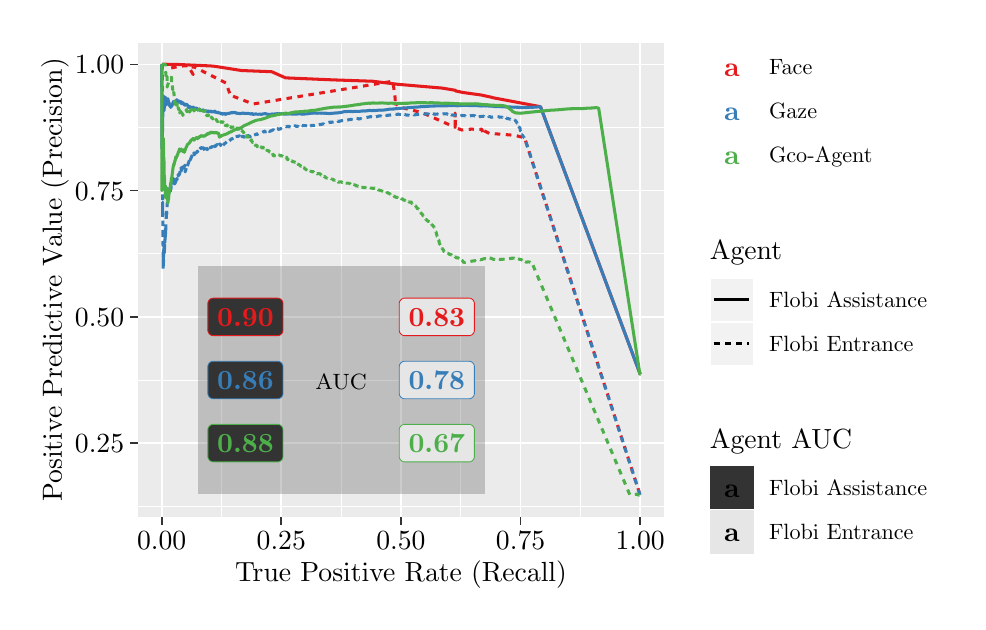
\begin{tikzpicture}[x=1pt,y=1pt]
\definecolor{fillColor}{RGB}{255,255,255}
\path[use as bounding box,fill=fillColor,fill opacity=0.00] (0,0) rectangle (336.00,207.65);
\begin{scope}
\path[clip] (  0.00,  0.00) rectangle (336.00,207.65);
\definecolor{drawColor}{RGB}{255,255,255}
\definecolor{fillColor}{RGB}{255,255,255}

\path[draw=drawColor,line width= 0.6pt,line join=round,line cap=round,fill=fillColor] (  0.00,  0.00) rectangle (336.00,207.65);
\end{scope}
\begin{scope}
\path[clip] ( 39.80, 30.86) rectangle (229.98,202.15);
\definecolor{fillColor}{gray}{0.92}

\path[fill=fillColor] ( 39.80, 30.86) rectangle (229.98,202.15);
\definecolor{drawColor}{RGB}{255,255,255}

\path[draw=drawColor,line width= 0.3pt,line join=round] ( 39.80, 34.72) --
	(229.98, 34.72);

\path[draw=drawColor,line width= 0.3pt,line join=round] ( 39.80, 80.33) --
	(229.98, 80.33);

\path[draw=drawColor,line width= 0.3pt,line join=round] ( 39.80,125.94) --
	(229.98,125.94);

\path[draw=drawColor,line width= 0.3pt,line join=round] ( 39.80,171.56) --
	(229.98,171.56);

\path[draw=drawColor,line width= 0.3pt,line join=round] ( 70.04, 30.86) --
	( 70.04,202.15);

\path[draw=drawColor,line width= 0.3pt,line join=round] (113.27, 30.86) --
	(113.27,202.15);

\path[draw=drawColor,line width= 0.3pt,line join=round] (156.49, 30.86) --
	(156.49,202.15);

\path[draw=drawColor,line width= 0.3pt,line join=round] (199.72, 30.86) --
	(199.72,202.15);

\path[draw=drawColor,line width= 0.6pt,line join=round] ( 39.80, 57.53) --
	(229.98, 57.53);

\path[draw=drawColor,line width= 0.6pt,line join=round] ( 39.80,103.14) --
	(229.98,103.14);

\path[draw=drawColor,line width= 0.6pt,line join=round] ( 39.80,148.75) --
	(229.98,148.75);

\path[draw=drawColor,line width= 0.6pt,line join=round] ( 39.80,194.36) --
	(229.98,194.36);

\path[draw=drawColor,line width= 0.6pt,line join=round] ( 48.42, 30.86) --
	( 48.42,202.15);

\path[draw=drawColor,line width= 0.6pt,line join=round] ( 91.65, 30.86) --
	( 91.65,202.15);

\path[draw=drawColor,line width= 0.6pt,line join=round] (134.88, 30.86) --
	(134.88,202.15);

\path[draw=drawColor,line width= 0.6pt,line join=round] (178.11, 30.86) --
	(178.11,202.15);

\path[draw=drawColor,line width= 0.6pt,line join=round] (221.34, 30.86) --
	(221.34,202.15);
\definecolor{fillColor}{RGB}{89,89,89}

\path[fill=fillColor,fill opacity=0.30] ( 61.39, 39.28) rectangle (165.14,121.38);
\definecolor{drawColor}{RGB}{0,0,0}

\node[text=drawColor,anchor=base,inner sep=0pt, outer sep=0pt, scale=  1.00] at (113.27, 76.87) {\footnotesize{AUC}};
\definecolor{drawColor}{RGB}{228,26,28}

\path[draw=drawColor,line width= 1.1pt,line join=round] ( 48.68,194.36) --
	( 52.40,194.36) --
	( 52.46,194.36) --
	( 54.16,194.36) --
	( 66.13,193.82) --
	( 66.14,193.82) --
	( 66.15,193.82) --
	( 67.56,193.69) --
	( 77.30,192.16) --
	( 88.14,191.73) --
	( 88.16,191.73) --
	( 88.17,191.73) --
	( 88.19,191.73) --
	( 93.19,189.51) --
	(110.19,188.79) --
	(124.15,188.31) --
	(124.52,188.30) --
	(124.65,188.29) --
	(133.69,187.19) --
	(149.76,185.82) --
	(154.46,185.03) --
	(154.54,184.96) --
	(154.72,184.77) --
	(157.33,184.22) --
	(163.87,183.32) --
	(167.96,182.42) --
	(168.19,182.32) --
	(185.31,179.09) --
	(221.34, 82.40);

\path[draw=drawColor,line width= 1.1pt,dash pattern=on 2pt off 2pt ,line join=round] ( 48.61,194.36) --
	( 48.98,194.36) --
	( 49.24,194.36) --
	( 50.63,194.36) --
	( 51.51,193.00) --
	( 55.08,193.73) --
	( 56.66,193.85) --
	( 57.85,193.91) --
	( 57.92,193.92) --
	( 57.94,193.92) --
	( 59.80,190.71) --
	( 59.80,193.62) --
	( 71.64,187.68) --
	( 73.38,182.91) --
	( 73.72,183.06) --
	( 81.48,180.07) --
	(131.87,188.28) --
	(132.27,186.07) --
	(132.80,182.01) --
	(132.85,179.40) --
	(132.85,180.42) --
	(134.24,179.00) --
	(142.46,176.96) --
	(154.48,171.64) --
	(154.48,176.24) --
	(154.48,176.69) --
	(154.48,176.79) --
	(154.51,171.34) --
	(155.41,171.24) --
	(156.85,170.67) --
	(160.08,170.90) --
	(160.08,171.04) --
	(161.82,170.87) --
	(164.16,170.95) --
	(164.37,169.64) --
	(164.37,170.08) --
	(164.37,170.68) --
	(166.79,169.46) --
	(176.09,168.75) --
	(179.62,167.78) --
	(179.67,167.50) --
	(221.34, 38.65);
\definecolor{drawColor}{RGB}{55,126,184}

\path[draw=drawColor,line width= 1.1pt,line join=round] ( 48.45,194.36) --
	( 48.47,163.95) --
	( 48.50,176.12) --
	( 48.52,166.29) --
	( 48.55,171.56) --
	( 48.57,175.16) --
	( 48.60,170.56) --
	( 48.63,173.31) --
	( 48.64,169.20) --
	( 48.66,165.85) --
	( 48.69,168.30) --
	( 48.74,172.11) --
	( 48.77,173.63) --
	( 48.80,175.36) --
	( 48.84,176.82) --
	( 48.86,177.78) --
	( 48.89,178.63) --
	( 48.92,179.41) --
	( 48.94,180.11) --
	( 48.97,180.75) --
	( 48.99,181.33) --
	( 49.02,181.87) --
	( 49.05,182.36) --
	( 49.08,182.96) --
	( 49.10,181.17) --
	( 49.13,181.63) --
	( 49.15,182.06) --
	( 49.19,182.59) --
	( 49.21,179.31) --
	( 49.23,179.77) --
	( 49.26,180.19) --
	( 49.28,178.87) --
	( 49.29,177.62) --
	( 49.33,178.22) --
	( 49.36,178.63) --
	( 49.38,179.03) --
	( 49.41,179.41) --
	( 49.44,179.77) --
	( 49.46,180.11) --
	( 49.50,180.54) --
	( 49.52,180.85) --
	( 49.55,181.14) --
	( 49.57,180.13) --
	( 49.60,180.52) --
	( 49.64,180.89) --
	( 49.67,181.24) --
	( 49.70,181.50) --
	( 49.73,181.74) --
	( 49.76,182.05) --
	( 49.79,182.27) --
	( 49.81,182.49) --
	( 49.83,181.63) --
	( 49.86,181.85) --
	( 49.89,182.13) --
	( 49.90,180.33) --
	( 49.94,180.63) --
	( 49.97,180.92) --
	( 50.00,180.26) --
	( 50.03,180.54) --
	( 50.06,179.91) --
	( 50.09,180.12) --
	( 50.11,180.33) --
	( 50.14,179.73) --
	( 50.17,179.94) --
	( 50.21,180.26) --
	( 50.24,180.45) --
	( 50.26,180.64) --
	( 50.30,180.88) --
	( 50.33,181.11) --
	( 50.36,181.28) --
	( 50.39,181.44) --
	( 50.40,180.85) --
	( 50.44,181.07) --
	( 50.47,181.23) --
	( 50.50,181.43) --
	( 50.54,181.63) --
	( 50.55,181.08) --
	( 50.60,181.33) --
	( 50.62,181.48) --
	( 50.65,181.62) --
	( 50.69,181.80) --
	( 50.72,181.98) --
	( 50.75,180.92) --
	( 50.77,181.06) --
	( 50.80,181.20) --
	( 50.83,181.33) --
	( 50.85,180.89) --
	( 50.87,180.42) --
	( 50.90,180.56) --
	( 50.92,180.69) --
	( 50.95,180.28) --
	( 50.98,180.42) --
	( 51.00,180.55) --
	( 51.02,180.11) --
	( 51.05,180.24) --
	( 51.07,180.37) --
	( 51.11,180.54) --
	( 51.13,180.66) --
	( 51.15,180.24) --
	( 51.18,179.87) --
	( 51.20,180.00) --
	( 51.23,180.12) --
	( 51.25,179.72) --
	( 51.27,179.33) --
	( 51.29,179.46) --
	( 51.32,179.58) --
	( 51.34,179.20) --
	( 51.37,179.37) --
	( 51.40,179.49) --
	( 51.42,179.61) --
	( 51.45,179.28) --
	( 51.48,179.40) --
	( 51.50,179.52) --
	( 51.53,179.20) --
	( 51.56,179.31) --
	( 51.57,178.96) --
	( 51.60,179.08) --
	( 51.63,179.20) --
	( 51.65,178.89) --
	( 51.68,179.01) --
	( 51.71,179.12) --
	( 51.73,178.83) --
	( 51.76,178.94) --
	( 51.79,179.05) --
	( 51.81,179.16) --
	( 51.84,179.27) --
	( 51.87,179.37) --
	( 51.89,179.09) --
	( 51.92,179.19) --
	( 51.95,179.33) --
	( 52.01,179.54) --
	( 52.04,179.67) --
	( 52.06,179.36) --
	( 52.09,179.49) --
	( 52.12,179.59) --
	( 52.16,179.72) --
	( 52.17,179.42) --
	( 52.20,179.52) --
	( 52.23,179.61) --
	( 52.25,179.70) --
	( 52.29,179.83) --
	( 52.31,179.92) --
	( 52.34,180.01) --
	( 52.38,180.13) --
	( 52.41,180.24) --
	( 52.44,180.33) --
	( 52.46,180.41) --
	( 52.50,180.52) --
	( 52.53,180.63) --
	( 52.56,180.71) --
	( 52.59,180.79) --
	( 52.61,180.87) --
	( 52.64,180.95) --
	( 52.67,181.03) --
	( 52.68,180.76) --
	( 52.71,180.83) --
	( 52.73,180.57) --
	( 52.75,180.64) --
	( 52.80,180.77) --
	( 52.82,180.51) --
	( 52.84,180.59) --
	( 52.87,180.66) --
	( 52.89,180.40) --
	( 52.92,180.51) --
	( 52.95,180.58) --
	( 52.98,180.68) --
	( 53.00,180.13) --
	( 53.03,180.20) --
	( 53.05,180.28) --
	( 53.08,180.35) --
	( 53.11,180.43) --
	( 53.14,180.52) --
	( 53.16,180.28) --
	( 53.19,180.35) --
	( 53.21,180.42) --
	( 53.24,180.49) --
	( 53.27,180.56) --
	( 53.29,180.63) --
	( 53.31,180.40) --
	( 53.34,180.47) --
	( 53.36,180.54) --
	( 53.39,180.60) --
	( 53.42,180.69) --
	( 53.46,180.78) --
	( 53.49,180.85) --
	( 53.51,180.91) --
	( 53.54,180.98) --
	( 53.56,181.04) --
	( 53.62,181.17) --
	( 53.64,181.23) --
	( 53.67,181.29) --
	( 53.70,181.35) --
	( 53.72,181.41) --
	( 53.75,181.47) --
	( 53.78,181.53) --
	( 53.81,181.61) --
	( 53.83,181.39) --
	( 53.86,181.45) --
	( 53.89,181.53) --
	( 53.92,181.58) --
	( 53.94,181.64) --
	( 53.96,181.43) --
	( 53.98,181.22) --
	( 54.00,181.01) --
	( 54.01,180.80) --
	( 54.03,180.59) --
	( 54.06,180.65) --
	( 54.08,180.71) --
	( 54.11,180.77) --
	( 54.13,180.57) --
	( 54.18,180.69) --
	( 54.22,180.76) --
	( 54.23,180.56) --
	( 54.26,180.62) --
	( 54.29,180.68) --
	( 54.31,180.74) --
	( 54.34,180.79) --
	( 54.37,180.85) --
	( 54.39,180.90) --
	( 54.42,180.96) --
	( 54.44,181.01) --
	( 54.47,181.07) --
	( 54.50,181.12) --
	( 54.52,181.17) --
	( 54.56,181.24) --
	( 54.58,181.05) --
	( 54.60,181.11) --
	( 54.62,180.92) --
	( 54.65,180.97) --
	( 54.67,181.02) --
	( 54.70,181.08) --
	( 54.73,181.13) --
	( 54.75,180.96) --
	( 54.78,181.01) --
	( 54.80,180.83) --
	( 54.83,180.90) --
	( 54.85,180.72) --
	( 54.88,180.77) --
	( 54.90,180.82) --
	( 54.93,180.87) --
	( 54.95,180.70) --
	( 54.97,180.75) --
	( 55.01,180.81) --
	( 55.03,180.66) --
	( 55.07,180.72) --
	( 55.10,180.77) --
	( 55.11,180.60) --
	( 55.14,180.65) --
	( 55.18,180.72) --
	( 55.21,180.78) --
	( 55.24,180.83) --
	( 55.26,180.88) --
	( 55.29,180.93) --
	( 55.32,180.98) --
	( 55.34,180.62) --
	( 55.36,180.46) --
	( 55.39,180.51) --
	( 55.40,180.34) --
	( 55.43,180.39) --
	( 55.46,180.25) --
	( 55.49,180.31) --
	( 55.52,180.36) --
	( 55.55,180.42) --
	( 55.59,180.49) --
	( 55.61,180.33) --
	( 55.63,180.38) --
	( 55.66,180.42) --
	( 55.69,180.47) --
	( 55.71,180.33) --
	( 55.74,180.37) --
	( 55.76,180.22) --
	( 55.80,180.30) --
	( 55.83,180.34) --
	( 55.86,180.40) --
	( 55.89,180.45) --
	( 55.92,180.50) --
	( 55.95,180.56) --
	( 55.99,180.61) --
	( 56.00,180.46) --
	( 56.04,180.52) --
	( 56.06,180.37) --
	( 56.07,180.22) --
	( 56.11,180.28) --
	( 56.14,180.33) --
	( 56.16,180.37) --
	( 56.20,180.43) --
	( 56.21,180.28) --
	( 56.24,180.33) --
	( 56.27,180.37) --
	( 56.29,180.41) --
	( 56.30,180.08) --
	( 56.33,180.13) --
	( 56.36,180.17) --
	( 56.37,180.03) --
	( 56.39,179.89) --
	( 56.42,179.93) --
	( 56.44,179.97) --
	( 56.47,180.02) --
	( 56.50,179.89) --
	( 56.53,179.95) --
	( 56.57,179.84) --
	( 56.59,179.88) --
	( 56.62,179.76) --
	( 56.65,179.80) --
	( 56.68,179.86) --
	( 56.71,179.90) --
	( 56.74,179.96) --
	( 56.77,180.00) --
	( 56.80,180.06) --
	( 56.82,179.92) --
	( 56.85,179.96) --
	( 56.87,179.83) --
	( 56.89,179.87) --
	( 56.91,179.74) --
	( 56.93,179.61) --
	( 56.95,179.65) --
	( 56.98,179.69) --
	( 57.01,179.73) --
	( 57.04,179.79) --
	( 57.06,179.66) --
	( 57.10,179.71) --
	( 57.13,179.77) --
	( 57.17,179.82) --
	( 57.19,179.86) --
	( 57.22,179.90) --
	( 57.24,179.94) --
	( 57.26,179.81) --
	( 57.29,179.85) --
	( 57.32,179.89) --
	( 57.35,179.95) --
	( 57.38,179.98) --
	( 57.40,179.72) --
	( 57.43,179.76) --
	( 57.46,179.81) --
	( 57.49,179.85) --
	( 57.51,179.73) --
	( 57.54,179.77) --
	( 57.56,179.81) --
	( 57.59,179.84) --
	( 57.62,179.89) --
	( 57.65,179.79) --
	( 57.68,179.68) --
	( 57.72,179.74) --
	( 57.74,179.62) --
	( 57.76,179.50) --
	( 57.78,179.54) --
	( 57.81,179.58) --
	( 57.84,179.63) --
	( 57.87,179.38) --
	( 57.91,179.43) --
	( 57.92,179.31) --
	( 57.95,179.35) --
	( 57.98,179.39) --
	( 57.98,179.12) --
	( 57.99,178.85) --
	( 58.02,178.89) --
	( 58.04,178.78) --
	( 58.07,178.83) --
	( 58.12,178.89) --
	( 58.14,178.79) --
	( 58.17,178.83) --
	( 58.20,178.87) --
	( 58.22,178.91) --
	( 58.24,178.80) --
	( 58.27,178.83) --
	( 58.30,178.89) --
	( 58.33,178.92) --
	( 58.36,178.97) --
	( 58.40,179.02) --
	( 58.42,179.06) --
	( 58.45,179.10) --
	( 58.49,179.15) --
	( 58.52,179.19) --
	( 58.55,179.10) --
	( 58.57,178.86) --
	( 58.59,178.89) --
	( 58.61,178.79) --
	( 58.64,178.82) --
	( 58.66,178.86) --
	( 58.68,178.75) --
	( 58.71,178.66) --
	( 58.73,178.70) --
	( 58.75,178.59) --
	( 58.78,178.63) --
	( 58.81,178.68) --
	( 58.83,178.57) --
	( 58.86,178.61) --
	( 58.89,178.66) --
	( 58.92,178.69) --
	( 58.94,178.59) --
	( 58.97,178.64) --
	( 59.00,178.67) --
	( 59.02,178.71) --
	( 59.05,178.74) --
	( 59.08,178.78) --
	( 59.10,178.81) --
	( 59.13,178.85) --
	( 59.16,178.88) --
	( 59.18,178.92) --
	( 59.20,178.82) --
	( 59.23,178.85) --
	( 59.25,178.89) --
	( 59.28,178.92) --
	( 59.30,178.82) --
	( 59.33,178.87) --
	( 59.35,178.77) --
	( 59.38,178.80) --
	( 59.40,178.83) --
	( 59.42,178.74) --
	( 59.45,178.65) --
	( 59.47,178.56) --
	( 59.53,178.64) --
	( 59.56,178.67) --
	( 59.60,178.72) --
	( 59.62,178.75) --
	( 59.65,178.79) --
	( 59.68,178.83) --
	( 59.71,178.75) --
	( 59.75,178.79) --
	( 59.77,178.82) --
	( 59.80,178.86) --
	( 59.82,178.89) --
	( 59.85,178.92) --
	( 59.88,178.95) --
	( 59.90,178.86) --
	( 59.92,178.77) --
	( 59.94,178.68) --
	( 59.97,178.71) --
	( 59.99,178.63) --
	( 60.01,178.54) --
	( 60.04,178.57) --
	( 60.05,178.36) --
	( 60.09,178.40) --
	( 60.12,178.44) --
	( 60.14,178.47) --
	( 60.16,178.38) --
	( 60.19,178.41) --
	( 60.20,178.32) --
	( 60.23,178.35) --
	( 60.26,178.38) --
	( 60.28,178.42) --
	( 60.32,178.46) --
	( 60.34,178.49) --
	( 60.38,178.53) --
	( 60.41,178.57) --
	( 60.42,178.48) --
	( 60.45,178.51) --
	( 60.47,178.42) --
	( 60.49,178.45) --
	( 60.52,178.48) --
	( 60.55,178.51) --
	( 60.57,178.54) --
	( 60.61,178.59) --
	( 60.63,178.51) --
	( 60.66,178.54) --
	( 60.69,178.57) --
	( 60.71,178.60) --
	( 60.75,178.64) --
	( 60.77,178.55) --
	( 60.78,178.47) --
	( 60.82,178.51) --
	( 60.85,178.54) --
	( 60.87,178.57) --
	( 60.89,178.48) --
	( 60.92,178.51) --
	( 60.93,178.20) --
	( 60.95,178.23) --
	( 60.98,178.26) --
	( 61.01,178.30) --
	( 61.04,178.34) --
	( 61.07,178.37) --
	( 61.09,178.40) --
	( 61.12,178.43) --
	( 61.15,178.46) --
	( 61.17,178.49) --
	( 61.22,178.43) --
	( 61.24,178.36) --
	( 61.27,178.39) --
	( 61.29,178.30) --
	( 61.31,178.23) --
	( 61.35,178.27) --
	( 61.37,178.19) --
	( 61.39,178.22) --
	( 61.42,178.25) --
	( 61.44,177.96) --
	( 61.45,177.88) --
	( 61.48,177.91) --
	( 61.52,177.95) --
	( 61.53,177.87) --
	( 61.57,177.91) --
	( 61.59,177.94) --
	( 61.62,177.97) --
	( 61.65,178.00) --
	( 61.67,178.03) --
	( 61.70,178.06) --
	( 61.74,178.10) --
	( 61.74,177.91) --
	( 61.78,177.95) --
	( 61.81,177.97) --
	( 61.83,178.00) --
	( 61.86,178.03) --
	( 61.88,178.06) --
	( 61.91,178.09) --
	( 61.94,178.12) --
	( 61.96,178.15) --
	( 62.00,178.19) --
	( 62.03,178.22) --
	( 62.05,178.24) --
	( 62.07,178.17) --
	( 62.10,178.19) --
	( 62.12,178.13) --
	( 62.14,178.05) --
	( 62.17,178.08) --
	( 62.19,178.10) --
	( 62.20,177.92) --
	( 62.23,177.95) --
	( 62.25,177.87) --
	( 62.27,177.90) --
	( 62.30,177.93) --
	( 62.34,177.98) --
	( 62.37,178.00) --
	( 62.39,177.93) --
	( 62.41,177.96) --
	( 62.43,177.88) --
	( 62.44,177.70) --
	( 62.47,177.73) --
	( 62.50,177.77) --
	( 62.53,177.79) --
	( 62.55,177.82) --
	( 62.57,177.75) --
	( 62.59,177.67) --
	( 62.62,177.70) --
	( 62.64,177.73) --
	( 62.67,177.76) --
	( 62.69,177.68) --
	( 62.71,177.71) --
	( 62.74,177.74) --
	( 62.77,177.77) --
	( 62.80,177.80) --
	( 62.83,177.83) --
	( 62.84,177.76) --
	( 62.87,177.79) --
	( 62.91,177.83) --
	( 62.92,177.66) --
	( 62.96,177.69) --
	( 62.99,177.73) --
	( 63.03,177.77) --
	( 63.06,177.79) --
	( 63.08,177.82) --
	( 63.12,177.86) --
	( 63.14,177.88) --
	( 63.17,177.91) --
	( 63.19,177.84) --
	( 63.21,177.87) --
	( 63.25,177.90) --
	( 63.28,177.93) --
	( 63.29,177.86) --
	( 63.32,177.88) --
	( 63.34,177.81) --
	( 63.36,177.84) --
	( 63.39,177.86) --
	( 63.42,177.89) --
	( 63.44,177.92) --
	( 63.46,177.85) --
	( 63.49,177.78) --
	( 63.52,177.82) --
	( 63.55,177.85) --
	( 63.57,177.78) --
	( 63.59,177.80) --
	( 63.60,177.64) --
	( 63.63,177.66) --
	( 63.65,177.69) --
	( 63.68,177.72) --
	( 63.70,177.65) --
	( 63.73,177.68) --
	( 63.76,177.71) --
	( 63.79,177.73) --
	( 63.80,177.66) --
	( 63.84,177.70) --
	( 63.87,177.72) --
	( 63.87,177.56) --
	( 63.90,177.59) --
	( 63.93,177.61) --
	( 63.95,177.64) --
	( 63.97,177.57) --
	( 63.99,177.50) --
	( 64.03,177.55) --
	( 64.06,177.57) --
	( 64.09,177.60) --
	( 64.10,177.53) --
	( 64.13,177.56) --
	( 64.17,177.59) --
	( 64.20,177.62) --
	( 64.24,177.66) --
	( 64.24,177.42) --
	( 64.27,177.44) --
	( 64.30,177.47) --
	( 64.33,177.50) --
	( 64.36,177.53) --
	( 64.39,177.55) --
	( 64.41,177.58) --
	( 64.45,177.61) --
	( 64.46,177.46) --
	( 64.49,177.49) --
	( 64.52,177.51) --
	( 64.54,177.54) --
	( 64.56,177.47) --
	( 64.59,177.50) --
	( 64.62,177.53) --
	( 64.66,177.56) --
	( 64.68,177.50) --
	( 64.71,177.53) --
	( 64.74,177.56) --
	( 64.76,177.50) --
	( 64.79,177.52) --
	( 64.82,177.55) --
	( 64.83,177.49) --
	( 64.85,177.42) --
	( 64.89,177.45) --
	( 64.91,177.40) --
	( 64.95,177.43) --
	( 64.97,177.37) --
	( 64.98,177.30) --
	( 65.01,177.33) --
	( 65.04,177.35) --
	( 65.06,177.38) --
	( 65.10,177.41) --
	( 65.12,177.35) --
	( 65.15,177.38) --
	( 65.18,177.40) --
	( 65.21,177.44) --
	( 65.24,177.46) --
	( 65.27,177.48) --
	( 65.30,177.52) --
	( 65.33,177.54) --
	( 65.35,177.56) --
	( 65.38,177.59) --
	( 65.39,177.44) --
	( 65.42,177.47) --
	( 65.44,177.41) --
	( 65.45,177.26) --
	( 65.48,177.29) --
	( 65.51,177.32) --
	( 65.54,177.34) --
	( 65.57,177.37) --
	( 65.59,177.39) --
	( 65.61,177.33) --
	( 65.65,177.37) --
	( 65.67,177.31) --
	( 65.69,177.25) --
	( 65.71,177.27) --
	( 65.74,177.29) --
	( 65.78,177.25) --
	( 65.80,177.27) --
	( 65.84,177.30) --
	( 65.86,177.33) --
	( 65.89,177.35) --
	( 65.93,177.38) --
	( 65.94,177.32) --
	( 65.97,177.35) --
	( 66.00,177.37) --
	( 66.03,177.40) --
	( 66.06,177.42) --
	( 66.08,177.45) --
	( 66.11,177.47) --
	( 66.14,177.49) --
	( 66.16,177.51) --
	( 66.19,177.54) --
	( 66.20,177.40) --
	( 66.23,177.34) --
	( 66.25,177.37) --
	( 66.27,177.31) --
	( 66.29,177.25) --
	( 66.31,177.27) --
	( 66.34,177.22) --
	( 66.37,177.24) --
	( 66.39,177.27) --
	( 66.42,177.29) --
	( 66.44,177.23) --
	( 66.45,177.17) --
	( 66.48,177.20) --
	( 66.51,177.22) --
	( 66.52,177.16) --
	( 66.55,177.18) --
	( 66.58,177.21) --
	( 66.61,177.24) --
	( 66.64,177.26) --
	( 66.67,177.21) --
	( 66.69,177.23) --
	( 66.72,177.26) --
	( 66.74,177.20) --
	( 66.77,177.23) --
	( 66.79,177.17) --
	( 66.82,177.19) --
	( 66.84,177.22) --
	( 66.87,177.24) --
	( 66.90,177.27) --
	( 66.94,177.30) --
	( 66.97,177.32) --
	( 66.99,177.34) --
	( 67.02,177.36) --
	( 67.04,177.31) --
	( 67.06,177.33) --
	( 67.09,177.35) --
	( 67.11,177.37) --
	( 67.15,177.40) --
	( 67.17,177.27) --
	( 67.19,177.22) --
	( 67.22,177.25) --
	( 67.25,177.27) --
	( 67.27,177.29) --
	( 67.30,177.31) --
	( 67.35,177.36) --
	( 67.38,177.31) --
	( 67.41,177.33) --
	( 67.43,177.35) --
	( 67.46,177.37) --
	( 67.48,177.39) --
	( 67.51,177.42) --
	( 67.56,177.45) --
	( 67.59,177.48) --
	( 67.62,177.50) --
	( 67.65,177.53) --
	( 67.67,177.47) --
	( 67.67,177.20) --
	( 67.70,177.22) --
	( 67.72,177.24) --
	( 67.75,177.26) --
	( 67.77,177.21) --
	( 67.79,177.23) --
	( 67.81,177.18) --
	( 67.84,177.06) --
	( 67.86,177.08) --
	( 67.90,177.11) --
	( 67.94,177.15) --
	( 67.96,177.09) --
	( 68.00,177.12) --
	( 68.02,177.14) --
	( 68.05,177.16) --
	( 68.07,177.11) --
	( 68.10,177.14) --
	( 68.13,177.09) --
	( 68.15,177.11) --
	( 68.18,177.07) --
	( 68.21,177.09) --
	( 68.22,177.04) --
	( 68.25,177.06) --
	( 68.27,177.00) --
	( 68.30,177.03) --
	( 68.32,176.98) --
	( 68.36,177.01) --
	( 68.38,177.03) --
	( 68.40,176.98) --
	( 68.44,177.01) --
	( 68.47,177.03) --
	( 68.50,177.05) --
	( 68.52,177.07) --
	( 68.54,177.02) --
	( 68.57,177.04) --
	( 68.59,176.99) --
	( 68.61,177.01) --
	( 68.64,177.03) --
	( 68.66,177.05) --
	( 68.71,177.09) --
	( 68.74,177.11) --
	( 68.76,177.06) --
	( 68.77,176.94) --
	( 68.80,176.96) --
	( 68.82,176.98) --
	( 68.87,177.01) --
	( 68.89,177.03) --
	( 68.91,176.98) --
	( 68.94,177.00) --
	( 68.95,176.95) --
	( 68.98,176.84) --
	( 69.02,176.87) --
	( 69.04,176.89) --
	( 69.07,176.91) --
	( 69.10,176.93) --
	( 69.12,176.95) --
	( 69.16,176.98) --
	( 69.19,177.01) --
	( 69.23,177.03) --
	( 69.25,176.99) --
	( 69.27,176.94) --
	( 69.30,176.90) --
	( 69.32,176.85) --
	( 69.34,176.87) --
	( 69.37,176.82) --
	( 69.40,176.84) --
	( 69.41,176.80) --
	( 69.45,176.82) --
	( 69.47,176.84) --
	( 69.50,176.86) --
	( 69.53,176.82) --
	( 69.55,176.78) --
	( 69.58,176.80) --
	( 69.59,176.68) --
	( 69.62,176.70) --
	( 69.66,176.73) --
	( 69.69,176.75) --
	( 69.71,176.77) --
	( 69.75,176.80) --
	( 69.76,176.62) --
	( 69.77,176.57) --
	( 69.82,176.61) --
	( 69.84,176.63) --
	( 69.87,176.58) --
	( 69.92,176.62) --
	( 69.94,176.58) --
	( 69.96,176.53) --
	( 69.99,176.55) --
	( 70.00,176.50) --
	( 70.03,176.52) --
	( 70.06,176.54) --
	( 70.08,176.56) --
	( 70.10,176.51) --
	( 70.13,176.53) --
	( 70.15,176.55) --
	( 70.19,176.58) --
	( 70.22,176.60) --
	( 70.25,176.62) --
	( 70.27,176.52) --
	( 70.28,176.41) --
	( 70.32,176.43) --
	( 70.34,176.39) --
	( 70.36,176.41) --
	( 70.40,176.43) --
	( 70.43,176.45) --
	( 70.46,176.48) --
	( 70.48,176.43) --
	( 70.50,176.39) --
	( 70.53,176.41) --
	( 70.56,176.43) --
	( 70.59,176.46) --
	( 70.63,176.48) --
	( 70.65,176.50) --
	( 70.68,176.52) --
	( 70.71,176.54) --
	( 70.74,176.57) --
	( 70.77,176.58) --
	( 70.80,176.61) --
	( 70.84,176.58) --
	( 70.87,176.60) --
	( 70.88,176.55) --
	( 70.91,176.57) --
	( 70.94,176.59) --
	( 70.96,176.55) --
	( 70.98,176.50) --
	( 71.03,176.54) --
	( 71.06,176.56) --
	( 71.09,176.58) --
	( 71.13,176.61) --
	( 71.14,176.50) --
	( 71.16,176.52) --
	( 71.19,176.54) --
	( 71.23,176.56) --
	( 71.25,176.58) --
	( 71.28,176.60) --
	( 71.29,176.49) --
	( 71.32,176.52) --
	( 71.36,176.54) --
	( 71.39,176.56) --
	( 71.40,176.51) --
	( 71.42,176.47) --
	( 71.44,176.43) --
	( 71.46,176.32) --
	( 71.48,176.34) --
	( 71.51,176.36) --
	( 71.53,176.32) --
	( 71.56,176.34) --
	( 71.59,176.36) --
	( 71.61,176.32) --
	( 71.65,176.35) --
	( 71.68,176.37) --
	( 71.70,176.38) --
	( 71.73,176.40) --
	( 71.75,176.42) --
	( 71.79,176.45) --
	( 71.83,176.47) --
	( 71.85,176.49) --
	( 71.89,176.51) --
	( 71.91,176.53) --
	( 71.94,176.55) --
	( 71.96,176.45) --
	( 71.98,176.47) --
	( 72.02,176.49) --
	( 72.05,176.51) --
	( 72.07,176.53) --
	( 72.10,176.55) --
	( 72.12,176.56) --
	( 72.15,176.58) --
	( 72.19,176.61) --
	( 72.22,176.63) --
	( 72.26,176.65) --
	( 72.28,176.67) --
	( 72.32,176.69) --
	( 72.34,176.71) --
	( 72.36,176.67) --
	( 72.40,176.69) --
	( 72.44,176.72) --
	( 72.47,176.74) --
	( 72.49,176.70) --
	( 72.51,176.71) --
	( 72.54,176.68) --
	( 72.56,176.69) --
	( 72.59,176.71) --
	( 72.62,176.67) --
	( 72.64,176.69) --
	( 72.68,176.72) --
	( 72.71,176.73) --
	( 72.72,176.69) --
	( 72.75,176.71) --
	( 72.77,176.67) --
	( 72.79,176.68) --
	( 72.82,176.70) --
	( 72.84,176.66) --
	( 72.87,176.68) --
	( 72.90,176.64) --
	( 72.93,176.66) --
	( 72.95,176.68) --
	( 72.99,176.70) --
	( 73.02,176.72) --
	( 73.05,176.74) --
	( 73.08,176.76) --
	( 73.12,176.79) --
	( 73.15,176.81) --
	( 73.18,176.83) --
	( 73.21,176.84) --
	( 73.23,176.86) --
	( 73.26,176.88) --
	( 73.28,176.84) --
	( 73.30,176.85) --
	( 73.32,176.81) --
	( 73.36,176.83) --
	( 73.38,176.85) --
	( 73.42,176.87) --
	( 73.45,176.89) --
	( 73.48,176.91) --
	( 73.52,176.93) --
	( 73.56,176.96) --
	( 73.59,176.98) --
	( 73.61,176.99) --
	( 73.63,176.90) --
	( 73.67,176.92) --
	( 73.69,176.94) --
	( 73.71,176.85) --
	( 73.74,176.86) --
	( 73.76,176.83) --
	( 73.79,176.84) --
	( 73.82,176.87) --
	( 73.85,176.88) --
	( 73.88,176.90) --
	( 73.90,176.92) --
	( 73.94,176.94) --
	( 73.96,176.95) --
	( 73.99,176.97) --
	( 74.03,176.99) --
	( 74.04,176.95) --
	( 74.05,176.85) --
	( 74.10,176.88) --
	( 74.12,176.90) --
	( 74.16,176.92) --
	( 74.19,176.94) --
	( 74.23,176.96) --
	( 74.26,176.98) --
	( 74.28,176.99) --
	( 74.31,177.01) --
	( 74.33,177.03) --
	( 74.36,177.04) --
	( 74.39,177.06) --
	( 74.41,177.02) --
	( 74.44,177.04) --
	( 74.47,177.00) --
	( 74.49,177.02) --
	( 74.52,176.99) --
	( 74.54,176.95) --
	( 74.56,176.96) --
	( 74.59,176.98) --
	( 74.62,176.99) --
	( 74.64,177.01) --
	( 74.67,176.98) --
	( 74.70,176.94) --
	( 74.72,176.96) --
	( 74.76,176.98) --
	( 74.77,176.94) --
	( 74.79,176.90) --
	( 74.83,176.92) --
	( 74.85,176.94) --
	( 74.87,176.90) --
	( 74.90,176.91) --
	( 74.92,176.93) --
	( 74.95,176.94) --
	( 74.98,176.96) --
	( 74.99,176.92) --
	( 75.02,176.94) --
	( 75.04,176.85) --
	( 75.07,176.86) --
	( 75.08,176.83) --
	( 75.11,176.84) --
	( 75.14,176.81) --
	( 75.16,176.82) --
	( 75.19,176.84) --
	( 75.22,176.81) --
	( 75.24,176.77) --
	( 75.27,176.79) --
	( 75.30,176.81) --
	( 75.36,176.84) --
	( 75.39,176.86) --
	( 75.41,176.82) --
	( 75.44,176.84) --
	( 75.46,176.85) --
	( 75.47,176.76) --
	( 75.49,176.72) --
	( 75.51,176.74) --
	( 75.54,176.75) --
	( 75.57,176.72) --
	( 75.59,176.74) --
	( 75.63,176.76) --
	( 75.65,176.72) --
	( 75.67,176.74) --
	( 75.70,176.75) --
	( 75.73,176.77) --
	( 75.74,176.73) --
	( 75.76,176.69) --
	( 75.79,176.71) --
	( 75.81,176.72) --
	( 75.84,176.69) --
	( 75.88,176.71) --
	( 75.92,176.69) --
	( 75.95,176.70) --
	( 75.96,176.67) --
	( 75.99,176.68) --
	( 76.00,176.59) --
	( 76.03,176.61) --
	( 76.07,176.63) --
	( 76.10,176.60) --
	( 76.12,176.61) --
	( 76.16,176.64) --
	( 76.19,176.61) --
	( 76.21,176.57) --
	( 76.25,176.59) --
	( 76.27,176.61) --
	( 76.31,176.63) --
	( 76.34,176.65) --
	( 76.37,176.66) --
	( 76.39,176.68) --
	( 76.41,176.64) --
	( 76.45,176.66) --
	( 76.47,176.68) --
	( 76.49,176.59) --
	( 76.51,176.56) --
	( 76.54,176.58) --
	( 76.57,176.59) --
	( 76.60,176.61) --
	( 76.62,176.62) --
	( 76.65,176.64) --
	( 76.67,176.55) --
	( 76.69,176.57) --
	( 76.71,176.53) --
	( 76.75,176.55) --
	( 76.78,176.57) --
	( 76.82,176.59) --
	( 76.84,176.56) --
	( 76.86,176.57) --
	( 76.89,176.59) --
	( 76.93,176.61) --
	( 76.96,176.63) --
	( 76.98,176.59) --
	( 77.01,176.61) --
	( 77.04,176.62) --
	( 77.06,176.64) --
	( 77.09,176.65) --
	( 77.13,176.68) --
	( 77.15,176.64) --
	( 77.18,176.66) --
	( 77.20,176.67) --
	( 77.23,176.69) --
	( 77.25,176.65) --
	( 77.28,176.67) --
	( 77.30,176.68) --
	( 77.34,176.70) --
	( 77.37,176.72) --
	( 77.41,176.74) --
	( 77.43,176.75) --
	( 77.46,176.77) --
	( 77.49,176.78) --
	( 77.52,176.80) --
	( 77.55,176.82) --
	( 77.57,176.78) --
	( 77.60,176.80) --
	( 77.63,176.81) --
	( 77.66,176.83) --
	( 77.67,176.75) --
	( 77.70,176.72) --
	( 77.73,176.74) --
	( 77.76,176.75) --
	( 77.79,176.77) --
	( 77.81,176.69) --
	( 77.84,176.70) --
	( 77.87,176.72) --
	( 77.89,176.69) --
	( 77.92,176.70) --
	( 77.94,176.67) --
	( 77.96,176.68) --
	( 77.99,176.70) --
	( 78.02,176.72) --
	( 78.04,176.68) --
	( 78.07,176.69) --
	( 78.09,176.71) --
	( 78.14,176.73) --
	( 78.16,176.75) --
	( 78.18,176.71) --
	( 78.20,176.68) --
	( 78.24,176.70) --
	( 78.28,176.72) --
	( 78.30,176.69) --
	( 78.31,176.61) --
	( 78.35,176.63) --
	( 78.38,176.64) --
	( 78.41,176.66) --
	( 78.44,176.63) --
	( 78.46,176.60) --
	( 78.49,176.61) --
	( 78.52,176.63) --
	( 78.54,176.64) --
	( 78.57,176.66) --
	( 78.62,176.68) --
	( 78.66,176.70) --
	( 78.68,176.72) --
	( 78.72,176.74) --
	( 78.74,176.70) --
	( 78.76,176.72) --
	( 78.78,176.68) --
	( 78.80,176.65) --
	( 78.83,176.67) --
	( 78.87,176.68) --
	( 78.90,176.70) --
	( 78.91,176.66) --
	( 78.95,176.68) --
	( 78.97,176.70) --
	( 79.02,176.72) --
	( 79.05,176.73) --
	( 79.08,176.75) --
	( 79.10,176.72) --
	( 79.12,176.68) --
	( 79.14,176.70) --
	( 79.16,176.66) --
	( 79.18,176.63) --
	( 79.20,176.65) --
	( 79.22,176.61) --
	( 79.25,176.63) --
	( 79.27,176.64) --
	( 79.30,176.65) --
	( 79.33,176.67) --
	( 79.34,176.63) --
	( 79.38,176.65) --
	( 79.41,176.67) --
	( 79.43,176.68) --
	( 79.47,176.70) --
	( 79.51,176.72) --
	( 79.54,176.69) --
	( 79.56,176.70) --
	( 79.60,176.72) --
	( 79.63,176.74) --
	( 79.65,176.67) --
	( 79.67,176.59) --
	( 79.71,176.61) --
	( 79.74,176.63) --
	( 79.78,176.64) --
	( 79.79,176.61) --
	( 79.83,176.63) --
	( 79.86,176.64) --
	( 79.88,176.66) --
	( 79.91,176.67) --
	( 79.93,176.64) --
	( 79.95,176.65) --
	( 79.98,176.66) --
	( 80.00,176.63) --
	( 80.01,176.60) --
	( 80.03,176.57) --
	( 80.07,176.58) --
	( 80.09,176.60) --
	( 80.12,176.57) --
	( 80.15,176.58) --
	( 80.17,176.60) --
	( 80.19,176.56) --
	( 80.22,176.54) --
	( 80.25,176.55) --
	( 80.27,176.52) --
	( 80.30,176.54) --
	( 80.33,176.55) --
	( 80.36,176.57) --
	( 80.38,176.58) --
	( 80.40,176.55) --
	( 80.42,176.52) --
	( 80.44,176.53) --
	( 80.45,176.45) --
	( 80.48,176.47) --
	( 80.51,176.48) --
	( 80.52,176.45) --
	( 80.54,176.41) --
	( 80.57,176.43) --
	( 80.59,176.44) --
	( 80.64,176.46) --
	( 80.68,176.49) --
	( 80.71,176.50) --
	( 80.74,176.51) --
	( 80.76,176.53) --
	( 80.79,176.54) --
	( 80.81,176.51) --
	( 80.84,176.52) --
	( 80.87,176.54) --
	( 80.89,176.55) --
	( 80.92,176.56) --
	( 80.96,176.58) --
	( 81.02,176.61) --
	( 81.04,176.62) --
	( 81.08,176.64) --
	( 81.10,176.57) --
	( 81.12,176.58) --
	( 81.14,176.51) --
	( 81.17,176.52) --
	( 81.20,176.54) --
	( 81.21,176.47) --
	( 81.24,176.48) --
	( 81.26,176.49) --
	( 81.28,176.34) --
	( 81.31,176.36) --
	( 81.33,176.37) --
	( 81.36,176.38) --
	( 81.39,176.39) --
	( 81.41,176.41) --
	( 81.42,176.33) --
	( 81.45,176.35) --
	( 81.47,176.31) --
	( 81.48,176.28) --
	( 81.52,176.30) --
	( 81.55,176.32) --
	( 81.58,176.33) --
	( 81.61,176.34) --
	( 81.64,176.36) --
	( 81.68,176.38) --
	( 81.70,176.35) --
	( 81.73,176.37) --
	( 81.76,176.38) --
	( 81.78,176.39) --
	( 81.81,176.40) --
	( 81.84,176.42) --
	( 81.86,176.43) --
	( 81.90,176.45) --
	( 81.92,176.46) --
	( 81.95,176.47) --
	( 81.98,176.48) --
	( 82.01,176.50) --
	( 82.03,176.47) --
	( 82.05,176.44) --
	( 82.07,176.45) --
	( 82.10,176.47) --
	( 82.12,176.40) --
	( 82.14,176.41) --
	( 82.17,176.42) --
	( 82.21,176.44) --
	( 82.23,176.45) --
	( 82.26,176.46) --
	( 82.28,176.43) --
	( 82.30,176.45) --
	( 82.33,176.46) --
	( 82.36,176.48) --
	( 82.39,176.49) --
	( 82.42,176.50) --
	( 82.45,176.52) --
	( 82.47,176.41) --
	( 82.51,176.43) --
	( 82.52,176.40) --
	( 82.55,176.41) --
	( 82.56,176.34) --
	( 82.58,176.35) --
	( 82.62,176.37) --
	( 82.65,176.38) --
	( 82.66,176.35) --
	( 82.70,176.37) --
	( 82.73,176.34) --
	( 82.75,176.35) --
	( 82.79,176.33) --
	( 82.81,176.34) --
	( 82.84,176.36) --
	( 82.86,176.33) --
	( 82.88,176.34) --
	( 82.91,176.35) --
	( 82.94,176.36) --
	( 82.96,176.38) --
	( 82.99,176.39) --
	( 83.01,176.36) --
	( 83.03,176.33) --
	( 83.05,176.31) --
	( 83.08,176.32) --
	( 83.10,176.29) --
	( 83.13,176.30) --
	( 83.16,176.32) --
	( 83.19,176.33) --
	( 83.22,176.35) --
	( 83.24,176.36) --
	( 83.27,176.37) --
	( 83.31,176.39) --
	( 83.32,176.36) --
	( 83.34,176.33) --
	( 83.38,176.35) --
	( 83.40,176.36) --
	( 83.43,176.37) --
	( 83.46,176.38) --
	( 83.48,176.39) --
	( 83.51,176.41) --
	( 83.54,176.38) --
	( 83.56,176.39) --
	( 83.59,176.41) --
	( 83.62,176.42) --
	( 83.67,176.44) --
	( 83.71,176.46) --
	( 83.74,176.47) --
	( 83.75,176.37) --
	( 83.77,176.38) --
	( 83.80,176.39) --
	( 83.83,176.41) --
	( 83.86,176.42) --
	( 83.89,176.43) --
	( 83.92,176.45) --
	( 83.94,176.42) --
	( 83.98,176.44) --
	( 83.99,176.41) --
	( 84.03,176.42) --
	( 84.06,176.44) --
	( 84.09,176.41) --
	( 84.11,176.39) --
	( 84.13,176.36) --
	( 84.15,176.37) --
	( 84.18,176.38) --
	( 84.20,176.39) --
	( 84.23,176.33) --
	( 84.26,176.34) --
	( 84.28,176.28) --
	( 84.29,176.25) --
	( 84.33,176.27) --
	( 84.35,176.28) --
	( 84.38,176.29) --
	( 84.42,176.31) --
	( 84.44,176.28) --
	( 84.47,176.29) --
	( 84.50,176.31) --
	( 84.52,176.32) --
	( 84.55,176.33) --
	( 84.57,176.34) --
	( 84.61,176.36) --
	( 84.64,176.37) --
	( 84.67,176.38) --
	( 84.71,176.40) --
	( 84.74,176.42) --
	( 84.77,176.43) --
	( 84.79,176.40) --
	( 84.81,176.41) --
	( 84.85,176.43) --
	( 84.87,176.44) --
	( 84.90,176.45) --
	( 84.94,176.47) --
	( 84.95,176.44) --
	( 84.99,176.45) --
	( 85.01,176.47) --
	( 85.04,176.48) --
	( 85.07,176.49) --
	( 85.10,176.50) --
	( 85.13,176.52) --
	( 85.15,176.49) --
	( 85.18,176.50) --
	( 85.20,176.48) --
	( 85.23,176.49) --
	( 85.26,176.50) --
	( 85.29,176.51) --
	( 85.31,176.49) --
	( 85.34,176.50) --
	( 85.37,176.51) --
	( 85.39,176.53) --
	( 85.42,176.54) --
	( 85.45,176.55) --
	( 85.48,176.56) --
	( 85.51,176.57) --
	( 85.53,176.59) --
	( 85.56,176.60) --
	( 85.58,176.57) --
	( 85.60,176.58) --
	( 85.62,176.55) --
	( 85.65,176.57) --
	( 85.67,176.58) --
	( 85.70,176.59) --
	( 85.73,176.60) --
	( 85.76,176.61) --
	( 85.79,176.63) --
	( 85.81,176.60) --
	( 85.83,176.61) --
	( 85.86,176.62) --
	( 85.89,176.63) --
	( 85.91,176.64) --
	( 85.95,176.66) --
	( 85.97,176.63) --
	( 86.00,176.65) --
	( 86.01,176.55) --
	( 86.02,176.48) --
	( 86.04,176.49) --
	( 86.07,176.50) --
	( 86.09,176.48) --
	( 86.12,176.49) --
	( 86.13,176.42) --
	( 86.15,176.40) --
	( 86.18,176.41) --
	( 86.20,176.42) --
	( 86.24,176.44) --
	( 86.26,176.45) --
	( 86.29,176.46) --
	( 86.32,176.47) --
	( 86.35,176.48) --
	( 86.38,176.50) --
	( 86.40,176.47) --
	( 86.41,176.44) --
	( 86.44,176.42) --
	( 86.48,176.43) --
	( 86.50,176.44) --
	( 86.53,176.46) --
	( 86.57,176.44) --
	( 86.60,176.45) --
	( 86.63,176.46) --
	( 86.64,176.40) --
	( 86.66,176.34) --
	( 86.69,176.35) --
	( 86.71,176.36) --
	( 86.72,176.30) --
	( 86.75,176.31) --
	( 86.77,176.28) --
	( 86.79,176.29) --
	( 86.82,176.31) --
	( 86.85,176.32) --
	( 86.88,176.33) --
	( 86.91,176.34) --
	( 86.93,176.35) --
	( 86.96,176.37) --
	( 86.99,176.38) --
	( 87.00,176.35) --
	( 87.03,176.33) --
	( 87.05,176.30) --
	( 87.08,176.32) --
	( 87.12,176.33) --
	( 87.15,176.35) --
	( 87.17,176.32) --
	( 87.20,176.33) --
	( 87.22,176.30) --
	( 87.25,176.32) --
	( 87.28,176.33) --
	( 87.30,176.34) --
	( 87.32,176.31) --
	( 87.35,176.29) --
	( 87.37,176.30) --
	( 87.40,176.28) --
	( 87.42,176.25) --
	( 87.44,176.27) --
	( 87.47,176.28) --
	( 87.50,176.25) --
	( 87.53,176.27) --
	( 87.56,176.28) --
	( 87.60,176.30) --
	( 87.63,176.31) --
	( 87.66,176.32) --
	( 87.68,176.33) --
	( 87.71,176.34) --
	( 87.74,176.32) --
	( 87.76,176.30) --
	( 87.79,176.31) --
	( 87.81,176.32) --
	( 87.84,176.33) --
	( 87.88,176.34) --
	( 87.90,176.36) --
	( 87.94,176.37) --
	( 87.96,176.38) --
	( 87.99,176.39) --
	( 88.02,176.40) --
	( 88.03,176.38) --
	( 88.06,176.39) --
	( 88.09,176.40) --
	( 88.11,176.37) --
	( 88.13,176.38) --
	( 88.16,176.39) --
	( 88.20,176.41) --
	( 88.24,176.43) --
	( 88.26,176.44) --
	( 88.29,176.45) --
	( 88.32,176.46) --
	( 88.35,176.47) --
	( 88.37,176.45) --
	( 88.40,176.46) --
	( 88.42,176.47) --
	( 88.45,176.48) --
	( 88.48,176.49) --
	( 88.51,176.50) --
	( 88.53,176.48) --
	( 88.55,176.45) --
	( 88.57,176.43) --
	( 88.59,176.41) --
	( 88.62,176.42) --
	( 88.65,176.43) --
	( 88.69,176.44) --
	( 88.70,176.42) --
	( 88.74,176.43) --
	( 88.77,176.44) --
	( 88.79,176.45) --
	( 88.82,176.47) --
	( 88.84,176.44) --
	( 88.86,176.45) --
	( 88.89,176.46) --
	( 88.92,176.44) --
	( 88.96,176.46) --
	( 88.98,176.43) --
	( 89.01,176.45) --
	( 89.04,176.46) --
	( 89.06,176.43) --
	( 89.09,176.45) --
	( 89.13,176.46) --
	( 89.15,176.47) --
	( 89.18,176.48) --
	( 89.21,176.49) --
	( 89.23,176.50) --
	( 89.26,176.51) --
	( 89.28,176.49) --
	( 89.30,176.43) --
	( 89.33,176.44) --
	( 89.36,176.46) --
	( 89.39,176.47) --
	( 89.42,176.48) --
	( 89.44,176.49) --
	( 89.47,176.47) --
	( 89.50,176.48) --
	( 89.52,176.46) --
	( 89.55,176.47) --
	( 89.58,176.48) --
	( 89.61,176.49) --
	( 89.64,176.50) --
	( 89.65,176.48) --
	( 89.68,176.49) --
	( 89.71,176.50) --
	( 89.73,176.47) --
	( 89.74,176.45) --
	( 89.77,176.46) --
	( 89.80,176.47) --
	( 89.83,176.48) --
	( 89.86,176.49) --
	( 89.88,176.50) --
	( 89.91,176.51) --
	( 89.95,176.53) --
	( 89.97,176.54) --
	( 90.01,176.55) --
	( 90.04,176.56) --
	( 90.07,176.57) --
	( 90.09,176.58) --
	( 90.13,176.57) --
	( 90.16,176.58) --
	( 90.19,176.59) --
	( 90.22,176.60) --
	( 90.24,176.58) --
	( 90.27,176.59) --
	( 90.29,176.56) --
	( 90.32,176.58) --
	( 90.35,176.59) --
	( 90.38,176.60) --
	( 90.41,176.61) --
	( 90.43,176.59) --
	( 90.46,176.60) --
	( 90.46,176.51) --
	( 90.49,176.52) --
	( 90.52,176.53) --
	( 90.54,176.54) --
	( 90.58,176.55) --
	( 90.59,176.49) --
	( 90.61,176.47) --
	( 90.63,176.48) --
	( 90.67,176.49) --
	( 90.71,176.51) --
	( 90.75,176.52) --
	( 90.77,176.53) --
	( 90.80,176.54) --
	( 90.83,176.55) --
	( 90.86,176.53) --
	( 90.90,176.55) --
	( 90.94,176.56) --
	( 90.98,176.58) --
	( 91.00,176.59) --
	( 91.03,176.60) --
	( 91.05,176.61) --
	( 91.09,176.59) --
	( 91.13,176.60) --
	( 91.13,176.54) --
	( 91.16,176.55) --
	( 91.18,176.53) --
	( 91.20,176.54) --
	( 91.23,176.55) --
	( 91.25,176.53) --
	( 91.27,176.54) --
	( 91.30,176.55) --
	( 91.34,176.53) --
	( 91.36,176.54) --
	( 91.40,176.55) --
	( 91.42,176.53) --
	( 91.44,176.54) --
	( 91.48,176.55) --
	( 91.50,176.56) --
	( 91.53,176.54) --
	( 91.55,176.52) --
	( 91.58,176.53) --
	( 91.62,176.54) --
	( 91.64,176.52) --
	( 91.65,176.50) --
	( 91.69,176.51) --
	( 91.71,176.52) --
	( 91.74,176.53) --
	( 91.77,176.54) --
	( 91.79,176.55) --
	( 91.82,176.56) --
	( 91.86,176.57) --
	( 91.88,176.58) --
	( 91.92,176.59) --
	( 91.94,176.57) --
	( 91.98,176.59) --
	( 92.01,176.60) --
	( 92.03,176.61) --
	( 92.05,176.58) --
	( 92.06,176.53) --
	( 92.08,176.54) --
	( 92.10,176.51) --
	( 92.14,176.53) --
	( 92.16,176.53) --
	( 92.19,176.54) --
	( 92.21,176.52) --
	( 92.23,176.53) --
	( 92.27,176.54) --
	( 92.30,176.55) --
	( 92.32,176.56) --
	( 92.33,176.51) --
	( 92.35,176.48) --
	( 92.37,176.46) --
	( 92.39,176.47) --
	( 92.41,176.45) --
	( 92.44,176.46) --
	( 92.45,176.43) --
	( 92.49,176.42) --
	( 92.52,176.43) --
	( 92.54,176.41) --
	( 92.57,176.42) --
	( 92.60,176.43) --
	( 92.62,176.41) --
	( 92.65,176.42) --
	( 92.68,176.43) --
	( 92.70,176.41) --
	( 92.74,176.42) --
	( 92.76,176.43) --
	( 92.79,176.44) --
	( 92.81,176.38) --
	( 92.83,176.39) --
	( 92.85,176.37) --
	( 92.88,176.38) --
	( 92.91,176.39) --
	( 92.94,176.40) --
	( 92.97,176.41) --
	( 93.00,176.43) --
	( 93.03,176.44) --
	( 93.04,176.41) --
	( 93.09,176.43) --
	( 93.11,176.44) --
	( 93.13,176.42) --
	( 93.15,176.39) --
	( 93.18,176.40) --
	( 93.20,176.41) --
	( 93.23,176.42) --
	( 93.26,176.43) --
	( 93.27,176.41) --
	( 93.30,176.42) --
	( 93.33,176.43) --
	( 93.34,176.40) --
	( 93.37,176.41) --
	( 93.40,176.42) --
	( 93.42,176.43) --
	( 93.45,176.44) --
	( 93.48,176.45) --
	( 93.50,176.43) --
	( 93.53,176.44) --
	( 93.56,176.45) --
	( 93.56,176.40) --
	( 93.60,176.41) --
	( 93.64,176.42) --
	( 93.68,176.44) --
	( 93.71,176.45) --
	( 93.73,176.43) --
	( 93.77,176.44) --
	( 93.80,176.45) --
	( 93.83,176.46) --
	( 93.85,176.44) --
	( 93.88,176.45) --
	( 93.91,176.46) --
	( 93.93,176.47) --
	( 93.95,176.45) --
	( 93.97,176.43) --
	( 93.99,176.40) --
	( 94.01,176.41) --
	( 94.04,176.42) --
	( 94.07,176.43) --
	( 94.10,176.44) --
	( 94.13,176.40) --
	( 94.15,176.41) --
	( 94.19,176.42) --
	( 94.22,176.43) --
	( 94.24,176.41) --
	( 94.27,176.42) --
	( 94.29,176.43) --
	( 94.32,176.44) --
	( 94.35,176.45) --
	( 94.37,176.45) --
	( 94.40,176.46) --
	( 94.43,176.47) --
	( 94.45,176.48) --
	( 94.47,176.46) --
	( 94.50,176.47) --
	( 94.52,176.48) --
	( 94.55,176.49) --
	( 94.58,176.50) --
	( 94.60,176.51) --
	( 94.64,176.52) --
	( 94.67,176.53) --
	( 94.71,176.54) --
	( 94.73,176.55) --
	( 94.76,176.56) --
	( 94.78,176.54) --
	( 94.81,176.55) --
	( 94.84,176.56) --
	( 94.87,176.57) --
	( 94.89,176.58) --
	( 94.92,176.59) --
	( 94.94,176.57) --
	( 94.97,176.58) --
	( 95.00,176.59) --
	( 95.03,176.57) --
	( 95.05,176.58) --
	( 95.08,176.59) --
	( 95.11,176.60) --
	( 95.13,176.58) --
	( 95.17,176.59) --
	( 95.19,176.60) --
	( 95.20,176.52) --
	( 95.23,176.53) --
	( 95.25,176.54) --
	( 95.29,176.55) --
	( 95.31,176.50) --
	( 95.33,176.45) --
	( 95.34,176.37) --
	( 95.37,176.38) --
	( 95.40,176.36) --
	( 95.42,176.37) --
	( 95.45,176.38) --
	( 95.47,176.39) --
	( 95.51,176.40) --
	( 95.55,176.42) --
	( 95.57,176.39) --
	( 95.59,176.37) --
	( 95.62,176.38) --
	( 95.66,176.40) --
	( 95.69,176.41) --
	( 95.72,176.42) --
	( 95.75,176.43) --
	( 95.77,176.44) --
	( 95.81,176.45) --
	( 95.84,176.46) --
	( 95.86,176.44) --
	( 95.88,176.42) --
	( 95.91,176.43) --
	( 95.93,176.43) --
	( 95.96,176.44) --
	( 95.99,176.45) --
	( 96.01,176.43) --
	( 96.05,176.45) --
	( 96.07,176.45) --
	( 96.10,176.46) --
	( 96.13,176.45) --
	( 96.15,176.45) --
	( 96.19,176.47) --
	( 96.20,176.39) --
	( 96.22,176.40) --
	( 96.25,176.41) --
	( 96.28,176.41) --
	( 96.31,176.43) --
	( 96.33,176.40) --
	( 96.36,176.42) --
	( 96.39,176.43) --
	( 96.42,176.43) --
	( 96.44,176.44) --
	( 96.47,176.42) --
	( 96.50,176.38) --
	( 96.52,176.39) --
	( 96.55,176.40) --
	( 96.57,176.38) --
	( 96.59,176.38) --
	( 96.64,176.40) --
	( 96.67,176.41) --
	( 96.70,176.42) --
	( 96.72,176.43) --
	( 96.75,176.41) --
	( 96.78,176.42) --
	( 96.80,176.40) --
	( 96.83,176.41) --
	( 96.86,176.42) --
	( 96.88,176.43) --
	( 96.90,176.41) --
	( 96.94,176.42) --
	( 96.96,176.43) --
	( 96.99,176.44) --
	( 97.02,176.45) --
	( 97.02,176.39) --
	( 97.06,176.41) --
	( 97.09,176.41) --
	( 97.13,176.43) --
	( 97.15,176.41) --
	( 97.17,176.42) --
	( 97.20,176.43) --
	( 97.24,176.44) --
	( 97.26,176.45) --
	( 97.29,176.46) --
	( 97.31,176.46) --
	( 97.35,176.48) --
	( 97.36,176.43) --
	( 97.39,176.43) --
	( 97.41,176.44) --
	( 97.44,176.45) --
	( 97.46,176.46) --
	( 97.50,176.47) --
	( 97.53,176.48) --
	( 97.55,176.46) --
	( 97.57,176.44) --
	( 97.60,176.45) --
	( 97.62,176.46) --
	( 97.65,176.47) --
	( 97.68,176.48) --
	( 97.70,176.48) --
	( 97.73,176.49) --
	( 97.75,176.47) --
	( 97.77,176.48) --
	( 97.80,176.46) --
	( 97.83,176.47) --
	( 97.84,176.45) --
	( 97.88,176.46) --
	( 97.90,176.47) --
	( 97.93,176.48) --
	( 97.96,176.49) --
	( 97.98,176.47) --
	( 98.00,176.48) --
	( 98.03,176.49) --
	( 98.05,176.46) --
	( 98.07,176.47) --
	( 98.10,176.48) --
	( 98.12,176.46) --
	( 98.15,176.47) --
	( 98.18,176.48) --
	( 98.21,176.49) --
	( 98.24,176.50) --
	( 98.27,176.51) --
	( 98.29,176.52) --
	( 98.32,176.53) --
	( 98.35,176.54) --
	( 98.39,176.55) --
	( 98.41,176.50) --
	( 98.42,176.48) --
	( 98.46,176.49) --
	( 98.48,176.47) --
	( 98.50,176.48) --
	( 98.54,176.49) --
	( 98.56,176.48) --
	( 98.59,176.48) --
	( 98.61,176.46) --
	( 98.64,176.48) --
	( 98.67,176.48) --
	( 98.70,176.49) --
	( 98.73,176.50) --
	( 98.77,176.51) --
	( 98.79,176.49) --
	( 98.81,176.48) --
	( 98.84,176.46) --
	( 98.87,176.47) --
	( 98.90,176.48) --
	( 98.92,176.46) --
	( 98.93,176.44) --
	( 98.97,176.45) --
	( 98.99,176.40) --
	( 99.01,176.41) --
	( 99.02,176.36) --
	( 99.06,176.37) --
	( 99.08,176.38) --
	( 99.11,176.39) --
	( 99.12,176.34) --
	( 99.15,176.35) --
	( 99.17,176.36) --
	( 99.21,176.37) --
	( 99.24,176.38) --
	( 99.27,176.39) --
	( 99.28,176.34) --
	( 99.31,176.35) --
	( 99.36,176.37) --
	( 99.38,176.38) --
	( 99.41,176.38) --
	( 99.44,176.39) --
	( 99.47,176.40) --
	( 99.50,176.41) --
	( 99.52,176.39) --
	( 99.56,176.41) --
	( 99.60,176.42) --
	( 99.62,176.43) --
	( 99.64,176.41) --
	( 99.67,176.41) --
	( 99.69,176.42) --
	( 99.72,176.43) --
	( 99.75,176.44) --
	( 99.78,176.45) --
	( 99.81,176.46) --
	( 99.84,176.47) --
	( 99.89,176.48) --
	( 99.90,176.46) --
	( 99.93,176.47) --
	( 99.94,176.40) --
	( 99.97,176.41) --
	(100.01,176.42) --
	(100.04,176.43) --
	(100.07,176.44) --
	(100.11,176.45) --
	(100.13,176.46) --
	(100.16,176.47) --
	(100.23,176.46) --
	(100.26,176.47) --
	(100.28,176.48) --
	(100.31,176.49) --
	(100.33,176.50) --
	(100.36,176.48) --
	(100.39,176.49) --
	(100.41,176.50) --
	(100.44,176.48) --
	(100.47,176.49) --
	(100.49,176.50) --
	(100.54,176.51) --
	(100.55,176.49) --
	(100.58,176.50) --
	(100.61,176.51) --
	(100.63,176.51) --
	(100.65,176.49) --
	(100.69,176.51) --
	(100.71,176.51) --
	(100.76,176.53) --
	(100.77,176.48) --
	(100.81,176.49) --
	(100.85,176.50) --
	(100.87,176.51) --
	(100.91,176.52) --
	(100.93,176.53) --
	(100.96,176.54) --
	(100.99,176.55) --
	(101.01,176.53) --
	(101.04,176.54) --
	(101.07,176.55) --
	(101.11,176.56) --
	(101.14,176.57) --
	(101.16,176.58) --
	(101.19,176.58) --
	(101.22,176.60) --
	(101.25,176.60) --
	(101.27,176.58) --
	(101.28,176.54) --
	(101.30,176.54) --
	(101.33,176.55) --
	(101.36,176.56) --
	(101.40,176.57) --
	(101.43,176.58) --
	(101.45,176.59) --
	(101.50,176.60) --
	(101.52,176.61) --
	(101.55,176.62) --
	(101.58,176.63) --
	(101.60,176.64) --
	(101.63,176.64) --
	(101.66,176.65) --
	(101.68,176.63) --
	(101.71,176.64) --
	(101.73,176.65) --
	(101.76,176.66) --
	(101.79,176.67) --
	(101.81,176.67) --
	(101.84,176.68) --
	(101.87,176.69) --
	(101.89,176.70) --
	(101.91,176.68) --
	(101.95,176.69) --
	(101.96,176.67) --
	(101.99,176.68) --
	(102.02,176.69) --
	(102.03,176.67) --
	(102.06,176.65) --
	(102.09,176.63) --
	(102.11,176.64) --
	(102.14,176.65) --
	(102.17,176.66) --
	(102.19,176.66) --
	(102.23,176.68) --
	(102.25,176.68) --
	(102.30,176.70) --
	(102.32,176.70) --
	(102.35,176.71) --
	(102.39,176.72) --
	(102.41,176.73) --
	(102.44,176.74) --
	(102.47,176.75) --
	(102.50,176.76) --
	(102.52,176.74) --
	(102.55,176.75) --
	(102.58,176.76) --
	(102.61,176.76) --
	(102.63,176.75) --
	(102.65,176.73) --
	(102.69,176.74) --
	(102.71,176.75) --
	(102.75,176.76) --
	(102.76,176.74) --
	(102.79,176.74) --
	(102.81,176.73) --
	(102.84,176.73) --
	(102.87,176.74) --
	(102.90,176.75) --
	(102.93,176.76) --
	(102.96,176.77) --
	(102.98,176.78) --
	(103.01,176.78) --
	(103.04,176.79) --
	(103.06,176.77) --
	(103.08,176.78) --
	(103.11,176.79) --
	(103.13,176.80) --
	(103.16,176.80) --
	(103.18,176.79) --
	(103.20,176.79) --
	(103.23,176.80) --
	(103.27,176.81) --
	(103.28,176.79) --
	(103.31,176.80) --
	(103.33,176.78) --
	(103.35,176.79) --
	(103.40,176.80) --
	(103.43,176.81) --
	(103.46,176.82) --
	(103.48,176.78) --
	(103.50,176.78) --
	(103.53,176.79) --
	(103.57,176.80) --
	(103.59,176.81) --
	(103.62,176.82) --
	(103.65,176.83) --
	(103.67,176.81) --
	(103.70,176.82) --
	(103.72,176.82) --
	(103.75,176.83) --
	(103.78,176.84) --
	(103.80,176.85) --
	(103.83,176.85) --
	(103.86,176.84) --
	(103.88,176.85) --
	(103.90,176.80) --
	(103.92,176.76) --
	(103.95,176.77) --
	(103.98,176.75) --
	(104.01,176.76) --
	(104.04,176.77) --
	(104.07,176.76) --
	(104.10,176.77) --
	(104.14,176.78) --
	(104.16,176.76) --
	(104.19,176.77) --
	(104.21,176.75) --
	(104.23,176.73) --
	(104.24,176.71) --
	(104.27,176.72) --
	(104.30,176.73) --
	(104.31,176.71) --
	(104.34,176.69) --
	(104.38,176.71) --
	(104.41,176.67) --
	(104.46,176.68) --
	(104.48,176.69) --
	(104.51,176.69) --
	(104.53,176.70) --
	(104.56,176.71) --
	(104.60,176.72) --
	(104.63,176.73) --
	(104.67,176.74) --
	(104.70,176.75) --
	(104.73,176.76) --
	(104.76,176.77) --
	(104.79,176.77) --
	(104.83,176.78) --
	(104.87,176.80) --
	(104.90,176.81) --
	(104.91,176.76) --
	(104.94,176.77) --
	(104.97,176.78) --
	(104.99,176.78) --
	(105.02,176.79) --
	(105.05,176.78) --
	(105.07,176.78) --
	(105.09,176.74) --
	(105.11,176.72) --
	(105.13,176.73) --
	(105.16,176.74) --
	(105.19,176.75) --
	(105.22,176.76) --
	(105.25,176.76) --
	(105.27,176.75) --
	(105.30,176.76) --
	(105.33,176.76) --
	(105.35,176.77) --
	(105.38,176.78) --
	(105.41,176.79) --
	(105.43,176.77) --
	(105.46,176.78) --
	(105.49,176.79) --
	(105.51,176.77) --
	(105.56,176.78) --
	(105.59,176.79) --
	(105.62,176.80) --
	(105.64,176.80) --
	(105.66,176.79) --
	(105.69,176.77) --
	(105.72,176.78) --
	(105.75,176.79) --
	(105.78,176.80) --
	(105.82,176.81) --
	(105.86,176.82) --
	(105.86,176.73) --
	(105.88,176.73) --
	(105.91,176.74) --
	(105.93,176.75) --
	(105.95,176.71) --
	(105.98,176.69) --
	(106.00,176.70) --
	(106.03,176.71) --
	(106.05,176.69) --
	(106.08,176.70) --
	(106.11,176.71) --
	(106.14,176.71) --
	(106.17,176.72) --
	(106.20,176.73) --
	(106.23,176.74) --
	(106.26,176.75) --
	(106.30,176.76) --
	(106.32,176.74) --
	(106.34,176.72) --
	(106.37,176.73) --
	(106.39,176.74) --
	(106.42,176.75) --
	(106.46,176.76) --
	(106.49,176.76) --
	(106.52,176.77) --
	(106.54,176.78) --
	(106.56,176.76) --
	(106.59,176.77) --
	(106.63,176.78) --
	(106.66,176.79) --
	(106.67,176.75) --
	(106.70,176.75) --
	(106.73,176.74) --
	(106.75,176.72) --
	(106.78,176.73) --
	(106.81,176.74) --
	(106.83,176.70) --
	(106.86,176.71) --
	(106.88,176.69) --
	(106.92,176.70) --
	(106.95,176.71) --
	(106.97,176.72) --
	(107.00,176.72) --
	(107.03,176.73) --
	(107.05,176.74) --
	(107.08,176.75) --
	(107.11,176.75) --
	(107.13,176.76) --
	(107.16,176.74) --
	(107.18,176.73) --
	(107.21,176.74) --
	(107.22,176.69) --
	(107.25,176.70) --
	(107.26,176.68) --
	(107.29,176.69) --
	(107.32,176.70) --
	(107.34,176.71) --
	(107.38,176.72) --
	(107.40,176.72) --
	(107.43,176.73) --
	(107.45,176.71) --
	(107.49,176.72) --
	(107.53,176.73) --
	(107.56,176.74) --
	(107.59,176.75) --
	(107.62,176.76) --
	(107.65,176.77) --
	(107.68,176.77) --
	(107.70,176.73) --
	(107.72,176.74) --
	(107.75,176.73) --
	(107.77,176.73) --
	(107.79,176.72) --
	(107.82,176.72) --
	(107.85,176.73) --
	(107.87,176.72) --
	(107.89,176.70) --
	(107.92,176.71) --
	(107.94,176.71) --
	(107.96,176.69) --
	(107.99,176.70) --
	(108.01,176.71) --
	(108.03,176.69) --
	(108.07,176.70) --
	(108.09,176.71) --
	(108.13,176.72) --
	(108.15,176.72) --
	(108.19,176.73) --
	(108.21,176.74) --
	(108.24,176.73) --
	(108.26,176.71) --
	(108.29,176.72) --
	(108.31,176.70) --
	(108.35,176.71) --
	(108.36,176.69) --
	(108.38,176.68) --
	(108.42,176.69) --
	(108.44,176.67) --
	(108.47,176.68) --
	(108.50,176.68) --
	(108.53,176.69) --
	(108.55,176.68) --
	(108.58,176.68) --
	(108.59,176.65) --
	(108.63,176.65) --
	(108.66,176.64) --
	(108.66,176.60) --
	(108.69,176.61) --
	(108.72,176.59) --
	(108.75,176.60) --
	(108.78,176.61) --
	(108.80,176.59) --
	(108.82,176.60) --
	(108.86,176.61) --
	(108.88,176.61) --
	(108.91,176.62) --
	(108.95,176.63) --
	(108.98,176.64) --
	(109.00,176.60) --
	(109.03,176.61) --
	(109.06,176.62) --
	(109.09,176.62) --
	(109.12,176.63) --
	(109.16,176.64) --
	(109.17,176.63) --
	(109.20,176.63) --
	(109.23,176.64) --
	(109.26,176.65) --
	(109.29,176.66) --
	(109.31,176.64) --
	(109.33,176.65) --
	(109.36,176.65) --
	(109.39,176.66) --
	(109.42,176.67) --
	(109.47,176.68) --
	(109.48,176.64) --
	(109.51,176.65) --
	(109.54,176.66) --
	(109.57,176.64) --
	(109.60,176.65) --
	(109.63,176.66) --
	(109.67,176.67) --
	(109.69,176.68) --
	(109.73,176.69) --
	(109.76,176.69) --
	(109.79,176.70) --
	(109.82,176.71) --
	(109.85,176.72) --
	(109.88,176.72) --
	(109.92,176.74) --
	(109.95,176.74) --
	(109.98,176.75) --
	(110.00,176.73) --
	(110.03,176.74) --
	(110.05,176.72) --
	(110.06,176.71) --
	(110.09,176.69) --
	(110.12,176.70) --
	(110.13,176.68) --
	(110.17,176.69) --
	(110.20,176.70) --
	(110.22,176.71) --
	(110.25,176.71) --
	(110.28,176.72) --
	(110.30,176.73) --
	(110.33,176.73) --
	(110.35,176.72) --
	(110.38,176.73) --
	(110.41,176.73) --
	(110.43,176.74) --
	(110.45,176.72) --
	(110.50,176.74) --
	(110.53,176.74) --
	(110.56,176.75) --
	(110.60,176.76) --
	(110.63,176.77) --
	(110.65,176.78) --
	(110.68,176.78) --
	(110.70,176.77) --
	(110.72,176.77) --
	(110.77,176.78) --
	(110.79,176.77) --
	(110.82,176.78) --
	(110.85,176.78) --
	(110.87,176.79) --
	(110.90,176.80) --
	(110.94,176.80) --
	(110.96,176.81) --
	(110.98,176.79) --
	(111.01,176.80) --
	(111.03,176.81) --
	(111.07,176.82) --
	(111.10,176.83) --
	(111.13,176.83) --
	(111.17,176.84) --
	(111.19,176.83) --
	(111.21,176.81) --
	(111.23,176.82) --
	(111.26,176.82) --
	(111.29,176.83) --
	(111.31,176.81) --
	(111.33,176.82) --
	(111.37,176.83) --
	(111.38,176.79) --
	(111.41,176.80) --
	(111.44,176.81) --
	(111.47,176.82) --
	(111.50,176.80) --
	(111.54,176.81) --
	(111.57,176.82) --
	(111.60,176.83) --
	(111.62,176.83) --
	(111.66,176.84) --
	(111.68,176.82) --
	(111.70,176.83) --
	(111.71,176.79) --
	(111.76,176.80) --
	(111.79,176.81) --
	(111.82,176.82) --
	(111.85,176.83) --
	(111.88,176.83) --
	(111.90,176.84) --
	(111.93,176.85) --
	(111.96,176.85) --
	(111.98,176.86) --
	(112.01,176.87) --
	(112.04,176.87) --
	(112.06,176.88) --
	(112.09,176.89) --
	(112.12,176.89) --
	(112.14,176.90) --
	(112.16,176.86) --
	(112.19,176.87) --
	(112.21,176.88) --
	(112.24,176.88) --
	(112.27,176.89) --
	(112.31,176.90) --
	(112.34,176.91) --
	(112.37,176.91) --
	(112.40,176.92) --
	(112.43,176.93) --
	(112.47,176.94) --
	(112.50,176.95) --
	(112.53,176.95) --
	(112.57,176.96) --
	(112.58,176.93) --
	(112.62,176.93) --
	(112.64,176.94) --
	(112.67,176.95) --
	(112.70,176.95) --
	(112.71,176.94) --
	(112.73,176.92) --
	(112.77,176.93) --
	(112.80,176.94) --
	(112.84,176.95) --
	(112.86,176.95) --
	(112.90,176.96) --
	(112.93,176.97) --
	(112.96,176.98) --
	(113.00,176.99) --
	(113.03,176.99) --
	(113.06,177.00) --
	(113.08,177.01) --
	(113.10,176.99) --
	(113.13,177.00) --
	(113.15,177.00) --
	(113.18,177.01) --
	(113.22,177.02) --
	(113.24,177.03) --
	(113.27,177.03) --
	(113.30,177.04) --
	(113.34,177.05) --
	(113.37,177.06) --
	(113.39,177.06) --
	(113.42,177.07) --
	(113.44,177.07) --
	(113.48,177.08) --
	(113.51,177.09) --
	(113.53,177.10) --
	(113.57,177.10) --
	(113.59,177.11) --
	(113.63,177.12) --
	(113.66,177.13) --
	(113.69,177.13) --
	(113.72,177.14) --
	(113.74,177.15) --
	(113.78,177.15) --
	(113.81,177.16) --
	(113.83,177.17) --
	(113.86,177.17) --
	(113.88,177.18) --
	(113.92,177.19) --
	(113.95,177.19) --
	(113.97,177.20) --
	(114.00,177.21) --
	(114.03,177.21) --
	(114.05,177.22) --
	(114.08,177.23) --
	(114.11,177.23) --
	(114.14,177.24) --
	(114.18,177.25) --
	(114.20,177.25) --
	(114.23,177.26) --
	(114.25,177.27) --
	(114.30,177.28) --
	(114.33,177.28) --
	(114.36,177.29) --
	(114.39,177.30) --
	(114.42,177.31) --
	(114.46,177.31) --
	(114.47,177.28) --
	(114.49,177.28) --
	(114.53,177.29) --
	(114.55,177.30) --
	(114.58,177.30) --
	(114.62,177.31) --
	(114.63,177.30) --
	(114.66,177.30) --
	(114.69,177.31) --
	(114.72,177.32) --
	(114.75,177.32) --
	(114.77,177.31) --
	(114.79,177.31) --
	(114.81,177.30) --
	(114.84,177.30) --
	(114.86,177.31) --
	(114.91,177.32) --
	(114.94,177.33) --
	(114.97,177.33) --
	(115.01,177.34) --
	(115.05,177.35) --
	(115.07,177.36) --
	(115.09,177.34) --
	(115.13,177.35) --
	(115.15,177.36) --
	(115.17,177.34) --
	(115.20,177.35) --
	(115.22,177.35) --
	(115.25,177.34) --
	(115.28,177.35) --
	(115.31,177.35) --
	(115.34,177.36) --
	(115.36,177.37) --
	(115.38,177.35) --
	(115.41,177.36) --
	(115.43,177.36) --
	(115.44,177.29) --
	(115.47,177.29) --
	(115.51,177.30) --
	(115.53,177.31) --
	(115.56,177.31) --
	(115.59,177.32) --
	(115.62,177.33) --
	(115.65,177.33) --
	(115.68,177.34) --
	(115.72,177.35) --
	(115.75,177.36) --
	(115.79,177.37) --
	(115.81,177.37) --
	(115.84,177.38) --
	(115.87,177.39) --
	(115.90,177.39) --
	(115.93,177.40) --
	(115.97,177.41) --
	(116.01,177.42) --
	(116.02,177.40) --
	(116.06,177.41) --
	(116.09,177.41) --
	(116.11,177.42) --
	(116.13,177.40) --
	(116.17,177.41) --
	(116.19,177.40) --
	(116.22,177.37) --
	(116.24,177.37) --
	(116.27,177.38) --
	(116.31,177.39) --
	(116.33,177.39) --
	(116.35,177.38) --
	(116.38,177.38) --
	(116.42,177.39) --
	(116.43,177.36) --
	(116.45,177.32) --
	(116.47,177.33) --
	(116.50,177.33) --
	(116.53,177.34) --
	(116.55,177.34) --
	(116.57,177.33) --
	(116.61,177.34) --
	(116.63,177.34) --
	(116.67,177.35) --
	(116.69,177.36) --
	(116.71,177.34) --
	(116.74,177.35) --
	(116.77,177.36) --
	(116.80,177.36) --
	(116.83,177.37) --
	(116.85,177.37) --
	(116.88,177.38) --
	(116.90,177.36) --
	(116.91,177.35) --
	(116.95,177.36) --
	(116.98,177.36) --
	(117.01,177.37) --
	(117.04,177.38) --
	(117.07,177.38) --
	(117.09,177.35) --
	(117.12,177.36) --
	(117.14,177.34) --
	(117.18,177.35) --
	(117.20,177.36) --
	(117.22,177.34) --
	(117.24,177.33) --
	(117.28,177.34) --
	(117.31,177.34) --
	(117.35,177.35) --
	(117.37,177.32) --
	(117.41,177.32) --
	(117.43,177.31) --
	(117.47,177.32) --
	(117.50,177.33) --
	(117.54,177.34) --
	(117.57,177.34) --
	(117.60,177.35) --
	(117.63,177.35) --
	(117.65,177.36) --
	(117.69,177.37) --
	(117.71,177.35) --
	(117.73,177.36) --
	(117.78,177.37) --
	(117.80,177.36) --
	(117.84,177.36) --
	(117.86,177.37) --
	(117.89,177.36) --
	(117.92,177.36) --
	(117.94,177.37) --
	(117.97,177.37) --
	(118.00,177.38) --
	(118.03,177.39) --
	(118.05,177.37) --
	(118.09,177.38) --
	(118.12,177.39) --
	(118.15,177.39) --
	(118.17,177.40) --
	(118.19,177.38) --
	(118.23,177.39) --
	(118.25,177.36) --
	(118.29,177.37) --
	(118.31,177.37) --
	(118.34,177.38) --
	(118.38,177.39) --
	(118.40,177.39) --
	(118.43,177.40) --
	(118.45,177.41) --
	(118.47,177.39) --
	(118.50,177.40) --
	(118.53,177.40) --
	(118.57,177.41) --
	(118.60,177.42) --
	(118.63,177.42) --
	(118.67,177.40) --
	(118.68,177.38) --
	(118.71,177.39) --
	(118.74,177.39) --
	(118.75,177.38) --
	(118.78,177.38) --
	(118.81,177.37) --
	(118.85,177.38) --
	(118.88,177.38) --
	(118.90,177.39) --
	(118.92,177.38) --
	(118.95,177.38) --
	(118.97,177.39) --
	(119.00,177.39) --
	(119.03,177.40) --
	(119.04,177.38) --
	(119.07,177.39) --
	(119.09,177.37) --
	(119.12,177.38) --
	(119.14,177.37) --
	(119.17,177.37) --
	(119.19,177.38) --
	(119.22,177.37) --
	(119.25,177.37) --
	(119.28,177.38) --
	(119.31,177.39) --
	(119.36,177.40) --
	(119.39,177.38) --
	(119.42,177.39) --
	(119.46,177.40) --
	(119.48,177.38) --
	(119.50,177.37) --
	(119.53,177.38) --
	(119.56,177.38) --
	(119.60,177.39) --
	(119.63,177.40) --
	(119.66,177.41) --
	(119.69,177.41) --
	(119.70,177.40) --
	(119.73,177.40) --
	(119.75,177.39) --
	(119.78,177.39) --
	(119.80,177.40) --
	(119.83,177.40) --
	(119.86,177.41) --
	(119.89,177.40) --
	(119.92,177.41) --
	(119.95,177.41) --
	(119.99,177.42) --
	(120.01,177.43) --
	(120.03,177.41) --
	(120.06,177.42) --
	(120.09,177.42) --
	(120.12,177.43) --
	(120.15,177.44) --
	(120.18,177.44) --
	(120.22,177.45) --
	(120.24,177.46) --
	(120.27,177.46) --
	(120.29,177.47) --
	(120.33,177.48) --
	(120.36,177.48) --
	(120.39,177.49) --
	(120.42,177.49) --
	(120.46,177.50) --
	(120.49,177.51) --
	(120.52,177.52) --
	(120.56,177.52) --
	(120.59,177.53) --
	(120.62,177.54) --
	(120.65,177.52) --
	(120.68,177.53) --
	(120.71,177.52) --
	(120.73,177.50) --
	(120.76,177.51) --
	(120.80,177.52) --
	(120.82,177.53) --
	(120.85,177.53) --
	(120.88,177.54) --
	(120.90,177.54) --
	(120.93,177.55) --
	(120.96,177.55) --
	(120.96,177.52) --
	(121.00,177.53) --
	(121.03,177.53) --
	(121.04,177.52) --
	(121.07,177.52) --
	(121.09,177.51) --
	(121.12,177.52) --
	(121.16,177.52) --
	(121.19,177.53) --
	(121.22,177.54) --
	(121.25,177.54) --
	(121.27,177.55) --
	(121.31,177.55) --
	(121.34,177.56) --
	(121.38,177.57) --
	(121.40,177.55) --
	(121.42,177.56) --
	(121.45,177.55) --
	(121.47,177.55) --
	(121.50,177.56) --
	(121.54,177.57) --
	(121.56,177.57) --
	(121.59,177.58) --
	(121.63,177.59) --
	(121.65,177.57) --
	(121.68,177.56) --
	(121.71,177.57) --
	(121.73,177.53) --
	(121.76,177.54) --
	(121.78,177.53) --
	(121.81,177.53) --
	(121.84,177.54) --
	(121.86,177.54) --
	(121.87,177.51) --
	(121.90,177.51) --
	(121.93,177.52) --
	(121.97,177.53) --
	(121.99,177.53) --
	(122.02,177.54) --
	(122.06,177.55) --
	(122.09,177.55) --
	(122.12,177.54) --
	(122.15,177.55) --
	(122.18,177.55) --
	(122.21,177.56) --
	(122.24,177.57) --
	(122.27,177.57) --
	(122.29,177.58) --
	(122.32,177.58) --
	(122.36,177.59) --
	(122.38,177.60) --
	(122.42,177.60) --
	(122.44,177.61) --
	(122.47,177.61) --
	(122.50,177.62) --
	(122.52,177.63) --
	(122.55,177.63) --
	(122.58,177.64) --
	(122.60,177.64) --
	(122.63,177.65) --
	(122.65,177.63) --
	(122.66,177.62) --
	(122.69,177.62) --
	(122.73,177.63) --
	(122.77,177.64) --
	(122.80,177.65) --
	(122.84,177.65) --
	(122.87,177.66) --
	(122.90,177.67) --
	(122.93,177.67) --
	(122.95,177.68) --
	(122.98,177.68) --
	(123.02,177.69) --
	(123.07,177.70) --
	(123.10,177.71) --
	(123.13,177.71) --
	(123.16,177.72) --
	(123.18,177.72) --
	(123.21,177.73) --
	(123.23,177.72) --
	(123.25,177.72) --
	(123.28,177.73) --
	(123.31,177.73) --
	(123.34,177.74) --
	(123.36,177.72) --
	(123.39,177.73) --
	(123.40,177.72) --
	(123.43,177.72) --
	(123.46,177.73) --
	(123.50,177.74) --
	(123.53,177.72) --
	(123.55,177.73) --
	(123.58,177.73) --
	(123.61,177.74) --
	(123.63,177.74) --
	(123.66,177.73) --
	(123.69,177.74) --
	(123.72,177.74) --
	(123.75,177.75) --
	(123.78,177.76) --
	(123.82,177.76) --
	(123.84,177.77) --
	(123.85,177.70) --
	(123.88,177.71) --
	(123.90,177.69) --
	(123.92,177.70) --
	(123.96,177.70) --
	(123.98,177.71) --
	(124.01,177.71) --
	(124.05,177.72) --
	(124.07,177.73) --
	(124.09,177.70) --
	(124.12,177.68) --
	(124.13,177.67) --
	(124.15,177.66) --
	(124.19,177.64) --
	(124.21,177.65) --
	(124.26,177.66) --
	(124.30,177.67) --
	(124.32,177.65) --
	(124.34,177.66) --
	(124.37,177.66) --
	(124.41,177.67) --
	(124.43,177.68) --
	(124.46,177.68) --
	(124.49,177.67) --
	(124.51,177.67) --
	(124.54,177.68) --
	(124.57,177.69) --
	(124.61,177.69) --
	(124.64,177.70) --
	(124.67,177.71) --
	(124.71,177.71) --
	(124.74,177.72) --
	(124.77,177.73) --
	(124.79,177.71) --
	(124.80,177.70) --
	(124.84,177.70) --
	(124.87,177.71) --
	(124.92,177.72) --
	(124.94,177.73) --
	(124.98,177.73) --
	(125.01,177.74) --
	(125.05,177.75) --
	(125.08,177.75) --
	(125.10,177.76) --
	(125.12,177.74) --
	(125.13,177.71) --
	(125.15,177.72) --
	(125.17,177.70) --
	(125.21,177.71) --
	(125.24,177.72) --
	(125.28,177.72) --
	(125.30,177.73) --
	(125.33,177.73) --
	(125.37,177.74) --
	(125.38,177.73) --
	(125.40,177.71) --
	(125.43,177.72) --
	(125.45,177.70) --
	(125.46,177.69) --
	(125.50,177.70) --
	(125.53,177.70) --
	(125.55,177.69) --
	(125.57,177.68) --
	(125.60,177.68) --
	(125.62,177.69) --
	(125.65,177.69) --
	(125.68,177.70) --
	(125.71,177.70) --
	(125.74,177.71) --
	(125.77,177.72) --
	(125.80,177.72) --
	(125.83,177.73) --
	(125.86,177.73) --
	(125.89,177.74) --
	(125.92,177.75) --
	(125.95,177.75) --
	(125.97,177.76) --
	(126.00,177.76) --
	(126.04,177.77) --
	(126.06,177.76) --
	(126.09,177.76) --
	(126.12,177.77) --
	(126.17,177.78) --
	(126.20,177.78) --
	(126.24,177.79) --
	(126.26,177.79) --
	(126.28,177.78) --
	(126.31,177.79) --
	(126.33,177.79) --
	(126.36,177.80) --
	(126.39,177.80) --
	(126.41,177.81) --
	(126.42,177.77) --
	(126.46,177.78) --
	(126.48,177.79) --
	(126.51,177.79) --
	(126.55,177.80) --
	(126.57,177.80) --
	(126.60,177.81) --
	(126.64,177.82) --
	(126.67,177.82) --
	(126.70,177.83) --
	(126.72,177.81) --
	(126.75,177.82) --
	(126.78,177.83) --
	(126.81,177.83) --
	(126.83,177.82) --
	(126.85,177.82) --
	(126.88,177.83) --
	(126.91,177.83) --
	(126.93,177.84) --
	(126.96,177.84) --
	(126.98,177.83) --
	(127.00,177.84) --
	(127.03,177.84) --
	(127.06,177.85) --
	(127.07,177.81) --
	(127.10,177.82) --
	(127.14,177.83) --
	(127.16,177.83) --
	(127.19,177.84) --
	(127.22,177.84) --
	(127.25,177.85) --
	(127.28,177.85) --
	(127.30,177.86) --
	(127.33,177.86) --
	(127.37,177.84) --
	(127.41,177.84) --
	(127.44,177.85) --
	(127.46,177.85) --
	(127.50,177.86) --
	(127.52,177.87) --
	(127.55,177.87) --
	(127.56,177.84) --
	(127.59,177.85) --
	(127.62,177.85) --
	(127.63,177.80) --
	(127.66,177.81) --
	(127.68,177.81) --
	(127.70,177.80) --
	(127.73,177.81) --
	(127.76,177.81) --
	(127.80,177.82) --
	(127.83,177.82) --
	(127.87,177.83) --
	(127.90,177.84) --
	(127.93,177.84) --
	(127.95,177.85) --
	(127.98,177.82) --
	(128.01,177.82) --
	(128.04,177.83) --
	(128.07,177.84) --
	(128.10,177.84) --
	(128.12,177.85) --
	(128.15,177.85) --
	(128.18,177.86) --
	(128.23,177.87) --
	(128.25,177.87) --
	(128.27,177.86) --
	(128.30,177.86) --
	(128.32,177.87) --
	(128.34,177.85) --
	(128.37,177.86) --
	(128.40,177.87) --
	(128.43,177.87) --
	(128.46,177.88) --
	(128.49,177.88) --
	(128.52,177.89) --
	(128.55,177.89) --
	(128.58,177.90) --
	(128.62,177.89) --
	(128.64,177.89) --
	(128.69,177.90) --
	(128.71,177.91) --
	(128.73,177.89) --
	(128.76,177.90) --
	(128.79,177.90) --
	(128.83,177.91) --
	(128.84,177.90) --
	(128.87,177.90) --
	(128.90,177.91) --
	(128.92,177.91) --
	(128.95,177.92) --
	(128.98,177.92) --
	(129.01,177.93) --
	(129.05,177.94) --
	(129.07,177.94) --
	(129.11,177.95) --
	(129.13,177.93) --
	(129.15,177.94) --
	(129.18,177.94) --
	(129.20,177.93) --
	(129.23,177.94) --
	(129.26,177.94) --
	(129.29,177.95) --
	(129.32,177.95) --
	(129.35,177.96) --
	(129.38,177.96) --
	(129.41,177.97) --
	(129.43,177.97) --
	(129.47,177.98) --
	(129.50,177.99) --
	(129.52,177.99) --
	(129.55,178.00) --
	(129.58,178.00) --
	(129.61,178.01) --
	(129.65,178.01) --
	(129.67,178.02) --
	(129.70,178.02) --
	(129.72,178.03) --
	(129.75,178.03) --
	(129.78,178.04) --
	(129.80,178.04) --
	(129.83,178.05) --
	(129.87,178.06) --
	(129.91,178.06) --
	(129.94,178.07) --
	(129.98,178.07) --
	(130.01,178.08) --
	(130.03,178.08) --
	(130.06,178.09) --
	(130.09,178.09) --
	(130.11,178.10) --
	(130.14,178.10) --
	(130.17,178.11) --
	(130.22,178.12) --
	(130.25,178.12) --
	(130.28,178.13) --
	(130.31,178.13) --
	(130.33,178.14) --
	(130.38,178.15) --
	(130.41,178.15) --
	(130.44,178.16) --
	(130.46,178.14) --
	(130.50,178.15) --
	(130.53,178.16) --
	(130.56,178.16) --
	(130.60,178.17) --
	(130.63,178.18) --
	(130.66,178.18) --
	(130.69,178.19) --
	(130.72,178.19) --
	(130.75,178.20) --
	(130.78,178.20) --
	(130.82,178.21) --
	(130.84,178.20) --
	(130.87,178.20) --
	(130.90,178.21) --
	(130.93,178.21) --
	(130.96,178.22) --
	(130.98,178.21) --
	(131.01,178.21) --
	(131.04,178.22) --
	(131.05,178.20) --
	(131.09,178.21) --
	(131.11,178.20) --
	(131.12,178.18) --
	(131.16,178.19) --
	(131.19,178.19) --
	(131.22,178.20) --
	(131.25,178.21) --
	(131.27,178.21) --
	(131.30,178.21) --
	(131.34,178.22) --
	(131.37,178.23) --
	(131.40,178.23) --
	(131.41,178.22) --
	(131.44,178.22) --
	(131.48,178.23) --
	(131.50,178.23) --
	(131.52,178.22) --
	(131.55,178.23) --
	(131.58,178.23) --
	(131.61,178.24) --
	(131.64,178.24) --
	(131.67,178.25) --
	(131.71,178.25) --
	(131.73,178.26) --
	(131.75,178.25) --
	(131.78,178.25) --
	(131.82,178.26) --
	(131.86,178.25) --
	(131.90,178.26) --
	(131.93,178.26) --
	(131.96,178.27) --
	(131.99,178.27) --
	(132.00,178.26) --
	(132.03,178.26) --
	(132.07,178.27) --
	(132.09,178.27) --
	(132.12,178.28) --
	(132.15,178.28) --
	(132.16,178.25) --
	(132.18,178.23) --
	(132.21,178.23) --
	(132.23,178.24) --
	(132.26,178.24) --
	(132.29,178.24) --
	(132.31,178.25) --
	(132.34,178.25) --
	(132.37,178.26) --
	(132.41,178.27) --
	(132.45,178.27) --
	(132.49,178.28) --
	(132.52,178.28) --
	(132.54,178.29) --
	(132.57,178.29) --
	(132.59,178.30) --
	(132.62,178.30) --
	(132.66,178.31) --
	(132.68,178.31) --
	(132.71,178.32) --
	(132.74,178.32) --
	(132.77,178.33) --
	(132.81,178.33) --
	(132.83,178.34) --
	(132.87,178.35) --
	(132.90,178.35) --
	(132.94,178.36) --
	(132.96,178.36) --
	(132.99,178.37) --
	(133.02,178.37) --
	(133.04,178.38) --
	(133.08,178.38) --
	(133.11,178.39) --
	(133.15,178.39) --
	(133.17,178.37) --
	(133.20,178.37) --
	(133.24,178.38) --
	(133.28,178.39) --
	(133.33,178.39) --
	(133.35,178.40) --
	(133.38,178.40) --
	(133.41,178.41) --
	(133.44,178.41) --
	(133.48,178.42) --
	(133.50,178.42) --
	(133.53,178.43) --
	(133.55,178.41) --
	(133.57,178.42) --
	(133.60,178.42) --
	(133.62,178.43) --
	(133.66,178.43) --
	(133.70,178.44) --
	(133.72,178.44) --
	(133.75,178.45) --
	(133.77,178.45) --
	(133.82,178.46) --
	(133.84,178.45) --
	(133.86,178.45) --
	(133.89,178.46) --
	(133.92,178.46) --
	(133.96,178.47) --
	(133.99,178.48) --
	(134.02,178.48) --
	(134.05,178.48) --
	(134.07,178.47) --
	(134.10,178.48) --
	(134.12,178.47) --
	(134.14,178.45) --
	(134.16,178.46) --
	(134.19,178.46) --
	(134.21,178.47) --
	(134.24,178.47) --
	(134.28,178.48) --
	(134.30,178.48) --
	(134.34,178.49) --
	(134.37,178.49) --
	(134.39,178.48) --
	(134.43,178.49) --
	(134.46,178.49) --
	(134.50,178.50) --
	(134.52,178.50) --
	(134.55,178.51) --
	(134.58,178.51) --
	(134.61,178.52) --
	(134.64,178.52) --
	(134.66,178.53) --
	(134.68,178.51) --
	(134.71,178.52) --
	(134.74,178.52) --
	(134.77,178.53) --
	(134.80,178.53) --
	(134.82,178.54) --
	(134.84,178.52) --
	(134.86,178.51) --
	(134.88,178.52) --
	(134.92,178.52) --
	(134.95,178.53) --
	(134.98,178.53) --
	(135.01,178.54) --
	(135.04,178.54) --
	(135.07,178.55) --
	(135.10,178.55) --
	(135.13,178.56) --
	(135.15,178.54) --
	(135.18,178.55) --
	(135.21,178.56) --
	(135.23,178.54) --
	(135.25,178.55) --
	(135.28,178.55) --
	(135.32,178.56) --
	(135.35,178.56) --
	(135.38,178.57) --
	(135.39,178.56) --
	(135.43,178.56) --
	(135.46,178.57) --
	(135.49,178.57) --
	(135.51,178.56) --
	(135.54,178.55) --
	(135.56,178.55) --
	(135.60,178.56) --
	(135.62,178.56) --
	(135.66,178.57) --
	(135.69,178.57) --
	(135.71,178.58) --
	(135.75,178.58) --
	(135.77,178.59) --
	(135.81,178.59) --
	(135.84,178.60) --
	(135.87,178.59) --
	(135.89,178.58) --
	(135.91,178.58) --
	(135.95,178.59) --
	(135.98,178.59) --
	(136.01,178.60) --
	(136.04,178.60) --
	(136.06,178.60) --
	(136.09,178.61) --
	(136.12,178.61) --
	(136.15,178.62) --
	(136.18,178.62) --
	(136.20,178.63) --
	(136.24,178.63) --
	(136.27,178.64) --
	(136.30,178.64) --
	(136.34,178.63) --
	(136.36,178.64) --
	(136.39,178.63) --
	(136.42,178.63) --
	(136.44,178.64) --
	(136.47,178.64) --
	(136.51,178.65) --
	(136.55,178.65) --
	(136.57,178.66) --
	(136.60,178.66) --
	(136.64,178.67) --
	(136.66,178.67) --
	(136.69,178.68) --
	(136.72,178.68) --
	(136.75,178.69) --
	(136.78,178.69) --
	(136.80,178.69) --
	(136.83,178.70) --
	(136.86,178.70) --
	(136.88,178.71) --
	(136.90,178.69) --
	(136.93,178.67) --
	(136.96,178.67) --
	(136.99,178.68) --
	(137.02,178.68) --
	(137.05,178.69) --
	(137.08,178.69) --
	(137.10,178.70) --
	(137.13,178.70) --
	(137.16,178.71) --
	(137.18,178.71) --
	(137.21,178.71) --
	(137.23,178.72) --
	(137.26,178.72) --
	(137.30,178.73) --
	(137.32,178.73) --
	(137.35,178.74) --
	(137.38,178.74) --
	(137.41,178.75) --
	(137.44,178.72) --
	(137.47,178.73) --
	(137.50,178.73) --
	(137.52,178.72) --
	(137.55,178.72) --
	(137.60,178.73) --
	(137.63,178.74) --
	(137.67,178.74) --
	(137.70,178.75) --
	(137.74,178.75) --
	(137.76,178.76) --
	(137.80,178.76) --
	(137.82,178.77) --
	(137.84,178.76) --
	(137.87,178.76) --
	(137.90,178.76) --
	(137.92,178.77) --
	(137.95,178.77) --
	(137.98,178.78) --
	(138.01,178.78) --
	(138.04,178.79) --
	(138.06,178.79) --
	(138.09,178.79) --
	(138.12,178.80) --
	(138.15,178.80) --
	(138.18,178.81) --
	(138.21,178.81) --
	(138.26,178.82) --
	(138.29,178.83) --
	(138.33,178.83) --
	(138.35,178.84) --
	(138.38,178.84) --
	(138.40,178.83) --
	(138.42,178.83) --
	(138.46,178.84) --
	(138.49,178.84) --
	(138.53,178.85) --
	(138.56,178.86) --
	(138.59,178.86) --
	(138.63,178.86) --
	(138.64,178.84) --
	(138.67,178.84) --
	(138.69,178.83) --
	(138.72,178.84) --
	(138.76,178.84) --
	(138.79,178.85) --
	(138.82,178.85) --
	(138.84,178.84) --
	(138.86,178.84) --
	(138.90,178.85) --
	(138.93,178.85) --
	(138.95,178.86) --
	(138.98,178.86) --
	(139.00,178.86) --
	(139.03,178.87) --
	(139.06,178.87) --
	(139.08,178.86) --
	(139.11,178.87) --
	(139.15,178.87) --
	(139.18,178.88) --
	(139.20,178.87) --
	(139.22,178.87) --
	(139.25,178.87) --
	(139.28,178.88) --
	(139.31,178.88) --
	(139.33,178.87) --
	(139.35,178.86) --
	(139.37,178.86) --
	(139.40,178.87) --
	(139.43,178.87) --
	(139.45,178.88) --
	(139.49,178.88) --
	(139.52,178.89) --
	(139.55,178.89) --
	(139.59,178.90) --
	(139.61,178.90) --
	(139.65,178.91) --
	(139.67,178.91) --
	(139.71,178.92) --
	(139.73,178.90) --
	(139.75,178.91) --
	(139.78,178.91) --
	(139.81,178.92) --
	(139.82,178.90) --
	(139.85,178.91) --
	(139.88,178.91) --
	(139.90,178.92) --
	(139.93,178.92) --
	(139.96,178.92) --
	(140.00,178.93) --
	(140.02,178.92) --
	(140.04,178.92) --
	(140.07,178.93) --
	(140.11,178.93) --
	(140.14,178.94) --
	(140.18,178.94) --
	(140.20,178.95) --
	(140.23,178.95) --
	(140.25,178.94) --
	(140.27,178.94) --
	(140.30,178.95) --
	(140.33,178.95) --
	(140.36,178.96) --
	(140.39,178.96) --
	(140.41,178.96) --
	(140.45,178.97) --
	(140.47,178.97) --
	(140.49,178.96) --
	(140.53,178.97) --
	(140.56,178.97) --
	(140.59,178.98) --
	(140.62,178.98) --
	(140.64,178.99) --
	(140.66,178.97) --
	(140.69,178.98) --
	(140.71,178.97) --
	(140.73,178.96) --
	(140.77,178.96) --
	(140.78,178.95) --
	(140.81,178.95) --
	(140.84,178.96) --
	(140.86,178.96) --
	(140.90,178.97) --
	(140.92,178.97) --
	(140.95,178.97) --
	(140.98,178.98) --
	(141.00,178.98) --
	(141.04,178.99) --
	(141.06,178.99) --
	(141.09,179.00) --
	(141.12,179.00) --
	(141.14,179.00) --
	(141.18,179.01) --
	(141.21,179.01) --
	(141.24,179.02) --
	(141.27,179.02) --
	(141.29,179.03) --
	(141.31,179.01) --
	(141.35,179.01) --
	(141.38,179.01) --
	(141.41,179.01) --
	(141.43,179.02) --
	(141.46,179.02) --
	(141.49,179.03) --
	(141.51,179.03) --
	(141.54,179.03) --
	(141.58,179.04) --
	(141.61,179.04) --
	(141.64,179.05) --
	(141.66,179.05) --
	(141.69,179.06) --
	(141.72,179.06) --
	(141.74,179.06) --
	(141.78,179.07) --
	(141.80,179.07) --
	(141.83,179.08) --
	(141.86,179.08) --
	(141.88,179.09) --
	(141.90,179.07) --
	(141.93,179.08) --
	(141.97,179.08) --
	(142.00,179.09) --
	(142.02,179.08) --
	(142.06,179.08) --
	(142.09,179.09) --
	(142.11,179.09) --
	(142.14,179.10) --
	(142.17,179.10) --
	(142.20,179.10) --
	(142.23,179.09) --
	(142.26,179.10) --
	(142.29,179.10) --
	(142.32,179.11) --
	(142.35,179.11) --
	(142.38,179.12) --
	(142.39,179.10) --
	(142.42,179.11) --
	(142.45,179.10) --
	(142.47,179.10) --
	(142.50,179.11) --
	(142.54,179.11) --
	(142.58,179.12) --
	(142.61,179.12) --
	(142.64,179.13) --
	(142.68,179.13) --
	(142.70,179.14) --
	(142.73,179.14) --
	(142.76,179.14) --
	(142.77,179.13) --
	(142.80,179.11) --
	(142.83,179.11) --
	(142.85,179.12) --
	(142.90,179.12) --
	(142.92,179.13) --
	(142.96,179.13) --
	(142.97,179.10) --
	(142.99,179.11) --
	(143.02,179.11) --
	(143.05,179.12) --
	(143.08,179.12) --
	(143.10,179.11) --
	(143.12,179.10) --
	(143.14,179.10) --
	(143.17,179.11) --
	(143.21,179.11) --
	(143.26,179.12) --
	(143.28,179.12) --
	(143.31,179.13) --
	(143.34,179.13) --
	(143.37,179.13) --
	(143.41,179.14) --
	(143.44,179.15) --
	(143.48,179.15) --
	(143.50,179.15) --
	(143.53,179.16) --
	(143.56,179.16) --
	(143.59,179.17) --
	(143.63,179.17) --
	(143.66,179.18) --
	(143.69,179.15) --
	(143.72,179.16) --
	(143.76,179.16) --
	(143.80,179.17) --
	(143.83,179.17) --
	(143.86,179.18) --
	(143.88,179.18) --
	(143.92,179.19) --
	(143.94,179.19) --
	(143.97,179.19) --
	(144.00,179.20) --
	(144.02,179.20) --
	(144.05,179.21) --
	(144.08,179.20) --
	(144.10,179.20) --
	(144.13,179.20) --
	(144.16,179.21) --
	(144.18,179.21) --
	(144.21,179.21) --
	(144.24,179.22) --
	(144.27,179.22) --
	(144.30,179.23) --
	(144.32,179.23) --
	(144.35,179.23) --
	(144.38,179.23) --
	(144.41,179.23) --
	(144.44,179.23) --
	(144.46,179.24) --
	(144.48,179.21) --
	(144.51,179.20) --
	(144.54,179.21) --
	(144.57,179.21) --
	(144.60,179.21) --
	(144.62,179.22) --
	(144.66,179.22) --
	(144.70,179.23) --
	(144.73,179.23) --
	(144.75,179.24) --
	(144.78,179.24) --
	(144.81,179.24) --
	(144.83,179.25) --
	(144.88,179.25) --
	(144.91,179.26) --
	(144.95,179.27) --
	(144.97,179.27) --
	(145.00,179.27) --
	(145.03,179.28) --
	(145.06,179.28) --
	(145.09,179.29) --
	(145.12,179.29) --
	(145.16,179.30) --
	(145.19,179.29) --
	(145.20,179.27) --
	(145.22,179.26) --
	(145.25,179.27) --
	(145.26,179.25) --
	(145.29,179.26) --
	(145.33,179.26) --
	(145.35,179.27) --
	(145.38,179.27) --
	(145.41,179.28) --
	(145.45,179.28) --
	(145.47,179.27) --
	(145.48,179.26) --
	(145.51,179.26) --
	(145.54,179.27) --
	(145.56,179.27) --
	(145.59,179.27) --
	(145.63,179.28) --
	(145.66,179.28) --
	(145.69,179.29) --
	(145.71,179.29) --
	(145.74,179.29) --
	(145.77,179.28) --
	(145.79,179.29) --
	(145.81,179.28) --
	(145.84,179.28) --
	(145.86,179.28) --
	(145.89,179.29) --
	(145.92,179.29) --
	(145.95,179.30) --
	(145.98,179.30) --
	(146.01,179.31) --
	(146.05,179.31) --
	(146.07,179.31) --
	(146.11,179.32) --
	(146.14,179.32) --
	(146.16,179.33) --
	(146.19,179.33) --
	(146.21,179.32) --
	(146.23,179.32) --
	(146.27,179.33) --
	(146.29,179.33) --
	(146.31,179.32) --
	(146.35,179.32) --
	(146.37,179.33) --
	(146.41,179.33) --
	(146.44,179.34) --
	(146.47,179.34) --
	(146.51,179.35) --
	(146.53,179.35) --
	(146.57,179.36) --
	(146.60,179.36) --
	(146.62,179.35) --
	(146.65,179.35) --
	(146.68,179.36) --
	(146.70,179.35) --
	(146.73,179.35) --
	(146.75,179.35) --
	(146.78,179.36) --
	(146.80,179.35) --
	(146.83,179.35) --
	(146.87,179.36) --
	(146.89,179.36) --
	(146.92,179.36) --
	(146.95,179.37) --
	(146.96,179.36) --
	(146.98,179.35) --
	(147.02,179.35) --
	(147.04,179.35) --
	(147.08,179.36) --
	(147.10,179.36) --
	(147.13,179.37) --
	(147.16,179.37) --
	(147.18,179.36) --
	(147.21,179.36) --
	(147.23,179.35) --
	(147.26,179.36) --
	(147.29,179.36) --
	(147.32,179.37) --
	(147.34,179.35) --
	(147.37,179.34) --
	(147.40,179.35) --
	(147.41,179.34) --
	(147.44,179.34) --
	(147.47,179.34) --
	(147.49,179.35) --
	(147.52,179.35) --
	(147.55,179.36) --
	(147.58,179.36) --
	(147.62,179.37) --
	(147.64,179.36) --
	(147.68,179.36) --
	(147.70,179.36) --
	(147.73,179.37) --
	(147.76,179.37) --
	(147.78,179.37) --
	(147.82,179.38) --
	(147.84,179.38) --
	(147.87,179.39) --
	(147.90,179.39) --
	(147.91,179.38) --
	(147.95,179.38) --
	(147.98,179.39) --
	(148.00,179.39) --
	(148.04,179.40) --
	(148.07,179.40) --
	(148.10,179.40) --
	(148.13,179.41) --
	(148.15,179.41) --
	(148.17,179.40) --
	(148.20,179.40) --
	(148.24,179.41) --
	(148.26,179.40) --
	(148.29,179.40) --
	(148.32,179.41) --
	(148.33,179.37) --
	(148.36,179.37) --
	(148.39,179.38) --
	(148.42,179.38) --
	(148.44,179.38) --
	(148.48,179.39) --
	(148.51,179.39) --
	(148.54,179.40) --
	(148.56,179.39) --
	(148.58,179.39) --
	(148.61,179.39) --
	(148.65,179.40) --
	(148.67,179.40) --
	(148.71,179.41) --
	(148.73,179.41) --
	(148.76,179.41) --
	(148.80,179.42) --
	(148.83,179.41) --
	(148.87,179.42) --
	(148.87,179.39) --
	(148.89,179.36) --
	(148.92,179.37) --
	(148.94,179.37) --
	(148.99,179.38) --
	(149.02,179.38) --
	(149.04,179.39) --
	(149.08,179.39) --
	(149.10,179.39) --
	(149.13,179.40) --
	(149.17,179.40) --
	(149.19,179.41) --
	(149.22,179.41) --
	(149.24,179.41) --
	(149.28,179.42) --
	(149.31,179.42) --
	(149.34,179.43) --
	(149.36,179.42) --
	(149.39,179.42) --
	(149.41,179.42) --
	(149.43,179.41) --
	(149.46,179.42) --
	(149.49,179.42) --
	(149.52,179.42) --
	(149.54,179.41) --
	(149.57,179.42) --
	(149.60,179.42) --
	(149.62,179.42) --
	(149.66,179.43) --
	(149.70,179.43) --
	(149.73,179.44) --
	(149.75,179.41) --
	(149.78,179.42) --
	(149.80,179.41) --
	(149.83,179.41) --
	(149.86,179.42) --
	(149.88,179.39) --
	(149.90,179.40) --
	(149.93,179.40) --
	(149.96,179.40) --
	(149.98,179.41) --
	(150.01,179.41) --
	(150.04,179.41) --
	(150.08,179.42) --
	(150.11,179.42) --
	(150.13,179.41) --
	(150.15,179.39) --
	(150.18,179.39) --
	(150.20,179.40) --
	(150.23,179.40) --
	(150.27,179.40) --
	(150.30,179.41) --
	(150.33,179.41) --
	(150.35,179.42) --
	(150.38,179.42) --
	(150.41,179.41) --
	(150.43,179.41) --
	(150.46,179.42) --
	(150.49,179.42) --
	(150.52,179.43) --
	(150.55,179.43) --
	(150.57,179.43) --
	(150.59,179.42) --
	(150.63,179.43) --
	(150.65,179.43) --
	(150.68,179.42) --
	(150.71,179.42) --
	(150.72,179.41) --
	(150.74,179.40) --
	(150.78,179.41) --
	(150.80,179.41) --
	(150.83,179.41) --
	(150.86,179.42) --
	(150.89,179.42) --
	(150.92,179.43) --
	(150.94,179.43) --
	(150.98,179.43) --
	(151.01,179.44) --
	(151.04,179.44) --
	(151.07,179.45) --
	(151.10,179.45) --
	(151.13,179.45) --
	(151.15,179.44) --
	(151.18,179.45) --
	(151.20,179.44) --
	(151.23,179.44) --
	(151.24,179.43) --
	(151.29,179.44) --
	(151.31,179.44) --
	(151.33,179.43) --
	(151.38,179.43) --
	(151.40,179.44) --
	(151.42,179.43) --
	(151.45,179.43) --
	(151.49,179.44) --
	(151.51,179.43) --
	(151.54,179.43) --
	(151.58,179.43) --
	(151.60,179.42) --
	(151.62,179.43) --
	(151.65,179.43) --
	(151.67,179.43) --
	(151.70,179.44) --
	(151.74,179.44) --
	(151.76,179.45) --
	(151.79,179.45) --
	(151.82,179.45) --
	(151.85,179.46) --
	(151.88,179.46) --
	(151.90,179.46) --
	(151.93,179.46) --
	(151.96,179.46) --
	(151.99,179.45) --
	(152.02,179.45) --
	(152.04,179.46) --
	(152.08,179.46) --
	(152.11,179.47) --
	(152.13,179.47) --
	(152.16,179.47) --
	(152.19,179.48) --
	(152.22,179.48) --
	(152.25,179.48) --
	(152.27,179.49) --
	(152.30,179.49) --
	(152.32,179.48) --
	(152.34,179.48) --
	(152.37,179.49) --
	(152.40,179.49) --
	(152.42,179.49) --
	(152.44,179.48) --
	(152.47,179.49) --
	(152.50,179.49) --
	(152.53,179.47) --
	(152.56,179.47) --
	(152.59,179.46) --
	(152.62,179.47) --
	(152.67,179.47) --
	(152.70,179.48) --
	(152.71,179.47) --
	(152.74,179.47) --
	(152.78,179.48) --
	(152.82,179.48) --
	(152.85,179.48) --
	(152.86,179.47) --
	(152.89,179.48) --
	(152.92,179.48) --
	(152.94,179.48) --
	(152.96,179.47) --
	(152.99,179.48) --
	(153.00,179.47) --
	(153.02,179.46) --
	(153.04,179.44) --
	(153.07,179.45) --
	(153.10,179.45) --
	(153.14,179.46) --
	(153.17,179.46) --
	(153.19,179.44) --
	(153.22,179.44) --
	(153.24,179.45) --
	(153.27,179.45) --
	(153.30,179.45) --
	(153.33,179.46) --
	(153.36,179.46) --
	(153.37,179.45) --
	(153.40,179.45) --
	(153.43,179.46) --
	(153.44,179.45) --
	(153.47,179.45) --
	(153.50,179.45) --
	(153.53,179.46) --
	(153.57,179.46) --
	(153.60,179.47) --
	(153.63,179.47) --
	(153.66,179.47) --
	(153.67,179.46) --
	(153.70,179.47) --
	(153.73,179.47) --
	(153.77,179.48) --
	(153.80,179.48) --
	(153.82,179.48) --
	(153.85,179.47) --
	(153.88,179.48) --
	(153.90,179.48) --
	(153.92,179.47) --
	(153.95,179.47) --
	(153.96,179.46) --
	(154.00,179.47) --
	(154.03,179.47) --
	(154.05,179.47) --
	(154.07,179.46) --
	(154.10,179.47) --
	(154.12,179.47) --
	(154.14,179.46) --
	(154.17,179.46) --
	(154.20,179.47) --
	(154.23,179.47) --
	(154.26,179.48) --
	(154.29,179.48) --
	(154.31,179.46) --
	(154.33,179.46) --
	(154.36,179.46) --
	(154.38,179.45) --
	(154.41,179.46) --
	(154.44,179.46) --
	(154.47,179.46) --
	(154.50,179.47) --
	(154.54,179.47) --
	(154.56,179.48) --
	(154.59,179.48) --
	(154.62,179.48) --
	(154.65,179.49) --
	(154.69,179.49) --
	(154.70,179.48) --
	(154.74,179.49) --
	(154.76,179.49) --
	(154.79,179.49) --
	(154.81,179.47) --
	(154.83,179.46) --
	(154.84,179.45) --
	(154.88,179.45) --
	(154.91,179.46) --
	(154.95,179.46) --
	(154.99,179.47) --
	(155.02,179.46) --
	(155.04,179.45) --
	(155.06,179.44) --
	(155.08,179.43) --
	(155.11,179.43) --
	(155.13,179.42) --
	(155.15,179.42) --
	(155.19,179.43) --
	(155.21,179.43) --
	(155.26,179.44) --
	(155.28,179.44) --
	(155.31,179.44) --
	(155.35,179.45) --
	(155.36,179.44) --
	(155.38,179.43) --
	(155.41,179.43) --
	(155.43,179.43) --
	(155.47,179.44) --
	(155.50,179.44) --
	(155.54,179.45) --
	(155.57,179.45) --
	(155.59,179.46) --
	(155.62,179.46) --
	(155.65,179.46) --
	(155.68,179.47) --
	(155.70,179.46) --
	(155.72,179.46) --
	(155.76,179.46) --
	(155.79,179.47) --
	(155.81,179.47) --
	(155.84,179.47) --
	(155.87,179.48) --
	(155.89,179.47) --
	(155.92,179.47) --
	(155.94,179.47) --
	(155.97,179.48) --
	(156.00,179.48) --
	(156.02,179.47) --
	(156.04,179.47) --
	(156.07,179.48) --
	(156.09,179.47) --
	(156.11,179.46) --
	(156.14,179.46) --
	(156.16,179.47) --
	(156.19,179.46) --
	(156.22,179.46) --
	(156.24,179.46) --
	(156.28,179.47) --
	(156.31,179.47) --
	(156.34,179.47) --
	(156.38,179.48) --
	(156.42,179.48) --
	(156.45,179.49) --
	(156.47,179.49) --
	(156.50,179.49) --
	(156.53,179.50) --
	(156.56,179.50) --
	(156.60,179.51) --
	(156.61,179.50) --
	(156.64,179.50) --
	(156.67,179.50) --
	(156.69,179.51) --
	(156.72,179.51) --
	(156.74,179.50) --
	(156.79,179.51) --
	(156.82,179.51) --
	(156.85,179.51) --
	(156.88,179.52) --
	(156.90,179.52) --
	(156.93,179.52) --
	(156.96,179.53) --
	(156.98,179.53) --
	(157.01,179.53) --
	(157.04,179.54) --
	(157.06,179.54) --
	(157.09,179.54) --
	(157.12,179.55) --
	(157.16,179.55) --
	(157.19,179.56) --
	(157.22,179.56) --
	(157.24,179.55) --
	(157.27,179.55) --
	(157.29,179.56) --
	(157.32,179.56) --
	(157.34,179.55) --
	(157.37,179.55) --
	(157.41,179.56) --
	(157.43,179.56) --
	(157.46,179.57) --
	(157.49,179.57) --
	(157.50,179.56) --
	(157.53,179.56) --
	(157.55,179.55) --
	(157.58,179.56) --
	(157.61,179.56) --
	(157.64,179.56) --
	(157.67,179.57) --
	(157.70,179.57) --
	(157.72,179.57) --
	(157.76,179.58) --
	(157.79,179.58) --
	(157.83,179.59) --
	(157.86,179.58) --
	(157.87,179.55) --
	(157.89,179.53) --
	(157.91,179.52) --
	(157.94,179.53) --
	(157.98,179.53) --
	(158.03,179.54) --
	(158.06,179.54) --
	(158.09,179.55) --
	(158.13,179.55) --
	(158.15,179.55) --
	(158.19,179.56) --
	(158.23,179.56) --
	(158.25,179.56) --
	(158.28,179.57) --
	(158.30,179.56) --
	(158.32,179.56) --
	(158.35,179.56) --
	(158.37,179.55) --
	(158.39,179.56) --
	(158.42,179.56) --
	(158.45,179.57) --
	(158.47,179.55) --
	(158.50,179.56) --
	(158.52,179.56) --
	(158.55,179.56) --
	(158.58,179.57) --
	(158.59,179.55) --
	(158.62,179.54) --
	(158.65,179.54) --
	(158.67,179.54) --
	(158.70,179.55) --
	(158.73,179.55) --
	(158.75,179.55) --
	(158.78,179.56) --
	(158.81,179.56) --
	(158.83,179.56) --
	(158.86,179.55) --
	(158.89,179.56) --
	(158.90,179.55) --
	(158.94,179.55) --
	(158.97,179.56) --
	(159.00,179.56) --
	(159.03,179.56) --
	(159.05,179.57) --
	(159.09,179.57) --
	(159.11,179.57) --
	(159.14,179.58) --
	(159.16,179.57) --
	(159.18,179.54) --
	(159.22,179.55) --
	(159.24,179.53) --
	(159.26,179.53) --
	(159.28,179.52) --
	(159.31,179.52) --
	(159.33,179.53) --
	(159.36,179.53) --
	(159.39,179.53) --
	(159.40,179.52) --
	(159.43,179.53) --
	(159.46,179.53) --
	(159.49,179.53) --
	(159.52,179.54) --
	(159.55,179.54) --
	(159.57,179.54) --
	(159.59,179.52) --
	(159.59,179.47) --
	(159.62,179.48) --
	(159.66,179.48) --
	(159.68,179.47) --
	(159.71,179.48) --
	(159.74,179.48) --
	(159.77,179.46) --
	(159.79,179.46) --
	(159.82,179.46) --
	(159.85,179.47) --
	(159.87,179.46) --
	(159.90,179.46) --
	(159.92,179.46) --
	(159.95,179.47) --
	(159.98,179.47) --
	(160.00,179.47) --
	(160.04,179.48) --
	(160.07,179.48) --
	(160.09,179.49) --
	(160.13,179.49) --
	(160.15,179.49) --
	(160.17,179.48) --
	(160.20,179.49) --
	(160.21,179.48) --
	(160.25,179.48) --
	(160.29,179.48) --
	(160.32,179.49) --
	(160.36,179.49) --
	(160.39,179.50) --
	(160.42,179.50) --
	(160.44,179.50) --
	(160.47,179.51) --
	(160.51,179.51) --
	(160.53,179.51) --
	(160.57,179.52) --
	(160.58,179.51) --
	(160.61,179.51) --
	(160.62,179.49) --
	(160.65,179.49) --
	(160.67,179.50) --
	(160.70,179.50) --
	(160.73,179.50) --
	(160.74,179.49) --
	(160.78,179.50) --
	(160.81,179.50) --
	(160.84,179.50) --
	(160.88,179.51) --
	(160.90,179.51) --
	(160.92,179.50) --
	(160.95,179.50) --
	(161.01,179.51) --
	(161.03,179.52) --
	(161.04,179.49) --
	(161.08,179.50) --
	(161.11,179.50) --
	(161.14,179.50) --
	(161.17,179.51) --
	(161.19,179.50) --
	(161.22,179.50) --
	(161.25,179.51) --
	(161.27,179.50) --
	(161.30,179.50) --
	(161.32,179.49) --
	(161.34,179.49) --
	(161.36,179.48) --
	(161.39,179.49) --
	(161.41,179.48) --
	(161.44,179.48) --
	(161.48,179.49) --
	(161.51,179.49) --
	(161.54,179.49) --
	(161.57,179.50) --
	(161.59,179.49) --
	(161.62,179.49) --
	(161.65,179.49) --
	(161.68,179.50) --
	(161.72,179.50) --
	(161.74,179.49) --
	(161.76,179.50) --
	(161.79,179.50) --
	(161.83,179.50) --
	(161.84,179.49) --
	(161.87,179.50) --
	(161.90,179.50) --
	(161.91,179.49) --
	(161.94,179.48) --
	(161.96,179.47) --
	(161.98,179.47) --
	(162.00,179.46) --
	(162.04,179.47) --
	(162.06,179.45) --
	(162.08,179.45) --
	(162.11,179.45) --
	(162.13,179.46) --
	(162.16,179.46) --
	(162.19,179.45) --
	(162.21,179.44) --
	(162.24,179.45) --
	(162.27,179.45) --
	(162.29,179.45) --
	(162.32,179.45) --
	(162.34,179.45) --
	(162.36,179.45) --
	(162.39,179.45) --
	(162.42,179.45) --
	(162.44,179.46) --
	(162.48,179.46) --
	(162.50,179.45) --
	(162.51,179.44) --
	(162.55,179.45) --
	(162.57,179.45) --
	(162.61,179.45) --
	(162.64,179.46) --
	(162.66,179.46) --
	(162.69,179.46) --
	(162.72,179.47) --
	(162.74,179.41) --
	(162.76,179.39) --
	(162.80,179.39) --
	(162.84,179.40) --
	(162.87,179.40) --
	(162.91,179.41) --
	(162.94,179.41) --
	(162.96,179.41) --
	(163.00,179.42) --
	(163.03,179.42) --
	(163.06,179.40) --
	(163.09,179.40) --
	(163.10,179.39) --
	(163.14,179.40) --
	(163.15,179.38) --
	(163.17,179.38) --
	(163.22,179.39) --
	(163.25,179.39) --
	(163.28,179.39) --
	(163.31,179.40) --
	(163.32,179.39) --
	(163.36,179.39) --
	(163.38,179.38) --
	(163.42,179.39) --
	(163.45,179.39) --
	(163.46,179.37) --
	(163.48,179.37) --
	(163.51,179.37) --
	(163.54,179.38) --
	(163.57,179.36) --
	(163.60,179.36) --
	(163.62,179.36) --
	(163.64,179.35) --
	(163.67,179.34) --
	(163.69,179.35) --
	(163.71,179.34) --
	(163.74,179.34) --
	(163.76,179.34) --
	(163.79,179.35) --
	(163.82,179.35) --
	(163.84,179.35) --
	(163.88,179.36) --
	(163.90,179.36) --
	(163.93,179.36) --
	(163.96,179.37) --
	(164.00,179.37) --
	(164.04,179.38) --
	(164.07,179.38) --
	(164.11,179.39) --
	(164.14,179.39) --
	(164.16,179.38) --
	(164.18,179.36) --
	(164.21,179.36) --
	(164.24,179.37) --
	(164.28,179.37) --
	(164.31,179.37) --
	(164.33,179.35) --
	(164.36,179.36) --
	(164.38,179.35) --
	(164.41,179.35) --
	(164.44,179.36) --
	(164.48,179.36) --
	(164.51,179.36) --
	(164.54,179.37) --
	(164.56,179.37) --
	(164.59,179.37) --
	(164.63,179.38) --
	(164.68,179.38) --
	(164.71,179.39) --
	(164.74,179.39) --
	(164.77,179.39) --
	(164.79,179.40) --
	(164.82,179.40) --
	(164.85,179.40) --
	(164.85,179.37) --
	(164.88,179.37) --
	(164.92,179.38) --
	(164.94,179.38) --
	(164.98,179.38) --
	(165.00,179.39) --
	(165.02,179.38) --
	(165.05,179.38) --
	(165.08,179.37) --
	(165.10,179.38) --
	(165.13,179.38) --
	(165.15,179.38) --
	(165.18,179.38) --
	(165.21,179.39) --
	(165.22,179.38) --
	(165.28,179.38) --
	(165.30,179.39) --
	(165.35,179.39) --
	(165.37,179.40) --
	(165.39,179.39) --
	(165.42,179.39) --
	(165.44,179.39) --
	(165.47,179.40) --
	(165.48,179.36) --
	(165.50,179.35) --
	(165.53,179.36) --
	(165.56,179.36) --
	(165.59,179.35) --
	(165.61,179.35) --
	(165.64,179.36) --
	(165.66,179.36) --
	(165.69,179.36) --
	(165.71,179.35) --
	(165.74,179.35) --
	(165.77,179.35) --
	(165.80,179.35) --
	(165.82,179.36) --
	(165.87,179.36) --
	(165.90,179.37) --
	(165.93,179.37) --
	(165.96,179.37) --
	(165.99,179.38) --
	(166.02,179.38) --
	(166.06,179.38) --
	(166.09,179.39) --
	(166.12,179.39) --
	(166.15,179.38) --
	(166.18,179.39) --
	(166.20,179.38) --
	(166.23,179.38) --
	(166.25,179.38) --
	(166.27,179.36) --
	(166.30,179.37) --
	(166.33,179.37) --
	(166.35,179.36) --
	(166.37,179.35) --
	(166.40,179.34) --
	(166.42,179.35) --
	(166.46,179.35) --
	(166.47,179.34) --
	(166.52,179.35) --
	(166.54,179.34) --
	(166.56,179.34) --
	(166.60,179.34) --
	(166.62,179.35) --
	(166.64,179.34) --
	(166.67,179.34) --
	(166.69,179.33) --
	(166.71,179.33) --
	(166.74,179.34) --
	(166.77,179.34) --
	(166.79,179.33) --
	(166.82,179.33) --
	(166.84,179.33) --
	(166.88,179.33) --
	(166.91,179.33) --
	(166.92,179.32) --
	(166.95,179.33) --
	(166.98,179.33) --
	(166.99,179.31) --
	(167.00,179.28) --
	(167.03,179.28) --
	(167.06,179.27) --
	(167.09,179.28) --
	(167.13,179.28) --
	(167.14,179.27) --
	(167.17,179.27) --
	(167.20,179.28) --
	(167.22,179.28) --
	(167.25,179.28) --
	(167.28,179.29) --
	(167.30,179.29) --
	(167.34,179.28) --
	(167.36,179.27) --
	(167.38,179.27) --
	(167.41,179.28) --
	(167.43,179.28) --
	(167.45,179.27) --
	(167.49,179.28) --
	(167.51,179.28) --
	(167.54,179.26) --
	(167.57,179.26) --
	(167.59,179.27) --
	(167.61,179.26) --
	(167.65,179.26) --
	(167.67,179.26) --
	(167.70,179.27) --
	(167.73,179.27) --
	(167.78,179.28) --
	(167.80,179.28) --
	(167.83,179.28) --
	(167.86,179.27) --
	(167.87,179.26) --
	(167.90,179.27) --
	(167.94,179.27) --
	(167.96,179.27) --
	(168.00,179.28) --
	(168.02,179.27) --
	(168.03,179.26) --
	(168.05,179.25) --
	(168.09,179.25) --
	(168.10,179.25) --
	(168.13,179.25) --
	(168.17,179.25) --
	(168.18,179.24) --
	(168.21,179.25) --
	(168.24,179.25) --
	(168.27,179.25) --
	(168.30,179.26) --
	(168.32,179.24) --
	(168.33,179.23) --
	(168.36,179.23) --
	(168.38,179.21) --
	(168.39,179.19) --
	(168.41,179.18) --
	(168.44,179.18) --
	(168.46,179.17) --
	(168.49,179.18) --
	(168.51,179.17) --
	(168.54,179.17) --
	(168.56,179.17) --
	(168.58,179.17) --
	(168.61,179.16) --
	(168.62,179.15) --
	(168.65,179.15) --
	(168.68,179.15) --
	(168.69,179.14) --
	(168.73,179.15) --
	(168.79,179.16) --
	(168.82,179.16) --
	(168.85,179.16) --
	(168.86,179.13) --
	(168.89,179.13) --
	(168.91,179.14) --
	(168.94,179.14) --
	(168.97,179.14) --
	(168.98,179.13) --
	(169.03,179.14) --
	(169.05,179.14) --
	(169.08,179.13) --
	(169.12,179.14) --
	(169.14,179.14) --
	(169.16,179.13) --
	(169.19,179.13) --
	(169.21,179.14) --
	(169.24,179.14) --
	(169.27,179.14) --
	(169.29,179.15) --
	(169.33,179.15) --
	(169.35,179.14) --
	(169.38,179.15) --
	(169.41,179.15) --
	(169.44,179.15) --
	(169.47,179.16) --
	(169.49,179.16) --
	(169.53,179.16) --
	(169.57,179.17) --
	(169.60,179.17) --
	(169.63,179.17) --
	(169.65,179.18) --
	(169.68,179.18) --
	(169.71,179.18) --
	(169.73,179.19) --
	(169.76,179.19) --
	(169.78,179.18) --
	(169.80,179.18) --
	(169.83,179.19) --
	(169.86,179.19) --
	(169.89,179.19) --
	(169.92,179.20) --
	(169.94,179.19) --
	(169.96,179.17) --
	(170.00,179.15) --
	(170.02,179.15) --
	(170.05,179.16) --
	(170.06,179.13) --
	(170.09,179.14) --
	(170.12,179.14) --
	(170.14,179.13) --
	(170.17,179.14) --
	(170.20,179.14) --
	(170.23,179.14) --
	(170.24,179.13) --
	(170.27,179.13) --
	(170.31,179.13) --
	(170.32,179.12) --
	(170.35,179.12) --
	(170.38,179.13) --
	(170.40,179.13) --
	(170.43,179.12) --
	(170.45,179.11) --
	(170.48,179.12) --
	(170.52,179.12) --
	(170.54,179.11) --
	(170.59,179.12) --
	(170.61,179.12) --
	(170.64,179.12) --
	(170.66,179.10) --
	(170.68,179.11) --
	(170.70,179.10) --
	(170.72,179.09) --
	(170.75,179.09) --
	(170.79,179.10) --
	(170.82,179.10) --
	(170.85,179.10) --
	(170.89,179.11) --
	(170.92,179.11) --
	(170.95,179.12) --
	(170.97,179.11) --
	(171.00,179.11) --
	(171.04,179.12) --
	(171.07,179.12) --
	(171.10,179.12) --
	(171.12,179.11) --
	(171.14,179.10) --
	(171.17,179.11) --
	(171.19,179.10) --
	(171.21,179.09) --
	(171.25,179.09) --
	(171.26,179.09) --
	(171.28,179.08) --
	(171.31,179.08) --
	(171.34,179.08) --
	(171.36,179.07) --
	(171.39,179.08) --
	(171.41,179.08) --
	(171.43,179.07) --
	(171.46,179.07) --
	(171.48,179.07) --
	(171.51,179.07) --
	(171.54,179.06) --
	(171.56,179.06) --
	(171.60,179.07) --
	(171.63,179.07) --
	(171.66,179.08) --
	(171.69,179.08) --
	(171.72,179.08) --
	(171.75,179.09) --
	(171.78,179.09) --
	(171.81,179.08) --
	(171.85,179.09) --
	(171.88,179.09) --
	(171.91,179.09) --
	(171.93,179.10) --
	(171.96,179.10) --
	(171.97,179.08) --
	(171.99,179.07) --
	(172.02,179.07) --
	(172.07,179.08) --
	(172.08,179.07) --
	(172.10,179.06) --
	(172.12,179.05) --
	(172.14,179.03) --
	(172.17,179.04) --
	(172.21,179.04) --
	(172.24,179.04) --
	(172.27,179.05) --
	(172.30,179.05) --
	(172.33,179.05) --
	(172.35,179.03) --
	(172.37,179.01) --
	(172.40,179.02) --
	(172.43,179.02) --
	(172.44,179.01) --
	(172.47,179.01) --
	(172.49,179.01) --
	(172.52,179.01) --
	(172.55,179.01) --
	(172.58,179.02) --
	(172.60,179.02) --
	(172.62,179.01) --
	(172.65,179.01) --
	(172.68,179.02) --
	(172.71,179.02) --
	(172.74,179.02) --
	(172.75,179.01) --
	(172.78,179.02) --
	(172.80,179.01) --
	(172.83,179.01) --
	(172.86,179.02) --
	(172.88,179.01) --
	(172.92,179.01) --
	(172.95,179.01) --
	(172.98,179.02) --
	(173.02,179.02) --
	(173.03,179.00) --
	(173.04,178.98) --
	(173.07,178.99) --
	(173.09,178.97) --
	(173.11,178.97) --
	(173.14,178.97) --
	(173.17,178.97) --
	(173.19,178.98) --
	(173.22,178.98) --
	(173.25,178.97) --
	(173.28,178.98) --
	(173.32,178.98) --
	(173.34,178.98) --
	(173.37,178.99) --
	(173.40,178.99) --
	(173.41,178.98) --
	(173.44,178.98) --
	(173.47,178.99) --
	(173.49,178.99) --
	(173.52,178.99) --
	(173.56,178.99) --
	(173.59,178.99) --
	(173.63,178.99) --
	(173.67,179.00) --
	(173.70,179.00) --
	(173.73,179.01) --
	(173.75,179.00) --
	(173.78,179.00) --
	(173.82,179.00) --
	(173.84,179.00) --
	(173.87,179.00) --
	(173.91,179.00) --
	(173.94,179.01) --
	(173.97,179.01) --
	(173.99,179.01) --
	(174.03,179.02) --
	(174.06,179.01) --
	(174.09,179.01) --
	(174.11,178.99) --
	(174.14,179.00) --
	(174.17,179.00) --
	(174.20,179.00) --
	(174.24,179.01) --
	(174.27,179.01) --
	(174.29,179.01) --
	(174.31,179.01) --
	(174.34,179.01) --
	(174.35,178.98) --
	(174.37,178.98) --
	(174.39,178.97) --
	(174.42,178.98) --
	(174.43,178.97) --
	(174.46,178.97) --
	(174.49,178.97) --
	(174.51,178.98) --
	(174.54,178.98) --
	(174.57,178.98) --
	(174.59,178.98) --
	(174.62,178.99) --
	(174.64,178.98) --
	(174.67,178.98) --
	(174.70,178.99) --
	(174.72,178.98) --
	(174.72,178.96) --
	(174.75,178.95) --
	(174.79,178.95) --
	(174.81,178.96) --
	(174.84,178.96) --
	(174.87,178.96) --
	(174.90,178.95) --
	(174.94,178.96) --
	(174.96,178.96) --
	(174.99,178.94) --
	(175.01,178.93) --
	(175.04,178.94) --
	(175.08,178.94) --
	(175.09,178.93) --
	(175.10,178.90) --
	(175.13,178.91) --
	(175.16,178.91) --
	(175.19,178.91) --
	(175.22,178.92) --
	(175.24,178.92) --
	(175.27,178.92) --
	(175.30,178.92) --
	(175.32,178.93) --
	(175.36,178.93) --
	(175.39,178.94) --
	(175.42,178.94) --
	(175.44,178.93) --
	(175.46,178.93) --
	(175.49,178.91) --
	(175.53,178.92) --
	(175.55,178.92) --
	(175.57,178.91) --
	(175.59,178.90) --
	(175.63,178.91) --
	(175.67,178.91) --
	(175.68,178.89) --
	(175.70,178.90) --
	(175.73,178.90) --
	(175.76,178.90) --
	(175.77,178.88) --
	(175.80,178.88) --
	(175.83,178.89) --
	(175.86,178.89) --
	(175.89,178.89) --
	(175.91,178.90) --
	(175.95,178.90) --
	(175.99,178.91) --
	(176.02,178.91) --
	(176.05,178.91) --
	(176.06,178.90) --
	(176.09,178.91) --
	(176.12,178.91) --
	(176.15,178.91) --
	(176.19,178.92) --
	(176.21,178.92) --
	(176.23,178.91) --
	(176.28,178.92) --
	(176.31,178.92) --
	(176.34,178.92) --
	(176.35,178.91) --
	(176.37,178.91) --
	(176.41,178.91) --
	(176.42,178.90) --
	(176.46,178.91) --
	(176.48,178.90) --
	(176.50,178.90) --
	(176.52,178.89) --
	(176.54,178.88) --
	(176.57,178.89) --
	(176.61,178.89) --
	(176.64,178.89) --
	(176.66,178.90) --
	(176.68,178.89) --
	(176.71,178.89) --
	(176.73,178.89) --
	(176.76,178.90) --
	(176.79,178.90) --
	(176.82,178.90) --
	(176.84,178.89) --
	(176.86,178.90) --
	(176.90,178.90) --
	(176.92,178.89) --
	(176.95,178.90) --
	(176.98,178.90) --
	(177.01,178.90) --
	(177.04,178.91) --
	(177.06,178.90) --
	(177.08,178.90) --
	(177.11,178.90) --
	(177.14,178.91) --
	(177.16,178.90) --
	(177.18,178.89) --
	(177.21,178.89) --
	(177.23,178.90) --
	(177.27,178.90) --
	(177.30,178.90) --
	(177.32,178.90) --
	(177.35,178.90) --
	(177.38,178.90) --
	(177.39,178.88) --
	(177.44,178.89) --
	(177.45,178.88) --
	(177.47,178.87) --
	(177.49,178.85) --
	(177.50,178.82) --
	(177.52,178.81) --
	(177.55,178.82) --
	(177.58,178.82) --
	(177.60,178.82) --
	(177.62,178.81) --
	(177.64,178.81) --
	(177.67,178.81) --
	(177.72,178.81) --
	(177.74,178.81) --
	(177.76,178.80) --
	(177.78,178.79) --
	(177.81,178.79) --
	(177.84,178.80) --
	(177.87,178.80) --
	(177.89,178.80) --
	(177.92,178.81) --
	(177.96,178.81) --
	(177.97,178.80) --
	(178.00,178.80) --
	(178.04,178.81) --
	(178.06,178.81) --
	(178.09,178.81) --
	(178.11,178.82) --
	(178.14,178.82) --
	(178.18,178.82) --
	(178.20,178.83) --
	(178.21,178.81) --
	(178.23,178.80) --
	(178.26,178.80) --
	(178.29,178.80) --
	(178.33,178.81) --
	(178.35,178.81) --
	(178.39,178.82) --
	(178.42,178.82) --
	(178.45,178.82) --
	(178.48,178.82) --
	(178.50,178.82) --
	(178.53,178.82) --
	(178.55,178.81) --
	(178.57,178.81) --
	(178.58,178.78) --
	(178.61,178.79) --
	(178.63,178.79) --
	(178.66,178.79) --
	(178.69,178.80) --
	(178.71,178.80) --
	(178.74,178.80) --
	(178.77,178.80) --
	(178.80,178.81) --
	(178.83,178.81) --
	(178.86,178.82) --
	(178.89,178.80) --
	(178.92,178.80) --
	(178.94,178.80) --
	(178.99,178.81) --
	(179.02,178.81) --
	(179.05,178.82) --
	(179.07,178.82) --
	(179.10,178.82) --
	(179.13,178.82) --
	(179.15,178.83) --
	(179.18,178.83) --
	(179.22,178.83) --
	(179.23,178.82) --
	(179.26,178.83) --
	(179.28,178.82) --
	(179.30,178.82) --
	(179.32,178.81) --
	(179.35,178.82) --
	(179.37,178.82) --
	(179.40,178.82) --
	(179.43,178.83) --
	(179.44,178.82) --
	(179.48,178.82) --
	(179.50,178.81) --
	(179.52,178.82) --
	(179.55,178.82) --
	(179.58,178.82) --
	(179.59,178.81) --
	(179.61,178.79) --
	(179.65,178.80) --
	(179.68,178.80) --
	(179.71,178.80) --
	(179.73,178.80) --
	(179.76,178.80) --
	(179.80,178.80) --
	(179.81,178.80) --
	(179.85,178.80) --
	(179.88,178.80) --
	(179.89,178.79) --
	(179.93,178.80) --
	(179.96,178.80) --
	(179.99,178.80) --
	(180.02,178.81) --
	(180.04,178.81) --
	(180.08,178.79) --
	(180.10,178.80) --
	(180.12,178.79) --
	(180.15,178.79) --
	(180.17,178.79) --
	(180.19,178.79) --
	(180.22,178.79) --
	(180.25,178.79) --
	(180.27,178.79) --
	(180.30,178.80) --
	(180.32,178.80) --
	(180.35,178.80) --
	(180.37,178.79) --
	(180.40,178.80) --
	(180.42,178.80) --
	(180.46,178.80) --
	(180.48,178.81) --
	(180.51,178.81) --
	(180.54,178.81) --
	(180.56,178.82) --
	(180.59,178.82) --
	(180.62,178.82) --
	(180.66,178.83) --
	(180.69,178.83) --
	(180.73,178.83) --
	(180.76,178.84) --
	(180.78,178.84) --
	(180.80,178.83) --
	(180.83,178.83) --
	(180.86,178.84) --
	(180.88,178.83) --
	(180.91,178.83) --
	(180.93,178.83) --
	(180.97,178.84) --
	(180.99,178.84) --
	(181.02,178.84) --
	(181.05,178.85) --
	(181.07,178.85) --
	(181.10,178.85) --
	(181.13,178.86) --
	(181.16,178.86) --
	(181.19,178.86) --
	(181.23,178.87) --
	(181.26,178.87) --
	(181.29,178.87) --
	(181.34,178.88) --
	(181.36,178.87) --
	(181.40,178.87) --
	(181.43,178.88) --
	(181.46,178.88) --
	(181.50,178.88) --
	(181.52,178.89) --
	(181.57,178.89) --
	(181.61,178.90) --
	(181.64,178.90) --
	(181.66,178.90) --
	(181.69,178.91) --
	(181.72,178.91) --
	(181.74,178.91) --
	(181.77,178.90) --
	(181.80,178.91) --
	(181.82,178.91) --
	(181.87,178.91) --
	(181.88,178.90) --
	(181.91,178.90) --
	(181.94,178.90) --
	(181.95,178.89) --
	(181.99,178.90) --
	(182.01,178.89) --
	(182.04,178.89) --
	(182.08,178.90) --
	(182.10,178.90) --
	(182.14,178.90) --
	(182.16,178.91) --
	(182.20,178.91) --
	(182.23,178.90) --
	(182.25,178.90) --
	(182.26,178.89) --
	(182.29,178.89) --
	(182.31,178.88) --
	(182.35,178.88) --
	(182.38,178.89) --
	(182.41,178.89) --
	(182.44,178.89) --
	(182.46,178.90) --
	(182.49,178.90) --
	(182.52,178.90) --
	(182.54,178.91) --
	(182.56,178.90) --
	(182.60,178.90) --
	(182.62,178.90) --
	(182.66,178.91) --
	(182.68,178.91) --
	(182.70,178.90) --
	(182.73,178.90) --
	(182.75,178.91) --
	(182.78,178.91) --
	(182.82,178.90) --
	(182.85,178.91) --
	(182.88,178.91) --
	(182.90,178.91) --
	(182.93,178.92) --
	(182.96,178.92) --
	(182.98,178.92) --
	(183.00,178.91) --
	(183.03,178.92) --
	(183.05,178.91) --
	(183.07,178.91) --
	(183.10,178.91) --
	(183.12,178.92) --
	(183.15,178.92) --
	(183.19,178.91) --
	(183.21,178.92) --
	(183.24,178.92) --
	(183.27,178.91) --
	(183.29,178.91) --
	(183.32,178.92) --
	(183.34,178.92) --
	(183.37,178.92) --
	(183.40,178.92) --
	(183.42,178.93) --
	(183.46,178.93) --
	(183.49,178.93) --
	(183.51,178.94) --
	(183.54,178.94) --
	(183.56,178.94) --
	(183.59,178.95) --
	(183.62,178.95) --
	(183.64,178.95) --
	(183.67,178.95) --
	(183.70,178.96) --
	(183.72,178.96) --
	(183.74,178.95) --
	(183.78,178.96) --
	(183.81,178.96) --
	(183.85,178.96) --
	(183.87,178.96) --
	(183.90,178.97) --
	(183.93,178.97) --
	(183.95,178.97) --
	(183.98,178.98) --
	(184.01,178.98) --
	(184.03,178.98) --
	(184.06,178.98) --
	(184.08,178.99) --
	(184.11,178.99) --
	(184.14,178.99) --
	(184.17,179.00) --
	(184.20,179.00) --
	(184.23,179.00) --
	(184.25,179.00) --
	(184.28,179.01) --
	(184.30,179.01) --
	(184.33,179.01) --
	(184.36,179.01) --
	(184.38,179.01) --
	(184.41,179.01) --
	(184.44,179.01) --
	(184.46,179.02) --
	(184.49,179.02) --
	(184.52,179.02) --
	(184.55,179.02) --
	(184.58,179.03) --
	(184.60,179.03) --
	(184.63,179.03) --
	(184.66,179.04) --
	(184.70,179.04) --
	(184.74,179.04) --
	(184.76,179.05) --
	(184.79,179.05) --
	(184.82,179.05) --
	(184.84,179.05) --
	(184.87,179.06) --
	(184.89,179.05) --
	(184.91,179.05) --
	(184.94,179.05) --
	(184.97,179.06) --
	(185.01,179.06) --
	(185.04,179.06) --
	(185.06,179.07) --
	(185.10,179.07) --
	(185.12,179.07) --
	(185.15,179.08) --
	(185.18,179.08) --
	(185.20,179.08) --
	(185.23,179.08) --
	(185.26,179.09) --
	(185.29,179.09) --
	(221.34, 82.40);

\path[draw=drawColor,line width= 1.1pt,dash pattern=on 2pt off 2pt ,line join=round] ( 48.47,194.36) --
	( 48.49,194.36) --
	( 48.54,194.36) --
	( 48.59,194.36) --
	( 48.61,194.36) --
	( 48.65,194.36) --
	( 48.68,194.36) --
	( 48.70,194.36) --
	( 48.70,180.33) --
	( 48.70,168.30) --
	( 48.70,157.87) --
	( 48.72,151.43) --
	( 48.75,153.82) --
	( 48.75,146.35) --
	( 48.75,139.63) --
	( 48.77,142.23) --
	( 48.79,144.60) --
	( 48.79,138.83) --
	( 48.82,141.15) --
	( 48.84,138.22) --
	( 48.84,133.55) --
	( 48.84,129.20) --
	( 48.86,131.45) --
	( 48.89,133.55) --
	( 48.91,135.51) --
	( 48.91,131.65) --
	( 48.91,128.02) --
	( 48.93,126.60) --
	( 48.93,123.41) --
	( 48.93,120.40) --
	( 48.96,122.34) --
	( 48.98,124.19) --
	( 48.98,121.38) --
	( 49.00,123.16) --
	( 49.03,124.86) --
	( 49.05,123.87) --
	( 49.05,121.38) --
	( 49.07,122.97) --
	( 49.12,125.94) --
	( 49.14,127.34) --
	( 49.14,125.03) --
	( 49.17,126.39) --
	( 49.19,127.70) --
	( 49.21,126.79) --
	( 49.24,128.02) --
	( 49.24,125.94) --
	( 49.28,128.30) --
	( 49.30,129.42) --
	( 49.33,130.50) --
	( 49.33,126.68) --
	( 49.35,127.75) --
	( 49.40,129.80) --
	( 49.40,128.02) --
	( 49.40,126.28) --
	( 49.42,127.29) --
	( 49.44,128.26) --
	( 49.47,129.20) --
	( 49.47,127.55) --
	( 49.51,129.38) --
	( 49.51,127.79) --
	( 49.54,128.68) --
	( 49.56,129.54) --
	( 49.58,130.39) --
	( 49.61,131.21) --
	( 49.61,129.70) --
	( 49.63,130.50) --
	( 49.68,132.06) --
	( 49.70,132.81) --
	( 49.70,131.37) --
	( 49.72,132.11) --
	( 49.75,132.84) --
	( 49.77,133.55) --
	( 49.77,132.16) --
	( 49.79,132.86) --
	( 49.84,134.21) --
	( 49.86,134.87) --
	( 49.88,135.51) --
	( 49.88,134.19) --
	( 49.91,134.83) --
	( 49.93,135.45) --
	( 49.95,136.05) --
	( 49.98,136.65) --
	( 50.02,137.80) --
	( 50.05,138.36) --
	( 50.07,138.91) --
	( 50.09,139.45) --
	( 50.12,139.98) --
	( 50.16,141.00) --
	( 50.19,141.50) --
	( 50.21,141.99) --
	( 50.23,140.12) --
	( 50.28,141.08) --
	( 50.30,141.55) --
	( 50.42,143.77) --
	( 50.47,144.60) --
	( 50.51,145.41) --
	( 50.56,146.20) --
	( 50.60,146.95) --
	( 50.67,148.05) --
	( 50.70,148.40) --
	( 50.70,147.37) --
	( 50.72,147.72) --
	( 50.74,148.07) --
	( 50.74,146.07) --
	( 50.77,146.42) --
	( 50.81,147.11) --
	( 50.84,147.45) --
	( 50.86,147.78) --
	( 50.88,148.11) --
	( 50.88,147.16) --
	( 50.91,147.48) --
	( 50.93,147.81) --
	( 50.95,148.13) --
	( 50.98,147.52) --
	( 51.00,147.83) --
	( 51.00,146.93) --
	( 51.02,147.24) --
	( 51.05,147.55) --
	( 51.07,147.86) --
	( 51.09,148.16) --
	( 51.12,148.46) --
	( 51.18,149.33) --
	( 51.21,149.61) --
	( 51.23,149.89) --
	( 51.28,150.44) --
	( 51.28,149.59) --
	( 51.30,149.86) --
	( 51.30,148.20) --
	( 51.32,148.48) --
	( 51.35,147.94) --
	( 51.37,148.21) --
	( 51.39,148.48) --
	( 51.42,148.75) --
	( 51.44,149.01) --
	( 51.49,149.53) --
	( 51.51,149.79) --
	( 51.51,149.01) --
	( 51.53,148.50) --
	( 51.56,148.75) --
	( 51.60,149.25) --
	( 51.63,149.50) --
	( 51.63,148.75) --
	( 51.65,149.00) --
	( 51.67,149.24) --
	( 51.70,149.48) --
	( 51.72,148.99) --
	( 51.74,149.23) --
	( 51.77,149.47) --
	( 51.79,149.70) --
	( 51.81,149.93) --
	( 51.83,150.16) --
	( 51.86,150.39) --
	( 51.88,150.61) --
	( 51.93,151.05) --
	( 51.93,150.35) --
	( 51.95,150.57) --
	( 51.97,150.79) --
	( 52.00,151.01) --
	( 52.02,151.22) --
	( 52.04,151.43) --
	( 52.09,151.85) --
	( 52.11,152.06) --
	( 52.16,152.46) --
	( 52.18,152.66) --
	( 52.18,151.99) --
	( 52.21,152.19) --
	( 52.23,152.39) --
	( 52.25,152.59) --
	( 52.30,152.97) --
	( 52.35,153.35) --
	( 52.35,152.71) --
	( 52.37,152.90) --
	( 52.39,153.08) --
	( 52.42,153.27) --
	( 52.44,153.45) --
	( 52.44,152.82) --
	( 52.46,152.38) --
	( 52.46,151.76) --
	( 52.48,151.95) --
	( 52.51,152.14) --
	( 52.55,152.50) --
	( 52.55,151.90) --
	( 52.55,151.29) --
	( 52.60,151.66) --
	( 52.65,152.02) --
	( 52.67,152.20) --
	( 52.67,151.61) --
	( 52.69,151.79) --
	( 52.72,151.97) --
	( 52.74,152.14) --
	( 52.74,151.57) --
	( 52.76,151.74) --
	( 52.83,152.26) --
	( 52.86,152.43) --
	( 52.90,152.76) --
	( 52.93,152.93) --
	( 52.93,152.37) --
	( 52.93,151.81) --
	( 52.95,151.98) --
	( 52.95,151.43) --
	( 53.00,151.77) --
	( 53.02,151.93) --
	( 53.02,151.39) --
	( 53.04,151.56) --
	( 53.07,151.72) --
	( 53.09,151.88) --
	( 53.09,151.35) --
	( 53.11,151.51) --
	( 53.13,151.15) --
	( 53.18,151.47) --
	( 53.20,151.63) --
	( 53.23,151.79) --
	( 53.25,151.95) --
	( 53.27,152.10) --
	( 53.27,151.59) --
	( 53.30,151.24) --
	( 53.32,151.39) --
	( 53.34,151.55) --
	( 53.39,151.86) --
	( 53.39,151.36) --
	( 53.41,151.51) --
	( 53.44,151.66) --
	( 53.46,151.81) --
	( 53.55,152.41) --
	( 53.58,152.55) --
	( 53.60,152.70) --
	( 53.62,152.84) --
	( 53.62,152.35) --
	( 53.65,152.50) --
	( 53.67,152.64) --
	( 53.69,152.78) --
	( 53.74,153.06) --
	( 53.76,153.20) --
	( 53.81,153.48) --
	( 53.81,153.01) --
	( 53.83,153.14) --
	( 53.83,152.68) --
	( 53.85,152.81) --
	( 53.88,152.95) --
	( 53.92,153.22) --
	( 53.92,152.76) --
	( 53.97,153.03) --
	( 53.99,153.16) --
	( 53.99,152.71) --
	( 54.02,152.84) --
	( 54.04,152.98) --
	( 54.06,153.11) --
	( 54.11,153.37) --
	( 54.13,153.50) --
	( 54.16,153.63) --
	( 54.18,153.75) --
	( 54.20,153.88) --
	( 54.23,154.01) --
	( 54.27,154.26) --
	( 54.30,154.38) --
	( 54.32,154.07) --
	( 54.34,154.19) --
	( 54.37,154.31) --
	( 54.39,154.43) --
	( 54.41,154.56) --
	( 54.43,154.68) --
	( 54.43,154.25) --
	( 54.48,154.49) --
	( 54.48,154.06) --
	( 54.50,154.18) --
	( 54.55,154.42) --
	( 54.55,154.00) --
	( 54.57,154.12) --
	( 54.57,153.70) --
	( 54.60,153.82) --
	( 54.64,154.05) --
	( 54.67,154.17) --
	( 54.71,154.40) --
	( 54.74,154.52) --
	( 54.76,154.63) --
	( 54.78,154.74) --
	( 54.81,154.86) --
	( 54.81,154.45) --
	( 54.85,154.68) --
	( 54.88,154.79) --
	( 54.90,154.90) --
	( 54.92,155.01) --
	( 54.95,155.12) --
	( 54.97,155.23) --
	( 55.02,155.45) --
	( 55.04,155.55) --
	( 55.08,155.77) --
	( 55.11,155.87) --
	( 55.11,155.48) --
	( 55.13,155.59) --
	( 55.18,155.80) --
	( 55.22,156.00) --
	( 55.27,156.21) --
	( 55.29,156.31) --
	( 55.34,156.51) --
	( 55.36,156.61) --
	( 55.39,156.71) --
	( 55.41,156.81) --
	( 55.46,157.01) --
	( 55.48,157.11) --
	( 55.48,156.73) --
	( 55.48,156.35) --
	( 55.53,156.55) --
	( 55.55,156.65) --
	( 55.55,155.90) --
	( 55.57,156.00) --
	( 55.62,156.20) --
	( 55.64,156.29) --
	( 55.67,156.39) --
	( 55.69,156.49) --
	( 55.69,155.76) --
	( 55.71,155.86) --
	( 55.73,155.95) --
	( 55.78,156.14) --
	( 55.80,156.24) --
	( 55.83,156.33) --
	( 55.87,156.52) --
	( 55.92,156.71) --
	( 55.94,156.80) --
	( 55.97,156.89) --
	( 55.99,156.98) --
	( 56.01,157.07) --
	( 56.01,156.72) --
	( 56.04,156.81) --
	( 56.08,156.99) --
	( 56.15,157.26) --
	( 56.18,157.35) --
	( 56.20,157.44) --
	( 56.22,157.53) --
	( 56.25,157.61) --
	( 56.29,157.79) --
	( 56.32,157.87) --
	( 56.34,157.96) --
	( 56.41,158.21) --
	( 56.45,158.38) --
	( 56.48,158.46) --
	( 56.50,158.55) --
	( 56.52,158.63) --
	( 56.55,158.71) --
	( 56.57,158.79) --
	( 56.59,158.87) --
	( 56.64,158.70) --
	( 56.64,158.04) --
	( 56.64,157.71) --
	( 56.64,157.38) --
	( 56.66,157.46) --
	( 56.69,157.55) --
	( 56.71,157.63) --
	( 56.73,157.71) --
	( 56.78,157.87) --
	( 56.80,157.95) --
	( 56.80,157.63) --
	( 56.83,157.71) --
	( 56.83,157.07) --
	( 56.85,157.15) --
	( 56.85,156.52) --
	( 56.85,156.20) --
	( 56.92,156.45) --
	( 56.92,156.14) --
	( 56.92,155.52) --
	( 56.94,155.60) --
	( 56.96,155.68) --
	( 56.99,155.77) --
	( 57.01,155.85) --
	( 57.06,156.01) --
	( 57.08,156.09) --
	( 57.13,156.26) --
	( 57.15,156.34) --
	( 57.17,156.42) --
	( 57.22,156.57) --
	( 57.24,156.65) --
	( 57.27,156.73) --
	( 57.31,156.89) --
	( 57.34,156.97) --
	( 57.36,157.04) --
	( 57.38,157.12) --
	( 57.41,157.20) --
	( 57.43,157.27) --
	( 57.48,157.42) --
	( 57.50,157.50) --
	( 57.55,157.65) --
	( 57.57,157.72) --
	( 57.61,157.87) --
	( 57.61,157.58) --
	( 57.64,157.65) --
	( 57.66,157.73) --
	( 57.66,157.43) --
	( 57.68,157.51) --
	( 57.73,157.65) --
	( 57.75,157.73) --
	( 57.78,157.80) --
	( 57.80,157.87) --
	( 57.82,157.94) --
	( 57.85,158.02) --
	( 57.87,158.09) --
	( 57.89,158.16) --
	( 57.94,158.30) --
	( 57.96,158.37) --
	( 57.99,158.44) --
	( 58.01,158.51) --
	( 58.03,158.58) --
	( 58.06,158.65) --
	( 58.10,158.79) --
	( 58.13,158.86) --
	( 58.20,159.06) --
	( 58.22,159.13) --
	( 58.24,159.20) --
	( 58.26,159.26) --
	( 58.29,159.33) --
	( 58.31,159.40) --
	( 58.33,159.46) --
	( 58.33,159.18) --
	( 58.40,159.38) --
	( 58.43,159.45) --
	( 58.47,159.58) --
	( 58.50,159.64) --
	( 58.54,159.77) --
	( 58.57,159.84) --
	( 58.59,159.90) --
	( 58.64,160.03) --
	( 58.68,160.15) --
	( 58.71,160.22) --
	( 58.73,160.28) --
	( 58.75,160.34) --
	( 58.78,160.40) --
	( 58.78,160.13) --
	( 58.78,159.86) --
	( 58.85,160.05) --
	( 58.87,160.11) --
	( 58.89,160.17) --
	( 58.91,160.24) --
	( 58.94,160.30) --
	( 58.96,160.36) --
	( 58.98,160.42) --
	( 59.03,160.54) --
	( 59.08,160.66) --
	( 59.10,160.72) --
	( 59.12,160.78) --
	( 59.15,160.84) --
	( 59.17,160.90) --
	( 59.22,161.01) --
	( 59.24,161.07) --
	( 59.26,161.13) --
	( 59.31,161.25) --
	( 59.36,161.36) --
	( 59.38,161.42) --
	( 59.43,161.53) --
	( 59.45,161.59) --
	( 59.47,161.65) --
	( 59.52,161.76) --
	( 59.52,161.25) --
	( 59.59,161.42) --
	( 59.61,161.47) --
	( 59.63,161.53) --
	( 59.66,161.58) --
	( 59.68,161.64) --
	( 59.68,161.39) --
	( 59.70,161.44) --
	( 59.73,161.50) --
	( 59.80,161.66) --
	( 59.82,161.72) --
	( 59.84,161.77) --
	( 59.87,161.83) --
	( 59.89,161.88) --
	( 59.91,161.93) --
	( 59.94,161.99) --
	( 59.96,162.04) --
	( 60.01,162.15) --
	( 60.03,162.20) --
	( 60.05,162.25) --
	( 60.08,162.31) --
	( 60.10,162.36) --
	( 60.12,162.41) --
	( 60.15,162.46) --
	( 60.17,161.78) --
	( 60.21,161.89) --
	( 60.24,161.94) --
	( 60.24,161.70) --
	( 60.28,161.80) --
	( 60.31,161.86) --
	( 60.33,161.91) --
	( 60.35,161.96) --
	( 60.40,162.06) --
	( 60.42,162.11) --
	( 60.42,161.88) --
	( 60.45,161.93) --
	( 60.47,161.98) --
	( 60.49,162.03) --
	( 60.52,162.08) --
	( 60.54,162.13) --
	( 60.61,162.28) --
	( 60.63,162.33) --
	( 60.66,162.38) --
	( 60.66,162.15) --
	( 60.68,162.20) --
	( 60.68,161.96) --
	( 60.70,162.02) --
	( 60.73,162.07) --
	( 60.77,162.17) --
	( 60.82,162.26) --
	( 60.84,162.31) --
	( 60.86,162.36) --
	( 60.91,162.46) --
	( 60.93,162.51) --
	( 60.96,162.56) --
	( 60.98,162.61) --
	( 61.00,162.43) --
	( 61.03,162.48) --
	( 61.05,162.52) --
	( 61.07,162.57) --
	( 61.10,162.62) --
	( 61.12,162.67) --
	( 61.14,162.72) --
	( 61.17,162.76) --
	( 61.21,162.86) --
	( 61.24,162.91) --
	( 61.28,163.00) --
	( 61.31,163.05) --
	( 61.31,162.82) --
	( 61.35,162.91) --
	( 61.38,162.96) --
	( 61.42,163.05) --
	( 61.42,162.83) --
	( 61.45,162.88) --
	( 61.47,162.92) --
	( 61.49,162.97) --
	( 61.51,163.02) --
	( 61.54,163.06) --
	( 61.56,163.11) --
	( 61.61,163.20) --
	( 61.63,163.24) --
	( 61.65,163.29) --
	( 61.68,163.34) --
	( 61.70,163.38) --
	( 61.72,163.43) --
	( 61.77,163.51) --
	( 61.79,163.56) --
	( 61.82,163.39) --
	( 61.84,163.43) --
	( 61.89,163.52) --
	( 61.91,163.56) --
	( 61.93,163.61) --
	( 61.96,163.65) --
	( 61.98,163.69) --
	( 62.03,163.78) --
	( 62.07,163.87) --
	( 62.12,163.95) --
	( 62.12,163.74) --
	( 62.14,163.78) --
	( 62.16,163.83) --
	( 62.19,163.87) --
	( 62.21,163.91) --
	( 62.21,163.70) --
	( 62.26,163.78) --
	( 62.30,163.87) --
	( 62.33,163.91) --
	( 62.35,163.95) --
	( 62.37,164.00) --
	( 62.40,164.04) --
	( 62.42,164.08) --
	( 62.44,164.12) --
	( 62.49,164.21) --
	( 62.51,164.25) --
	( 62.51,164.04) --
	( 62.54,164.08) --
	( 62.56,164.12) --
	( 62.61,164.20) --
	( 62.61,164.00) --
	( 62.63,164.04) --
	( 62.70,164.16) --
	( 62.75,164.24) --
	( 62.77,164.28) --
	( 62.81,164.36) --
	( 62.84,164.40) --
	( 62.84,163.99) --
	( 62.88,164.08) --
	( 62.95,164.20) --
	( 62.95,163.99) --
	( 63.00,164.08) --
	( 63.02,164.12) --
	( 63.05,164.16) --
	( 63.07,164.20) --
	( 63.07,163.99) --
	( 63.09,164.03) --
	( 63.14,163.91) --
	( 63.16,163.95) --
	( 63.16,163.75) --
	( 63.19,163.79) --
	( 63.21,163.83) --
	( 63.23,163.87) --
	( 63.28,163.95) --
	( 63.30,163.99) --
	( 63.35,164.07) --
	( 63.35,163.88) --
	( 63.37,163.91) --
	( 63.39,163.95) --
	( 63.42,163.99) --
	( 63.46,164.07) --
	( 63.49,164.11) --
	( 63.51,164.15) --
	( 63.56,164.23) --
	( 63.58,164.27) --
	( 63.58,163.88) --
	( 63.63,163.95) --
	( 63.65,163.99) --
	( 63.65,163.80) --
	( 63.67,163.84) --
	( 63.67,163.65) --
	( 63.72,163.72) --
	( 63.74,163.76) --
	( 63.77,163.80) --
	( 63.81,163.88) --
	( 63.86,163.95) --
	( 63.88,163.99) --
	( 63.93,164.07) --
	( 63.93,163.88) --
	( 63.95,163.73) --
	( 63.98,163.77) --
	( 64.02,163.84) --
	( 64.07,163.92) --
	( 64.09,163.95) --
	( 64.11,163.99) --
	( 64.14,164.03) --
	( 64.14,163.66) --
	( 64.18,163.73) --
	( 64.18,163.54) --
	( 64.21,163.58) --
	( 64.23,163.62) --
	( 64.25,163.66) --
	( 64.28,163.69) --
	( 64.30,163.73) --
	( 64.37,163.84) --
	( 64.39,163.88) --
	( 64.42,163.92) --
	( 64.44,163.95) --
	( 64.46,163.99) --
	( 64.49,164.03) --
	( 64.49,163.84) --
	( 64.51,163.88) --
	( 64.56,163.95) --
	( 64.56,163.77) --
	( 64.58,163.81) --
	( 64.60,163.85) --
	( 64.63,163.88) --
	( 64.65,163.92) --
	( 64.67,163.95) --
	( 64.69,163.99) --
	( 64.72,163.85) --
	( 64.74,163.88) --
	( 64.76,163.92) --
	( 64.79,163.95) --
	( 64.81,163.99) --
	( 64.83,164.03) --
	( 64.83,163.85) --
	( 64.83,163.67) --
	( 64.88,163.74) --
	( 64.88,163.56) --
	( 64.90,163.60) --
	( 64.93,163.63) --
	( 64.95,163.67) --
	( 64.97,163.71) --
	( 65.02,163.78) --
	( 65.04,163.81) --
	( 65.09,163.88) --
	( 65.11,163.92) --
	( 65.14,163.95) --
	( 65.16,163.99) --
	( 65.18,164.02) --
	( 65.21,164.06) --
	( 65.23,164.09) --
	( 65.25,164.13) --
	( 65.28,163.99) --
	( 65.32,164.06) --
	( 65.34,164.09) --
	( 65.37,164.13) --
	( 65.39,164.16) --
	( 65.41,164.20) --
	( 65.44,164.23) --
	( 65.48,164.30) --
	( 65.53,164.37) --
	( 65.55,164.40) --
	( 65.58,164.44) --
	( 65.60,164.47) --
	( 65.62,164.50) --
	( 65.62,164.33) --
	( 65.65,164.36) --
	( 65.69,164.43) --
	( 65.72,164.47) --
	( 65.74,164.50) --
	( 65.76,164.53) --
	( 65.76,164.19) --
	( 65.79,164.23) --
	( 65.81,164.26) --
	( 65.86,164.33) --
	( 65.90,164.39) --
	( 65.90,164.22) --
	( 65.95,164.29) --
	( 65.97,164.32) --
	( 65.99,164.36) --
	( 66.02,164.39) --
	( 66.02,164.22) --
	( 66.04,164.26) --
	( 66.09,164.32) --
	( 66.11,164.35) --
	( 66.13,164.39) --
	( 66.16,164.42) --
	( 66.18,164.45) --
	( 66.20,164.49) --
	( 66.23,164.52) --
	( 66.25,164.55) --
	( 66.27,164.42) --
	( 66.30,164.45) --
	( 66.34,164.51) --
	( 66.37,164.55) --
	( 66.39,164.58) --
	( 66.41,164.61) --
	( 66.41,164.45) --
	( 66.46,164.51) --
	( 66.51,164.57) --
	( 66.53,164.61) --
	( 66.55,164.64) --
	( 66.58,164.67) --
	( 66.60,164.70) --
	( 66.62,164.73) --
	( 66.62,164.57) --
	( 66.62,164.41) --
	( 66.67,164.47) --
	( 66.69,164.50) --
	( 66.71,164.54) --
	( 66.74,164.57) --
	( 66.76,164.60) --
	( 66.78,164.63) --
	( 66.81,164.66) --
	( 66.88,164.76) --
	( 66.90,164.79) --
	( 66.92,164.82) --
	( 66.95,164.85) --
	( 66.99,164.91) --
	( 67.04,164.97) --
	( 67.06,165.00) --
	( 67.09,165.03) --
	( 67.16,165.12) --
	( 67.16,164.97) --
	( 67.18,165.00) --
	( 67.20,165.03) --
	( 67.23,165.06) --
	( 67.25,165.09) --
	( 67.27,165.12) --
	( 67.27,164.96) --
	( 67.32,165.02) --
	( 67.34,165.05) --
	( 67.34,164.89) --
	( 67.36,164.92) --
	( 67.36,164.77) --
	( 67.39,164.80) --
	( 67.41,164.83) --
	( 67.43,164.86) --
	( 67.46,164.73) --
	( 67.48,164.76) --
	( 67.50,164.79) --
	( 67.55,164.85) --
	( 67.57,164.88) --
	( 67.62,164.94) --
	( 67.64,164.97) --
	( 67.67,165.00) --
	( 67.69,164.88) --
	( 67.69,164.72) --
	( 67.71,164.75) --
	( 67.74,164.78) --
	( 67.76,164.81) --
	( 67.76,164.66) --
	( 67.78,164.69) --
	( 67.83,164.75) --
	( 67.88,164.81) --
	( 67.90,164.83) --
	( 67.94,164.89) --
	( 67.97,164.92) --
	( 67.99,164.95) --
	( 68.01,164.98) --
	( 68.04,165.01) --
	( 68.06,165.04) --
	( 68.11,165.10) --
	( 68.13,165.13) --
	( 68.15,165.16) --
	( 68.18,165.18) --
	( 68.20,165.21) --
	( 68.22,165.24) --
	( 68.27,165.30) --
	( 68.32,165.36) --
	( 68.34,165.38) --
	( 68.39,165.44) --
	( 68.39,165.29) --
	( 68.41,165.32) --
	( 68.43,165.35) --
	( 68.46,165.38) --
	( 68.48,165.40) --
	( 68.55,165.49) --
	( 68.55,165.34) --
	( 68.59,165.40) --
	( 68.62,165.42) --
	( 68.64,165.45) --
	( 68.69,165.51) --
	( 68.71,165.54) --
	( 68.73,165.56) --
	( 68.78,165.47) --
	( 68.80,165.50) --
	( 68.85,165.55) --
	( 68.90,165.61) --
	( 68.92,165.64) --
	( 68.94,165.66) --
	( 68.97,165.69) --
	( 68.99,165.72) --
	( 69.01,165.60) --
	( 69.04,165.63) --
	( 69.06,165.65) --
	( 69.08,165.68) --
	( 69.08,165.54) --
	( 69.08,165.39) --
	( 69.08,165.25) --
	( 69.11,165.27) --
	( 69.15,165.33) --
	( 69.18,165.36) --
	( 69.20,165.38) --
	( 69.24,165.44) --
	( 69.27,165.46) --
	( 69.29,165.49) --
	( 69.31,165.52) --
	( 69.34,165.55) --
	( 69.38,165.60) --
	( 69.43,165.65) --
	( 69.43,165.51) --
	( 69.43,165.37) --
	( 69.45,165.39) --
	( 69.48,165.42) --
	( 69.50,165.45) --
	( 69.55,165.50) --
	( 69.57,165.53) --
	( 69.57,165.39) --
	( 69.57,165.24) --
	( 69.59,165.27) --
	( 69.62,165.30) --
	( 69.64,165.32) --
	( 69.69,165.38) --
	( 69.76,165.46) --
	( 69.76,165.18) --
	( 69.78,165.20) --
	( 69.80,165.23) --
	( 69.80,165.09) --
	( 69.83,165.12) --
	( 69.85,165.14) --
	( 69.85,165.00) --
	( 69.89,165.06) --
	( 69.92,165.08) --
	( 69.94,165.11) --
	( 69.96,165.14) --
	( 69.99,165.16) --
	( 70.01,165.19) --
	( 70.03,165.22) --
	( 70.06,165.24) --
	( 70.10,165.30) --
	( 70.13,165.32) --
	( 70.13,165.18) --
	( 70.13,165.05) --
	( 70.15,165.07) --
	( 70.20,165.12) --
	( 70.24,165.18) --
	( 70.27,165.20) --
	( 70.29,165.09) --
	( 70.29,164.96) --
	( 70.29,164.82) --
	( 70.31,164.85) --
	( 70.34,164.87) --
	( 70.38,164.92) --
	( 70.41,164.95) --
	( 70.43,164.98) --
	( 70.47,165.03) --
	( 70.50,165.05) --
	( 70.54,165.11) --
	( 70.57,165.13) --
	( 70.59,165.16) --
	( 70.61,165.18) --
	( 70.64,165.21) --
	( 70.66,165.23) --
	( 70.73,165.31) --
	( 70.78,165.36) --
	( 70.80,165.39) --
	( 70.85,165.44) --
	( 70.87,165.46) --
	( 70.92,165.51) --
	( 70.94,165.54) --
	( 70.99,165.59) --
	( 71.01,165.61) --
	( 71.03,165.64) --
	( 71.08,165.69) --
	( 71.10,165.71) --
	( 71.12,165.74) --
	( 71.15,165.76) --
	( 71.17,165.79) --
	( 71.26,165.88) --
	( 71.29,165.91) --
	( 71.31,165.93) --
	( 71.33,165.96) --
	( 71.33,165.83) --
	( 71.36,165.85) --
	( 71.38,165.87) --
	( 71.40,165.90) --
	( 71.47,165.97) --
	( 71.50,166.00) --
	( 71.52,166.02) --
	( 71.57,166.07) --
	( 71.59,166.09) --
	( 71.61,166.12) --
	( 71.66,166.16) --
	( 71.68,166.19) --
	( 71.75,166.26) --
	( 71.77,166.28) --
	( 71.80,166.30) --
	( 71.84,166.35) --
	( 71.87,166.38) --
	( 71.89,166.40) --
	( 71.91,166.42) --
	( 71.94,166.45) --
	( 71.98,166.49) --
	( 72.01,166.52) --
	( 72.03,166.54) --
	( 72.03,166.41) --
	( 72.08,166.46) --
	( 72.10,166.48) --
	( 72.12,166.50) --
	( 72.17,166.55) --
	( 72.24,166.62) --
	( 72.26,166.64) --
	( 72.29,166.66) --
	( 72.31,166.69) --
	( 72.31,166.56) --
	( 72.31,166.43) --
	( 72.33,166.45) --
	( 72.36,166.35) --
	( 72.40,166.40) --
	( 72.42,166.42) --
	( 72.45,166.44) --
	( 72.47,166.47) --
	( 72.49,166.49) --
	( 72.52,166.51) --
	( 72.54,166.53) --
	( 72.59,166.58) --
	( 72.61,166.60) --
	( 72.63,166.62) --
	( 72.66,166.65) --
	( 72.66,166.52) --
	( 72.70,166.57) --
	( 72.73,166.59) --
	( 72.75,166.61) --
	( 72.80,166.66) --
	( 72.82,166.68) --
	( 72.84,166.70) --
	( 72.89,166.75) --
	( 72.91,166.77) --
	( 72.94,166.79) --
	( 72.96,166.81) --
	( 72.98,166.83) --
	( 73.03,166.88) --
	( 73.07,166.92) --
	( 73.10,166.94) --
	( 73.12,166.97) --
	( 73.14,166.99) --
	( 73.17,167.01) --
	( 73.19,167.03) --
	( 73.21,167.05) --
	( 73.26,167.10) --
	( 73.31,167.14) --
	( 73.33,167.16) --
	( 73.35,167.18) --
	( 73.38,167.20) --
	( 73.40,167.23) --
	( 73.42,167.25) --
	( 73.45,167.27) --
	( 73.52,167.33) --
	( 73.54,167.35) --
	( 73.59,167.40) --
	( 73.63,167.44) --
	( 73.68,167.48) --
	( 73.70,167.50) --
	( 73.72,167.52) --
	( 73.77,167.56) --
	( 73.79,167.46) --
	( 73.84,167.51) --
	( 73.86,167.53) --
	( 73.89,167.55) --
	( 73.91,167.57) --
	( 73.91,167.45) --
	( 73.93,167.47) --
	( 73.98,167.51) --
	( 74.00,167.53) --
	( 74.03,167.55) --
	( 74.05,167.57) --
	( 74.07,167.59) --
	( 74.10,167.61) --
	( 74.12,167.63) --
	( 74.14,167.66) --
	( 74.21,167.72) --
	( 74.24,167.74) --
	( 74.24,167.62) --
	( 74.24,167.50) --
	( 74.26,167.52) --
	( 74.28,167.54) --
	( 74.31,167.56) --
	( 74.33,167.58) --
	( 74.37,167.62) --
	( 74.40,167.64) --
	( 74.42,167.66) --
	( 74.44,167.68) --
	( 74.44,167.56) --
	( 74.47,167.58) --
	( 74.49,167.60) --
	( 74.51,167.63) --
	( 74.56,167.67) --
	( 74.58,167.69) --
	( 74.61,167.71) --
	( 74.63,167.73) --
	( 74.65,167.75) --
	( 74.68,167.77) --
	( 74.70,167.79) --
	( 74.72,167.81) --
	( 74.77,167.85) --
	( 74.79,167.87) --
	( 74.82,167.89) --
	( 74.84,167.91) --
	( 74.86,167.93) --
	( 74.89,167.95) --
	( 74.91,167.97) --
	( 74.93,167.99) --
	( 74.96,167.89) --
	( 74.98,167.91) --
	( 75.00,167.93) --
	( 75.02,167.95) --
	( 75.05,167.97) --
	( 75.07,167.99) --
	( 75.09,168.01) --
	( 75.14,168.05) --
	( 75.19,168.09) --
	( 75.23,168.12) --
	( 75.26,168.14) --
	( 75.28,168.16) --
	( 75.30,168.18) --
	( 75.33,168.20) --
	( 75.35,168.22) --
	( 75.42,168.28) --
	( 75.47,168.32) --
	( 75.49,168.34) --
	( 75.51,168.36) --
	( 75.54,168.37) --
	( 75.58,168.41) --
	( 75.58,168.30) --
	( 75.61,168.32) --
	( 75.65,168.24) --
	( 75.67,168.26) --
	( 75.70,168.28) --
	( 75.74,168.32) --
	( 75.77,168.34) --
	( 75.77,168.22) --
	( 75.79,168.24) --
	( 75.81,168.26) --
	( 75.91,168.34) --
	( 75.93,168.35) --
	( 75.95,168.37) --
	( 75.98,168.39) --
	( 76.02,168.43) --
	( 76.05,168.45) --
	( 76.07,168.47) --
	( 76.09,168.49) --
	( 76.12,168.39) --
	( 76.14,168.41) --
	( 76.16,168.43) --
	( 76.19,168.45) --
	( 76.21,168.47) --
	( 76.26,168.50) --
	( 76.26,168.39) --
	( 76.32,168.45) --
	( 76.37,168.48) --
	( 76.39,168.50) --
	( 76.42,168.52) --
	( 76.44,168.54) --
	( 76.46,168.56) --
	( 76.49,168.58) --
	( 76.51,168.59) --
	( 76.51,168.48) --
	( 76.58,168.54) --
	( 76.60,168.56) --
	( 76.63,168.57) --
	( 76.65,168.59) --
	( 76.67,168.61) --
	( 76.70,168.63) --
	( 76.74,168.67) --
	( 76.79,168.70) --
	( 76.81,168.72) --
	( 76.84,168.74) --
	( 76.86,168.76) --
	( 76.88,168.77) --
	( 76.90,168.79) --
	( 76.95,168.83) --
	( 76.97,168.84) --
	( 77.02,168.88) --
	( 77.07,168.92) --
	( 77.09,168.93) --
	( 77.09,168.72) --
	( 77.11,168.73) --
	( 77.14,168.75) --
	( 77.18,168.79) --
	( 77.18,168.68) --
	( 77.21,168.59) --
	( 77.23,168.60) --
	( 77.23,168.50) --
	( 77.23,168.39) --
	( 77.25,168.41) --
	( 77.28,168.42) --
	( 77.30,168.44) --
	( 77.35,168.48) --
	( 77.39,168.30) --
	( 77.42,168.32) --
	( 77.44,168.33) --
	( 77.46,168.35) --
	( 77.49,168.37) --
	( 77.49,168.26) --
	( 77.51,168.28) --
	( 77.53,168.30) --
	( 77.60,168.35) --
	( 77.62,168.37) --
	( 77.67,168.40) --
	( 77.69,168.42) --
	( 77.72,168.44) --
	( 77.72,168.33) --
	( 77.72,168.23) --
	( 77.74,168.25) --
	( 77.81,168.30) --
	( 77.86,168.33) --
	( 77.86,168.23) --
	( 77.90,168.26) --
	( 77.93,168.28) --
	( 77.95,168.30) --
	( 78.00,168.33) --
	( 78.02,168.35) --
	( 78.07,168.39) --
	( 78.07,168.28) --
	( 78.07,168.18) --
	( 78.09,168.19) --
	( 78.14,168.23) --
	( 78.14,168.12) --
	( 78.16,168.14) --
	( 78.20,168.07) --
	( 78.23,168.09) --
	( 78.25,168.11) --
	( 78.27,168.12) --
	( 78.30,168.14) --
	( 78.32,168.16) --
	( 78.34,168.18) --
	( 78.34,168.07) --
	( 78.41,168.13) --
	( 78.44,168.14) --
	( 78.48,168.18) --
	( 78.51,168.19) --
	( 78.53,168.21) --
	( 78.55,168.23) --
	( 78.58,168.25) --
	( 78.60,168.26) --
	( 78.65,168.30) --
	( 78.67,168.32) --
	( 78.72,168.35) --
	( 78.76,168.38) --
	( 78.81,168.42) --
	( 78.83,168.43) --
	( 78.85,168.45) --
	( 78.85,168.25) --
	( 78.90,168.28) --
	( 78.92,168.30) --
	( 78.97,168.33) --
	( 78.99,168.35) --
	( 79.04,168.38) --
	( 79.09,168.42) --
	( 79.11,168.43) --
	( 79.13,168.45) --
	( 79.18,168.48) --
	( 79.20,168.50) --
	( 79.25,168.53) --
	( 79.27,168.55) --
	( 79.30,168.57) --
	( 79.30,168.47) --
	( 79.32,168.48) --
	( 79.37,168.52) --
	( 79.41,168.55) --
	( 79.44,168.57) --
	( 79.44,168.47) --
	( 79.46,168.48) --
	( 79.48,168.50) --
	( 79.50,168.52) --
	( 79.53,168.53) --
	( 79.55,168.55) --
	( 79.60,168.58) --
	( 79.62,168.60) --
	( 79.64,168.61) --
	( 79.69,168.65) --
	( 79.71,168.66) --
	( 79.74,168.68) --
	( 79.76,168.70) --
	( 79.78,168.61) --
	( 79.78,168.51) --
	( 79.81,168.53) --
	( 79.83,168.55) --
	( 79.83,168.35) --
	( 79.85,168.36) --
	( 79.88,168.38) --
	( 79.88,168.28) --
	( 79.97,168.35) --
	( 80.02,168.38) --
	( 80.04,168.40) --
	( 80.04,168.20) --
	( 80.09,168.23) --
	( 80.11,168.25) --
	( 80.15,168.28) --
	( 80.18,168.30) --
	( 80.22,168.33) --
	( 80.25,168.35) --
	( 80.27,168.36) --
	( 80.32,168.40) --
	( 80.34,168.41) --
	( 80.34,168.22) --
	( 80.39,168.25) --
	( 80.43,168.28) --
	( 80.48,168.31) --
	( 80.50,168.33) --
	( 80.55,168.36) --
	( 80.57,168.38) --
	( 80.62,168.41) --
	( 80.67,168.44) --
	( 80.69,168.46) --
	( 80.71,168.47) --
	( 80.76,168.51) --
	( 80.78,168.52) --
	( 80.80,168.54) --
	( 80.80,168.44) --
	( 80.83,168.46) --
	( 80.85,168.47) --
	( 80.87,168.49) --
	( 80.90,168.51) --
	( 80.94,168.54) --
	( 80.94,168.44) --
	( 80.97,168.46) --
	( 80.99,168.47) --
	( 81.01,168.49) --
	( 81.04,168.51) --
	( 81.06,168.52) --
	( 81.13,168.57) --
	( 81.15,168.58) --
	( 81.20,168.62) --
	( 81.22,168.63) --
	( 81.25,168.65) --
	( 81.29,168.68) --
	( 81.32,168.69) --
	( 81.34,168.71) --
	( 81.39,168.74) --
	( 81.41,168.76) --
	( 81.43,168.77) --
	( 81.45,168.79) --
	( 81.48,168.80) --
	( 81.50,168.82) --
	( 81.55,168.85) --
	( 81.57,168.86) --
	( 81.59,168.78) --
	( 81.62,168.80) --
	( 81.64,168.81) --
	( 81.66,168.83) --
	( 81.69,168.85) --
	( 81.73,168.88) --
	( 81.76,168.89) --
	( 81.78,168.91) --
	( 81.80,168.83) --
	( 81.83,168.84) --
	( 81.85,168.86) --
	( 81.87,168.87) --
	( 81.87,168.78) --
	( 81.90,168.80) --
	( 81.92,168.81) --
	( 81.94,168.83) --
	( 81.99,168.86) --
	( 82.01,168.87) --
	( 82.04,168.89) --
	( 82.06,168.90) --
	( 82.10,168.93) --
	( 82.15,168.96) --
	( 82.17,168.98) --
	( 82.20,168.99) --
	( 82.24,169.02) --
	( 82.27,169.04) --
	( 82.29,169.05) --
	( 82.29,168.96) --
	( 82.31,168.97) --
	( 82.34,168.99) --
	( 82.38,169.02) --
	( 82.41,169.03) --
	( 82.45,169.06) --
	( 82.48,169.08) --
	( 82.50,169.09) --
	( 82.52,169.11) --
	( 82.57,169.14) --
	( 82.59,169.15) --
	( 82.62,169.17) --
	( 82.69,169.21) --
	( 82.71,169.23) --
	( 82.75,169.26) --
	( 82.78,169.27) --
	( 82.80,169.28) --
	( 82.82,169.30) --
	( 82.82,169.12) --
	( 82.85,169.13) --
	( 82.87,169.05) --
	( 82.89,169.07) --
	( 82.92,169.08) --
	( 82.96,169.11) --
	( 82.99,169.13) --
	( 83.01,169.14) --
	( 83.06,169.17) --
	( 83.08,169.19) --
	( 83.13,169.21) --
	( 83.15,169.23) --
	( 83.17,169.24) --
	( 83.20,169.26) --
	( 83.24,169.29) --
	( 83.27,169.30) --
	( 83.31,169.33) --
	( 83.36,169.36) --
	( 83.40,169.39) --
	( 83.43,169.40) --
	( 83.45,169.42) --
	( 83.47,169.43) --
	( 83.50,169.44) --
	( 83.52,169.46) --
	( 83.54,169.47) --
	( 83.57,169.49) --
	( 83.61,169.52) --
	( 83.64,169.53) --
	( 83.64,169.44) --
	( 83.66,169.45) --
	( 83.68,169.47) --
	( 83.71,169.48) --
	( 83.73,169.50) --
	( 83.75,169.51) --
	( 83.80,169.54) --
	( 83.85,169.57) --
	( 83.87,169.58) --
	( 83.89,169.60) --
	( 83.92,169.61) --
	( 83.94,169.62) --
	( 83.96,169.64) --
	( 83.98,169.65) --
	( 84.01,169.58) --
	( 84.03,169.59) --
	( 84.05,169.60) --
	( 84.08,169.62) --
	( 84.10,169.63) --
	( 84.12,169.65) --
	( 84.15,169.66) --
	( 84.19,169.69) --
	( 84.22,169.70) --
	( 84.24,169.72) --
	( 84.26,169.73) --
	( 84.29,169.74) --
	( 84.31,169.76) --
	( 84.33,169.77) --
	( 84.36,169.78) --
	( 84.38,169.71) --
	( 84.40,169.72) --
	( 84.43,169.74) --
	( 84.45,169.75) --
	( 84.47,169.76) --
	( 84.50,169.78) --
	( 84.52,169.79) --
	( 84.52,169.70) --
	( 84.57,169.73) --
	( 84.61,169.76) --
	( 84.66,169.79) --
	( 84.68,169.80) --
	( 84.73,169.83) --
	( 84.77,169.85) --
	( 84.80,169.87) --
	( 84.82,169.88) --
	( 84.89,169.92) --
	( 84.91,169.94) --
	( 84.94,169.95) --
	( 84.96,169.96) --
	( 84.98,169.98) --
	( 85.01,169.99) --
	( 85.03,170.00) --
	( 85.08,170.03) --
	( 85.15,170.07) --
	( 85.17,170.08) --
	( 85.19,170.10) --
	( 85.19,170.01) --
	( 85.22,170.02) --
	( 85.26,170.05) --
	( 85.31,170.08) --
	( 85.33,170.09) --
	( 85.38,170.12) --
	( 85.40,170.13) --
	( 85.42,170.14) --
	( 85.45,170.15) --
	( 85.49,170.18) --
	( 85.52,170.19) --
	( 85.54,170.21) --
	( 85.59,170.23) --
	( 85.61,170.25) --
	( 85.63,170.26) --
	( 85.66,170.27) --
	( 85.66,170.19) --
	( 85.68,170.20) --
	( 85.68,170.11) --
	( 85.70,170.13) --
	( 85.75,170.15) --
	( 85.77,170.17) --
	( 85.80,170.18) --
	( 85.82,170.19) --
	( 85.82,170.02) --
	( 85.82,169.94) --
	( 85.84,169.95) --
	( 85.87,169.96) --
	( 85.93,170.00) --
	( 85.96,170.02) --
	( 85.98,170.03) --
	( 86.00,170.04) --
	( 86.03,170.06) --
	( 86.05,170.07) --
	( 86.07,170.08) --
	( 86.10,170.09) --
	( 86.14,170.12) --
	( 86.17,170.13) --
	( 86.19,170.15) --
	( 86.24,170.17) --
	( 86.28,170.20) --
	( 86.31,170.21) --
	( 86.33,170.22) --
	( 86.33,170.14) --
	( 86.38,170.16) --
	( 86.40,170.18) --
	( 86.45,170.20) --
	( 86.47,170.22) --
	( 86.49,170.23) --
	( 86.52,170.24) --
	( 86.54,170.25) --
	( 86.54,170.17) --
	( 86.56,170.02) --
	( 86.56,169.93) --
	( 86.58,169.95) --
	( 86.61,169.96) --
	( 86.63,169.97) --
	( 86.65,169.98) --
	( 86.68,170.00) --
	( 86.70,170.01) --
	( 86.75,170.04) --
	( 86.77,170.05) --
	( 86.79,170.06) --
	( 86.82,170.07) --
	( 86.84,170.09) --
	( 86.86,170.10) --
	( 86.89,170.11) --
	( 86.93,170.14) --
	( 86.96,170.15) --
	( 86.98,170.16) --
	( 87.00,170.18) --
	( 87.03,170.19) --
	( 87.05,170.20) --
	( 87.07,170.21) --
	( 87.10,170.23) --
	( 87.14,170.25) --
	( 87.17,170.26) --
	( 87.19,170.28) --
	( 87.21,170.29) --
	( 87.23,170.30) --
	( 87.26,170.31) --
	( 87.28,170.33) --
	( 87.28,170.24) --
	( 87.33,170.27) --
	( 87.37,170.29) --
	( 87.37,170.13) --
	( 87.42,170.15) --
	( 87.44,170.17) --
	( 87.49,170.19) --
	( 87.54,170.22) --
	( 87.56,170.23) --
	( 87.61,170.25) --
	( 87.63,170.27) --
	( 87.68,170.29) --
	( 87.70,170.30) --
	( 87.75,170.33) --
	( 87.77,170.34) --
	( 87.79,170.35) --
	( 87.84,170.38) --
	( 87.91,170.41) --
	( 87.93,170.43) --
	( 87.95,170.44) --
	( 87.95,170.36) --
	( 88.00,170.38) --
	( 88.02,170.39) --
	( 88.07,170.42) --
	( 88.09,170.43) --
	( 88.14,170.46) --
	( 88.16,170.47) --
	( 88.19,170.48) --
	( 88.21,170.49) --
	( 88.23,170.50) --
	( 88.26,170.52) --
	( 88.30,170.54) --
	( 88.35,170.56) --
	( 88.37,170.58) --
	( 88.40,170.59) --
	( 88.42,170.60) --
	( 88.44,170.61) --
	( 88.47,170.62) --
	( 88.49,170.64) --
	( 88.51,170.65) --
	( 88.56,170.67) --
	( 88.58,170.68) --
	( 88.60,170.70) --
	( 88.65,170.72) --
	( 88.67,170.73) --
	( 88.70,170.74) --
	( 88.74,170.77) --
	( 88.79,170.79) --
	( 88.81,170.72) --
	( 88.84,170.74) --
	( 88.86,170.75) --
	( 88.86,170.59) --
	( 88.88,170.60) --
	( 88.91,170.61) --
	( 88.93,170.62) --
	( 88.98,170.65) --
	( 89.02,170.67) --
	( 89.05,170.68) --
	( 89.09,170.71) --
	( 89.12,170.72) --
	( 89.14,170.73) --
	( 89.14,170.65) --
	( 89.14,170.57) --
	( 89.16,170.58) --
	( 89.21,170.61) --
	( 89.23,170.62) --
	( 89.25,170.63) --
	( 89.28,170.64) --
	( 89.32,170.67) --
	( 89.35,170.68) --
	( 89.37,170.69) --
	( 89.39,170.70) --
	( 89.46,170.74) --
	( 89.49,170.75) --
	( 89.51,170.76) --
	( 89.53,170.77) --
	( 89.58,170.79) --
	( 89.60,170.81) --
	( 89.63,170.82) --
	( 89.65,170.83) --
	( 89.70,170.85) --
	( 89.72,170.86) --
	( 89.74,170.88) --
	( 89.77,170.89) --
	( 89.79,170.90) --
	( 89.83,170.92) --
	( 89.88,170.94) --
	( 89.95,170.98) --
	( 89.97,170.99) --
	( 90.00,171.00) --
	( 90.02,171.01) --
	( 90.02,170.93) --
	( 90.04,170.95) --
	( 90.07,170.96) --
	( 90.09,170.97) --
	( 90.14,170.99) --
	( 90.16,171.00) --
	( 90.18,171.01) --
	( 90.21,171.03) --
	( 90.23,171.04) --
	( 90.25,171.05) --
	( 90.28,171.06) --
	( 90.30,171.07) --
	( 90.37,171.10) --
	( 90.39,171.12) --
	( 90.41,171.13) --
	( 90.46,171.15) --
	( 90.48,171.16) --
	( 90.51,171.17) --
	( 90.53,171.18) --
	( 90.53,171.11) --
	( 90.58,171.13) --
	( 90.58,171.05) --
	( 90.58,170.90) --
	( 90.60,170.91) --
	( 90.65,170.93) --
	( 90.67,170.94) --
	( 90.69,170.96) --
	( 90.69,170.88) --
	( 90.76,170.91) --
	( 90.79,170.92) --
	( 90.81,170.94) --
	( 90.83,170.95) --
	( 90.86,170.96) --
	( 90.88,170.97) --
	( 90.90,170.98) --
	( 90.95,171.00) --
	( 91.00,171.02) --
	( 91.00,170.95) --
	( 91.02,170.96) --
	( 91.04,170.97) --
	( 91.06,170.98) --
	( 91.09,170.99) --
	( 91.11,171.00) --
	( 91.16,171.03) --
	( 91.20,171.05) --
	( 91.23,171.06) --
	( 91.25,171.07) --
	( 91.27,171.08) --
	( 91.30,171.09) --
	( 91.32,171.10) --
	( 91.34,171.11) --
	( 91.41,171.15) --
	( 91.44,171.16) --
	( 91.46,171.17) --
	( 91.51,171.19) --
	( 91.51,171.12) --
	( 91.53,171.13) --
	( 91.55,171.14) --
	( 91.58,171.15) --
	( 91.62,171.17) --
	( 91.67,171.19) --
	( 91.69,171.20) --
	( 91.71,171.21) --
	( 91.74,171.23) --
	( 91.76,171.24) --
	( 91.81,171.26) --
	( 91.83,171.27) --
	( 91.88,171.29) --
	( 91.92,171.31) --
	( 91.92,171.24) --
	( 91.95,171.25) --
	( 91.97,171.26) --
	( 91.99,171.27) --
	( 92.02,171.28) --
	( 92.04,171.29) --
	( 92.09,171.31) --
	( 92.13,171.33) --
	( 92.16,171.34) --
	( 92.20,171.37) --
	( 92.25,171.39) --
	( 92.27,171.40) --
	( 92.30,171.41) --
	( 92.32,171.42) --
	( 92.36,171.44) --
	( 92.39,171.45) --
	( 92.41,171.46) --
	( 92.43,171.47) --
	( 92.46,171.48) --
	( 92.48,171.49) --
	( 92.50,171.50) --
	( 92.53,171.51) --
	( 92.55,171.45) --
	( 92.60,171.47) --
	( 92.62,171.48) --
	( 92.64,171.49) --
	( 92.69,171.51) --
	( 92.74,171.54) --
	( 92.76,171.55) --
	( 92.83,171.58) --
	( 92.85,171.59) --
	( 92.88,171.60) --
	( 92.90,171.61) --
	( 92.92,171.62) --
	( 92.95,171.63) --
	( 92.97,171.64) --
	( 92.99,171.65) --
	( 93.06,171.68) --
	( 93.08,171.69) --
	( 93.11,171.70) --
	( 93.13,171.71) --
	( 93.15,171.72) --
	( 93.18,171.73) --
	( 93.20,171.74) --
	( 93.22,171.75) --
	( 93.29,171.78) --
	( 93.32,171.79) --
	( 93.34,171.80) --
	( 93.39,171.82) --
	( 93.41,171.83) --
	( 93.46,171.85) --
	( 93.48,171.87) --
	( 93.50,171.88) --
	( 93.53,171.81) --
	( 93.57,171.83) --
	( 93.60,171.84) --
	( 93.62,171.85) --
	( 93.64,171.86) --
	( 93.66,171.87) --
	( 93.69,171.88) --
	( 93.71,171.89) --
	( 93.80,171.93) --
	( 93.83,171.94) --
	( 93.85,171.95) --
	( 93.87,171.96) --
	( 93.90,171.97) --
	( 93.92,171.98) --
	( 93.94,171.99) --
	( 93.97,172.00) --
	( 93.99,171.87) --
	( 94.01,171.88) --
	( 94.04,171.89) --
	( 94.06,171.90) --
	( 94.08,171.91) --
	( 94.11,171.92) --
	( 94.15,171.94) --
	( 94.18,171.95) --
	( 94.22,171.97) --
	( 94.25,171.98) --
	( 94.27,171.99) --
	( 94.29,172.00) --
	( 94.31,172.01) --
	( 94.34,172.02) --
	( 94.34,171.95) --
	( 94.38,171.97) --
	( 94.41,171.98) --
	( 94.43,171.99) --
	( 94.45,172.00) --
	( 94.48,172.01) --
	( 94.48,171.94) --
	( 94.50,171.95) --
	( 94.55,171.97) --
	( 94.57,171.91) --
	( 94.57,171.77) --
	( 94.59,171.78) --
	( 94.62,171.79) --
	( 94.64,171.80) --
	( 94.66,171.81) --
	( 94.73,171.84) --
	( 94.76,171.85) --
	( 94.80,171.87) --
	( 94.83,171.88) --
	( 94.87,171.90) --
	( 94.90,171.91) --
	( 94.90,171.84) --
	( 94.92,171.85) --
	( 94.92,171.78) --
	( 94.94,171.79) --
	( 94.99,171.81) --
	( 95.03,171.82) --
	( 95.06,171.83) --
	( 95.08,171.84) --
	( 95.10,171.85) --
	( 95.13,171.86) --
	( 95.15,171.87) --
	( 95.17,171.88) --
	( 95.22,171.90) --
	( 95.24,171.91) --
	( 95.29,171.93) --
	( 95.31,171.94) --
	( 95.34,171.95) --
	( 95.36,171.96) --
	( 95.38,171.97) --
	( 95.43,171.99) --
	( 95.48,172.01) --
	( 95.50,172.02) --
	( 95.52,172.03) --
	( 95.55,172.04) --
	( 95.57,172.05) --
	( 95.59,172.06) --
	( 95.61,172.07) --
	( 95.64,172.08) --
	( 95.68,172.10) --
	( 95.71,172.11) --
	( 95.73,172.12) --
	( 95.73,172.05) --
	( 95.75,172.06) --
	( 95.78,172.07) --
	( 95.82,172.09) --
	( 95.87,172.04) --
	( 95.89,172.05) --
	( 95.94,172.06) --
	( 95.96,172.07) --
	( 95.99,172.08) --
	( 96.01,172.09) --
	( 96.03,172.10) --
	( 96.06,172.11) --
	( 96.10,172.13) --
	( 96.15,172.15) --
	( 96.17,172.16) --
	( 96.22,172.18) --
	( 96.24,172.12) --
	( 96.26,172.13) --
	( 96.29,172.14) --
	( 96.31,172.15) --
	( 96.33,172.09) --
	( 96.36,172.10) --
	( 96.38,172.11) --
	( 96.40,172.12) --
	( 96.43,172.13) --
	( 96.45,172.14) --
	( 96.47,172.15) --
	( 96.50,172.16) --
	( 96.54,172.17) --
	( 96.57,172.12) --
	( 96.59,172.13) --
	( 96.64,172.14) --
	( 96.66,172.15) --
	( 96.68,172.16) --
	( 96.68,172.10) --
	( 96.71,172.10) --
	( 96.75,172.12) --
	( 96.78,172.13) --
	( 96.80,172.14) --
	( 96.82,172.15) --
	( 96.85,172.16) --
	( 96.87,172.17) --
	( 96.89,172.18) --
	( 96.91,172.19) --
	( 96.94,172.13) --
	( 96.96,172.14) --
	( 96.98,172.15) --
	( 97.01,172.16) --
	( 97.01,172.09) --
	( 97.03,172.10) --
	( 97.05,172.11) --
	( 97.08,172.05) --
	( 97.10,172.06) --
	( 97.12,172.07) --
	( 97.15,172.08) --
	( 97.15,172.01) --
	( 97.17,172.02) --
	( 97.19,172.03) --
	( 97.22,172.04) --
	( 97.24,171.92) --
	( 97.26,171.93) --
	( 97.29,171.94) --
	( 97.31,171.95) --
	( 97.33,171.95) --
	( 97.36,171.96) --
	( 97.38,171.97) --
	( 97.40,171.98) --
	( 97.47,172.01) --
	( 97.52,172.03) --
	( 97.54,172.04) --
	( 97.59,172.06) --
	( 97.61,172.07) --
	( 97.66,172.08) --
	( 97.68,172.09) --
	( 97.70,172.10) --
	( 97.73,172.05) --
	( 97.73,171.98) --
	( 97.75,171.99) --
	( 97.77,172.00) --
	( 97.82,172.02) --
	( 97.84,172.03) --
	( 97.87,172.04) --
	( 97.89,172.04) --
	( 97.96,172.07) --
	( 97.98,172.08) --
	( 98.01,172.09) --
	( 98.05,172.11) --
	( 98.08,172.12) --
	( 98.08,172.05) --
	( 98.10,172.06) --
	( 98.12,172.07) --
	( 98.17,172.09) --
	( 98.19,172.10) --
	( 98.21,172.11) --
	( 98.24,172.12) --
	( 98.28,172.13) --
	( 98.31,172.14) --
	( 98.33,172.15) --
	( 98.35,172.16) --
	( 98.38,172.11) --
	( 98.40,172.11) --
	( 98.42,172.12) --
	( 98.45,172.13) --
	( 98.49,172.15) --
	( 98.52,172.16) --
	( 98.54,172.17) --
	( 98.59,172.19) --
	( 98.63,172.20) --
	( 98.66,172.21) --
	( 98.68,172.22) --
	( 98.70,172.23) --
	( 98.73,172.24) --
	( 98.75,172.25) --
	( 98.77,172.26) --
	( 98.84,172.29) --
	( 98.86,172.29) --
	( 98.89,172.30) --
	( 98.91,172.31) --
	( 98.93,172.32) --
	( 98.93,172.26) --
	( 98.98,172.27) --
	( 98.98,172.21) --
	( 99.03,172.23) --
	( 99.05,172.24) --
	( 99.07,172.24) --
	( 99.12,172.26) --
	( 99.14,172.27) --
	( 99.17,172.28) --
	( 99.19,172.29) --
	( 99.21,172.30) --
	( 99.28,172.32) --
	( 99.31,172.33) --
	( 99.31,172.21) --
	( 99.33,172.21) --
	( 99.35,172.22) --
	( 99.38,172.23) --
	( 99.40,172.24) --
	( 99.42,172.25) --
	( 99.47,172.27) --
	( 99.49,172.28) --
	( 99.54,172.29) --
	( 99.56,172.30) --
	( 99.58,172.31) --
	( 99.61,172.32) --
	( 99.63,172.33) --
	( 99.63,172.26) --
	( 99.68,172.28) --
	( 99.70,172.29) --
	( 99.72,172.30) --
	( 99.75,172.31) --
	( 99.77,172.32) --
	( 99.79,172.33) --
	( 99.79,172.26) --
	( 99.82,172.27) --
	( 99.84,172.22) --
	( 99.86,172.23) --
	( 99.89,172.23) --
	( 99.93,172.25) --
	( 99.96,172.26) --
	( 99.98,172.27) --
	(100.00,172.28) --
	(100.03,172.22) --
	(100.05,172.23) --
	(100.09,172.25) --
	(100.12,172.26) --
	(100.14,172.27) --
	(100.14,172.20) --
	(100.16,172.21) --
	(100.19,172.22) --
	(100.26,172.25) --
	(100.28,172.26) --
	(100.30,172.26) --
	(100.33,172.27) --
	(100.35,172.28) --
	(100.35,172.22) --
	(100.37,172.23) --
	(100.40,172.24) --
	(100.44,172.25) --
	(100.49,172.27) --
	(100.49,172.21) --
	(100.51,172.22) --
	(100.54,172.23) --
	(100.54,172.16) --
	(100.56,172.17) --
	(100.58,172.18) --
	(100.63,172.20) --
	(100.65,172.21) --
	(100.68,172.21) --
	(100.70,172.22) --
	(100.72,172.23) --
	(100.74,172.24) --
	(100.74,172.18) --
	(100.79,172.20) --
	(100.86,172.22) --
	(100.91,172.24) --
	(100.93,172.25) --
	(100.95,172.26) --
	(101.00,172.27) --
	(101.02,172.28) --
	(101.02,172.22) --
	(101.02,172.16) --
	(101.12,172.19) --
	(101.14,172.20) --
	(101.16,172.21) --
	(101.19,172.22) --
	(101.21,172.23) --
	(101.21,172.16) --
	(101.26,172.18) --
	(101.28,172.13) --
	(101.30,172.14) --
	(101.35,172.15) --
	(101.39,172.17) --
	(101.42,172.18) --
	(101.42,172.12) --
	(101.44,172.13) --
	(101.46,172.13) --
	(101.51,172.15) --
	(101.51,172.03) --
	(101.56,172.05) --
	(101.58,172.05) --
	(101.63,172.07) --
	(101.65,172.08) --
	(101.67,172.09) --
	(101.70,172.10) --
	(101.74,172.11) --
	(101.77,172.12) --
	(101.79,172.13) --
	(101.81,172.14) --
	(101.86,172.16) --
	(101.88,172.16) --
	(101.91,172.17) --
	(101.93,172.18) --
	(101.95,172.13) --
	(101.98,172.14) --
	(102.00,172.15) --
	(102.02,172.15) --
	(102.04,172.16) --
	(102.04,172.10) --
	(102.09,172.12) --
	(102.11,172.13) --
	(102.16,172.14) --
	(102.18,172.15) --
	(102.23,172.17) --
	(102.25,172.18) --
	(102.30,172.19) --
	(102.32,172.20) --
	(102.35,172.21) --
	(102.39,172.23) --
	(102.44,172.25) --
	(102.46,172.25) --
	(102.51,172.27) --
	(102.53,172.28) --
	(102.56,172.29) --
	(102.58,172.30) --
	(102.60,172.30) --
	(102.60,172.24) --
	(102.65,172.26) --
	(102.67,172.27) --
	(102.69,172.28) --
	(102.72,172.28) --
	(102.76,172.30) --
	(102.79,172.31) --
	(102.81,172.32) --
	(102.88,172.34) --
	(102.90,172.35) --
	(102.95,172.37) --
	(102.95,172.31) --
	(103.00,172.32) --
	(103.02,172.33) --
	(103.07,172.35) --
	(103.09,172.36) --
	(103.14,172.37) --
	(103.16,172.38) --
	(103.18,172.39) --
	(103.18,172.33) --
	(103.21,172.34) --
	(103.23,172.35) --
	(103.25,172.35) --
	(103.28,172.36) --
	(103.32,172.38) --
	(103.34,172.39) --
	(103.34,172.27) --
	(103.37,172.28) --
	(103.39,172.28) --
	(103.44,172.30) --
	(103.46,172.31) --
	(103.48,172.32) --
	(103.55,172.34) --
	(103.60,172.36) --
	(103.62,172.37) --
	(103.65,172.37) --
	(103.67,172.38) --
	(103.69,172.39) --
	(103.72,172.40) --
	(103.74,172.41) --
	(103.79,172.42) --
	(103.81,172.43) --
	(103.83,172.44) --
	(103.86,172.45) --
	(103.88,172.45) --
	(103.90,172.46) --
	(103.92,172.47) --
	(103.95,172.48) --
	(104.02,172.50) --
	(104.04,172.51) --
	(104.04,172.45) --
	(104.06,172.46) --
	(104.09,172.47) --
	(104.11,172.48) --
	(104.13,172.48) --
	(104.16,172.43) --
	(104.18,172.44) --
	(104.20,172.45) --
	(104.23,172.46) --
	(104.25,172.47) --
	(104.27,172.47) --
	(104.30,172.48) --
	(104.32,172.49) --
	(104.34,172.38) --
	(104.39,172.40) --
	(104.41,172.40) --
	(104.44,172.41) --
	(104.48,172.43) --
	(104.53,172.44) --
	(104.55,172.45) --
	(104.57,172.46) --
	(104.60,172.41) --
	(104.62,172.42) --
	(104.67,172.43) --
	(104.69,172.44) --
	(104.74,172.46) --
	(104.76,172.47) --
	(104.81,172.48) --
	(104.85,172.50) --
	(104.90,172.51) --
	(104.92,172.52) --
	(104.95,172.53) --
	(104.97,172.54) --
	(105.02,172.55) --
	(105.04,172.56) --
	(105.04,172.50) --
	(105.06,172.51) --
	(105.13,172.53) --
	(105.16,172.54) --
	(105.18,172.55) --
	(105.22,172.57) --
	(105.25,172.57) --
	(105.29,172.59) --
	(105.32,172.60) --
	(105.34,172.60) --
	(105.39,172.62) --
	(105.41,172.63) --
	(105.46,172.64) --
	(105.48,172.65) --
	(105.50,172.66) --
	(105.55,172.67) --
	(105.57,172.68) --
	(105.62,172.70) --
	(105.64,172.65) --
	(105.67,172.66) --
	(105.69,172.66) --
	(105.71,172.67) --
	(105.74,172.68) --
	(105.76,172.69) --
	(105.76,172.63) --
	(105.81,172.65) --
	(105.83,172.65) --
	(105.85,172.66) --
	(105.87,172.67) --
	(105.90,172.68) --
	(105.92,172.68) --
	(105.94,172.69) --
	(105.97,172.70) --
	(106.01,172.71) --
	(106.04,172.72) --
	(106.06,172.73) --
	(106.06,172.67) --
	(106.11,172.69) --
	(106.13,172.70) --
	(106.15,172.70) --
	(106.18,172.71) --
	(106.22,172.73) --
	(106.25,172.73) --
	(106.27,172.74) --
	(106.29,172.75) --
	(106.36,172.77) --
	(106.39,172.78) --
	(106.41,172.79) --
	(106.43,172.80) --
	(106.48,172.81) --
	(106.52,172.83) --
	(106.55,172.83) --
	(106.57,172.84) --
	(106.62,172.86) --
	(106.64,172.86) --
	(106.69,172.88) --
	(106.69,172.82) --
	(106.78,172.85) --
	(106.80,172.86) --
	(106.85,172.88) --
	(106.87,172.88) --
	(106.90,172.89) --
	(106.92,172.90) --
	(106.92,172.84) --
	(106.94,172.85) --
	(106.99,172.86) --
	(107.01,172.87) --
	(107.04,172.88) --
	(107.06,172.89) --
	(107.08,172.89) --
	(107.11,172.90) --
	(107.15,172.92) --
	(107.17,172.92) --
	(107.24,172.95) --
	(107.27,172.95) --
	(107.29,172.96) --
	(107.34,172.98) --
	(107.36,172.98) --
	(107.38,172.99) --
	(107.41,173.00) --
	(107.45,173.01) --
	(107.48,173.02) --
	(107.50,173.03) --
	(107.52,173.04) --
	(107.55,173.04) --
	(107.57,173.05) --
	(107.62,173.06) --
	(107.64,173.07) --
	(107.71,173.09) --
	(107.73,173.10) --
	(107.78,173.12) --
	(107.80,173.12) --
	(107.82,173.13) --
	(107.87,173.15) --
	(107.92,173.16) --
	(107.94,173.17) --
	(108.01,173.19) --
	(108.06,173.20) --
	(108.08,173.21) --
	(108.13,173.23) --
	(108.15,173.23) --
	(108.17,173.24) --
	(108.22,173.25) --
	(108.24,173.26) --
	(108.31,173.28) --
	(108.36,173.30) --
	(108.38,173.31) --
	(108.41,173.31) --
	(108.43,173.32) --
	(108.45,173.33) --
	(108.45,173.27) --
	(108.50,173.29) --
	(108.57,173.31) --
	(108.61,173.32) --
	(108.64,173.33) --
	(108.66,173.34) --
	(108.71,173.35) --
	(108.73,173.36) --
	(108.78,173.37) --
	(108.80,173.38) --
	(108.85,173.39) --
	(108.87,173.40) --
	(108.92,173.42) --
	(108.94,173.42) --
	(108.96,173.43) --
	(108.99,173.44) --
	(109.03,173.45) --
	(109.10,173.47) --
	(109.12,173.48) --
	(109.15,173.49) --
	(109.17,173.49) --
	(109.19,173.50) --
	(109.19,173.45) --
	(109.22,173.45) --
	(109.24,173.46) --
	(109.31,173.48) --
	(109.33,173.49) --
	(109.38,173.50) --
	(109.43,173.52) --
	(109.45,173.52) --
	(109.50,173.54) --
	(109.50,173.48) --
	(109.52,173.49) --
	(109.54,173.44) --
	(109.54,173.39) --
	(109.59,173.40) --
	(109.61,173.41) --
	(109.64,173.42) --
	(109.68,173.43) --
	(109.71,173.44) --
	(109.73,173.44) --
	(109.80,173.47) --
	(109.82,173.47) --
	(109.84,173.48) --
	(109.87,173.49) --
	(109.89,173.49) --
	(109.91,173.50) --
	(109.94,173.51) --
	(109.98,173.52) --
	(110.05,173.54) --
	(110.08,173.55) --
	(110.10,173.56) --
	(110.10,173.50) --
	(110.12,173.51) --
	(110.15,173.52) --
	(110.17,173.52) --
	(110.19,173.53) --
	(110.26,173.55) --
	(110.29,173.56) --
	(110.31,173.56) --
	(110.33,173.57) --
	(110.36,173.58) --
	(110.38,173.59) --
	(110.42,173.60) --
	(110.45,173.61) --
	(110.49,173.62) --
	(110.54,173.63) --
	(110.59,173.65) --
	(110.61,173.65) --
	(110.63,173.66) --
	(110.66,173.67) --
	(110.68,173.67) --
	(110.73,173.69) --
	(110.75,173.70) --
	(110.77,173.70) --
	(110.80,173.71) --
	(110.82,173.72) --
	(110.84,173.72) --
	(110.89,173.74) --
	(110.91,173.74) --
	(110.98,173.76) --
	(111.03,173.78) --
	(111.05,173.78) --
	(111.07,173.79) --
	(111.12,173.80) --
	(111.14,173.81) --
	(111.17,173.82) --
	(111.19,173.82) --
	(111.21,173.78) --
	(111.21,173.72) --
	(111.26,173.74) --
	(111.28,173.74) --
	(111.33,173.76) --
	(111.35,173.77) --
	(111.38,173.77) --
	(111.40,173.78) --
	(111.45,173.79) --
	(111.47,173.80) --
	(111.49,173.81) --
	(111.54,173.82) --
	(111.56,173.83) --
	(111.59,173.83) --
	(111.61,173.84) --
	(111.65,173.85) --
	(111.70,173.87) --
	(111.72,173.87) --
	(111.75,173.88) --
	(111.79,173.89) --
	(111.82,173.90) --
	(111.86,173.91) --
	(111.91,173.93) --
	(111.93,173.93) --
	(111.98,173.95) --
	(111.98,173.89) --
	(112.03,173.91) --
	(112.05,173.91) --
	(112.07,173.92) --
	(112.10,173.93) --
	(112.12,173.93) --
	(112.14,173.94) --
	(112.17,173.89) --
	(112.19,173.90) --
	(112.19,173.85) --
	(112.19,173.74) --
	(112.21,173.75) --
	(112.24,173.76) --
	(112.28,173.77) --
	(112.33,173.78) --
	(112.35,173.79) --
	(112.37,173.80) --
	(112.40,173.80) --
	(112.42,173.81) --
	(112.47,173.82) --
	(112.49,173.83) --
	(112.51,173.84) --
	(112.54,173.79) --
	(112.56,173.80) --
	(112.58,173.80) --
	(112.61,173.81) --
	(112.63,173.82) --
	(112.65,173.82) --
	(112.68,173.83) --
	(112.70,173.84) --
	(112.75,173.85) --
	(112.77,173.86) --
	(112.79,173.86) --
	(112.82,173.87) --
	(112.86,173.88) --
	(112.89,173.89) --
	(112.93,173.90) --
	(112.95,173.91) --
	(113.00,173.92) --
	(113.02,173.93) --
	(113.07,173.94) --
	(113.09,173.95) --
	(113.14,173.96) --
	(113.16,173.97) --
	(113.19,173.97) --
	(113.23,173.99) --
	(113.28,174.00) --
	(113.30,174.01) --
	(113.33,174.01) --
	(113.35,174.02) --
	(113.37,174.03) --
	(113.40,174.03) --
	(113.44,174.05) --
	(113.47,174.05) --
	(113.54,174.07) --
	(113.54,174.02) --
	(113.56,174.03) --
	(113.58,174.03) --
	(113.60,174.04) --
	(113.63,174.05) --
	(113.65,174.05) --
	(113.70,174.06) --
	(113.72,174.07) --
	(113.74,174.08) --
	(113.77,174.08) --
	(113.79,174.09) --
	(113.81,174.10) --
	(113.84,174.10) --
	(113.86,174.11) --
	(113.93,174.13) --
	(113.95,174.13) --
	(113.98,174.14) --
	(114.00,174.15) --
	(114.02,174.15) --
	(114.05,174.16) --
	(114.07,174.17) --
	(114.09,174.17) --
	(114.14,174.19) --
	(114.16,174.19) --
	(114.19,174.20) --
	(114.21,174.20) --
	(114.23,174.21) --
	(114.28,174.22) --
	(114.30,174.23) --
	(114.32,174.24) --
	(114.37,174.25) --
	(114.39,174.26) --
	(114.42,174.26) --
	(114.44,174.27) --
	(114.46,174.27) --
	(114.49,174.28) --
	(114.51,174.29) --
	(114.51,174.24) --
	(114.56,174.25) --
	(114.58,174.25) --
	(114.60,174.26) --
	(114.63,174.27) --
	(114.67,174.28) --
	(114.70,174.29) --
	(114.70,174.24) --
	(114.72,174.24) --
	(114.74,174.15) --
	(114.77,174.15) --
	(114.79,174.16) --
	(114.81,174.17) --
	(114.84,174.17) --
	(114.88,174.18) --
	(114.90,174.19) --
	(114.93,174.20) --
	(114.97,174.21) --
	(115.00,174.22) --
	(115.02,174.22) --
	(115.04,174.23) --
	(115.07,174.23) --
	(115.09,174.24) --
	(115.11,174.25) --
	(115.16,174.26) --
	(115.18,174.27) --
	(115.21,174.27) --
	(115.25,174.28) --
	(115.30,174.30) --
	(115.35,174.31) --
	(115.37,174.32) --
	(115.39,174.32) --
	(115.42,174.28) --
	(115.42,174.23) --
	(115.44,174.23) --
	(115.46,174.24) --
	(115.51,174.25) --
	(115.55,174.26) --
	(115.58,174.27) --
	(115.60,174.28) --
	(115.65,174.29) --
	(115.67,174.30) --
	(115.69,174.30) --
	(115.72,174.31) --
	(115.74,174.31) --
	(115.79,174.33) --
	(115.81,174.33) --
	(115.83,174.34) --
	(115.88,174.35) --
	(115.90,174.36) --
	(115.93,174.36) --
	(115.95,174.37) --
	(115.97,174.38) --
	(116.00,174.38) --
	(116.02,174.39) --
	(116.04,174.39) --
	(116.09,174.41) --
	(116.11,174.41) --
	(116.14,174.42) --
	(116.16,174.42) --
	(116.20,174.44) --
	(116.20,174.39) --
	(116.23,174.39) --
	(116.25,174.40) --
	(116.30,174.41) --
	(116.32,174.42) --
	(116.34,174.42) --
	(116.37,174.43) --
	(116.39,174.44) --
	(116.44,174.45) --
	(116.46,174.45) --
	(116.48,174.46) --
	(116.53,174.47) --
	(116.55,174.48) --
	(116.58,174.48) --
	(116.60,174.49) --
	(116.62,174.50) --
	(116.65,174.50) --
	(116.69,174.51) --
	(116.74,174.53) --
	(116.76,174.53) --
	(116.79,174.54) --
	(116.81,174.54) --
	(116.83,174.55) --
	(116.90,174.57) --
	(116.90,174.52) --
	(116.95,174.53) --
	(117.02,174.55) --
	(117.02,174.50) --
	(117.04,174.51) --
	(117.06,174.51) --
	(117.06,174.46) --
	(117.09,174.47) --
	(117.11,174.47) --
	(117.13,174.48) --
	(117.18,174.49) --
	(117.20,174.50) --
	(117.23,174.50) --
	(117.25,174.51) --
	(117.27,174.52) --
	(117.30,174.52) --
	(117.32,174.53) --
	(117.37,174.54) --
	(117.41,174.55) --
	(117.43,174.56) --
	(117.46,174.56) --
	(117.48,174.57) --
	(117.53,174.58) --
	(117.55,174.59) --
	(117.57,174.59) --
	(117.60,174.60) --
	(117.64,174.61) --
	(117.67,174.62) --
	(117.71,174.63) --
	(117.74,174.64) --
	(117.76,174.64) --
	(117.78,174.65) --
	(117.81,174.65) --
	(117.83,174.66) --
	(117.88,174.67) --
	(117.90,174.68) --
	(117.95,174.69) --
	(117.97,174.69) --
	(118.02,174.71) --
	(118.04,174.71) --
	(118.06,174.72) --
	(118.08,174.67) --
	(118.11,174.68) --
	(118.13,174.69) --
	(118.15,174.69) --
	(118.20,174.70) --
	(118.25,174.72) --
	(118.29,174.73) --
	(118.32,174.73) --
	(118.36,174.74) --
	(118.39,174.75) --
	(118.41,174.76) --
	(118.43,174.76) --
	(118.48,174.77) --
	(118.50,174.78) --
	(118.53,174.79) --
	(118.57,174.80) --
	(118.64,174.81) --
	(118.67,174.82) --
	(118.69,174.83) --
	(118.71,174.83) --
	(118.73,174.84) --
	(118.76,174.84) --
	(118.76,174.79) --
	(118.78,174.80) --
	(118.83,174.81) --
	(118.85,174.82) --
	(118.87,174.82) --
	(118.90,174.83) --
	(118.92,174.84) --
	(118.94,174.84) --
	(118.97,174.85) --
	(118.99,174.85) --
	(119.04,174.86) --
	(119.06,174.87) --
	(119.08,174.88) --
	(119.11,174.88) --
	(119.13,174.89) --
	(119.15,174.89) --
	(119.18,174.90) --
	(119.20,174.86) --
	(119.22,174.81) --
	(119.25,174.82) --
	(119.25,174.77) --
	(119.29,174.78) --
	(119.32,174.79) --
	(119.36,174.80) --
	(119.38,174.81) --
	(119.41,174.81) --
	(119.43,174.77) --
	(119.45,174.78) --
	(119.45,174.68) --
	(119.48,174.69) --
	(119.50,174.69) --
	(119.52,174.70) --
	(119.55,174.70) --
	(119.59,174.72) --
	(119.62,174.72) --
	(119.64,174.73) --
	(119.66,174.73) --
	(119.66,174.64) --
	(119.69,174.64) --
	(119.71,174.65) --
	(119.76,174.66) --
	(119.80,174.67) --
	(119.83,174.68) --
	(119.85,174.68) --
	(119.87,174.69) --
	(119.90,174.70) --
	(119.92,174.70) --
	(119.94,174.71) --
	(119.97,174.71) --
	(120.03,174.73) --
	(120.08,174.74) --
	(120.10,174.75) --
	(120.13,174.75) --
	(120.17,174.76) --
	(120.22,174.77) --
	(120.24,174.78) --
	(120.27,174.79) --
	(120.36,174.81) --
	(120.36,174.76) --
	(120.38,174.77) --
	(120.41,174.77) --
	(120.43,174.78) --
	(120.45,174.78) --
	(120.48,174.79) --
	(120.50,174.80) --
	(120.55,174.81) --
	(120.59,174.82) --
	(120.64,174.83) --
	(120.66,174.83) --
	(120.68,174.84) --
	(120.71,174.85) --
	(120.73,174.85) --
	(120.75,174.86) --
	(120.80,174.87) --
	(120.85,174.88) --
	(120.87,174.88) --
	(120.92,174.90) --
	(120.94,174.90) --
	(120.96,174.91) --
	(120.99,174.91) --
	(121.01,174.87) --
	(121.03,174.88) --
	(121.06,174.88) --
	(121.10,174.89) --
	(121.15,174.91) --
	(121.17,174.91) --
	(121.20,174.92) --
	(121.24,174.93) --
	(121.29,174.94) --
	(121.31,174.94) --
	(121.33,174.95) --
	(121.36,174.95) --
	(121.38,174.96) --
	(121.43,174.97) --
	(121.43,174.93) --
	(121.45,174.93) --
	(121.52,174.95) --
	(121.54,174.95) --
	(121.57,174.96) --
	(121.59,174.96) --
	(121.61,174.97) --
	(121.64,174.97) --
	(121.66,174.98) --
	(121.71,174.99) --
	(121.75,175.00) --
	(121.78,175.01) --
	(121.80,175.01) --
	(121.82,175.02) --
	(121.85,175.02) --
	(121.87,175.03) --
	(121.89,175.03) --
	(121.92,175.04) --
	(121.96,175.05) --
	(121.98,175.06) --
	(122.03,175.07) --
	(122.08,175.08) --
	(122.10,175.08) --
	(122.12,175.09) --
	(122.15,175.09) --
	(122.17,175.10) --
	(122.24,175.12) --
	(122.26,175.12) --
	(122.29,175.13) --
	(122.31,175.13) --
	(122.36,175.14) --
	(122.38,175.15) --
	(122.40,175.15) --
	(122.43,175.16) --
	(122.47,175.17) --
	(122.50,175.18) --
	(122.52,175.18) --
	(122.54,175.19) --
	(122.57,175.19) --
	(122.59,175.20) --
	(122.63,175.21) --
	(122.68,175.22) --
	(122.70,175.22) --
	(122.73,175.23) --
	(122.75,175.23) --
	(122.77,175.24) --
	(122.80,175.25) --
	(122.84,175.26) --
	(122.87,175.26) --
	(122.91,175.27) --
	(122.94,175.28) --
	(122.96,175.28) --
	(123.01,175.29) --
	(123.03,175.30) --
	(123.05,175.30) --
	(123.08,175.31) --
	(123.10,175.31) --
	(123.15,175.33) --
	(123.17,175.33) --
	(123.19,175.34) --
	(123.22,175.34) --
	(123.24,175.35) --
	(123.28,175.36) --
	(123.31,175.36) --
	(123.33,175.37) --
	(123.38,175.38) --
	(123.42,175.39) --
	(123.45,175.39) --
	(123.47,175.40) --
	(123.52,175.41) --
	(123.54,175.42) --
	(123.56,175.42) --
	(123.61,175.43) --
	(123.66,175.44) --
	(123.68,175.45) --
	(123.70,175.45) --
	(123.73,175.46) --
	(123.77,175.47) --
	(123.80,175.47) --
	(123.82,175.48) --
	(123.87,175.49) --
	(123.93,175.50) --
	(123.93,175.46) --
	(123.98,175.47) --
	(124.00,175.47) --
	(124.03,175.48) --
	(124.05,175.48) --
	(124.05,175.44) --
	(124.07,175.44) --
	(124.12,175.46) --
	(124.17,175.47) --
	(124.19,175.47) --
	(124.21,175.48) --
	(124.24,175.48) --
	(124.26,175.49) --
	(124.28,175.49) --
	(124.33,175.50) --
	(124.35,175.51) --
	(124.38,175.51) --
	(124.40,175.52) --
	(124.42,175.52) --
	(124.45,175.53) --
	(124.47,175.53) --
	(124.47,175.44) --
	(124.51,175.45) --
	(124.56,175.46) --
	(124.58,175.47) --
	(124.61,175.47) --
	(124.65,175.48) --
	(124.70,175.50) --
	(124.72,175.50) --
	(124.75,175.51) --
	(124.79,175.52) --
	(124.82,175.52) --
	(124.84,175.53) --
	(124.86,175.53) --
	(124.89,175.54) --
	(124.93,175.55) --
	(124.96,175.55) --
	(124.96,175.51) --
	(125.03,175.52) --
	(125.05,175.53) --
	(125.07,175.53) --
	(125.10,175.54) --
	(125.10,175.45) --
	(125.12,175.45) --
	(125.14,175.46) --
	(125.16,175.46) --
	(125.19,175.43) --
	(125.21,175.43) --
	(125.23,175.44) --
	(125.28,175.45) --
	(125.30,175.45) --
	(125.33,175.46) --
	(125.35,175.46) --
	(125.37,175.47) --
	(125.42,175.48) --
	(125.44,175.48) --
	(125.47,175.49) --
	(125.47,175.44) --
	(125.51,175.45) --
	(125.54,175.46) --
	(125.56,175.46) --
	(125.63,175.48) --
	(125.65,175.48) --
	(125.70,175.49) --
	(125.70,175.45) --
	(125.72,175.45) --
	(125.75,175.46) --
	(125.79,175.47) --
	(125.81,175.47) --
	(125.88,175.49) --
	(125.91,175.49) --
	(125.93,175.50) --
	(125.95,175.51) --
	(125.98,175.51) --
	(126.00,175.52) --
	(126.02,175.52) --
	(126.05,175.53) --
	(126.09,175.54) --
	(126.12,175.54) --
	(126.14,175.55) --
	(126.16,175.55) --
	(126.19,175.56) --
	(126.23,175.57) --
	(126.26,175.57) --
	(126.28,175.58) --
	(126.33,175.59) --
	(126.35,175.59) --
	(126.37,175.60) --
	(126.40,175.60) --
	(126.42,175.61) --
	(126.44,175.61) --
	(126.46,175.62) --
	(126.49,175.62) --
	(126.53,175.63) --
	(126.58,175.64) --
	(126.63,175.65) --
	(126.65,175.66) --
	(126.67,175.66) --
	(126.70,175.67) --
	(126.72,175.67) --
	(126.77,175.68) --
	(126.81,175.69) --
	(126.86,175.70) --
	(126.91,175.71) --
	(126.93,175.72) --
	(126.95,175.72) --
	(126.98,175.73) --
	(127.00,175.73) --
	(127.02,175.74) --
	(127.11,175.75) --
	(127.14,175.76) --
	(127.16,175.76) --
	(127.21,175.77) --
	(127.25,175.78) --
	(127.28,175.79) --
	(127.30,175.79) --
	(127.35,175.80) --
	(127.35,175.76) --
	(127.37,175.77) --
	(127.39,175.77) --
	(127.42,175.78) --
	(127.46,175.79) --
	(127.46,175.74) --
	(127.49,175.75) --
	(127.53,175.76) --
	(127.56,175.76) --
	(127.58,175.77) --
	(127.63,175.78) --
	(127.65,175.78) --
	(127.67,175.79) --
	(127.70,175.79) --
	(127.72,175.80) --
	(127.74,175.76) --
	(127.76,175.76) --
	(127.81,175.77) --
	(127.83,175.78) --
	(127.86,175.78) --
	(127.88,175.79) --
	(127.90,175.79) --
	(127.93,175.80) --
	(128.00,175.81) --
	(128.04,175.82) --
	(128.04,175.78) --
	(128.07,175.78) --
	(128.07,175.74) --
	(128.07,175.70) --
	(128.09,175.70) --
	(128.11,175.71) --
	(128.16,175.72) --
	(128.18,175.72) --
	(128.21,175.73) --
	(128.23,175.73) --
	(128.25,175.74) --
	(128.30,175.75) --
	(128.32,175.75) --
	(128.35,175.76) --
	(128.41,175.77) --
	(128.44,175.78) --
	(128.46,175.78) --
	(128.48,175.78) --
	(128.53,175.79) --
	(128.55,175.80) --
	(128.58,175.80) --
	(128.60,175.81) --
	(128.65,175.82) --
	(128.67,175.82) --
	(128.69,175.83) --
	(128.72,175.83) --
	(128.74,175.84) --
	(128.76,175.84) --
	(128.79,175.85) --
	(128.86,175.86) --
	(128.88,175.87) --
	(128.90,175.87) --
	(128.95,175.88) --
	(128.97,175.89) --
	(129.00,175.89) --
	(129.02,175.90) --
	(129.04,175.90) --
	(129.09,175.91) --
	(129.11,175.91) --
	(129.18,175.93) --
	(129.20,175.93) --
	(129.25,175.94) --
	(129.25,175.90) --
	(129.27,175.91) --
	(129.30,175.91) --
	(129.37,175.92) --
	(129.39,175.93) --
	(129.44,175.94) --
	(129.46,175.94) --
	(129.48,175.95) --
	(129.51,175.95) --
	(129.53,175.96) --
	(129.55,175.96) --
	(129.58,175.92) --
	(129.60,175.93) --
	(129.60,175.89) --
	(129.62,175.89) --
	(129.65,175.90) --
	(129.67,175.90) --
	(129.69,175.91) --
	(129.74,175.92) --
	(129.78,175.93) --
	(129.81,175.93) --
	(129.85,175.94) --
	(129.90,175.95) --
	(129.95,175.96) --
	(129.97,175.96) --
	(129.99,175.97) --
	(130.04,175.98) --
	(130.09,175.99) --
	(130.11,175.99) --
	(130.13,176.00) --
	(130.16,176.00) --
	(130.18,176.01) --
	(130.18,175.96) --
	(130.20,175.97) --
	(130.25,175.98) --
	(130.27,175.98) --
	(130.32,175.99) --
	(130.36,176.00) --
	(130.39,176.01) --
	(130.41,176.01) --
	(130.43,176.02) --
	(130.46,176.02) --
	(130.50,176.03) --
	(130.53,176.03) --
	(130.55,176.04) --
	(130.57,176.04) --
	(130.60,176.05) --
	(130.64,176.06) --
	(130.67,176.06) --
	(130.69,176.07) --
	(130.76,176.08) --
	(130.78,176.08) --
	(130.81,176.09) --
	(130.83,176.09) --
	(130.83,176.05) --
	(130.85,176.06) --
	(130.90,176.07) --
	(130.94,176.08) --
	(131.04,176.09) --
	(131.06,176.10) --
	(131.08,176.10) --
	(131.11,176.11) --
	(131.13,176.11) --
	(131.18,176.12) --
	(131.20,176.13) --
	(131.25,176.14) --
	(131.32,176.15) --
	(131.34,176.15) --
	(131.34,176.11) --
	(131.36,176.12) --
	(131.39,176.12) --
	(131.41,176.13) --
	(131.43,176.13) --
	(131.48,176.14) --
	(131.55,176.15) --
	(131.57,176.16) --
	(131.62,176.17) --
	(131.64,176.17) --
	(131.69,176.18) --
	(131.71,176.19) --
	(131.76,176.20) --
	(131.80,176.20) --
	(131.85,176.21) --
	(131.87,176.22) --
	(131.90,176.22) --
	(131.92,176.23) --
	(131.92,176.19) --
	(131.94,176.19) --
	(131.97,176.19) --
	(132.01,176.20) --
	(132.04,176.21) --
	(132.08,176.22) --
	(132.11,176.22) --
	(132.13,176.23) --
	(132.15,176.23) --
	(132.18,176.24) --
	(132.18,176.15) --
	(132.24,176.17) --
	(132.27,176.17) --
	(132.31,176.18) --
	(132.36,176.19) --
	(132.38,176.19) --
	(132.41,176.20) --
	(132.43,176.20) --
	(132.45,176.21) --
	(132.52,176.22) --
	(132.55,176.23) --
	(132.57,176.23) --
	(132.62,176.24) --
	(132.64,176.24) --
	(132.66,176.25) --
	(132.71,176.26) --
	(132.73,176.26) --
	(132.78,176.27) --
	(132.80,176.28) --
	(132.83,176.28) --
	(132.85,176.28) --
	(132.87,176.29) --
	(132.92,176.30) --
	(132.94,176.30) --
	(132.99,176.31) --
	(133.03,176.32) --
	(133.06,176.32) --
	(133.10,176.33) --
	(133.13,176.34) --
	(133.15,176.34) --
	(133.17,176.35) --
	(133.20,176.35) --
	(133.20,176.31) --
	(133.22,176.27) --
	(133.24,176.28) --
	(133.27,176.28) --
	(133.31,176.29) --
	(133.34,176.30) --
	(133.36,176.30) --
	(133.38,176.31) --
	(133.45,176.32) --
	(133.48,176.32) --
	(133.50,176.33) --
	(133.52,176.33) --
	(133.54,176.34) --
	(133.57,176.34) --
	(133.59,176.35) --
	(133.61,176.35) --
	(133.66,176.36) --
	(133.71,176.37) --
	(133.73,176.37) --
	(133.75,176.38) --
	(133.80,176.39) --
	(133.82,176.39) --
	(133.85,176.39) --
	(133.87,176.40) --
	(133.92,176.41) --
	(133.94,176.41) --
	(133.96,176.42) --
	(133.99,176.42) --
	(133.99,176.38) --
	(134.01,176.38) --
	(134.03,176.39) --
	(134.03,176.35) --
	(134.08,176.36) --
	(134.10,176.36) --
	(134.13,176.37) --
	(134.17,176.38) --
	(134.17,176.34) --
	(134.19,176.34) --
	(134.22,176.34) --
	(134.26,176.35) --
	(134.31,176.36) --
	(134.31,176.32) --
	(134.33,176.33) --
	(134.36,176.33) --
	(134.38,176.33) --
	(134.40,176.34) --
	(134.45,176.35) --
	(134.50,176.36) --
	(134.52,176.32) --
	(134.54,176.33) --
	(134.57,176.33) --
	(134.59,176.33) --
	(134.61,176.34) --
	(134.64,176.34) --
	(134.66,176.35) --
	(134.68,176.35) --
	(134.75,176.36) --
	(134.78,176.37) --
	(134.82,176.38) --
	(134.84,176.38) --
	(134.87,176.39) --
	(134.91,176.40) --
	(134.96,176.40) --
	(135.01,176.41) --
	(135.05,176.42) --
	(135.10,176.43) --
	(135.15,176.44) --
	(135.17,176.44) --
	(135.22,176.45) --
	(135.26,176.46) --
	(135.29,176.46) --
	(135.36,176.48) --
	(135.38,176.48) --
	(135.40,176.49) --
	(135.43,176.49) --
	(135.43,176.45) --
	(135.45,176.46) --
	(135.47,176.46) --
	(135.49,176.46) --
	(135.54,176.47) --
	(135.54,176.27) --
	(135.56,176.28) --
	(135.59,176.28) --
	(135.61,176.29) --
	(135.61,176.25) --
	(135.63,176.25) --
	(135.66,176.26) --
	(135.70,176.27) --
	(135.73,176.27) --
	(135.75,176.27) --
	(135.80,176.28) --
	(135.82,176.29) --
	(135.84,176.29) --
	(135.87,176.30) --
	(135.87,176.26) --
	(135.91,176.27) --
	(135.94,176.27) --
	(135.94,176.23) --
	(135.98,176.24) --
	(136.01,176.24) --
	(136.03,176.25) --
	(136.03,176.21) --
	(136.05,176.21) --
	(136.10,176.22) --
	(136.12,176.23) --
	(136.17,176.23) --
	(136.19,176.24) --
	(136.21,176.24) --
	(136.24,176.25) --
	(136.28,176.26) --
	(136.31,176.26) --
	(136.38,176.27) --
	(136.38,176.23) --
	(136.40,176.24) --
	(136.42,176.24) --
	(136.45,176.25) --
	(136.47,176.25) --
	(136.49,176.26) --
	(136.54,176.26) --
	(136.54,176.19) --
	(136.56,176.19) --
	(136.61,176.20) --
	(136.61,176.12) --
	(136.63,176.13) --
	(136.66,176.13) --
	(136.70,176.14) --
	(136.73,176.07) --
	(136.75,176.07) --
	(136.77,176.07) --
	(136.79,176.08) --
	(136.82,176.08) --
	(136.84,176.09) --
	(136.86,176.09) --
	(136.89,176.10) --
	(136.93,176.10) --
	(136.96,176.11) --
	(136.96,176.03) --
	(136.98,176.04) --
	(137.00,176.04) --
	(137.03,176.04) --
	(137.05,176.05) --
	(137.10,176.06) --
	(137.19,176.07) --
	(137.21,176.08) --
	(137.26,176.09) --
	(137.28,176.09) --
	(137.31,176.10) --
	(137.31,176.06) --
	(137.33,176.06) --
	(137.35,176.07) --
	(137.42,176.08) --
	(137.44,176.08) --
	(137.47,176.09) --
	(137.47,176.05) --
	(137.49,176.05) --
	(137.54,176.06) --
	(137.56,176.07) --
	(137.61,176.07) --
	(137.65,176.08) --
	(137.65,176.01) --
	(137.70,176.01) --
	(137.72,176.02) --
	(137.77,176.03) --
	(137.82,176.04) --
	(137.84,176.04) --
	(137.89,176.01) --
	(137.91,176.02) --
	(137.93,176.02) --
	(137.96,176.02) --
	(137.98,176.03) --
	(138.00,176.03) --
	(138.02,176.04) --
	(138.05,176.04) --
	(138.12,176.05) --
	(138.14,176.06) --
	(138.14,176.02) --
	(138.19,176.03) --
	(138.21,176.03) --
	(138.23,176.04) --
	(138.26,176.04) --
	(138.26,176.00) --
	(138.33,176.02) --
	(138.35,176.02) --
	(138.37,176.02) --
	(138.40,176.03) --
	(138.42,176.03) --
	(138.44,176.04) --
	(138.44,176.00) --
	(138.49,176.01) --
	(138.54,176.02) --
	(138.56,176.02) --
	(138.58,176.02) --
	(138.63,176.03) --
	(138.65,176.04) --
	(138.67,176.04) --
	(138.72,176.05) --
	(138.74,176.05) --
	(138.79,176.06) --
	(138.81,176.07) --
	(138.84,176.07) --
	(138.86,176.08) --
	(138.88,176.08) --
	(138.91,176.08) --
	(138.93,176.09) --
	(138.95,176.09) --
	(139.05,176.11) --
	(139.07,176.11) --
	(139.12,176.12) --
	(139.16,176.13) --
	(139.19,176.13) --
	(139.21,176.14) --
	(139.21,176.10) --
	(139.23,176.10) --
	(139.28,176.11) --
	(139.30,176.12) --
	(139.32,176.12) --
	(139.32,176.08) --
	(139.37,176.09) --
	(139.39,176.10) --
	(139.44,176.10) --
	(139.49,176.11) --
	(139.51,176.12) --
	(139.53,176.12) --
	(139.56,176.13) --
	(139.58,176.13) --
	(139.60,176.13) --
	(139.63,176.14) --
	(139.63,176.10) --
	(139.67,176.11) --
	(139.72,176.12) --
	(139.74,176.12) --
	(139.77,176.13) --
	(139.79,176.13) --
	(139.81,176.13) --
	(139.84,176.14) --
	(139.86,176.14) --
	(139.93,176.15) --
	(139.95,176.16) --
	(139.97,176.16) --
	(140.02,176.17) --
	(140.04,176.18) --
	(140.07,176.18) --
	(140.09,176.18) --
	(140.11,176.19) --
	(140.18,176.20) --
	(140.21,176.20) --
	(140.23,176.21) --
	(140.25,176.21) --
	(140.28,176.22) --
	(140.32,176.23) --
	(140.35,176.23) --
	(140.37,176.23) --
	(140.42,176.24) --
	(140.46,176.25) --
	(140.51,176.26) --
	(140.53,176.26) --
	(140.56,176.27) --
	(140.58,176.27) --
	(140.60,176.27) --
	(140.62,176.28) --
	(140.67,176.29) --
	(140.69,176.29) --
	(140.72,176.30) --
	(140.74,176.30) --
	(140.79,176.31) --
	(140.83,176.32) --
	(140.83,176.28) --
	(140.86,176.28) --
	(140.90,176.29) --
	(140.95,176.30) --
	(140.97,176.30) --
	(141.02,176.31) --
	(141.04,176.32) --
	(141.07,176.32) --
	(141.09,176.32) --
	(141.14,176.33) --
	(141.16,176.34) --
	(141.18,176.34) --
	(141.21,176.34) --
	(141.23,176.35) --
	(141.25,176.35) --
	(141.27,176.36) --
	(141.30,176.36) --
	(141.34,176.37) --
	(141.37,176.37) --
	(141.41,176.38) --
	(141.44,176.38) --
	(141.46,176.39) --
	(141.48,176.39) --
	(141.51,176.40) --
	(141.51,176.36) --
	(141.55,176.33) --
	(141.58,176.33) --
	(141.60,176.34) --
	(141.60,176.30) --
	(141.65,176.31) --
	(141.67,176.31) --
	(141.69,176.32) --
	(141.72,176.32) --
	(141.79,176.33) --
	(141.81,176.34) --
	(141.83,176.34) --
	(141.88,176.35) --
	(141.90,176.35) --
	(141.92,176.36) --
	(141.97,176.37) --
	(141.99,176.37) --
	(142.02,176.30) --
	(142.06,176.31) --
	(142.09,176.31) --
	(142.13,176.32) --
	(142.18,176.33) --
	(142.20,176.33) --
	(142.25,176.34) --
	(142.27,176.35) --
	(142.34,176.36) --
	(142.37,176.36) --
	(142.39,176.37) --
	(142.44,176.37) --
	(142.44,176.34) --
	(142.46,176.34) --
	(142.48,176.34) --
	(142.55,176.36) --
	(142.57,176.36) --
	(142.60,176.36) --
	(142.64,176.37) --
	(142.67,176.38) --
	(142.69,176.38) --
	(142.71,176.38) --
	(142.74,176.39) --
	(142.78,176.40) --
	(142.83,176.40) --
	(142.88,176.41) --
	(142.90,176.42) --
	(142.95,176.42) --
	(142.97,176.43) --
	(142.99,176.43) --
	(143.02,176.44) --
	(143.06,176.44) --
	(143.09,176.45) --
	(143.11,176.45) --
	(143.13,176.46) --
	(143.16,176.46) --
	(143.18,176.46) --
	(143.20,176.47) --
	(143.22,176.47) --
	(143.27,176.48) --
	(143.29,176.48) --
	(143.34,176.49) --
	(143.36,176.50) --
	(143.36,176.42) --
	(143.39,176.43) --
	(143.41,176.43) --
	(143.43,176.43) --
	(143.50,176.45) --
	(143.53,176.45) --
	(143.55,176.45) --
	(143.57,176.46) --
	(143.60,176.46) --
	(143.62,176.47) --
	(143.64,176.47) --
	(143.67,176.47) --
	(143.74,176.49) --
	(143.76,176.49) --
	(143.78,176.49) --
	(143.81,176.50) --
	(143.83,176.50) --
	(143.85,176.51) --
	(143.90,176.51) --
	(143.92,176.52) --
	(143.99,176.53) --
	(144.01,176.53) --
	(144.06,176.54) --
	(144.08,176.54) --
	(144.11,176.55) --
	(144.11,176.48) --
	(144.13,176.48) --
	(144.18,176.49) --
	(144.18,176.45) --
	(144.20,176.46) --
	(144.22,176.46) --
	(144.25,176.46) --
	(144.27,176.47) --
	(144.29,176.47) --
	(144.32,176.48) --
	(144.36,176.48) --
	(144.39,176.49) --
	(144.41,176.49) --
	(144.43,176.50) --
	(144.45,176.50) --
	(144.48,176.50) --
	(144.52,176.51) --
	(144.55,176.51) --
	(144.57,176.48) --
	(144.59,176.49) --
	(144.62,176.49) --
	(144.64,176.49) --
	(144.66,176.50) --
	(144.66,176.46) --
	(144.69,176.47) --
	(144.71,176.47) --
	(144.78,176.48) --
	(144.80,176.49) --
	(144.83,176.49) --
	(144.85,176.49) --
	(144.87,176.50) --
	(144.87,176.46) --
	(144.92,176.47) --
	(144.94,176.47) --
	(144.99,176.48) --
	(145.01,176.49) --
	(145.06,176.49) --
	(145.10,176.50) --
	(145.13,176.50) --
	(145.17,176.51) --
	(145.20,176.52) --
	(145.22,176.52) --
	(145.27,176.53) --
	(145.31,176.54) --
	(145.34,176.54) --
	(145.36,176.54) --
	(145.38,176.55) --
	(145.41,176.55) --
	(145.43,176.55) --
	(145.45,176.56) --
	(145.52,176.57) --
	(145.55,176.57) --
	(145.59,176.58) --
	(145.62,176.59) --
	(145.64,176.59) --
	(145.66,176.59) --
	(145.69,176.60) --
	(145.75,176.61) --
	(145.78,176.61) --
	(145.78,176.54) --
	(145.82,176.55) --
	(145.85,176.52) --
	(145.85,176.48) --
	(145.87,176.49) --
	(145.89,176.49) --
	(145.96,176.50) --
	(145.99,176.51) --
	(146.01,176.51) --
	(146.01,176.47) --
	(146.03,176.48) --
	(146.08,176.49) --
	(146.08,176.45) --
	(146.13,176.46) --
	(146.20,176.47) --
	(146.22,176.47) --
	(146.24,176.48) --
	(146.29,176.48) --
	(146.31,176.49) --
	(146.31,176.45) --
	(146.34,176.46) --
	(146.36,176.46) --
	(146.43,176.47) --
	(146.45,176.48) --
	(146.47,176.48) --
	(146.50,176.48) --
	(146.52,176.49) --
	(146.54,176.49) --
	(146.57,176.49) --
	(146.59,176.50) --
	(146.59,176.43) --
	(146.61,176.43) --
	(146.64,176.44) --
	(146.66,176.44) --
	(146.71,176.45) --
	(146.75,176.46) --
	(146.82,176.47) --
	(146.85,176.47) --
	(146.89,176.48) --
	(146.89,176.44) --
	(146.92,176.45) --
	(146.94,176.45) --
	(146.96,176.45) --
	(146.99,176.46) --
	(147.01,176.46) --
	(147.03,176.40) --
	(147.05,176.40) --
	(147.08,176.40) --
	(147.08,176.37) --
	(147.10,176.37) --
	(147.10,176.34) --
	(147.12,176.34) --
	(147.15,176.35) --
	(147.22,176.36) --
	(147.24,176.36) --
	(147.26,176.36) --
	(147.31,176.37) --
	(147.36,176.38) --
	(147.38,176.38) --
	(147.40,176.39) --
	(147.43,176.39) --
	(147.50,176.40) --
	(147.52,176.41) --
	(147.52,176.37) --
	(147.54,176.38) --
	(147.59,176.38) --
	(147.61,176.39) --
	(147.66,176.39) --
	(147.68,176.40) --
	(147.73,176.41) --
	(147.77,176.41) --
	(147.80,176.42) --
	(147.82,176.42) --
	(147.84,176.42) --
	(147.87,176.43) --
	(147.89,176.43) --
	(147.91,176.44) --
	(147.96,176.44) --
	(147.98,176.45) --
	(148.03,176.45) --
	(148.05,176.46) --
	(148.05,176.42) --
	(148.08,176.43) --
	(148.12,176.44) --
	(148.15,176.44) --
	(148.19,176.45) --
	(148.22,176.45) --
	(148.24,176.45) --
	(148.26,176.46) --
	(148.31,176.47) --
	(148.35,176.47) --
	(148.38,176.48) --
	(148.40,176.48) --
	(148.45,176.49) --
	(148.47,176.49) --
	(148.49,176.50) --
	(148.52,176.50) --
	(148.52,176.46) --
	(148.54,176.47) --
	(148.56,176.47) --
	(148.63,176.48) --
	(148.66,176.49) --
	(148.68,176.49) --
	(148.73,176.50) --
	(148.75,176.50) --
	(148.77,176.51) --
	(148.80,176.51) --
	(148.82,176.51) --
	(148.89,176.52) --
	(148.91,176.53) --
	(148.94,176.53) --
	(148.96,176.54) --
	(148.98,176.54) --
	(149.00,176.54) --
	(149.00,176.47) --
	(149.03,176.48) --
	(149.10,176.49) --
	(149.14,176.50) --
	(149.17,176.50) --
	(149.21,176.51) --
	(149.24,176.51) --
	(149.28,176.52) --
	(149.31,176.52) --
	(149.35,176.53) --
	(149.45,176.54) --
	(149.47,176.55) --
	(149.49,176.55) --
	(149.49,176.52) --
	(149.52,176.52) --
	(149.54,176.53) --
	(149.56,176.53) --
	(149.59,176.53) --
	(149.63,176.54) --
	(149.65,176.54) --
	(149.65,176.48) --
	(149.68,176.48) --
	(149.70,176.48) --
	(149.72,176.49) --
	(149.75,176.49) --
	(149.77,176.49) --
	(149.79,176.46) --
	(149.82,176.47) --
	(149.84,176.47) --
	(149.86,176.48) --
	(149.91,176.48) --
	(149.93,176.49) --
	(149.98,176.49) --
	(150.05,176.50) --
	(150.07,176.51) --
	(150.10,176.51) --
	(150.12,176.52) --
	(150.17,176.52) --
	(150.19,176.53) --
	(150.21,176.53) --
	(150.24,176.53) --
	(150.30,176.54) --
	(150.30,176.51) --
	(150.33,176.51) --
	(150.35,176.52) --
	(150.37,176.52) --
	(150.37,176.49) --
	(150.40,176.49) --
	(150.42,176.50) --
	(150.47,176.50) --
	(150.49,176.51) --
	(150.51,176.51) --
	(150.54,176.51) --
	(150.58,176.52) --
	(150.63,176.53) --
	(150.68,176.54) --
	(150.70,176.54) --
	(150.72,176.51) --
	(150.75,176.51) --
	(150.77,176.52) --
	(150.79,176.52) --
	(150.82,176.52) --
	(150.84,176.53) --
	(150.86,176.53) --
	(150.91,176.54) --
	(150.93,176.51) --
	(150.95,176.51) --
	(150.98,176.52) --
	(151.00,176.52) --
	(151.00,176.49) --
	(151.02,176.49) --
	(151.05,176.49) --
	(151.07,176.50) --
	(151.12,176.50) --
	(151.16,176.51) --
	(151.19,176.52) --
	(151.23,176.52) --
	(151.26,176.53) --
	(151.30,176.53) --
	(151.33,176.54) --
	(151.35,176.54) --
	(151.42,176.55) --
	(151.42,176.52) --
	(151.44,176.52) --
	(151.47,176.53) --
	(151.49,176.53) --
	(151.51,176.53) --
	(151.53,176.54) --
	(151.56,176.37) --
	(151.56,176.34) --
	(151.58,176.34) --
	(151.60,176.35) --
	(151.65,176.35) --
	(151.65,176.29) --
	(151.65,176.25) --
	(151.67,176.26) --
	(151.72,176.27) --
	(151.74,176.27) --
	(151.81,176.28) --
	(151.84,176.28) --
	(151.84,176.25) --
	(151.86,176.25) --
	(151.88,176.26) --
	(151.91,176.26) --
	(151.95,176.27) --
	(151.98,176.27) --
	(152.00,176.28) --
	(152.02,176.28) --
	(152.07,176.29) --
	(152.09,176.29) --
	(152.12,176.29) --
	(152.16,176.30) --
	(152.21,176.31) --
	(152.21,176.28) --
	(152.21,176.24) --
	(152.23,176.25) --
	(152.25,176.25) --
	(152.28,176.25) --
	(152.30,176.26) --
	(152.32,176.26) --
	(152.39,176.27) --
	(152.42,176.28) --
	(152.42,176.21) --
	(152.44,176.21) --
	(152.46,176.22) --
	(152.46,176.18) --
	(152.49,176.19) --
	(152.51,176.19) --
	(152.56,176.20) --
	(152.58,176.20) --
	(152.60,176.21) --
	(152.63,176.21) --
	(152.65,176.21) --
	(152.65,176.15) --
	(152.70,176.15) --
	(152.70,176.09) --
	(152.77,176.10) --
	(152.79,176.10) --
	(152.81,176.11) --
	(152.81,176.07) --
	(152.81,176.04) --
	(152.83,176.04) --
	(152.88,176.05) --
	(152.93,176.06) --
	(152.95,176.06) --
	(152.97,176.07) --
	(153.00,176.07) --
	(153.02,176.07) --
	(153.07,176.08) --
	(153.09,176.08) --
	(153.11,176.09) --
	(153.14,176.06) --
	(153.18,176.07) --
	(153.21,176.07) --
	(153.23,176.07) --
	(153.25,176.08) --
	(153.28,176.08) --
	(153.30,176.08) --
	(153.30,176.05) --
	(153.35,176.06) --
	(153.37,176.06) --
	(153.39,176.07) --
	(153.42,176.07) --
	(153.44,176.07) --
	(153.48,176.08) --
	(153.53,176.09) --
	(153.55,176.09) --
	(153.60,176.10) --
	(153.62,176.10) --
	(153.62,176.04) --
	(153.65,176.04) --
	(153.67,176.04) --
	(153.72,176.05) --
	(153.74,176.06) --
	(153.79,176.06) --
	(153.81,176.03) --
	(153.83,176.04) --
	(153.86,176.04) --
	(153.88,176.05) --
	(153.90,176.05) --
	(153.93,176.05) --
	(153.97,176.06) --
	(154.00,176.06) --
	(154.04,176.04) --
	(154.09,176.05) --
	(154.11,176.05) --
	(154.13,176.05) --
	(154.16,176.06) --
	(154.20,176.06) --
	(154.25,176.07) --
	(154.32,176.08) --
	(154.32,176.05) --
	(154.34,176.05) --
	(154.39,176.06) --
	(154.41,176.06) --
	(154.44,176.07) --
	(154.46,176.07) --
	(154.48,176.07) --
	(154.51,176.05) --
	(154.55,176.05) --
	(154.55,176.02) --
	(154.58,176.02) --
	(154.62,176.03) --
	(154.62,176.00) --
	(154.65,176.00) --
	(154.67,176.01) --
	(154.72,176.01) --
	(154.74,176.02) --
	(154.76,176.02) --
	(154.78,176.02) --
	(154.81,176.03) --
	(154.85,176.03) --
	(154.88,176.04) --
	(154.90,176.04) --
	(154.95,176.05) --
	(154.95,176.02) --
	(154.97,176.02) --
	(155.02,176.03) --
	(155.04,176.03) --
	(155.06,176.04) --
	(155.09,176.04) --
	(155.11,176.04) --
	(155.16,176.05) --
	(155.18,176.05) --
	(155.20,176.06) --
	(155.20,176.02) --
	(155.23,176.03) --
	(155.23,176.00) --
	(155.25,176.00) --
	(155.27,176.00) --
	(155.30,175.97) --
	(155.32,175.98) --
	(155.34,175.98) --
	(155.37,175.99) --
	(155.39,175.99) --
	(155.41,175.99) --
	(155.46,176.00) --
	(155.48,176.00) --
	(155.53,176.01) --
	(155.55,176.01) --
	(155.57,176.02) --
	(155.57,175.95) --
	(155.60,175.96) --
	(155.62,175.96) --
	(155.64,175.96) --
	(155.69,175.97) --
	(155.71,175.98) --
	(155.74,175.98) --
	(155.76,175.98) --
	(155.76,175.95) --
	(155.76,175.92) --
	(155.81,175.93) --
	(155.81,175.89) --
	(155.83,175.87) --
	(155.85,175.87) --
	(155.88,175.87) --
	(155.92,175.88) --
	(155.95,175.88) --
	(155.95,175.85) --
	(155.97,175.86) --
	(155.99,175.86) --
	(156.06,175.87) --
	(156.08,175.87) --
	(156.13,175.88) --
	(156.13,175.85) --
	(156.13,175.82) --
	(156.15,175.82) --
	(156.18,175.82) --
	(156.22,175.83) --
	(156.27,175.84) --
	(156.29,175.84) --
	(156.32,175.85) --
	(156.34,175.85) --
	(156.36,175.85) --
	(156.39,175.86) --
	(156.41,175.86) --
	(156.43,175.86) --
	(156.50,175.87) --
	(156.53,175.88) --
	(156.55,175.88) --
	(156.57,175.89) --
	(156.60,175.89) --
	(156.64,175.90) --
	(156.67,175.90) --
	(156.69,175.90) --
	(156.73,175.91) --
	(156.76,175.91) --
	(156.78,175.92) --
	(156.80,175.92) --
	(156.80,175.89) --
	(156.83,175.89) --
	(156.85,175.90) --
	(156.87,175.90) --
	(156.92,175.91) --
	(156.94,175.91) --
	(156.97,175.91) --
	(156.99,175.92) --
	(157.04,175.92) --
	(157.08,175.93) --
	(157.08,175.90) --
	(157.13,175.91) --
	(157.15,175.91) --
	(157.15,175.88) --
	(157.18,175.88) --
	(157.20,175.89) --
	(157.22,175.89) --
	(157.22,175.86) --
	(157.25,175.86) --
	(157.29,175.87) --
	(157.34,175.88) --
	(157.36,175.88) --
	(157.38,175.88) --
	(157.41,175.89) --
	(157.43,175.89) --
	(157.45,175.89) --
	(157.48,175.90) --
	(157.50,175.87) --
	(157.52,175.87) --
	(157.55,175.88) --
	(157.57,175.88) --
	(157.59,175.88) --
	(157.64,175.89) --
	(157.66,175.89) --
	(157.69,175.90) --
	(157.73,175.90) --
	(157.76,175.91) --
	(157.76,175.88) --
	(157.78,175.88) --
	(157.80,175.88) --
	(157.80,175.85) --
	(157.83,175.86) --
	(157.85,175.86) --
	(157.90,175.87) --
	(157.90,175.84) --
	(157.92,175.84) --
	(157.94,175.84) --
	(157.99,175.85) --
	(158.01,175.85) --
	(158.01,175.82) --
	(158.03,175.83) --
	(158.03,175.76) --
	(158.06,175.77) --
	(158.08,175.77) --
	(158.10,175.77) --
	(158.13,175.78) --
	(158.15,175.78) --
	(158.17,175.78) --
	(158.22,175.79) --
	(158.24,175.80) --
	(158.27,175.80) --
	(158.31,175.81) --
	(158.34,175.81) --
	(158.36,175.81) --
	(158.38,175.82) --
	(158.41,175.82) --
	(158.48,175.83) --
	(158.48,175.80) --
	(158.50,175.80) --
	(158.52,175.81) --
	(158.55,175.81) --
	(158.59,175.82) --
	(158.61,175.82) --
	(158.64,175.82) --
	(158.73,175.84) --
	(158.78,175.84) --
	(158.80,175.85) --
	(158.82,175.85) --
	(158.85,175.86) --
	(158.87,175.86) --
	(158.89,175.86) --
	(158.94,175.87) --
	(159.01,175.88) --
	(159.03,175.88) --
	(159.08,175.89) --
	(159.10,175.89) --
	(159.13,175.90) --
	(159.15,175.90) --
	(159.17,175.90) --
	(159.20,175.91) --
	(159.26,175.92) --
	(159.31,175.93) --
	(159.33,175.93) --
	(159.36,175.93) --
	(159.38,175.94) --
	(159.43,175.94) --
	(159.47,175.95) --
	(159.47,175.92) --
	(159.50,175.89) --
	(159.54,175.90) --
	(159.57,175.90) --
	(159.59,175.91) --
	(159.61,175.91) --
	(159.61,175.88) --
	(159.64,175.88) --
	(159.68,175.89) --
	(159.75,175.90) --
	(159.75,175.87) --
	(159.75,175.84) --
	(159.75,175.81) --
	(159.78,175.81) --
	(159.78,175.78) --
	(159.80,175.78) --
	(159.85,175.79) --
	(159.87,175.79) --
	(159.89,175.80) --
	(159.94,175.80) --
	(159.98,175.81) --
	(160.01,175.81) --
	(160.05,175.82) --
	(160.08,175.82) --
	(160.12,175.83) --
	(160.15,175.83) --
	(160.17,175.84) --
	(160.19,175.84) --
	(160.22,175.85) --
	(160.24,175.85) --
	(160.26,175.85) --
	(160.29,175.86) --
	(160.33,175.86) --
	(160.38,175.87) --
	(160.40,175.87) --
	(160.43,175.88) --
	(160.45,175.88) --
	(160.47,175.88) --
	(160.50,175.89) --
	(160.52,175.89) --
	(160.56,175.90) --
	(160.59,175.90) --
	(160.61,175.90) --
	(160.61,175.87) --
	(160.63,175.88) --
	(160.66,175.88) --
	(160.68,175.88) --
	(160.70,175.89) --
	(160.75,175.89) --
	(160.77,175.90) --
	(160.80,175.90) --
	(160.82,175.90) --
	(160.84,175.91) --
	(160.89,175.91) --
	(160.91,175.92) --
	(160.94,175.92) --
	(161.01,175.93) --
	(161.03,175.93) --
	(161.03,175.90) --
	(161.08,175.91) --
	(161.08,175.85) --
	(161.12,175.86) --
	(161.17,175.86) --
	(161.17,175.80) --
	(161.21,175.81) --
	(161.24,175.81) --
	(161.26,175.82) --
	(161.31,175.82) --
	(161.35,175.83) --
	(161.38,175.83) --
	(161.38,175.80) --
	(161.42,175.81) --
	(161.45,175.81) --
	(161.47,175.82) --
	(161.49,175.82) --
	(161.54,175.83) --
	(161.54,175.80) --
	(161.56,175.80) --
	(161.56,175.77) --
	(161.59,175.74) --
	(161.59,175.71) --
	(161.61,175.72) --
	(161.63,175.72) --
	(161.63,175.69) --
	(161.66,175.69) --
	(161.68,175.70) --
	(161.70,175.70) --
	(161.75,175.71) --
	(161.80,175.71) --
	(161.82,175.72) --
	(161.82,175.66) --
	(161.84,175.66) --
	(161.86,175.66) --
	(161.89,175.67) --
	(161.91,175.67) --
	(161.93,175.65) --
	(161.96,175.65) --
	(161.98,175.65) --
	(162.00,175.66) --
	(162.03,175.66) --
	(162.05,175.66) --
	(162.07,175.67) --
	(162.10,175.67) --
	(162.14,175.68) --
	(162.14,175.65) --
	(162.14,175.62) --
	(162.17,175.62) --
	(162.19,175.62) --
	(162.24,175.63) --
	(162.26,175.63) --
	(162.26,175.60) --
	(162.31,175.61) --
	(162.33,175.61) --
	(162.33,175.58) --
	(162.38,175.59) --
	(162.40,175.59) --
	(162.40,175.56) --
	(162.40,175.53) --
	(162.42,175.51) --
	(162.45,175.51) --
	(162.45,175.48) --
	(162.47,175.48) --
	(162.49,175.49) --
	(162.51,175.49) --
	(162.54,175.50) --
	(162.56,175.50) --
	(162.61,175.51) --
	(162.63,175.51) --
	(162.65,175.51) --
	(162.70,175.52) --
	(162.72,175.52) --
	(162.75,175.53) --
	(162.79,175.53) --
	(162.84,175.54) --
	(162.89,175.55) --
	(162.89,175.49) --
	(162.91,175.49) --
	(162.96,175.50) --
	(162.98,175.50) --
	(163.00,175.50) --
	(163.00,175.47) --
	(163.05,175.48) --
	(163.10,175.49) --
	(163.12,175.49) --
	(163.14,175.50) --
	(163.16,175.50) --
	(163.19,175.50) --
	(163.23,175.51) --
	(163.26,175.51) --
	(163.28,175.52) --
	(163.33,175.52) --
	(163.37,175.53) --
	(163.40,175.53) --
	(163.42,175.54) --
	(163.44,175.54) --
	(163.44,175.51) --
	(163.47,175.51) --
	(163.51,175.52) --
	(163.56,175.53) --
	(163.58,175.53) --
	(163.61,175.53) --
	(163.65,175.54) --
	(163.68,175.54) --
	(163.70,175.55) --
	(163.72,175.55) --
	(163.75,175.55) --
	(163.81,175.56) --
	(163.84,175.57) --
	(163.86,175.57) --
	(163.88,175.57) --
	(163.91,175.58) --
	(163.93,175.58) --
	(163.95,175.58) --
	(164.00,175.59) --
	(164.02,175.59) --
	(164.05,175.60) --
	(164.07,175.60) --
	(164.09,175.60) --
	(164.12,175.61) --
	(164.14,175.61) --
	(164.16,175.61) --
	(164.21,175.62) --
	(164.26,175.63) --
	(164.26,175.60) --
	(164.28,175.60) --
	(164.30,175.61) --
	(164.33,175.61) --
	(164.35,175.61) --
	(164.39,175.62) --
	(164.44,175.63) --
	(164.46,175.63) --
	(164.49,175.63) --
	(164.51,175.64) --
	(164.53,175.64) --
	(164.56,175.64) --
	(164.58,175.65) --
	(164.60,175.65) --
	(164.63,175.62) --
	(164.65,175.63) --
	(164.67,175.63) --
	(164.70,175.63) --
	(164.72,175.64) --
	(164.74,175.64) --
	(164.77,175.64) --
	(164.77,175.61) --
	(164.79,175.59) --
	(164.81,175.59) --
	(164.84,175.60) --
	(164.84,175.57) --
	(164.86,175.57) --
	(164.88,175.57) --
	(164.91,175.58) --
	(164.93,175.58) --
	(164.98,175.59) --
	(165.00,175.59) --
	(165.02,175.59) --
	(165.04,175.60) --
	(165.07,175.60) --
	(165.09,175.60) --
	(165.09,175.57) --
	(165.16,175.58) --
	(165.18,175.59) --
	(165.21,175.59) --
	(165.25,175.60) --
	(165.28,175.60) --
	(165.30,175.60) --
	(165.32,175.61) --
	(165.37,175.61) --
	(165.42,175.62) --
	(165.44,175.62) --
	(165.49,175.63) --
	(165.51,175.63) --
	(165.53,175.64) --
	(165.58,175.64) --
	(165.58,175.59) --
	(165.60,175.59) --
	(165.65,175.60) --
	(165.69,175.60) --
	(165.72,175.61) --
	(165.72,175.58) --
	(165.74,175.58) --
	(165.76,175.58) --
	(165.79,175.59) --
	(165.81,175.59) --
	(165.86,175.60) --
	(165.90,175.60) --
	(165.93,175.61) --
	(165.95,175.61) --
	(165.95,175.58) --
	(165.97,175.58) --
	(166.00,175.59) --
	(166.04,175.59) --
	(166.09,175.60) --
	(166.11,175.60) --
	(166.14,175.61) --
	(166.14,175.58) --
	(166.16,175.58) --
	(166.18,175.58) --
	(166.21,175.59) --
	(166.23,175.59) --
	(166.30,175.60) --
	(166.32,175.60) --
	(166.37,175.61) --
	(166.39,175.61) --
	(166.41,175.62) --
	(166.44,175.62) --
	(166.48,175.63) --
	(166.51,175.63) --
	(166.55,175.64) --
	(166.55,175.61) --
	(166.58,175.61) --
	(166.58,175.58) --
	(166.62,175.59) --
	(166.62,175.53) --
	(166.65,175.54) --
	(166.67,175.51) --
	(166.69,175.51) --
	(166.74,175.52) --
	(166.76,175.52) --
	(166.79,175.53) --
	(166.79,175.50) --
	(166.81,175.50) --
	(166.86,175.51) --
	(166.90,175.51) --
	(166.93,175.52) --
	(166.95,175.52) --
	(166.97,175.52) --
	(167.02,175.53) --
	(167.04,175.53) --
	(167.06,175.51) --
	(167.06,175.45) --
	(167.11,175.46) --
	(167.13,175.46) --
	(167.16,175.47) --
	(167.18,175.47) --
	(167.20,175.47) --
	(167.20,175.44) --
	(167.20,175.39) --
	(167.25,175.39) --
	(167.30,175.40) --
	(167.32,175.40) --
	(167.32,175.29) --
	(167.34,175.29) --
	(167.37,175.29) --
	(167.39,175.30) --
	(167.41,175.30) --
	(167.41,175.27) --
	(167.46,175.28) --
	(167.48,175.28) --
	(167.51,175.29) --
	(167.53,175.29) --
	(167.58,175.30) --
	(167.62,175.30) --
	(167.64,175.31) --
	(167.69,175.31) --
	(167.74,175.32) --
	(167.76,175.32) --
	(167.78,175.33) --
	(167.83,175.33) --
	(167.88,175.34) --
	(167.90,175.34) --
	(167.92,175.35) --
	(167.95,175.35) --
	(167.99,175.36) --
	(168.02,175.36) --
	(168.04,175.36) --
	(168.06,175.37) --
	(168.11,175.37) --
	(168.16,175.38) --
	(168.20,175.39) --
	(168.27,175.40) --
	(168.27,175.34) --
	(168.29,175.34) --
	(168.32,175.35) --
	(168.34,175.35) --
	(168.36,175.35) --
	(168.39,175.36) --
	(168.43,175.36) --
	(168.48,175.37) --
	(168.48,175.34) --
	(168.50,175.34) --
	(168.53,175.35) --
	(168.55,175.35) --
	(168.57,175.35) --
	(168.60,175.36) --
	(168.60,175.33) --
	(168.64,175.33) --
	(168.67,175.34) --
	(168.67,175.31) --
	(168.69,175.31) --
	(168.71,175.32) --
	(168.74,175.32) --
	(168.74,175.29) --
	(168.76,175.29) --
	(168.81,175.30) --
	(168.83,175.30) --
	(168.85,175.31) --
	(168.90,175.31) --
	(168.92,175.32) --
	(168.94,175.32) --
	(168.97,175.32) --
	(168.99,175.33) --
	(169.01,175.30) --
	(169.04,175.31) --
	(169.06,175.31) --
	(169.08,175.31) --
	(169.13,175.32) --
	(169.18,175.33) --
	(169.20,175.33) --
	(169.22,175.33) --
	(169.27,175.34) --
	(169.29,175.34) --
	(169.32,175.35) --
	(169.34,175.35) --
	(169.39,175.36) --
	(169.43,175.36) --
	(169.48,175.37) --
	(169.53,175.37) --
	(169.55,175.38) --
	(169.57,175.38) --
	(169.59,175.38) --
	(169.62,175.39) --
	(169.64,175.39) --
	(169.66,175.39) --
	(169.69,175.40) --
	(169.83,175.42) --
	(169.85,175.42) --
	(169.90,175.43) --
	(169.92,175.43) --
	(169.97,175.44) --
	(169.99,175.44) --
	(170.04,175.45) --
	(170.06,175.45) --
	(170.11,175.46) --
	(170.13,175.46) --
	(170.15,175.46) --
	(170.18,175.47) --
	(170.20,175.47) --
	(170.20,175.44) --
	(170.24,175.45) --
	(170.29,175.45) --
	(170.31,175.40) --
	(170.34,175.40) --
	(170.38,175.41) --
	(170.41,175.41) --
	(170.43,175.42) --
	(170.45,175.42) --
	(170.45,175.39) --
	(170.45,175.36) --
	(170.45,175.28) --
	(170.48,175.28) --
	(170.52,175.29) --
	(170.55,175.29) --
	(170.57,175.30) --
	(170.59,175.30) --
	(170.64,175.31) --
	(170.66,175.31) --
	(170.69,175.29) --
	(170.71,175.29) --
	(170.73,175.29) --
	(170.76,175.30) --
	(170.80,175.30) --
	(170.85,175.31) --
	(170.87,175.31) --
	(170.89,175.32) --
	(170.94,175.32) --
	(170.96,175.32) --
	(170.96,175.30) --
	(170.99,175.30) --
	(171.01,175.30) --
	(171.03,175.31) --
	(171.06,175.31) --
	(171.10,175.32) --
	(171.10,175.29) --
	(171.13,175.29) --
	(171.15,175.30) --
	(171.17,175.30) --
	(171.20,175.30) --
	(171.24,175.31) --
	(171.27,175.31) --
	(171.31,175.32) --
	(171.34,175.32) --
	(171.34,175.29) --
	(171.36,175.30) --
	(171.38,175.30) --
	(171.38,175.24) --
	(171.41,175.25) --
	(171.43,175.25) --
	(171.45,175.23) --
	(171.45,175.20) --
	(171.47,175.20) --
	(171.50,175.21) --
	(171.52,175.21) --
	(171.54,175.21) --
	(171.54,175.18) --
	(171.57,175.19) --
	(171.64,175.20) --
	(171.66,175.20) --
	(171.68,175.20) --
	(171.68,175.15) --
	(171.71,175.15) --
	(171.73,175.16) --
	(171.75,175.16) --
	(171.75,175.13) --
	(171.80,175.14) --
	(171.85,175.14) --
	(171.87,175.15) --
	(171.92,175.15) --
	(171.94,175.16) --
	(171.96,175.16) --
	(171.96,175.13) --
	(171.99,175.14) --
	(172.06,175.15) --
	(172.08,175.15) --
	(172.10,175.15) --
	(172.12,175.16) --
	(172.12,175.13) --
	(172.15,175.13) --
	(172.17,175.13) --
	(172.19,175.14) --
	(172.22,175.11) --
	(172.22,175.09) --
	(172.24,175.09) --
	(172.26,175.09) --
	(172.26,175.04) --
	(172.29,175.04) --
	(172.31,175.04) --
	(172.36,175.05) --
	(172.38,175.05) --
	(172.40,175.06) --
	(172.43,175.06) --
	(172.45,175.06) --
	(172.47,175.07) --
	(172.50,175.07) --
	(172.54,175.08) --
	(172.59,175.08) --
	(172.61,175.09) --
	(172.64,175.09) --
	(172.66,175.09) --
	(172.68,175.10) --
	(172.71,175.10) --
	(172.73,175.10) --
	(172.73,175.08) --
	(172.73,175.02) --
	(172.73,174.99) --
	(172.75,175.00) --
	(172.77,175.00) --
	(172.80,175.00) --
	(172.82,175.01) --
	(172.84,175.01) --
	(172.87,175.01) --
	(172.91,175.02) --
	(172.94,175.02) --
	(172.96,175.03) --
	(172.98,175.03) --
	(173.01,175.03) --
	(173.01,174.98) --
	(173.01,174.95) --
	(173.01,174.92) --
	(173.05,174.93) --
	(173.08,174.93) --
	(173.08,174.91) --
	(173.12,174.91) --
	(173.15,174.92) --
	(173.15,174.89) --
	(173.15,174.86) --
	(173.15,174.83) --
	(173.19,174.84) --
	(173.19,174.81) --
	(173.22,174.82) --
	(173.24,174.82) --
	(173.26,174.82) --
	(173.31,174.83) --
	(173.33,174.83) --
	(173.38,174.81) --
	(173.40,174.82) --
	(173.42,174.82) --
	(173.42,174.79) --
	(173.42,174.77) --
	(173.45,174.77) --
	(173.45,174.74) --
	(173.47,174.75) --
	(173.52,174.75) --
	(173.54,174.75) --
	(173.56,174.76) --
	(173.61,174.76) --
	(173.61,174.74) --
	(173.61,174.71) --
	(173.63,174.71) --
	(173.66,174.72) --
	(173.70,174.72) --
	(173.73,174.73) --
	(173.75,174.73) --
	(173.80,174.74) --
	(173.84,174.74) --
	(173.84,174.72) --
	(173.87,174.72) --
	(173.89,174.72) --
	(173.94,174.73) --
	(173.94,174.70) --
	(173.96,174.71) --
	(173.96,174.68) --
	(173.98,174.68) --
	(174.01,174.69) --
	(174.05,174.69) --
	(174.05,174.66) --
	(174.07,174.64) --
	(174.07,174.61) --
	(174.10,174.62) --
	(174.12,174.62) --
	(174.12,174.59) --
	(174.12,174.57) --
	(174.14,174.57) --
	(174.17,174.57) --
	(174.21,174.58) --
	(174.24,174.58) --
	(174.26,174.59) --
	(174.31,174.59) --
	(174.33,174.60) --
	(174.35,174.60) --
	(174.40,174.61) --
	(174.45,174.61) --
	(174.47,174.59) --
	(174.49,174.59) --
	(174.54,174.60) --
	(174.56,174.60) --
	(174.59,174.61) --
	(174.59,174.58) --
	(174.59,174.53) --
	(174.63,174.53) --
	(174.63,174.51) --
	(174.63,174.48) --
	(174.66,174.48) --
	(174.68,174.49) --
	(174.72,174.49) --
	(174.75,174.50) --
	(174.77,174.50) --
	(174.82,174.48) --
	(174.84,174.48) --
	(174.86,174.48) --
	(174.89,174.49) --
	(174.91,174.49) --
	(174.93,174.49) --
	(174.96,174.50) --
	(174.98,174.50) --
	(175.05,174.51) --
	(175.07,174.51) --
	(175.10,174.52) --
	(175.14,174.52) --
	(175.17,174.53) --
	(175.19,174.53) --
	(175.21,174.53) --
	(175.21,174.51) --
	(175.24,174.46) --
	(175.28,174.46) --
	(175.33,174.47) --
	(175.35,174.47) --
	(175.35,174.45) --
	(175.35,174.42) --
	(175.35,174.39) --
	(175.40,174.40) --
	(175.44,174.35) --
	(175.44,174.33) --
	(175.44,174.30) --
	(175.47,174.30) --
	(175.51,174.31) --
	(175.56,174.32) --
	(175.56,174.29) --
	(175.61,174.30) --
	(175.63,174.27) --
	(175.63,174.25) --
	(175.63,174.22) --
	(175.65,174.23) --
	(175.65,174.20) --
	(175.70,174.21) --
	(175.75,174.21) --
	(175.77,174.22) --
	(175.82,174.20) --
	(175.84,174.20) --
	(175.86,174.20) --
	(175.89,174.21) --
	(175.91,174.21) --
	(175.91,174.18) --
	(175.93,174.19) --
	(176.00,174.20) --
	(176.05,174.20) --
	(176.09,174.21) --
	(176.12,174.21) --
	(176.12,174.19) --
	(176.14,174.19) --
	(176.16,174.19) --
	(176.16,174.17) --
	(176.19,174.14) --
	(176.21,174.15) --
	(176.21,174.12) --
	(176.21,174.09) --
	(176.23,174.10) --
	(176.23,174.04) --
	(176.23,174.02) --
	(176.23,173.99) --
	(176.26,173.97) --
	(176.28,173.97) --
	(176.30,173.98) --
	(176.33,173.98) --
	(176.33,173.95) --
	(176.37,173.96) --
	(176.37,173.93) --
	(176.37,173.91) --
	(176.42,173.89) --
	(176.44,173.89) --
	(176.47,173.89) --
	(176.47,173.87) --
	(176.49,173.87) --
	(176.49,173.82) --
	(176.51,173.82) --
	(176.54,173.83) --
	(176.54,173.77) --
	(176.54,173.75) --
	(176.54,173.72) --
	(176.54,173.70) --
	(176.56,173.70) --
	(176.58,173.70) --
	(176.58,173.68) --
	(176.58,173.65) --
	(176.61,173.63) --
	(176.61,173.58) --
	(176.61,173.55) --
	(176.63,173.55) --
	(176.63,173.53) --
	(176.63,173.50) --
	(176.65,173.51) --
	(176.67,173.48) --
	(176.67,173.46) --
	(176.67,173.43) --
	(176.70,173.43) --
	(176.70,173.41) --
	(176.70,173.38) --
	(176.72,173.39) --
	(176.74,173.39) --
	(176.74,173.31) --
	(176.74,173.29) --
	(176.74,173.26) --
	(176.74,173.23) --
	(176.74,173.21) --
	(176.74,173.18) --
	(176.77,173.19) --
	(176.79,173.19) --
	(176.84,173.20) --
	(176.86,173.20) --
	(176.86,173.17) --
	(176.86,173.15) --
	(176.86,173.12) --
	(176.88,173.13) --
	(176.91,173.13) --
	(176.91,173.10) --
	(176.95,173.08) --
	(176.98,173.09) --
	(176.98,173.06) --
	(176.98,173.04) --
	(177.00,173.04) --
	(177.00,172.99) --
	(177.02,172.99) --
	(177.02,172.97) --
	(177.05,172.94) --
	(177.05,172.92) --
	(177.05,172.89) --
	(177.05,172.84) --
	(177.05,172.82) --
	(177.05,172.79) --
	(177.05,172.76) --
	(177.05,172.74) --
	(177.07,172.72) --
	(177.07,172.69) --
	(177.09,172.69) --
	(177.12,172.70) --
	(177.12,172.67) --
	(177.12,172.65) --
	(177.12,172.62) --
	(177.14,172.62) --
	(177.16,172.60) --
	(177.16,172.58) --
	(177.19,172.58) --
	(177.21,172.58) --
	(177.23,172.59) --
	(177.26,172.59) --
	(177.26,172.57) --
	(177.26,172.51) --
	(177.26,172.49) --
	(177.26,172.46) --
	(177.26,172.41) --
	(177.26,172.39) --
	(177.26,172.36) --
	(177.28,172.37) --
	(177.28,172.31) --
	(177.28,172.26) --
	(177.30,172.27) --
	(177.30,172.24) --
	(177.30,172.22) --
	(177.30,172.19) --
	(177.30,172.17) --
	(177.32,172.17) --
	(177.37,172.18) --
	(177.39,172.15) --
	(177.42,172.16) --
	(177.44,172.16) --
	(177.44,172.14) --
	(177.44,172.09) --
	(177.44,172.06) --
	(177.44,172.04) --
	(177.44,172.01) --
	(177.44,171.96) --
	(177.44,171.93) --
	(177.44,171.91) --
	(177.46,171.91) --
	(177.46,171.89) --
	(177.46,171.86) --
	(177.46,171.84) --
	(177.46,171.81) --
	(177.46,171.74) --
	(177.46,171.69) --
	(177.49,171.69) --
	(177.51,171.69) --
	(177.53,171.70) --
	(177.56,171.70) --
	(177.56,171.67) --
	(177.56,171.65) --
	(177.60,171.66) --
	(177.63,171.66) --
	(177.67,171.67) --
	(177.67,171.64) --
	(177.67,171.62) --
	(177.70,171.62) --
	(177.72,171.62) --
	(177.72,171.57) --
	(177.72,171.55) --
	(177.77,171.56) --
	(177.79,171.56) --
	(177.81,171.56) --
	(177.81,171.54) --
	(177.84,171.54) --
	(177.84,171.52) --
	(177.86,171.50) --
	(177.86,171.47) --
	(177.88,171.47) --
	(177.88,171.45) --
	(177.88,171.40) --
	(177.88,171.37) --
	(177.88,171.35) --
	(177.88,171.32) --
	(177.90,171.30) --
	(177.90,171.28) --
	(177.90,171.25) --
	(177.90,171.23) --
	(177.90,171.20) --
	(177.93,171.21) --
	(177.93,171.18) --
	(177.93,171.16) --
	(177.93,171.08) --
	(177.93,171.06) --
	(177.93,171.01) --
	(177.93,170.98) --
	(177.93,170.96) --
	(177.93,170.93) --
	(177.97,170.94) --
	(177.97,170.92) --
	(177.97,170.87) --
	(177.97,170.84) --
	(177.97,170.82) --
	(177.97,170.79) --
	(177.97,170.74) --
	(177.97,170.72) --
	(177.97,170.69) --
	(177.97,170.64) --
	(178.00,170.62) --
	(178.00,170.60) --
	(178.00,170.55) --
	(178.00,170.52) --
	(178.02,170.53) --
	(178.02,170.50) --
	(178.02,170.48) --
	(178.02,170.45) --
	(178.02,170.40) --
	(178.04,170.41) --
	(178.04,170.36) --
	(178.04,170.33) --
	(178.07,170.34) --
	(178.07,170.31) --
	(178.07,170.29) --
	(178.07,170.24) --
	(178.07,170.21) --
	(178.09,170.22) --
	(178.09,170.19) --
	(178.11,170.20) --
	(178.11,170.17) --
	(178.11,170.15) --
	(178.11,170.12) --
	(178.16,170.13) --
	(178.16,170.11) --
	(178.16,170.08) --
	(178.18,170.08) --
	(178.18,170.06) --
	(178.18,170.04) --
	(178.18,170.01) --
	(178.21,170.01) --
	(178.21,169.97) --
	(178.21,169.94) --
	(178.21,169.92) --
	(178.21,169.89) --
	(178.23,169.90) --
	(178.23,169.87) --
	(178.28,169.88) --
	(178.28,169.85) --
	(178.28,169.81) --
	(178.28,169.78) --
	(178.28,169.76) --
	(178.28,169.73) --
	(178.28,169.71) --
	(178.28,169.68) --
	(178.28,169.66) --
	(178.30,169.66) --
	(178.32,169.62) --
	(178.32,169.59) --
	(178.32,169.57) --
	(178.35,169.57) --
	(178.37,169.58) --
	(178.39,169.58) --
	(178.39,169.56) --
	(178.39,169.53) --
	(178.42,169.51) --
	(178.44,169.52) --
	(178.44,169.49) --
	(178.44,169.47) --
	(178.44,169.39) --
	(178.44,169.37) --
	(178.44,169.30) --
	(178.44,169.22) --
	(178.44,169.13) --
	(178.46,169.13) --
	(178.49,169.14) --
	(178.51,169.14) --
	(178.51,169.12) --
	(178.51,169.09) --
	(178.51,169.07) --
	(178.53,169.05) --
	(178.55,169.05) --
	(178.55,169.03) --
	(178.58,169.03) --
	(178.58,169.01) --
	(178.58,168.96) --
	(178.62,168.97) --
	(178.65,168.97) --
	(178.65,168.92) --
	(178.65,168.90) --
	(178.65,168.87) --
	(178.65,168.85) --
	(178.67,168.85) --
	(178.69,168.86) --
	(178.74,168.87) --
	(178.76,168.87) --
	(178.83,168.88) --
	(178.86,168.88) --
	(178.86,168.86) --
	(178.88,168.86) --
	(178.88,168.84) --
	(178.88,168.79) --
	(178.88,168.77) --
	(178.88,168.74) --
	(178.88,168.70) --
	(178.88,168.67) --
	(178.88,168.65) --
	(178.88,168.62) --
	(178.90,168.63) --
	(178.93,168.63) --
	(178.95,168.64) --
	(178.95,168.61) --
	(178.97,168.59) --
	(178.97,168.57) --
	(178.97,168.54) --
	(179.00,168.55) --
	(179.02,168.55) --
	(179.04,168.56) --
	(179.04,168.53) --
	(179.04,168.48) --
	(179.04,168.44) --
	(179.04,168.39) --
	(179.07,168.39) --
	(179.07,168.37) --
	(179.09,168.37) --
	(179.09,168.35) --
	(179.09,168.33) --
	(179.09,168.28) --
	(179.09,168.25) --
	(179.11,168.26) --
	(179.14,168.26) --
	(179.16,168.27) --
	(179.16,168.24) --
	(179.16,168.22) --
	(179.20,168.23) --
	(179.25,168.21) --
	(179.27,168.21) --
	(179.27,168.19) --
	(179.27,168.17) --
	(179.30,168.17) --
	(179.30,168.15) --
	(179.30,168.12) --
	(179.30,168.10) --
	(179.32,168.08) --
	(179.32,168.06) --
	(179.32,168.01) --
	(179.32,167.99) --
	(179.34,167.99) --
	(179.34,167.97) --
	(179.34,167.94) --
	(179.34,167.92) --
	(179.37,167.90) --
	(179.37,167.88) --
	(179.37,167.85) --
	(179.39,167.86) --
	(179.39,167.83) --
	(179.39,167.81) --
	(179.39,167.78) --
	(179.41,167.79) --
	(179.46,167.80) --
	(179.48,167.80) --
	(179.48,167.75) --
	(179.48,167.71) --
	(179.51,167.71) --
	(179.51,167.69) --
	(179.51,167.66) --
	(179.51,167.64) --
	(179.51,167.59) --
	(179.53,167.60) --
	(179.55,167.60) --
	(179.55,167.55) --
	(179.58,167.56) --
	(179.58,167.53) --
	(179.58,167.51) --
	(179.60,167.52) --
	(179.62,167.50) --
	(179.65,167.50) --
	(179.67,167.50) --
	(221.34, 38.65);
\definecolor{drawColor}{RGB}{77,175,74}

\path[draw=drawColor,line width= 1.1pt,line join=round] ( 48.46,194.36) --
	( 48.48,148.75) --
	( 48.51,163.95) --
	( 48.55,171.56) --
	( 48.58,176.12) --
	( 48.60,163.95) --
	( 48.62,160.58) --
	( 48.65,164.93) --
	( 48.69,168.30) --
	( 48.71,166.29) --
	( 48.74,164.66) --
	( 48.77,163.31) --
	( 48.79,162.17) --
	( 48.83,164.51) --
	( 48.85,160.35) --
	( 48.88,162.51) --
	( 48.92,164.41) --
	( 48.95,166.10) --
	( 48.98,165.17) --
	( 49.01,166.65) --
	( 49.04,167.66) --
	( 49.06,164.66) --
	( 49.09,165.98) --
	( 49.12,165.25) --
	( 49.13,160.85) --
	( 49.14,158.59) --
	( 49.18,159.94) --
	( 49.21,159.53) --
	( 49.24,160.75) --
	( 49.26,158.80) --
	( 49.28,156.98) --
	( 49.31,158.16) --
	( 49.33,156.47) --
	( 49.34,154.58) --
	( 49.36,153.08) --
	( 49.38,152.96) --
	( 49.42,154.10) --
	( 49.44,152.73) --
	( 49.46,152.63) --
	( 49.48,151.36) --
	( 49.50,150.17) --
	( 49.52,150.13) --
	( 49.54,149.02) --
	( 49.58,150.07) --
	( 49.60,150.04) --
	( 49.62,149.00) --
	( 49.65,149.74) --
	( 49.67,149.72) --
	( 49.71,150.65) --
	( 49.72,148.75) --
	( 49.73,147.84) --
	( 49.76,147.86) --
	( 49.80,148.75) --
	( 49.80,146.17) --
	( 49.83,147.06) --
	( 49.86,147.09) --
	( 49.89,147.94) --
	( 49.92,147.95) --
	( 49.95,147.96) --
	( 49.97,147.98) --
	( 50.00,148.56) --
	( 50.03,148.56) --
	( 50.06,149.30) --
	( 50.10,150.02) --
	( 50.11,149.29) --
	( 50.13,148.57) --
	( 50.16,148.58) --
	( 50.17,147.90) --
	( 50.18,146.56) --
	( 50.22,147.26) --
	( 50.25,147.28) --
	( 50.27,147.30) --
	( 50.31,147.96) --
	( 50.32,147.81) --
	( 50.36,148.44) --
	( 50.39,148.44) --
	( 50.41,148.45) --
	( 50.44,148.45) --
	( 50.45,147.28) --
	( 50.47,146.72) --
	( 50.49,146.74) --
	( 50.52,146.77) --
	( 50.54,146.23) --
	( 50.55,145.71) --
	( 50.58,145.75) --
	( 50.61,145.78) --
	( 50.61,145.14) --
	( 50.64,145.18) --
	( 50.66,144.70) --
	( 50.68,144.23) --
	( 50.71,144.79) --
	( 50.74,144.83) --
	( 50.76,144.88) --
	( 50.80,145.41) --
	( 50.83,145.45) --
	( 50.86,145.97) --
	( 50.88,145.52) --
	( 50.91,145.55) --
	( 50.94,146.05) --
	( 50.98,146.54) --
	( 51.00,146.91) --
	( 51.04,147.38) --
	( 51.07,147.85) --
	( 51.11,148.30) --
	( 51.13,148.31) --
	( 51.15,147.87) --
	( 51.19,148.32) --
	( 51.21,148.32) --
	( 51.25,148.75) --
	( 51.28,149.17) --
	( 51.31,149.17) --
	( 51.34,149.16) --
	( 51.37,149.57) --
	( 51.39,149.46) --
	( 51.41,149.05) --
	( 51.44,149.45) --
	( 51.48,149.84) --
	( 51.51,150.23) --
	( 51.54,150.21) --
	( 51.57,150.59) --
	( 51.61,150.96) --
	( 51.64,150.94) --
	( 51.67,151.30) --
	( 51.71,151.65) --
	( 51.73,151.63) --
	( 51.75,151.24) --
	( 51.79,151.58) --
	( 51.81,151.84) --
	( 51.85,152.18) --
	( 51.88,152.51) --
	( 51.92,152.83) --
	( 51.95,153.15) --
	( 51.99,153.47) --
	( 52.01,153.43) --
	( 52.04,153.40) --
	( 52.07,153.36) --
	( 52.10,153.67) --
	( 52.14,153.97) --
	( 52.17,154.26) --
	( 52.21,154.56) --
	( 52.23,154.77) --
	( 52.27,155.06) --
	( 52.31,155.34) --
	( 52.34,155.61) --
	( 52.38,155.88) --
	( 52.41,156.15) --
	( 52.45,156.42) --
	( 52.48,156.68) --
	( 52.52,156.94) --
	( 52.55,157.19) --
	( 52.59,157.44) --
	( 52.62,157.69) --
	( 52.65,157.63) --
	( 52.67,157.51) --
	( 52.70,157.75) --
	( 52.74,157.99) --
	( 52.77,158.23) --
	( 52.81,158.46) --
	( 52.83,158.40) --
	( 52.86,158.34) --
	( 52.88,157.99) --
	( 52.91,158.22) --
	( 52.95,158.44) --
	( 52.98,158.67) --
	( 53.02,158.89) --
	( 53.05,159.10) --
	( 53.08,159.04) --
	( 53.10,158.92) --
	( 53.13,159.14) --
	( 53.17,159.35) --
	( 53.20,159.56) --
	( 53.24,159.76) --
	( 53.26,159.43) --
	( 53.29,159.64) --
	( 53.33,159.84) --
	( 53.36,160.04) --
	( 53.40,160.24) --
	( 53.43,160.43) --
	( 53.47,160.62) --
	( 53.50,160.81) --
	( 53.53,160.96) --
	( 53.56,160.89) --
	( 53.58,160.82) --
	( 53.60,160.50) --
	( 53.63,160.44) --
	( 53.66,160.62) --
	( 53.69,160.56) --
	( 53.72,160.74) --
	( 53.76,160.92) --
	( 53.79,161.10) --
	( 53.82,161.03) --
	( 53.86,161.21) --
	( 53.88,161.15) --
	( 53.91,161.28) --
	( 53.93,161.21) --
	( 53.96,161.15) --
	( 54.00,161.32) --
	( 54.03,161.49) --
	( 54.07,161.66) --
	( 54.10,161.82) --
	( 54.12,161.53) --
	( 54.15,161.69) --
	( 54.19,161.86) --
	( 54.22,161.79) --
	( 54.25,161.95) --
	( 54.29,162.11) --
	( 54.32,162.27) --
	( 54.35,162.39) --
	( 54.38,162.54) --
	( 54.41,162.48) --
	( 54.44,162.63) --
	( 54.48,162.78) --
	( 54.51,162.72) --
	( 54.54,162.87) --
	( 54.57,162.80) --
	( 54.60,162.95) --
	( 54.63,162.88) --
	( 54.67,163.03) --
	( 54.70,163.18) --
	( 54.74,163.32) --
	( 54.76,163.43) --
	( 54.80,163.57) --
	( 54.83,163.71) --
	( 54.87,163.85) --
	( 54.88,163.37) --
	( 54.90,163.30) --
	( 54.94,163.44) --
	( 54.96,163.17) --
	( 54.99,163.31) --
	( 55.03,163.45) --
	( 55.05,163.38) --
	( 55.07,163.12) --
	( 55.10,163.06) --
	( 55.12,163.16) --
	( 55.16,163.29) --
	( 55.18,163.23) --
	( 55.21,163.17) --
	( 55.24,163.11) --
	( 55.27,163.24) --
	( 55.30,163.18) --
	( 55.33,163.31) --
	( 55.37,163.44) --
	( 55.40,163.38) --
	( 55.42,163.32) --
	( 55.46,163.45) --
	( 55.49,163.58) --
	( 55.53,163.70) --
	( 55.55,163.80) --
	( 55.57,163.55) --
	( 55.60,163.49) --
	( 55.62,163.43) --
	( 55.65,163.37) --
	( 55.68,163.31) --
	( 55.71,163.44) --
	( 55.73,163.19) --
	( 55.76,163.14) --
	( 55.79,163.26) --
	( 55.82,163.20) --
	( 55.85,163.33) --
	( 55.88,163.27) --
	( 55.90,163.18) --
	( 55.92,163.13) --
	( 55.94,162.89) --
	( 55.98,163.01) --
	( 56.01,163.14) --
	( 56.04,163.08) --
	( 56.06,163.03) --
	( 56.09,162.97) --
	( 56.12,162.92) --
	( 56.15,163.04) --
	( 56.19,163.15) --
	( 56.22,163.27) --
	( 56.26,163.39) --
	( 56.29,163.33) --
	( 56.31,163.42) --
	( 56.35,163.53) --
	( 56.37,163.48) --
	( 56.38,163.09) --
	( 56.41,163.04) --
	( 56.43,162.99) --
	( 56.45,162.77) --
	( 56.48,162.72) --
	( 56.51,162.83) --
	( 56.54,162.78) --
	( 56.57,162.73) --
	( 56.59,162.68) --
	( 56.62,162.63) --
	( 56.65,162.72) --
	( 56.68,162.83) --
	( 56.72,162.94) --
	( 56.75,163.05) --
	( 56.79,163.16) --
	( 56.82,163.27) --
	( 56.85,163.22) --
	( 56.88,163.32) --
	( 56.92,163.43) --
	( 56.95,163.54) --
	( 56.99,163.64) --
	( 57.03,163.77) --
	( 57.07,163.88) --
	( 57.10,163.95) --
	( 57.13,164.06) --
	( 57.17,164.16) --
	( 57.20,164.26) --
	( 57.24,164.36) --
	( 57.27,164.46) --
	( 57.30,164.41) --
	( 57.33,164.51) --
	( 57.37,164.61) --
	( 57.39,164.55) --
	( 57.43,164.65) --
	( 57.46,164.75) --
	( 57.50,164.84) --
	( 57.54,164.94) --
	( 57.56,165.01) --
	( 57.60,165.11) --
	( 57.63,165.20) --
	( 57.67,165.29) --
	( 57.70,165.39) --
	( 57.74,165.48) --
	( 57.77,165.57) --
	( 57.79,165.37) --
	( 57.83,165.46) --
	( 57.85,165.41) --
	( 57.89,165.50) --
	( 57.91,165.45) --
	( 57.95,165.54) --
	( 57.97,165.46) --
	( 58.00,165.55) --
	( 58.04,165.64) --
	( 58.07,165.73) --
	( 58.11,165.82) --
	( 58.13,165.77) --
	( 58.17,165.85) --
	( 58.20,165.80) --
	( 58.23,165.89) --
	( 58.26,165.84) --
	( 58.28,165.79) --
	( 58.32,165.87) --
	( 58.35,165.96) --
	( 58.38,166.02) --
	( 58.41,165.97) --
	( 58.44,166.05) --
	( 58.48,166.14) --
	( 58.50,166.09) --
	( 58.54,166.17) --
	( 58.57,166.25) --
	( 58.61,166.33) --
	( 58.64,166.28) --
	( 58.67,166.36) --
	( 58.71,166.45) --
	( 58.73,166.39) --
	( 58.77,166.48) --
	( 58.80,166.56) --
	( 58.83,166.62) --
	( 58.86,166.69) --
	( 58.90,166.77) --
	( 58.94,166.85) --
	( 58.97,166.93) --
	( 59.00,166.88) --
	( 59.03,166.96) --
	( 59.07,167.03) --
	( 59.10,167.11) --
	( 59.13,167.06) --
	( 59.16,167.13) --
	( 59.18,166.96) --
	( 59.22,167.03) --
	( 59.24,167.09) --
	( 59.28,167.16) --
	( 59.31,167.24) --
	( 59.34,167.19) --
	( 59.37,167.14) --
	( 59.40,167.21) --
	( 59.43,167.16) --
	( 59.46,167.24) --
	( 59.50,167.31) --
	( 59.53,167.38) --
	( 59.57,167.46) --
	( 59.60,167.53) --
	( 59.63,167.48) --
	( 59.66,167.43) --
	( 59.68,167.48) --
	( 59.71,167.43) --
	( 59.75,167.50) --
	( 59.78,167.57) --
	( 59.81,167.52) --
	( 59.83,167.47) --
	( 59.87,167.55) --
	( 59.90,167.50) --
	( 59.93,167.57) --
	( 59.96,167.52) --
	( 59.98,167.47) --
	( 60.00,167.30) --
	( 60.02,167.14) --
	( 60.04,167.19) --
	( 60.06,167.02) --
	( 60.10,167.09) --
	( 60.12,167.05) --
	( 60.15,167.00) --
	( 60.19,167.07) --
	( 60.22,167.14) --
	( 60.26,167.21) --
	( 60.29,167.28) --
	( 60.33,167.35) --
	( 60.35,167.30) --
	( 60.39,167.37) --
	( 60.42,167.43) --
	( 60.45,167.48) --
	( 60.48,167.55) --
	( 60.52,167.62) --
	( 60.55,167.57) --
	( 60.57,167.52) --
	( 60.60,167.48) --
	( 60.63,167.54) --
	( 60.67,167.61) --
	( 60.70,167.56) --
	( 60.73,167.63) --
	( 60.77,167.69) --
	( 60.79,167.65) --
	( 60.82,167.60) --
	( 60.85,167.67) --
	( 60.88,167.72) --
	( 60.92,167.78) --
	( 60.95,167.84) --
	( 60.99,167.91) --
	( 61.01,167.86) --
	( 61.05,167.93) --
	( 61.08,167.99) --
	( 61.12,168.05) --
	( 61.13,167.79) --
	( 61.16,167.85) --
	( 61.19,167.81) --
	( 61.22,167.76) --
	( 61.24,167.72) --
	( 61.27,167.76) --
	( 61.30,167.83) --
	( 61.34,167.89) --
	( 61.37,167.84) --
	( 61.39,167.80) --
	( 61.41,167.65) --
	( 61.43,167.50) --
	( 61.46,167.56) --
	( 61.50,167.62) --
	( 61.53,167.69) --
	( 61.57,167.75) --
	( 61.60,167.81) --
	( 61.63,167.76) --
	( 61.66,167.81) --
	( 61.69,167.87) --
	( 61.73,167.93) --
	( 61.75,167.89) --
	( 61.78,167.84) --
	( 61.81,167.90) --
	( 61.84,167.86) --
	( 61.88,167.92) --
	( 61.91,167.98) --
	( 61.95,168.04) --
	( 61.98,168.10) --
	( 62.01,168.05) --
	( 62.04,168.11) --
	( 62.08,168.17) --
	( 62.10,168.21) --
	( 62.14,168.27) --
	( 62.18,168.33) --
	( 62.20,168.28) --
	( 62.24,168.34) --
	( 62.27,168.40) --
	( 62.31,168.45) --
	( 62.34,168.51) --
	( 62.36,168.37) --
	( 62.40,168.42) --
	( 62.43,168.48) --
	( 62.47,168.54) --
	( 62.50,168.59) --
	( 62.52,168.54) --
	( 62.55,168.49) --
	( 62.57,168.45) --
	( 62.60,168.41) --
	( 62.62,168.37) --
	( 62.66,168.42) --
	( 62.69,168.48) --
	( 62.73,168.53) --
	( 62.76,168.49) --
	( 62.79,168.54) --
	( 62.83,168.60) --
	( 62.86,168.65) --
	( 62.88,168.52) --
	( 62.91,168.56) --
	( 62.94,168.61) --
	( 62.97,168.57) --
	( 62.99,168.53) --
	( 63.02,168.49) --
	( 63.06,168.54) --
	( 63.07,168.41) --
	( 63.11,168.46) --
	( 63.14,168.51) --
	( 63.18,168.57) --
	( 63.21,168.52) --
	( 63.23,168.48) --
	( 63.27,168.54) --
	( 63.29,168.50) --
	( 63.31,168.44) --
	( 63.34,168.40) --
	( 63.37,168.46) --
	( 63.40,168.42) --
	( 63.43,168.38) --
	( 63.46,168.43) --
	( 63.50,168.48) --
	( 63.52,168.44) --
	( 63.56,168.49) --
	( 63.59,168.54) --
	( 63.62,168.51) --
	( 63.65,168.56) --
	( 63.68,168.52) --
	( 63.70,168.47) --
	( 63.73,168.52) --
	( 63.77,168.57) --
	( 63.79,168.44) --
	( 63.82,168.49) --
	( 63.86,168.54) --
	( 63.89,168.59) --
	( 63.92,168.55) --
	( 63.95,168.51) --
	( 63.97,168.48) --
	( 64.01,168.53) --
	( 64.04,168.58) --
	( 64.08,168.63) --
	( 64.11,168.68) --
	( 64.13,168.62) --
	( 64.16,168.59) --
	( 64.19,168.64) --
	( 64.23,168.68) --
	( 64.26,168.73) --
	( 64.30,168.78) --
	( 64.33,168.83) --
	( 64.37,168.88) --
	( 64.40,168.93) --
	( 64.43,168.89) --
	( 64.46,168.85) --
	( 64.48,168.81) --
	( 64.52,168.86) --
	( 64.54,168.90) --
	( 64.58,168.95) --
	( 64.61,168.99) --
	( 64.65,169.04) --
	( 64.68,169.09) --
	( 64.72,169.14) --
	( 64.76,169.18) --
	( 64.79,169.23) --
	( 64.83,169.28) --
	( 64.86,169.32) --
	( 64.89,169.28) --
	( 64.92,169.33) --
	( 64.96,169.38) --
	( 64.97,169.24) --
	( 64.99,169.21) --
	( 65.02,169.17) --
	( 65.05,169.21) --
	( 65.08,169.18) --
	( 65.11,169.14) --
	( 65.14,169.19) --
	( 65.18,169.23) --
	( 65.20,169.19) --
	( 65.24,169.24) --
	( 65.27,169.28) --
	( 65.30,169.25) --
	( 65.34,169.29) --
	( 65.36,169.26) --
	( 65.39,169.29) --
	( 65.42,169.33) --
	( 65.46,169.38) --
	( 65.49,169.42) --
	( 65.53,169.47) --
	( 65.57,169.51) --
	( 65.60,169.56) --
	( 65.64,169.60) --
	( 65.67,169.64) --
	( 65.70,169.61) --
	( 65.72,169.57) --
	( 65.75,169.53) --
	( 65.78,169.50) --
	( 65.80,169.53) --
	( 65.84,169.57) --
	( 65.87,169.62) --
	( 65.90,169.58) --
	( 65.93,169.62) --
	( 65.97,169.67) --
	( 66.01,169.71) --
	( 66.04,169.75) --
	( 66.08,169.79) --
	( 66.11,169.84) --
	( 66.15,169.88) --
	( 66.17,169.84) --
	( 66.20,169.81) --
	( 66.21,169.68) --
	( 66.24,169.72) --
	( 66.28,169.77) --
	( 66.30,169.65) --
	( 66.33,169.69) --
	( 66.37,169.74) --
	( 66.40,169.78) --
	( 66.42,169.67) --
	( 66.45,169.63) --
	( 66.48,169.67) --
	( 66.52,169.71) --
	( 66.55,169.75) --
	( 66.59,169.80) --
	( 66.62,169.84) --
	( 66.63,169.72) --
	( 66.66,169.68) --
	( 66.69,169.72) --
	( 66.72,169.69) --
	( 66.75,169.73) --
	( 66.79,169.77) --
	( 66.82,169.81) --
	( 66.86,169.85) --
	( 66.89,169.81) --
	( 66.92,169.86) --
	( 66.95,169.82) --
	( 66.97,169.79) --
	( 66.99,169.68) --
	( 67.02,169.71) --
	( 67.05,169.75) --
	( 67.08,169.71) --
	( 67.11,169.68) --
	( 67.14,169.72) --
	( 67.18,169.76) --
	( 67.20,169.72) --
	( 67.24,169.76) --
	( 67.26,169.73) --
	( 67.29,169.70) --
	( 67.32,169.66) --
	( 67.34,169.63) --
	( 67.38,169.67) --
	( 67.41,169.64) --
	( 67.43,169.67) --
	( 67.46,169.63) --
	( 67.49,169.67) --
	( 67.52,169.64) --
	( 67.56,169.68) --
	( 67.58,169.64) --
	( 67.62,169.68) --
	( 67.64,169.65) --
	( 67.68,169.69) --
	( 67.71,169.73) --
	( 67.75,169.77) --
	( 67.78,169.73) --
	( 67.81,169.77) --
	( 67.82,169.66) --
	( 67.85,169.70) --
	( 67.88,169.66) --
	( 67.91,169.63) --
	( 67.94,169.67) --
	( 67.98,169.71) --
	( 68.00,169.68) --
	( 68.04,169.71) --
	( 68.07,169.68) --
	( 68.09,169.65) --
	( 68.13,169.69) --
	( 68.16,169.73) --
	( 68.20,169.76) --
	( 68.22,169.72) --
	( 68.25,169.76) --
	( 68.27,169.66) --
	( 68.29,169.63) --
	( 68.33,169.66) --
	( 68.37,169.70) --
	( 68.40,169.74) --
	( 68.42,169.64) --
	( 68.44,169.61) --
	( 68.48,169.64) --
	( 68.51,169.61) --
	( 68.52,169.51) --
	( 68.56,169.55) --
	( 68.59,169.59) --
	( 68.61,169.55) --
	( 68.63,169.45) --
	( 68.66,169.48) --
	( 68.70,169.52) --
	( 68.73,169.56) --
	( 68.77,169.59) --
	( 68.80,169.56) --
	( 68.81,169.46) --
	( 68.85,169.50) --
	( 68.88,169.54) --
	( 68.91,169.51) --
	( 68.93,169.41) --
	( 68.95,169.38) --
	( 68.97,169.34) --
	( 69.01,169.38) --
	( 69.02,169.21) --
	( 69.04,169.18) --
	( 69.07,169.15) --
	( 69.10,169.19) --
	( 69.12,169.09) --
	( 69.14,168.99) --
	( 69.15,168.83) --
	( 69.18,168.80) --
	( 69.18,168.64) --
	( 69.19,168.48) --
	( 69.21,168.38) --
	( 69.22,168.28) --
	( 69.25,168.25) --
	( 69.27,168.22) --
	( 69.28,168.06) --
	( 69.32,168.10) --
	( 69.35,168.14) --
	( 69.39,168.18) --
	( 69.42,168.21) --
	( 69.45,168.19) --
	( 69.47,168.16) --
	( 69.51,168.20) --
	( 69.54,168.17) --
	( 69.57,168.21) --
	( 69.61,168.24) --
	( 69.63,168.27) --
	( 69.67,168.31) --
	( 69.70,168.34) --
	( 69.74,168.38) --
	( 69.76,168.35) --
	( 69.80,168.39) --
	( 69.84,168.43) --
	( 69.87,168.46) --
	( 69.91,168.50) --
	( 69.94,168.54) --
	( 69.98,168.57) --
	( 70.00,168.54) --
	( 70.04,168.58) --
	( 70.06,168.54) --
	( 70.09,168.58) --
	( 70.13,168.62) --
	( 70.16,168.65) --
	( 70.20,168.69) --
	( 70.23,168.72) --
	( 70.27,168.76) --
	( 70.30,168.79) --
	( 70.34,168.83) --
	( 70.35,168.74) --
	( 70.39,168.77) --
	( 70.42,168.75) --
	( 70.45,168.78) --
	( 70.47,168.75) --
	( 70.50,168.78) --
	( 70.54,168.82) --
	( 70.56,168.73) --
	( 70.59,168.76) --
	( 70.63,168.80) --
	( 70.66,168.83) --
	( 70.70,168.87) --
	( 70.72,168.84) --
	( 70.75,168.81) --
	( 70.79,168.85) --
	( 70.82,168.88) --
	( 70.86,168.91) --
	( 70.88,168.89) --
	( 70.91,168.91) --
	( 70.94,168.95) --
	( 70.98,168.98) --
	( 71.02,169.02) --
	( 71.03,168.93) --
	( 71.07,168.96) --
	( 71.09,168.93) --
	( 71.13,168.97) --
	( 71.16,169.00) --
	( 71.20,169.04) --
	( 71.23,169.01) --
	( 71.26,169.04) --
	( 71.30,169.08) --
	( 71.32,169.10) --
	( 71.36,169.13) --
	( 71.39,169.17) --
	( 71.43,169.20) --
	( 71.46,169.23) --
	( 71.50,169.27) --
	( 71.53,169.24) --
	( 71.55,169.21) --
	( 71.57,169.13) --
	( 71.61,169.16) --
	( 71.63,169.13) --
	( 71.67,169.17) --
	( 71.68,169.08) --
	( 71.72,169.11) --
	( 71.75,169.14) --
	( 71.78,169.17) --
	( 71.82,169.20) --
	( 71.85,169.24) --
	( 71.89,169.27) --
	( 71.92,169.30) --
	( 71.96,169.33) --
	( 71.99,169.37) --
	( 72.02,169.34) --
	( 72.05,169.37) --
	( 72.09,169.40) --
	( 72.12,169.43) --
	( 72.16,169.47) --
	( 72.19,169.49) --
	( 72.22,169.52) --
	( 72.24,169.44) --
	( 72.27,169.47) --
	( 72.31,169.50) --
	( 72.34,169.47) --
	( 72.36,169.45) --
	( 72.40,169.48) --
	( 72.43,169.51) --
	( 72.47,169.54) --
	( 72.50,169.57) --
	( 72.54,169.61) --
	( 72.57,169.64) --
	( 72.60,169.66) --
	( 72.64,169.69) --
	( 72.67,169.72) --
	( 72.71,169.75) --
	( 72.74,169.78) --
	( 72.77,169.76) --
	( 72.80,169.79) --
	( 72.84,169.82) --
	( 72.87,169.85) --
	( 72.91,169.88) --
	( 72.94,169.91) --
	( 72.97,169.88) --
	( 73.01,169.91) --
	( 73.03,169.89) --
	( 73.05,169.85) --
	( 73.08,169.89) --
	( 73.11,169.86) --
	( 73.15,169.89) --
	( 73.16,169.81) --
	( 73.20,169.84) --
	( 73.23,169.87) --
	( 73.27,169.90) --
	( 73.30,169.93) --
	( 73.34,169.96) --
	( 73.37,169.99) --
	( 73.41,170.02) --
	( 73.45,170.05) --
	( 73.47,170.07) --
	( 73.51,170.10) --
	( 73.54,170.13) --
	( 73.58,170.16) --
	( 73.61,170.19) --
	( 73.65,170.22) --
	( 73.67,170.19) --
	( 73.69,170.11) --
	( 73.73,170.14) --
	( 73.76,170.17) --
	( 73.80,170.20) --
	( 73.83,170.23) --
	( 73.87,170.25) --
	( 73.89,170.28) --
	( 73.93,170.31) --
	( 73.96,170.33) --
	( 74.00,170.36) --
	( 74.03,170.34) --
	( 74.06,170.37) --
	( 74.09,170.34) --
	( 74.12,170.37) --
	( 74.16,170.40) --
	( 74.19,170.43) --
	( 74.23,170.45) --
	( 74.26,170.48) --
	( 74.30,170.51) --
	( 74.33,170.54) --
	( 74.35,170.51) --
	( 74.39,170.53) --
	( 74.41,170.51) --
	( 74.44,170.48) --
	( 74.48,170.51) --
	( 74.51,170.54) --
	( 74.55,170.57) --
	( 74.58,170.59) --
	( 74.62,170.62) --
	( 74.65,170.65) --
	( 74.69,170.68) --
	( 74.72,170.71) --
	( 74.76,170.73) --
	( 74.78,170.75) --
	( 74.82,170.78) --
	( 74.85,170.76) --
	( 74.88,170.78) --
	( 74.92,170.81) --
	( 74.94,170.78) --
	( 74.97,170.76) --
	( 75.00,170.79) --
	( 75.03,170.76) --
	( 75.07,170.79) --
	( 75.09,170.76) --
	( 75.13,170.79) --
	( 75.16,170.82) --
	( 75.20,170.84) --
	( 75.22,170.86) --
	( 75.25,170.84) --
	( 75.28,170.81) --
	( 75.31,170.84) --
	( 75.35,170.87) --
	( 75.38,170.89) --
	( 75.41,170.87) --
	( 75.44,170.90) --
	( 75.48,170.92) --
	( 75.51,170.95) --
	( 75.55,170.98) --
	( 75.58,170.95) --
	( 75.61,170.98) --
	( 75.63,170.94) --
	( 75.66,170.92) --
	( 75.69,170.95) --
	( 75.73,170.97) --
	( 75.76,171.00) --
	( 75.80,171.03) --
	( 75.83,171.05) --
	( 75.87,171.08) --
	( 75.88,171.00) --
	( 75.91,170.98) --
	( 75.95,171.00) --
	( 75.98,171.03) --
	( 76.01,171.00) --
	( 76.03,170.97) --
	( 76.04,170.90) --
	( 76.08,170.92) --
	( 76.11,170.95) --
	( 76.14,170.92) --
	( 76.17,170.95) --
	( 76.21,170.98) --
	( 76.25,171.00) --
	( 76.27,170.98) --
	( 76.31,171.00) --
	( 76.34,171.03) --
	( 76.38,171.05) --
	( 76.41,171.08) --
	( 76.45,171.11) --
	( 76.47,171.13) --
	( 76.51,171.15) --
	( 76.54,171.18) --
	( 76.58,171.20) --
	( 76.61,171.23) --
	( 76.65,171.25) --
	( 76.69,171.28) --
	( 76.72,171.30) --
	( 76.76,171.33) --
	( 76.79,171.35) --
	( 76.82,171.33) --
	( 76.85,171.35) --
	( 76.89,171.38) --
	( 76.91,171.40) --
	( 76.95,171.42) --
	( 76.98,171.45) --
	( 77.02,171.47) --
	( 77.06,171.49) --
	( 77.09,171.52) --
	( 77.12,171.49) --
	( 77.15,171.52) --
	( 77.19,171.54) --
	( 77.22,171.57) --
	( 77.26,171.59) --
	( 77.29,171.62) --
	( 77.33,171.64) --
	( 77.35,171.66) --
	( 77.39,171.68) --
	( 77.43,171.71) --
	( 77.46,171.73) --
	( 77.50,171.76) --
	( 77.53,171.78) --
	( 77.57,171.80) --
	( 77.60,171.83) --
	( 77.64,171.85) --
	( 77.67,171.88) --
	( 77.71,171.90) --
	( 77.74,171.92) --
	( 77.78,171.95) --
	( 77.81,171.97) --
	( 77.84,171.99) --
	( 77.87,172.01) --
	( 77.91,172.03) --
	( 77.94,172.06) --
	( 77.98,172.08) --
	( 78.01,172.10) --
	( 78.05,172.13) --
	( 78.09,172.15) --
	( 78.12,172.17) --
	( 78.16,172.20) --
	( 78.19,172.22) --
	( 78.23,172.24) --
	( 78.25,172.22) --
	( 78.28,172.24) --
	( 78.31,172.26) --
	( 78.35,172.28) --
	( 78.38,172.30) --
	( 78.42,172.33) --
	( 78.46,172.35) --
	( 78.49,172.37) --
	( 78.53,172.40) --
	( 78.56,172.42) --
	( 78.60,172.44) --
	( 78.63,172.46) --
	( 78.66,172.44) --
	( 78.69,172.46) --
	( 78.71,172.43) --
	( 78.75,172.45) --
	( 78.78,172.48) --
	( 78.82,172.50) --
	( 78.85,172.52) --
	( 78.89,172.54) --
	( 78.91,172.52) --
	( 78.95,172.54) --
	( 78.97,172.52) --
	( 79.01,172.54) --
	( 79.05,172.56) --
	( 79.08,172.58) --
	( 79.12,172.60) --
	( 79.15,172.63) --
	( 79.18,172.64) --
	( 79.21,172.67) --
	( 79.25,172.69) --
	( 79.28,172.71) --
	( 79.32,172.73) --
	( 79.35,172.75) --
	( 79.39,172.77) --
	( 79.42,172.80) --
	( 79.46,172.82) --
	( 79.49,172.84) --
	( 79.52,172.81) --
	( 79.56,172.84) --
	( 79.58,172.81) --
	( 79.61,172.83) --
	( 79.64,172.85) --
	( 79.68,172.87) --
	( 79.71,172.89) --
	( 79.74,172.87) --
	( 79.78,172.89) --
	( 79.81,172.91) --
	( 79.85,172.93) --
	( 79.88,172.95) --
	( 79.92,172.97) --
	( 79.95,173.00) --
	( 79.99,173.02) --
	( 80.02,173.04) --
	( 80.06,173.06) --
	( 80.08,173.07) --
	( 80.12,173.10) --
	( 80.15,173.12) --
	( 80.19,173.14) --
	( 80.22,173.16) --
	( 80.26,173.18) --
	( 80.30,173.20) --
	( 80.33,173.22) --
	( 80.37,173.24) --
	( 80.40,173.26) --
	( 80.44,173.28) --
	( 80.47,173.30) --
	( 80.51,173.32) --
	( 80.52,173.29) --
	( 80.56,173.31) --
	( 80.59,173.33) --
	( 80.63,173.35) --
	( 80.67,173.37) --
	( 80.70,173.40) --
	( 80.73,173.37) --
	( 80.76,173.39) --
	( 80.80,173.41) --
	( 80.83,173.43) --
	( 80.87,173.45) --
	( 80.90,173.47) --
	( 80.94,173.49) --
	( 80.96,173.51) --
	( 81.00,173.53) --
	( 81.03,173.50) --
	( 81.06,173.52) --
	( 81.10,173.54) --
	( 81.13,173.56) --
	( 81.17,173.58) --
	( 81.20,173.60) --
	( 81.24,173.62) --
	( 81.27,173.64) --
	( 81.31,173.66) --
	( 81.34,173.68) --
	( 81.38,173.70) --
	( 81.41,173.72) --
	( 81.44,173.74) --
	( 81.47,173.71) --
	( 81.50,173.73) --
	( 81.54,173.75) --
	( 81.57,173.77) --
	( 81.61,173.79) --
	( 81.63,173.77) --
	( 81.67,173.79) --
	( 81.70,173.80) --
	( 81.74,173.82) --
	( 81.77,173.84) --
	( 81.81,173.86) --
	( 81.84,173.88) --
	( 81.87,173.90) --
	( 81.91,173.91) --
	( 81.94,173.93) --
	( 81.97,173.91) --
	( 82.00,173.93) --
	( 82.04,173.95) --
	( 82.07,173.97) --
	( 82.11,173.99) --
	( 82.14,174.01) --
	( 82.18,174.02) --
	( 82.21,174.04) --
	( 82.25,174.06) --
	( 82.29,174.08) --
	( 82.31,174.09) --
	( 82.35,174.11) --
	( 82.37,174.09) --
	( 82.41,174.11) --
	( 82.44,174.13) --
	( 82.47,174.10) --
	( 82.51,174.12) --
	( 82.53,174.10) --
	( 82.57,174.12) --
	( 82.60,174.14) --
	( 82.64,174.16) --
	( 82.67,174.17) --
	( 82.71,174.19) --
	( 82.74,174.21) --
	( 82.76,174.18) --
	( 82.80,174.20) --
	( 82.83,174.22) --
	( 82.87,174.24) --
	( 82.90,174.26) --
	( 82.93,174.23) --
	( 82.96,174.25) --
	( 83.00,174.27) --
	( 83.03,174.29) --
	( 83.06,174.26) --
	( 83.10,174.28) --
	( 83.13,174.30) --
	( 83.16,174.28) --
	( 83.17,174.25) --
	( 83.21,174.27) --
	( 83.24,174.29) --
	( 83.28,174.30) --
	( 83.31,174.28) --
	( 83.33,174.26) --
	( 83.37,174.28) --
	( 83.40,174.29) --
	( 83.44,174.31) --
	( 83.47,174.33) --
	( 83.51,174.35) --
	( 83.54,174.37) --
	( 83.58,174.38) --
	( 83.61,174.40) --
	( 83.64,174.42) --
	( 83.67,174.39) --
	( 83.70,174.41) --
	( 83.73,174.39) --
	( 83.76,174.36) --
	( 83.79,174.38) --
	( 83.83,174.40) --
	( 83.85,174.38) --
	( 83.89,174.39) --
	( 83.92,174.41) --
	( 83.95,174.39) --
	( 83.98,174.41) --
	( 84.02,174.43) --
	( 84.04,174.40) --
	( 84.07,174.42) --
	( 84.11,174.43) --
	( 84.14,174.45) --
	( 84.18,174.47) --
	( 84.20,174.45) --
	( 84.24,174.46) --
	( 84.28,174.48) --
	( 84.30,174.46) --
	( 84.34,174.48) --
	( 84.37,174.49) --
	( 84.41,174.51) --
	( 84.44,174.53) --
	( 84.47,174.54) --
	( 84.50,174.56) --
	( 84.54,174.57) --
	( 84.57,174.55) --
	( 84.60,174.57) --
	( 84.64,174.59) --
	( 84.67,174.60) --
	( 84.70,174.58) --
	( 84.73,174.60) --
	( 84.77,174.62) --
	( 84.79,174.59) --
	( 84.82,174.57) --
	( 84.86,174.59) --
	( 84.89,174.61) --
	( 84.92,174.62) --
	( 84.95,174.63) --
	( 84.99,174.65) --
	( 85.02,174.67) --
	( 85.06,174.69) --
	( 85.09,174.70) --
	( 85.13,174.72) --
	( 85.16,174.74) --
	( 85.20,174.75) --
	( 85.23,174.77) --
	( 85.27,174.79) --
	( 85.30,174.76) --
	( 85.32,174.74) --
	( 85.35,174.75) --
	( 85.38,174.77) --
	( 85.42,174.79) --
	( 85.45,174.80) --
	( 85.49,174.82) --
	( 85.53,174.84) --
	( 85.56,174.85) --
	( 85.60,174.87) --
	( 85.63,174.89) --
	( 85.67,174.90) --
	( 85.70,174.92) --
	( 85.74,174.94) --
	( 85.76,174.91) --
	( 85.79,174.93) --
	( 85.82,174.94) --
	( 85.85,174.92) --
	( 85.89,174.94) --
	( 85.92,174.95) --
	( 85.96,174.97) --
	( 85.99,174.99) --
	( 86.03,175.00) --
	( 86.06,175.02) --
	( 86.10,175.03) --
	( 86.13,175.05) --
	( 86.17,175.07) --
	( 86.20,175.08) --
	( 86.24,175.10) --
	( 86.26,175.11) --
	( 86.30,175.13) --
	( 86.33,175.11) --
	( 86.36,175.12) --
	( 86.40,175.14) --
	( 86.43,175.15) --
	( 86.47,175.17) --
	( 86.50,175.18) --
	( 86.54,175.20) --
	( 86.57,175.22) --
	( 86.61,175.23) --
	( 86.64,175.25) --
	( 86.68,175.26) --
	( 86.71,175.28) --
	( 86.74,175.29) --
	( 86.78,175.31) --
	( 86.81,175.32) --
	( 86.85,175.34) --
	( 86.88,175.35) --
	( 86.92,175.37) --
	( 86.95,175.39) --
	( 86.99,175.40) --
	( 87.02,175.42) --
	( 87.06,175.43) --
	( 87.09,175.45) --
	( 87.13,175.46) --
	( 87.15,175.47) --
	( 87.18,175.45) --
	( 87.22,175.47) --
	( 87.25,175.48) --
	( 87.29,175.50) --
	( 87.32,175.51) --
	( 87.36,175.53) --
	( 87.39,175.54) --
	( 87.43,175.56) --
	( 87.46,175.57) --
	( 87.49,175.55) --
	( 87.52,175.57) --
	( 87.56,175.58) --
	( 87.59,175.60) --
	( 87.62,175.61) --
	( 87.66,175.63) --
	( 87.69,175.64) --
	( 87.73,175.66) --
	( 87.76,175.67) --
	( 87.80,175.69) --
	( 87.83,175.70) --
	( 87.87,175.72) --
	( 87.90,175.73) --
	( 87.94,175.74) --
	( 87.97,175.76) --
	( 88.01,175.77) --
	( 88.04,175.79) --
	( 88.07,175.80) --
	( 88.11,175.82) --
	( 88.14,175.83) --
	( 88.18,175.85) --
	( 88.21,175.86) --
	( 88.25,175.87) --
	( 88.26,175.82) --
	( 88.29,175.80) --
	( 88.33,175.81) --
	( 88.36,175.82) --
	( 88.39,175.80) --
	( 88.42,175.82) --
	( 88.45,175.80) --
	( 88.48,175.81) --
	( 88.51,175.82) --
	( 88.55,175.84) --
	( 88.58,175.85) --
	( 88.61,175.83) --
	( 88.64,175.84) --
	( 88.68,175.86) --
	( 88.71,175.87) --
	( 88.75,175.89) --
	( 88.78,175.90) --
	( 88.82,175.92) --
	( 88.85,175.93) --
	( 88.89,175.95) --
	( 88.92,175.96) --
	( 88.95,175.97) --
	( 88.99,175.99) --
	( 89.02,176.00) --
	( 89.06,176.01) --
	( 89.08,175.99) --
	( 89.11,175.97) --
	( 89.14,175.99) --
	( 89.18,176.00) --
	( 89.21,175.98) --
	( 89.24,175.99) --
	( 89.27,175.97) --
	( 89.30,175.99) --
	( 89.34,176.00) --
	( 89.36,176.01) --
	( 89.39,175.99) --
	( 89.43,176.00) --
	( 89.46,176.02) --
	( 89.50,176.03) --
	( 89.53,176.05) --
	( 89.57,176.06) --
	( 89.60,176.08) --
	( 89.64,176.09) --
	( 89.67,176.10) --
	( 89.71,176.12) --
	( 89.73,176.10) --
	( 89.76,176.08) --
	( 89.80,176.09) --
	( 89.82,176.10) --
	( 89.86,176.11) --
	( 89.89,176.13) --
	( 89.93,176.14) --
	( 89.96,176.16) --
	( 90.00,176.17) --
	( 90.03,176.18) --
	( 90.07,176.20) --
	( 90.10,176.21) --
	( 90.14,176.22) --
	( 90.17,176.20) --
	( 90.19,176.18) --
	( 90.23,176.20) --
	( 90.25,176.21) --
	( 90.29,176.22) --
	( 90.32,176.23) --
	( 90.35,176.21) --
	( 90.39,176.23) --
	( 90.42,176.24) --
	( 90.46,176.26) --
	( 90.49,176.27) --
	( 90.53,176.28) --
	( 90.56,176.30) --
	( 90.60,176.31) --
	( 90.62,176.29) --
	( 90.66,176.30) --
	( 90.68,176.31) --
	( 90.72,176.33) --
	( 90.75,176.31) --
	( 90.78,176.32) --
	( 90.82,176.33) --
	( 90.84,176.31) --
	( 90.88,176.33) --
	( 90.91,176.34) --
	( 90.94,176.32) --
	( 90.98,176.33) --
	( 91.00,176.31) --
	( 91.04,176.32) --
	( 91.07,176.34) --
	( 91.11,176.35) --
	( 91.13,176.36) --
	( 91.17,176.37) --
	( 91.20,176.39) --
	( 91.24,176.40) --
	( 91.27,176.41) --
	( 91.31,176.43) --
	( 91.35,176.44) --
	( 91.37,176.42) --
	( 91.41,176.43) --
	( 91.43,176.41) --
	( 91.47,176.43) --
	( 91.50,176.44) --
	( 91.54,176.45) --
	( 91.57,176.46) --
	( 91.60,176.48) --
	( 91.62,176.42) --
	( 91.65,176.44) --
	( 91.69,176.45) --
	( 91.72,176.46) --
	( 91.76,176.48) --
	( 91.79,176.49) --
	( 91.83,176.50) --
	( 91.86,176.51) --
	( 91.90,176.53) --
	( 91.94,176.54) --
	( 91.97,176.55) --
	( 92.01,176.57) --
	( 92.02,176.54) --
	( 92.06,176.56) --
	( 92.09,176.57) --
	( 92.13,176.58) --
	( 92.15,176.53) --
	( 92.17,176.51) --
	( 92.21,176.52) --
	( 92.24,176.53) --
	( 92.27,176.51) --
	( 92.30,176.53) --
	( 92.34,176.54) --
	( 92.38,176.55) --
	( 92.41,176.57) --
	( 92.43,176.54) --
	( 92.46,176.56) --
	( 92.50,176.57) --
	( 92.53,176.58) --
	( 92.57,176.59) --
	( 92.60,176.61) --
	( 92.64,176.62) --
	( 92.67,176.63) --
	( 92.71,176.64) --
	( 92.75,176.66) --
	( 92.78,176.67) --
	( 92.82,176.68) --
	( 92.85,176.70) --
	( 92.88,176.70) --
	( 92.91,176.72) --
	( 92.95,176.73) --
	( 92.98,176.74) --
	( 93.01,176.72) --
	( 93.04,176.74) --
	( 93.07,176.72) --
	( 93.11,176.73) --
	( 93.14,176.74) --
	( 93.18,176.75) --
	( 93.21,176.77) --
	( 93.25,176.78) --
	( 93.27,176.76) --
	( 93.30,176.74) --
	( 93.33,176.75) --
	( 93.35,176.73) --
	( 93.39,176.74) --
	( 93.42,176.75) --
	( 93.46,176.77) --
	( 93.48,176.75) --
	( 93.52,176.76) --
	( 93.55,176.74) --
	( 93.58,176.75) --
	( 93.62,176.76) --
	( 93.64,176.74) --
	( 93.68,176.76) --
	( 93.70,176.74) --
	( 93.73,176.75) --
	( 93.75,176.69) --
	( 93.78,176.71) --
	( 93.82,176.72) --
	( 93.85,176.73) --
	( 93.88,176.71) --
	( 93.91,176.69) --
	( 93.92,176.64) --
	( 93.95,176.62) --
	( 93.99,176.63) --
	( 94.01,176.61) --
	( 94.05,176.63) --
	( 94.08,176.64) --
	( 94.11,176.65) --
	( 94.14,176.66) --
	( 94.17,176.64) --
	( 94.20,176.62) --
	( 94.23,176.63) --
	( 94.27,176.65) --
	( 94.30,176.66) --
	( 94.33,176.64) --
	( 94.37,176.65) --
	( 94.40,176.66) --
	( 94.44,176.68) --
	( 94.47,176.69) --
	( 94.51,176.70) --
	( 94.54,176.71) --
	( 94.57,176.72) --
	( 94.60,176.73) --
	( 94.64,176.75) --
	( 94.67,176.76) --
	( 94.71,176.77) --
	( 94.74,176.78) --
	( 94.78,176.79) --
	( 94.81,176.81) --
	( 94.85,176.82) --
	( 94.88,176.83) --
	( 94.92,176.84) --
	( 94.96,176.85) --
	( 94.99,176.87) --
	( 95.01,176.84) --
	( 95.04,176.86) --
	( 95.08,176.87) --
	( 95.11,176.88) --
	( 95.15,176.89) --
	( 95.18,176.87) --
	( 95.21,176.88) --
	( 95.25,176.90) --
	( 95.28,176.91) --
	( 95.32,176.92) --
	( 95.35,176.93) --
	( 95.39,176.94) --
	( 95.42,176.96) --
	( 95.46,176.97) --
	( 95.48,176.98) --
	( 95.52,176.99) --
	( 95.55,177.00) --
	( 95.59,177.01) --
	( 95.62,177.02) --
	( 95.66,177.03) --
	( 95.69,177.05) --
	( 95.73,177.06) --
	( 95.77,177.07) --
	( 95.80,177.08) --
	( 95.84,177.09) --
	( 95.86,177.07) --
	( 95.89,177.05) --
	( 95.91,177.06) --
	( 95.95,177.08) --
	( 95.98,177.06) --
	( 96.01,177.07) --
	( 96.05,177.08) --
	( 96.08,177.09) --
	( 96.12,177.10) --
	( 96.15,177.11) --
	( 96.17,177.06) --
	( 96.20,177.05) --
	( 96.23,177.06) --
	( 96.27,177.07) --
	( 96.30,177.08) --
	( 96.33,177.09) --
	( 96.36,177.10) --
	( 96.39,177.08) --
	( 96.43,177.09) --
	( 96.46,177.10) --
	( 96.50,177.12) --
	( 96.53,177.13) --
	( 96.57,177.14) --
	( 96.60,177.15) --
	( 96.64,177.16) --
	( 96.67,177.17) --
	( 96.71,177.18) --
	( 96.74,177.20) --
	( 96.78,177.21) --
	( 96.80,177.22) --
	( 96.84,177.23) --
	( 96.87,177.21) --
	( 96.90,177.22) --
	( 96.92,177.17) --
	( 96.94,177.15) --
	( 96.98,177.16) --
	( 97.02,177.17) --
	( 97.05,177.19) --
	( 97.09,177.20) --
	( 97.12,177.21) --
	( 97.15,177.19) --
	( 97.18,177.20) --
	( 97.21,177.21) --
	( 97.24,177.22) --
	( 97.28,177.23) --
	( 97.31,177.21) --
	( 97.34,177.22) --
	( 97.38,177.24) --
	( 97.40,177.22) --
	( 97.44,177.23) --
	( 97.47,177.24) --
	( 97.50,177.22) --
	( 97.53,177.23) --
	( 97.56,177.21) --
	( 97.60,177.22) --
	( 97.62,177.23) --
	( 97.66,177.24) --
	( 97.69,177.25) --
	( 97.72,177.24) --
	( 97.75,177.25) --
	( 97.78,177.23) --
	( 97.82,177.24) --
	( 97.84,177.22) --
	( 97.88,177.23) --
	( 97.90,177.21) --
	( 97.94,177.23) --
	( 97.98,177.24) --
	( 98.01,177.25) --
	( 98.05,177.26) --
	( 98.07,177.27) --
	( 98.11,177.28) --
	( 98.13,177.26) --
	( 98.17,177.27) --
	( 98.20,177.25) --
	( 98.23,177.26) --
	( 98.27,177.27) --
	( 98.30,177.29) --
	( 98.34,177.30) --
	( 98.37,177.31) --
	( 98.40,177.29) --
	( 98.42,177.27) --
	( 98.46,177.28) --
	( 98.49,177.29) --
	( 98.51,177.27) --
	( 98.55,177.28) --
	( 98.58,177.29) --
	( 98.62,177.30) --
	( 98.65,177.31) --
	( 98.69,177.33) --
	( 98.72,177.34) --
	( 98.76,177.35) --
	( 98.79,177.33) --
	( 98.82,177.34) --
	( 98.86,177.35) --
	( 98.88,177.33) --
	( 98.91,177.34) --
	( 98.93,177.32) --
	( 98.97,177.33) --
	( 98.99,177.29) --
	( 99.01,177.27) --
	( 99.05,177.28) --
	( 99.08,177.29) --
	( 99.11,177.27) --
	( 99.15,177.28) --
	( 99.18,177.29) --
	( 99.21,177.28) --
	( 99.24,177.29) --
	( 99.28,177.30) --
	( 99.31,177.31) --
	( 99.34,177.32) --
	( 99.37,177.33) --
	( 99.40,177.31) --
	( 99.44,177.32) --
	( 99.46,177.30) --
	( 99.50,177.31) --
	( 99.53,177.32) --
	( 99.57,177.33) --
	( 99.60,177.34) --
	( 99.64,177.35) --
	( 99.67,177.37) --
	( 99.71,177.38) --
	( 99.74,177.39) --
	( 99.77,177.39) --
	( 99.81,177.40) --
	( 99.84,177.42) --
	( 99.88,177.43) --
	( 99.91,177.44) --
	( 99.95,177.45) --
	( 99.98,177.46) --
	(100.02,177.47) --
	(100.04,177.45) --
	(100.08,177.46) --
	(100.11,177.47) --
	(100.15,177.48) --
	(100.18,177.49) --
	(100.22,177.50) --
	(100.25,177.51) --
	(100.26,177.46) --
	(100.29,177.45) --
	(100.33,177.46) --
	(100.36,177.47) --
	(100.39,177.45) --
	(100.42,177.46) --
	(100.46,177.47) --
	(100.48,177.45) --
	(100.52,177.46) --
	(100.55,177.47) --
	(100.59,177.48) --
	(100.62,177.47) --
	(100.64,177.47) --
	(100.68,177.48) --
	(100.70,177.44) --
	(100.73,177.45) --
	(100.76,177.43) --
	(100.79,177.44) --
	(100.83,177.45) --
	(100.86,177.46) --
	(100.90,177.47) --
	(100.93,177.48) --
	(100.97,177.49) --
	(100.99,177.48) --
	(101.03,177.49) --
	(101.06,177.49) --
	(101.09,177.50) --
	(101.12,177.49) --
	(101.15,177.50) --
	(101.19,177.51) --
	(101.22,177.52) --
	(101.25,177.50) --
	(101.28,177.48) --
	(101.31,177.49) --
	(101.35,177.50) --
	(101.38,177.51) --
	(101.42,177.52) --
	(101.45,177.53) --
	(101.49,177.54) --
	(101.51,177.55) --
	(101.55,177.56) --
	(101.58,177.57) --
	(101.62,177.58) --
	(101.66,177.59) --
	(101.69,177.60) --
	(101.72,177.58) --
	(101.75,177.59) --
	(101.79,177.60) --
	(101.82,177.61) --
	(101.86,177.62) --
	(101.89,177.63) --
	(101.92,177.62) --
	(101.95,177.62) --
	(101.98,177.63) --
	(102.02,177.64) --
	(102.05,177.65) --
	(102.09,177.66) --
	(102.11,177.65) --
	(102.15,177.66) --
	(102.18,177.67) --
	(102.22,177.68) --
	(102.25,177.69) --
	(102.29,177.70) --
	(102.32,177.71) --
	(102.36,177.72) --
	(102.39,177.72) --
	(102.42,177.73) --
	(102.45,177.72) --
	(102.48,177.73) --
	(102.50,177.68) --
	(102.54,177.69) --
	(102.57,177.70) --
	(102.61,177.71) --
	(102.64,177.72) --
	(102.68,177.73) --
	(102.70,177.71) --
	(102.74,177.72) --
	(102.76,177.71) --
	(102.80,177.72) --
	(102.83,177.72) --
	(102.86,177.73) --
	(102.90,177.74) --
	(102.93,177.75) --
	(102.97,177.76) --
	(102.98,177.72) --
	(103.02,177.73) --
	(103.06,177.74) --
	(103.09,177.75) --
	(103.12,177.73) --
	(103.15,177.74) --
	(103.18,177.73) --
	(103.21,177.73) --
	(103.24,177.74) --
	(103.28,177.75) --
	(103.31,177.76) --
	(103.35,177.77) --
	(103.38,177.78) --
	(103.42,177.79) --
	(103.44,177.77) --
	(103.48,177.78) --
	(103.51,177.79) --
	(103.54,177.78) --
	(103.57,177.79) --
	(103.61,177.80) --
	(103.65,177.80) --
	(103.68,177.81) --
	(103.71,177.82) --
	(103.73,177.80) --
	(103.77,177.81) --
	(103.79,177.80) --
	(103.83,177.81) --
	(103.87,177.82) --
	(103.90,177.83) --
	(103.94,177.84) --
	(103.97,177.85) --
	(104.00,177.83) --
	(104.03,177.84) --
	(104.07,177.85) --
	(104.10,177.86) --
	(104.12,177.84) --
	(104.16,177.85) --
	(104.19,177.86) --
	(104.23,177.87) --
	(104.26,177.88) --
	(104.29,177.86) --
	(104.32,177.87) --
	(104.36,177.88) --
	(104.39,177.89) --
	(104.43,177.90) --
	(104.46,177.91) --
	(104.50,177.92) --
	(104.53,177.93) --
	(104.56,177.93) --
	(104.60,177.94) --
	(104.63,177.95) --
	(104.67,177.96) --
	(104.70,177.97) --
	(104.74,177.98) --
	(104.77,177.99) --
	(104.81,178.00) --
	(104.84,178.01) --
	(104.88,178.02) --
	(104.91,178.03) --
	(104.95,178.03) --
	(104.98,178.04) --
	(105.02,178.05) --
	(105.04,178.03) --
	(105.07,178.04) --
	(105.11,178.05) --
	(105.14,178.06) --
	(105.18,178.07) --
	(105.21,178.08) --
	(105.25,178.09) --
	(105.28,178.10) --
	(105.32,178.11) --
	(105.35,178.12) --
	(105.39,178.13) --
	(105.42,178.14) --
	(105.46,178.14) --
	(105.49,178.15) --
	(105.52,178.16) --
	(105.56,178.17) --
	(105.59,178.18) --
	(105.63,178.19) --
	(105.66,178.20) --
	(105.70,178.21) --
	(105.72,178.19) --
	(105.76,178.20) --
	(105.79,178.21) --
	(105.83,178.22) --
	(105.86,178.23) --
	(105.90,178.23) --
	(105.92,178.22) --
	(105.94,178.20) --
	(105.97,178.18) --
	(106.00,178.19) --
	(106.04,178.20) --
	(106.08,178.21) --
	(106.11,178.22) --
	(106.15,178.23) --
	(106.18,178.24) --
	(106.22,178.25) --
	(106.25,178.25) --
	(106.29,178.26) --
	(106.32,178.27) --
	(106.36,178.28) --
	(106.38,178.29) --
	(106.42,178.30) --
	(106.45,178.31) --
	(106.49,178.31) --
	(106.52,178.32) --
	(106.56,178.33) --
	(106.59,178.34) --
	(106.63,178.35) --
	(106.67,178.36) --
	(106.70,178.37) --
	(106.74,178.38) --
	(106.77,178.39) --
	(106.80,178.37) --
	(106.82,178.38) --
	(106.86,178.38) --
	(106.89,178.39) --
	(106.93,178.40) --
	(106.96,178.41) --
	(107.00,178.42) --
	(107.03,178.40) --
	(107.06,178.41) --
	(107.10,178.42) --
	(107.13,178.43) --
	(107.17,178.44) --
	(107.20,178.45) --
	(107.24,178.46) --
	(107.26,178.46) --
	(107.30,178.47) --
	(107.33,178.48) --
	(107.37,178.49) --
	(107.40,178.50) --
	(107.44,178.51) --
	(107.48,178.51) --
	(107.51,178.52) --
	(107.55,178.53) --
	(107.58,178.54) --
	(107.62,178.55) --
	(107.64,178.53) --
	(107.68,178.54) --
	(107.71,178.55) --
	(107.74,178.56) --
	(107.77,178.56) --
	(107.80,178.55) --
	(107.84,178.56) --
	(107.87,178.57) --
	(107.91,178.57) --
	(107.94,178.58) --
	(107.98,178.59) --
	(108.01,178.60) --
	(108.05,178.61) --
	(108.08,178.62) --
	(108.12,178.63) --
	(108.15,178.63) --
	(108.18,178.64) --
	(108.21,178.65) --
	(108.24,178.63) --
	(108.27,178.62) --
	(108.30,178.62) --
	(108.34,178.63) --
	(108.37,178.64) --
	(108.41,178.65) --
	(108.44,178.66) --
	(108.47,178.64) --
	(108.51,178.65) --
	(108.54,178.66) --
	(108.58,178.67) --
	(108.61,178.68) --
	(108.64,178.68) --
	(108.66,178.64) --
	(108.69,178.65) --
	(108.73,178.66) --
	(108.76,178.67) --
	(108.80,178.68) --
	(108.83,178.68) --
	(108.87,178.69) --
	(108.90,178.70) --
	(108.94,178.71) --
	(108.97,178.72) --
	(109.01,178.73) --
	(109.04,178.73) --
	(109.07,178.74) --
	(109.10,178.75) --
	(109.14,178.76) --
	(109.17,178.77) --
	(109.21,178.77) --
	(109.23,178.73) --
	(109.26,178.74) --
	(109.30,178.75) --
	(109.32,178.73) --
	(109.36,178.74) --
	(109.39,178.75) --
	(109.43,178.76) --
	(109.47,178.77) --
	(109.49,178.77) --
	(109.53,178.78) --
	(109.56,178.79) --
	(109.60,178.80) --
	(109.63,178.81) --
	(109.67,178.81) --
	(109.70,178.82) --
	(109.74,178.83) --
	(109.77,178.84) --
	(109.81,178.85) --
	(109.83,178.83) --
	(109.87,178.84) --
	(109.91,178.85) --
	(109.94,178.86) --
	(109.97,178.86) --
	(110.00,178.87) --
	(110.03,178.85) --
	(110.06,178.86) --
	(110.09,178.85) --
	(110.13,178.85) --
	(110.16,178.86) --
	(110.20,178.87) --
	(110.23,178.88) --
	(110.27,178.89) --
	(110.30,178.89) --
	(110.34,178.90) --
	(110.37,178.91) --
	(110.40,178.92) --
	(110.43,178.92) --
	(110.47,178.93) --
	(110.50,178.92) --
	(110.52,178.90) --
	(110.56,178.91) --
	(110.59,178.92) --
	(110.63,178.93) --
	(110.66,178.93) --
	(110.70,178.94) --
	(110.73,178.95) --
	(110.76,178.93) --
	(110.79,178.92) --
	(110.81,178.92) --
	(110.84,178.91) --
	(110.87,178.92) --
	(110.91,178.92) --
	(110.94,178.93) --
	(110.98,178.94) --
	(111.01,178.95) --
	(111.05,178.96) --
	(111.08,178.94) --
	(111.10,178.93) --
	(111.14,178.93) --
	(111.17,178.94) --
	(111.21,178.95) --
	(111.24,178.96) --
	(111.27,178.96) --
	(111.31,178.97) --
	(111.33,178.96) --
	(111.37,178.96) --
	(111.39,178.95) --
	(111.43,178.96) --
	(111.45,178.92) --
	(111.48,178.92) --
	(111.52,178.93) --
	(111.55,178.94) --
	(111.58,178.93) --
	(111.61,178.93) --
	(111.65,178.94) --
	(111.68,178.95) --
	(111.71,178.95) --
	(111.74,178.94) --
	(111.76,178.92) --
	(111.80,178.93) --
	(111.83,178.94) --
	(111.87,178.95) --
	(111.90,178.96) --
	(111.94,178.96) --
	(111.97,178.95) --
	(112.00,178.96) --
	(112.04,178.96) --
	(112.07,178.97) --
	(112.11,178.98) --
	(112.13,178.98) --
	(112.17,178.99) --
	(112.20,179.00) --
	(112.24,179.01) --
	(112.27,179.02) --
	(112.30,179.00) --
	(112.34,179.01) --
	(112.36,178.99) --
	(112.39,178.98) --
	(112.42,178.99) --
	(112.46,178.99) --
	(112.49,179.00) --
	(112.52,178.99) --
	(112.54,178.97) --
	(112.56,178.95) --
	(112.60,178.96) --
	(112.63,178.97) --
	(112.67,178.98) --
	(112.71,178.98) --
	(112.74,178.99) --
	(112.77,178.98) --
	(112.80,178.98) --
	(112.82,178.95) --
	(112.85,178.95) --
	(112.89,178.96) --
	(112.93,178.97) --
	(112.95,178.98) --
	(112.99,178.98) --
	(113.02,178.99) --
	(113.06,179.00) --
	(113.09,179.01) --
	(113.13,179.01) --
	(113.16,179.02) --
	(113.19,179.01) --
	(113.22,179.01) --
	(113.26,179.02) --
	(113.30,179.03) --
	(113.33,179.04) --
	(113.37,179.04) --
	(113.39,179.03) --
	(113.42,179.04) --
	(113.45,179.04) --
	(113.49,179.05) --
	(113.52,179.06) --
	(113.55,179.04) --
	(113.59,179.05) --
	(113.62,179.06) --
	(113.66,179.07) --
	(113.69,179.07) --
	(113.73,179.08) --
	(113.76,179.09) --
	(113.80,179.10) --
	(113.83,179.10) --
	(113.85,179.09) --
	(113.88,179.09) --
	(113.92,179.10) --
	(113.96,179.11) --
	(113.99,179.12) --
	(114.01,179.08) --
	(114.04,179.09) --
	(114.08,179.09) --
	(114.11,179.10) --
	(114.15,179.11) --
	(114.18,179.12) --
	(114.22,179.12) --
	(114.25,179.13) --
	(114.28,179.14) --
	(114.32,179.15) --
	(114.34,179.13) --
	(114.38,179.14) --
	(114.41,179.15) --
	(114.45,179.15) --
	(114.48,179.16) --
	(114.52,179.17) --
	(114.55,179.17) --
	(114.59,179.18) --
	(114.62,179.19) --
	(114.66,179.20) --
	(114.69,179.20) --
	(114.73,179.21) --
	(114.76,179.22) --
	(114.79,179.22) --
	(114.83,179.23) --
	(114.85,179.22) --
	(114.89,179.22) --
	(114.92,179.23) --
	(114.96,179.24) --
	(114.99,179.25) --
	(115.03,179.25) --
	(115.06,179.24) --
	(115.09,179.25) --
	(115.12,179.23) --
	(115.15,179.24) --
	(115.18,179.24) --
	(115.21,179.23) --
	(115.24,179.24) --
	(115.28,179.24) --
	(115.31,179.25) --
	(115.35,179.26) --
	(115.38,179.27) --
	(115.42,179.27) --
	(115.45,179.28) --
	(115.49,179.29) --
	(115.52,179.30) --
	(115.55,179.28) --
	(115.58,179.29) --
	(115.61,179.29) --
	(115.65,179.30) --
	(115.68,179.31) --
	(115.72,179.32) --
	(115.75,179.32) --
	(115.79,179.33) --
	(115.82,179.34) --
	(115.86,179.34) --
	(115.89,179.35) --
	(115.93,179.36) --
	(115.96,179.37) --
	(115.99,179.35) --
	(116.02,179.36) --
	(116.06,179.37) --
	(116.09,179.37) --
	(116.11,179.36) --
	(116.15,179.36) --
	(116.18,179.37) --
	(116.22,179.38) --
	(116.24,179.36) --
	(116.28,179.37) --
	(116.32,179.38) --
	(116.35,179.38) --
	(116.39,179.39) --
	(116.42,179.40) --
	(116.46,179.41) --
	(116.49,179.41) --
	(116.52,179.42) --
	(116.55,179.43) --
	(116.59,179.43) --
	(116.62,179.44) --
	(116.66,179.45) --
	(116.69,179.45) --
	(116.73,179.46) --
	(116.76,179.47) --
	(116.80,179.47) --
	(116.83,179.48) --
	(116.87,179.49) --
	(116.90,179.50) --
	(116.94,179.50) --
	(116.98,179.51) --
	(117.00,179.51) --
	(117.04,179.52) --
	(117.06,179.51) --
	(117.10,179.51) --
	(117.13,179.52) --
	(117.17,179.53) --
	(117.20,179.54) --
	(117.24,179.54) --
	(117.27,179.55) --
	(117.31,179.56) --
	(117.35,179.56) --
	(117.38,179.57) --
	(117.42,179.58) --
	(117.44,179.58) --
	(117.48,179.59) --
	(117.51,179.60) --
	(117.55,179.60) --
	(117.58,179.61) --
	(117.62,179.62) --
	(117.64,179.60) --
	(117.68,179.61) --
	(117.71,179.62) --
	(117.75,179.62) --
	(117.79,179.63) --
	(117.82,179.64) --
	(117.86,179.64) --
	(117.88,179.65) --
	(117.92,179.66) --
	(117.95,179.66) --
	(117.99,179.67) --
	(118.02,179.68) --
	(118.06,179.68) --
	(118.09,179.69) --
	(118.13,179.70) --
	(118.16,179.70) --
	(118.20,179.71) --
	(118.23,179.72) --
	(118.27,179.72) --
	(118.30,179.73) --
	(118.34,179.74) --
	(118.37,179.74) --
	(118.40,179.75) --
	(118.44,179.76) --
	(118.46,179.74) --
	(118.49,179.73) --
	(118.52,179.71) --
	(118.55,179.72) --
	(118.59,179.73) --
	(118.62,179.73) --
	(118.66,179.74) --
	(118.69,179.75) --
	(118.73,179.75) --
	(118.76,179.76) --
	(118.79,179.77) --
	(118.82,179.77) --
	(118.86,179.78) --
	(118.89,179.79) --
	(118.93,179.79) --
	(118.97,179.80) --
	(119.00,179.81) --
	(119.04,179.81) --
	(119.07,179.82) --
	(119.11,179.83) --
	(119.14,179.83) --
	(119.18,179.84) --
	(119.20,179.82) --
	(119.23,179.83) --
	(119.26,179.84) --
	(119.30,179.84) --
	(119.34,179.85) --
	(119.37,179.86) --
	(119.41,179.86) --
	(119.44,179.87) --
	(119.48,179.88) --
	(119.51,179.88) --
	(119.54,179.87) --
	(119.57,179.88) --
	(119.61,179.88) --
	(119.64,179.89) --
	(119.68,179.90) --
	(119.70,179.90) --
	(119.74,179.91) --
	(119.78,179.91) --
	(119.81,179.92) --
	(119.85,179.93) --
	(119.88,179.93) --
	(119.92,179.94) --
	(119.95,179.95) --
	(119.98,179.93) --
	(120.01,179.94) --
	(120.05,179.94) --
	(120.08,179.95) --
	(120.12,179.96) --
	(120.15,179.96) --
	(120.18,179.97) --
	(120.22,179.98) --
	(120.25,179.98) --
	(120.29,179.99) --
	(120.32,180.00) --
	(120.36,180.00) --
	(120.39,180.01) --
	(120.43,180.01) --
	(120.46,180.02) --
	(120.50,180.03) --
	(120.53,180.03) --
	(120.57,180.04) --
	(120.60,180.05) --
	(120.63,180.05) --
	(120.66,180.06) --
	(120.70,180.06) --
	(120.73,180.07) --
	(120.77,180.08) --
	(120.81,180.08) --
	(120.84,180.09) --
	(120.88,180.10) --
	(120.91,180.10) --
	(120.94,180.09) --
	(120.96,180.07) --
	(121.00,180.08) --
	(121.03,180.09) --
	(121.05,180.07) --
	(121.09,180.08) --
	(121.12,180.08) --
	(121.16,180.09) --
	(121.19,180.10) --
	(121.23,180.10) --
	(121.26,180.11) --
	(121.30,180.12) --
	(121.33,180.12) --
	(121.37,180.13) --
	(121.40,180.14) --
	(121.44,180.14) --
	(121.47,180.15) --
	(121.50,180.15) --
	(121.54,180.16) --
	(121.57,180.17) --
	(121.61,180.17) --
	(121.64,180.18) --
	(121.68,180.18) --
	(121.71,180.19) --
	(121.75,180.20) --
	(121.78,180.20) --
	(121.82,180.21) --
	(121.85,180.22) --
	(121.89,180.22) --
	(121.92,180.23) --
	(121.96,180.23) --
	(121.99,180.24) --
	(122.02,180.25) --
	(122.06,180.25) --
	(122.09,180.26) --
	(122.12,180.24) --
	(122.15,180.25) --
	(122.19,180.26) --
	(122.22,180.26) --
	(122.26,180.27) --
	(122.29,180.28) --
	(122.33,180.28) --
	(122.36,180.29) --
	(122.39,180.27) --
	(122.42,180.28) --
	(122.45,180.28) --
	(122.48,180.27) --
	(122.51,180.28) --
	(122.55,180.28) --
	(122.58,180.29) --
	(122.62,180.30) --
	(122.65,180.30) --
	(122.69,180.31) --
	(122.72,180.29) --
	(122.75,180.30) --
	(122.79,180.31) --
	(122.82,180.31) --
	(122.85,180.32) --
	(122.88,180.32) --
	(122.92,180.33) --
	(122.95,180.34) --
	(122.99,180.34) --
	(123.02,180.35) --
	(123.06,180.35) --
	(123.09,180.36) --
	(123.13,180.37) --
	(123.16,180.35) --
	(123.19,180.36) --
	(123.23,180.36) --
	(123.26,180.37) --
	(123.29,180.36) --
	(123.31,180.36) --
	(123.35,180.37) --
	(123.39,180.37) --
	(123.41,180.36) --
	(123.43,180.33) --
	(123.46,180.33) --
	(123.50,180.34) --
	(123.53,180.34) --
	(123.56,180.33) --
	(123.59,180.32) --
	(123.62,180.32) --
	(123.66,180.33) --
	(123.69,180.34) --
	(123.72,180.34) --
	(123.75,180.33) --
	(123.78,180.33) --
	(123.82,180.34) --
	(123.85,180.34) --
	(123.89,180.35) --
	(123.92,180.36) --
	(123.96,180.36) --
	(123.99,180.37) --
	(124.02,180.35) --
	(124.05,180.36) --
	(124.09,180.37) --
	(124.12,180.37) --
	(124.15,180.38) --
	(124.19,180.38) --
	(124.22,180.39) --
	(124.26,180.40) --
	(124.28,180.38) --
	(124.32,180.39) --
	(124.35,180.39) --
	(124.39,180.40) --
	(124.42,180.41) --
	(124.46,180.41) --
	(124.49,180.42) --
	(124.53,180.42) --
	(124.56,180.43) --
	(124.60,180.44) --
	(124.63,180.44) --
	(124.65,180.43) --
	(124.69,180.43) --
	(124.71,180.42) --
	(124.75,180.42) --
	(124.78,180.41) --
	(124.81,180.42) --
	(124.84,180.40) --
	(124.87,180.41) --
	(124.91,180.42) --
	(124.94,180.42) --
	(124.98,180.43) --
	(125.01,180.43) --
	(125.04,180.44) --
	(125.08,180.44) --
	(125.10,180.43) --
	(125.14,180.44) --
	(125.15,180.40) --
	(125.19,180.41) --
	(125.23,180.42) --
	(125.26,180.42) --
	(125.28,180.39) --
	(125.30,180.38) --
	(125.33,180.36) --
	(125.36,180.35) --
	(125.39,180.35) --
	(125.43,180.36) --
	(125.45,180.35) --
	(125.48,180.35) --
	(125.52,180.36) --
	(125.55,180.36) --
	(125.59,180.37) --
	(125.61,180.36) --
	(125.65,180.36) --
	(125.68,180.37) --
	(125.72,180.37) --
	(125.75,180.38) --
	(125.78,180.37) --
	(125.82,180.37) --
	(125.84,180.36) --
	(125.87,180.36) --
	(125.90,180.37) --
	(125.94,180.37) --
	(125.96,180.36) --
	(126.00,180.37) --
	(126.04,180.37) --
	(126.07,180.38) --
	(126.11,180.38) --
	(126.14,180.39) --
	(126.17,180.38) --
	(126.20,180.38) --
	(126.23,180.37) --
	(126.26,180.36) --
	(126.28,180.36) --
	(126.32,180.37) --
	(126.35,180.37) --
	(126.39,180.38) --
	(126.42,180.38) --
	(126.46,180.39) --
	(126.48,180.38) --
	(126.52,180.38) --
	(126.55,180.39) --
	(126.58,180.38) --
	(126.62,180.38) --
	(126.64,180.37) --
	(126.68,180.37) --
	(126.71,180.38) --
	(126.74,180.38) --
	(126.77,180.39) --
	(126.81,180.40) --
	(126.85,180.40) --
	(126.88,180.41) --
	(126.92,180.41) --
	(126.95,180.42) --
	(126.99,180.43) --
	(127.02,180.43) --
	(127.06,180.44) --
	(127.09,180.44) --
	(127.13,180.45) --
	(127.15,180.43) --
	(127.18,180.44) --
	(127.22,180.45) --
	(127.25,180.45) --
	(127.29,180.46) --
	(127.30,180.42) --
	(127.34,180.43) --
	(127.37,180.44) --
	(127.40,180.42) --
	(127.44,180.43) --
	(127.46,180.42) --
	(127.50,180.42) --
	(127.53,180.43) --
	(127.56,180.41) --
	(127.58,180.40) --
	(127.61,180.41) --
	(127.65,180.41) --
	(127.68,180.42) --
	(127.72,180.42) --
	(127.75,180.43) --
	(127.79,180.43) --
	(127.82,180.44) --
	(127.86,180.45) --
	(127.89,180.45) --
	(127.93,180.46) --
	(127.96,180.46) --
	(127.99,180.45) --
	(128.03,180.46) --
	(128.05,180.46) --
	(128.09,180.47) --
	(128.11,180.45) --
	(128.15,180.46) --
	(128.18,180.46) --
	(128.21,180.45) --
	(128.25,180.46) --
	(128.28,180.46) --
	(128.31,180.45) --
	(128.34,180.45) --
	(128.37,180.44) --
	(128.40,180.45) --
	(128.44,180.45) --
	(128.47,180.46) --
	(128.49,180.44) --
	(128.53,180.45) --
	(128.56,180.46) --
	(128.57,180.41) --
	(128.61,180.41) --
	(128.64,180.42) --
	(128.67,180.40) --
	(128.69,180.39) --
	(128.73,180.40) --
	(128.76,180.40) --
	(128.79,180.39) --
	(128.83,180.40) --
	(128.85,180.38) --
	(128.88,180.39) --
	(128.91,180.39) --
	(128.94,180.38) --
	(128.98,180.39) --
	(129.00,180.37) --
	(129.04,180.38) --
	(129.07,180.38) --
	(129.11,180.39) --
	(129.13,180.38) --
	(129.17,180.38) --
	(129.21,180.39) --
	(129.24,180.39) --
	(129.26,180.36) --
	(129.28,180.37) --
	(129.32,180.37) --
	(129.35,180.38) --
	(129.38,180.37) --
	(129.41,180.35) --
	(129.44,180.36) --
	(129.48,180.36) --
	(129.51,180.37) --
	(129.54,180.36) --
	(129.57,180.36) --
	(129.61,180.37) --
	(129.65,180.37) --
	(129.67,180.36) --
	(129.70,180.37) --
	(129.72,180.35) --
	(129.76,180.36) --
	(129.79,180.35) --
	(129.82,180.35) --
	(129.85,180.34) --
	(129.88,180.34) --
	(129.92,180.35) --
	(129.94,180.34) --
	(129.96,180.31) --
	(129.99,180.29) --
	(130.02,180.28) --
	(130.05,180.29) --
	(130.09,180.29) --
	(130.11,180.30) --
	(130.15,180.30) --
	(130.18,180.31) --
	(130.22,180.31) --
	(130.25,180.32) --
	(130.29,180.32) --
	(130.31,180.31) --
	(130.35,180.32) --
	(130.38,180.32) --
	(130.42,180.33) --
	(130.46,180.33) --
	(130.48,180.32) --
	(130.52,180.33) --
	(130.54,180.33) --
	(130.57,180.32) --
	(130.60,180.32) --
	(130.64,180.33) --
	(130.68,180.34) --
	(130.71,180.34) --
	(130.75,180.35) --
	(130.78,180.35) --
	(130.82,180.36) --
	(130.85,180.36) --
	(130.89,180.37) --
	(130.92,180.37) --
	(130.95,180.36) --
	(130.97,180.37) --
	(131.01,180.37) --
	(131.05,180.38) --
	(131.07,180.36) --
	(131.11,180.37) --
	(131.14,180.38) --
	(131.18,180.38) --
	(131.21,180.39) --
	(131.25,180.39) --
	(131.27,180.36) --
	(131.30,180.37) --
	(131.34,180.37) --
	(131.37,180.38) --
	(131.41,180.38) --
	(131.42,180.37) --
	(131.47,180.38) --
	(131.50,180.38) --
	(131.54,180.39) --
	(131.57,180.39) --
	(131.59,180.36) --
	(131.63,180.37) --
	(131.65,180.36) --
	(131.69,180.36) --
	(131.71,180.35) --
	(131.75,180.36) --
	(131.78,180.34) --
	(131.81,180.35) --
	(131.84,180.35) --
	(131.86,180.32) --
	(131.89,180.33) --
	(131.93,180.33) --
	(131.96,180.34) --
	(131.99,180.33) --
	(132.01,180.31) --
	(132.05,180.32) --
	(132.08,180.32) --
	(132.11,180.31) --
	(132.14,180.30) --
	(132.16,180.29) --
	(132.20,180.29) --
	(132.23,180.28) --
	(132.25,180.29) --
	(132.29,180.29) --
	(132.32,180.30) --
	(132.35,180.28) --
	(132.38,180.29) --
	(132.42,180.30) --
	(132.45,180.30) --
	(132.49,180.31) --
	(132.52,180.31) --
	(132.56,180.32) --
	(132.59,180.32) --
	(132.63,180.33) --
	(132.67,180.33) --
	(132.69,180.34) --
	(132.73,180.34) --
	(132.75,180.33) --
	(132.78,180.32) --
	(132.81,180.32) --
	(132.85,180.33) --
	(132.89,180.33) --
	(132.92,180.34) --
	(132.94,180.31) --
	(132.97,180.32) --
	(133.00,180.30) --
	(133.04,180.31) --
	(133.07,180.31) --
	(133.10,180.30) --
	(133.12,180.29) --
	(133.16,180.30) --
	(133.19,180.30) --
	(133.23,180.31) --
	(133.26,180.31) --
	(133.30,180.32) --
	(133.33,180.30) --
	(133.36,180.31) --
	(133.39,180.30) --
	(133.42,180.30) --
	(133.46,180.31) --
	(133.48,180.30) --
	(133.52,180.30) --
	(133.54,180.29) --
	(133.57,180.29) --
	(133.61,180.30) --
	(133.64,180.30) --
	(133.68,180.31) --
	(133.70,180.30) --
	(133.74,180.30) --
	(133.77,180.31) --
	(133.81,180.31) --
	(133.84,180.30) --
	(133.86,180.29) --
	(133.90,180.30) --
	(133.93,180.30) --
	(133.96,180.31) --
	(133.99,180.31) --
	(134.02,180.30) --
	(134.05,180.29) --
	(134.08,180.29) --
	(134.12,180.30) --
	(134.15,180.30) --
	(134.18,180.29) --
	(134.21,180.28) --
	(134.24,180.28) --
	(134.28,180.29) --
	(134.31,180.29) --
	(134.35,180.30) --
	(134.36,180.27) --
	(134.39,180.27) --
	(134.43,180.28) --
	(134.46,180.29) --
	(134.49,180.27) --
	(134.52,180.28) --
	(134.55,180.27) --
	(134.58,180.27) --
	(134.62,180.28) --
	(134.66,180.28) --
	(134.69,180.29) --
	(134.73,180.29) --
	(134.76,180.30) --
	(134.80,180.30) --
	(134.82,180.31) --
	(134.86,180.31) --
	(134.89,180.32) --
	(134.92,180.31) --
	(134.95,180.31) --
	(134.99,180.32) --
	(135.02,180.32) --
	(135.06,180.33) --
	(135.09,180.32) --
	(135.12,180.32) --
	(135.16,180.33) --
	(135.17,180.30) --
	(135.21,180.30) --
	(135.24,180.31) --
	(135.27,180.31) --
	(135.30,180.30) --
	(135.33,180.31) --
	(135.37,180.31) --
	(135.40,180.32) --
	(135.44,180.32) --
	(135.47,180.31) --
	(135.50,180.31) --
	(135.54,180.32) --
	(135.57,180.33) --
	(135.61,180.33) --
	(135.64,180.34) --
	(135.65,180.31) --
	(135.69,180.31) --
	(135.72,180.32) --
	(135.75,180.30) --
	(135.78,180.31) --
	(135.82,180.31) --
	(135.85,180.32) --
	(135.89,180.33) --
	(135.92,180.33) --
	(135.95,180.32) --
	(135.98,180.32) --
	(136.02,180.33) --
	(136.06,180.33) --
	(136.08,180.32) --
	(136.11,180.33) --
	(136.14,180.33) --
	(136.17,180.32) --
	(136.20,180.31) --
	(136.22,180.30) --
	(136.26,180.30) --
	(136.29,180.31) --
	(136.33,180.30) --
	(136.36,180.30) --
	(136.40,180.31) --
	(136.43,180.31) --
	(136.47,180.32) --
	(136.50,180.32) --
	(136.53,180.33) --
	(136.57,180.33) --
	(136.60,180.34) --
	(136.64,180.34) --
	(136.67,180.35) --
	(136.70,180.34) --
	(136.73,180.34) --
	(136.76,180.33) --
	(136.79,180.33) --
	(136.83,180.34) --
	(136.87,180.34) --
	(136.90,180.35) --
	(136.94,180.35) --
	(136.96,180.34) --
	(136.98,180.33) --
	(137.01,180.34) --
	(137.05,180.34) --
	(137.09,180.35) --
	(137.12,180.35) --
	(137.15,180.34) --
	(137.18,180.34) --
	(137.21,180.33) --
	(137.23,180.32) --
	(137.27,180.33) --
	(137.31,180.33) --
	(137.34,180.34) --
	(137.38,180.34) --
	(137.40,180.35) --
	(137.43,180.33) --
	(137.46,180.34) --
	(137.50,180.34) --
	(137.53,180.35) --
	(137.57,180.35) --
	(137.60,180.36) --
	(137.64,180.36) --
	(137.67,180.35) --
	(137.70,180.36) --
	(137.74,180.36) --
	(137.77,180.37) --
	(137.82,180.37) --
	(137.84,180.38) --
	(137.88,180.38) --
	(137.91,180.39) --
	(137.95,180.39) --
	(137.98,180.40) --
	(138.02,180.40) --
	(138.05,180.41) --
	(138.09,180.41) --
	(138.12,180.42) --
	(138.16,180.42) --
	(138.19,180.43) --
	(138.23,180.43) --
	(138.26,180.44) --
	(138.30,180.44) --
	(138.33,180.45) --
	(138.36,180.45) --
	(138.40,180.46) --
	(138.43,180.46) --
	(138.47,180.47) --
	(138.50,180.47) --
	(138.54,180.48) --
	(138.57,180.48) --
	(138.60,180.47) --
	(138.63,180.48) --
	(138.67,180.48) --
	(138.70,180.47) --
	(138.73,180.48) --
	(138.76,180.48) --
	(138.79,180.48) --
	(138.83,180.49) --
	(138.86,180.49) --
	(138.89,180.48) --
	(138.93,180.49) --
	(138.96,180.49) --
	(139.00,180.50) --
	(139.02,180.49) --
	(139.06,180.49) --
	(139.09,180.50) --
	(139.13,180.50) --
	(139.16,180.51) --
	(139.18,180.49) --
	(139.22,180.50) --
	(139.25,180.50) --
	(139.29,180.51) --
	(139.32,180.51) --
	(139.36,180.52) --
	(139.38,180.51) --
	(139.42,180.51) --
	(139.44,180.50) --
	(139.48,180.51) --
	(139.52,180.51) --
	(139.54,180.50) --
	(139.58,180.50) --
	(139.61,180.51) --
	(139.64,180.51) --
	(139.66,180.50) --
	(139.69,180.49) --
	(139.73,180.50) --
	(139.76,180.50) --
	(139.80,180.51) --
	(139.83,180.51) --
	(139.87,180.52) --
	(139.89,180.50) --
	(139.93,180.51) --
	(139.96,180.51) --
	(140.00,180.52) --
	(140.03,180.52) --
	(140.05,180.51) --
	(140.09,180.52) --
	(140.11,180.49) --
	(140.14,180.49) --
	(140.18,180.50) --
	(140.20,180.49) --
	(140.24,180.49) --
	(140.27,180.50) --
	(140.31,180.50) --
	(140.34,180.51) --
	(140.38,180.51) --
	(140.41,180.52) --
	(140.45,180.52) --
	(140.48,180.53) --
	(140.51,180.53) --
	(140.55,180.53) --
	(140.58,180.54) --
	(140.62,180.54) --
	(140.65,180.55) --
	(140.69,180.55) --
	(140.72,180.56) --
	(140.76,180.56) --
	(140.79,180.57) --
	(140.82,180.56) --
	(140.85,180.56) --
	(140.89,180.57) --
	(140.92,180.57) --
	(140.95,180.58) --
	(140.98,180.56) --
	(141.01,180.57) --
	(141.05,180.57) --
	(141.07,180.56) --
	(141.11,180.57) --
	(141.14,180.56) --
	(141.17,180.56) --
	(141.21,180.57) --
	(141.24,180.57) --
	(141.28,180.58) --
	(141.30,180.57) --
	(141.34,180.57) --
	(141.36,180.57) --
	(141.40,180.58) --
	(141.43,180.58) --
	(141.45,180.56) --
	(141.49,180.56) --
	(141.51,180.55) --
	(141.54,180.54) --
	(141.58,180.54) --
	(141.61,180.55) --
	(141.65,180.55) --
	(141.67,180.54) --
	(141.70,180.53) --
	(141.73,180.54) --
	(141.76,180.52) --
	(141.78,180.51) --
	(141.80,180.50) --
	(141.84,180.51) --
	(141.87,180.51) --
	(141.91,180.52) --
	(141.95,180.52) --
	(141.97,180.51) --
	(142.01,180.51) --
	(142.04,180.52) --
	(142.08,180.52) --
	(142.11,180.53) --
	(142.14,180.52) --
	(142.17,180.52) --
	(142.20,180.53) --
	(142.24,180.53) --
	(142.27,180.54) --
	(142.30,180.52) --
	(142.33,180.53) --
	(142.37,180.53) --
	(142.40,180.54) --
	(142.44,180.54) --
	(142.47,180.55) --
	(142.51,180.55) --
	(142.53,180.53) --
	(142.56,180.53) --
	(142.60,180.54) --
	(142.62,180.54) --
	(142.65,180.53) --
	(142.68,180.52) --
	(142.71,180.52) --
	(142.74,180.51) --
	(142.77,180.52) --
	(142.81,180.52) --
	(142.84,180.53) --
	(142.87,180.52) --
	(142.91,180.52) --
	(142.94,180.52) --
	(142.98,180.53) --
	(143.00,180.52) --
	(143.04,180.52) --
	(143.06,180.53) --
	(143.10,180.53) --
	(143.13,180.52) --
	(143.16,180.53) --
	(143.20,180.53) --
	(143.22,180.52) --
	(143.26,180.52) --
	(143.29,180.53) --
	(143.32,180.52) --
	(143.35,180.52) --
	(143.39,180.53) --
	(143.42,180.53) --
	(143.46,180.54) --
	(143.49,180.54) --
	(143.52,180.55) --
	(143.56,180.55) --
	(143.58,180.54) --
	(143.62,180.54) --
	(143.64,180.53) --
	(143.67,180.52) --
	(143.71,180.53) --
	(143.74,180.53) --
	(143.77,180.52) --
	(143.79,180.51) --
	(143.83,180.51) --
	(143.86,180.52) --
	(143.89,180.52) --
	(143.93,180.53) --
	(143.96,180.53) --
	(144.00,180.54) --
	(144.03,180.54) --
	(144.04,180.50) --
	(144.08,180.50) --
	(144.10,180.49) --
	(144.14,180.50) --
	(144.17,180.50) --
	(144.21,180.51) --
	(144.24,180.51) --
	(144.27,180.50) --
	(144.30,180.51) --
	(144.33,180.51) --
	(144.36,180.50) --
	(144.39,180.50) --
	(144.43,180.51) --
	(144.45,180.48) --
	(144.48,180.49) --
	(144.52,180.49) --
	(144.55,180.50) --
	(144.58,180.49) --
	(144.60,180.47) --
	(144.63,180.46) --
	(144.67,180.47) --
	(144.70,180.47) --
	(144.73,180.48) --
	(144.76,180.48) --
	(144.80,180.49) --
	(144.83,180.49) --
	(144.86,180.48) --
	(144.89,180.49) --
	(144.93,180.49) --
	(144.97,180.49) --
	(145.00,180.50) --
	(145.04,180.50) --
	(145.07,180.51) --
	(145.11,180.51) --
	(145.14,180.52) --
	(145.18,180.52) --
	(145.20,180.53) --
	(145.24,180.53) --
	(145.27,180.54) --
	(145.30,180.52) --
	(145.34,180.53) --
	(145.37,180.53) --
	(145.41,180.54) --
	(145.43,180.53) --
	(145.47,180.53) --
	(145.50,180.54) --
	(145.53,180.53) --
	(145.56,180.53) --
	(145.59,180.52) --
	(145.61,180.51) --
	(145.64,180.51) --
	(145.68,180.52) --
	(145.71,180.52) --
	(145.75,180.53) --
	(145.78,180.53) --
	(145.82,180.54) --
	(145.85,180.54) --
	(145.89,180.55) --
	(145.92,180.54) --
	(145.95,180.54) --
	(145.99,180.54) --
	(146.02,180.55) --
	(146.05,180.55) --
	(146.07,180.54) --
	(146.11,180.55) --
	(146.15,180.55) --
	(146.17,180.54) --
	(146.21,180.54) --
	(146.23,180.53) --
	(146.27,180.54) --
	(146.29,180.53) --
	(146.33,180.53) --
	(146.37,180.54) --
	(146.40,180.54) --
	(146.43,180.53) --
	(146.45,180.52) --
	(146.46,180.49) --
	(146.50,180.50) --
	(146.53,180.50) --
	(146.56,180.49) --
	(146.59,180.48) --
	(146.62,180.49) --
	(146.65,180.48) --
	(146.68,180.48) --
	(146.71,180.47) --
	(146.74,180.48) --
	(146.78,180.48) --
	(146.81,180.48) --
	(146.85,180.49) --
	(146.87,180.48) --
	(146.90,180.48) --
	(146.93,180.47) --
	(146.96,180.46) --
	(146.99,180.47) --
	(147.02,180.46) --
	(147.05,180.46) --
	(147.09,180.46) --
	(147.12,180.47) --
	(147.15,180.46) --
	(147.18,180.46) --
	(147.22,180.47) --
	(147.25,180.47) --
	(147.28,180.48) --
	(147.32,180.48) --
	(147.35,180.48) --
	(147.39,180.49) --
	(147.42,180.49) --
	(147.46,180.50) --
	(147.48,180.49) --
	(147.52,180.49) --
	(147.55,180.50) --
	(147.58,180.49) --
	(147.61,180.48) --
	(147.63,180.47) --
	(147.67,180.47) --
	(147.69,180.46) --
	(147.72,180.46) --
	(147.74,180.44) --
	(147.77,180.44) --
	(147.81,180.45) --
	(147.84,180.44) --
	(147.87,180.44) --
	(147.91,180.45) --
	(147.94,180.45) --
	(147.98,180.45) --
	(148.00,180.44) --
	(148.04,180.45) --
	(148.07,180.45) --
	(148.10,180.44) --
	(148.13,180.45) --
	(148.15,180.44) --
	(148.19,180.44) --
	(148.22,180.45) --
	(148.26,180.45) --
	(148.29,180.45) --
	(148.33,180.46) --
	(148.36,180.46) --
	(148.40,180.47) --
	(148.43,180.46) --
	(148.45,180.45) --
	(148.48,180.44) --
	(148.50,180.43) --
	(148.54,180.43) --
	(148.57,180.43) --
	(148.59,180.42) --
	(148.63,180.43) --
	(148.66,180.43) --
	(148.69,180.42) --
	(148.71,180.40) --
	(148.73,180.39) --
	(148.77,180.39) --
	(148.80,180.40) --
	(148.84,180.40) --
	(148.87,180.41) --
	(148.89,180.38) --
	(148.93,180.39) --
	(148.95,180.39) --
	(148.99,180.39) --
	(149.02,180.38) --
	(149.05,180.39) --
	(149.09,180.39) --
	(149.12,180.40) --
	(149.15,180.39) --
	(149.18,180.39) --
	(149.22,180.40) --
	(149.24,180.37) --
	(149.27,180.38) --
	(149.30,180.37) --
	(149.31,180.34) --
	(149.33,180.33) --
	(149.37,180.33) --
	(149.40,180.34) --
	(149.43,180.33) --
	(149.46,180.32) --
	(149.49,180.32) --
	(149.52,180.31) --
	(149.53,180.29) --
	(149.57,180.29) --
	(149.61,180.30) --
	(149.63,180.29) --
	(149.67,180.29) --
	(149.70,180.30) --
	(149.74,180.30) --
	(149.76,180.30) --
	(149.80,180.31) --
	(149.83,180.30) --
	(149.86,180.30) --
	(149.90,180.31) --
	(149.93,180.31) --
	(149.97,180.32) --
	(149.99,180.31) --
	(150.03,180.31) --
	(150.06,180.31) --
	(150.10,180.32) --
	(150.12,180.31) --
	(150.16,180.31) --
	(150.19,180.32) --
	(150.22,180.32) --
	(150.26,180.33) --
	(150.29,180.33) --
	(150.33,180.33) --
	(150.35,180.32) --
	(150.39,180.33) --
	(150.42,180.33) --
	(150.46,180.34) --
	(150.49,180.34) --
	(150.53,180.35) --
	(150.57,180.35) --
	(150.60,180.36) --
	(150.63,180.36) --
	(150.65,180.35) --
	(150.68,180.34) --
	(150.71,180.33) --
	(150.74,180.33) --
	(150.77,180.32) --
	(150.80,180.33) --
	(150.84,180.33) --
	(150.87,180.34) --
	(150.90,180.33) --
	(150.93,180.33) --
	(150.97,180.34) --
	(151.01,180.34) --
	(151.04,180.34) --
	(151.07,180.35) --
	(151.09,180.34) --
	(151.13,180.34) --
	(151.16,180.35) --
	(151.20,180.35) --
	(151.23,180.36) --
	(151.27,180.36) --
	(151.30,180.35) --
	(151.33,180.35) --
	(151.37,180.36) --
	(151.39,180.35) --
	(151.42,180.34) --
	(151.45,180.34) --
	(151.48,180.35) --
	(151.52,180.35) --
	(151.55,180.36) --
	(151.58,180.35) --
	(151.60,180.34) --
	(151.64,180.34) --
	(151.67,180.34) --
	(151.71,180.35) --
	(151.74,180.35) --
	(151.78,180.36) --
	(151.82,180.36) --
	(151.85,180.37) --
	(151.89,180.37) --
	(151.91,180.37) --
	(151.94,180.36) --
	(151.97,180.37) --
	(152.00,180.36) --
	(152.04,180.36) --
	(152.06,180.35) --
	(152.10,180.36) --
	(152.13,180.36) --
	(152.16,180.35) --
	(152.19,180.36) --
	(152.22,180.35) --
	(152.25,180.34) --
	(152.28,180.34) --
	(152.31,180.33) --
	(152.33,180.32) --
	(152.35,180.31) --
	(152.39,180.31) --
	(152.41,180.30) --
	(152.45,180.31) --
	(152.48,180.31) --
	(152.52,180.32) --
	(152.55,180.31) --
	(152.58,180.31) --
	(152.62,180.32) --
	(152.63,180.29) --
	(152.66,180.28) --
	(152.70,180.29) --
	(152.72,180.29) --
	(152.76,180.29) --
	(152.79,180.30) --
	(152.83,180.30) --
	(152.86,180.31) --
	(152.90,180.31) --
	(152.93,180.32) --
	(152.97,180.32) --
	(153.00,180.33) --
	(153.02,180.30) --
	(153.05,180.29) --
	(153.07,180.28) --
	(153.11,180.29) --
	(153.14,180.29) --
	(153.17,180.29) --
	(153.21,180.30) --
	(153.24,180.30) --
	(153.28,180.31) --
	(153.31,180.31) --
	(153.35,180.32) --
	(153.37,180.31) --
	(153.41,180.31) --
	(153.44,180.31) --
	(153.47,180.30) --
	(153.51,180.31) --
	(153.53,180.30) --
	(153.56,180.29) --
	(153.59,180.29) --
	(153.62,180.30) --
	(153.65,180.29) --
	(153.68,180.29) --
	(153.72,180.30) --
	(153.74,180.29) --
	(153.77,180.28) --
	(153.80,180.27) --
	(153.83,180.27) --
	(153.87,180.28) --
	(153.89,180.27) --
	(153.93,180.27) --
	(153.95,180.26) --
	(153.98,180.26) --
	(154.01,180.25) --
	(154.03,180.24) --
	(154.07,180.25) --
	(154.08,180.21) --
	(154.11,180.22) --
	(154.14,180.21) --
	(154.17,180.20) --
	(154.20,180.20) --
	(154.24,180.20) --
	(154.26,180.20) --
	(154.30,180.20) --
	(154.32,180.19) --
	(154.36,180.19) --
	(154.39,180.20) --
	(154.41,180.19) --
	(154.44,180.18) --
	(154.47,180.17) --
	(154.50,180.17) --
	(154.54,180.18) --
	(154.57,180.18) --
	(154.61,180.19) --
	(154.64,180.19) --
	(154.67,180.18) --
	(154.70,180.19) --
	(154.74,180.19) --
	(154.77,180.19) --
	(154.79,180.18) --
	(154.81,180.16) --
	(154.84,180.16) --
	(154.88,180.17) --
	(154.91,180.17) --
	(154.95,180.18) --
	(154.98,180.18) --
	(155.02,180.19) --
	(155.06,180.19) --
	(155.07,180.17) --
	(155.10,180.16) --
	(155.13,180.15) --
	(155.16,180.15) --
	(155.19,180.15) --
	(155.22,180.16) --
	(155.26,180.16) --
	(155.29,180.17) --
	(155.32,180.16) --
	(155.35,180.16) --
	(155.39,180.17) --
	(155.42,180.16) --
	(155.45,180.16) --
	(155.49,180.17) --
	(155.51,180.16) --
	(155.55,180.16) --
	(155.58,180.17) --
	(155.62,180.17) --
	(155.65,180.17) --
	(155.67,180.16) --
	(155.70,180.15) --
	(155.73,180.16) --
	(155.76,180.15) --
	(155.79,180.15) --
	(155.82,180.14) --
	(155.86,180.15) --
	(155.87,180.12) --
	(155.91,180.13) --
	(155.94,180.13) --
	(155.98,180.14) --
	(156.01,180.13) --
	(156.02,180.12) --
	(156.06,180.12) --
	(156.09,180.13) --
	(156.13,180.13) --
	(156.16,180.12) --
	(156.19,180.12) --
	(156.22,180.12) --
	(156.25,180.12) --
	(156.29,180.12) --
	(156.32,180.13) --
	(156.36,180.13) --
	(156.38,180.12) --
	(156.42,180.13) --
	(156.44,180.10) --
	(156.46,180.11) --
	(156.50,180.11) --
	(156.53,180.10) --
	(156.55,180.09) --
	(156.59,180.10) --
	(156.62,180.10) --
	(156.66,180.11) --
	(156.68,180.10) --
	(156.72,180.10) --
	(156.75,180.10) --
	(156.79,180.11) --
	(156.82,180.10) --
	(156.84,180.09) --
	(156.86,180.08) --
	(156.89,180.07) --
	(156.92,180.07) --
	(156.96,180.08) --
	(156.98,180.07) --
	(157.02,180.07) --
	(157.05,180.06) --
	(157.08,180.07) --
	(157.10,180.05) --
	(157.13,180.05) --
	(157.16,180.04) --
	(157.19,180.05) --
	(157.23,180.05) --
	(157.26,180.05) --
	(157.29,180.06) --
	(157.33,180.06) --
	(157.36,180.07) --
	(157.40,180.07) --
	(157.43,180.07) --
	(157.47,180.08) --
	(157.50,180.08) --
	(157.53,180.07) --
	(157.56,180.08) --
	(157.60,180.08) --
	(157.63,180.07) --
	(157.66,180.08) --
	(157.69,180.07) --
	(157.71,180.07) --
	(157.74,180.06) --
	(157.77,180.05) --
	(157.80,180.06) --
	(157.84,180.06) --
	(157.86,180.05) --
	(157.90,180.06) --
	(157.93,180.06) --
	(157.97,180.06) --
	(158.00,180.05) --
	(158.02,180.05) --
	(158.06,180.05) --
	(158.09,180.05) --
	(158.12,180.06) --
	(158.15,180.06) --
	(158.19,180.07) --
	(158.23,180.07) --
	(158.26,180.07) --
	(158.28,180.05) --
	(158.31,180.06) --
	(158.35,180.06) --
	(158.38,180.06) --
	(158.42,180.07) --
	(158.45,180.07) --
	(158.48,180.06) --
	(158.52,180.07) --
	(158.54,180.07) --
	(158.58,180.07) --
	(158.61,180.08) --
	(158.65,180.08) --
	(158.68,180.09) --
	(158.72,180.09) --
	(158.75,180.10) --
	(158.78,180.09) --
	(158.81,180.09) --
	(158.85,180.09) --
	(158.89,180.10) --
	(158.91,180.09) --
	(158.95,180.09) --
	(158.98,180.10) --
	(159.01,180.10) --
	(159.04,180.11) --
	(159.07,180.10) --
	(159.10,180.09) --
	(159.13,180.09) --
	(159.17,180.10) --
	(159.20,180.10) --
	(159.24,180.10) --
	(159.27,180.11) --
	(159.30,180.10) --
	(159.33,180.10) --
	(159.36,180.09) --
	(159.40,180.10) --
	(159.42,180.10) --
	(159.45,180.09) --
	(159.48,180.08) --
	(159.51,180.09) --
	(159.54,180.08) --
	(159.56,180.07) --
	(159.60,180.07) --
	(159.63,180.08) --
	(159.67,180.08) --
	(159.70,180.09) --
	(159.73,180.08) --
	(159.77,180.08) --
	(159.80,180.08) --
	(159.83,180.09) --
	(159.85,180.08) --
	(159.89,180.08) --
	(159.92,180.09) --
	(159.96,180.09) --
	(159.99,180.09) --
	(160.03,180.10) --
	(160.06,180.09) --
	(160.09,180.09) --
	(160.13,180.10) --
	(160.15,180.09) --
	(160.18,180.08) --
	(160.21,180.08) --
	(160.25,180.09) --
	(160.28,180.09) --
	(160.31,180.10) --
	(160.35,180.10) --
	(160.37,180.09) --
	(160.41,180.09) --
	(160.44,180.10) --
	(160.49,180.10) --
	(160.52,180.11) --
	(160.56,180.11) --
	(160.59,180.12) --
	(160.63,180.12) --
	(160.66,180.12) --
	(160.69,180.12) --
	(160.72,180.12) --
	(160.74,180.11) --
	(160.78,180.11) --
	(160.81,180.12) --
	(160.85,180.12) --
	(160.88,180.13) --
	(160.92,180.13) --
	(160.95,180.13) --
	(160.99,180.14) --
	(161.02,180.14) --
	(161.06,180.15) --
	(161.09,180.14) --
	(161.12,180.14) --
	(161.16,180.15) --
	(161.17,180.14) --
	(161.20,180.13) --
	(161.23,180.12) --
	(161.26,180.12) --
	(161.30,180.13) --
	(161.33,180.13) --
	(161.37,180.13) --
	(161.40,180.14) --
	(161.44,180.14) --
	(161.47,180.13) --
	(161.50,180.14) --
	(161.54,180.14) --
	(161.57,180.15) --
	(161.60,180.15) --
	(161.62,180.14) --
	(161.66,180.14) --
	(161.69,180.15) --
	(161.73,180.15) --
	(161.76,180.14) --
	(161.78,180.13) --
	(161.82,180.14) --
	(161.84,180.13) --
	(161.87,180.12) --
	(161.91,180.12) --
	(161.94,180.13) --
	(161.97,180.12) --
	(161.99,180.12) --
	(162.03,180.13) --
	(162.06,180.12) --
	(162.09,180.12) --
	(162.12,180.11) --
	(162.14,180.10) --
	(162.16,180.08) --
	(162.20,180.09) --
	(162.23,180.09) --
	(162.27,180.09) --
	(162.30,180.10) --
	(162.34,180.10) --
	(162.36,180.09) --
	(162.39,180.08) --
	(162.41,180.07) --
	(162.44,180.08) --
	(162.47,180.07) --
	(162.50,180.06) --
	(162.53,180.06) --
	(162.57,180.07) --
	(162.60,180.07) --
	(162.64,180.08) --
	(162.67,180.08) --
	(162.70,180.07) --
	(162.73,180.08) --
	(162.77,180.08) --
	(162.79,180.07) --
	(162.82,180.07) --
	(162.86,180.08) --
	(162.89,180.08) --
	(162.92,180.07) --
	(162.94,180.05) --
	(162.97,180.06) --
	(162.99,180.03) --
	(163.02,180.04) --
	(163.06,180.04) --
	(163.09,180.05) --
	(163.12,180.04) --
	(163.16,180.04) --
	(163.19,180.04) --
	(163.22,180.05) --
	(163.24,180.04) --
	(163.28,180.04) --
	(163.31,180.03) --
	(163.33,180.03) --
	(163.37,180.03) --
	(163.38,180.01) --
	(163.40,179.99) --
	(163.43,179.98) --
	(163.46,179.98) --
	(163.50,179.99) --
	(163.53,179.99) --
	(163.57,179.99) --
	(163.60,179.98) --
	(163.61,179.97) --
	(163.65,179.98) --
	(163.68,179.98) --
	(163.72,179.99) --
	(163.75,179.98) --
	(163.77,179.97) --
	(163.80,179.96) --
	(163.82,179.95) --
	(163.86,179.96) --
	(163.89,179.95) --
	(163.91,179.94) --
	(163.95,179.94) --
	(163.98,179.95) --
	(164.01,179.95) --
	(164.04,179.95) --
	(164.07,179.94) --
	(164.10,179.94) --
	(164.12,179.93) --
	(164.16,179.93) --
	(164.19,179.92) --
	(164.21,179.91) --
	(164.24,179.91) --
	(164.26,179.88) --
	(164.27,179.85) --
	(164.31,179.85) --
	(164.34,179.85) --
	(164.37,179.85) --
	(164.40,179.85) --
	(164.43,179.86) --
	(164.46,179.85) --
	(164.49,179.84) --
	(164.52,179.84) --
	(164.56,179.85) --
	(164.59,179.85) --
	(164.63,179.86) --
	(164.65,179.85) --
	(164.69,179.85) --
	(164.71,179.84) --
	(164.73,179.82) --
	(164.77,179.83) --
	(164.79,179.83) --
	(164.83,179.83) --
	(164.86,179.84) --
	(164.89,179.83) --
	(164.93,179.83) --
	(164.96,179.84) --
	(165.00,179.84) --
	(165.02,179.83) --
	(165.05,179.82) --
	(165.08,179.81) --
	(165.11,179.82) --
	(165.14,179.81) --
	(165.17,179.81) --
	(165.20,179.82) --
	(165.22,179.81) --
	(165.26,179.81) --
	(165.30,179.82) --
	(165.33,179.82) --
	(165.36,179.81) --
	(165.39,179.82) --
	(165.43,179.82) --
	(165.45,179.81) --
	(165.48,179.80) --
	(165.52,179.81) --
	(165.53,179.78) --
	(165.57,179.79) --
	(165.60,179.79) --
	(165.63,179.80) --
	(165.66,179.80) --
	(165.70,179.80) --
	(165.73,179.80) --
	(165.75,179.79) --
	(165.78,179.78) --
	(165.81,179.78) --
	(165.84,179.77) --
	(165.88,179.78) --
	(165.91,179.78) --
	(165.95,179.79) --
	(165.98,179.79) --
	(166.02,179.79) --
	(166.04,179.80) --
	(166.07,179.79) --
	(166.11,179.79) --
	(166.13,179.78) --
	(166.17,179.79) --
	(166.20,179.79) --
	(166.24,179.80) --
	(166.26,179.79) --
	(166.28,179.77) --
	(166.32,179.77) --
	(166.34,179.76) --
	(166.36,179.74) --
	(166.39,179.73) --
	(166.40,179.72) --
	(166.43,179.71) --
	(166.46,179.71) --
	(166.49,179.71) --
	(166.53,179.71) --
	(166.56,179.72) --
	(166.60,179.72) --
	(166.63,179.73) --
	(166.66,179.72) --
	(166.70,179.72) --
	(166.72,179.71) --
	(166.76,179.72) --
	(166.79,179.72) --
	(166.83,179.72) --
	(166.84,179.72) --
	(166.87,179.71) --
	(166.89,179.69) --
	(166.92,179.69) --
	(166.96,179.69) --
	(166.99,179.69) --
	(167.01,179.68) --
	(167.05,179.68) --
	(167.06,179.66) --
	(167.10,179.66) --
	(167.13,179.66) --
	(167.14,179.63) --
	(167.18,179.64) --
	(167.21,179.64) --
	(167.24,179.65) --
	(167.28,179.65) --
	(167.31,179.65) --
	(167.34,179.65) --
	(167.37,179.65) --
	(167.41,179.65) --
	(167.43,179.65) --
	(167.47,179.65) --
	(167.51,179.65) --
	(167.53,179.64) --
	(167.57,179.65) --
	(167.60,179.65) --
	(167.62,179.63) --
	(167.64,179.62) --
	(167.67,179.63) --
	(167.70,179.62) --
	(167.73,179.61) --
	(167.75,179.60) --
	(167.79,179.61) --
	(167.81,179.60) --
	(167.85,179.60) --
	(167.88,179.61) --
	(167.92,179.61) --
	(167.95,179.60) --
	(167.98,179.60) --
	(168.02,179.61) --
	(168.04,179.61) --
	(168.08,179.62) --
	(168.11,179.62) --
	(168.15,179.62) --
	(168.18,179.63) --
	(168.21,179.62) --
	(168.24,179.62) --
	(168.28,179.63) --
	(168.32,179.63) --
	(168.34,179.62) --
	(168.38,179.63) --
	(168.40,179.62) --
	(168.44,179.62) --
	(168.46,179.63) --
	(168.50,179.63) --
	(168.53,179.62) --
	(168.55,179.61) --
	(168.59,179.62) --
	(168.61,179.61) --
	(168.65,179.61) --
	(168.68,179.62) --
	(168.71,179.61) --
	(168.73,179.59) --
	(168.76,179.58) --
	(168.78,179.57) --
	(168.82,179.58) --
	(168.85,179.58) --
	(168.88,179.58) --
	(168.91,179.59) --
	(168.95,179.59) --
	(168.98,179.58) --
	(169.01,179.59) --
	(169.04,179.58) --
	(169.07,179.58) --
	(169.10,179.57) --
	(169.13,179.58) --
	(169.17,179.58) --
	(169.20,179.57) --
	(169.23,179.58) --
	(169.26,179.57) --
	(169.28,179.57) --
	(169.32,179.58) --
	(169.34,179.55) --
	(169.37,179.56) --
	(169.40,179.55) --
	(169.43,179.55) --
	(169.46,179.55) --
	(169.49,179.55) --
	(169.52,179.54) --
	(169.56,179.55) --
	(169.59,179.55) --
	(169.62,179.54) --
	(169.65,179.55) --
	(169.68,179.55) --
	(169.71,179.54) --
	(169.72,179.52) --
	(169.76,179.52) --
	(169.79,179.53) --
	(169.82,179.52) --
	(169.86,179.52) --
	(169.89,179.53) --
	(169.93,179.53) --
	(169.97,179.54) --
	(170.01,179.54) --
	(170.04,179.54) --
	(170.08,179.55) --
	(170.11,179.55) --
	(170.14,179.56) --
	(170.16,179.53) --
	(170.18,179.53) --
	(170.22,179.53) --
	(170.24,179.52) --
	(170.27,179.51) --
	(170.31,179.52) --
	(170.34,179.52) --
	(170.38,179.53) --
	(170.41,179.53) --
	(170.45,179.53) --
	(170.47,179.53) --
	(170.51,179.53) --
	(170.53,179.52) --
	(170.56,179.52) --
	(170.59,179.52) --
	(170.62,179.52) --
	(170.66,179.52) --
	(170.69,179.53) --
	(170.73,179.53) --
	(170.76,179.54) --
	(170.80,179.54) --
	(170.83,179.54) --
	(170.86,179.54) --
	(170.89,179.53) --
	(170.92,179.53) --
	(170.95,179.53) --
	(170.98,179.54) --
	(171.02,179.54) --
	(171.04,179.53) --
	(171.07,179.53) --
	(171.11,179.53) --
	(171.12,179.51) --
	(171.16,179.51) --
	(171.19,179.52) --
	(171.21,179.50) --
	(171.25,179.50) --
	(171.28,179.51) --
	(171.32,179.51) --
	(171.34,179.50) --
	(171.37,179.50) --
	(171.41,179.51) --
	(171.44,179.51) --
	(171.47,179.50) --
	(171.50,179.51) --
	(171.54,179.51) --
	(171.56,179.50) --
	(171.59,179.50) --
	(171.63,179.50) --
	(171.66,179.49) --
	(171.70,179.50) --
	(171.73,179.50) --
	(171.76,179.49) --
	(171.78,179.48) --
	(171.81,179.49) --
	(171.85,179.49) --
	(171.87,179.48) --
	(171.90,179.47) --
	(171.93,179.47) --
	(171.95,179.46) --
	(171.97,179.44) --
	(172.00,179.44) --
	(172.02,179.42) --
	(172.06,179.43) --
	(172.10,179.43) --
	(172.14,179.44) --
	(172.16,179.43) --
	(172.18,179.42) --
	(172.22,179.42) --
	(172.25,179.43) --
	(172.28,179.42) --
	(172.29,179.39) --
	(172.32,179.39) --
	(172.36,179.39) --
	(172.39,179.40) --
	(172.42,179.39) --
	(172.45,179.39) --
	(172.46,179.36) --
	(172.49,179.35) --
	(172.51,179.35) --
	(172.53,179.34) --
	(172.56,179.33) --
	(172.58,179.31) --
	(172.62,179.31) --
	(172.65,179.31) --
	(172.68,179.31) --
	(172.73,179.32) --
	(172.74,179.28) --
	(172.76,179.28) --
	(172.78,179.26) --
	(172.81,179.26) --
	(172.83,179.24) --
	(172.87,179.24) --
	(172.88,179.24) --
	(172.92,179.24) --
	(172.96,179.24) --
	(172.97,179.22) --
	(173.01,179.23) --
	(173.02,179.20) --
	(173.02,179.15) --
	(173.03,179.13) --
	(173.06,179.12) --
	(173.08,179.11) --
	(173.10,179.09) --
	(173.12,179.08) --
	(173.14,179.06) --
	(173.16,179.04) --
	(173.16,179.01) --
	(173.18,178.99) --
	(173.18,178.95) --
	(173.22,178.96) --
	(173.25,178.96) --
	(173.29,178.97) --
	(173.31,178.95) --
	(173.33,178.94) --
	(173.36,178.93) --
	(173.39,178.92) --
	(173.42,178.93) --
	(173.44,178.91) --
	(173.45,178.88) --
	(173.47,178.87) --
	(173.49,178.86) --
	(173.51,178.84) --
	(173.55,178.84) --
	(173.58,178.85) --
	(173.61,178.84) --
	(173.62,178.82) --
	(173.64,178.80) --
	(173.67,178.79) --
	(173.69,178.79) --
	(173.71,178.77) --
	(173.74,178.76) --
	(173.76,178.74) --
	(173.77,178.72) --
	(173.77,178.69) --
	(173.78,178.66) --
	(173.81,178.65) --
	(173.82,178.62) --
	(173.84,178.61) --
	(173.86,178.59) --
	(173.88,178.57) --
	(173.91,178.56) --
	(173.91,178.52) --
	(173.93,178.51) --
	(173.94,178.48) --
	(173.97,178.48) --
	(173.99,178.46) --
	(174.01,178.46) --
	(174.04,178.45) --
	(174.06,178.43) --
	(174.06,178.40) --
	(174.11,178.41) --
	(174.13,178.39) --
	(174.14,178.37) --
	(174.17,178.36) --
	(174.19,178.34) --
	(174.21,178.32) --
	(174.24,178.32) --
	(174.27,178.31) --
	(174.29,178.30) --
	(174.30,178.28) --
	(174.31,178.25) --
	(174.34,178.24) --
	(174.35,178.21) --
	(174.37,178.20) --
	(174.39,178.18) --
	(174.41,178.17) --
	(174.43,178.15) --
	(174.45,178.14) --
	(174.47,178.12) --
	(174.50,178.11) --
	(174.50,178.08) --
	(174.51,178.05) --
	(174.53,178.03) --
	(174.55,178.02) --
	(174.58,178.02) --
	(174.58,177.97) --
	(174.60,177.97) --
	(174.63,177.96) --
	(174.65,177.95) --
	(174.68,177.94) --
	(174.70,177.93) --
	(174.72,177.91) --
	(174.74,177.90) --
	(174.76,177.88) --
	(174.76,177.84) --
	(174.77,177.81) --
	(174.80,177.81) --
	(174.82,177.80) --
	(174.83,177.77) --
	(174.86,177.77) --
	(174.89,177.77) --
	(174.91,177.75) --
	(174.92,177.72) --
	(174.95,177.71) --
	(174.95,177.67) --
	(174.95,177.64) --
	(174.97,177.62) --
	(174.99,177.60) --
	(175.02,177.60) --
	(175.02,177.56) --
	(175.02,177.53) --
	(175.04,177.52) --
	(175.06,177.50) --
	(175.09,177.49) --
	(175.09,177.46) --
	(175.13,177.46) --
	(175.16,177.46) --
	(175.18,177.45) --
	(175.19,177.42) --
	(175.21,177.40) --
	(175.23,177.38) --
	(175.24,177.36) --
	(175.24,177.32) --
	(175.26,177.31) --
	(175.28,177.29) --
	(175.31,177.30) --
	(175.32,177.27) --
	(175.33,177.24) --
	(175.37,177.24) --
	(175.39,177.24) --
	(175.43,177.24) --
	(175.46,177.23) --
	(175.48,177.23) --
	(175.51,177.22) --
	(175.53,177.21) --
	(175.57,177.22) --
	(175.58,177.20) --
	(175.60,177.18) --
	(175.62,177.17) --
	(175.65,177.16) --
	(175.67,177.14) --
	(175.68,177.11) --
	(175.69,177.10) --
	(175.72,177.09) --
	(175.75,177.08) --
	(175.77,177.07) --
	(175.81,177.08) --
	(175.83,177.07) --
	(175.85,177.05) --
	(175.87,177.04) --
	(175.87,177.00) --
	(175.90,177.00) --
	(175.92,176.99) --
	(175.94,176.97) --
	(175.98,176.98) --
	(175.99,176.96) --
	(176.02,176.95) --
	(176.05,176.94) --
	(176.07,176.94) --
	(176.10,176.93) --
	(176.13,176.93) --
	(176.15,176.91) --
	(176.17,176.90) --
	(176.18,176.88) --
	(176.21,176.88) --
	(176.23,176.86) --
	(176.26,176.86) --
	(176.28,176.85) --
	(176.31,176.84) --
	(176.34,176.83) --
	(176.37,176.84) --
	(176.41,176.84) --
	(176.44,176.85) --
	(176.47,176.84) --
	(176.49,176.82) --
	(176.50,176.80) --
	(176.53,176.81) --
	(176.57,176.81) --
	(176.60,176.82) --
	(176.64,176.82) --
	(176.67,176.82) --
	(176.71,176.83) --
	(176.73,176.82) --
	(176.77,176.83) --
	(176.79,176.82) --
	(176.82,176.81) --
	(176.86,176.82) --
	(176.89,176.82) --
	(176.92,176.81) --
	(176.94,176.82) --
	(176.98,176.82) --
	(177.01,176.83) --
	(177.03,176.81) --
	(177.07,176.81) --
	(177.09,176.81) --
	(177.12,176.80) --
	(177.16,176.80) --
	(177.18,176.80) --
	(177.22,176.80) --
	(177.23,176.78) --
	(177.27,176.79) --
	(177.29,176.77) --
	(177.32,176.77) --
	(177.35,176.78) --
	(177.38,176.78) --
	(177.41,176.77) --
	(177.45,176.78) --
	(177.48,176.78) --
	(177.50,176.76) --
	(177.52,176.75) --
	(177.55,176.75) --
	(177.58,176.74) --
	(177.61,176.75) --
	(177.65,176.75) --
	(177.68,176.76) --
	(177.71,176.75) --
	(177.73,176.74) --
	(177.75,176.73) --
	(177.79,176.74) --
	(177.81,176.72) --
	(177.83,176.71) --
	(177.87,176.72) --
	(177.90,176.72) --
	(177.94,176.73) --
	(177.97,176.73) --
	(178.01,176.74) --
	(178.05,176.74) --
	(178.09,176.75) --
	(178.11,176.74) --
	(178.15,176.74) --
	(178.18,176.75) --
	(178.21,176.75) --
	(178.25,176.75) --
	(178.28,176.76) --
	(178.32,176.76) --
	(178.35,176.77) --
	(178.39,176.77) --
	(178.42,176.78) --
	(178.45,176.77) --
	(178.48,176.77) --
	(178.52,176.78) --
	(178.55,176.78) --
	(178.59,176.79) --
	(178.62,176.79) --
	(178.65,176.79) --
	(178.68,176.79) --
	(178.71,176.79) --
	(178.74,176.78) --
	(178.78,176.79) --
	(178.81,176.79) --
	(178.85,176.80) --
	(178.88,176.80) --
	(178.92,176.81) --
	(178.95,176.81) --
	(178.99,176.81) --
	(179.02,176.82) --
	(179.05,176.82) --
	(179.08,176.83) --
	(179.12,176.83) --
	(179.15,176.83) --
	(179.19,176.84) --
	(179.23,176.84) --
	(179.27,176.85) --
	(179.30,176.85) --
	(179.34,176.86) --
	(179.37,176.86) --
	(179.41,176.87) --
	(179.44,176.87) --
	(179.48,176.87) --
	(179.51,176.88) --
	(179.54,176.88) --
	(179.58,176.89) --
	(179.61,176.89) --
	(179.65,176.89) --
	(179.67,176.89) --
	(179.71,176.89) --
	(179.74,176.90) --
	(179.78,176.90) --
	(179.81,176.90) --
	(179.85,176.91) --
	(179.88,176.91) --
	(179.92,176.92) --
	(179.95,176.92) --
	(179.98,176.92) --
	(180.02,176.93) --
	(180.05,176.93) --
	(180.09,176.94) --
	(180.11,176.93) --
	(180.15,176.93) --
	(180.18,176.94) --
	(180.22,176.94) --
	(180.25,176.95) --
	(180.29,176.95) --
	(180.32,176.96) --
	(180.36,176.96) --
	(180.40,176.96) --
	(180.42,176.97) --
	(180.46,176.97) --
	(180.49,176.98) --
	(180.53,176.98) --
	(180.56,176.98) --
	(180.60,176.99) --
	(180.63,176.99) --
	(180.67,177.00) --
	(180.70,177.00) --
	(180.74,177.00) --
	(180.77,177.01) --
	(180.81,177.01) --
	(180.84,177.02) --
	(180.88,177.02) --
	(180.91,177.02) --
	(180.94,177.03) --
	(180.98,177.03) --
	(181.01,177.04) --
	(181.05,177.04) --
	(181.07,177.03) --
	(181.11,177.04) --
	(181.14,177.04) --
	(181.18,177.05) --
	(181.21,177.05) --
	(181.25,177.06) --
	(181.28,177.06) --
	(181.32,177.06) --
	(181.35,177.07) --
	(181.38,177.07) --
	(181.42,177.08) --
	(181.45,177.08) --
	(181.49,177.08) --
	(181.52,177.09) --
	(181.56,177.09) --
	(181.59,177.10) --
	(181.63,177.10) --
	(181.66,177.10) --
	(181.70,177.11) --
	(181.73,177.11) --
	(181.77,177.12) --
	(181.80,177.12) --
	(181.83,177.12) --
	(181.87,177.13) --
	(181.90,177.13) --
	(181.94,177.14) --
	(181.97,177.14) --
	(182.01,177.14) --
	(182.04,177.15) --
	(182.08,177.15) --
	(182.11,177.16) --
	(182.15,177.16) --
	(182.18,177.16) --
	(182.22,177.17) --
	(182.24,177.16) --
	(182.27,177.17) --
	(182.31,177.17) --
	(182.34,177.17) --
	(182.38,177.18) --
	(182.40,177.17) --
	(182.44,177.17) --
	(182.47,177.18) --
	(182.51,177.18) --
	(182.54,177.19) --
	(182.58,177.19) --
	(182.61,177.20) --
	(182.65,177.20) --
	(182.68,177.20) --
	(182.71,177.21) --
	(182.75,177.21) --
	(182.78,177.21) --
	(182.82,177.22) --
	(182.85,177.22) --
	(182.89,177.23) --
	(182.92,177.23) --
	(182.96,177.23) --
	(182.99,177.24) --
	(183.03,177.24) --
	(183.06,177.25) --
	(183.10,177.25) --
	(183.13,177.26) --
	(183.17,177.26) --
	(183.19,177.26) --
	(183.23,177.27) --
	(183.27,177.27) --
	(183.30,177.27) --
	(183.34,177.28) --
	(183.37,177.28) --
	(183.41,177.29) --
	(183.44,177.29) --
	(183.48,177.29) --
	(183.51,177.30) --
	(183.55,177.30) --
	(183.58,177.31) --
	(183.62,177.31) --
	(183.64,177.31) --
	(183.69,177.32) --
	(183.72,177.32) --
	(183.76,177.33) --
	(183.79,177.33) --
	(183.83,177.33) --
	(183.86,177.34) --
	(183.89,177.33) --
	(183.93,177.34) --
	(183.96,177.34) --
	(184.00,177.34) --
	(184.03,177.35) --
	(184.07,177.35) --
	(184.09,177.36) --
	(184.13,177.36) --
	(184.16,177.36) --
	(184.20,177.37) --
	(184.23,177.37) --
	(184.27,177.38) --
	(184.30,177.37) --
	(184.33,177.37) --
	(184.37,177.38) --
	(184.40,177.38) --
	(184.44,177.38) --
	(184.47,177.39) --
	(184.51,177.39) --
	(184.54,177.40) --
	(184.57,177.40) --
	(184.60,177.40) --
	(184.63,177.40) --
	(184.67,177.40) --
	(184.70,177.40) --
	(184.74,177.41) --
	(184.77,177.41) --
	(184.81,177.42) --
	(184.83,177.41) --
	(184.87,177.41) --
	(184.90,177.42) --
	(184.94,177.42) --
	(184.97,177.43) --
	(185.00,177.43) --
	(185.04,177.43) --
	(185.07,177.44) --
	(185.11,177.44) --
	(185.14,177.44) --
	(185.18,177.45) --
	(185.21,177.45) --
	(185.25,177.46) --
	(185.28,177.46) --
	(185.32,177.46) --
	(185.35,177.47) --
	(185.39,177.47) --
	(185.42,177.48) --
	(185.45,177.48) --
	(185.48,177.48) --
	(185.52,177.49) --
	(185.55,177.49) --
	(185.59,177.49) --
	(185.63,177.50) --
	(185.66,177.50) --
	(185.70,177.51) --
	(185.73,177.51) --
	(185.77,177.51) --
	(185.80,177.52) --
	(185.84,177.52) --
	(185.87,177.53) --
	(185.91,177.53) --
	(185.93,177.53) --
	(185.97,177.54) --
	(185.99,177.53) --
	(186.03,177.53) --
	(186.07,177.54) --
	(186.10,177.54) --
	(186.14,177.55) --
	(186.17,177.55) --
	(186.21,177.55) --
	(186.24,177.56) --
	(186.28,177.56) --
	(186.31,177.57) --
	(186.35,177.57) --
	(186.37,177.57) --
	(186.41,177.58) --
	(186.44,177.58) --
	(186.48,177.58) --
	(186.51,177.59) --
	(186.55,177.59) --
	(186.58,177.60) --
	(186.62,177.60) --
	(186.66,177.60) --
	(186.69,177.61) --
	(186.73,177.61) --
	(186.76,177.61) --
	(186.80,177.62) --
	(186.82,177.61) --
	(186.85,177.61) --
	(186.88,177.62) --
	(186.92,177.62) --
	(186.95,177.63) --
	(186.99,177.63) --
	(187.02,177.63) --
	(187.06,177.64) --
	(187.10,177.64) --
	(187.13,177.65) --
	(187.16,177.64) --
	(187.19,177.64) --
	(187.23,177.65) --
	(187.26,177.65) --
	(187.29,177.65) --
	(187.32,177.66) --
	(187.36,177.66) --
	(187.39,177.67) --
	(187.43,177.67) --
	(187.47,177.67) --
	(187.50,177.68) --
	(187.54,177.68) --
	(187.57,177.68) --
	(187.61,177.69) --
	(187.64,177.69) --
	(187.68,177.70) --
	(187.71,177.70) --
	(187.74,177.70) --
	(187.77,177.71) --
	(187.81,177.71) --
	(187.84,177.71) --
	(187.88,177.72) --
	(187.91,177.72) --
	(187.95,177.73) --
	(187.98,177.73) --
	(188.02,177.73) --
	(188.06,177.74) --
	(188.09,177.74) --
	(188.12,177.73) --
	(188.15,177.74) --
	(188.19,177.74) --
	(188.21,177.74) --
	(188.25,177.75) --
	(188.28,177.75) --
	(188.32,177.76) --
	(188.35,177.76) --
	(188.39,177.76) --
	(188.42,177.77) --
	(188.45,177.76) --
	(188.49,177.76) --
	(188.52,177.77) --
	(188.56,177.77) --
	(188.59,177.78) --
	(188.63,177.78) --
	(188.65,177.78) --
	(188.69,177.79) --
	(188.72,177.79) --
	(188.76,177.79) --
	(188.79,177.80) --
	(188.83,177.80) --
	(188.87,177.81) --
	(188.90,177.81) --
	(188.94,177.81) --
	(188.97,177.82) --
	(189.01,177.82) --
	(189.04,177.82) --
	(189.08,177.83) --
	(189.10,177.83) --
	(189.14,177.83) --
	(189.17,177.84) --
	(189.20,177.83) --
	(189.23,177.84) --
	(189.27,177.84) --
	(189.31,177.84) --
	(189.34,177.85) --
	(189.38,177.85) --
	(189.41,177.85) --
	(189.45,177.86) --
	(189.48,177.86) --
	(189.52,177.87) --
	(189.55,177.87) --
	(189.58,177.87) --
	(189.60,177.87) --
	(189.63,177.86) --
	(189.67,177.86) --
	(189.70,177.87) --
	(189.73,177.86) --
	(189.76,177.86) --
	(189.80,177.87) --
	(189.83,177.87) --
	(189.86,177.86) --
	(189.90,177.87) --
	(189.93,177.87) --
	(189.97,177.88) --
	(189.99,177.88) --
	(190.03,177.88) --
	(190.06,177.89) --
	(190.10,177.89) --
	(190.12,177.88) --
	(190.15,177.88) --
	(190.18,177.87) --
	(190.20,177.86) --
	(190.24,177.87) --
	(190.27,177.87) --
	(190.31,177.87) --
	(190.34,177.88) --
	(190.38,177.88) --
	(190.41,177.89) --
	(190.44,177.89) --
	(190.48,177.89) --
	(190.51,177.90) --
	(190.55,177.90) --
	(190.58,177.90) --
	(190.62,177.91) --
	(190.65,177.91) --
	(190.68,177.90) --
	(190.71,177.91) --
	(190.75,177.91) --
	(190.78,177.92) --
	(190.82,177.92) --
	(190.86,177.92) --
	(190.87,177.91) --
	(190.91,177.92) --
	(190.94,177.92) --
	(190.98,177.93) --
	(191.01,177.93) --
	(191.04,177.92) --
	(191.08,177.93) --
	(191.11,177.93) --
	(191.15,177.93) --
	(191.18,177.94) --
	(191.22,177.94) --
	(191.25,177.95) --
	(191.29,177.95) --
	(191.31,177.95) --
	(191.35,177.96) --
	(191.38,177.96) --
	(191.42,177.96) --
	(191.45,177.97) --
	(191.49,177.97) --
	(191.52,177.97) --
	(191.56,177.98) --
	(191.59,177.98) --
	(191.63,177.98) --
	(191.67,177.99) --
	(191.69,177.98) --
	(191.73,177.99) --
	(191.76,177.99) --
	(191.79,177.99) --
	(191.82,178.00) --
	(191.86,178.00) --
	(191.89,178.00) --
	(191.93,178.01) --
	(191.96,178.01) --
	(192.00,178.01) --
	(192.03,178.02) --
	(192.06,178.01) --
	(192.10,178.01) --
	(192.13,178.02) --
	(192.17,178.02) --
	(192.20,178.03) --
	(192.23,178.03) --
	(192.26,178.03) --
	(192.30,178.04) --
	(192.33,178.04) --
	(192.37,178.04) --
	(192.40,178.05) --
	(192.43,178.04) --
	(192.48,178.04) --
	(192.51,178.05) --
	(192.55,178.05) --
	(192.58,178.06) --
	(192.62,178.06) --
	(192.65,178.06) --
	(192.68,178.07) --
	(192.71,178.07) --
	(192.75,178.07) --
	(192.78,178.08) --
	(192.82,178.08) --
	(192.85,178.08) --
	(192.89,178.09) --
	(192.92,178.09) --
	(192.96,178.09) --
	(192.99,178.10) --
	(193.03,178.10) --
	(193.06,178.10) --
	(193.09,178.10) --
	(193.13,178.10) --
	(193.15,178.10) --
	(193.19,178.11) --
	(193.22,178.11) --
	(193.26,178.12) --
	(193.29,178.12) --
	(193.33,178.12) --
	(193.36,178.13) --
	(193.40,178.13) --
	(193.43,178.13) --
	(193.47,178.14) --
	(193.51,178.14) --
	(193.54,178.14) --
	(193.58,178.15) --
	(193.60,178.15) --
	(193.64,178.15) --
	(193.67,178.16) --
	(193.71,178.16) --
	(193.74,178.17) --
	(193.78,178.17) --
	(193.81,178.17) --
	(193.85,178.18) --
	(193.88,178.18) --
	(193.92,178.18) --
	(193.95,178.19) --
	(193.99,178.19) --
	(194.02,178.19) --
	(194.05,178.20) --
	(194.09,178.20) --
	(194.12,178.20) --
	(194.15,178.20) --
	(194.18,178.20) --
	(194.22,178.20) --
	(194.25,178.21) --
	(194.28,178.20) --
	(194.32,178.20) --
	(194.35,178.21) --
	(194.39,178.21) --
	(194.42,178.22) --
	(194.46,178.22) --
	(194.49,178.22) --
	(194.52,178.23) --
	(194.55,178.23) --
	(194.59,178.23) --
	(194.62,178.24) --
	(194.66,178.24) --
	(194.69,178.24) --
	(194.73,178.25) --
	(194.76,178.25) --
	(194.80,178.25) --
	(194.83,178.26) --
	(194.87,178.26) --
	(194.91,178.26) --
	(194.94,178.27) --
	(194.97,178.27) --
	(195.00,178.27) --
	(195.04,178.28) --
	(195.07,178.28) --
	(195.11,178.28) --
	(195.14,178.29) --
	(195.18,178.29) --
	(195.20,178.28) --
	(195.24,178.29) --
	(195.27,178.29) --
	(195.31,178.30) --
	(195.35,178.30) --
	(195.38,178.30) --
	(195.42,178.31) --
	(195.44,178.31) --
	(195.47,178.30) --
	(195.50,178.31) --
	(195.54,178.31) --
	(195.57,178.30) --
	(195.60,178.31) --
	(195.64,178.31) --
	(195.66,178.30) --
	(195.69,178.30) --
	(195.72,178.30) --
	(195.76,178.30) --
	(195.79,178.31) --
	(195.83,178.31) --
	(195.86,178.31) --
	(195.89,178.32) --
	(195.93,178.32) --
	(195.96,178.32) --
	(196.00,178.33) --
	(196.03,178.33) --
	(196.07,178.33) --
	(196.10,178.34) --
	(196.14,178.34) --
	(196.17,178.34) --
	(196.21,178.35) --
	(196.24,178.35) --
	(196.28,178.36) --
	(196.30,178.35) --
	(196.33,178.35) --
	(196.37,178.35) --
	(196.40,178.36) --
	(196.43,178.35) --
	(196.45,178.35) --
	(196.49,178.35) --
	(196.52,178.34) --
	(196.55,178.35) --
	(196.59,178.35) --
	(196.62,178.35) --
	(196.66,178.36) --
	(196.68,178.35) --
	(196.72,178.35) --
	(196.75,178.36) --
	(196.78,178.36) --
	(196.82,178.36) --
	(196.85,178.37) --
	(196.89,178.37) --
	(196.92,178.37) --
	(196.96,178.38) --
	(196.99,178.38) --
	(197.03,178.38) --
	(197.06,178.39) --
	(197.10,178.39) --
	(197.13,178.39) --
	(197.17,178.40) --
	(197.19,178.39) --
	(197.22,178.39) --
	(197.26,178.40) --
	(197.29,178.40) --
	(197.32,178.39) --
	(197.35,178.40) --
	(197.39,178.40) --
	(197.42,178.40) --
	(197.46,178.41) --
	(197.49,178.41) --
	(197.51,178.40) --
	(197.55,178.40) --
	(197.57,178.39) --
	(197.59,178.39) --
	(197.63,178.39) --
	(197.66,178.39) --
	(197.70,178.40) --
	(197.71,178.38) --
	(197.75,178.38) --
	(197.78,178.39) --
	(197.82,178.39) --
	(197.85,178.39) --
	(197.88,178.39) --
	(197.92,178.39) --
	(197.94,178.38) --
	(197.98,178.39) --
	(198.01,178.39) --
	(198.04,178.39) --
	(198.07,178.39) --
	(198.10,178.39) --
	(198.13,178.38) --
	(198.15,178.38) --
	(198.19,178.38) --
	(198.22,178.38) --
	(198.26,178.39) --
	(198.29,178.38) --
	(198.32,178.38) --
	(198.36,178.39) --
	(198.39,178.39) --
	(198.43,178.40) --
	(198.45,178.40) --
	(198.49,178.40) --
	(198.52,178.40) --
	(198.56,178.41) --
	(198.59,178.40) --
	(198.62,178.41) --
	(198.65,178.40) --
	(198.68,178.40) --
	(198.71,178.40) --
	(198.74,178.40) --
	(198.77,178.39) --
	(198.81,178.40) --
	(198.84,178.40) --
	(198.88,178.40) --
	(198.90,178.41) --
	(198.94,178.41) --
	(198.97,178.41) --
	(199.01,178.42) --
	(199.04,178.42) --
	(199.08,178.42) --
	(199.11,178.43) --
	(199.15,178.43) --
	(199.18,178.42) --
	(199.21,178.43) --
	(199.25,178.43) --
	(199.28,178.43) --
	(199.32,178.44) --
	(199.34,178.44) --
	(199.36,178.42) --
	(199.39,178.42) --
	(199.42,178.42) --
	(199.46,178.42) --
	(199.49,178.43) --
	(199.53,178.43) --
	(199.55,178.42) --
	(199.59,178.43) --
	(199.62,178.43) --
	(199.66,178.43) --
	(199.69,178.44) --
	(199.72,178.43) --
	(199.74,178.42) --
	(199.77,178.43) --
	(199.81,178.43) --
	(199.84,178.43) --
	(199.86,178.42) --
	(199.90,178.42) --
	(199.93,178.43) --
	(199.96,178.42) --
	(199.99,178.42) --
	(200.02,178.42) --
	(200.05,178.41) --
	(200.08,178.41) --
	(200.12,178.42) --
	(200.15,178.42) --
	(200.17,178.41) --
	(200.21,178.42) --
	(200.23,178.41) --
	(200.26,178.40) --
	(200.29,178.41) --
	(200.33,178.41) --
	(200.36,178.41) --
	(200.40,178.42) --
	(200.43,178.41) --
	(200.46,178.41) --
	(200.50,178.42) --
	(200.53,178.42) --
	(200.56,178.41) --
	(200.58,178.42) --
	(200.62,178.42) --
	(200.65,178.42) --
	(200.69,178.43) --
	(200.72,178.43) --
	(200.76,178.43) --
	(200.80,178.44) --
	(200.83,178.44) --
	(200.87,178.44) --
	(200.89,178.44) --
	(200.93,178.44) --
	(200.96,178.44) --
	(201.00,178.45) --
	(201.02,178.45) --
	(201.06,178.45) --
	(201.09,178.46) --
	(201.13,178.46) --
	(201.17,178.46) --
	(201.20,178.47) --
	(201.24,178.47) --
	(201.27,178.47) --
	(201.31,178.48) --
	(201.34,178.48) --
	(201.38,178.48) --
	(201.41,178.49) --
	(201.45,178.49) --
	(201.48,178.49) --
	(201.51,178.50) --
	(201.54,178.50) --
	(201.58,178.50) --
	(201.61,178.51) --
	(201.65,178.51) --
	(201.68,178.51) --
	(201.72,178.52) --
	(201.76,178.52) --
	(201.79,178.52) --
	(201.83,178.53) --
	(201.86,178.53) --
	(201.90,178.53) --
	(201.92,178.53) --
	(201.95,178.53) --
	(201.98,178.53) --
	(202.02,178.54) --
	(202.05,178.54) --
	(202.09,178.54) --
	(202.12,178.55) --
	(202.16,178.55) --
	(202.20,178.55) --
	(202.22,178.55) --
	(202.26,178.55) --
	(202.28,178.54) --
	(202.32,178.55) --
	(202.35,178.55) --
	(202.38,178.55) --
	(202.42,178.56) --
	(202.43,178.54) --
	(202.47,178.54) --
	(202.49,178.54) --
	(202.53,178.54) --
	(202.57,178.54) --
	(202.60,178.55) --
	(202.64,178.55) --
	(202.67,178.55) --
	(202.71,178.56) --
	(202.73,178.55) --
	(202.77,178.55) --
	(202.80,178.56) --
	(202.83,178.56) --
	(202.86,178.56) --
	(202.90,178.57) --
	(202.93,178.57) --
	(202.97,178.57) --
	(203.01,178.58) --
	(203.04,178.58) --
	(203.08,178.58) --
	(203.11,178.59) --
	(203.15,178.59) --
	(203.18,178.59) --
	(203.22,178.60) --
	(203.25,178.60) --
	(203.28,178.60) --
	(203.31,178.60) --
	(203.34,178.60) --
	(203.38,178.60) --
	(203.40,178.60) --
	(203.44,178.60) --
	(203.47,178.60) --
	(203.51,178.61) --
	(203.54,178.61) --
	(203.58,178.61) --
	(203.61,178.62) --
	(203.65,178.62) --
	(203.68,178.62) --
	(203.71,178.62) --
	(203.74,178.62) --
	(203.77,178.62) --
	(203.81,178.62) --
	(203.83,178.62) --
	(203.87,178.62) --
	(203.90,178.62) --
	(203.94,178.63) --
	(203.97,178.63) --
	(204.01,178.63) --
	(204.04,178.64) --
	(204.08,178.64) --
	(204.11,178.64) --
	(204.15,178.65) --
	(204.18,178.65) --
	(204.21,178.65) --
	(204.25,178.66) --
	(204.28,178.66) --
	(204.32,178.66) --
	(204.35,178.67) --
	(204.39,178.67) --
	(204.42,178.67) --
	(204.46,178.68) --
	(204.49,178.68) --
	(204.53,178.68) --
	(204.56,178.69) --
	(204.60,178.69) --
	(204.63,178.69) --
	(204.66,178.69) --
	(204.70,178.70) --
	(204.73,178.70) --
	(204.77,178.70) --
	(204.80,178.71) --
	(204.84,178.71) --
	(204.87,178.71) --
	(204.91,178.72) --
	(204.94,178.72) --
	(204.98,178.72) --
	(205.01,178.73) --
	(205.05,178.73) --
	(205.08,178.73) --
	(205.11,178.74) --
	(205.14,178.74) --
	(205.18,178.74) --
	(205.22,178.75) --
	(205.25,178.75) --
	(205.29,178.75) --
	(205.32,178.75) --
	(205.34,178.74) --
	(205.37,178.74) --
	(205.40,178.74) --
	(205.43,178.73) --
	(205.45,178.72) --
	(205.49,178.73) --
	(205.51,178.73) --
	(205.54,178.72) --
	(205.57,178.72) --
	(205.60,178.72) --
	(205.63,178.71) --
	(205.65,178.70) --
	(205.67,178.69) --
	(205.71,178.70) --
	(205.74,178.70) --
	(205.76,178.68) --
	(205.79,178.68) --
	(205.81,178.67) --
	(205.85,178.67) --
	(205.88,178.68) --
	(205.91,178.68) --
	(205.95,178.68) --
	(205.98,178.69) --
	(206.02,178.69) --
	(206.03,178.67) --
	(206.06,178.67) --
	(206.08,178.65) --
	(206.10,178.65) --
	(206.12,178.63) --
	(206.14,178.62) --
	(206.17,178.61) --
	(206.20,178.61) --
	(206.23,178.61) --
	(206.25,178.61) --
	(206.29,178.61) --
	(206.32,178.61) --
	(221.24, 82.38) --
	(221.27, 82.38) --
	(221.30, 82.39) --
	(221.34, 82.40);

\path[draw=drawColor,line width= 1.1pt,dash pattern=on 2pt off 2pt ,line join=round] ( 48.47,194.36) --
	( 48.52,194.36) --
	( 48.59,194.36) --
	( 48.63,194.36) --
	( 48.68,194.36) --
	( 48.72,194.36) --
	( 48.77,194.36) --
	( 48.82,194.36) --
	( 48.89,194.36) --
	( 48.93,194.36) --
	( 48.98,194.36) --
	( 49.03,194.36) --
	( 49.07,194.36) --
	( 49.12,194.36) --
	( 49.19,194.36) --
	( 49.24,194.36) --
	( 49.28,194.36) --
	( 49.33,194.36) --
	( 49.37,194.36) --
	( 49.42,194.36) --
	( 49.49,194.36) --
	( 49.54,194.36) --
	( 49.58,194.36) --
	( 49.63,194.36) --
	( 49.68,194.36) --
	( 49.72,194.36) --
	( 49.79,194.36) --
	( 49.82,191.37) --
	( 49.86,191.47) --
	( 49.91,191.56) --
	( 49.93,188.92) --
	( 49.98,189.07) --
	( 50.05,189.29) --
	( 50.09,189.43) --
	( 50.14,189.56) --
	( 50.19,189.68) --
	( 50.23,189.80) --
	( 50.28,189.91) --
	( 50.35,190.07) --
	( 50.37,188.07) --
	( 50.40,186.16) --
	( 50.44,186.34) --
	( 50.49,186.51) --
	( 50.53,186.68) --
	( 50.60,186.92) --
	( 50.65,187.06) --
	( 50.70,187.21) --
	( 50.74,187.34) --
	( 50.79,187.48) --
	( 50.84,187.60) --
	( 50.91,187.79) --
	( 50.95,187.90) --
	( 51.00,188.02) --
	( 51.05,188.12) --
	( 51.09,188.23) --
	( 51.14,188.33) --
	( 51.21,188.48) --
	( 51.25,188.57) --
	( 51.30,188.66) --
	( 51.35,188.75) --
	( 51.39,188.83) --
	( 51.44,188.92) --
	( 51.51,189.04) --
	( 51.56,189.11) --
	( 51.60,189.19) --
	( 51.65,189.26) --
	( 51.70,189.33) --
	( 51.74,189.40) --
	( 51.81,189.50) --
	( 51.86,189.56) --
	( 51.90,189.62) --
	( 51.95,189.68) --
	( 52.00,189.74) --
	( 52.02,188.66) --
	( 52.07,187.65) --
	( 52.09,186.62) --
	( 52.14,186.71) --
	( 52.18,186.81) --
	( 52.23,186.89) --
	( 52.28,186.98) --
	( 52.32,186.07) --
	( 52.37,186.16) --
	( 52.39,185.24) --
	( 52.44,185.34) --
	( 52.48,185.44) --
	( 52.53,185.53) --
	( 52.58,184.71) --
	( 52.62,184.81) --
	( 52.67,184.91) --
	( 52.69,184.07) --
	( 52.74,184.17) --
	( 52.79,184.28) --
	( 52.83,183.52) --
	( 52.88,183.63) --
	( 52.93,183.73) --
	( 52.95,182.96) --
	( 52.97,182.20) --
	( 53.02,182.31) --
	( 53.07,181.63) --
	( 53.11,181.75) --
	( 53.13,181.03) --
	( 53.18,181.15) --
	( 53.20,180.45) --
	( 53.25,180.58) --
	( 53.30,179.96) --
	( 53.34,180.08) --
	( 53.39,180.21) --
	( 53.44,180.33) --
	( 53.46,179.67) --
	( 53.48,179.03) --
	( 53.55,179.22) --
	( 53.60,179.35) --
	( 53.65,179.47) --
	( 53.69,179.59) --
	( 53.74,179.71) --
	( 53.78,179.82) --
	( 53.85,180.00) --
	( 53.90,180.11) --
	( 53.95,180.22) --
	( 53.97,179.63) --
	( 53.99,179.04) --
	( 54.04,179.16) --
	( 54.11,179.33) --
	( 54.16,179.44) --
	( 54.20,179.55) --
	( 54.25,179.66) --
	( 54.27,179.10) --
	( 54.32,179.21) --
	( 54.39,179.38) --
	( 54.41,178.83) --
	( 54.43,178.30) --
	( 54.48,178.41) --
	( 54.53,178.52) --
	( 54.55,178.00) --
	( 54.62,178.17) --
	( 54.67,178.28) --
	( 54.69,177.78) --
	( 54.71,177.28) --
	( 54.74,176.78) --
	( 54.78,176.90) --
	( 54.85,177.07) --
	( 54.90,177.18) --
	( 54.95,177.29) --
	( 54.97,176.82) --
	( 55.02,176.93) --
	( 55.06,177.04) --
	( 55.13,177.20) --
	( 55.18,177.31) --
	( 55.22,177.42) --
	( 55.25,176.96) --
	( 55.29,177.07) --
	( 55.36,177.22) --
	( 55.41,177.33) --
	( 55.43,176.88) --
	( 55.48,176.99) --
	( 55.53,177.09) --
	( 55.57,177.19) --
	( 55.64,177.34) --
	( 55.69,177.44) --
	( 55.73,177.54) --
	( 55.76,177.11) --
	( 55.80,177.21) --
	( 55.83,176.79) --
	( 55.87,176.42) --
	( 55.92,176.53) --
	( 55.97,176.62) --
	( 55.99,176.22) --
	( 56.04,176.32) --
	( 56.06,175.92) --
	( 56.13,176.07) --
	( 56.18,176.17) --
	( 56.22,176.26) --
	( 56.27,176.36) --
	( 56.32,176.46) --
	( 56.36,176.55) --
	( 56.41,176.21) --
	( 56.45,176.31) --
	( 56.50,176.40) --
	( 56.55,176.49) --
	( 56.59,176.59) --
	( 56.64,176.68) --
	( 56.71,176.81) --
	( 56.76,176.90) --
	( 56.80,176.99) --
	( 56.85,177.07) --
	( 56.90,177.16) --
	( 56.94,177.24) --
	( 57.01,177.37) --
	( 57.06,177.45) --
	( 57.10,177.53) --
	( 57.15,177.62) --
	( 57.20,177.70) --
	( 57.24,177.78) --
	( 57.31,177.89) --
	( 57.36,177.97) --
	( 57.41,178.05) --
	( 57.43,177.70) --
	( 57.45,177.35) --
	( 57.50,177.43) --
	( 57.57,177.55) --
	( 57.61,177.62) --
	( 57.64,177.28) --
	( 57.68,177.36) --
	( 57.73,177.44) --
	( 57.78,177.51) --
	( 57.85,177.63) --
	( 57.89,177.70) --
	( 57.92,177.37) --
	( 57.96,177.45) --
	( 57.99,177.12) --
	( 58.03,177.20) --
	( 58.08,176.91) --
	( 58.13,176.99) --
	( 58.17,177.06) --
	( 58.22,177.14) --
	( 58.26,177.21) --
	( 58.31,177.28) --
	( 58.38,177.39) --
	( 58.43,177.46) --
	( 58.45,177.15) --
	( 58.50,177.22) --
	( 58.54,177.29) --
	( 58.59,177.36) --
	( 58.66,177.47) --
	( 58.71,177.54) --
	( 58.75,177.61) --
	( 58.80,177.67) --
	( 58.85,177.74) --
	( 58.89,177.81) --
	( 58.96,177.91) --
	( 59.01,177.97) --
	( 59.05,178.04) --
	( 59.10,178.10) --
	( 59.15,178.17) --
	( 59.17,177.87) --
	( 59.22,177.61) --
	( 59.26,177.68) --
	( 59.31,177.74) --
	( 59.36,177.81) --
	( 59.40,177.87) --
	( 59.43,177.59) --
	( 59.50,177.68) --
	( 59.54,177.74) --
	( 59.59,177.81) --
	( 59.61,177.53) --
	( 59.66,177.59) --
	( 59.70,177.65) --
	( 59.77,177.75) --
	( 59.82,177.81) --
	( 59.87,177.87) --
	( 59.91,177.93) --
	( 59.96,177.99) --
	( 59.98,177.72) --
	( 60.05,177.81) --
	( 60.08,177.54) --
	( 60.12,177.60) --
	( 60.17,177.66) --
	( 60.21,177.72) --
	( 60.26,177.78) --
	( 60.33,177.86) --
	( 60.38,177.92) --
	( 60.42,177.98) --
	( 60.47,178.04) --
	( 60.52,178.09) --
	( 60.54,177.83) --
	( 60.59,177.60) --
	( 60.61,177.35) --
	( 60.66,177.40) --
	( 60.70,177.46) --
	( 60.75,177.52) --
	( 60.80,177.58) --
	( 60.86,177.66) --
	( 60.91,177.72) --
	( 60.96,177.78) --
	( 61.00,177.83) --
	( 61.05,177.89) --
	( 61.10,177.94) --
	( 61.17,178.02) --
	( 61.19,177.78) --
	( 61.24,177.83) --
	( 61.28,177.88) --
	( 61.33,177.94) --
	( 61.38,177.99) --
	( 61.45,178.07) --
	( 61.49,178.12) --
	( 61.54,178.18) --
	( 61.56,177.94) --
	( 61.61,177.99) --
	( 61.65,178.04) --
	( 61.72,178.12) --
	( 61.77,178.17) --
	( 61.82,178.22) --
	( 61.84,177.98) --
	( 61.89,178.04) --
	( 61.96,178.11) --
	( 62.00,178.16) --
	( 62.05,178.21) --
	( 62.07,177.98) --
	( 62.12,178.03) --
	( 62.16,178.08) --
	( 62.21,177.88) --
	( 62.23,177.65) --
	( 62.28,177.70) --
	( 62.33,177.75) --
	( 62.37,177.80) --
	( 62.42,177.85) --
	( 62.47,177.65) --
	( 62.51,177.70) --
	( 62.56,177.75) --
	( 62.61,177.80) --
	( 62.65,177.85) --
	( 62.68,177.63) --
	( 62.75,177.70) --
	( 62.79,177.75) --
	( 62.84,177.80) --
	( 62.88,177.85) --
	( 62.91,177.63) --
	( 62.95,177.68) --
	( 63.02,177.75) --
	( 63.05,177.54) --
	( 63.07,177.32) --
	( 63.12,177.37) --
	( 63.16,177.42) --
	( 63.21,177.47) --
	( 63.28,177.54) --
	( 63.33,177.59) --
	( 63.37,177.64) --
	( 63.39,177.43) --
	( 63.44,177.47) --
	( 63.49,177.52) --
	( 63.56,177.59) --
	( 63.60,177.64) --
	( 63.65,177.68) --
	( 63.67,177.48) --
	( 63.72,177.52) --
	( 63.77,177.57) --
	( 63.81,177.39) --
	( 63.86,177.44) --
	( 63.91,177.48) --
	( 63.95,177.53) --
	( 64.00,177.57) --
	( 64.04,177.62) --
	( 64.11,177.69) --
	( 64.14,177.49) --
	( 64.18,177.53) --
	( 64.21,177.33) --
	( 64.25,177.38) --
	( 64.28,177.18) --
	( 64.30,176.77) --
	( 64.32,176.57) --
	( 64.37,176.62) --
	( 64.39,176.43) --
	( 64.44,176.48) --
	( 64.49,176.52) --
	( 64.53,176.35) --
	( 64.56,176.16) --
	( 64.58,175.98) --
	( 64.63,176.02) --
	( 64.67,176.07) --
	( 64.72,176.12) --
	( 64.76,175.95) --
	( 64.81,176.00) --
	( 64.83,175.82) --
	( 64.88,175.86) --
	( 64.93,175.91) --
	( 64.97,175.96) --
	( 65.04,176.03) --
	( 65.09,176.07) --
	( 65.14,176.12) --
	( 65.18,176.16) --
	( 65.21,175.98) --
	( 65.25,176.03) --
	( 65.30,175.87) --
	( 65.34,175.91) --
	( 65.39,175.96) --
	( 65.44,176.01) --
	( 65.46,175.83) --
	( 65.51,175.87) --
	( 65.55,175.72) --
	( 65.60,175.76) --
	( 65.62,175.59) --
	( 65.67,175.63) --
	( 65.72,175.68) --
	( 65.74,175.50) --
	( 65.79,175.35) --
	( 65.83,175.40) --
	( 65.88,175.44) --
	( 65.93,175.49) --
	( 65.97,175.53) --
	( 66.02,175.58) --
	( 66.09,175.64) --
	( 66.13,175.69) --
	( 66.18,175.73) --
	( 66.20,175.56) --
	( 66.23,175.39) --
	( 66.27,175.44) --
	( 66.32,175.29) --
	( 66.37,175.34) --
	( 66.39,175.17) --
	( 66.44,175.21) --
	( 66.46,175.05) --
	( 66.51,175.09) --
	( 66.55,174.95) --
	( 66.60,174.99) --
	( 66.64,175.04) --
	( 66.69,175.08) --
	( 66.71,174.92) --
	( 66.74,174.76) --
	( 66.81,174.82) --
	( 66.83,174.66) --
	( 66.88,174.70) --
	( 66.92,174.75) --
	( 66.97,174.79) --
	( 67.02,174.84) --
	( 67.09,174.90) --
	( 67.13,174.94) --
	( 67.18,174.99) --
	( 67.23,175.03) --
	( 67.27,175.07) --
	( 67.29,174.91) --
	( 67.36,174.98) --
	( 67.41,175.02) --
	( 67.46,175.06) --
	( 67.50,175.10) --
	( 67.55,175.15) --
	( 67.60,175.19) --
	( 67.67,175.25) --
	( 67.69,175.09) --
	( 67.71,174.94) --
	( 67.76,174.98) --
	( 67.81,175.02) --
	( 67.83,174.87) --
	( 67.88,174.74) --
	( 67.90,174.59) --
	( 67.92,174.43) --
	( 67.94,174.28) --
	( 67.99,174.33) --
	( 68.04,174.37) --
	( 68.11,174.43) --
	( 68.15,174.47) --
	( 68.18,174.32) --
	( 68.20,174.17) --
	( 68.25,174.22) --
	( 68.29,174.09) --
	( 68.34,174.13) --
	( 68.39,174.17) --
	( 68.41,174.03) --
	( 68.43,173.88) --
	( 68.48,173.92) --
	( 68.53,173.80) --
	( 68.57,173.84) --
	( 68.59,173.70) --
	( 68.64,173.74) --
	( 68.69,173.78) --
	( 68.73,173.82) --
	( 68.80,173.89) --
	( 68.85,173.93) --
	( 68.90,173.97) --
	( 68.90,173.64) --
	( 68.94,173.68) --
	( 68.99,173.72) --
	( 69.04,173.60) --
	( 69.06,173.46) --
	( 69.06,173.14) --
	( 69.11,173.19) --
	( 69.15,173.23) --
	( 69.20,173.27) --
	( 69.27,173.33) --
	( 69.31,173.37) --
	( 69.36,173.41) --
	( 69.41,173.45) --
	( 69.45,173.50) --
	( 69.50,173.54) --
	( 69.57,173.60) --
	( 69.62,173.64) --
	( 69.64,173.50) --
	( 69.69,173.54) --
	( 69.73,173.58) --
	( 69.78,173.62) --
	( 69.85,173.68) --
	( 69.87,173.55) --
	( 69.89,173.41) --
	( 69.94,173.45) --
	( 69.99,173.49) --
	( 70.03,173.53) --
	( 70.10,173.59) --
	( 70.15,173.63) --
	( 70.17,173.50) --
	( 70.22,173.54) --
	( 70.27,173.57) --
	( 70.31,173.61) --
	( 70.38,173.67) --
	( 70.41,173.54) --
	( 70.43,173.41) --
	( 70.47,173.45) --
	( 70.52,173.49) --
	( 70.57,173.53) --
	( 70.64,173.58) --
	( 70.66,173.45) --
	( 70.71,173.49) --
	( 70.75,173.53) --
	( 70.80,173.57) --
	( 70.82,173.44) --
	( 70.87,173.33) --
	( 70.92,173.37) --
	( 70.96,173.41) --
	( 71.01,173.44) --
	( 71.01,173.15) --
	( 71.06,173.19) --
	( 71.10,173.08) --
	( 71.12,172.96) --
	( 71.17,172.99) --
	( 71.19,172.87) --
	( 71.22,172.74) --
	( 71.26,172.78) --
	( 71.29,172.51) --
	( 71.33,172.55) --
	( 71.38,172.59) --
	( 71.43,172.63) --
	( 71.45,172.51) --
	( 71.45,172.22) --
	( 71.52,172.28) --
	( 71.57,172.32) --
	( 71.61,172.36) --
	( 71.64,172.24) --
	( 71.68,172.28) --
	( 71.73,172.31) --
	( 71.80,172.37) --
	( 71.84,172.41) --
	( 71.89,172.45) --
	( 71.94,172.49) --
	( 71.98,172.53) --
	( 72.01,172.41) --
	( 72.03,172.15) --
	( 72.08,172.19) --
	( 72.12,172.22) --
	( 72.17,172.26) --
	( 72.19,172.14) --
	( 72.24,172.18) --
	( 72.31,172.24) --
	( 72.33,172.12) --
	( 72.36,172.00) --
	( 72.40,172.04) --
	( 72.45,172.08) --
	( 72.49,172.12) --
	( 72.56,172.17) --
	( 72.59,172.06) --
	( 72.63,172.09) --
	( 72.68,172.13) --
	( 72.73,172.17) --
	( 72.77,172.21) --
	( 72.84,172.26) --
	( 72.89,172.30) --
	( 72.91,172.18) --
	( 72.96,172.22) --
	( 73.01,172.26) --
	( 73.01,171.99) --
	( 73.05,171.90) --
	( 73.10,171.93) --
	( 73.12,171.82) --
	( 73.17,171.86) --
	( 73.21,171.89) --
	( 73.26,171.93) --
	( 73.31,171.84) --
	( 73.35,171.87) --
	( 73.38,171.76) --
	( 73.42,171.80) --
	( 73.45,171.69) --
	( 73.49,171.72) --
	( 73.52,171.48) --
	( 73.56,171.52) --
	( 73.61,171.56) --
	( 73.66,171.59) --
	( 73.70,171.63) --
	( 73.75,171.67) --
	( 73.82,171.72) --
	( 73.86,171.76) --
	( 73.89,171.65) --
	( 73.93,171.68) --
	( 73.98,171.72) --
	( 74.03,171.76) --
	( 74.10,171.81) --
	( 74.12,171.70) --
	( 74.17,171.74) --
	( 74.19,171.63) --
	( 74.24,171.66) --
	( 74.26,171.56) --
	( 74.28,171.32) --
	( 74.31,171.22) --
	( 74.33,171.11) --
	( 74.37,171.15) --
	( 74.42,171.18) --
	( 74.49,171.24) --
	( 74.54,171.27) --
	( 74.58,171.31) --
	( 74.61,171.20) --
	( 74.65,171.24) --
	( 74.70,171.27) --
	( 74.75,171.19) --
	( 74.77,171.08) --
	( 74.82,171.12) --
	( 74.86,171.15) --
	( 74.91,171.19) --
	( 74.96,171.23) --
	( 75.02,171.28) --
	( 75.07,171.31) --
	( 75.12,171.35) --
	( 75.16,171.38) --
	( 75.19,171.28) --
	( 75.23,171.31) --
	( 75.30,171.37) --
	( 75.35,171.40) --
	( 75.37,171.30) --
	( 75.42,171.33) --
	( 75.47,171.37) --
	( 75.49,171.27) --
	( 75.56,171.32) --
	( 75.61,171.35) --
	( 75.63,171.25) --
	( 75.67,171.28) --
	( 75.72,171.32) --
	( 75.72,171.08) --
	( 75.79,171.13) --
	( 75.84,171.17) --
	( 75.88,171.20) --
	( 75.88,170.97) --
	( 75.93,171.00) --
	( 75.98,171.04) --
	( 76.05,171.09) --
	( 76.09,171.12) --
	( 76.14,171.16) --
	( 76.19,171.19) --
	( 76.23,171.22) --
	( 76.28,171.26) --
	( 76.35,171.31) --
	( 76.39,171.34) --
	( 76.42,171.24) --
	( 76.46,171.28) --
	( 76.49,171.18) --
	( 76.53,171.21) --
	( 76.60,171.26) --
	( 76.63,171.16) --
	( 76.65,171.07) --
	( 76.70,171.10) --
	( 76.74,171.13) --
	( 76.79,171.17) --
	( 76.84,171.08) --
	( 76.86,170.99) --
	( 76.90,171.02) --
	( 76.95,171.05) --
	( 76.97,170.96) --
	( 77.02,170.99) --
	( 77.07,170.91) --
	( 77.09,170.82) --
	( 77.11,170.72) --
	( 77.16,170.75) --
	( 77.18,170.66) --
	( 77.23,170.69) --
	( 77.28,170.61) --
	( 77.30,170.52) --
	( 77.32,170.43) --
	( 77.37,170.46) --
	( 77.42,170.49) --
	( 77.44,170.40) --
	( 77.49,170.32) --
	( 77.51,170.23) --
	( 77.55,170.26) --
	( 77.60,170.30) --
	( 77.62,170.20) --
	( 77.67,170.24) --
	( 77.69,170.04) --
	( 77.74,170.07) --
	( 77.79,170.10) --
	( 77.83,170.14) --
	( 77.86,170.04) --
	( 77.90,170.08) --
	( 77.93,169.88) --
	( 77.95,169.79) --
	( 78.00,169.82) --
	( 78.04,169.85) --
	( 78.04,169.64) --
	( 78.09,169.67) --
	( 78.16,169.72) --
	( 78.18,169.63) --
	( 78.23,169.67) --
	( 78.27,169.70) --
	( 78.32,169.73) --
	( 78.37,169.77) --
	( 78.39,169.57) --
	( 78.41,169.48) --
	( 78.46,169.52) --
	( 78.46,169.31) --
	( 78.48,169.22) --
	( 78.53,169.25) --
	( 78.58,169.18) --
	( 78.62,169.21) --
	( 78.65,169.13) --
	( 78.69,169.16) --
	( 78.74,169.19) --
	( 78.76,169.11) --
	( 78.79,168.92) --
	( 78.79,168.71) --
	( 78.81,168.62) --
	( 78.85,168.66) --
	( 78.88,168.57) --
	( 78.90,168.49) --
	( 78.97,168.54) --
	( 79.02,168.57) --
	( 79.06,168.60) --
	( 79.11,168.64) --
	( 79.13,168.55) --
	( 79.13,168.35) --
	( 79.16,168.16) --
	( 79.20,168.20) --
	( 79.23,168.11) --
	( 79.27,168.15) --
	( 79.32,168.18) --
	( 79.37,168.21) --
	( 79.44,168.26) --
	( 79.46,168.18) --
	( 79.50,168.21) --
	( 79.55,168.25) --
	( 79.60,168.28) --
	( 79.62,168.20) --
	( 79.69,168.25) --
	( 79.74,168.28) --
	( 79.74,168.08) --
	( 79.78,168.12) --
	( 79.78,167.92) --
	( 79.83,167.95) --
	( 79.90,168.00) --
	( 79.92,167.92) --
	( 79.97,167.95) --
	( 80.02,167.99) --
	( 80.02,167.79) --
	( 80.06,167.73) --
	( 80.06,167.53) --
	( 80.06,167.34) --
	( 80.09,167.26) --
	( 80.11,167.18) --
	( 80.13,167.10) --
	( 80.18,167.03) --
	( 80.22,167.07) --
	( 80.27,167.10) --
	( 80.32,167.14) --
	( 80.34,167.06) --
	( 80.39,167.09) --
	( 80.46,167.14) --
	( 80.50,167.17) --
	( 80.53,167.10) --
	( 80.55,167.02) --
	( 80.60,167.05) --
	( 80.62,166.97) --
	( 80.69,167.02) --
	( 80.74,167.06) --
	( 80.78,167.09) --
	( 80.83,167.12) --
	( 80.87,167.16) --
	( 80.87,166.97) --
	( 80.92,166.91) --
	( 80.94,166.83) --
	( 80.97,166.75) --
	( 80.97,166.56) --
	( 80.99,166.49) --
	( 81.04,166.52) --
	( 81.08,166.46) --
	( 81.11,166.39) --
	( 81.15,166.42) --
	( 81.18,166.34) --
	( 81.20,166.27) --
	( 81.22,166.19) --
	( 81.29,166.24) --
	( 81.32,166.17) --
	( 81.34,166.09) --
	( 81.39,166.13) --
	( 81.41,166.05) --
	( 81.45,166.08) --
	( 81.52,166.14) --
	( 81.55,166.06) --
	( 81.59,166.09) --
	( 81.64,166.13) --
	( 81.66,166.05) --
	( 81.69,165.98) --
	( 81.73,165.92) --
	( 81.73,165.74) --
	( 81.76,165.67) --
	( 81.80,165.70) --
	( 81.85,165.73) --
	( 81.87,165.66) --
	( 81.90,165.50) --
	( 81.92,165.43) --
	( 81.97,165.46) --
	( 82.01,165.49) --
	( 82.04,165.42) --
	( 82.06,165.35) --
	( 82.10,165.29) --
	( 82.15,165.33) --
	( 82.17,165.25) --
	( 82.22,165.29) --
	( 82.22,165.11) --
	( 82.27,165.15) --
	( 82.34,165.20) --
	( 82.38,165.23) --
	( 82.41,165.16) --
	( 82.45,165.19) --
	( 82.48,165.12) --
	( 82.52,165.15) --
	( 82.59,165.20) --
	( 82.62,165.13) --
	( 82.64,165.06) --
	( 82.69,165.10) --
	( 82.71,165.03) --
	( 82.75,165.06) --
	( 82.82,165.11) --
	( 82.82,164.93) --
	( 82.87,164.97) --
	( 82.87,164.80) --
	( 82.92,164.83) --
	( 82.96,164.86) --
	( 83.01,164.81) --
	( 83.01,164.64) --
	( 83.06,164.67) --
	( 83.10,164.70) --
	( 83.10,164.53) --
	( 83.13,164.46) --
	( 83.20,164.51) --
	( 83.24,164.55) --
	( 83.27,164.48) --
	( 83.31,164.51) --
	( 83.34,164.44) --
	( 83.38,164.48) --
	( 83.45,164.53) --
	( 83.47,164.46) --
	( 83.52,164.49) --
	( 83.57,164.53) --
	( 83.61,164.56) --
	( 83.66,164.59) --
	( 83.73,164.64) --
	( 83.78,164.67) --
	( 83.80,164.61) --
	( 83.82,164.54) --
	( 83.87,164.57) --
	( 83.89,164.50) --
	( 83.96,164.55) --
	( 84.01,164.58) --
	( 84.05,164.62) --
	( 84.10,164.65) --
	( 84.12,164.58) --
	( 84.15,164.52) --
	( 84.22,164.56) --
	( 84.24,164.50) --
	( 84.29,164.53) --
	( 84.31,164.46) --
	( 84.36,164.50) --
	( 84.38,164.43) --
	( 84.45,164.48) --
	( 84.50,164.51) --
	( 84.52,164.44) --
	( 84.54,164.38) --
	( 84.57,164.31) --
	( 84.61,164.35) --
	( 84.66,164.30) --
	( 84.70,164.33) --
	( 84.70,164.17) --
	( 84.75,164.20) --
	( 84.80,164.23) --
	( 84.84,164.26) --
	( 84.91,164.31) --
	( 84.96,164.34) --
	( 85.01,164.37) --
	( 85.05,164.40) --
	( 85.10,164.44) --
	( 85.10,164.28) --
	( 85.15,164.23) --
	( 85.17,164.16) --
	( 85.22,164.19) --
	( 85.26,164.23) --
	( 85.28,164.16) --
	( 85.33,164.19) --
	( 85.38,164.15) --
	( 85.42,164.18) --
	( 85.45,164.11) --
	( 85.49,164.14) --
	( 85.54,164.18) --
	( 85.61,164.22) --
	( 85.66,164.25) --
	( 85.70,164.29) --
	( 85.75,164.32) --
	( 85.80,164.35) --
	( 85.84,164.38) --
	( 85.89,164.33) --
	( 85.89,164.17) --
	( 85.91,164.11) --
	( 85.93,164.05) --
	( 85.93,163.89) --
	( 85.98,163.92) --
	( 86.03,163.88) --
	( 86.05,163.81) --
	( 86.10,163.84) --
	( 86.14,163.88) --
	( 86.17,163.81) --
	( 86.21,163.85) --
	( 86.26,163.80) --
	( 86.31,163.83) --
	( 86.33,163.77) --
	( 86.35,163.71) --
	( 86.38,163.64) --
	( 86.40,163.58) --
	( 86.40,163.35) --
	( 86.45,163.38) --
	( 86.47,163.32) --
	( 86.52,163.35) --
	( 86.54,163.29) --
	( 86.58,163.32) --
	( 86.63,163.28) --
	( 86.65,163.22) --
	( 86.70,163.25) --
	( 86.75,163.28) --
	( 86.77,163.22) --
	( 86.79,163.16) --
	( 86.86,163.21) --
	( 86.89,163.15) --
	( 86.93,163.18) --
	( 86.96,163.12) --
	( 86.98,163.06) --
	( 87.03,163.09) --
	( 87.10,163.14) --
	( 87.14,163.17) --
	( 87.17,163.11) --
	( 87.19,163.05) --
	( 87.21,162.99) --
	( 87.26,163.02) --
	( 87.30,162.98) --
	( 87.33,162.92) --
	( 87.35,162.86) --
	( 87.37,162.80) --
	( 87.40,162.74) --
	( 87.44,162.77) --
	( 87.47,162.64) --
	( 87.51,162.67) --
	( 87.56,162.70) --
	( 87.61,162.73) --
	( 87.63,162.67) --
	( 87.65,162.62) --
	( 87.72,162.66) --
	( 87.77,162.69) --
	( 87.79,162.64) --
	( 87.84,162.67) --
	( 87.88,162.70) --
	( 87.91,162.64) --
	( 87.98,162.69) --
	( 88.02,162.72) --
	( 88.05,162.66) --
	( 88.05,162.51) --
	( 88.09,162.54) --
	( 88.09,162.40) --
	( 88.14,162.36) --
	( 88.16,162.30) --
	( 88.21,162.33) --
	( 88.26,162.36) --
	( 88.28,162.30) --
	( 88.33,162.34) --
	( 88.37,162.29) --
	( 88.42,162.32) --
	( 88.47,162.36) --
	( 88.49,162.30) --
	( 88.51,162.24) --
	( 88.53,162.19) --
	( 88.56,162.06) --
	( 88.58,162.00) --
	( 88.58,161.86) --
	( 88.60,161.80) --
	( 88.63,161.75) --
	( 88.65,161.69) --
	( 88.70,161.65) --
	( 88.72,161.60) --
	( 88.72,161.46) --
	( 88.74,161.40) --
	( 88.79,161.43) --
	( 88.84,161.46) --
	( 88.88,161.42) --
	( 88.93,161.45) --
	( 88.98,161.49) --
	( 89.02,161.52) --
	( 89.07,161.55) --
	( 89.12,161.58) --
	( 89.14,161.45) --
	( 89.14,161.31) --
	( 89.18,161.34) --
	( 89.21,161.29) --
	( 89.25,161.32) --
	( 89.30,161.35) --
	( 89.37,161.40) --
	( 89.42,161.43) --
	( 89.46,161.46) --
	( 89.51,161.49) --
	( 89.56,161.52) --
	( 89.60,161.55) --
	( 89.67,161.60) --
	( 89.72,161.63) --
	( 89.74,161.57) --
	( 89.77,161.52) --
	( 89.81,161.55) --
	( 89.83,161.49) --
	( 89.86,161.37) --
	( 89.90,161.40) --
	( 89.95,161.43) --
	( 90.00,161.46) --
	( 90.02,161.41) --
	( 90.07,161.44) --
	( 90.11,161.40) --
	( 90.16,161.43) --
	( 90.21,161.46) --
	( 90.23,161.41) --
	( 90.28,161.44) --
	( 90.32,161.47) --
	( 90.37,161.43) --
	( 90.41,161.46) --
	( 90.46,161.49) --
	( 90.51,161.52) --
	( 90.55,161.55) --
	( 90.60,161.58) --
	( 90.67,161.62) --
	( 90.69,161.57) --
	( 90.74,161.60) --
	( 90.76,161.55) --
	( 90.81,161.58) --
	( 90.86,161.61) --
	( 90.93,161.65) --
	( 90.95,161.60) --
	( 91.00,161.63) --
	( 91.02,161.58) --
	( 91.04,161.52) --
	( 91.09,161.49) --
	( 91.13,161.51) --
	( 91.16,161.46) --
	( 91.20,161.49) --
	( 91.25,161.52) --
	( 91.30,161.55) --
	( 91.34,161.51) --
	( 91.37,161.46) --
	( 91.37,161.33) --
	( 91.39,161.28) --
	( 91.44,161.31) --
	( 91.46,161.26) --
	( 91.53,161.30) --
	( 91.58,161.33) --
	( 91.62,161.36) --
	( 91.67,161.39) --
	( 91.69,161.34) --
	( 91.71,161.28) --
	( 91.76,161.25) --
	( 91.81,161.28) --
	( 91.83,161.23) --
	( 91.88,161.25) --
	( 91.92,161.28) --
	( 91.95,161.23) --
	( 92.02,161.28) --
	( 92.04,161.23) --
	( 92.06,161.18) --
	( 92.11,161.20) --
	( 92.13,161.15) --
	( 92.16,161.10) --
	( 92.20,161.07) --
	( 92.23,161.02) --
	( 92.25,160.97) --
	( 92.27,160.92) --
	( 92.32,160.95) --
	( 92.36,160.97) --
	( 92.39,160.86) --
	( 92.41,160.81) --
	( 92.46,160.84) --
	( 92.48,160.79) --
	( 92.50,160.74) --
	( 92.55,160.77) --
	( 92.60,160.73) --
	( 92.64,160.76) --
	( 92.67,160.71) --
	( 92.71,160.74) --
	( 92.74,160.69) --
	( 92.78,160.72) --
	( 92.83,160.69) --
	( 92.88,160.72) --
	( 92.92,160.74) --
	( 92.97,160.77) --
	( 92.99,160.72) --
	( 93.04,160.75) --
	( 93.08,160.72) --
	( 93.13,160.75) --
	( 93.15,160.70) --
	( 93.20,160.73) --
	( 93.25,160.76) --
	( 93.29,160.78) --
	( 93.36,160.83) --
	( 93.39,160.78) --
	( 93.41,160.73) --
	( 93.46,160.76) --
	( 93.50,160.79) --
	( 93.55,160.81) --
	( 93.60,160.78) --
	( 93.62,160.73) --
	( 93.64,160.68) --
	( 93.64,160.56) --
	( 93.66,160.51) --
	( 93.66,160.39) --
	( 93.69,160.28) --
	( 93.73,160.31) --
	( 93.78,160.33) --
	( 93.78,160.21) --
	( 93.78,160.09) --
	( 93.83,160.12) --
	( 93.87,160.08) --
	( 93.92,160.11) --
	( 93.94,160.06) --
	( 93.94,159.94) --
	( 93.99,159.97) --
	( 94.04,160.00) --
	( 94.11,160.04) --
	( 94.15,160.07) --
	( 94.15,159.95) --
	( 94.18,159.90) --
	( 94.20,159.85) --
	( 94.22,159.81) --
	( 94.27,159.77) --
	( 94.31,159.80) --
	( 94.31,159.68) --
	( 94.34,159.63) --
	( 94.38,159.66) --
	( 94.43,159.69) --
	( 94.48,159.66) --
	( 94.52,159.69) --
	( 94.57,159.72) --
	( 94.62,159.74) --
	( 94.62,159.62) --
	( 94.66,159.65) --
	( 94.69,159.55) --
	( 94.71,159.50) --
	( 94.73,159.46) --
	( 94.78,159.48) --
	( 94.83,159.51) --
	( 94.85,159.47) --
	( 94.92,159.51) --
	( 94.94,159.46) --
	( 94.96,159.42) --
	( 95.01,159.45) --
	( 95.06,159.47) --
	( 95.10,159.50) --
	( 95.15,159.47) --
	( 95.17,159.43) --
	( 95.22,159.45) --
	( 95.24,159.41) --
	( 95.27,159.36) --
	( 95.31,159.39) --
	( 95.38,159.43) --
	( 95.43,159.46) --
	( 95.48,159.49) --
	( 95.50,159.44) --
	( 95.55,159.47) --
	( 95.59,159.50) --
	( 95.61,159.40) --
	( 95.61,159.28) --
	( 95.66,159.31) --
	( 95.71,159.33) --
	( 95.73,159.29) --
	( 95.73,159.17) --
	( 95.80,159.21) --
	( 95.85,159.24) --
	( 95.89,159.27) --
	( 95.94,159.30) --
	( 95.96,159.25) --
	( 95.99,159.21) --
	( 96.03,159.18) --
	( 96.08,159.21) --
	( 96.08,159.09) --
	( 96.13,159.12) --
	( 96.17,159.15) --
	( 96.22,159.12) --
	( 96.26,159.14) --
	( 96.29,159.10) --
	( 96.33,159.13) --
	( 96.38,159.16) --
	( 96.43,159.18) --
	( 96.45,159.08) --
	( 96.47,159.04) --
	( 96.52,159.07) --
	( 96.57,159.09) --
	( 96.61,159.12) --
	( 96.66,159.15) --
	( 96.71,159.12) --
	( 96.71,159.00) --
	( 96.73,158.96) --
	( 96.73,158.85) --
	( 96.75,158.80) --
	( 96.80,158.83) --
	( 96.87,158.87) --
	( 96.91,158.90) --
	( 96.94,158.86) --
	( 96.98,158.88) --
	( 97.01,158.84) --
	( 97.03,158.80) --
	( 97.08,158.77) --
	( 97.10,158.73) --
	( 97.12,158.68) --
	( 97.17,158.71) --
	( 97.19,158.67) --
	( 97.19,158.56) --
	( 97.24,158.53) --
	( 97.26,158.49) --
	( 97.26,158.37) --
	( 97.31,158.40) --
	( 97.33,158.36) --
	( 97.36,158.32) --
	( 97.43,158.36) --
	( 97.45,158.32) --
	( 97.49,158.34) --
	( 97.52,158.30) --
	( 97.56,158.33) --
	( 97.59,158.29) --
	( 97.66,158.33) --
	( 97.70,158.36) --
	( 97.70,158.24) --
	( 97.75,158.27) --
	( 97.77,158.23) --
	( 97.80,158.19) --
	( 97.84,158.16) --
	( 97.87,158.12) --
	( 97.91,158.15) --
	( 97.96,158.17) --
	( 98.01,158.20) --
	( 98.03,158.16) --
	( 98.10,158.20) --
	( 98.10,158.09) --
	( 98.14,158.12) --
	( 98.17,158.08) --
	( 98.21,158.10) --
	( 98.24,158.06) --
	( 98.26,157.97) --
	( 98.31,157.99) --
	( 98.35,158.02) --
	( 98.38,157.98) --
	( 98.40,157.94) --
	( 98.40,157.83) --
	( 98.45,157.80) --
	( 98.49,157.83) --
	( 98.52,157.79) --
	( 98.56,157.82) --
	( 98.59,157.78) --
	( 98.61,157.74) --
	( 98.61,157.58) --
	( 98.63,157.54) --
	( 98.66,157.50) --
	( 98.70,157.52) --
	( 98.75,157.55) --
	( 98.77,157.51) --
	( 98.82,157.48) --
	( 98.86,157.51) --
	( 98.86,157.40) --
	( 98.91,157.43) --
	( 98.96,157.46) --
	( 98.98,157.42) --
	( 99.05,157.46) --
	( 99.10,157.49) --
	( 99.12,157.45) --
	( 99.14,157.41) --
	( 99.14,157.30) --
	( 99.14,157.19) --
	( 99.19,157.17) --
	( 99.21,157.13) --
	( 99.26,157.16) --
	( 99.28,157.12) --
	( 99.33,157.14) --
	( 99.35,157.10) --
	( 99.42,157.15) --
	( 99.47,157.17) --
	( 99.49,157.13) --
	( 99.51,157.09) --
	( 99.56,157.12) --
	( 99.61,157.15) --
	( 99.68,157.19) --
	( 99.70,157.15) --
	( 99.72,157.11) --
	( 99.77,157.14) --
	( 99.79,157.10) --
	( 99.84,157.12) --
	( 99.89,157.10) --
	( 99.91,157.06) --
	( 99.96,157.09) --
	( 99.96,156.98) --
	( 99.96,156.88) --
	(100.00,156.91) --
	(100.03,156.82) --
	(100.05,156.78) --
	(100.09,156.80) --
	(100.09,156.70) --
	(100.12,156.66) --
	(100.16,156.69) --
	(100.21,156.67) --
	(100.23,156.63) --
	(100.28,156.65) --
	(100.30,156.62) --
	(100.33,156.58) --
	(100.35,156.54) --
	(100.40,156.52) --
	(100.44,156.54) --
	(100.44,156.44) --
	(100.49,156.47) --
	(100.49,156.37) --
	(100.54,156.39) --
	(100.58,156.37) --
	(100.58,156.27) --
	(100.63,156.29) --
	(100.68,156.32) --
	(100.70,156.28) --
	(100.72,156.25) --
	(100.79,156.29) --
	(100.81,156.25) --
	(100.84,156.21) --
	(100.88,156.24) --
	(100.91,156.20) --
	(100.95,156.23) --
	(100.98,156.14) --
	(101.02,156.17) --
	(101.07,156.19) --
	(101.12,156.22) --
	(101.14,156.18) --
	(101.21,156.22) --
	(101.23,156.19) --
	(101.28,156.21) --
	(101.33,156.24) --
	(101.35,156.20) --
	(101.37,156.16) --
	(101.42,156.14) --
	(101.44,156.10) --
	(101.49,156.13) --
	(101.51,156.09) --
	(101.56,156.12) --
	(101.60,156.15) --
	(101.65,156.12) --
	(101.70,156.15) --
	(101.70,156.05) --
	(101.74,156.08) --
	(101.79,156.10) --
	(101.84,156.13) --
	(101.88,156.11) --
	(101.93,156.13) --
	(101.98,156.16) --
	(101.98,156.06) --
	(102.02,156.09) --
	(102.04,156.05) --
	(102.07,155.96) --
	(102.07,155.87) --
	(102.09,155.83) --
	(102.11,155.79) --
	(102.16,155.82) --
	(102.18,155.79) --
	(102.25,155.82) --
	(102.28,155.79) --
	(102.32,155.81) --
	(102.32,155.72) --
	(102.37,155.74) --
	(102.42,155.77) --
	(102.44,155.69) --
	(102.46,155.65) --
	(102.51,155.68) --
	(102.56,155.70) --
	(102.56,155.60) --
	(102.60,155.63) --
	(102.65,155.61) --
	(102.69,155.63) --
	(102.72,155.60) --
	(102.72,155.50) --
	(102.74,155.47) --
	(102.79,155.49) --
	(102.86,155.53) --
	(102.90,155.56) --
	(102.95,155.58) --
	(103.00,155.61) --
	(103.04,155.64) --
	(103.09,155.66) --
	(103.11,155.58) --
	(103.16,155.61) --
	(103.21,155.63) --
	(103.23,155.60) --
	(103.25,155.56) --
	(103.28,155.53) --
	(103.30,155.44) --
	(103.32,155.41) --
	(103.34,155.37) --
	(103.39,155.40) --
	(103.41,155.37) --
	(103.41,155.27) --
	(103.46,155.25) --
	(103.48,155.21) --
	(103.53,155.24) --
	(103.55,155.21) --
	(103.60,155.23) --
	(103.65,155.26) --
	(103.69,155.24) --
	(103.74,155.26) --
	(103.79,155.29) --
	(103.83,155.31) --
	(103.88,155.34) --
	(103.92,155.36) --
	(103.97,155.34) --
	(103.97,155.25) --
	(103.99,155.21) --
	(104.02,155.18) --
	(104.04,155.15) --
	(104.06,155.11) --
	(104.09,155.03) --
	(104.11,155.00) --
	(104.13,154.96) --
	(104.16,154.93) --
	(104.20,154.96) --
	(104.23,154.92) --
	(104.27,154.90) --
	(104.32,154.93) --
	(104.37,154.95) --
	(104.41,154.98) --
	(104.46,155.00) --
	(104.51,155.03) --
	(104.53,154.95) --
	(104.55,154.92) --
	(104.57,154.88) --
	(104.60,154.85) --
	(104.62,154.81) --
	(104.67,154.84) --
	(104.71,154.82) --
	(104.76,154.85) --
	(104.81,154.87) --
	(104.85,154.90) --
	(104.90,154.92) --
	(104.92,154.89) --
	(104.99,154.93) --
	(105.04,154.95) --
	(105.09,154.98) --
	(105.11,154.94) --
	(105.16,154.97) --
	(105.20,154.99) --
	(105.25,154.97) --
	(105.25,154.88) --
	(105.27,154.85) --
	(105.32,154.87) --
	(105.36,154.90) --
	(105.41,154.92) --
	(105.48,154.96) --
	(105.50,154.93) --
	(105.53,154.90) --
	(105.57,154.92) --
	(105.60,154.89) --
	(105.62,154.86) --
	(105.64,154.78) --
	(105.67,154.74) --
	(105.69,154.71) --
	(105.74,154.74) --
	(105.76,154.70) --
	(105.78,154.67) --
	(105.83,154.65) --
	(105.85,154.62) --
	(105.87,154.59) --
	(105.92,154.61) --
	(105.92,154.52) --
	(105.92,154.43) --
	(105.99,154.47) --
	(106.01,154.44) --
	(106.06,154.46) --
	(106.11,154.49) --
	(106.15,154.51) --
	(106.20,154.54) --
	(106.22,154.46) --
	(106.27,154.49) --
	(106.32,154.51) --
	(106.32,154.42) --
	(106.36,154.45) --
	(106.41,154.43) --
	(106.43,154.39) --
	(106.43,154.31) --
	(106.46,154.27) --
	(106.50,154.30) --
	(106.50,154.21) --
	(106.55,154.19) --
	(106.57,154.16) --
	(106.59,154.13) --
	(106.59,154.04) --
	(106.62,154.01) --
	(106.66,154.03) --
	(106.69,153.96) --
	(106.71,153.92) --
	(106.71,153.84) --
	(106.73,153.81) --
	(106.78,153.83) --
	(106.83,153.86) --
	(106.87,153.84) --
	(106.90,153.81) --
	(106.94,153.83) --
	(106.97,153.80) --
	(107.01,153.82) --
	(107.06,153.85) --
	(107.11,153.83) --
	(107.13,153.80) --
	(107.17,153.82) --
	(107.20,153.79) --
	(107.24,153.82) --
	(107.29,153.84) --
	(107.34,153.82) --
	(107.36,153.79) --
	(107.41,153.82) --
	(107.45,153.84) --
	(107.45,153.76) --
	(107.48,153.73) --
	(107.50,153.65) --
	(107.52,153.62) --
	(107.57,153.64) --
	(107.62,153.67) --
	(107.62,153.58) --
	(107.66,153.61) --
	(107.66,153.48) --
	(107.71,153.50) --
	(107.73,153.47) --
	(107.73,153.39) --
	(107.78,153.41) --
	(107.80,153.38) --
	(107.82,153.31) --
	(107.87,153.33) --
	(107.92,153.36) --
	(107.94,153.33) --
	(107.94,153.24) --
	(107.96,153.21) --
	(108.03,153.25) --
	(108.08,153.27) --
	(108.13,153.30) --
	(108.15,153.27) --
	(108.20,153.29) --
	(108.22,153.26) --
	(108.27,153.25) --
	(108.31,153.27) --
	(108.34,153.24) --
	(108.38,153.26) --
	(108.41,153.23) --
	(108.45,153.26) --
	(108.50,153.24) --
	(108.50,153.16) --
	(108.52,153.13) --
	(108.54,153.10) --
	(108.57,153.07) --
	(108.59,153.04) --
	(108.64,153.02) --
	(108.68,153.04) --
	(108.71,153.02) --
	(108.73,152.99) --
	(108.78,153.01) --
	(108.82,153.03) --
	(108.89,153.07) --
	(108.92,153.04) --
	(108.96,153.07) --
	(108.99,153.04) --
	(109.01,153.01) --
	(109.06,153.03) --
	(109.10,153.01) --
	(109.15,153.04) --
	(109.19,153.06) --
	(109.22,153.03) --
	(109.26,153.06) --
	(109.31,153.08) --
	(109.36,153.07) --
	(109.40,153.09) --
	(109.43,153.06) --
	(109.47,153.08) --
	(109.50,153.05) --
	(109.54,153.08) --
	(109.61,153.12) --
	(109.64,153.09) --
	(109.66,153.06) --
	(109.71,153.08) --
	(109.73,153.05) --
	(109.77,153.08) --
	(109.80,153.01) --
	(109.82,152.98) --
	(109.87,153.00) --
	(109.87,152.92) --
	(109.89,152.89) --
	(109.91,152.86) --
	(109.98,152.90) --
	(110.01,152.87) --
	(110.05,152.89) --
	(110.10,152.92) --
	(110.15,152.94) --
	(110.17,152.91) --
	(110.22,152.89) --
	(110.26,152.92) --
	(110.29,152.89) --
	(110.31,152.86) --
	(110.33,152.83) --
	(110.33,152.75) --
	(110.38,152.73) --
	(110.40,152.70) --
	(110.42,152.68) --
	(110.47,152.70) --
	(110.47,152.62) --
	(110.52,152.64) --
	(110.52,152.52) --
	(110.56,152.55) --
	(110.59,152.52) --
	(110.61,152.49) --
	(110.66,152.51) --
	(110.70,152.54) --
	(110.75,152.52) --
	(110.80,152.54) --
	(110.82,152.52) --
	(110.87,152.54) --
	(110.89,152.51) --
	(110.94,152.54) --
	(111.00,152.57) --
	(111.05,152.60) --
	(111.10,152.62) --
	(111.12,152.59) --
	(111.12,152.51) --
	(111.14,152.44) --
	(111.17,152.41) --
	(111.19,152.39) --
	(111.21,152.36) --
	(111.21,152.28) --
	(111.24,152.25) --
	(111.28,152.23) --
	(111.31,152.21) --
	(111.33,152.18) --
	(111.35,152.15) --
	(111.40,152.18) --
	(111.45,152.20) --
	(111.49,152.18) --
	(111.54,152.21) --
	(111.56,152.18) --
	(111.56,152.10) --
	(111.59,152.07) --
	(111.63,152.10) --
	(111.70,152.13) --
	(111.75,152.16) --
	(111.79,152.18) --
	(111.84,152.20) --
	(111.89,152.23) --
	(111.91,152.20) --
	(111.96,152.18) --
	(111.96,152.10) --
	(111.98,152.08) --
	(112.03,152.10) --
	(112.05,152.07) --
	(112.07,152.05) --
	(112.14,152.08) --
	(112.19,152.11) --
	(112.21,152.08) --
	(112.21,152.00) --
	(112.21,151.92) --
	(112.24,151.89) --
	(112.28,151.88) --
	(112.28,151.80) --
	(112.33,151.82) --
	(112.37,151.85) --
	(112.42,151.87) --
	(112.44,151.84) --
	(112.49,151.83) --
	(112.54,151.85) --
	(112.56,151.83) --
	(112.61,151.85) --
	(112.65,151.87) --
	(112.70,151.90) --
	(112.77,151.93) --
	(112.79,151.91) --
	(112.82,151.88) --
	(112.86,151.90) --
	(112.91,151.93) --
	(112.95,151.95) --
	(113.02,151.98) --
	(113.05,151.96) --
	(113.09,151.98) --
	(113.14,152.00) --
	(113.14,151.93) --
	(113.19,151.95) --
	(113.21,151.88) --
	(113.26,151.91) --
	(113.26,151.83) --
	(113.30,151.85) --
	(113.35,151.88) --
	(113.40,151.90) --
	(113.44,151.89) --
	(113.47,151.86) --
	(113.49,151.83) --
	(113.54,151.86) --
	(113.54,151.78) --
	(113.56,151.75) --
	(113.60,151.74) --
	(113.65,151.76) --
	(113.70,151.78) --
	(113.72,151.76) --
	(113.74,151.73) --
	(113.79,151.75) --
	(113.86,151.79) --
	(113.91,151.81) --
	(113.93,151.79) --
	(113.98,151.81) --
	(114.00,151.78) --
	(114.05,151.81) --
	(114.09,151.79) --
	(114.12,151.76) --
	(114.16,151.79) --
	(114.19,151.76) --
	(114.23,151.78) --
	(114.28,151.81) --
	(114.28,151.69) --
	(114.30,151.67) --
	(114.35,151.69) --
	(114.37,151.66) --
	(114.39,151.64) --
	(114.42,151.61) --
	(114.46,151.60) --
	(114.49,151.57) --
	(114.53,151.59) --
	(114.58,151.62) --
	(114.60,151.59) --
	(114.63,151.57) --
	(114.67,151.55) --
	(114.67,151.48) --
	(114.72,151.50) --
	(114.77,151.52) --
	(114.79,151.50) --
	(114.81,151.47) --
	(114.86,151.46) --
	(114.90,151.48) --
	(114.95,151.50) --
	(115.00,151.52) --
	(115.02,151.50) --
	(115.04,151.47) --
	(115.09,151.46) --
	(115.14,151.48) --
	(115.16,151.46) --
	(115.18,151.43) --
	(115.21,151.40) --
	(115.25,151.43) --
	(115.30,151.41) --
	(115.35,151.44) --
	(115.39,151.46) --
	(115.42,151.43) --
	(115.46,151.46) --
	(115.51,151.48) --
	(115.55,151.46) --
	(115.60,151.49) --
	(115.65,151.51) --
	(115.67,151.48) --
	(115.69,151.46) --
	(115.72,151.43) --
	(115.76,151.42) --
	(115.81,151.44) --
	(115.83,151.42) --
	(115.88,151.44) --
	(115.90,151.41) --
	(115.95,151.44) --
	(116.02,151.47) --
	(116.04,151.44) --
	(116.07,151.42) --
	(116.09,151.39) --
	(116.14,151.42) --
	(116.16,151.39) --
	(116.23,151.42) --
	(116.27,151.45) --
	(116.27,151.37) --
	(116.32,151.40) --
	(116.32,151.32) --
	(116.39,151.36) --
	(116.41,151.33) --
	(116.46,151.35) --
	(116.48,151.33) --
	(116.48,151.26) --
	(116.48,151.18) --
	(116.53,151.17) --
	(116.55,151.15) --
	(116.60,151.17) --
	(116.65,151.19) --
	(116.67,151.17) --
	(116.72,151.19) --
	(116.76,151.17) --
	(116.79,151.15) --
	(116.81,151.12) --
	(116.81,151.05) --
	(116.85,151.07) --
	(116.88,151.05) --
	(116.90,150.99) --
	(116.90,150.92) --
	(116.92,150.89) --
	(116.97,150.92) --
	(116.99,150.89) --
	(117.04,150.91) --
	(117.09,150.90) --
	(117.11,150.87) --
	(117.16,150.90) --
	(117.20,150.92) --
	(117.25,150.94) --
	(117.30,150.96) --
	(117.37,151.00) --
	(117.41,151.02) --
	(117.43,151.00) --
	(117.48,151.02) --
	(117.53,151.04) --
	(117.55,151.02) --
	(117.55,150.91) --
	(117.57,150.88) --
	(117.62,150.91) --
	(117.64,150.88) --
	(117.67,150.86) --
	(117.71,150.88) --
	(117.78,150.91) --
	(117.83,150.94) --
	(117.85,150.91) --
	(117.90,150.93) --
	(117.92,150.91) --
	(117.95,150.88) --
	(118.02,150.92) --
	(118.04,150.89) --
	(118.08,150.92) --
	(118.13,150.94) --
	(118.15,150.91) --
	(118.15,150.84) --
	(118.20,150.83) --
	(118.22,150.81) --
	(118.25,150.78) --
	(118.29,150.80) --
	(118.32,150.78) --
	(118.34,150.76) --
	(118.39,150.74) --
	(118.43,150.76) --
	(118.46,150.74) --
	(118.48,150.72) --
	(118.53,150.74) --
	(118.55,150.71) --
	(118.60,150.70) --
	(118.62,150.68) --
	(118.67,150.70) --
	(118.69,150.68) --
	(118.71,150.65) --
	(118.71,150.58) --
	(118.73,150.52) --
	(118.76,150.50) --
	(118.76,150.43) --
	(118.80,150.45) --
	(118.85,150.47) --
	(118.87,150.45) --
	(118.92,150.44) --
	(118.97,150.46) --
	(118.99,150.44) --
	(119.04,150.46) --
	(119.08,150.48) --
	(119.08,150.41) --
	(119.13,150.40) --
	(119.18,150.42) --
	(119.20,150.40) --
	(119.22,150.37) --
	(119.27,150.39) --
	(119.32,150.42) --
	(119.36,150.40) --
	(119.41,150.43) --
	(119.43,150.40) --
	(119.45,150.38) --
	(119.48,150.36) --
	(119.50,150.33) --
	(119.55,150.32) --
	(119.57,150.30) --
	(119.62,150.32) --
	(119.64,150.29) --
	(119.69,150.32) --
	(119.73,150.34) --
	(119.76,150.28) --
	(119.78,150.26) --
	(119.80,150.23) --
	(119.83,150.21) --
	(119.85,150.19) --
	(119.85,150.12) --
	(119.90,150.11) --
	(119.94,150.13) --
	(119.97,150.11) --
	(119.97,150.04) --
	(119.97,149.97) --
	(120.01,149.99) --
	(120.06,149.98) --
	(120.10,150.00) --
	(120.13,149.98) --
	(120.15,149.96) --
	(120.20,149.98) --
	(120.22,149.95) --
	(120.27,149.94) --
	(120.29,149.92) --
	(120.31,149.90) --
	(120.34,149.87) --
	(120.38,149.90) --
	(120.43,149.92) --
	(120.50,149.95) --
	(120.55,149.97) --
	(120.57,149.95) --
	(120.59,149.93) --
	(120.64,149.95) --
	(120.68,149.97) --
	(120.71,149.91) --
	(120.75,149.93) --
	(120.80,149.96) --
	(120.85,149.98) --
	(120.87,149.96) --
	(120.92,149.98) --
	(120.99,150.01) --
	(121.01,149.99) --
	(121.03,149.96) --
	(121.08,149.99) --
	(121.10,149.96) --
	(121.10,149.90) --
	(121.17,149.93) --
	(121.20,149.91) --
	(121.20,149.84) --
	(121.24,149.86) --
	(121.27,149.84) --
	(121.33,149.87) --
	(121.38,149.89) --
	(121.38,149.82) --
	(121.43,149.85) --
	(121.47,149.87) --
	(121.52,149.89) --
	(121.59,149.92) --
	(121.61,149.90) --
	(121.66,149.92) --
	(121.71,149.94) --
	(121.75,149.96) --
	(121.78,149.94) --
	(121.80,149.88) --
	(121.82,149.86) --
	(121.87,149.88) --
	(121.89,149.86) --
	(121.92,149.84) --
	(121.94,149.82) --
	(121.98,149.81) --
	(122.01,149.78) --
	(122.05,149.80) --
	(122.08,149.78) --
	(122.12,149.80) --
	(122.17,149.82) --
	(122.19,149.77) --
	(122.24,149.79) --
	(122.26,149.77) --
	(122.29,149.75) --
	(122.31,149.72) --
	(122.33,149.70) --
	(122.38,149.69) --
	(122.43,149.71) --
	(122.43,149.65) --
	(122.47,149.67) --
	(122.52,149.69) --
	(122.57,149.71) --
	(122.59,149.66) --
	(122.63,149.68) --
	(122.68,149.70) --
	(122.73,149.72) --
	(122.77,149.74) --
	(122.80,149.72) --
	(122.82,149.66) --
	(122.84,149.64) --
	(122.89,149.66) --
	(122.94,149.68) --
	(122.96,149.66) --
	(123.01,149.68) --
	(123.05,149.67) --
	(123.10,149.69) --
	(123.10,149.63) --
	(123.12,149.61) --
	(123.17,149.63) --
	(123.19,149.60) --
	(123.26,149.64) --
	(123.26,149.57) --
	(123.31,149.59) --
	(123.35,149.61) --
	(123.40,149.63) --
	(123.45,149.66) --
	(123.52,149.69) --
	(123.56,149.71) --
	(123.61,149.73) --
	(123.63,149.71) --
	(123.66,149.69) --
	(123.70,149.71) --
	(123.77,149.74) --
	(123.80,149.72) --
	(123.82,149.69) --
	(123.87,149.71) --
	(123.89,149.69) --
	(123.93,149.71) --
	(123.98,149.70) --
	(124.00,149.68) --
	(124.05,149.70) --
	(124.10,149.72) --
	(124.14,149.74) --
	(124.17,149.72) --
	(124.21,149.71) --
	(124.26,149.73) --
	(124.28,149.71) --
	(124.31,149.69) --
	(124.35,149.71) --
	(124.38,149.69) --
	(124.42,149.68) --
	(124.45,149.65) --
	(124.47,149.63) --
	(124.49,149.61) --
	(124.51,149.59) --
	(124.51,149.53) --
	(124.54,149.47) --
	(124.58,149.49) --
	(124.61,149.47) --
	(124.65,149.49) --
	(124.70,149.51) --
	(124.75,149.53) --
	(124.82,149.57) --
	(124.86,149.59) --
	(124.89,149.56) --
	(124.93,149.59) --
	(124.98,149.61) --
	(125.00,149.58) --
	(125.05,149.57) --
	(125.10,149.59) --
	(125.14,149.61) --
	(125.19,149.63) --
	(125.23,149.66) --
	(125.28,149.68) --
	(125.33,149.66) --
	(125.37,149.68) --
	(125.40,149.66) --
	(125.44,149.68) --
	(125.47,149.66) --
	(125.49,149.64) --
	(125.54,149.63) --
	(125.58,149.65) --
	(125.63,149.67) --
	(125.68,149.69) --
	(125.70,149.67) --
	(125.72,149.65) --
	(125.77,149.64) --
	(125.81,149.66) --
	(125.86,149.68) --
	(125.88,149.66) --
	(125.91,149.64) --
	(125.95,149.66) --
	(126.02,149.69) --
	(126.05,149.67) --
	(126.09,149.69) --
	(126.09,149.62) --
	(126.12,149.60) --
	(126.14,149.58) --
	(126.16,149.53) --
	(126.21,149.55) --
	(126.26,149.57) --
	(126.26,149.51) --
	(126.30,149.53) --
	(126.35,149.55) --
	(126.35,149.46) --
	(126.40,149.48) --
	(126.42,149.46) --
	(126.44,149.44) --
	(126.46,149.41) --
	(126.49,149.36) --
	(126.51,149.34) --
	(126.56,149.36) --
	(126.58,149.34) --
	(126.58,149.28) --
	(126.60,149.26) --
	(126.63,149.21) --
	(126.65,149.19) --
	(126.65,149.13) --
	(126.67,149.11) --
	(126.70,149.09) --
	(126.72,149.07) --
	(126.74,149.01) --
	(126.74,148.95) --
	(126.77,148.93) --
	(126.81,148.95) --
	(126.84,148.93) --
	(126.88,148.95) --
	(126.95,148.98) --
	(126.98,148.96) --
	(127.02,148.98) --
	(127.07,149.00) --
	(127.09,148.98) --
	(127.14,149.00) --
	(127.18,148.99) --
	(127.18,148.93) --
	(127.21,148.91) --
	(127.23,148.89) --
	(127.25,148.87) --
	(127.28,148.85) --
	(127.32,148.84) --
	(127.35,148.82) --
	(127.37,148.80) --
	(127.39,148.78) --
	(127.44,148.80) --
	(127.46,148.78) --
	(127.53,148.81) --
	(127.56,148.79) --
	(127.60,148.81) --
	(127.63,148.79) --
	(127.65,148.77) --
	(127.67,148.75) --
	(127.70,148.70) --
	(127.74,148.72) --
	(127.76,148.70) --
	(127.81,148.72) --
	(127.86,148.74) --
	(127.90,148.76) --
	(127.93,148.71) --
	(127.95,148.69) --
	(127.97,148.67) --
	(128.02,148.69) --
	(128.04,148.67) --
	(128.04,148.61) --
	(128.09,148.60) --
	(128.14,148.62) --
	(128.18,148.64) --
	(128.23,148.66) --
	(128.25,148.64) --
	(128.30,148.66) --
	(128.32,148.61) --
	(128.35,148.59) --
	(128.39,148.61) --
	(128.41,148.59) --
	(128.44,148.57) --
	(128.44,148.51) --
	(128.51,148.54) --
	(128.53,148.52) --
	(128.58,148.54) --
	(128.62,148.56) --
	(128.65,148.54) --
	(128.69,148.56) --
	(128.72,148.51) --
	(128.76,148.53) --
	(128.81,148.55) --
	(128.83,148.53) --
	(128.86,148.51) --
	(128.88,148.49) --
	(128.93,148.48) --
	(128.97,148.50) --
	(129.02,148.52) --
	(129.04,148.50) --
	(129.06,148.48) --
	(129.11,148.50) --
	(129.18,148.53) --
	(129.20,148.51) --
	(129.23,148.49) --
	(129.27,148.51) --
	(129.32,148.53) --
	(129.34,148.51) --
	(129.37,148.47) --
	(129.39,148.45) --
	(129.41,148.43) --
	(129.44,148.41) --
	(129.46,148.39) --
	(129.51,148.41) --
	(129.53,148.36) --
	(129.58,148.38) --
	(129.60,148.36) --
	(129.60,148.30) --
	(129.62,148.28) --
	(129.67,148.30) --
	(129.71,148.29) --
	(129.76,148.31) --
	(129.78,148.29) --
	(129.78,148.23) --
	(129.78,148.18) --
	(129.81,148.16) --
	(129.83,148.11) --
	(129.85,148.09) --
	(129.88,148.07) --
	(129.92,148.09) --
	(129.95,148.07) --
	(129.97,148.05) --
	(130.02,148.04) --
	(130.06,148.06) --
	(130.11,148.08) --
	(130.13,148.06) --
	(130.16,148.04) --
	(130.16,147.99) --
	(130.20,147.98) --
	(130.23,147.96) --
	(130.25,147.94) --
	(130.27,147.92) --
	(130.27,147.86) --
	(130.30,147.84) --
	(130.34,147.84) --
	(130.36,147.82) --
	(130.36,147.76) --
	(130.41,147.78) --
	(130.46,147.80) --
	(130.48,147.78) --
	(130.50,147.73) --
	(130.55,147.75) --
	(130.60,147.77) --
	(130.62,147.75) --
	(130.64,147.73) --
	(130.67,147.71) --
	(130.71,147.71) --
	(130.74,147.69) --
	(130.74,147.63) --
	(130.78,147.65) --
	(130.78,147.59) --
	(130.83,147.61) --
	(130.85,147.57) --
	(130.90,147.59) --
	(130.94,147.60) --
	(130.94,147.55) --
	(130.94,147.49) --
	(130.99,147.48) --
	(131.01,147.46) --
	(131.01,147.41) --
	(131.04,147.39) --
	(131.06,147.37) --
	(131.11,147.39) --
	(131.15,147.38) --
	(131.18,147.36) --
	(131.20,147.34) --
	(131.25,147.36) --
	(131.27,147.35) --
	(131.32,147.37) --
	(131.34,147.32) --
	(131.34,147.26) --
	(131.36,147.24) --
	(131.41,147.26) --
	(131.43,147.25) --
	(131.48,147.27) --
	(131.48,147.18) --
	(131.50,147.16) --
	(131.55,147.18) --
	(131.55,147.13) --
	(131.59,147.15) --
	(131.64,147.17) --
	(131.69,147.16) --
	(131.69,147.10) --
	(131.71,147.08) --
	(131.76,147.10) --
	(131.78,147.08) --
	(131.83,147.10) --
	(131.83,147.02) --
	(131.87,147.04) --
	(131.90,147.02) --
	(131.92,147.00) --
	(131.97,147.02) --
	(131.99,147.00) --
	(132.01,146.96) --
	(132.04,146.94) --
	(132.08,146.96) --
	(132.11,146.94) --
	(132.13,146.92) --
	(132.15,146.91) --
	(132.18,146.86) --
	(132.20,146.84) --
	(132.22,146.83) --
	(132.24,146.81) --
	(132.27,146.79) --
	(132.29,146.77) --
	(132.36,146.80) --
	(132.38,146.78) --
	(132.41,146.77) --
	(132.41,146.71) --
	(132.43,146.69) --
	(132.45,146.67) --
	(132.50,146.67) --
	(132.52,146.65) --
	(132.55,146.63) --
	(132.59,146.65) --
	(132.59,146.60) --
	(132.64,146.61) --
	(132.66,146.57) --
	(132.69,146.55) --
	(132.73,146.57) --
	(132.78,146.59) --
	(132.78,146.54) --
	(132.78,146.48) --
	(132.80,146.44) --
	(132.83,146.42) --
	(132.87,146.44) --
	(132.92,146.46) --
	(132.92,146.40) --
	(132.94,146.39) --
	(133.01,146.42) --
	(133.06,146.43) --
	(133.06,146.38) --
	(133.08,146.36) --
	(133.13,146.38) --
	(133.15,146.36) --
	(133.20,146.36) --
	(133.22,146.34) --
	(133.24,146.32) --
	(133.29,146.34) --
	(133.29,146.29) --
	(133.34,146.31) --
	(133.41,146.34) --
	(133.45,146.36) --
	(133.50,146.37) --
	(133.54,146.39) --
	(133.54,146.34) --
	(133.57,146.32) --
	(133.61,146.31) --
	(133.61,146.26) --
	(133.66,146.28) --
	(133.68,146.26) --
	(133.71,146.25) --
	(133.73,146.23) --
	(133.78,146.22) --
	(133.80,146.20) --
	(133.80,146.15) --
	(133.82,146.13) --
	(133.87,146.15) --
	(133.89,146.13) --
	(133.89,146.05) --
	(133.94,146.07) --
	(133.94,146.02) --
	(133.99,146.04) --
	(134.01,146.02) --
	(134.03,146.00) --
	(134.10,146.03) --
	(134.13,146.02) --
	(134.17,146.04) --
	(134.19,146.02) --
	(134.22,146.00) --
	(134.26,146.02) --
	(134.33,146.05) --
	(134.33,146.00) --
	(134.33,145.94) --
	(134.38,145.96) --
	(134.40,145.95) --
	(134.45,145.96) --
	(134.47,145.92) --
	(134.50,145.90) --
	(134.54,145.92) --
	(134.59,145.94) --
	(134.64,145.96) --
	(134.68,145.98) --
	(134.73,145.97) --
	(134.75,145.96) --
	(134.80,145.98) --
	(134.82,145.96) --
	(134.84,145.94) --
	(134.87,145.92) --
	(134.89,145.88) --
	(134.94,145.90) --
	(134.98,145.92) --
	(134.98,145.87) --
	(135.01,145.85) --
	(135.05,145.87) --
	(135.08,145.83) --
	(135.08,145.77) --
	(135.10,145.76) --
	(135.12,145.74) --
	(135.15,145.72) --
	(135.19,145.74) --
	(135.24,145.74) --
	(135.29,145.75) --
	(135.33,145.77) --
	(135.36,145.76) --
	(135.38,145.74) --
	(135.43,145.73) --
	(135.47,145.75) --
	(135.47,145.70) --
	(135.52,145.72) --
	(135.54,145.70) --
	(135.56,145.69) --
	(135.59,145.64) --
	(135.61,145.63) --
	(135.61,145.57) --
	(135.63,145.56) --
	(135.66,145.54) --
	(135.66,145.49) --
	(135.70,145.48) --
	(135.70,145.43) --
	(135.75,145.45) --
	(135.77,145.43) --
	(135.77,145.38) --
	(135.80,145.36) --
	(135.84,145.36) --
	(135.89,145.38) --
	(135.91,145.36) --
	(135.94,145.34) --
	(135.96,145.33) --
	(136.01,145.35) --
	(136.05,145.34) --
	(136.08,145.32) --
	(136.12,145.34) --
	(136.14,145.33) --
	(136.17,145.31) --
	(136.19,145.29) --
	(136.26,145.32) --
	(136.28,145.30) --
	(136.28,145.25) --
	(136.31,145.24) --
	(136.31,145.19) --
	(136.33,145.17) --
	(136.40,145.20) --
	(136.42,145.18) --
	(136.45,145.17) --
	(136.47,145.15) --
	(136.52,145.17) --
	(136.52,145.12) --
	(136.56,145.11) --
	(136.61,145.13) --
	(136.63,145.11) --
	(136.66,145.10) --
	(136.66,145.05) --
	(136.70,145.06) --
	(136.70,144.99) --
	(136.75,145.01) --
	(136.77,144.99) --
	(136.82,145.01) --
	(136.84,144.99) --
	(136.89,145.01) --
	(136.96,145.04) --
	(136.96,144.99) --
	(137.00,145.01) --
	(137.03,144.99) --
	(137.07,145.01) --
	(137.07,144.96) --
	(137.12,144.95) --
	(137.14,144.94) --
	(137.19,144.96) --
	(137.19,144.91) --
	(137.21,144.89) --
	(137.26,144.91) --
	(137.28,144.87) --
	(137.31,144.85) --
	(137.35,144.87) --
	(137.40,144.89) --
	(137.42,144.87) --
	(137.42,144.82) --
	(137.44,144.78) --
	(137.49,144.80) --
	(137.54,144.82) --
	(137.58,144.84) --
	(137.63,144.86) --
	(137.63,144.81) --
	(137.68,144.80) --
	(137.72,144.82) --
	(137.72,144.77) --
	(137.72,144.72) --
	(137.77,144.74) --
	(137.79,144.72) --
	(137.79,144.65) --
	(137.82,144.63) --
	(137.84,144.62) --
	(137.89,144.63) --
	(137.91,144.62) --
	(137.93,144.60) --
	(137.98,144.60) --
	(138.02,144.62) --
	(138.07,144.63) --
	(138.09,144.62) --
	(138.14,144.64) --
	(138.19,144.66) --
	(138.23,144.65) --
	(138.28,144.67) --
	(138.33,144.69) --
	(138.35,144.67) --
	(138.40,144.69) --
	(138.42,144.67) --
	(138.44,144.63) --
	(138.47,144.62) --
	(138.51,144.64) --
	(138.51,144.59) --
	(138.56,144.61) --
	(138.58,144.59) --
	(138.65,144.62) --
	(138.65,144.57) --
	(138.65,144.52) --
	(138.65,144.47) --
	(138.65,144.42) --
	(138.70,144.44) --
	(138.72,144.40) --
	(138.74,144.38) --
	(138.74,144.33) --
	(138.74,144.28) --
	(138.77,144.27) --
	(138.77,144.22) --
	(138.79,144.18) --
	(138.81,144.16) --
	(138.86,144.18) --
	(138.86,144.13) --
	(138.86,144.09) --
	(138.88,144.07) --
	(138.93,144.06) --
	(138.93,144.01) --
	(138.93,143.97) --
	(138.95,143.95) --
	(138.95,143.90) --
	(138.98,143.89) --
	(139.00,143.85) --
	(139.02,143.83) --
	(139.05,143.82) --
	(139.05,143.77) --
	(139.05,143.72) --
	(139.09,143.74) --
	(139.12,143.70) --
	(139.16,143.72) --
	(139.19,143.70) --
	(139.19,143.65) --
	(139.19,143.61) --
	(139.23,143.60) --
	(139.23,143.55) --
	(139.23,143.50) --
	(139.26,143.49) --
	(139.30,143.51) --
	(139.32,143.49) --
	(139.32,143.42) --
	(139.37,143.44) --
	(139.42,143.46) --
	(139.44,143.44) --
	(139.49,143.46) --
	(139.51,143.45) --
	(139.53,143.41) --
	(139.56,143.39) --
	(139.60,143.41) --
	(139.63,143.40) --
	(139.67,143.41) --
	(139.70,143.40) --
	(139.72,143.36) --
	(139.77,143.38) --
	(139.81,143.40) --
	(139.84,143.38) --
	(139.86,143.37) --
	(139.88,143.35) --
	(139.95,143.38) --
	(139.97,143.37) --
	(140.00,143.35) --
	(140.02,143.34) --
	(140.04,143.32) --
	(140.07,143.31) --
	(140.09,143.27) --
	(140.11,143.26) --
	(140.14,143.24) --
	(140.16,143.23) --
	(140.21,143.24) --
	(140.21,143.20) --
	(140.21,143.13) --
	(140.25,143.14) --
	(140.25,143.10) --
	(140.28,143.08) --
	(140.30,143.07) --
	(140.32,143.05) --
	(140.35,143.01) --
	(140.35,142.97) --
	(140.37,142.95) --
	(140.39,142.94) --
	(140.42,142.92) --
	(140.42,142.88) --
	(140.44,142.84) --
	(140.46,142.82) --
	(140.49,142.81) --
	(140.51,142.79) --
	(140.53,142.78) --
	(140.56,142.77) --
	(140.60,142.76) --
	(140.60,142.71) --
	(140.62,142.70) --
	(140.62,142.65) --
	(140.62,142.61) --
	(140.65,142.59) --
	(140.67,142.55) --
	(140.67,142.51) --
	(140.69,142.49) --
	(140.72,142.48) --
	(140.76,142.50) --
	(140.76,142.45) --
	(140.76,142.38) --
	(140.79,142.36) --
	(140.79,142.32) --
	(140.81,142.30) --
	(140.83,142.29) --
	(140.83,142.24) --
	(140.90,142.27) --
	(140.90,142.22) --
	(140.95,142.24) --
	(140.95,142.20) --
	(141.00,142.22) --
	(141.02,142.20) --
	(141.09,142.23) --
	(141.09,142.18) --
	(141.11,142.17) --
	(141.16,142.19) --
	(141.18,142.17) --
	(141.18,142.13) --
	(141.21,142.09) --
	(141.23,142.08) --
	(141.25,142.06) --
	(141.25,142.02) --
	(141.30,142.03) --
	(141.30,141.99) --
	(141.34,141.98) --
	(141.34,141.94) --
	(141.37,141.92) --
	(141.39,141.91) --
	(141.41,141.90) --
	(141.44,141.88) --
	(141.46,141.84) --
	(141.48,141.83) --
	(141.48,141.78) --
	(141.48,141.74) --
	(141.51,141.73) --
	(141.53,141.71) --
	(141.55,141.67) --
	(141.58,141.66) --
	(141.58,141.62) --
	(141.58,141.57) --
	(141.58,141.52) --
	(141.62,141.54) --
	(141.65,141.51) --
	(141.65,141.46) --
	(141.67,141.45) --
	(141.69,141.43) --
	(141.74,141.45) --
	(141.79,141.47) --
	(141.79,141.40) --
	(141.79,141.36) --
	(141.79,141.31) --
	(141.79,141.26) --
	(141.81,141.25) --
	(141.81,141.21) --
	(141.86,141.20) --
	(141.88,141.19) --
	(141.90,141.17) --
	(141.92,141.16) --
	(141.92,141.12) --
	(141.92,141.07) --
	(141.97,141.07) --
	(141.99,141.05) --
	(141.99,141.01) --
	(141.99,140.96) --
	(141.99,140.92) --
	(142.02,140.90) --
	(142.04,140.87) --
	(142.04,140.82) --
	(142.04,140.78) --
	(142.06,140.76) --
	(142.06,140.72) --
	(142.09,140.71) --
	(142.09,140.64) --
	(142.09,140.59) --
	(142.13,140.61) --
	(142.16,140.60) --
	(142.20,140.62) --
	(142.23,140.61) --
	(142.27,140.60) --
	(142.27,140.56) --
	(142.27,140.51) --
	(142.30,140.50) --
	(142.32,140.49) --
	(142.34,140.45) --
	(142.37,140.44) --
	(142.39,140.42) --
	(142.41,140.41) --
	(142.44,140.40) --
	(142.44,140.35) --
	(142.48,140.35) --
	(142.48,140.31) --
	(142.48,140.26) --
	(142.51,140.25) --
	(142.51,140.20) --
	(142.53,140.19) --
	(142.57,140.19) --
	(142.60,140.17) --
	(142.62,140.16) --
	(142.67,140.18) --
	(142.67,140.14) --
	(142.67,140.09) --
	(142.67,140.02) --
	(142.69,140.01) --
	(142.69,139.97) --
	(142.71,139.96) --
	(142.71,139.91) --
	(142.71,139.87) --
	(142.74,139.83) --
	(142.74,139.79) --
	(142.76,139.78) --
	(142.76,139.73) --
	(142.78,139.72) --
	(142.81,139.71) --
	(142.88,139.73) --
	(142.88,139.69) --
	(142.90,139.68) --
	(142.92,139.67) --
	(142.97,139.68) --
	(142.99,139.67) --
	(143.02,139.64) --
	(143.06,139.66) --
	(143.09,139.64) --
	(143.09,139.60) --
	(143.11,139.59) --
	(143.11,139.54) --
	(143.11,139.48) --
	(143.11,139.43) --
	(143.11,139.39) --
	(143.11,139.35) --
	(143.13,139.33) --
	(143.18,139.35) --
	(143.22,139.35) --
	(143.22,139.31) --
	(143.22,139.26) --
	(143.22,139.22) --
	(143.25,139.21) --
	(143.25,139.16) --
	(143.27,139.13) --
	(143.29,139.12) --
	(143.29,139.07) --
	(143.32,139.06) --
	(143.32,139.02) --
	(143.32,138.97) --
	(143.34,138.94) --
	(143.34,138.90) --
	(143.36,138.89) --
	(143.39,138.87) --
	(143.41,138.86) --
	(143.41,138.82) --
	(143.41,138.75) --
	(143.43,138.74) --
	(143.46,138.73) --
	(143.48,138.72) --
	(143.50,138.70) --
	(143.50,138.66) --
	(143.53,138.63) --
	(143.55,138.62) --
	(143.60,138.64) --
	(143.62,138.62) --
	(143.67,138.64) --
	(143.71,138.66) --
	(143.76,138.66) --
	(143.76,138.62) --
	(143.78,138.60) --
	(143.81,138.59) --
	(143.81,138.55) --
	(143.81,138.51) --
	(143.83,138.47) --
	(143.83,138.43) --
	(143.85,138.42) --
	(143.85,138.38) --
	(143.85,138.33) --
	(143.87,138.32) --
	(143.92,138.32) --
	(143.94,138.31) --
	(143.99,138.33) --
	(144.04,138.34) --
	(144.06,138.33) --
	(144.08,138.32) --
	(144.08,138.26) --
	(144.11,138.25) --
	(144.11,138.20) --
	(144.11,138.16) --
	(144.13,138.15) --
	(144.18,138.17) --
	(144.22,138.17) --
	(144.22,138.12) --
	(144.27,138.14) --
	(144.27,138.10) --
	(144.27,138.06) --
	(144.27,138.01) --
	(144.29,137.98) --
	(144.29,137.94) --
	(144.34,137.96) --
	(144.36,137.95) --
	(144.39,137.94) --
	(144.39,137.89) --
	(144.41,137.86) --
	(144.45,137.88) --
	(144.48,137.87) --
	(144.50,137.86) --
	(144.52,137.84) --
	(144.57,137.86) --
	(144.59,137.83) --
	(144.62,137.82) --
	(144.62,137.78) --
	(144.64,137.77) --
	(144.66,137.75) --
	(144.69,137.74) --
	(144.69,137.68) --
	(144.73,137.70) --
	(144.76,137.69) --
	(144.76,137.65) --
	(144.78,137.63) --
	(144.78,137.59) --
	(144.85,137.62) --
	(144.90,137.64) --
	(144.90,137.60) --
	(144.94,137.62) --
	(144.97,137.61) --
	(145.01,137.62) --
	(145.04,137.59) --
	(145.04,137.55) --
	(145.06,137.54) --
	(145.08,137.53) --
	(145.13,137.55) --
	(145.15,137.54) --
	(145.15,137.47) --
	(145.17,137.46) --
	(145.17,137.42) --
	(145.20,137.41) --
	(145.22,137.40) --
	(145.24,137.37) --
	(145.24,137.32) --
	(145.27,137.31) --
	(145.29,137.30) --
	(145.29,137.26) --
	(145.29,137.22) --
	(145.29,137.16) --
	(145.29,137.12) --
	(145.29,137.07) --
	(145.34,137.09) --
	(145.38,137.11) --
	(145.38,137.07) --
	(145.45,137.10) --
	(145.48,137.09) --
	(145.52,137.11) --
	(145.52,137.07) --
	(145.57,137.09) --
	(145.62,137.10) --
	(145.66,137.10) --
	(145.66,137.06) --
	(145.66,137.02) --
	(145.71,137.04) --
	(145.73,137.03) --
	(145.73,136.99) --
	(145.73,136.93) --
	(145.75,136.91) --
	(145.75,136.87) --
	(145.78,136.86) --
	(145.78,136.82) --
	(145.78,136.78) --
	(145.78,136.72) --
	(145.80,136.71) --
	(145.82,136.70) --
	(145.85,136.69) --
	(145.87,136.68) --
	(145.87,136.64) --
	(145.89,136.60) --
	(145.92,136.59) --
	(145.92,136.55) --
	(145.94,136.54) --
	(145.94,136.50) --
	(145.96,136.49) --
	(146.01,136.49) --
	(146.03,136.48) --
	(146.06,136.47) --
	(146.08,136.46) --
	(146.08,136.42) --
	(146.10,136.41) --
	(146.10,136.35) --
	(146.15,136.36) --
	(146.20,136.38) --
	(146.20,136.34) --
	(146.20,136.30) --
	(146.20,136.26) --
	(146.24,136.26) --
	(146.24,136.22) --
	(146.27,136.21) --
	(146.31,136.23) --
	(146.31,136.19) --
	(146.34,136.18) --
	(146.36,136.15) --
	(146.38,136.14) --
	(146.40,136.13) --
	(146.45,136.14) --
	(146.45,136.10) --
	(146.47,136.09) --
	(146.50,136.06) --
	(146.50,136.02) --
	(146.54,136.04) --
	(146.57,136.03) --
	(146.59,136.02) --
	(146.61,136.01) --
	(146.61,135.95) --
	(146.61,135.91) --
	(146.61,135.87) --
	(146.64,135.86) --
	(146.64,135.82) --
	(146.66,135.81) --
	(146.66,135.75) --
	(146.68,135.74) --
	(146.68,135.70) --
	(146.68,135.66) --
	(146.73,135.68) --
	(146.78,135.70) --
	(146.82,135.70) --
	(146.85,135.69) --
	(146.85,135.65) --
	(146.85,135.61) --
	(146.87,135.60) --
	(146.87,135.56) --
	(146.87,135.50) --
	(146.87,135.46) --
	(146.89,135.45) --
	(146.89,135.41) --
	(146.92,135.40) --
	(146.94,135.39) --
	(146.96,135.36) --
	(146.96,135.32) --
	(146.96,135.28) --
	(146.96,135.24) --
	(146.99,135.23) --
	(146.99,135.19) --
	(146.99,135.13) --
	(146.99,135.09) --
	(147.01,135.08) --
	(147.01,135.04) --
	(147.03,135.03) --
	(147.03,134.99) --
	(147.05,134.96) --
	(147.05,134.93) --
	(147.05,134.89) --
	(147.08,134.88) --
	(147.10,134.87) --
	(147.12,134.86) --
	(147.12,134.80) --
	(147.12,134.76) --
	(147.15,134.75) --
	(147.15,134.71) --
	(147.17,134.70) --
	(147.17,134.66) --
	(147.19,134.63) --
	(147.19,134.59) --
	(147.22,134.58) --
	(147.24,134.57) --
	(147.24,134.53) --
	(147.26,134.52) --
	(147.26,134.47) --
	(147.26,134.43) --
	(147.26,134.39) --
	(147.29,134.38) --
	(147.31,134.37) --
	(147.31,134.33) --
	(147.31,134.27) --
	(147.31,134.23) --
	(147.33,134.23) --
	(147.36,134.22) --
	(147.38,134.21) --
	(147.38,134.17) --
	(147.40,134.14) --
	(147.40,134.10) --
	(147.43,134.09) --
	(147.45,134.08) --
	(147.45,134.04) --
	(147.47,134.03) --
	(147.50,134.00) --
	(147.50,133.97) --
	(147.50,133.93) --
	(147.50,133.89) --
	(147.50,133.85) --
	(147.54,133.85) --
	(147.54,133.81) --
	(147.54,133.77) --
	(147.57,133.76) --
	(147.57,133.73) --
	(147.59,133.72) --
	(147.61,133.69) --
	(147.61,133.65) --
	(147.61,133.61) --
	(147.61,133.57) --
	(147.61,133.54) --
	(147.64,133.53) --
	(147.66,133.50) --
	(147.66,133.46) --
	(147.66,133.42) --
	(147.66,133.38) --
	(147.66,133.35) --
	(147.66,133.31) --
	(147.66,133.25) --
	(147.66,133.21) --
	(147.66,133.18) --
	(147.70,133.20) --
	(147.73,133.19) --
	(147.73,133.15) --
	(147.73,133.09) --
	(147.73,133.05) --
	(147.73,133.02) --
	(147.73,132.98) --
	(147.73,132.94) --
	(147.77,132.96) --
	(147.77,132.90) --
	(147.77,132.87) --
	(147.77,132.83) --
	(147.80,132.82) --
	(147.82,132.81) --
	(147.84,132.80) --
	(147.87,132.77) --
	(147.87,132.74) --
	(147.89,132.73) --
	(147.89,132.69) --
	(147.89,132.65) --
	(147.89,132.62) --
	(147.89,132.56) --
	(147.89,132.52) --
	(147.89,132.49) --
	(147.89,132.45) --
	(147.89,132.41) --
	(147.91,132.40) --
	(147.91,132.35) --
	(147.91,132.31) --
	(147.91,132.27) --
	(147.94,132.26) --
	(147.96,132.25) --
	(147.96,132.22) --
	(147.96,132.16) --
	(147.96,132.13) --
	(147.96,132.09) --
	(148.01,132.11) --
	(148.05,132.13) --
	(148.05,132.09) --
	(148.05,132.03) --
	(148.08,132.03) --
	(148.08,131.99) --
	(148.10,131.98) --
	(148.10,131.94) --
	(148.12,131.93) --
	(148.12,131.88) --
	(148.17,131.90) --
	(148.17,131.86) --
	(148.17,131.82) --
	(148.22,131.84) --
	(148.22,131.81) --
	(148.22,131.75) --
	(148.22,131.72) --
	(148.24,131.71) --
	(148.24,131.67) --
	(148.26,131.66) --
	(148.26,131.63) --
	(148.26,131.57) --
	(148.29,131.56) --
	(148.29,131.53) --
	(148.31,131.52) --
	(148.33,131.51) --
	(148.33,131.47) --
	(148.33,131.42) --
	(148.33,131.38) --
	(148.35,131.37) --
	(148.38,131.36) --
	(148.40,131.35) --
	(148.40,131.32) --
	(148.40,131.26) --
	(148.42,131.26) --
	(148.42,131.22) --
	(148.42,131.18) --
	(148.45,131.17) --
	(148.45,131.14) --
	(148.47,131.11) --
	(148.47,131.08) --
	(148.47,131.04) --
	(148.47,131.00) --
	(148.47,130.97) --
	(148.49,130.96) --
	(148.49,130.91) --
	(148.49,130.87) --
	(148.54,130.89) --
	(148.54,130.85) --
	(148.59,130.87) --
	(148.61,130.86) --
	(148.61,130.81) --
	(148.61,130.77) --
	(148.63,130.77) --
	(148.63,130.73) --
	(148.63,130.69) --
	(148.63,130.66) --
	(148.63,130.60) --
	(148.63,130.57) --
	(148.63,130.53) --
	(148.63,130.50) --
	(148.63,130.46) --
	(148.63,130.43) --
	(148.63,130.37) --
	(148.63,130.34) --
	(148.63,130.30) --
	(148.66,130.29) --
	(148.66,130.26) --
	(148.66,130.22) --
	(148.66,130.17) --
	(148.68,130.16) --
	(148.68,130.12) --
	(148.68,130.09) --
	(148.70,130.08) --
	(148.70,130.05) --
	(148.70,129.99) --
	(148.70,129.96) --
	(148.70,129.92) --
	(148.70,129.89) --
	(148.73,129.88) --
	(148.77,129.90) --
	(148.80,129.87) --
	(148.80,129.84) --
	(148.80,129.80) --
	(148.82,129.79) --
	(148.82,129.76) --
	(148.84,129.73) --
	(148.84,129.70) --
	(148.84,129.66) --
	(148.84,129.63) --
	(148.84,129.59) --
	(148.87,129.58) --
	(148.87,129.53) --
	(148.87,129.50) --
	(148.87,129.46) --
	(148.89,129.45) --
	(148.89,129.42) --
	(148.89,129.38) --
	(148.94,129.39) --
	(148.94,129.35) --
	(148.96,129.34) --
	(148.96,129.31) --
	(148.96,129.27) --
	(148.96,129.24) --
	(148.96,129.19) --
	(148.96,129.15) --
	(148.96,129.12) --
	(148.96,129.08) --
	(148.96,129.05) --
	(148.96,129.01) --
	(148.98,128.99) --
	(149.00,128.98) --
	(149.00,128.95) --
	(149.03,128.94) --
	(149.05,128.93) --
	(149.05,128.90) --
	(149.05,128.84) --
	(149.05,128.81) --
	(149.10,128.83) --
	(149.10,128.79) --
	(149.12,128.79) --
	(149.12,128.75) --
	(149.17,128.75) --
	(149.19,128.75) --
	(149.19,128.71) --
	(149.19,128.68) --
	(149.21,128.67) --
	(149.21,128.64) --
	(149.24,128.61) --
	(149.28,128.63) --
	(149.28,128.60) --
	(149.31,128.59) --
	(149.33,128.58) --
	(149.38,128.60) --
	(149.38,128.55) --
	(149.38,128.51) --
	(149.38,128.48) --
	(149.40,128.47) --
	(149.42,128.47) --
	(149.42,128.43) --
	(149.42,128.38) --
	(149.42,128.35) --
	(149.42,128.31) --
	(149.45,128.30) --
	(149.45,128.27) --
	(149.45,128.24) --
	(149.49,128.24) --
	(149.52,128.23) --
	(149.56,128.25) --
	(149.59,128.24) --
	(149.61,128.24) --
	(149.61,128.20) --
	(149.61,128.15) --
	(149.63,128.14) --
	(149.63,128.11) --
	(149.63,128.08) --
	(149.65,128.07) --
	(149.68,128.06) --
	(149.70,128.04) --
	(149.72,128.03) --
	(149.72,128.00) --
	(149.75,127.99) --
	(149.75,127.95) --
	(149.75,127.92) --
	(149.75,127.87) --
	(149.75,127.84) --
	(149.75,127.80) --
	(149.79,127.82) --
	(149.79,127.79) --
	(149.84,127.81) --
	(149.86,127.78) --
	(149.86,127.75) --
	(149.91,127.77) --
	(149.96,127.79) --
	(149.96,127.75) --
	(149.96,127.72) --
	(149.96,127.67) --
	(149.96,127.64) --
	(149.98,127.63) --
	(149.98,127.60) --
	(149.98,127.56) --
	(150.00,127.56) --
	(150.03,127.53) --
	(150.03,127.50) --
	(150.07,127.52) --
	(150.10,127.51) --
	(150.10,127.48) --
	(150.14,127.50) --
	(150.14,127.45) --
	(150.17,127.44) --
	(150.17,127.41) --
	(150.17,127.37) --
	(150.17,127.34) --
	(150.17,127.31) --
	(150.17,127.26) --
	(150.21,127.28) --
	(150.21,127.24) --
	(150.21,127.21) --
	(150.21,127.18) --
	(150.21,127.14) --
	(150.26,127.15) --
	(150.30,127.16) --
	(150.33,127.16) --
	(150.33,127.12) --
	(150.33,127.09) --
	(150.35,127.08) --
	(150.37,127.06) --
	(150.37,127.03) --
	(150.37,127.00) --
	(150.40,126.99) --
	(150.40,126.96) --
	(150.40,126.92) --
	(150.40,126.87) --
	(150.40,126.84) --
	(150.40,126.81) --
	(150.42,126.80) --
	(150.42,126.77) --
	(150.42,126.73) --
	(150.47,126.74) --
	(150.51,126.76) --
	(150.54,126.75) --
	(150.56,126.74) --
	(150.56,126.71) --
	(150.58,126.70) --
	(150.61,126.68) --
	(150.63,126.67) --
	(150.65,126.67) --
	(150.68,126.66) --
	(150.68,126.63) --
	(150.70,126.62) --
	(150.72,126.60) --
	(150.75,126.59) --
	(150.77,126.58) --
	(150.82,126.60) --
	(150.82,126.57) --
	(150.84,126.55) --
	(150.84,126.52) --
	(150.84,126.48) --
	(150.86,126.48) --
	(150.88,126.47) --
	(150.88,126.44) --
	(150.93,126.44) --
	(150.95,126.43) --
	(151.00,126.45) --
	(151.02,126.45) --
	(151.05,126.44) --
	(151.09,126.46) --
	(151.12,126.44) --
	(151.14,126.43) --
	(151.14,126.40) --
	(151.16,126.39) --
	(151.16,126.36) --
	(151.19,126.35) --
	(151.23,126.35) --
	(151.28,126.37) --
	(151.30,126.37) --
	(151.30,126.33) --
	(151.33,126.33) --
	(151.37,126.35) --
	(151.40,126.32) --
	(151.42,126.32) --
	(151.44,126.31) --
	(151.47,126.30) --
	(151.49,126.30) --
	(151.51,126.29) --
	(151.53,126.27) --
	(151.53,126.24) --
	(151.58,126.26) --
	(151.63,126.27) --
	(151.65,126.27) --
	(151.67,126.26) --
	(151.67,126.21) --
	(151.67,126.18) --
	(151.67,126.15) --
	(151.67,126.12) --
	(151.70,126.11) --
	(151.72,126.10) --
	(151.74,126.08) --
	(151.77,126.08) --
	(151.81,126.09) --
	(151.84,126.09) --
	(151.88,126.11) --
	(151.93,126.13) --
	(151.95,126.10) --
	(151.98,126.10) --
	(152.00,126.09) --
	(152.02,126.08) --
	(152.02,126.05) --
	(152.05,126.05) --
	(152.05,126.00) --
	(152.07,125.99) --
	(152.09,125.99) --
	(152.09,125.95) --
	(152.09,125.92) --
	(152.12,125.91) --
	(152.16,125.92) --
	(152.21,125.94) --
	(152.25,125.96) --
	(152.28,125.95) --
	(152.28,125.92) --
	(152.28,125.89) --
	(152.30,125.86) --
	(152.30,125.83) --
	(152.30,125.80) --
	(152.32,125.79) --
	(152.32,125.76) --
	(152.37,125.78) --
	(152.39,125.76) --
	(152.42,125.75) --
	(152.46,125.77) --
	(152.46,125.74) --
	(152.51,125.76) --
	(152.51,125.73) --
	(152.53,125.71) --
	(152.56,125.70) --
	(152.58,125.69) --
	(152.63,125.71) --
	(152.65,125.71) --
	(152.70,125.73) --
	(152.77,125.75) --
	(152.79,125.75) --
	(152.79,125.72) --
	(152.81,125.71) --
	(152.83,125.70) --
	(152.83,125.67) --
	(152.88,125.68) --
	(152.90,125.67) --
	(152.90,125.64) --
	(152.95,125.66) --
	(152.95,125.62) --
	(152.97,125.62) --
	(152.97,125.57) --
	(153.02,125.59) --
	(153.02,125.56) --
	(153.04,125.55) --
	(153.07,125.55) --
	(153.09,125.54) --
	(153.11,125.52) --
	(153.11,125.49) --
	(153.14,125.48) --
	(153.14,125.45) --
	(153.14,125.42) --
	(153.16,125.41) --
	(153.18,125.39) --
	(153.18,125.36) --
	(153.18,125.33) --
	(153.21,125.32) --
	(153.23,125.32) --
	(153.25,125.31) --
	(153.30,125.31) --
	(153.30,125.28) --
	(153.32,125.28) --
	(153.35,125.27) --
	(153.37,125.26) --
	(153.39,125.26) --
	(153.44,125.26) --
	(153.46,125.25) --
	(153.48,125.25) --
	(153.51,125.24) --
	(153.53,125.24) --
	(153.58,125.26) --
	(153.60,125.23) --
	(153.60,125.20) --
	(153.65,125.22) --
	(153.65,125.19) --
	(153.69,125.21) --
	(153.72,125.20) --
	(153.72,125.16) --
	(153.76,125.18) --
	(153.76,125.15) --
	(153.81,125.16) --
	(153.83,125.16) --
	(153.83,125.13) --
	(153.86,125.11) --
	(153.88,125.10) --
	(153.88,125.07) --
	(153.93,125.09) --
	(153.93,125.06) --
	(153.93,125.03) --
	(153.97,125.03) --
	(154.00,125.02) --
	(154.04,125.04) --
	(154.07,125.04) --
	(154.07,125.01) --
	(154.09,124.98) --
	(154.09,124.95) --
	(154.11,124.95) --
	(154.16,124.97) --
	(154.18,124.96) --
	(154.20,124.95) --
	(154.23,124.93) --
	(154.25,124.93) --
	(154.27,124.92) --
	(154.30,124.92) --
	(154.32,124.91) --
	(154.32,124.88) --
	(154.34,124.86) --
	(154.37,124.85) --
	(154.39,124.85) --
	(154.41,124.84) --
	(154.44,124.83) --
	(154.44,124.80) --
	(154.51,124.83) --
	(154.51,124.80) --
	(154.51,124.77) --
	(154.53,124.76) --
	(154.53,124.73) --
	(154.58,124.75) --
	(154.60,124.73) --
	(154.60,124.70) --
	(154.65,124.72) --
	(154.69,124.74) --
	(154.72,124.73) --
	(154.74,124.73) --
	(154.76,124.71) --
	(154.78,124.70) --
	(154.81,124.69) --
	(154.81,124.66) --
	(154.81,124.63) --
	(154.81,124.60) --
	(154.83,124.58) --
	(154.85,124.58) --
	(154.85,124.55) --
	(154.88,124.54) --
	(154.90,124.53) --
	(154.90,124.50) --
	(154.92,124.48) --
	(154.92,124.45) --
	(154.97,124.47) --
	(155.02,124.49) --
	(155.06,124.51) --
	(155.11,124.53) --
	(155.18,124.56) --
	(155.18,124.53) --
	(155.23,124.55) --
	(155.23,124.52) --
	(155.25,124.51) --
	(155.25,124.48) --
	(155.30,124.48) --
	(155.32,124.48) --
	(155.32,124.45) --
	(155.34,124.44) --
	(155.37,124.44) --
	(155.41,124.45) --
	(155.48,124.48) --
	(155.50,124.48) --
	(155.53,124.47) --
	(155.57,124.49) --
	(155.57,124.46) --
	(155.57,124.43) --
	(155.60,124.41) --
	(155.62,124.40) --
	(155.67,124.42) --
	(155.67,124.39) --
	(155.69,124.39) --
	(155.69,124.36) --
	(155.74,124.36) --
	(155.74,124.33) --
	(155.74,124.30) --
	(155.76,124.29) --
	(155.76,124.26) --
	(155.78,124.26) --
	(155.78,124.21) --
	(155.78,124.18) --
	(155.81,124.18) --
	(155.83,124.17) --
	(155.83,124.14) --
	(155.85,124.14) --
	(155.88,124.12) --
	(155.90,124.11) --
	(155.90,124.08) --
	(155.95,124.10) --
	(155.97,124.09) --
	(156.02,124.11) --
	(156.02,124.07) --
	(156.02,124.04) --
	(156.02,124.01) --
	(156.04,124.00) --
	(156.04,123.97) --
	(156.06,123.97) --
	(156.08,123.95) --
	(156.08,123.92) --
	(156.11,123.91) --
	(156.11,123.88) --
	(156.11,123.85) --
	(156.15,123.87) --
	(156.15,123.83) --
	(156.20,123.85) --
	(156.22,123.84) --
	(156.22,123.81) --
	(156.25,123.81) --
	(156.25,123.78) --
	(156.27,123.76) --
	(156.29,123.75) --
	(156.32,123.75) --
	(156.36,123.76) --
	(156.39,123.76) --
	(156.41,123.75) --
	(156.41,123.71) --
	(156.43,123.70) --
	(156.46,123.70) --
	(156.46,123.67) --
	(156.48,123.66) --
	(156.48,123.63) --
	(156.50,123.61) --
	(156.53,123.61) --
	(156.53,123.58) --
	(156.55,123.57) --
	(156.57,123.57) --
	(156.60,123.56) --
	(156.64,123.57) --
	(156.67,123.56) --
	(156.67,123.53) --
	(156.71,123.55) --
	(156.73,123.55) --
	(156.76,123.54) --
	(156.76,123.50) --
	(156.78,123.49) --
	(156.83,123.51) --
	(156.85,123.50) --
	(156.90,123.52) --
	(156.92,123.52) --
	(156.97,123.52) --
	(156.99,123.52) --
	(157.04,123.53) --
	(157.04,123.51) --
	(157.06,123.50) --
	(157.11,123.50) --
	(157.11,123.47) --
	(157.11,123.45) --
	(157.11,123.42) --
	(157.11,123.39) --
	(157.11,123.36) --
	(157.13,123.34) --
	(157.15,123.33) --
	(157.18,123.33) --
	(157.18,123.30) --
	(157.20,123.29) --
	(157.22,123.29) --
	(157.25,123.27) --
	(157.25,123.24) --
	(157.25,123.21) --
	(157.25,123.18) --
	(157.27,123.18) --
	(157.27,123.15) --
	(157.29,123.13) --
	(157.29,123.10) --
	(157.29,123.07) --
	(157.29,123.04) --
	(157.29,123.01) --
	(157.32,123.01) --
	(157.36,123.01) --
	(157.41,123.03) --
	(157.41,123.00) --
	(157.41,122.97) --
	(157.41,122.94) --
	(157.41,122.91) --
	(157.45,122.92) --
	(157.45,122.89) --
	(157.48,122.88) --
	(157.50,122.88) --
	(157.55,122.90) --
	(157.55,122.87) --
	(157.57,122.85) --
	(157.62,122.87) --
	(157.64,122.86) --
	(157.66,122.86) --
	(157.69,122.85) --
	(157.71,122.85) --
	(157.73,122.83) --
	(157.73,122.80) --
	(157.78,122.82) --
	(157.80,122.81) --
	(157.80,122.78) --
	(157.85,122.80) --
	(157.87,122.78) --
	(157.90,122.78) --
	(157.92,122.77) --
	(157.96,122.79) --
	(158.01,122.81) --
	(158.03,122.81) --
	(158.10,122.83) --
	(158.15,122.85) --
	(158.17,122.85) --
	(158.22,122.86) --
	(158.24,122.86) --
	(158.24,122.83) --
	(158.29,122.84) --
	(158.31,122.83) --
	(158.36,122.85) --
	(158.38,122.84) --
	(158.38,122.82) --
	(158.41,122.81) --
	(158.45,122.81) --
	(158.50,122.83) --
	(158.55,122.85) --
	(158.59,122.87) --
	(158.64,122.89) --
	(158.66,122.88) --
	(158.71,122.89) --
	(158.73,122.88) --
	(158.78,122.90) --
	(158.80,122.89) --
	(158.85,122.91) --
	(158.87,122.91) --
	(158.92,122.91) --
	(158.94,122.91) --
	(158.99,122.93) --
	(159.03,122.94) --
	(159.08,122.96) --
	(159.13,122.98) --
	(159.15,122.96) --
	(159.17,122.96) --
	(159.22,122.97) --
	(159.26,122.99) --
	(159.29,122.99) --
	(159.33,123.01) --
	(159.40,123.03) --
	(159.45,123.05) --
	(159.50,123.07) --
	(159.52,123.06) --
	(159.57,123.08) --
	(159.59,123.08) --
	(159.64,123.08) --
	(159.68,123.10) --
	(159.71,123.09) --
	(159.73,123.09) --
	(159.75,123.08) --
	(159.78,123.08) --
	(159.85,123.11) --
	(159.89,123.12) --
	(159.94,123.14) --
	(159.98,123.16) --
	(160.03,123.18) --
	(160.08,123.20) --
	(160.12,123.20) --
	(160.15,123.20) --
	(160.19,123.21) --
	(160.24,123.23) --
	(160.26,123.23) --
	(160.31,123.24) --
	(160.36,123.25) --
	(160.40,123.27) --
	(160.45,123.28) --
	(160.47,123.28) --
	(160.47,123.25) --
	(160.52,123.27) --
	(160.56,123.27) --
	(160.59,123.27) --
	(160.63,123.29) --
	(160.66,123.28) --
	(160.70,123.30) --
	(160.75,123.32) --
	(160.80,123.32) --
	(160.84,123.34) --
	(160.89,123.36) --
	(160.94,123.37) --
	(160.94,123.35) --
	(160.96,123.34) --
	(161.03,123.37) --
	(161.08,123.39) --
	(161.10,123.38) --
	(161.12,123.38) --
	(161.17,123.39) --
	(161.19,123.39) --
	(161.21,123.37) --
	(161.24,123.36) --
	(161.26,123.36) --
	(161.31,123.38) --
	(161.35,123.39) --
	(161.38,123.39) --
	(161.42,123.39) --
	(161.47,123.41) --
	(161.52,123.43) --
	(161.56,123.45) --
	(161.61,123.46) --
	(161.66,123.47) --
	(161.68,123.46) --
	(161.68,123.44) --
	(161.68,123.41) --
	(161.73,123.42) --
	(161.75,123.42) --
	(161.82,123.45) --
	(161.86,123.46) --
	(161.91,123.48) --
	(161.96,123.50) --
	(161.98,123.49) --
	(162.03,123.51) --
	(162.10,123.54) --
	(162.12,123.53) --
	(162.17,123.55) --
	(162.21,123.57) --
	(162.26,123.59) --
	(162.28,123.58) --
	(162.31,123.56) --
	(162.35,123.58) --
	(162.40,123.60) --
	(162.45,123.62) --
	(162.49,123.63) --
	(162.51,123.63) --
	(162.56,123.63) --
	(162.61,123.65) --
	(162.61,123.62) --
	(162.65,123.64) --
	(162.70,123.66) --
	(162.72,123.65) --
	(162.77,123.66) --
	(162.77,123.63) --
	(162.79,123.62) --
	(162.82,123.62) --
	(162.86,123.64) --
	(162.89,123.63) --
	(162.93,123.63) --
	(162.96,123.63) --
	(163.00,123.65) --
	(163.05,123.66) --
	(163.10,123.68) --
	(163.14,123.70) --
	(163.21,123.72) --
	(163.26,123.74) --
	(163.30,123.76) --
	(163.30,123.73) --
	(163.35,123.75) --
	(163.37,123.74) --
	(163.44,123.77) --
	(163.49,123.79) --
	(163.51,123.78) --
	(163.56,123.80) --
	(163.56,123.77) --
	(163.61,123.79) --
	(163.63,123.77) --
	(163.65,123.77) --
	(163.68,123.76) --
	(163.72,123.78) --
	(163.75,123.77) --
	(163.79,123.79) --
	(163.86,123.82) --
	(163.91,123.83) --
	(163.95,123.85) --
	(164.00,123.87) --
	(164.02,123.86) --
	(164.07,123.88) --
	(164.14,123.91) --
	(164.16,123.90) --
	(164.21,123.92) --
	(164.26,123.94) --
	(164.30,123.95) --
	(164.35,123.97) --
	(164.42,124.00) --
	(164.46,124.02) --
	(164.51,124.03) --
	(164.56,124.05) --
	(164.60,124.07) --
	(164.65,124.08) --
	(164.72,124.11) --
	(164.74,124.10) --
	(164.77,124.10) --
	(164.81,124.12) --
	(164.84,124.11) --
	(164.88,124.13) --
	(164.95,124.15) --
	(165.00,124.17) --
	(165.04,124.19) --
	(165.07,124.18) --
	(165.11,124.20) --
	(165.14,124.20) --
	(165.21,124.22) --
	(165.21,124.19) --
	(165.25,124.21) --
	(165.28,124.21) --
	(165.30,124.20) --
	(165.32,124.20) --
	(165.39,124.22) --
	(165.42,124.22) --
	(165.46,124.23) --
	(165.49,124.23) --
	(165.49,124.20) --
	(165.53,124.22) --
	(165.58,124.22) --
	(165.63,124.24) --
	(165.67,124.26) --
	(165.69,124.25) --
	(165.74,124.27) --
	(165.74,124.24) --
	(165.81,124.27) --
	(165.86,124.28) --
	(165.90,124.30) --
	(165.95,124.32) --
	(165.97,124.31) --
	(166.02,124.33) --
	(166.09,124.35) --
	(166.14,124.37) --
	(166.18,124.39) --
	(166.18,124.36) --
	(166.23,124.38) --
	(166.25,124.37) --
	(166.32,124.40) --
	(166.37,124.42) --
	(166.39,124.41) --
	(166.41,124.41) --
	(166.44,124.40) --
	(166.44,124.37) --
	(166.46,124.35) --
	(166.48,124.35) --
	(166.53,124.37) --
	(166.58,124.38) --
	(166.60,124.38) --
	(166.65,124.39) --
	(166.67,124.38) --
	(166.69,124.37) --
	(166.74,124.39) --
	(166.76,124.38) --
	(166.79,124.38) --
	(166.81,124.37) --
	(166.86,124.38) --
	(166.90,124.39) --
	(166.93,124.39) --
	(166.95,124.38) --
	(166.99,124.40) --
	(166.99,124.37) --
	(167.02,124.35) --
	(167.06,124.37) --
	(167.09,124.37) --
	(167.11,124.36) --
	(167.16,124.38) --
	(167.18,124.36) --
	(167.20,124.35) --
	(167.25,124.37) --
	(167.30,124.39) --
	(167.32,124.38) --
	(167.34,124.38) --
	(167.37,124.36) --
	(167.39,124.35) --
	(167.41,124.35) --
	(167.41,124.32) --
	(167.44,124.32) --
	(167.46,124.31) --
	(167.51,124.31) --
	(167.53,124.31) --
	(167.53,124.28) --
	(167.53,124.26) --
	(167.55,124.25) --
	(167.58,124.24) --
	(167.62,124.25) --
	(167.62,124.22) --
	(167.64,124.22) --
	(167.67,124.21) --
	(167.69,124.21) --
	(167.71,124.20) --
	(167.74,124.18) --
	(167.76,124.18) --
	(167.76,124.15) --
	(167.78,124.15) --
	(167.81,124.14) --
	(167.83,124.14) --
	(167.88,124.14) --
	(167.90,124.13) --
	(167.90,124.11) --
	(167.92,124.10) --
	(167.92,124.08) --
	(167.97,124.09) --
	(167.99,124.07) --
	(168.04,124.09) --
	(168.06,124.09) --
	(168.06,124.06) --
	(168.06,124.03) --
	(168.09,124.03) --
	(168.11,124.01) --
	(168.11,123.98) --
	(168.11,123.96) --
	(168.13,123.95) --
	(168.18,123.97) --
	(168.18,123.94) --
	(168.23,123.94) --
	(168.27,123.96) --
	(168.29,123.96) --
	(168.32,123.95) --
	(168.34,123.95) --
	(168.34,123.92) --
	(168.39,123.92) --
	(168.41,123.92) --
	(168.46,123.93) --
	(168.48,123.93) --
	(168.53,123.95) --
	(168.55,123.94) --
	(168.57,123.92) --
	(168.57,123.90) --
	(168.60,123.89) --
	(168.62,123.89) --
	(168.64,123.88) --
	(168.69,123.90) --
	(168.71,123.88) --
	(168.74,123.88) --
	(168.76,123.87) --
	(168.81,123.89) --
	(168.83,123.88) --
	(168.88,123.90) --
	(168.90,123.88) --
	(168.92,123.88) --
	(168.97,123.89) --
	(169.01,123.91) --
	(169.04,123.90) --
	(169.08,123.92) --
	(169.11,123.90) --
	(169.15,123.92) --
	(169.18,123.91) --
	(169.20,123.91) --
	(169.22,123.90) --
	(169.27,123.92) --
	(169.32,123.92) --
	(169.36,123.94) --
	(169.41,123.96) --
	(169.46,123.97) --
	(169.48,123.97) --
	(169.53,123.99) --
	(169.55,123.97) --
	(169.59,123.98) --
	(169.64,124.00) --
	(169.69,124.02) --
	(169.71,124.01) --
	(169.76,124.03) --
	(169.78,124.01) --
	(169.78,123.98) --
	(169.80,123.98) --
	(169.83,123.98) --
	(169.85,123.97) --
	(169.87,123.97) --
	(169.92,123.97) --
	(169.97,123.99) --
	(169.99,123.98) --
	(170.01,123.98) --
	(170.01,123.95) --
	(170.04,123.94) --
	(170.08,123.95) --
	(170.11,123.94) --
	(170.11,123.92) --
	(170.13,123.91) --
	(170.15,123.91) --
	(170.18,123.90) --
	(170.24,123.93) --
	(170.27,123.92) --
	(170.27,123.90) --
	(170.31,123.91) --
	(170.36,123.93) --
	(170.38,123.92) --
	(170.43,123.93) --
	(170.48,123.94) --
	(170.50,123.94) --
	(170.52,123.93) --
	(170.55,123.93) --
	(170.57,123.92) --
	(170.62,123.93) --
	(170.62,123.90) --
	(170.66,123.92) --
	(170.69,123.91) --
	(170.71,123.91) --
	(170.76,123.92) --
	(170.80,123.93) --
	(170.83,123.92) --
	(170.87,123.94) --
	(170.92,123.96) --
	(170.94,123.95) --
	(170.96,123.95) --
	(171.01,123.95) --
	(171.03,123.94) --
	(171.08,123.96) --
	(171.10,123.96) --
	(171.13,123.95) --
	(171.17,123.95) --
	(171.22,123.97) --
	(171.24,123.97) --
	(171.27,123.96) --
	(171.31,123.98) --
	(171.31,123.95) --
	(171.31,123.91) --
	(171.34,123.91) --
	(171.38,123.92) --
	(171.38,123.90) --
	(171.43,123.91) --
	(171.45,123.91) --
	(171.52,123.93) --
	(171.54,123.93) --
	(171.57,123.92) --
	(171.61,123.94) --
	(171.66,123.96) --
	(171.68,123.95) --
	(171.75,123.98) --
	(171.78,123.97) --
	(171.82,123.99) --
	(171.85,123.98) --
	(171.87,123.98) --
	(171.89,123.97) --
	(171.94,123.98) --
	(171.94,123.95) --
	(171.99,123.97) --
	(172.03,123.98) --
	(172.08,124.00) --
	(172.12,124.02) --
	(172.17,124.02) --
	(172.22,124.04) --
	(172.24,124.03) --
	(172.26,124.03) --
	(172.29,124.02) --
	(172.29,124.00) --
	(172.31,123.98) --
	(172.33,123.97) --
	(172.38,123.99) --
	(172.43,124.01) --
	(172.45,124.00) --
	(172.47,124.00) --
	(172.52,124.00) --
	(172.54,123.99) --
	(172.59,124.01) --
	(172.61,124.01) --
	(172.66,124.02) --
	(172.66,124.00) --
	(172.68,123.98) --
	(172.73,123.99) --
	(172.77,124.01) --
	(172.80,124.01) --
	(172.84,124.02) --
	(172.89,124.04) --
	(172.91,124.02) --
	(172.96,124.04) --
	(173.01,124.05) --
	(173.01,124.03) --
	(173.03,124.02) --
	(173.08,124.04) --
	(173.12,124.04) --
	(173.15,124.04) --
	(173.17,124.03) --
	(173.19,124.03) --
	(173.24,124.04) --
	(173.26,124.04) --
	(173.33,124.06) --
	(173.38,124.08) --
	(173.40,124.07) --
	(173.45,124.09) --
	(173.47,124.09) --
	(173.52,124.10) --
	(173.59,124.13) --
	(173.61,124.12) --
	(173.66,124.14) --
	(173.68,124.13) --
	(173.73,124.15) --
	(173.77,124.16) --
	(173.82,124.17) --
	(173.84,124.16) --
	(173.89,124.18) --
	(173.91,124.17) --
	(173.94,124.17) --
	(173.96,124.16) --
	(173.98,124.15) --
	(174.03,124.16) --
	(174.05,124.16) --
	(174.10,124.17) --
	(174.14,124.19) --
	(174.17,124.18) --
	(174.24,124.21) --
	(174.28,124.22) --
	(174.31,124.22) --
	(174.35,124.24) --
	(174.40,124.25) --
	(174.45,124.27) --
	(174.52,124.29) --
	(174.56,124.31) --
	(174.61,124.32) --
	(174.63,124.32) --
	(174.68,124.33) --
	(174.68,124.31) --
	(174.75,124.33) --
	(174.77,124.33) --
	(174.82,124.34) --
	(174.86,124.36) --
	(174.89,124.35) --
	(174.91,124.35) --
	(174.98,124.37) --
	(175.00,124.37) --
	(175.00,124.34) --
	(175.00,124.32) --
	(175.03,124.31) --
	(175.05,124.31) --
	(175.12,124.33) --
	(175.17,124.35) --
	(175.21,124.36) --
	(175.24,124.36) --
	(175.28,124.37) --
	(175.33,124.39) --
	(175.37,124.39) --
	(175.42,124.41) --
	(175.47,124.42) --
	(175.51,124.44) --
	(175.51,124.42) --
	(175.51,124.39) --
	(175.56,124.39) --
	(175.61,124.41) --
	(175.65,124.42) --
	(175.65,124.40) --
	(175.68,124.39) --
	(175.68,124.37) --
	(175.70,124.35) --
	(175.75,124.37) --
	(175.77,124.36) --
	(175.77,124.34) --
	(175.82,124.35) --
	(175.86,124.37) --
	(175.89,124.35) --
	(175.89,124.33) --
	(175.89,124.30) --
	(175.93,124.32) --
	(175.93,124.29) --
	(175.96,124.29) --
	(176.00,124.29) --
	(176.02,124.29) --
	(176.05,124.28) --
	(176.07,124.28) --
	(176.07,124.25) --
	(176.07,124.21) --
	(176.12,124.23) --
	(176.14,124.22) --
	(176.16,124.22) --
	(176.16,124.19) --
	(176.16,124.17) --
	(176.16,124.13) --
	(176.19,124.13) --
	(176.23,124.14) --
	(176.23,124.12) --
	(176.28,124.13) --
	(176.30,124.13) --
	(176.35,124.13) --
	(176.37,124.13) --
	(176.40,124.12) --
	(176.42,124.12) --
	(176.47,124.13) --
	(176.49,124.13) --
	(176.54,124.13) --
	(176.56,124.13) --
	(176.58,124.12) --
	(176.61,124.12) --
	(176.63,124.11) --
	(176.65,124.11) --
	(176.65,124.07) --
	(176.70,124.09) --
	(176.72,124.08) --
	(176.74,124.08) --
	(176.79,124.09) --
	(176.81,124.09) --
	(176.81,124.05) --
	(176.84,124.05) --
	(176.86,124.04) --
	(176.86,124.02) --
	(176.88,124.01) --
	(176.93,124.03) --
	(176.95,124.01) --
	(176.98,124.01) --
	(177.00,124.00) --
	(177.02,124.00) --
	(177.07,124.01) --
	(177.09,124.01) --
	(177.16,124.03) --
	(177.19,124.03) --
	(177.19,124.00) --
	(177.21,124.00) --
	(177.26,124.01) --
	(177.28,124.01) --
	(177.35,124.03) --
	(177.39,124.05) --
	(177.42,124.04) --
	(177.44,124.04) --
	(177.46,124.03) --
	(177.51,124.05) --
	(177.53,124.03) --
	(177.58,124.05) --
	(177.58,124.02) --
	(177.58,124.00) --
	(177.60,123.99) --
	(177.63,123.99) --
	(177.65,123.97) --
	(177.67,123.97) --
	(177.67,123.94) --
	(177.72,123.96) --
	(177.77,123.97) --
	(177.77,123.95) --
	(177.81,123.95) --
	(177.81,123.93) --
	(177.86,123.94) --
	(177.90,123.96) --
	(177.90,123.93) --
	(177.95,123.95) --
	(178.00,123.95) --
	(178.00,123.93) --
	(178.02,123.92) --
	(178.02,123.90) --
	(178.04,123.89) --
	(178.07,123.89) --
	(178.09,123.87) --
	(178.11,123.87) --
	(178.14,123.86) --
	(178.18,123.88) --
	(178.18,123.85) --
	(178.21,123.85) --
	(178.21,123.81) --
	(178.25,123.83) --
	(178.30,123.84) --
	(178.32,123.84) --
	(178.32,123.81) --
	(178.37,123.83) --
	(178.39,123.81) --
	(178.42,123.81) --
	(178.44,123.80) --
	(178.44,123.78) --
	(178.44,123.75) --
	(178.46,123.75) --
	(178.51,123.75) --
	(178.51,123.73) --
	(178.53,123.72) --
	(178.55,123.72) --
	(178.55,123.70) --
	(178.55,123.67) --
	(178.58,123.65) --
	(178.60,123.65) --
	(178.62,123.65) --
	(178.65,123.64) --
	(178.65,123.62) --
	(178.65,123.59) --
	(178.67,123.58) --
	(178.69,123.57) --
	(178.69,123.55) --
	(178.72,123.54) --
	(178.76,123.56) --
	(178.81,123.57) --
	(178.83,123.56) --
	(178.83,123.53) --
	(178.83,123.51) --
	(178.86,123.50) --
	(178.88,123.50) --
	(178.90,123.49) --
	(178.97,123.52) --
	(179.02,123.53) --
	(179.02,123.51) --
	(179.02,123.48) --
	(179.04,123.48) --
	(179.09,123.50) --
	(179.11,123.48) --
	(179.11,123.45) --
	(179.14,123.45) --
	(179.18,123.47) --
	(179.18,123.44) --
	(179.20,123.44) --
	(179.25,123.44) --
	(179.30,123.46) --
	(179.30,123.43) --
	(179.32,123.43) --
	(179.32,123.40) --
	(179.32,123.38) --
	(179.37,123.38) --
	(179.39,123.38) --
	(179.41,123.37) --
	(179.46,123.39) --
	(179.46,123.36) --
	(179.48,123.36) --
	(179.48,123.32) --
	(179.48,123.30) --
	(179.48,123.28) --
	(179.48,123.25) --
	(179.51,123.25) --
	(179.51,123.21) --
	(179.51,123.19) --
	(179.55,123.20) --
	(179.55,123.18) --
	(179.55,123.15) --
	(179.58,123.15) --
	(179.58,123.11) --
	(179.62,123.13) --
	(179.62,123.11) --
	(179.62,123.08) --
	(179.65,123.08) --
	(179.65,123.05) --
	(179.67,123.04) --
	(179.67,123.01) --
	(179.69,123.01) --
	(179.72,123.00) --
	(179.72,122.98) --
	(179.76,123.00) --
	(179.79,122.98) --
	(179.79,122.96) --
	(179.79,122.93) --
	(179.81,122.93) --
	(179.83,122.92) --
	(179.85,122.92) --
	(179.90,122.92) --
	(179.95,122.94) --
	(179.99,122.95) --
	(180.04,122.97) --
	(180.04,122.95) --
	(180.04,122.92) --
	(180.11,122.94) --
	(180.11,122.92) --
	(180.16,122.94) --
	(180.16,122.91) --
	(180.20,122.93) --
	(180.25,122.94) --
	(180.32,122.97) --
	(180.34,122.96) --
	(180.34,122.94) --
	(180.39,122.95) --
	(180.44,122.97) --
	(180.48,122.98) --
	(180.50,122.97) --
	(180.55,122.98) --
	(180.60,123.00) --
	(180.64,123.01) --
	(180.69,123.03) --
	(180.69,123.00) --
	(180.74,123.01) --
	(180.76,123.00) --
	(180.81,123.02) --
	(180.83,123.01) --
	(180.85,123.01) --
	(180.90,123.03) --
	(180.95,123.03) --
	(180.97,123.02) --
	(180.97,123.00) --
	(180.99,123.00) --
	(181.04,123.01) --
	(181.06,123.01) --
	(181.11,123.01) --
	(181.13,123.01) --
	(181.18,123.02) --
	(181.22,123.04) --
	(181.22,123.01) --
	(181.25,123.01) --
	(181.25,122.97) --
	(181.27,122.97) --
	(181.27,122.95) --
	(181.27,122.92) --
	(181.32,122.94) --
	(181.34,122.93) --
	(181.41,122.96) --
	(181.43,122.95) --
	(181.43,122.93) --
	(181.48,122.94) --
	(181.50,122.94) --
	(181.50,122.92) --
	(181.50,122.88) --
	(181.50,122.86) --
	(181.50,122.83) --
	(181.50,122.81) --
	(181.50,122.79) --
	(181.50,122.76) --
	(181.53,122.75) --
	(181.55,122.74) --
	(181.55,122.72) --
	(181.57,122.72) --
	(181.60,122.71) --
	(181.62,122.71) --
	(181.67,122.70) --
	(181.69,122.69) --
	(181.71,122.69) --
	(181.74,122.69) --
	(181.76,122.68) --
	(181.76,122.66) --
	(181.80,122.66) --
	(181.85,122.68) --
	(181.90,122.69) --
	(181.92,122.69) --
	(181.94,122.68) --
	(181.99,122.70) --
	(182.06,122.72) --
	(182.06,122.70) --
	(182.06,122.68) --
	(182.11,122.69) --
	(182.13,122.69) --
	(182.15,122.68) --
	(182.18,122.67) --
	(182.18,122.64) --
	(182.18,122.62) --
	(182.18,122.60) --
	(182.18,122.57) --
	(182.22,122.59) --
	(182.27,122.59) --
	(182.27,122.57) --
	(217.62, 38.78) --
	(217.67, 38.78) --
	(217.72, 38.79) --
	(217.76, 38.80) --
	(217.81, 38.80) --
	(217.83, 38.81) --
	(217.85, 38.81) --
	(217.85, 38.81) --
	(217.88, 38.81) --
	(217.88, 38.81) --
	(217.88, 38.81) --
	(217.88, 38.81) --
	(217.92, 38.81) --
	(217.95, 38.81) --
	(217.99, 38.82) --
	(218.02, 38.82) --
	(218.09, 38.83) --
	(218.09, 38.83) --
	(218.13, 38.84) --
	(218.18, 38.84) --
	(218.20, 38.85) --
	(218.23, 38.85) --
	(218.30, 38.86) --
	(218.32, 38.86) --
	(218.37, 38.87) --
	(218.41, 38.87) --
	(218.46, 38.88) --
	(218.53, 38.89) --
	(218.57, 38.90) --
	(218.62, 38.90) --
	(218.67, 38.91) --
	(218.71, 38.91) --
	(218.74, 38.92) --
	(218.81, 38.93) --
	(218.85, 38.93) --
	(218.90, 38.94) --
	(218.95, 38.95) --
	(218.97, 38.95) --
	(218.97, 38.95) --
	(219.02, 38.95) --
	(219.04, 38.96) --
	(219.08, 38.96) --
	(219.13, 38.97) --
	(219.18, 38.97) --
	(219.20, 38.98) --
	(219.25, 38.98) --
	(219.27, 38.99) --
	(219.29, 38.99) --
	(219.34, 38.99) --
	(219.36, 39.00) --
	(219.36, 39.00) --
	(219.41, 39.00) --
	(219.41, 39.00) --
	(219.46, 39.01) --
	(219.48, 39.01) --
	(219.53, 39.02) --
	(219.57, 39.02) --
	(219.60, 39.02) --
	(219.62, 39.03) --
	(219.67, 39.03) --
	(219.69, 39.04) --
	(219.71, 39.04) --
	(219.73, 39.04) --
	(219.76, 39.04) --
	(219.76, 39.04) --
	(219.80, 39.05) --
	(219.83, 39.05) --
	(219.85, 39.05) --
	(219.85, 39.05) --
	(219.85, 39.05) --
	(219.87, 39.05) --
	(219.90, 39.06) --
	(219.90, 39.05) --
	(219.92, 39.06) --
	(219.94, 39.06) --
	(219.94, 39.06) --
	(219.94, 39.06) --
	(219.94, 39.06) --
	(219.94, 39.05) --
	(219.94, 39.05) --
	(219.94, 39.05) --
	(219.97, 39.05) --
	(219.99, 39.06) --
	(219.99, 39.06) --
	(219.99, 39.05) --
	(219.99, 39.05) --
	(219.99, 39.05) --
	(220.01, 39.05) --
	(220.01, 39.05) --
	(220.04, 39.06) --
	(220.06, 39.06) --
	(220.08, 39.06) --
	(220.08, 39.06) --
	(220.08, 39.06) --
	(220.11, 39.06) --
	(220.11, 39.06) --
	(220.11, 39.06) --
	(220.11, 39.06) --
	(220.11, 39.06) --
	(220.11, 39.05) --
	(220.11, 39.05) --
	(220.11, 39.05) --
	(220.11, 39.05) --
	(220.11, 39.05) --
	(220.13, 39.05) --
	(220.13, 39.05) --
	(220.13, 39.05) --
	(220.13, 39.05) --
	(220.13, 39.05) --
	(220.13, 39.05) --
	(220.13, 39.05) --
	(220.13, 39.04) --
	(220.13, 39.04) --
	(220.13, 39.04) --
	(220.13, 39.04) --
	(220.13, 39.04) --
	(220.13, 39.04) --
	(220.13, 39.04) --
	(220.13, 39.04) --
	(220.13, 39.03) --
	(220.15, 39.04) --
	(220.15, 39.04) --
	(220.15, 39.04) --
	(220.15, 39.03) --
	(220.18, 39.04) --
	(220.18, 39.04) --
	(220.20, 39.04) --
	(220.22, 39.04) --
	(220.22, 39.04) --
	(220.22, 39.04) --
	(220.22, 39.04) --
	(220.22, 39.04) --
	(220.22, 39.03) --
	(220.25, 39.04) --
	(220.25, 39.04) --
	(220.25, 39.03) --
	(220.25, 39.03) --
	(220.25, 39.03) --
	(220.27, 39.03) --
	(220.27, 39.03) --
	(220.27, 39.03) --
	(220.27, 39.03) --
	(220.27, 39.03) --
	(220.27, 39.03) --
	(220.27, 39.03) --
	(220.27, 39.03) --
	(220.27, 39.03) --
	(220.27, 39.02) --
	(220.27, 39.02) --
	(220.27, 39.02) --
	(220.27, 39.02) --
	(220.27, 39.02) --
	(220.29, 39.02) --
	(220.29, 39.02) --
	(220.29, 39.02) --
	(220.29, 39.02) --
	(220.29, 39.02) --
	(220.29, 39.02) --
	(220.29, 39.01) --
	(220.29, 39.01) --
	(220.29, 39.01) --
	(220.29, 39.01) --
	(220.29, 39.01) --
	(220.29, 39.01) --
	(220.29, 39.01) --
	(220.29, 39.01) --
	(220.29, 39.01) --
	(220.32, 39.01) --
	(220.32, 39.01) --
	(220.32, 39.01) --
	(220.32, 39.00) --
	(220.32, 39.00) --
	(220.32, 39.00) --
	(220.32, 39.00) --
	(220.32, 39.00) --
	(220.32, 39.00) --
	(220.32, 39.00) --
	(220.32, 39.00) --
	(220.32, 38.99) --
	(220.32, 38.99) --
	(220.32, 38.99) --
	(220.32, 38.99) --
	(220.32, 38.99) --
	(220.32, 38.99) --
	(220.32, 38.99) --
	(220.32, 38.99) --
	(220.32, 38.99) --
	(220.32, 38.98) --
	(220.32, 38.98) --
	(220.32, 38.98) --
	(220.32, 38.98) --
	(220.32, 38.98) --
	(220.32, 38.98) --
	(220.32, 38.98) --
	(220.32, 38.98) --
	(220.32, 38.97) --
	(220.32, 38.97) --
	(220.32, 38.97) --
	(220.32, 38.97) --
	(220.32, 38.97) --
	(220.32, 38.97) --
	(220.32, 38.97) --
	(220.32, 38.97) --
	(220.32, 38.97) --
	(220.32, 38.96) --
	(220.32, 38.96) --
	(220.32, 38.96) --
	(220.32, 38.96) --
	(220.34, 38.96) --
	(220.34, 38.96) --
	(220.34, 38.96) --
	(220.34, 38.96) --
	(220.34, 38.96) --
	(220.34, 38.96) --
	(220.34, 38.96) --
	(220.34, 38.95) --
	(220.36, 38.96) --
	(220.36, 38.96) --
	(220.36, 38.95) --
	(220.36, 38.95) --
	(220.36, 38.95) --
	(220.36, 38.95) --
	(220.36, 38.95) --
	(220.38, 38.95) --
	(220.38, 38.95) --
	(220.38, 38.95) --
	(220.38, 38.95) --
	(220.38, 38.95) --
	(220.38, 38.95) --
	(220.38, 38.95) --
	(220.38, 38.94) --
	(220.38, 38.94) --
	(220.38, 38.94) --
	(220.38, 38.94) --
	(220.38, 38.94) --
	(220.38, 38.94) --
	(220.38, 38.94) --
	(220.38, 38.94) --
	(220.38, 38.94) --
	(220.38, 38.93) --
	(220.38, 38.93) --
	(220.38, 38.93) --
	(220.38, 38.93) --
	(220.38, 38.93) --
	(220.38, 38.93) --
	(220.38, 38.93) --
	(220.38, 38.93) --
	(220.38, 38.92) --
	(220.38, 38.92) --
	(220.38, 38.92) --
	(220.38, 38.92) --
	(220.41, 38.92) --
	(220.41, 38.92) --
	(220.41, 38.92) --
	(220.41, 38.92) --
	(220.41, 38.92) --
	(220.41, 38.92) --
	(220.41, 38.92) --
	(220.41, 38.92) --
	(220.41, 38.91) --
	(220.41, 38.91) --
	(220.41, 38.91) --
	(220.41, 38.91) --
	(220.41, 38.91) --
	(220.41, 38.91) --
	(220.41, 38.91) --
	(220.41, 38.91) --
	(220.41, 38.90) --
	(220.41, 38.90) --
	(220.43, 38.91) --
	(220.43, 38.91) --
	(220.43, 38.90) --
	(220.43, 38.90) --
	(220.43, 38.90) --
	(220.43, 38.90) --
	(220.43, 38.90) --
	(220.43, 38.90) --
	(220.43, 38.90) --
	(220.43, 38.90) --
	(220.43, 38.89) --
	(220.43, 38.89) --
	(220.43, 38.89) --
	(220.45, 38.89) --
	(220.45, 38.89) --
	(220.45, 38.89) --
	(220.45, 38.89) --
	(220.48, 38.89) --
	(220.48, 38.89) --
	(220.48, 38.89) --
	(220.48, 38.89) --
	(220.50, 38.89) --
	(220.50, 38.89) --
	(220.50, 38.89) --
	(220.50, 38.89) --
	(220.50, 38.89) --
	(220.50, 38.89) --
	(220.50, 38.89) --
	(220.50, 38.88) --
	(220.50, 38.88) --
	(220.50, 38.88) --
	(220.50, 38.88) --
	(220.50, 38.88) --
	(220.50, 38.88) --
	(220.50, 38.88) --
	(220.50, 38.88) --
	(220.50, 38.88) --
	(220.50, 38.87) --
	(220.50, 38.87) --
	(220.50, 38.87) --
	(220.50, 38.87) --
	(220.50, 38.87) --
	(220.50, 38.87) --
	(220.50, 38.87) --
	(220.50, 38.87) --
	(220.50, 38.86) --
	(220.50, 38.86) --
	(220.50, 38.86) --
	(220.50, 38.86) --
	(220.52, 38.86) --
	(220.52, 38.86) --
	(220.52, 38.86) --
	(220.52, 38.86) --
	(220.52, 38.86) --
	(220.55, 38.86) --
	(220.55, 38.86) --
	(220.55, 38.86) --
	(220.55, 38.86) --
	(220.55, 38.86) --
	(220.55, 38.86) --
	(220.55, 38.85) --
	(220.55, 38.85) --
	(220.55, 38.85) --
	(220.55, 38.85) --
	(220.55, 38.85) --
	(220.55, 38.85) --
	(220.55, 38.85) --
	(220.55, 38.85) --
	(220.55, 38.84) --
	(220.55, 38.84) --
	(220.55, 38.84) --
	(220.55, 38.84) --
	(220.55, 38.84) --
	(220.55, 38.84) --
	(220.55, 38.84) --
	(220.55, 38.84) --
	(220.55, 38.84) --
	(220.55, 38.83) --
	(220.55, 38.83) --
	(220.55, 38.83) --
	(220.55, 38.83) --
	(220.55, 38.83) --
	(220.55, 38.83) --
	(220.55, 38.83) --
	(220.55, 38.83) --
	(220.55, 38.83) --
	(220.55, 38.82) --
	(220.55, 38.82) --
	(220.55, 38.82) --
	(220.55, 38.82) --
	(220.55, 38.82) --
	(220.55, 38.82) --
	(220.55, 38.82) --
	(220.55, 38.82) --
	(220.55, 38.81) --
	(220.55, 38.81) --
	(220.55, 38.81) --
	(220.55, 38.81) --
	(220.55, 38.81) --
	(220.57, 38.81) --
	(220.57, 38.81) --
	(220.57, 38.81) --
	(220.57, 38.81) --
	(220.57, 38.81) --
	(220.59, 38.81) --
	(220.59, 38.81) --
	(220.59, 38.81) --
	(220.59, 38.81) --
	(220.59, 38.81) --
	(220.59, 38.81) --
	(220.59, 38.80) --
	(220.59, 38.80) --
	(220.59, 38.80) --
	(220.59, 38.80) --
	(220.59, 38.80) --
	(220.59, 38.80) --
	(220.59, 38.80) --
	(220.59, 38.80) --
	(220.59, 38.79) --
	(220.59, 38.79) --
	(220.59, 38.79) --
	(220.62, 38.79) --
	(220.62, 38.79) --
	(220.62, 38.79) --
	(220.62, 38.79) --
	(220.62, 38.79) --
	(220.62, 38.79) --
	(220.62, 38.79) --
	(220.62, 38.79) --
	(220.62, 38.79) --
	(220.64, 38.79) --
	(220.64, 38.79) --
	(220.64, 38.79) --
	(220.64, 38.78) --
	(220.66, 38.79) --
	(220.66, 38.79) --
	(220.66, 38.78) --
	(220.66, 38.78) --
	(220.69, 38.79) --
	(220.69, 38.78) --
	(220.71, 38.79) --
	(220.71, 38.79) --
	(220.71, 38.78) --
	(220.71, 38.78) --
	(220.71, 38.78) --
	(220.71, 38.78) --
	(220.71, 38.78) --
	(220.71, 38.78) --
	(220.71, 38.78) --
	(220.71, 38.78) --
	(220.71, 38.78) --
	(220.71, 38.77) --
	(220.71, 38.77) --
	(220.71, 38.77) --
	(220.71, 38.77) --
	(220.71, 38.77) --
	(220.71, 38.77) --
	(220.71, 38.77) --
	(220.71, 38.77) --
	(220.71, 38.77) --
	(220.71, 38.76) --
	(220.71, 38.76) --
	(220.71, 38.76) --
	(220.71, 38.76) --
	(220.71, 38.76) --
	(220.71, 38.76) --
	(220.73, 38.76) --
	(220.73, 38.76) --
	(220.76, 38.76) --
	(220.76, 38.76) --
	(220.76, 38.76) --
	(220.76, 38.76) --
	(220.78, 38.76) --
	(220.80, 38.76) --
	(220.83, 38.77) --
	(220.83, 38.77) --
	(220.85, 38.77) --
	(220.85, 38.77) --
	(220.85, 38.76) --
	(220.85, 38.76) --
	(220.85, 38.76) --
	(220.87, 38.77) --
	(220.92, 38.77) --
	(220.92, 38.77) --
	(220.92, 38.77) --
	(220.92, 38.77) --
	(220.94, 38.77) --
	(220.94, 38.77) --
	(220.97, 38.77) --
	(220.97, 38.77) --
	(220.97, 38.77) --
	(220.97, 38.77) --
	(220.97, 38.77) --
	(220.99, 38.77) --
	(220.99, 38.77) --
	(220.99, 38.77) --
	(220.99, 38.77) --
	(220.99, 38.76) --
	(220.99, 38.76) --
	(220.99, 38.76) --
	(220.99, 38.76) --
	(220.99, 38.76) --
	(220.99, 38.76) --
	(220.99, 38.76) --
	(220.99, 38.76) --
	(220.99, 38.76) --
	(220.99, 38.75) --
	(220.99, 38.75) --
	(220.99, 38.75) --
	(221.01, 38.75) --
	(221.01, 38.75) --
	(221.01, 38.75) --
	(221.01, 38.75) --
	(221.01, 38.75) --
	(221.01, 38.75) --
	(221.01, 38.75) --
	(221.01, 38.75) --
	(221.01, 38.75) --
	(221.01, 38.74) --
	(221.01, 38.74) --
	(221.01, 38.74) --
	(221.01, 38.74) --
	(221.01, 38.74) --
	(221.01, 38.74) --
	(221.01, 38.74) --
	(221.01, 38.74) --
	(221.01, 38.73) --
	(221.01, 38.73) --
	(221.01, 38.73) --
	(221.01, 38.73) --
	(221.01, 38.73) --
	(221.01, 38.73) --
	(221.01, 38.73) --
	(221.01, 38.73) --
	(221.01, 38.73) --
	(221.06, 38.73) --
	(221.06, 38.73) --
	(221.06, 38.73) --
	(221.06, 38.73) --
	(221.10, 38.73) --
	(221.13, 38.74) --
	(221.15, 38.74) --
	(221.15, 38.74) --
	(221.17, 38.74) --
	(221.17, 38.74) --
	(221.17, 38.74) --
	(221.22, 38.74) --
	(221.22, 38.74) --
	(221.22, 38.74) --
	(221.22, 38.74) --
	(221.22, 38.74) --
	(221.22, 38.74) --
	(221.22, 38.74) --
	(221.22, 38.74) --
	(221.22, 38.74) --
	(221.24, 38.74) --
	(221.24, 38.74) --
	(221.24, 38.74) --
	(221.24, 38.73) --
	(221.24, 38.73) --
	(221.24, 38.73) --
	(221.27, 38.73) --
	(221.27, 38.73) --
	(221.27, 38.73) --
	(221.27, 38.73) --
	(221.27, 38.73) --
	(221.27, 38.73) --
	(221.27, 38.73) --
	(221.27, 38.73) --
	(221.27, 38.73) --
	(221.27, 38.72) --
	(221.27, 38.72) --
	(221.27, 38.72) --
	(221.27, 38.72) --
	(221.27, 38.72) --
	(221.27, 38.72) --
	(221.27, 38.72) --
	(221.27, 38.72) --
	(221.27, 38.71) --
	(221.27, 38.71) --
	(221.27, 38.71) --
	(221.27, 38.71) --
	(221.27, 38.71) --
	(221.27, 38.71) --
	(221.27, 38.71) --
	(221.27, 38.71) --
	(221.27, 38.71) --
	(221.27, 38.70) --
	(221.27, 38.70) --
	(221.27, 38.70) --
	(221.27, 38.70) --
	(221.27, 38.70) --
	(221.27, 38.70) --
	(221.27, 38.70) --
	(221.27, 38.70) --
	(221.27, 38.69) --
	(221.27, 38.69) --
	(221.27, 38.69) --
	(221.27, 38.69) --
	(221.27, 38.69) --
	(221.27, 38.69) --
	(221.27, 38.69) --
	(221.27, 38.69) --
	(221.27, 38.69) --
	(221.27, 38.68) --
	(221.27, 38.68) --
	(221.27, 38.68) --
	(221.27, 38.68) --
	(221.27, 38.68) --
	(221.27, 38.68) --
	(221.27, 38.68) --
	(221.27, 38.68) --
	(221.27, 38.68) --
	(221.27, 38.67) --
	(221.27, 38.67) --
	(221.29, 38.68) --
	(221.29, 38.67) --
	(221.29, 38.67) --
	(221.29, 38.67) --
	(221.29, 38.67) --
	(221.31, 38.67) --
	(221.31, 38.67) --
	(221.31, 38.67) --
	(221.31, 38.67) --
	(221.31, 38.67) --
	(221.31, 38.67) --
	(221.31, 38.67) --
	(221.31, 38.66) --
	(221.31, 38.66) --
	(221.31, 38.66) --
	(221.31, 38.66) --
	(221.31, 38.66) --
	(221.34, 38.66) --
	(221.34, 38.66) --
	(221.34, 38.66) --
	(221.34, 38.66) --
	(221.34, 38.66) --
	(221.34, 38.66) --
	(221.34, 38.66) --
	(221.34, 38.65) --
	(221.34, 38.65) --
	(221.34, 38.65) --
	(221.34, 38.65) --
	(221.34, 38.65) --
	(221.34, 38.65) --
	(221.34, 38.65);
\definecolor{drawColor}{RGB}{228,26,28}
\definecolor{fillColor}{gray}{0.20}

\path[draw=drawColor,line width= 0.3pt,line join=round,line cap=round,fill=fillColor] ( 67.10, 96.36) --
	( 90.27, 96.36) --
	( 90.19, 96.36) --
	( 90.51, 96.38) --
	( 90.82, 96.44) --
	( 91.12, 96.55) --
	( 91.40, 96.71) --
	( 91.64, 96.91) --
	( 91.86, 97.15) --
	( 92.03, 97.42) --
	( 92.15, 97.72) --
	( 92.23, 98.03) --
	( 92.26, 98.35) --
	( 92.26, 98.35) --
	( 92.26,107.93) --
	( 92.26,107.93) --
	( 92.23,108.25) --
	( 92.15,108.56) --
	( 92.03,108.85) --
	( 91.86,109.12) --
	( 91.64,109.36) --
	( 91.40,109.56) --
	( 91.12,109.72) --
	( 90.82,109.84) --
	( 90.51,109.90) --
	( 90.27,109.91) --
	( 67.10,109.91) --
	( 67.34,109.90) --
	( 67.02,109.91) --
	( 66.70,109.87) --
	( 66.39,109.79) --
	( 66.10,109.65) --
	( 65.84,109.47) --
	( 65.61,109.24) --
	( 65.42,108.99) --
	( 65.27,108.71) --
	( 65.17,108.40) --
	( 65.12,108.09) --
	( 65.11,107.93) --
	( 65.11, 98.35) --
	( 65.12, 98.51) --
	( 65.12, 98.19) --
	( 65.17, 97.87) --
	( 65.27, 97.57) --
	( 65.42, 97.29) --
	( 65.61, 97.03) --
	( 65.84, 96.81) --
	( 66.10, 96.63) --
	( 66.39, 96.49) --
	( 66.70, 96.40) --
	( 67.02, 96.36) --
	cycle;
\end{scope}
\begin{scope}
\path[clip] ( 39.80, 30.86) rectangle (229.98,202.15);
\definecolor{drawColor}{RGB}{228,26,28}

\node[text=drawColor,anchor=base,inner sep=0pt, outer sep=0pt, scale=  1.00] at ( 78.68, 99.67) {\bfseries 0.90};
\definecolor{drawColor}{RGB}{55,126,184}
\definecolor{fillColor}{gray}{0.20}

\path[draw=drawColor,line width= 0.3pt,line join=round,line cap=round,fill=fillColor] ( 67.10, 73.55) --
	( 90.27, 73.55) --
	( 90.19, 73.56) --
	( 90.51, 73.57) --
	( 90.82, 73.63) --
	( 91.12, 73.75) --
	( 91.40, 73.91) --
	( 91.64, 74.11) --
	( 91.86, 74.35) --
	( 92.03, 74.62) --
	( 92.15, 74.91) --
	( 92.23, 75.22) --
	( 92.26, 75.54) --
	( 92.26, 75.54) --
	( 92.26, 85.12) --
	( 92.26, 85.12) --
	( 92.23, 85.44) --
	( 92.15, 85.75) --
	( 92.03, 86.04) --
	( 91.86, 86.31) --
	( 91.64, 86.55) --
	( 91.40, 86.76) --
	( 91.12, 86.92) --
	( 90.82, 87.03) --
	( 90.51, 87.09) --
	( 90.27, 87.11) --
	( 67.10, 87.11) --
	( 67.34, 87.09) --
	( 67.02, 87.11) --
	( 66.70, 87.07) --
	( 66.39, 86.98) --
	( 66.10, 86.84) --
	( 65.84, 86.66) --
	( 65.61, 86.44) --
	( 65.42, 86.18) --
	( 65.27, 85.90) --
	( 65.17, 85.60) --
	( 65.12, 85.28) --
	( 65.11, 85.12) --
	( 65.11, 75.54) --
	( 65.12, 75.70) --
	( 65.12, 75.38) --
	( 65.17, 75.07) --
	( 65.27, 74.76) --
	( 65.42, 74.48) --
	( 65.61, 74.22) --
	( 65.84, 74.00) --
	( 66.10, 73.82) --
	( 66.39, 73.68) --
	( 66.70, 73.59) --
	( 67.02, 73.56) --
	cycle;
\end{scope}
\begin{scope}
\path[clip] ( 39.80, 30.86) rectangle (229.98,202.15);
\definecolor{drawColor}{RGB}{55,126,184}

\node[text=drawColor,anchor=base,inner sep=0pt, outer sep=0pt, scale=  1.00] at ( 78.68, 76.87) {\bfseries 0.86};
\definecolor{drawColor}{RGB}{77,175,74}
\definecolor{fillColor}{gray}{0.20}

\path[draw=drawColor,line width= 0.3pt,line join=round,line cap=round,fill=fillColor] ( 67.10, 50.75) --
	( 90.27, 50.75) --
	( 90.19, 50.75) --
	( 90.51, 50.76) --
	( 90.82, 50.83) --
	( 91.12, 50.94) --
	( 91.40, 51.10) --
	( 91.64, 51.30) --
	( 91.86, 51.54) --
	( 92.03, 51.81) --
	( 92.15, 52.11) --
	( 92.23, 52.42) --
	( 92.26, 52.74) --
	( 92.26, 52.74) --
	( 92.26, 62.31) --
	( 92.26, 62.31) --
	( 92.23, 62.63) --
	( 92.15, 62.94) --
	( 92.03, 63.24) --
	( 91.86, 63.51) --
	( 91.64, 63.75) --
	( 91.40, 63.95) --
	( 91.12, 64.11) --
	( 90.82, 64.22) --
	( 90.51, 64.29) --
	( 90.27, 64.30) --
	( 67.10, 64.30) --
	( 67.34, 64.29) --
	( 67.02, 64.30) --
	( 66.70, 64.26) --
	( 66.39, 64.17) --
	( 66.10, 64.04) --
	( 65.84, 63.85) --
	( 65.61, 63.63) --
	( 65.42, 63.38) --
	( 65.27, 63.09) --
	( 65.17, 62.79) --
	( 65.12, 62.47) --
	( 65.11, 62.31) --
	( 65.11, 52.74) --
	( 65.12, 52.90) --
	( 65.12, 52.58) --
	( 65.17, 52.26) --
	( 65.27, 51.96) --
	( 65.42, 51.67) --
	( 65.61, 51.42) --
	( 65.84, 51.20) --
	( 66.10, 51.01) --
	( 66.39, 50.88) --
	( 66.70, 50.79) --
	( 67.02, 50.75) --
	cycle;
\end{scope}
\begin{scope}
\path[clip] ( 39.80, 30.86) rectangle (229.98,202.15);
\definecolor{drawColor}{RGB}{77,175,74}

\node[text=drawColor,anchor=base,inner sep=0pt, outer sep=0pt, scale=  1.00] at ( 78.68, 54.06) {\bfseries 0.88};
\definecolor{drawColor}{RGB}{228,26,28}
\definecolor{fillColor}{RGB}{230,230,230}

\path[draw=drawColor,line width= 0.3pt,line join=round,line cap=round,fill=fillColor] (136.26, 96.36) --
	(159.43, 96.36) --
	(159.35, 96.36) --
	(159.67, 96.38) --
	(159.99, 96.44) --
	(160.29, 96.55) --
	(160.56, 96.71) --
	(160.81, 96.91) --
	(161.02, 97.15) --
	(161.19, 97.42) --
	(161.32, 97.72) --
	(161.40, 98.03) --
	(161.42, 98.35) --
	(161.42, 98.35) --
	(161.42,107.93) --
	(161.42,107.93) --
	(161.40,108.25) --
	(161.32,108.56) --
	(161.19,108.85) --
	(161.02,109.12) --
	(160.81,109.36) --
	(160.56,109.56) --
	(160.29,109.72) --
	(159.99,109.84) --
	(159.67,109.90) --
	(159.43,109.91) --
	(136.26,109.91) --
	(136.50,109.90) --
	(136.18,109.91) --
	(135.87,109.87) --
	(135.56,109.79) --
	(135.27,109.65) --
	(135.01,109.47) --
	(134.78,109.24) --
	(134.58,108.99) --
	(134.43,108.71) --
	(134.33,108.40) --
	(134.28,108.09) --
	(134.28,107.93) --
	(134.28, 98.35) --
	(134.28, 98.51) --
	(134.28, 98.19) --
	(134.33, 97.87) --
	(134.43, 97.57) --
	(134.58, 97.29) --
	(134.78, 97.03) --
	(135.01, 96.81) --
	(135.27, 96.63) --
	(135.56, 96.49) --
	(135.87, 96.40) --
	(136.18, 96.36) --
	cycle;
\end{scope}
\begin{scope}
\path[clip] ( 39.80, 30.86) rectangle (229.98,202.15);
\definecolor{drawColor}{RGB}{228,26,28}

\node[text=drawColor,anchor=base,inner sep=0pt, outer sep=0pt, scale=  1.00] at (147.85, 99.67) {\bfseries 0.83};
\definecolor{drawColor}{RGB}{55,126,184}
\definecolor{fillColor}{RGB}{230,230,230}

\path[draw=drawColor,line width= 0.3pt,line join=round,line cap=round,fill=fillColor] (136.26, 73.55) --
	(159.43, 73.55) --
	(159.35, 73.56) --
	(159.67, 73.57) --
	(159.99, 73.63) --
	(160.29, 73.75) --
	(160.56, 73.91) --
	(160.81, 74.11) --
	(161.02, 74.35) --
	(161.19, 74.62) --
	(161.32, 74.91) --
	(161.40, 75.22) --
	(161.42, 75.54) --
	(161.42, 75.54) --
	(161.42, 85.12) --
	(161.42, 85.12) --
	(161.40, 85.44) --
	(161.32, 85.75) --
	(161.19, 86.04) --
	(161.02, 86.31) --
	(160.81, 86.55) --
	(160.56, 86.76) --
	(160.29, 86.92) --
	(159.99, 87.03) --
	(159.67, 87.09) --
	(159.43, 87.11) --
	(136.26, 87.11) --
	(136.50, 87.09) --
	(136.18, 87.11) --
	(135.87, 87.07) --
	(135.56, 86.98) --
	(135.27, 86.84) --
	(135.01, 86.66) --
	(134.78, 86.44) --
	(134.58, 86.18) --
	(134.43, 85.90) --
	(134.33, 85.60) --
	(134.28, 85.28) --
	(134.28, 85.12) --
	(134.28, 75.54) --
	(134.28, 75.70) --
	(134.28, 75.38) --
	(134.33, 75.07) --
	(134.43, 74.76) --
	(134.58, 74.48) --
	(134.78, 74.22) --
	(135.01, 74.00) --
	(135.27, 73.82) --
	(135.56, 73.68) --
	(135.87, 73.59) --
	(136.18, 73.56) --
	cycle;
\end{scope}
\begin{scope}
\path[clip] ( 39.80, 30.86) rectangle (229.98,202.15);
\definecolor{drawColor}{RGB}{55,126,184}

\node[text=drawColor,anchor=base,inner sep=0pt, outer sep=0pt, scale=  1.00] at (147.85, 76.87) {\bfseries 0.78};
\definecolor{drawColor}{RGB}{77,175,74}
\definecolor{fillColor}{RGB}{230,230,230}

\path[draw=drawColor,line width= 0.3pt,line join=round,line cap=round,fill=fillColor] (136.26, 50.75) --
	(159.43, 50.75) --
	(159.35, 50.75) --
	(159.67, 50.76) --
	(159.99, 50.83) --
	(160.29, 50.94) --
	(160.56, 51.10) --
	(160.81, 51.30) --
	(161.02, 51.54) --
	(161.19, 51.81) --
	(161.32, 52.11) --
	(161.40, 52.42) --
	(161.42, 52.74) --
	(161.42, 52.74) --
	(161.42, 62.31) --
	(161.42, 62.31) --
	(161.40, 62.63) --
	(161.32, 62.94) --
	(161.19, 63.24) --
	(161.02, 63.51) --
	(160.81, 63.75) --
	(160.56, 63.95) --
	(160.29, 64.11) --
	(159.99, 64.22) --
	(159.67, 64.29) --
	(159.43, 64.30) --
	(136.26, 64.30) --
	(136.50, 64.29) --
	(136.18, 64.30) --
	(135.87, 64.26) --
	(135.56, 64.17) --
	(135.27, 64.04) --
	(135.01, 63.85) --
	(134.78, 63.63) --
	(134.58, 63.38) --
	(134.43, 63.09) --
	(134.33, 62.79) --
	(134.28, 62.47) --
	(134.28, 62.31) --
	(134.28, 52.74) --
	(134.28, 52.90) --
	(134.28, 52.58) --
	(134.33, 52.26) --
	(134.43, 51.96) --
	(134.58, 51.67) --
	(134.78, 51.42) --
	(135.01, 51.20) --
	(135.27, 51.01) --
	(135.56, 50.88) --
	(135.87, 50.79) --
	(136.18, 50.75) --
	cycle;
\end{scope}
\begin{scope}
\path[clip] ( 39.80, 30.86) rectangle (229.98,202.15);
\definecolor{drawColor}{RGB}{77,175,74}

\node[text=drawColor,anchor=base,inner sep=0pt, outer sep=0pt, scale=  1.00] at (147.85, 54.06) {\bfseries 0.67};
\end{scope}
\begin{scope}
\path[clip] (  0.00,  0.00) rectangle (336.00,207.65);
\definecolor{drawColor}{RGB}{0,0,0}

\node[text=drawColor,anchor=base east,inner sep=0pt, outer sep=0pt, scale=  1.00] at ( 34.85, 54.08) {0.25};

\node[text=drawColor,anchor=base east,inner sep=0pt, outer sep=0pt, scale=  1.00] at ( 34.85, 99.69) {0.50};

\node[text=drawColor,anchor=base east,inner sep=0pt, outer sep=0pt, scale=  1.00] at ( 34.85,145.31) {0.75};

\node[text=drawColor,anchor=base east,inner sep=0pt, outer sep=0pt, scale=  1.00] at ( 34.85,190.92) {1.00};
\end{scope}
\begin{scope}
\path[clip] (  0.00,  0.00) rectangle (336.00,207.65);
\definecolor{drawColor}{gray}{0.20}

\path[draw=drawColor,line width= 0.6pt,line join=round] ( 37.05, 57.53) --
	( 39.80, 57.53);

\path[draw=drawColor,line width= 0.6pt,line join=round] ( 37.05,103.14) --
	( 39.80,103.14);

\path[draw=drawColor,line width= 0.6pt,line join=round] ( 37.05,148.75) --
	( 39.80,148.75);

\path[draw=drawColor,line width= 0.6pt,line join=round] ( 37.05,194.36) --
	( 39.80,194.36);
\end{scope}
\begin{scope}
\path[clip] (  0.00,  0.00) rectangle (336.00,207.65);
\definecolor{drawColor}{gray}{0.20}

\path[draw=drawColor,line width= 0.6pt,line join=round] ( 48.42, 28.11) --
	( 48.42, 30.86);

\path[draw=drawColor,line width= 0.6pt,line join=round] ( 91.65, 28.11) --
	( 91.65, 30.86);

\path[draw=drawColor,line width= 0.6pt,line join=round] (134.88, 28.11) --
	(134.88, 30.86);

\path[draw=drawColor,line width= 0.6pt,line join=round] (178.11, 28.11) --
	(178.11, 30.86);

\path[draw=drawColor,line width= 0.6pt,line join=round] (221.34, 28.11) --
	(221.34, 30.86);
\end{scope}
\begin{scope}
\path[clip] (  0.00,  0.00) rectangle (336.00,207.65);
\definecolor{drawColor}{RGB}{0,0,0}

\node[text=drawColor,anchor=base,inner sep=0pt, outer sep=0pt, scale=  1.00] at ( 48.42, 19.03) {0.00};

\node[text=drawColor,anchor=base,inner sep=0pt, outer sep=0pt, scale=  1.00] at ( 91.65, 19.03) {0.25};

\node[text=drawColor,anchor=base,inner sep=0pt, outer sep=0pt, scale=  1.00] at (134.88, 19.03) {0.50};

\node[text=drawColor,anchor=base,inner sep=0pt, outer sep=0pt, scale=  1.00] at (178.11, 19.03) {0.75};

\node[text=drawColor,anchor=base,inner sep=0pt, outer sep=0pt, scale=  1.00] at (221.34, 19.03) {1.00};
\end{scope}
\begin{scope}
\path[clip] (  0.00,  0.00) rectangle (336.00,207.65);
\definecolor{drawColor}{RGB}{0,0,0}

\node[text=drawColor,anchor=base,inner sep=0pt, outer sep=0pt, scale=  1.00] at (134.89,  7.44) {True Positive Rate (Recall)};
\end{scope}
\begin{scope}
\path[clip] (  0.00,  0.00) rectangle (336.00,207.65);
\definecolor{drawColor}{RGB}{0,0,0}

\node[text=drawColor,rotate= 90.00,anchor=base,inner sep=0pt, outer sep=0pt, scale=  1.00] at ( 12.39,116.51) {Positive Predictive Value (Precision)};
\end{scope}
\begin{scope}
\path[clip] (  0.00,  0.00) rectangle (336.00,207.65);
\definecolor{fillColor}{RGB}{255,255,255}

\path[fill=fillColor] (240.98,148.12) rectangle (310.76,221.15);
\end{scope}
\begin{scope}
\path[clip] (  0.00,  0.00) rectangle (336.00,207.65);
\definecolor{drawColor}{RGB}{255,255,255}
\definecolor{fillColor}{gray}{0.95}

\path[draw=drawColor,line width= 0.6pt,line join=round,line cap=round,fill=fillColor] (246.48,185.42) rectangle (262.38,201.32);
\end{scope}
\begin{scope}
\path[clip] (  0.00,  0.00) rectangle (336.00,207.65);
\definecolor{drawColor}{RGB}{228,26,28}

\path[draw=drawColor,line width= 1.1pt,line join=round] (248.07,193.37) -- (260.79,193.37);
\end{scope}
\begin{scope}
\path[clip] (  0.00,  0.00) rectangle (336.00,207.65);
\definecolor{fillColor}{RGB}{255,255,255}

\path[fill=fillColor] (246.48,185.42) rectangle (262.38,201.32);
\definecolor{drawColor}{RGB}{228,26,28}

\node[text=drawColor,anchor=base,inner sep=0pt, outer sep=0pt, scale=  1.00] at (254.43,189.90) {\bfseries a};
\end{scope}
\begin{scope}
\path[clip] (  0.00,  0.00) rectangle (336.00,207.65);
\definecolor{drawColor}{RGB}{255,255,255}
\definecolor{fillColor}{gray}{0.95}

\path[draw=drawColor,line width= 0.6pt,line join=round,line cap=round,fill=fillColor] (246.48,169.52) rectangle (262.38,185.42);
\end{scope}
\begin{scope}
\path[clip] (  0.00,  0.00) rectangle (336.00,207.65);
\definecolor{drawColor}{RGB}{55,126,184}

\path[draw=drawColor,line width= 1.1pt,line join=round] (248.07,177.47) -- (260.79,177.47);
\end{scope}
\begin{scope}
\path[clip] (  0.00,  0.00) rectangle (336.00,207.65);
\definecolor{fillColor}{RGB}{255,255,255}

\path[fill=fillColor] (246.48,169.52) rectangle (262.38,185.42);
\definecolor{drawColor}{RGB}{55,126,184}

\node[text=drawColor,anchor=base,inner sep=0pt, outer sep=0pt, scale=  1.00] at (254.43,174.01) {\bfseries a};
\end{scope}
\begin{scope}
\path[clip] (  0.00,  0.00) rectangle (336.00,207.65);
\definecolor{drawColor}{RGB}{255,255,255}
\definecolor{fillColor}{gray}{0.95}

\path[draw=drawColor,line width= 0.6pt,line join=round,line cap=round,fill=fillColor] (246.48,153.62) rectangle (262.38,169.52);
\end{scope}
\begin{scope}
\path[clip] (  0.00,  0.00) rectangle (336.00,207.65);
\definecolor{drawColor}{RGB}{77,175,74}

\path[draw=drawColor,line width= 1.1pt,line join=round] (248.07,161.57) -- (260.79,161.57);
\end{scope}
\begin{scope}
\path[clip] (  0.00,  0.00) rectangle (336.00,207.65);
\definecolor{fillColor}{RGB}{255,255,255}

\path[fill=fillColor] (246.48,153.62) rectangle (262.38,169.52);
\definecolor{drawColor}{RGB}{77,175,74}

\node[text=drawColor,anchor=base,inner sep=0pt, outer sep=0pt, scale=  1.00] at (254.43,158.11) {\bfseries a};
\end{scope}
\begin{scope}
\path[clip] (  0.00,  0.00) rectangle (336.00,207.65);
\definecolor{drawColor}{RGB}{0,0,0}

\node[text=drawColor,anchor=base west,inner sep=0pt, outer sep=0pt, scale=  0.80] at (267.88,190.61) {Face};
\end{scope}
\begin{scope}
\path[clip] (  0.00,  0.00) rectangle (336.00,207.65);
\definecolor{drawColor}{RGB}{0,0,0}

\node[text=drawColor,anchor=base west,inner sep=0pt, outer sep=0pt, scale=  0.80] at (267.88,174.71) {Gaze};
\end{scope}
\begin{scope}
\path[clip] (  0.00,  0.00) rectangle (336.00,207.65);
\definecolor{drawColor}{RGB}{0,0,0}

\node[text=drawColor,anchor=base west,inner sep=0pt, outer sep=0pt, scale=  0.80] at (267.88,158.82) {Gco-Agent};
\end{scope}
\begin{scope}
\path[clip] (  0.00,  0.00) rectangle (336.00,207.65);
\definecolor{fillColor}{RGB}{255,255,255}

\path[fill=fillColor] (240.98, 79.99) rectangle (330.50,137.12);
\end{scope}
\begin{scope}
\path[clip] (  0.00,  0.00) rectangle (336.00,207.65);
\definecolor{drawColor}{RGB}{0,0,0}

\node[text=drawColor,anchor=base west,inner sep=0pt, outer sep=0pt, scale=  1.00] at (246.48,123.76) {Agent};
\end{scope}
\begin{scope}
\path[clip] (  0.00,  0.00) rectangle (336.00,207.65);
\definecolor{drawColor}{RGB}{255,255,255}
\definecolor{fillColor}{gray}{0.95}

\path[draw=drawColor,line width= 0.6pt,line join=round,line cap=round,fill=fillColor] (246.48,101.39) rectangle (262.38,117.29);
\end{scope}
\begin{scope}
\path[clip] (  0.00,  0.00) rectangle (336.00,207.65);
\definecolor{drawColor}{RGB}{0,0,0}

\path[draw=drawColor,line width= 1.1pt,line join=round] (248.07,109.34) -- (260.79,109.34);
\end{scope}
\begin{scope}
\path[clip] (  0.00,  0.00) rectangle (336.00,207.65);
\definecolor{drawColor}{RGB}{255,255,255}
\definecolor{fillColor}{gray}{0.95}

\path[draw=drawColor,line width= 0.6pt,line join=round,line cap=round,fill=fillColor] (246.48, 85.49) rectangle (262.38,101.39);
\end{scope}
\begin{scope}
\path[clip] (  0.00,  0.00) rectangle (336.00,207.65);
\definecolor{drawColor}{RGB}{0,0,0}

\path[draw=drawColor,line width= 1.1pt,dash pattern=on 2pt off 2pt ,line join=round] (248.07, 93.44) -- (260.79, 93.44);
\end{scope}
\begin{scope}
\path[clip] (  0.00,  0.00) rectangle (336.00,207.65);
\definecolor{drawColor}{RGB}{0,0,0}

\node[text=drawColor,anchor=base west,inner sep=0pt, outer sep=0pt, scale=  0.80] at (267.88,106.58) {Flobi Assistance};
\end{scope}
\begin{scope}
\path[clip] (  0.00,  0.00) rectangle (336.00,207.65);
\definecolor{drawColor}{RGB}{0,0,0}

\node[text=drawColor,anchor=base west,inner sep=0pt, outer sep=0pt, scale=  0.80] at (267.88, 90.69) {Flobi Entrance};
\end{scope}
\begin{scope}
\path[clip] (  0.00,  0.00) rectangle (336.00,207.65);
\definecolor{fillColor}{RGB}{255,255,255}

\path[fill=fillColor] (240.98, 11.86) rectangle (330.50, 68.99);
\end{scope}
\begin{scope}
\path[clip] (  0.00,  0.00) rectangle (336.00,207.65);
\definecolor{drawColor}{RGB}{0,0,0}

\node[text=drawColor,anchor=base west,inner sep=0pt, outer sep=0pt, scale=  1.00] at (246.48, 55.63) {Agent AUC};
\end{scope}
\begin{scope}
\path[clip] (  0.00,  0.00) rectangle (336.00,207.65);
\definecolor{drawColor}{RGB}{255,255,255}
\definecolor{fillColor}{gray}{0.95}

\path[draw=drawColor,line width= 0.6pt,line join=round,line cap=round,fill=fillColor] (246.48, 33.26) rectangle (262.38, 49.16);
\end{scope}
\begin{scope}
\path[clip] (  0.00,  0.00) rectangle (336.00,207.65);
\definecolor{fillColor}{gray}{0.20}

\path[fill=fillColor] (246.48, 33.26) rectangle (262.38, 49.16);
\definecolor{drawColor}{RGB}{0,0,0}

\node[text=drawColor,anchor=base,inner sep=0pt, outer sep=0pt, scale=  1.00] at (254.43, 37.75) {\bfseries a};
\end{scope}
\begin{scope}
\path[clip] (  0.00,  0.00) rectangle (336.00,207.65);
\definecolor{drawColor}{RGB}{255,255,255}
\definecolor{fillColor}{gray}{0.95}

\path[draw=drawColor,line width= 0.6pt,line join=round,line cap=round,fill=fillColor] (246.48, 17.36) rectangle (262.38, 33.26);
\end{scope}
\begin{scope}
\path[clip] (  0.00,  0.00) rectangle (336.00,207.65);
\definecolor{fillColor}{RGB}{230,230,230}

\path[fill=fillColor] (246.48, 17.36) rectangle (262.38, 33.26);
\definecolor{drawColor}{RGB}{0,0,0}

\node[text=drawColor,anchor=base,inner sep=0pt, outer sep=0pt, scale=  1.00] at (254.43, 21.85) {\bfseries a};
\end{scope}
\begin{scope}
\path[clip] (  0.00,  0.00) rectangle (336.00,207.65);
\definecolor{drawColor}{RGB}{0,0,0}

\node[text=drawColor,anchor=base west,inner sep=0pt, outer sep=0pt, scale=  0.80] at (267.88, 38.45) {Flobi Assistance};
\end{scope}
\begin{scope}
\path[clip] (  0.00,  0.00) rectangle (336.00,207.65);
\definecolor{drawColor}{RGB}{0,0,0}

\node[text=drawColor,anchor=base west,inner sep=0pt, outer sep=0pt, scale=  0.80] at (267.88, 22.56) {Flobi Entrance};
\end{scope}
\end{tikzpicture}

    \caption[Precision-recall curves for \emph{in-group} detectors.]{\label{fig:group-pr-models}
    Performance visualizations of \emph{in-group} detection from the \emph{Face} (red), \emph{Gaze} (blue), and \emph{Gco-Agent} (green) models in the \gls{precision}-\gls{recall} space.
    The corresponding \gls{auc} values are shown in a gray box on the lower left.
    The results are shown separately for the agents \gls{Flobi Assistance} (solid lines, dark-filled \gls{auc}), and \gls{Flobi Entrance} (dashed lines, light filled \gls{auc}).
    }
\end{figure}
\begin{enumerate*}[label=(\roman*)]
    \item The breakdown in diagnostic power of the features when all observations are accepted as \emph{in-group} can be seen in this visualization too (for high values of recall).
    %\item The overall \gls{prevalence} of the agents being in a group can be seen at \(\text{\emph{recall}}=1\) because the \gls{precision} can not get lower than the \gls{prevalence}.
    \item The differences of the features' applicability is more apparent in this visualization.
    It can be seen in the curves and the \gls{auc} values of the classifiers.
    \item The \emph{Gco-Agent} based classifier for \gls{Flobi Entrance} is gradually loosing precision when \gls{recall} is increased and shows an overall low \gls{auc} of \(\approx 0.67\).
    \item This does not apply for \gls{Flobi Assistance}, for which the feature produces a continuously high \gls{precision} of \(\approx 90\%\) even for high \gls{recall} values.
    \item \emph{Gco-Agent} for \gls{Flobi Assistance} and \emph{Gaze} for \gls{Flobi Entrance} show a high variance in \gls{precision} for low \gls{recall} values.
    While configurations with low \gls{recall} are not of great interest, this property lowers the overall \gls{auc} of these detectors.
    \item The best \gls{auc} is achieved by the \emph{Face} feature for \gls{Flobi Assistance} which shows a reliably high \gls{precision} for \(\text{\gls{recall}} < 80\%\).
\end{enumerate*}

\subsection{Discussion}

In this section, I created scalar features from the results of a face detection and a gaze detection approach.
I used these features to test their applicability as \emph{in-group} detectors and compared them to a feature based on an \gls{ffm} group assignment cost to investigate \cref{ffm.gaze}\rqnote{ffm.gaze}{\hypffmgaze} and \cref{ffm.face}\rqnote{ffm.face}{\hypffmface}.
On the one hand, this investigation shows that a feature based on the detection of \glspl{conversational group} can outperform approaches that only utilize informations from the detection of faces in the agents field of view.
This is especially true when a high \emph{recall} is required.
On the other hand, this only works if the \gls{conversational group} detection itself produces reliable results.
If the reliability of the group detection approach is low, an approach based on the detection of gazes produces better results.
This feature achieves a \gls{recall} of \(\approx 75\%-80\%\) with a \gls{precision} of \(\approx 90\%\) and produces overall better results for \gls{Flobi Entrance} than the group detection based approach.
Therefore, it can be said that the detection of peoples gaze can inform about whether the agent is in a group or not sufficiently to outperform a group detection based approach.
This confirms \cref{ffm.gaze}.
Although, this is only the case when the reliability of the group detection is low---as with \gls{Flobi Entrance}.
The feature based on the size of the face produces comparable results.
This confirms \cref{ffm.face}.
Furthermore, it is apparent that both \emph{face-detection} based features show only small changes in the investigated quality measures for varying thresholds as long as observations without a detected face can be distinguished from observations with a face.
It can be concluded from this observation that the most important information for the \emph{in-group} detection is not the gaze angle or face size but whether a face can be detected in the first place or not.


\section{Summary}

%intro
By detecting arrangements of verbally interacting people as \glspl{conversational group}, an agent enriches its understanding of the social situation.
This allows it to distinguish focused from \glspl{unfocused interaction}, and behave more socially adequate (see \cref{sec.rw.hi.focused,sec.rw.hi.unfocused}).
Therefore, I investigated \Cref{hyp.fformation}\rqnote{hyp.fformation}{\hypfformation} in this chapter.
To this end, I showed that a \gls{conversational group} with an \gls{artificial agent} can be detected using \glspl{ffm} as known from \gls{hhi} (\cref{ffm.h1}).
Furthermore, I examined whether simpler approaches can be used as a substitute for the group detection in cases where the participants of the group are of no interest.
To this end, I showed that the detection of peoples gaze direction in the agents field of view is sufficient for \emph{in-group} detection (\cref{ffm.gaze}), and that this can be further simplified by using face detection results (\cref{ffm.face}).

%% impact for RQ
Considering \Cref{hyp.fformation} the collected observations show that \glspl{conversational group} with \glspl{artificial agent} can be detected as \glspl{ffm} using the same approach as known from \gls{hhi} research.
When the agent only needs to know whether it is in a \gls{conversational group}, and an identification of the groups participants is not required, the \gls{ffm} based group detection can achieve better results than approaches based on face and gaze detection.
However, this investigation shows that noise in the person detection has a strong negative impact on this group detection.
In case of noisy person detection, better \emph{in-group} detection results can be achieved by using the result of a face detector instead of detecting person positions and calculating assignment costs.
